% Uppsala University Thesis Template
%DIF LATEXDIFF DIFFERENCE FILE
%DIF DEL /tmp/v3rKoSahGG/latexdiff-vc-7dfc571/Report/Thesis.tex   Tue May 19 13:00:10 2026
%DIF ADD Report/Thesis.tex                                        Mon Jun  8 15:12:49 2026
% Adapted for Master's Thesis in Computer Science
% Original template for Doctoral Theses
% Ver 5.2 - 2012-08-08                  
%                                         
%%%%%%%%%%%%%%%%%%%%%%%%%%%%%%%%%%%%%%%%%%%


%DIF 9c9
%DIF < \documentclass{UUThesisTemplate}
%DIF -------
\documentclass[a4paper]{UUThesisTemplate} %DIF > 
%DIF -------

\usepackage{fix-cm}

% Package to determine whether XeTeX is used
\usepackage{ifxetex}

\ifxetex
	% XeTeX specific packages and settings
	% Language, diacritics and hyphenation
	\usepackage[english]{babel}
%DIF 20a20
	\babelprovide[import]{swedish} %DIF > 
%DIF -------

	% Font settings with fontspec for proper shape support
	\usepackage{fontspec}
	\setmainfont{TeX Gyre Termes}
	\setsansfont{TeX Gyre Heros}
	\setmonofont[HyphenChar=45]{TeX Gyre Cursor}
\else
	% Plain LaTeX specific packages and settings
	% Language, diacritics and hyphenation
	\usepackage[english,provide=*]{babel}

	% Font settings (UTF-8 is now standard, not latin1)
	\usepackage{type1cm}
	\usepackage[utf8]{inputenc}
	\usepackage[T1]{fontenc}
	\usepackage{mathptmx}
	
	% Enable scaling of images on import
	\usepackage{graphicx}
\fi

% Micro-typography: improves justification and reduces underfull \hbox warnings
\usepackage{microtype}

% Graphics path for figures
\graphicspath{{figures/}{images/}{../images/}}

% Allow hyphenation and line breaks in monospace (\texttt) text
\ifxetex
	% For XeTeX: redefine \texttt to allow hyphenation
	\renewcommand{\texttt}[1]{{\ttfamily\hyphenchar\font=45\relax #1}}
\else
	\usepackage[htt]{hyphenat}
\fi

% Allow TeX to stretch whitespace to avoid overfull hboxes
% Increase emergency stretch slightly to help with tight lines
\setlength{\emergencystretch}{5em}

% Tolerance and hyphenation penalties: make hyphenation and stretching
% slightly more acceptable to avoid underfull \hbox warnings.
\tolerance=1000
\hyphenpenalty=500
\exhyphenpenalty=500

% Suppress underfull \hbox warnings
\hbadness=10001

% Allow uneven bottom pages to avoid underfull \vbox warnings
% (keeps full justification but does not force vertical stretching)
\raggedbottom

% Code listings for Java/C++ code (essential for CS thesis)
\usepackage{listings}
\usepackage{xcolor}
\usepackage{float}
\usepackage{subcaption}

% Define listing as a float type
\floatstyle{plain}
\newfloat{listing}{htbp}{lol}
\floatname{listing}{Listing}
\newcommand{\listoflistings}{\listof{listing}{List of Listings}}

% Number listings per chapter (e.g. Listing 3.1) like figures and tables
\makeatletter
\@addtoreset{listing}{chapter}
\makeatother
\renewcommand{\thelisting}{\thechapter.\arabic{listing}}

% Add "Listing" prefix to List of Listings entries, fix figure/table spacing
\makeatletter
\newcommand*\listingnumberline[1]{\hb@xt@ \@tempdima {Listing~#1:\hfil}}

% Redefine \listoflistings to bypass \listof (which resets \l@listing)
\renewcommand{\listoflistings}{%
	\chapter*{List of Listings}%
	\def\l@listing##1##2{%
		\let\numberline\listingnumberline%
		\customtocline{##1}{##2}{\z@}{6.5em}{0}%
		\renewcommand{\numberline}{\stdnumberline}%
	}%
	\begingroup\setlength{\parskip}{\z@}%
		\@starttoc{lol}%
	\endgroup%
}

% Widen figure number box so "Figure X.X:" has space before the caption
\renewcommand*\l@figure[2]{%
	\let\numberline\figurenumberline%
	\customtocline{#1}{#2}{\z@}{5.5em}{0}%
	\renewcommand{\numberline}{\stdnumberline}%
}

% Remove extra \addvspace from table entries
\renewcommand*\l@table[2]{%
	\let\numberline\tablenumberline%
	\customtocline{#1}{#2}{\z@}{5em}{0}%
	\renewcommand{\numberline}{\stdnumberline}%
}
\makeatother

% Configure listings for Java code
\lstset{
	basicstyle=\ttfamily\small,
	keywordstyle=\color{blue}\bfseries,
	commentstyle=\color{gray}\itshape,
	stringstyle=\color{red},
	numbers=left,
	numberstyle=\tiny\color{gray},
	stepnumber=1,
	numbersep=8pt,
	backgroundcolor=\color{white},
	showspaces=false,
	showstringspaces=false,
	showtabs=false,
	frame=single,
	tabsize=4,
	captionpos=b,
	breaklines=true,
	breakatwhitespace=false,
	escapeinside={(*@}{@*)},
	language=Java
}

% URL handling
\usepackage{url}
\urlstyle{same}


% Tables
\usepackage{booktabs}
\usepackage{tabularx}
\usepackage{longtable}
% Left-align longtables by default to remove centering glue that
% produces spurious underfull \hbox warnings in alignment rows.
\setlength\LTleft{0pt}
\setlength\LTright{0pt}

% Symbols (checkmark etc.)
\usepackage{amssymb}

% Acronym list
\usepackage{acronym}

% Diagrams
\usepackage{tikz}
\usetikzlibrary{arrows.meta,positioning,calc,fit}

% Document links and bookmarks (modern configuration)
\usepackage{hyperref}
\hypersetup{
	colorlinks=true,
	linkcolor=black,
	citecolor=blue,
	urlcolor=blue,
%DIF 176c177
%DIF < 	pdftitle={Optimising Weak Reference Processing in the JVM Z Garbage Collector},
%DIF -------
	pdftitle={Optimising Weak Reference Processing in HotSpot's Z Garbage Collector}, %DIF > 
%DIF -------
	pdfauthor={Fredrik Hammarberg},
	pdfsubject={Master's Thesis in Computer Science},
	pdfkeywords={Java, JVM, Garbage Collection, ZGC, Weak References, Performance Optimisation}
} 

% Improve PDF bookmarks and avoid rerunfilecheck warnings
% (Load after hyperref and before cleveref)
\usepackage{bookmark}


% Better cross-referencing (must be loaded AFTER hyperref)
\usepackage[capitalise,nameinlink]{cleveref}

% Capitalized reference names for all environments
\crefname{section}{Section}{Sections}
\Crefname{section}{Section}{Sections}
\crefname{chapter}{Chapter}{Chapters}
\Crefname{chapter}{Chapter}{Chapters}
\crefname{figure}{Figure}{Figures}
\Crefname{figure}{Figure}{Figures}
\crefname{table}{Table}{Tables}
\Crefname{table}{Table}{Tables}
\crefname{listing}{Listing}{Listings}
\Crefname{listing}{Listing}{Listings}
\newcounter{researchquestion}
\crefname{researchquestion}{Research Question}{Research Questions}
\Crefname{researchquestion}{Research Question}{Research Questions}

% Numbering of headings down to the subsection level
\numberingdepth{subsection}

% Including headings down to the subsection level in contents
\contentsdepth{subsection}


% Define thesis metadata
\title{Optimising Weak Reference Processing in \DIFdelbegin \DIFdel{the JVM }\DIFdelend \DIFaddbegin \DIFadd{HotSpot's }\DIFaddend Z Garbage Collector}
%DIF 214c215
%DIF < \subtitle{Reference Pipeline Optimisations and an Exploratory Weak-Field Mechanism for the JVM}
%DIF -------
\subtitle{Reference Pipeline Optimisations and an Exploratory Weak-Field Mechanism for HotSpot} %DIF > 
%DIF -------
\author{Fredrik Hammarberg}
\authorshort{Hammarberg, F.}
\date{June 2026}
\titlepagelogo{UU_logo_sv_42.eps}
\publisher{Uppsala University}
\series{Master's Thesis in Computer Science}
\address{Department of Information Technology\\Uppsala University\\Uppsala, Sweden}

% Abstract
\abstractdummy{
	\begin{abstract}
%DIF 226c227
%DIF < 	In Java, weak references are a non-trivial source of garbage collection overhead in workloads that maintain many weakly reachable objects. In the Z Garbage Collector (ZGC), all discovered weak references follow the same processing pipeline regardless of whether they are associated with a \texttt{ReferenceQueue}. For references that are never registered with a queue this leads to unnecessary pending-list and enqueue-path work. This thesis investigates whether targeted modifications to ZGC's reference-processing pipeline can reduce this overhead, and whether representing weak semantics directly in object fields rather than through separate \texttt{WeakReference} objects can reduce overhead further.
%DIF -------
	In Java, weak references are a non-trivial source of garbage collection overhead in workloads where objects frequently become weakly reachable. In the Z Garbage Collector (ZGC), all discovered weak references follow the same processing pipeline regardless of whether they are associated with a \texttt{ReferenceQueue}. For references that are never registered with a queue this leads to unnecessary pending-list and enqueue-path work. This thesis investigates whether targeted modifications to ZGC's reference-processing pipeline can reduce this overhead, and whether representing weak semantics directly in object fields rather than through separate \texttt{WeakReference} objects can reduce overhead further. %DIF > 
%DIF -------

	Three orthogonal pipeline optimisations for queue-less \texttt{WeakReference} processing were implemented in an OpenJDK research fork: a skip-enqueue separation that routes queue-less weak references to a separate discovered list, bypassing the pending list entirely, a dynamic-array representation that replaces the intrusive linked list used during reference discovery to improve traversal locality, and a specialised clear path that removes unnecessary per-reference CAS operations. In addition, an exploratory weak-field mechanism was implemented through a Java field annotation and corresponding ZGC VM support, enabling a representation-level comparison under the same experimental setup.

%DIF 230c231
%DIF < 	The implementations were evaluated using synthetic microbenchmarks executed on a supercomputer cluster with 250 repeated runs per variant. Two benchmark designs were used: a single-object stress benchmark that concentrates the entire weak-reference load into one GC cycle, and a multi-object benchmark that releases references gradually across five GC cycles. All combinations of the three \texttt{WeakReference} pipeline optimisations and the separate weak-field variant were compared against an unmodified baseline.
%DIF -------
	The implementations were evaluated using synthetic microbenchmarks executed on a supercomputer cluster with 250 repeated runs per variant. Two benchmark designs were used: a single-object stress benchmark that concentrates the entire weak-reference load into one GC cycle, and a multi-object benchmark that releases references gradually across five GC cycles. %DIF > 
%DIF -------

%DIF 232c233
%DIF < 	The results show that combining the specialised clear path with the dynamic array is the most effective pipeline configuration. In the single-object benchmark, this combination reduces median non-strong reference-processing time by 81\,\% and median major-collection time by 8\,\%. In the multi-object benchmark, the non-strong subphase reduction is 57\,\%, while the end-to-end major-collection gain remains small. The skip-enqueue separation provides negligible improvement under these workloads, indicating that the gains are driven by improved traversal locality and reduced per-reference work rather than by the list split alone. Dynamic-array variants also incur substantially higher auxiliary GC memory than the linked-list baseline, up to ten times greater in the single-object benchmark. Adding the skip-enqueue separation, as in the \texttt{all} variant, reduces this overhead by approximately 30\,\% relative to the clear-path-plus-array combination alone, while matching its 81\,\% reduction in non-strong processing time, making \texttt{all} the better-balanced choice among the pipeline configurations. Despite this reduction in aux GC memory, the \texttt{all} variant still incurs up to 7.5 times greater auxiliary GC memory than the baseline in the single-object benchmark, and up to 1.2 times greater in the multi-object benchmark.
%DIF -------
	The results show that combining the specialised clear path with the dynamic array is the most effective pipeline configuration. In the single-object benchmark, this combination reduces median non-strong reference-processing time by 81\,\% and median major-collection time by 8\,\%. In the multi-object benchmark, the non-strong subphase reduction is 57\,\%, while the end-to-end major-collection gain is 1.1\,\%. Dynamic-array variants incur substantially higher auxiliary \ac{GCr} memory than the linked-list baseline. The combination of all three optimisations together, skip-enqueue separation, dynamic array, and specialised clear path, offers the best balance: it matches the same 81\,\% reduction in non-strong processing time whilst consuming approximately 30\,\% less auxiliary \ac{GCr} memory than the clear-path-plus-array pair alone. %DIF > 
%DIF -------

%DIF 234c235
%DIF < 	The weak-field mechanism achieves substantially lower major-collection times than all \texttt{WeakReference} pipeline variants, with reductions of 41\,\% in the single-object benchmark and 28\,\% in the multi-object benchmark relative to the baseline. Its advantage is structural: by eliminating \texttt{WeakReference} wrapper objects from the heap entirely, it reduces the total volume of GC work across all phases of the collection cycle, not only during reference processing. This comes at a significant implementation cost, the weak-field prototype spans 27 files across the compiler, class-file parser, interpreter, JIT compilers, JVMTI, and GC subsystems, compared to at most 10 files for the most extensive pipeline variant.
%DIF -------
	The weak-field mechanism achieves substantially lower major-collection times than all \texttt{WeakReference} pipeline variants, with reductions of 41\,\% in the single-object benchmark and 28\,\% in the multi-object benchmark relative to the baseline. Its advantage is structural: by eliminating \texttt{WeakReference} wrapper objects from the heap entirely, it reduces the total volume of GC work across all phases of the collection cycle, not only during reference processing. This comes at a significant implementation cost: the weak-field prototype spans 27 files across the compiler, class-file parser, interpreter, JIT compilers, JVMTI, and GCr subsystems. %DIF > 
%DIF -------

%DIF 236c237
%DIF < 	Together, the results suggest that the choice of how weak semantics is represented in the language has a larger impact on total GC cost than pipeline-level optimisations, and that meaningful improvements require reconsidering the representation rather than only refining the processing pipeline.
%DIF -------
	Together, the results suggest that, within the evaluation setting of queue-less synthetic workloads on a single hardware platform, the choice of how weak semantics is represented in the language has a larger impact on total GC cost than pipeline-level optimisations. These findings indicate that meaningful improvements in workloads of this kind may require reconsidering how weak semantics is encoded in the language rather than only refining the processing pipeline, though how this conclusion generalises to production workloads with diverse reference patterns and multiple hardware platforms remains an open question. %DIF > 
%DIF -------
    \end{abstract}
%DIF 238a239-254
	{\renewcommand{\abstractsection}{\vskip\baselineskip\noindent\textbf{Sammanfattning}\par\noindent\ignorespaces}% %DIF > 
	\begin{abstract} %DIF > 
	\begin{otherlanguage}{swedish}% %DIF > 
	I Java utgör svaga referenser en icke-trivial källa till overhead vid skräpinsamling i system där objekt frekvent blir svagt nåbara. I Z Garbage Collector (ZGC) hanteras alla identifierade svaga referenser i samma pipeline oavsett om de är associerade med en \texttt{ReferenceQueue} eller inte. För referenser som aldrig registreras med en kö leder detta till onödigt arbete i en pending list och sedan köläggning. Detta arbete undersöker om riktade modifieringar av ZGC:s referenspipeline kan minska denna overhead, och om representationen av svag semantik direkt i objektfält snarare än genom separata \texttt{WeakReference}-objekt kan minska overheaden ytterligare. %DIF > 
 %DIF > 
	Tre ortogonala pipelineoptimiseringar för hantering av köfria \texttt{WeakReference} implementerades i en OpenJDK-fork: separata listor som kringgår köläggningen för köfria svaga referenser, en representation baserad på en dynamisk array som ersätter den intrusiva länkade listan som används vid referensidentifiering för att förbättra traverseringslokalitet, och en specialiserad rensningsfunktion som eliminerar onödiga CAS-operationer för varje referens. Dessutom implementerades en explorativ svagfältsmekanism via en Java-fältannotering och tillhörande ZGC VM-stöd, vilket möjliggör en representationsnivåjämförelse under samma experimentella upplägg. %DIF > 
 %DIF > 
	Implementationerna utvärderades med syntetiska mikrobenchmarks körda på ett superdatorkluster med 250 upprepade körningar per variant. Två benchmarkupplägg användes: ett enkel-objekt-stressbenchmark som koncentrerar hela svagreferensbelastningen till en enda GC-cykel, och ett fler-objekt-benchmark som frigör referenser gradvis över fem GC-cykler.  %DIF > 
 %DIF > 
	Resultaten visar att kombinationen av den specialiserade rensningsfunktionen med den dynamiska arrayen är den mest effektiva pipelinekonfigurationen. I enkel-objekt-benchmarket minskar denna kombination mediantiden för icke-stark referenshantering med 81\,\% och median major-insamlingstiden med 8\,\%. I fler-objekt-benchmarket är minskningen i den icke-starka underfasen 57\,\%, medan end-to-end-vinsten för major-insamlingstiden är 1.1\,\%. Varianterna med dynamisk array medför avsevärt högre extra GC-minne än basfallet med länkad lista. Kombinationen av alla tre optimeringarna, \textit{skip-enqueue}-separering, dynamisk array och den specialiserade \textit{clear path}-metoden, ger den bästa kombinationen. Den uppnår samma minskning på 81\,\% av bearbetningstiden för icke-starka referenser, samtidigt som den använder ungefär 30\,\% mindre extraminne än kombinationen av enbart \textit{clear path} och dynamisk array. %DIF > 
 %DIF > 
	Svagfälts-mekanismen uppnår avsevärt kortare major-insamlingstider än alla \texttt{WeakReference}-pipelinevarianter, med minskningar på 41\,\% i enkel-objekt-benchmarket och 28\,\% i fler-objekt-benchmarket relativt basfallet. Fördelen är strukturell: genom att eliminera \texttt{WeakReference}-omslagsobjekt från heapen helt minskas den totala volymen GC-arbete över alla faser i insamlingscykeln, inte enbart under referenshantering. Detta medför dock en betydande implementeringskostnad: svagfälts-prototypen spänner över 27 filer i kompilatorn, klassfilsparsern, tolken, JIT-kompilatorer, JVMTI och GC-delsystem. %DIF > 
 %DIF > 
	Sammantaget antyder resultaten att, inom det utvärderade scenariot med köfria syntetiska arbetsbelastningar på en och samma hårdvaruplattform, har valet av hur svag semantik representeras i språket en större inverkan på den totala GC-kostnaden än optimeringar på pipelinenivå. Dessa resultat tyder på att meningsfulla förbättringar i sådana arbetsbelastningar kan kräva en omvärdering av hur svag semantik kodas i språket snarare än enbart en förfining av hanteringspipelinen, men huruvida detta slutsats generaliserar till produktionsarbetsbelastningar med varierande referensmönster och olika hårdvaruplattformar förblir en öppen fråga. %DIF > 
	\end{otherlanguage}% %DIF > 
	\end{abstract}} %DIF > 
%DIF -------
}
%DIF PREAMBLE EXTENSION ADDED BY LATEXDIFF
%DIF UNDERLINE PREAMBLE %DIF PREAMBLE
\RequirePackage[normalem]{ulem} %DIF PREAMBLE
\RequirePackage{color}\definecolor{RED}{rgb}{1,0,0}\definecolor{BLUE}{rgb}{0,0,1} %DIF PREAMBLE
\providecommand{\DIFaddtex}[1]{{\protect\color{blue}\uwave{#1}}} %DIF PREAMBLE
\providecommand{\DIFdeltex}[1]{{\protect\color{red}\sout{#1}}}                      %DIF PREAMBLE
%DIF SAFE PREAMBLE %DIF PREAMBLE
\providecommand{\DIFaddbegin}{} %DIF PREAMBLE
\providecommand{\DIFaddend}{} %DIF PREAMBLE
\providecommand{\DIFdelbegin}{} %DIF PREAMBLE
\providecommand{\DIFdelend}{} %DIF PREAMBLE
\providecommand{\DIFmodbegin}{} %DIF PREAMBLE
\providecommand{\DIFmodend}{} %DIF PREAMBLE
%DIF FLOATSAFE PREAMBLE %DIF PREAMBLE
\providecommand{\DIFaddFL}[1]{\DIFadd{#1}} %DIF PREAMBLE
\providecommand{\DIFdelFL}[1]{\DIFdel{#1}} %DIF PREAMBLE
\providecommand{\DIFaddbeginFL}{} %DIF PREAMBLE
\providecommand{\DIFaddendFL}{} %DIF PREAMBLE
\providecommand{\DIFdelbeginFL}{} %DIF PREAMBLE
\providecommand{\DIFdelendFL}{} %DIF PREAMBLE
%DIF HYPERREF PREAMBLE %DIF PREAMBLE
\providecommand{\DIFadd}[1]{\texorpdfstring{\DIFaddtex{#1}}{#1}} %DIF PREAMBLE
\providecommand{\DIFdel}[1]{\texorpdfstring{\DIFdeltex{#1}}{}} %DIF PREAMBLE
\newcommand{\DIFscaledelfig}{0.5}
%DIF HIGHLIGHTGRAPHICS PREAMBLE %DIF PREAMBLE
\RequirePackage{settobox} %DIF PREAMBLE
\RequirePackage{letltxmacro} %DIF PREAMBLE
\newsavebox{\DIFdelgraphicsbox} %DIF PREAMBLE
\newlength{\DIFdelgraphicswidth} %DIF PREAMBLE
\newlength{\DIFdelgraphicsheight} %DIF PREAMBLE
% store original definition of \includegraphics %DIF PREAMBLE
\LetLtxMacro{\DIFOincludegraphics}{\includegraphics} %DIF PREAMBLE
\newcommand{\DIFaddincludegraphics}[2][]{{\color{blue}\fbox{\DIFOincludegraphics[#1]{#2}}}} %DIF PREAMBLE
\newcommand{\DIFdelincludegraphics}[2][]{% %DIF PREAMBLE
\sbox{\DIFdelgraphicsbox}{\DIFOincludegraphics[#1]{#2}}% %DIF PREAMBLE
\settoboxwidth{\DIFdelgraphicswidth}{\DIFdelgraphicsbox} %DIF PREAMBLE
\settoboxtotalheight{\DIFdelgraphicsheight}{\DIFdelgraphicsbox} %DIF PREAMBLE
\scalebox{\DIFscaledelfig}{% %DIF PREAMBLE
\parbox[b]{\DIFdelgraphicswidth}{\usebox{\DIFdelgraphicsbox}\\[-\baselineskip] \rule{\DIFdelgraphicswidth}{0em}}\llap{\resizebox{\DIFdelgraphicswidth}{\DIFdelgraphicsheight}{% %DIF PREAMBLE
\setlength{\unitlength}{\DIFdelgraphicswidth}% %DIF PREAMBLE
\begin{picture}(1,1)% %DIF PREAMBLE
\thicklines\linethickness{2pt} %DIF PREAMBLE
{\color[rgb]{1,0,0}\put(0,0){\framebox(1,1){}}}% %DIF PREAMBLE
{\color[rgb]{1,0,0}\put(0,0){\line( 1,1){1}}}% %DIF PREAMBLE
{\color[rgb]{1,0,0}\put(0,1){\line(1,-1){1}}}% %DIF PREAMBLE
\end{picture}% %DIF PREAMBLE
}\hspace*{3pt}}} %DIF PREAMBLE
} %DIF PREAMBLE
\LetLtxMacro{\DIFOaddbegin}{\DIFaddbegin} %DIF PREAMBLE
\LetLtxMacro{\DIFOaddend}{\DIFaddend} %DIF PREAMBLE
\LetLtxMacro{\DIFOdelbegin}{\DIFdelbegin} %DIF PREAMBLE
\LetLtxMacro{\DIFOdelend}{\DIFdelend} %DIF PREAMBLE
\DeclareRobustCommand{\DIFaddbegin}{\DIFOaddbegin \let\includegraphics\DIFaddincludegraphics} %DIF PREAMBLE
\DeclareRobustCommand{\DIFaddend}{\DIFOaddend \let\includegraphics\DIFOincludegraphics} %DIF PREAMBLE
\DeclareRobustCommand{\DIFdelbegin}{\DIFOdelbegin \let\includegraphics\DIFdelincludegraphics} %DIF PREAMBLE
\DeclareRobustCommand{\DIFdelend}{\DIFOaddend \let\includegraphics\DIFOincludegraphics} %DIF PREAMBLE
\LetLtxMacro{\DIFOaddbeginFL}{\DIFaddbeginFL} %DIF PREAMBLE
\LetLtxMacro{\DIFOaddendFL}{\DIFaddendFL} %DIF PREAMBLE
\LetLtxMacro{\DIFOdelbeginFL}{\DIFdelbeginFL} %DIF PREAMBLE
\LetLtxMacro{\DIFOdelendFL}{\DIFdelendFL} %DIF PREAMBLE
\DeclareRobustCommand{\DIFaddbeginFL}{\DIFOaddbeginFL \let\includegraphics\DIFaddincludegraphics} %DIF PREAMBLE
\DeclareRobustCommand{\DIFaddendFL}{\DIFOaddendFL \let\includegraphics\DIFOincludegraphics} %DIF PREAMBLE
\DeclareRobustCommand{\DIFdelbeginFL}{\DIFOdelbeginFL \let\includegraphics\DIFdelincludegraphics} %DIF PREAMBLE
\DeclareRobustCommand{\DIFdelendFL}{\DIFOaddendFL \let\includegraphics\DIFOincludegraphics} %DIF PREAMBLE
%DIF LISTINGS PREAMBLE %DIF PREAMBLE
\RequirePackage{listings} %DIF PREAMBLE
\RequirePackage{color} %DIF PREAMBLE
\lstdefinelanguage{DIFcode}{ %DIF PREAMBLE
%DIF DIFCODE_UNDERLINE %DIF PREAMBLE
  moredelim=[il][\color{red}\sout]{\%DIF\ <\ }, %DIF PREAMBLE
  moredelim=[il][\color{blue}\uwave]{\%DIF\ >\ } %DIF PREAMBLE
} %DIF PREAMBLE
\lstdefinestyle{DIFverbatimstyle}{ %DIF PREAMBLE
	language=DIFcode, %DIF PREAMBLE
	basicstyle=\ttfamily, %DIF PREAMBLE
	columns=fullflexible, %DIF PREAMBLE
	keepspaces=true %DIF PREAMBLE
} %DIF PREAMBLE
\lstnewenvironment{DIFverbatim}{\lstset{style=DIFverbatimstyle}}{} %DIF PREAMBLE
\lstnewenvironment{DIFverbatim*}{\lstset{style=DIFverbatimstyle,showspaces=true}}{} %DIF PREAMBLE
%DIF END PREAMBLE EXTENSION ADDED BY LATEXDIFF

\begin{document}
\frontmatter
    % Creates the front matter (title page(s), abstract, list of papers)
    % frontmatterCS = Comprehensive Summary (no half-title, good for Master's)
    % frontmatterMonograph = Monograph (includes half-title, typically for PhD)
    \frontmatterCS
    \setcounter{page}{1}  % Start Roman numbering at i after the title/abstract
    \pagestyle{plain}     % Show Roman numerals from Acknowledgements onward

    % Dedication (optional)
    %\cleardoublepage
    %\vspace*{\fill}
    %\begin{center}
    %    \textit{To...}
    %\end{center}
    %\vspace*{\fill}

    % Acknowledgments
    \chapter*{Acknowledgments}
    \addcontentsline{toc}{chapter}{Acknowledgments}

	The performance evaluations were enabled by resources provided by the National Academic Infrastructure for Supercomputing in Sweden (NAISS), partially funded by the Swedish Research Council through grant agreement no. 2022-06725.

    I want to express my gratitude to my supervisor Stefan Johansson for his general support throughout this thesis and my subject reviewer Tobias Wrigstad for his academic guidance on the thesis as a whole and feedback on this report.

	Additionally, I want to thank my colleagues at Oracle for their insights and feedback on my work throughout the development process.

    \vspace{1cm}

    Uppsala, Sweden, June 2026

    \vspace{0.5cm}

    Fredrik Hammarberg

    % Table of contents
    \begingroup
        \tableofcontents
    \endgroup

    % Lists of tables, figures, and listings
    \listoftables
    \listoffigures
	\listoflistings

    % List of acronyms
    \chapter*{List of Acronyms}
    \addcontentsline{toc}{chapter}{List of Acronyms}
    % Suppress broken list->body forward links: \acs{} never places \label{acro:KEY},
    % so \AC@hyperref[acro:KEY] in the list would be undefined. Redefine to plain text
    % within this scope, body->list \hyperlink{KEY} links remain working.
    \makeatletter\long\def\AC@hyperref[#1]#2{#2}\makeatother
    \begin{acronym}[UPPMAX]
        \acro{API}{Application Programming Interface}
        \acro{CAS}{Compare-And-Swap}
        \acro{CPU}{Central Processing Unit}
        \acro{GC}{Garbage Collection}
		\DIFdelbegin %DIFDELCMD < \acro{GCr}[GC]{Garbage Collector}
%DIFDELCMD <         %%%
\DIFdelend \DIFaddbegin \acro{GCr}{Garbage Collector}
        \DIFaddend \acro{GenAI}{Generative Artificial Intelligence}
        \acro{IQR}{Interquartile Range}
        \acro{JDK}{Java Development Kit}
        \DIFaddbegin \acro{JFR}{Java Flight Recorder}
        \DIFaddend \acro{JIT}{Just-In-Time (compilation)}
        \acro{JVM}{Java Virtual Machine}
        \acro{NAISS}{National Academic Infrastructure for Supercomputing in Sweden}
        \acro{NUMA}{Non-Uniform Memory Access}
        \acro{PEP}{Python Enhancement Proposal}
        \acro{RAII}{Resource Acquisition Is Initialisation}
        \acro{RSS}{Resident Set Size}
        \acro{SATB}{Snapshot-At-The-Beginning}
        \acro{SLURM}{Simple Linux Utility for Resource Management}
        \acro{STW}{Stop-The-World}
        \acro{UPPMAX}{Uppsala Multidisciplinary Center for Advanced Computational Science}
        \acro{ZGC}{Z Garbage Collector}
    \end{acronym}

\mainmatter
\acresetall
\setcounter{page}{1}
    % Main thesis chapters
    \chapter{Introduction}
\label{chap:introduction}

    In managed runtimes, \ac{GC} is a central part of application performance: \ac{GC} pauses affect latency, while concurrent \ac{GC} work competes with application threads for processor time and memory bandwidth~\cite{oracle-gc-collectors,oracle-gc-implementation}. OpenJDK's \ac{ZGC} is designed for this regime, combining \DIFdelbegin \DIFdel{millisecond-scale }\DIFdelend \DIFaddbegin \DIFadd{sub-millisecond }\DIFaddend pauses with a predominantly concurrent architecture intended to keep pause times largely independent of heap size~\DIFdelbegin \DIFdel{\mbox{%DIFAUXCMD
\cite{jep333-zgc}}\hspace{0pt}%DIFAUXCMD
}\DIFdelend \DIFaddbegin \DIFadd{\mbox{%DIFAUXCMD
\cite{jep333-zgc,jep439-genzgc,osterlund23-genzgc-beyond}}\hspace{0pt}%DIFAUXCMD
}\DIFaddend . Since its introduction as an experimental collector, \ac{ZGC} has matured into a production-ready, generational collector, making it a suitable platform for studying the overhead of individual components in low-latency \ac{GC}~\cite{jep377-zgc-prod,jep439-genzgc}. One such component that has received comparatively little optimisation attention is the processing of \emph{weak references}. In Java, the class \texttt{WeakReference} provides weak semantics, allowing applications to retain references to objects without preventing those objects from being collected~\cite{oracle-ref-javadoc,openjdk-weakreference-java}. When the \ac{GCr} determines that an object is no longer strongly reachable, being reachable only through a \texttt{WeakReference}, it clears the reference and, if the reference is associated with a \texttt{ReferenceQueue}, enqueues it for application-level processing~\cite{openjdk-reference-java,openjdk-referencequeue-java}. This enqueueing step serves as a \DIFdelbegin %DIFDELCMD < \ac{GC} %%%
\DIFdelend \DIFaddbegin \ac{GCr} \DIFaddend callback, notifying the application that the \texttt{WeakReference} has been cleared. Weak semantics, both with and without such callbacks, are used in a range of programming patterns and data structures, for example the Java library \texttt{WeakHashMap}~\cite{openjdk-weakhashmap-java}.

    The current \ac{ZGC} reference-processing pipeline treats all weak references uniformly: discovered references are linked into an intrusive linked list, processed, and then handed to a Java-level daemon thread (the \texttt{ReferenceHandler}) for enqueueing~\cite{openjdk-zreferenceprocessor-cpp,openjdk-reference-java}. This design imposes disproportionate overhead on weak references that are not registered with a \texttt{ReferenceQueue}. Such references are used solely for weak semantics and therefore do not require the callback mechanism provided by the queue. Nevertheless, the \texttt{WeakReference} object still needs to go through the entire processing pipeline, even though the application has no need for enqueueing.

    This inefficiency has previously been identified in the OpenJDK bug tracker~\cite{JDK-8029205}, which notes the unnecessary traversal of the pending list for references without a \texttt{ReferenceQueue}. However, at the time of writing, no implementation addressing this issue has been integrated into the \ac{JDK}. Weak references, unlike regular references, require explicit processing by the \ac{JVM} \ac{GCr}~\cite{openjdk-zreferenceprocessor-cpp,openjdk-referenceprocessor-cpp}: each discovered weak reference must be individually evaluated, its referent field cleared if the referent is unreachable, and the reference potentially enqueued. This per-reference processing cost scales linearly with the number of weak references, making it a bottleneck in applications that allocate many weak references.

    The problem is amplified by a mismatch between the \ac{API} design and its implementation. Java's \texttt{WeakReference} \ac{API} provides an optional \texttt{ReferenceQueue} parameter~\cite{openjdk-weakreference-java}, allowing applications to choose whether they want the callback mechanism or not. However, \ac{ZGC}'s reference processor does not take advantage of this distinction, treating all weak references as if they require enqueueing. This results in unnecessary work for references that do not use a \texttt{ReferenceQueue}. At the same time, weak semantics are currently implemented through separate \texttt{WeakReference} objects to support this callback mechanism, so applications also pay the allocation and processing cost of those objects even when they only need weak semantics. Because \ac{ZGC} processes references concurrently with the application~\cite{jep333-zgc,openjdk-zreferenceprocessor-cpp}, any reduction in per-reference overhead translates directly into better application performance. Building on that observation, this thesis investigates whether targeted modifications to \ac{ZGC}'s reference-processing pipeline can reduce reference-processing overhead. Two approaches were taken: first, three orthogonal optimisation approaches were explored for \texttt{WeakReference}-based processing: a skip-enqueue separation that routes queue-less weak references away from the pending-list machinery, a dynamic array replacing the intrusive linked list used during discovery, and a specialised clear path that eliminates unnecessary operations when clearing referents. \DIFdelbegin \DIFdel{Secondly}\DIFdelend \DIFaddbegin \DIFadd{Second}\DIFaddend , a weak-field mechanism was explored as an alternative implementation of weak semantics that avoids \texttt{WeakReference} objects entirely.

    \section{Problem Statement}
    \label{sec:intro-problem}

        The current \ac{ZGC} reference processing pipeline does not distinguish between weak references with and without a \texttt{ReferenceQueue} during its phases~\cite{openjdk-zreferenceprocessor-cpp}. All cleared references are threaded onto a pending list, transferred to the \texttt{ReferenceHandler} thread, and iterated regardless of whether they will actually be enqueued or not~\cite{openjdk-reference-java}. Additionally, the intrusive linked-list data structure used for discovered references exhibits poor cache locality~\cite{drepper07-memory}. Beyond these pipeline inefficiencies, representing weak semantics through separate \texttt{WeakReference} objects introduces object and heap overhead that may be avoidable if weak semantics is instead expressed directly through annotated object fields.

    \section{Research Questions}
    \label{sec:intro-rqs}
        This thesis addresses the following research questions:
        \begin{itemize}
            \item[\textbf{RQ1}] \refstepcounter{researchquestion}\label{rq:weakref-opt} How do \DIFdelbegin \DIFdel{the above }\DIFdelend \DIFaddbegin \DIFadd{three targeted }\DIFaddend modifications to \ac{ZGC}'s processing of \DIFaddbegin \DIFadd{queue-less }\DIFaddend \texttt{WeakReference} objects \DIFdelbegin \DIFdel{without a }\texttt{\DIFdel{ReferenceQueue}} %DIFAUXCMD
\DIFdelend \DIFaddbegin \DIFadd{(a skip-enqueue separation, a dynamic-array, and a specialised clear path) }\DIFaddend affect the wall-clock time of reference processing, the total \ac{GC} cycle time, the \DIFdelbegin %DIFDELCMD < \ac{GC} %%%
\DIFdelend \DIFaddbegin \ac{GCr} \DIFaddend memory footprint, and Java heap usage?
            \item[\textbf{RQ2}] \refstepcounter{researchquestion}\label{rq:weak-fields} How does expressing weak semantics through annotated object fields affect reference processing time, \ac{GC} cycle time, \DIFdelbegin %DIFDELCMD < \ac{GC} %%%
\DIFdelend \DIFaddbegin \ac{GCr} \DIFaddend memory footprint, and Java heap usage compared to the \DIFdelbegin \DIFdel{optimised }\texttt{\DIFdel{WeakReference}}%DIFAUXCMD
\DIFdel{-based approach of RQ1}\DIFdelend \DIFaddbegin \DIFadd{unmodified baseline and to the most effective combination of the three pipeline optimisations from \mbox{%DIFAUXCMD
\cref{rq:weakref-opt}}\hspace{0pt}%DIFAUXCMD
}\DIFaddend ?
        \end{itemize}


    \DIFaddbegin \section{\DIFadd{Contributions}}
    \label{sec:intro-contributions}
        \DIFadd{The main contributions of this thesis are:
        }\begin{enumerate}
            \item \DIFadd{An implementation and evaluation of three orthogonal pipeline optimisations for queue-less }\texttt{\DIFadd{WeakReference}} \DIFadd{processing within generational }\ac{ZGC}\DIFadd{: a skip-enqueue separation, a dynamic-array discovered-reference representation, and a specialised clear path.
            }\item \DIFadd{A combinatorial evaluation of all eight combinations of these three optimisations against a common unmodified baseline, isolating individual and joint effects on }\ac{GC} \DIFadd{timing and memory usage.
            }\item \DIFadd{An exploratory prototype implementation of a }\texttt{\DIFadd{@weak}} \DIFadd{field annotation, enabling weak semantics to be expressed directly on object fields without a }\texttt{\DIFadd{WeakReference}} \DIFadd{wrapper, evaluated under the same benchmarking framework.
            }\item \DIFadd{Empirical evidence from 250 controlled runs per variant on a supercomputer cluster, quantifying the }\ac{GC} \DIFadd{timing and memory trade-offs of each approach under two synthetic benchmarks designed to stress the reference-processing pipeline.
        }\end{enumerate}

    \DIFaddend \section{Scope and Delimitations}
    \label{sec:intro-scope}
        This thesis focuses on the reference processing pipeline within \ac{ZGC}, specifically targeting weak references without a \texttt{ReferenceQueue}. The primary implementation work concerns \texttt{WeakReference}-based processing, with weak fields treated as an extension evaluated in the same benchmarking framework. Although the optimisation approaches are described in general terms, the implementation and evaluation remain \ac{ZGC}-specific. Furthermore, some of the optimisations, such as the optimised clear path, may have broader applicability beyond weak references without a \texttt{ReferenceQueue}. However, those broader applications fall outside the scope of this thesis and are not evaluated.

        The correctness of the optimisations is only verified through the standard OpenJDK test suite and manual inspection. Performance measurements are conducted on a single hardware platform under controlled conditions and therefore may not generalise to all environments.

    \chapter{Background}
\label{chap:background}

To answer the research questions posed in \cref{sec:intro-rqs}, it is necessary to understand key concepts of the \ac{JVM} and its HotSpot implementation, \ac{GC} mechanisms, the Java reference types, the design and implementation of \ac{ZGC}, and the reference-processing pipeline within \ac{ZGC}.

\section{The \DIFdelbegin %DIFDELCMD < \ac{JVM} %%%
\DIFdelend \DIFaddbegin \DIFadd{JVM }\DIFaddend and HotSpot}
\label{sec:bg-jvm-hotspot}

The \ac{JVM} is a language-independent abstract computing machine that provides a managed execution environment for programs compiled to Java bytecode~\cite{oracle-gc-implementation}. Rather than targeting a specific physical processor, Java source code is compiled to bytecode -- a compact, platform-neutral instruction set -- which the \ac{JVM} then executes on the host machine. This separation allows the same bytecode to run without modification on any platform for which a \ac{JVM} implementation exists. The \ac{JVM} is responsible for loading class files, verifying bytecode, managing memory (including automatic \ac{GC}), and providing the runtime services (threading, synchronisation, reflection) that Java programs rely on.

There are multiple \ac{JVM} implementations. The reference implementation, developed and maintained by Oracle and the OpenJDK community, is \textbf{HotSpot}~\cite{oracle-hotspot-jvm,openjdk-hotspot-overview}. HotSpot is the \ac{JVM} shipped with Oracle \ac{JDK} and OpenJDK distributions, and it is the implementation targeted by this thesis. Its name reflects a key design principle: rather than interpreting all bytecode uniformly, HotSpot identifies frequently executed \emph{hot spots} and compiles them to native machine code using \ac{JIT} compilation, while less frequently executed code continues to run in the interpreter. This adaptive strategy allows HotSpot to achieve throughput that approaches that of ahead-of-time compiled languages for hot code paths, whilst retaining fast start-up through interpretation.

HotSpot's internal architecture spans the garbage collectors (Serial, Parallel, G1, and \ac{ZGC}), the \ac{JIT} compilers (C1 and C2), the template interpreter, the class loader, and the object memory model~\cite{oracle-hotspot-jvm}. These components interact closely: the \ac{GCr} depends on the compiler and interpreter to emit barriers at every heap access, the \ac{JIT} depends on the \ac{GCr} to provide runtime type and liveness information, and the class loader and memory model together define how objects are laid out in the heap.

All implementation details discussed in this thesis -- the execution tiers, the barrier mechanism, the object representation, and the reference-processing pipeline -- are specific to HotSpot. Other \ac{JVM} implementations may differ substantially in their internal organisation, even if they conform to the same \ac{JVM} specification.

\section{\DIFdelbegin %DIFDELCMD < \ac{GC} %%%
\DIFdelend \DIFaddbegin \DIFadd{GC }\DIFaddend in the \DIFdelbegin %DIFDELCMD < \ac{JVM}%%%
\DIFdelend \DIFaddbegin \DIFadd{JVM}\DIFaddend }
\label{sec:bg-gc}

The \ac{JVM} provides automatic memory management through \ac{GC}. Rather than requiring the programmer to explicitly allocate and free memory as in languages such as C or C++, the \ac{JVM} tracks which objects are reachable from the application's root set and reclaims the memory of objects that are no longer reachable. The root set consists of all data that is directly accessible to the application, such as local variables on the stack, static fields, and active threads.

HotSpot ships with several \ac{GCr} implementations, each designed with different trade-offs between throughput, latency, and memory footprint~\cite{oracle-gc-collectors}. The collectors are:

\begin{itemize}
    \item \textbf{Serial \ac{GCr}}   A single-threaded collector that performs all \ac{GC} work using one thread, avoiding inter-thread communication overhead. It is best suited to single-processor systems and small heaps.
    \item \textbf{Parallel \ac{GCr}}   A throughput-oriented generational collector that uses multiple \ac{GC} threads to speed up collection on multiprocessor systems. It is intended for medium to large data sets.
    \item \textbf{G1 \ac{GCr} (Garbage-First)}   A mostly concurrent, region-based collector designed to scale from small to large multiprocessor machines. It targets predictable pause times with high probability while maintaining high throughput and is the default collector on most platforms~\cite{oracle-gc-collectors}.
    \item \textbf{\ac{ZGC}}   A scalable, low-latency collector that performs expensive \ac{GC} work concurrently with application threads. It targets \DIFdelbegin \DIFdel{pause times of only a few milliseconds }\DIFdelend \DIFaddbegin \DIFadd{sub-millisecond pause times }\DIFaddend (largely independent of heap size) and supports heap sizes from 8\,MB to 16\,TB~\DIFdelbegin \DIFdel{\mbox{%DIFAUXCMD
\cite{jep333-zgc,jep377-zgc-prod}}\hspace{0pt}%DIFAUXCMD
}\DIFdelend \DIFaddbegin \DIFadd{\mbox{%DIFAUXCMD
\cite{jep333-zgc,jep377-zgc-prod,jep439-genzgc,osterlund23-genzgc-beyond}}\hspace{0pt}%DIFAUXCMD
}\DIFaddend .
\end{itemize}

This thesis focuses on \ac{ZGC}, as its low-latency design and concurrent reference processing pipeline can particularly benefit from optimisations that reduce the amount of work done during reference processing.

\subsection{\DIFdelbegin %DIFDELCMD < \ac{GC} %%%
\DIFdelend \DIFaddbegin \DIFadd{GC }\DIFaddend Phases}
\label{subsec:bg-gc-phases}

\ac{GC} generally occurs multiple times (cycles) during the lifetime of a Java application. Each cycle consists of several distinct phases, each with specific responsibilities. The exact phases and their order can vary between collectors, but a common structure is as follows:

\begin{enumerate}
    \item \textbf{Mark Phase}   The collector identifies all live objects by traversing from the root set and marking all reachable objects. Dead objects are those that are not marked. This phase may be performed concurrently with the application or during a \ac{STW} pause, depending on the collector design.

    \item \textbf{Reference Processing Phase}   After marking completes, the collector processes \textit{Reference} objects discovered during the mark phase. This phase determines which references have dead referents and prepares them for enqueueing. Like marking, this phase may be concurrent or done during a pause.

    \item \textbf{Sweep/Reclamation Phase}   The collector reclaims memory occupied by dead objects. Some collectors use a sweep algorithm (scanning the heap and freeing unmarked objects) whilst others use evacuation (copying live objects to new memory regions).

    \item \textbf{Compaction/Relocation Phase}   Some collectors compact the heap to eliminate fragmentation, moving live objects to consolidate free space. Others relocate objects incrementally as part of the collection process.
\end{enumerate}

The order and concurrency model of these phases varies significantly between collectors. Serial and Parallel \ac{GCr} typically perform all phases in \ac{STW} pauses\DIFaddbegin \DIFadd{~\mbox{%DIFAUXCMD
\cite{oracle-gc-collectors}}\hspace{0pt}%DIFAUXCMD
}\DIFaddend . G1 performs marking \DIFdelbegin \DIFdel{and sweeping mostly concurrently with short pausesfor synchronisation}\DIFdelend \DIFaddbegin \DIFadd{concurrently with the application, which reduces }\ac{STW} \DIFadd{pause times, though evacuation (copying) of live objects is still performed during }\ac{STW} \DIFadd{pauses~\mbox{%DIFAUXCMD
\cite{oracle-gc-collectors}}\hspace{0pt}%DIFAUXCMD
}\DIFaddend . \ac{ZGC} performs marking, reference processing, and relocation concurrently, using barriers to maintain consistency with concurrent application threads\DIFaddbegin \DIFadd{~\mbox{%DIFAUXCMD
\cite{jep333-zgc,jep439-genzgc}}\hspace{0pt}%DIFAUXCMD
}\DIFaddend .

\subsection{\DIFdelbegin %DIFDELCMD < \ac{GC} %%%
\DIFdelend \DIFaddbegin \DIFadd{GC }\DIFaddend Barriers}
\label{subsec:bg-gc-barriers}

In \ac{JVM} \ac{GCr}s, a \emph{barrier} is a small piece of code inserted around memory accesses so that the collector can maintain correctness while the application is running~\cite{oracle-gc-implementation}. The term is slightly misleading: barriers are not global locks and do not stop threads. Instead, they are local checks or bookkeeping actions attached to individual loads and stores of object references~\cite{oracle-gc-implementation,jep333-zgc,openjdk-zbarrier-cpp}.

Barriers are especially important in concurrent collectors because \ac{GC} and application threads observe and modify heap state at the same time. Rather than pausing the application for long periods, the collector uses barriers to spread consistency work across ordinary execution~\cite{jep333-zgc,oracle-gc-implementation}.

Two broad classes are common:

\begin{itemize}
    \item \textbf{Load (read) barriers}, executed when a reference is read. These can validate or transform the loaded pointer before it is used by the application~\cite{jep333-zgc,openjdk-zbarrier-cpp}.
    \item \textbf{Store (write) barriers}, executed when a reference field is overwritten. These record metadata needed by the collector, for example to preserve marking invariants or to track inter-generational pointers~\cite{oracle-gc-implementation,jep439-genzgc}.
\end{itemize}

\subsection{Generational Collection}
\label{subsec:bg-gc-generational}

In current Oracle \ac{JDK} releases, all four supported \ac{JVM} \ac{GCr}s (Serial, Parallel, G1, and Z) use \emph{generational collection}, based on the \emph{weak generational hypothesis}: most objects die young, and those that survive tend to remain live for a long time~\cite{lieberman81-realtime-gc}. To exploit this hypothesis, the heap is divided into at least two generations:

\begin{itemize}
    \item The \textbf{young generation}, where newly allocated objects reside. Young generation collections are frequent but fast, since most young objects are short-lived.
    \item The \textbf{old generation}, where objects that have survived multiple young collections are promoted to. Old generation collections are less frequent but more expensive since live objects are more plentiful here.
\end{itemize}

\ac{ZGC} adopted generational collection starting with \ac{JDK}~21~\cite{jep439-genzgc}. In generational \ac{ZGC}, the young and old generations can be collected independently and therefore concurrently. This is relevant to reference processing because \DIFdelbegin \DIFdel{references in different generations are handled during different collection cycles}\DIFdelend \DIFaddbegin \DIFadd{only old-generation references are discovered and processed through the full pipeline; young-generation references are treated as strongly reachable and are not subject to reference processing, as discussed further in \mbox{%DIFAUXCMD
\cref{subsec:bg-refproc-discovery}}\hspace{0pt}%DIFAUXCMD
}\DIFaddend .


\section{Java Reference Types}
\label{sec:bg-reftypes}

In addition to ordinary (strong) references, Java provides \emph{reference objects} in the \texttt{java.lang.ref} package~\cite{oracle-ref-javadoc,openjdk-reference-java} that allow applications to reference objects without preventing their \ac{GC}. These reference types are:

\begin{enumerate}
    \item \textbf{SoftReference}   The referent field is cleared at the discretion of the \ac{GCr}, typically when memory is low. Commonly used for memory-sensitive caches.
    \item \textbf{WeakReference}   The referent field is cleared as soon as it becomes weakly reachable (i.e., no strong or soft references exist to it). Widely used in caching frameworks, canonical mappings, and listener registrations.
    \item \textbf{FinalReference}   An internal \ac{JVM} type (not part of the public \ac{API}) used to implement the \texttt{finalize()} mechanism. Objects with finalisers are wrapped in a \texttt{FinalReference} so that the \ac{GCr} can schedule finalisation before reclaiming the object. This scheduling is done via a \texttt{ReferenceQueue}, which means that \texttt{FinalReference}s always have an associated \texttt{ReferenceQueue}.
    \item \textbf{PhantomReference}   The referent is never accessible through the reference, \texttt{get()} always returns \texttt{null}. Used for post-mortem cleanup actions, often to avoid the pitfalls of finalisation. Phantom references must be registered with a \texttt{ReferenceQueue} to be useful.
\end{enumerate}

All four types extend the abstract class \texttt{Reference<T>} (in the \texttt{java.lang.ref} package), which defines the key fields of the reference object and the \ac{API} for retrieving the referent, clearing the referent field, and checking if it is enqueued.

\subsection{The Reference Object Lifecycle}
\label{subsec:bg-reftypes-lifecycle}

Each \texttt{Reference} object maintains several fields that track its state~\cite{openjdk-reference-java}:

\begin{itemize}
    \item \texttt{referent field}   The referenced object. The \ac{GCr} may clear this field (set it to \texttt{null}) when the referent becomes eligible for collection according to the reference's type.
    \item \texttt{queue field}   The \texttt{ReferenceQueue} this reference is registered with. If the reference was not created with a queue, this field points to the sentinel object \texttt{ReferenceQueue.NULL\_QUEUE}.
    \item \texttt{next field}   Used as a link pointer when the reference is enqueued in a \texttt{ReferenceQueue}.
    \item \texttt{discovered field}   A field with dual purpose: during \ac{GC} marking, it serves as a link in the \ac{GCr}'s internal \emph{discovered list}\DIFdelbegin \DIFdel{, }\DIFdelend \DIFaddbegin \DIFadd{; }\DIFaddend after processing, it is reused as a link in the VM's \emph{pending list} that feeds the \texttt{ReferenceHandler} thread. \DIFdelbegin \DIFdel{Due to its first use}\DIFdelend \DIFaddbegin \DIFadd{Because the field is used as a link in the discovered list}\DIFaddend , the \ac{GCr} can detect whether a reference has already been discovered by checking \DIFdelbegin \DIFdel{if }\DIFdelend \DIFaddbegin \DIFadd{whether }\DIFaddend this field is \texttt{null}.
\end{itemize}

A reference object transitions through the following states during its lifetime~\cite{oracle-ref-javadoc,openjdk-reference-java}:

\begin{enumerate}
    \item \textbf{Active}   The reference has been created and the referent is still reachable (or not yet processed).
    \item \textbf{Pending}   The \ac{GCr} has determined the referent is eligible for clearing and has added the reference to the VM's pending list. The \texttt{ReferenceHandler} thread will process it.
    \item \textbf{Enqueued}   The \texttt{ReferenceHandler} thread has moved the reference into its associated \texttt{ReferenceQueue}, where the application can retrieve it via \texttt{poll()} or \texttt{remove()}.
    \item \textbf{Inactive}   The reference has been dequeued by the application, or was created without a queue and has been cleared. It is no longer tracked by the \ac{GCr} or queuing infrastructure.
\end{enumerate}

An important observation is that references created \emph{without} a \texttt{ReferenceQueue} can transition directly from Active to Inactive, bypassing the Pending and Enqueued states entirely. However, as discussed in \cref{sec:bg-refproc}, the default implementation does not take advantage of this shortcut. The lifecycle and this direct shortcut path are illustrated in \cref{fig:reference-lifecycle}.

\begin{figure}[t]
\centering
\begin{tikzpicture}[
    node distance=8mm,
    state/.style={draw, rounded corners, minimum width=18mm, minimum height=8mm, align=center},
    edge/.style={-Latex, thick}
]
\node[state] (active) {Active};
\node[state, right=of active] (pending) {Pending};
\node[state, right=of pending] (enqueued) {Enqueued};
\node[state, right=of enqueued] (inactive) {Inactive};

\draw[edge] (active) -- (pending);
\draw[edge] (pending) -- (enqueued);
\draw[edge] (enqueued) -- (inactive);
\draw[edge, dashed, bend left=20] (active) to node[above, align=center] {\footnotesize no queue\footnotesize} (inactive);
\end{tikzpicture}
\caption[Reference lifecycle states]{Lifecycle of \texttt{Reference} objects. References without a queue can bypass Pending and Enqueued.}
\label{fig:reference-lifecycle}
\end{figure}

\subsection{WeakReference and ReferenceQueue}
\label{subsec:bg-reftypes-queue}

A \texttt{WeakReference} provides two constructors (with and without a \texttt{ReferenceQueue}), as shown in \cref{lst:weakref-constructors} and implemented in OpenJDK~\cite{openjdk-weakreference-java}.

\begin{listing}[htbp]
\begin{lstlisting}[language=Java]
// Without a queue - queue field set to NULL_QUEUE
public WeakReference(T referent) {
    super(referent),
}

// With a queue
public WeakReference(T referent, ReferenceQueue<? super T> q) {
    super(referent, q),
}
\end{lstlisting}
\caption[WeakReference constructors]{WeakReference constructors}
\label{lst:weakref-constructors}
\end{listing}


When a \texttt{WeakReference} is created with a \texttt{ReferenceQueue}, the application can be notified when the referent is collected. When created \emph{without} a queue, the reference serves only as a conditional pointer: the application can call \texttt{get()} to check whether the referent is still alive, but receives no notification upon clearing.

The \texttt{ReferenceQueue} is implemented as a \DIFdelbegin \DIFdel{synchronized }\DIFdelend \DIFaddbegin \DIFadd{synchronised }\DIFaddend singly-linked list using the \texttt{next} field of the \texttt{Reference} objects. It provides \texttt{poll()} for non-blocking retrieval and \texttt{remove()} for blocking retrieval with an optional timeout~\cite{openjdk-referencequeue-java}. This is the mechanism by which applications can react to the collection of referents, for example to clean up associated resources.

A key insight for this thesis is that Java explicitly supports queue-less weak references through the one-argument \texttt{WeakReference} constructor~\cite{openjdk-weakreference-java}. For workloads that only need liveness probing via \texttt{get()}, queue registration is unnecessary. In such cases, the VM still performs enqueue-path preparation work in the default pipeline, which motivated JDK-8029205 and the optimisation work in this thesis~\cite{JDK-8029205,openjdk-reference-java,openjdk-zreferenceprocessor-cpp}.



\section{HotSpot Internals}
\label{sec:bg-jvm}

To understand how \ac{GC} barriers are injected and why \ac{ZGC} requires different components for each execution tier, it is helpful to examine HotSpot's tiered execution model, which balances start-up latency against sustained throughput. Three execution tiers are relevant to this thesis:

\begin{enumerate}
    \item \textbf{Interpreter.} At start-up, methods are first executed by the template interpreter, in which each bytecode is handled by generated assembly stubs. Interpretation provides the lowest throughput of the three tiers, but it has no \ac{JIT} compilation overhead and it gathers profiling data for later optimisation.

    \item \textbf{C1 Compiler.} C1 is a fast \ac{JIT} compiler that applies lightweight optimisations such as inlining, constant folding, and local simplifications. It compiles quickly, which makes it suitable for methods that are executed often enough to justify compilation but are not yet the hottest parts of the program.

    \item \textbf{C2 Compiler.} C2 is the \ac{JVM}'s aggressively optimising \ac{JIT} compiler. It uses profiling data collected in earlier tiers to emit highly optimised native code for hot methods, applying transformations such as aggressive inlining, loop optimisations, and escape analysis.
\end{enumerate}

In tiered compilation, methods move through these tiers as their execution frequency increases. A method typically starts in the interpreter, may then be compiled by C1, and can eventually be recompiled by C2 once sufficient profiling data has been collected.

\paragraph{Relevance to \ac{GC} barriers.} Because a read barrier must intercept every load from the heap, and such loads occur in all three tiers, each tier requires its own barrier implementation. \ac{ZGC} therefore ships three separate barrier components: \texttt{ZBarrierSetAssembler} generates barrier stubs embedded in the interpreter's dispatch table, \texttt{ZBarrierSetC1} inserts barrier nodes during C1 intermediate representation construction, and \texttt{ZBarrierSetC2} integrates barriers into the C2 sea-of-nodes graph~\cite{openjdk-zbarrier-cpp}. All three components obey the same decorator-driven barrier selection logic described in \cref{subsec:bg-zgc-decorators}.


\section{The \DIFdelbegin %DIFDELCMD < \ac{ZGC}%%%
\DIFdelend \DIFaddbegin \DIFadd{ZGC}\DIFaddend }
\label{sec:bg-zgc}

\ac{ZGC} is a concurrent, region-based, compacting \ac{GCr} included in the \ac{JDK} since \ac{JDK}~11 (experimental)~\cite{jep333-zgc} and production-ready since \ac{JDK}~15~\cite{jep377-zgc-prod}. Starting with \ac{JDK}~21, \ac{ZGC} supports generational collection, which is now the default mode~\cite{jep439-genzgc}. The collector targets \DIFdelbegin \DIFdel{millisecond-scale }\DIFdelend \DIFaddbegin \DIFadd{sub-millisecond }\DIFaddend pause times that remain bounded regardless of heap size, and supports heaps ranging from a few hundred megabytes to several terabytes~\DIFdelbegin \DIFdel{\mbox{%DIFAUXCMD
\cite{jep333-zgc}}\hspace{0pt}%DIFAUXCMD
}\DIFdelend \DIFaddbegin \DIFadd{\mbox{%DIFAUXCMD
\cite{jep333-zgc,jep439-genzgc,osterlund23-genzgc-beyond}}\hspace{0pt}%DIFAUXCMD
}\DIFaddend . Achieving these goals while performing the bulk of \ac{GC} work concurrently is partly realised by two closely related design decisions: encoding \DIFdelbegin %DIFDELCMD < \ac{GC} %%%
\DIFdelend \DIFaddbegin \ac{GCr} \DIFaddend state directly in heap pointers, and using barriers to act on that state at every pointer access.

\subsection{Coloured Pointers and Barriers}
\label{subsec:bg-zgc-pointers}

\ac{ZGC} embeds metadata directly in \DIFdelbegin \DIFdel{the }\DIFdelend \DIFaddbegin \DIFadd{heap pointers as }\emph{\DIFadd{colour bits}}\DIFadd{. In the original non-generational design, these bits occupied }\DIFaddend unused high bits of 64-bit \DIFdelbegin \DIFdel{heap pointers. These }\emph{\DIFdel{colour bits}} %DIFAUXCMD
\DIFdelend \DIFaddbegin \DIFadd{pointers~\mbox{%DIFAUXCMD
\cite{jep333-zgc}}\hspace{0pt}%DIFAUXCMD
. Generational }\ac{ZGC} \DIFadd{moved the colour bits to the low-order bits of the pointer to accommodate the richer set of states needed to track generation membership alongside relocation status~\mbox{%DIFAUXCMD
\cite{jep439-genzgc,openjdk-zaddress-hpp}}\hspace{0pt}%DIFAUXCMD
. In both designs the colour bits }\DIFaddend encode the state of a pointer relative to the current \ac{GC} phase -- for example, whether the pointed-to object has been remapped after relocation, or which generation it belongs to\DIFdelbegin \DIFdel{~\mbox{%DIFAUXCMD
\cite{jep333-zgc,openjdk-zaddress-hpp}}\hspace{0pt}%DIFAUXCMD
}\DIFdelend . Because the state is carried in the pointer itself, the \ac{GCr} can determine the status of a reference without loading the object's header or consulting external tables.

To act on this encoded state, \ac{ZGC} inserts barriers at every oop load and store. On a load, the barrier reads the colour bits of the retrieved pointer and checks whether they encode a \emph{good} state for the current \ac{GC} phase. If the pointer is stale -- for example because the object has been relocated since the pointer was written -- the barrier's slow path applies the necessary fixup (remapping the pointer to the new address) before returning the address to the caller~\cite{jep333-zgc,openjdk-zbarrier-cpp}. Because these fixups happen lazily on access rather than eagerly during relocation, the collector can relocate objects concurrently without stalling the application.

Store barriers serve a complementary role: before overwriting a heap field, the barrier records the field's previous value in a per-thread store-barrier buffer. This record is consumed by the marking phase to satisfy \ac{ZGC}'s \ac{SATB} invariant -- ensuring that objects that were reachable at the start of a marking cycle are not missed -- and by the remembered-set mechanism that tracks cross-generational pointers in the generational case~\cite{openjdk-zbarrier-cpp}.

\subsection{Concurrent Phases and Parallel Workers}
\label{subsec:bg-zgc-phases}

A \ac{ZGC} collection cycle interleaves short \ac{STW} pauses, used for root scanning and phase synchronisation, with longer concurrent phases in which marking, reference processing, and relocation proceed alongside running application threads~\cite{jep333-zgc,openjdk-zreferenceprocessor-cpp}. The load and store barriers described above are the mechanism that keeps the heap consistent during these concurrent phases: application threads that load a stale pointer automatically fix it up, and stores that would break the marking invariant are recorded for \DIFdelbegin %DIFDELCMD < \ac{GC} %%%
\DIFdelend \DIFaddbegin \ac{GCr} \DIFaddend consumption.

Within each phase, \ac{ZGC} distributes its work across multiple \ac{GC} worker threads. To minimise contention, workers maintain their own thread-local data structures -- such as per-worker discovered lists during reference discovery -- and merge results into shared state only at well-defined synchronisation points~\cite{openjdk-zworkers-cpp,openjdk-zreferenceprocessor-cpp}. This design avoids the \ac{CAS} contention that would arise from multiple threads updating a single shared resource.

\subsection{Access Decorators}
\label{subsec:bg-zgc-decorators}

Throughout the HotSpot codebase, every load or store is annotated with a \emph{decorator set}: a compile-time or runtime bitmask of type \texttt{DecoratorSet} (a 64-bit integer) whose set bits describe the semantics of the access~\cite{openjdk-accessdecorators-hpp}. The active \texttt{BarrierSet} implementation (e.g.\ \texttt{ZBarrierSet}) inspects this bitmask to decide which barrier variant to invoke, allowing a single generic \texttt{HeapAccess<decorators>::load()} call site to resolve to the correct low-level operation at both compile time (for template-specialised paths) and runtime (for dynamically dispatched paths).

The decorator flags are grouped by concern:

\begin{itemize}
    \item \textbf{Reference strength} bits control how the barrier treats reachability. An access with \texttt{ON\_WEAK\_OOP\_REF} tells \ac{ZGC} that the field being read is the \texttt{referent} of a \texttt{WeakReference}: the barrier must return \texttt{null} if the referent has been collected, rather than reviving it. The default, when no strength decorator is specified, is \texttt{ON\_STRONG\_OOP\_REF}.

    \item \textbf{Access location} bits indicate whether the access targets a heap object field or an off-heap native data structure. Some barrier actions are conditioned on \texttt{IN\_HEAP}.

    \item \textbf{Barrier strength} bits control how strong barriers should be applied. \texttt{AS\_RAW} bypasses \ac{GC} barriers entirely and reads the raw memory value, which is necessary in certain internal \DIFdelbegin %DIFDELCMD < \ac{GC} %%%
\DIFdelend \DIFaddbegin \ac{GCr} \DIFaddend paths. \texttt{AS\_NO\_KEEPALIVE} performs a correctly remapped access without keeping any objects alive, used in \DIFdelbegin %DIFDELCMD < \ac{GC}%%%
\DIFdelend \DIFaddbegin \ac{GCr}\DIFaddend -internal scanning paths. \texttt{AS\_NORMAL} (the default) invokes the full barrier.

    \item \textbf{Memory ordering} bits map to C++ memory-order semantics for the underlying atomic or plain load or store.
\end{itemize}

For \ac{ZGC}, when \texttt{WeakReference.get()} is executed the \texttt{referent} field load carries \texttt{ON\_WEAK\_OOP\_REF}. \ac{ZGC}'s barrier for this decorator checks the colour bits of the loaded pointer and if the pointer is already good (the referent is live and remapped or null), the address is returned directly. If not, the barrier's slow path is invoked. In the slow path, the liveness of the referent is checked and the barrier either returns a coloured null if the referent is no longer live, or a correctly coloured pointer if the referent is live~\cite{openjdk-zbarrier-cpp,openjdk-accessdecorators-hpp}.

Store barriers are similarly decorator-driven. A normal store carries the decorator \texttt{ON\_STRONG\_OOP\_REF} which triggers \ac{ZGC}'s store barrier, which records the old value in the store-barrier buffer (needed for the \ac{SATB} marking semantics and for maintaining remembered sets in the generational case).


\section{Reference Processing Pipeline in \DIFdelbegin %DIFDELCMD < \ac{ZGC}%%%
\DIFdelend \DIFaddbegin \DIFadd{ZGC}\DIFaddend }
\label{sec:bg-refproc}

Reference processing is the mechanism by which the \ac{GCr} handles \texttt{Reference} objects discovered during marking. The pipeline has three stages: \emph{discovery}, \emph{processing}, and \emph{enqueueing}. In \ac{ZGC}, the first two stages run concurrently with the application during the marking phase, while the enqueue stage involves handing off references to the Java-level \texttt{ReferenceHandler} thread~\cite{openjdk-zreferenceprocessor-cpp,openjdk-reference-java}. An overview of this data flow is shown in \cref{fig:zgc-ref-pipeline}.

\begin{figure}[t]
\centering
\DIFdelbeginFL %DIFDELCMD < \begin{tikzpicture}[
%DIFDELCMD <     node distance=7mm,
%DIFDELCMD <     box/.style={draw, rounded corners, minimum width=52mm, minimum height=8mm, align=center},
%DIFDELCMD <     data/.style={draw, minimum width=52mm, minimum height=7mm, align=center},
%DIFDELCMD <     edge/.style={-Latex, thick}
%DIFDELCMD < ]
%DIFDELCMD < \node[box] (disc) {Discovery (concurrent)};
%DIFDELCMD < \node[data, right=14mm of disc] (dlist) {Per-worker discovered lists};
%DIFDELCMD < \node[box, below=of disc] (proc) {Processing (concurrent)};
%DIFDELCMD < \node[data, right=14mm of proc] (plist) {Per-worker pending lists};
%DIFDELCMD < \node[box, below=of proc] (enqueue) {Enqueue (single-threaded)};
%DIFDELCMD < \node[data, right=14mm of enqueue] (vmp) {\ac{GC} local pending list and\\ Global VM pending list};
%DIFDELCMD < 

%DIFDELCMD < \draw[edge] (disc) -- node[above] {uses} (dlist);
%DIFDELCMD < \draw[edge] (disc) -- (proc);
%DIFDELCMD < \draw[edge] (proc) -- node[above] {uses} (plist);
%DIFDELCMD < \draw[edge] (proc) -- (enqueue);
%DIFDELCMD < \draw[edge] (enqueue) -- node[above] {uses} (vmp);
%DIFDELCMD < 

%DIFDELCMD < \end{tikzpicture}
%DIFDELCMD < %%%
\DIFdelendFL \DIFaddbeginFL \begin{tikzpicture}[
    node distance=7mm,
    box/.style={draw, rounded corners, minimum width=52mm, minimum height=8mm, align=center},
    data/.style={draw, minimum width=52mm, minimum height=7mm, align=center},
    edge/.style={-Latex, thick}
]
\node[box] (disc) {Discovery (concurrent)};
\node[data, right=14mm of disc] (dlist) {Per-worker discovered lists};
\node[box, below=of disc] (proc) {Processing (concurrent)};
\node[data, right=14mm of proc] (plist) {Per-worker pending lists};
\node[box, below=of proc] (enqueue) {Enqueue (single-threaded)};
\node[data, right=14mm of enqueue] (vmp) {\ac{GCr} local pending list and\\ Global VM pending list};

\draw[edge] (disc) -- node[above] {uses} (dlist);
\draw[edge] (disc) -- (proc);
\draw[edge] (proc) -- node[above] {uses} (plist);
\draw[edge] (proc) -- (enqueue);
\draw[edge] (enqueue) -- node[above] {uses} (vmp);

\end{tikzpicture}
\DIFaddendFL \caption[\ac{ZGC} reference-processing pipeline]{\ac{ZGC} reference-processing pipeline and data flow from discovery to Java-level enqueue handling.}
\label{fig:zgc-ref-pipeline}
\end{figure}

\subsection{Discovery}
\label{subsec:bg-refproc-discovery}

During the concurrent marking phase, when \ac{ZGC} encounters a \texttt{Reference} object (an instance of \texttt{SoftReference}, \texttt{WeakReference}, \texttt{FinalReference}, or \texttt{PhantomReference}), it evaluates whether the reference should be \emph{discovered}, i.e. added to a list for later processing.

The discovery decision depends on several factors:

\begin{enumerate}
    \item \textbf{Is the reference active?} Only active references are eligible. For non-\texttt{FinalReference} types, an inactive reference has a \texttt{null} referent field. For \texttt{FinalReference}, inactivity is indicated by a non-null \texttt{next} field.
    \item \textbf{Is the referent still strongly reachable?} If the referent is already marked as strongly live, the reference does not need processing. The \ac{GCr} checks this via its liveness information.
    \item \textbf{Soft reference policy.} For \texttt{SoftReference} objects, the collector applies a policy (based on available memory and the reference's last access time) to decide whether to keep the referent alive or clear the referent field~\cite{openjdk-referenceprocessor-cpp,openjdk-referencepolicy-cpp}.
    \item \textbf{Generational considerations.} In \ac{ZGC}, only references residing in the old generation are discovered, young-generation references are always treated as strong~\cite{jep439-genzgc,openjdk-zreferenceprocessor-cpp}. This is because reference processing introduces additional delay and uncertainty to the duration of the young-generation collection. By treating young references as strong, \ac{ZGC} can complete young collections more predictably, which decreases the risk of the application running out of memory during a long young collection. 
\end{enumerate}

Once a reference is selected for discovery, it is recorded on a \emph{discovered list}. In \ac{ZGC}, each \ac{GC} worker thread maintains its own discovered-list head, so discovery is implemented as a cheap, non-atomic prepend to a per-worker list~\cite{openjdk-zreferenceprocessor-cpp}. This avoids \DIFaddbegin \DIFadd{the }\DIFaddend \ac{CAS} contention \DIFdelbegin \DIFdel{found in shared processors where multiple threads update the same discovered }\DIFdelend \DIFaddbegin \DIFadd{that would arise if multiple threads updated the same shared discovered-list }\DIFaddend head~\cite{openjdk-referenceprocessor-cpp}.

\subsection{Processing}
\label{subsec:bg-refproc-processing}

After marking completes, the discovered lists are processed. For each discovered reference, the collector determines the final fate of the referent:

\begin{enumerate}
    \item If the referent field has become \texttt{null} (cleared by the application concurrently), the reference is dropped from the list.
    \item If the referent is now strongly reachable (e.g. it was marked as alive after the reference's discovery), the reference is dropped.
    \item If the referent is still unreachable according to the reference's strength, the referent field is \textbf{cleared} (set to \texttt{null}), and the reference is prepared for enqueueing.
\end{enumerate}

In \ac{ZGC}, clearing involves setting the \texttt{referent} field to a coloured null pointer via \ac{CAS} to ensure thread safety since application threads may be concurrently accessing the reference~\cite{openjdk-zbarrier-cpp,openjdk-zreferenceprocessor-cpp}.

After clearing, the reference is linked onto the thread-local pending list. This involves writing the reference's address into the \texttt{discovered} field of the previously processed reference. Once the thread has processed all references in its discovered list, the thread-local list is atomically prepended to \ac{ZGC}'s internal pending list~\cite{openjdk-zreferenceprocessor-cpp}.

Generational interactions are important during processing: when a \texttt{Reference} object is old but its referent is young, the referent is treated as strongly reachable and the referent field must not be cleared. Processing must therefore verify generation membership and, if appropriate, ensure young-generation liveness is preserved (by marking the young referent), as illustrated in \cref{fig:cross-gen-reference}~\cite{openjdk-zreferenceprocessor-cpp,openjdk-zgeneration-cpp}.

\begin{figure}[t]
\centering
\begin{tikzpicture}[
    node distance=10mm and 20mm,
    gen/.style={draw, rounded corners, minimum width=46mm, minimum height=26mm, align=center},
    obj/.style={draw, minimum width=24mm, minimum height=8mm, align=center},
    edge/.style={-Latex, thick}
]
\node[gen] (old) {};
\node[gen, right=of old] (young) {};

\node[align=center, font=\footnotesize] at ($(old.north)+(0,4mm)$) {Old generation};
\node[align=center, font=\footnotesize] at ($(young.north)+(0,4mm)$) {Young generation};

\node[obj] (ref) at ($(old.center)+(0,4mm)$) {\texttt{Reference}};
\node[obj] (target) at ($(young.center)+(0,4mm)$) {Referent};

\draw[edge] (ref) -- node[above] {\footnotesize weak pointer} (target);
\node[align=center, font=\footnotesize] at ($(old.south)+(0,3.5mm)$) {discovered};
\node[align=center, font=\footnotesize] at ($(young.south)+(0,3.5mm)$) {treated as strongly reachable};
\end{tikzpicture}
\caption[Cross-generational reference case]{If an old-generation \texttt{Reference} points to a young referent, the young referent must remain alive during young collection.}
\label{fig:cross-gen-reference}
\end{figure}

\subsection{Enqueue}
\label{subsec:bg-refproc-enqueue}

After a reference's referent field has been cleared, the reference must be made available to the application if it was created with a \texttt{ReferenceQueue}. This happens through the \emph{pending list} mechanism which feeds the \texttt{ReferenceHandler} thread~\cite{openjdk-zreferenceprocessor-cpp,openjdk-reference-java}. The handoff process is as follows:

\begin{enumerate}
    \item The \ac{GCr} has built an internal pending list by linking cleared references together via their \texttt{discovered} field.
    \item Under the heap lock, the \ac{GCr} atomically prepends its internal pending list onto the global VM pending list.
    \item The \texttt{ReferenceHandler} daemon thread is notified.
    \item The \texttt{ReferenceHandler} thread wakes up, atomically retrieves the pending list, and iterates over it. For each reference, it checks whether \texttt{queue != NULL\_QUEUE}. If the reference has a real queue, it calls \texttt{queue.enqueue(this)}, otherwise it simply advances to the next reference.
\end{enumerate}

This handoff reveals an inefficiency: references created without a \texttt{ReferenceQueue} are still linked into the pending list, transferred to the \texttt{ReferenceHandler} thread, and iterated over only to be skipped~\cite{openjdk-reference-java,openjdk-zreferenceprocessor-cpp}. For workloads where the majority of weak references lack queues, this results in a considerable amount of extra work. This behaviour has been reported in an OpenJDK enhancement issue~\cite{JDK-8029205}. Avoiding enqueue-path work for references with \texttt{NULL\_QUEUE} is one of the primary optimisation targets explored in this thesis.

\subsection{Trade-offs of the Three Pipeline Optimisations}
\label{subsec:bg-refproc-tradeoffs}

The three optimisations investigated in this thesis each address a specific inefficiency in the pipeline described above. \DIFdelbegin \DIFdel{Understanding the strengths }\DIFdelend \DIFaddbegin \DIFadd{This section surveys the expected benefits }\DIFaddend and limitations of each\DIFaddbegin \DIFadd{, providing the conceptual groundwork for the design decisions documented in \mbox{%DIFAUXCMD
\cref{chap:design-and-implementation}}\hspace{0pt}%DIFAUXCMD
. Understanding these trade-offs }\DIFaddend is necessary to interpret the \DIFaddbegin \DIFadd{experimental }\DIFaddend results and to assess whether \DIFdelbegin \DIFdel{they }\DIFdelend \DIFaddbegin \DIFadd{the optimisations }\DIFaddend merit integration. Each optimisation is analysed below.

\paragraph{Skip-enqueue separation.}

\emph{Benefits.} Queue-less weak references currently traverse the entire enqueue path (pending-list linking, heap-lock handoff, \texttt{ReferenceHandler} thread iteration) only to be skipped at the final check in step 4 above~\cite{openjdk-reference-java,JDK-8029205}. Routing them to a separate discovered list eliminates all of this work. The pending-list lock acquisition and the \texttt{ReferenceHandler} thread wakeup both disappear for the queue-less subset. In mixed workloads containing queue-backed references, the separation also reduces the length of the pending list that the \texttt{ReferenceHandler} must traverse, lowering latency for queue-backed notifications~\cite{openjdk-reference-java,openjdk-zreferenceprocessor-cpp}.

\emph{Limitations.} The benefit is only observable for references without a \texttt{ReferenceQueue}. In workloads dominated by queue-backed references, the separation adds a branch during discovery with no corresponding saving~\cite{openjdk-zreferenceprocessor-cpp}. Furthermore, the enqueue stage itself involves relatively coarse-grained operations (one heap-lock acquisition and one thread notification per \ac{GC} cycle, not per reference), so the cost amortises over large reference populations and may represent a small fraction of total reference-processing time~\cite{openjdk-reference-java}. A second discovered list also increases code complexity and slightly enlarges the per-worker \ac{GC} data structures.

\paragraph{Dynamic array.}

\emph{Benefits.} The intrusive linked list used in the baseline stores each reference's successor address in the reference object's \texttt{discovered} field. Successive references in the discovered list may be separated by large heap distances, causing each traversal step to generate a cache miss~\cite{drepper07-memory}. Storing discovered references in a contiguous dynamic array eliminates this pointer-chasing pattern: sequential iteration accesses memory in a predictable, stride-1 pattern that is friendly to hardware prefetchers and allows multiple references to share a single cache line~\cite{drepper07-memory,jones11-gc-handbook}. The array also enables pre-loading field addresses and values during discovery and storing them inline in each entry, so the processing loop reads only the contiguous array rather than issuing additional heap loads.

\emph{Limitations.} The intrusive linked list is essentially free in terms of auxiliary \DIFaddbegin \ac{GCr} \DIFaddend memory: it reuses the \texttt{discovered} field already allocated as part of each \texttt{Reference} object~\cite{openjdk-reference-java}. The dynamic array requires a separately allocated contiguous buffer on the C heap, proportional to the number of discovered references. For variants that pre-load field data, each entry is larger still, increasing the buffer footprint further. This auxiliary \DIFaddbegin \ac{GCr} \DIFaddend memory overhead may represent a significant fraction of \DIFdelbegin %DIFDELCMD < \ac{GC}%%%
\DIFdelend \DIFaddbegin \ac{GCr}\DIFaddend -committed memory in workloads with large reference populations (see \cref{sec:analysis-memory}). The array also introduces management overhead: capacity must be tracked and the array must grow when a new cycle discovers more references than the previous reservation~\cite{openjdk-zreferenceprocessor-cpp}. \DIFaddbegin \DIFadd{An additional trade-off exists in the choice of whether to return the array memory to the system after each }\ac{GC} \DIFadd{cycle or to retain it for the next: returning the memory reduces peak footprint between cycles but reintroduces allocation costs on the next discovery phase, while retaining it amortises allocation across cycles at the expense of sustained elevated memory usage.
}\DIFaddend 

\paragraph{Specialised clear path.}

\emph{Benefits.} The standard \ac{ZGC} clear path executes three operations per reference: a load barrier to resolve the referent pointer, a virtual call to dispatch on reference type, and a \ac{CAS} via a \ac{ZGC} barrier to atomically clear the referent field~\cite{openjdk-zreferenceprocessor-cpp,openjdk-zbarrier-cpp}. For queue-less old-generation \texttt{WeakReference} objects, all three can be simplified. The load barrier is unnecessary when the referent was pre-loaded during discovery. The virtual call can be replaced by a direct call since the reference type is statically \texttt{REF\_WEAK}. Most importantly, the \ac{CAS} can be replaced by a direct store: the only concurrent operation that can modify the referent field is an application thread explicitly calling \texttt{WeakReference.clear()}, which sets it to null~\cite{openjdk-reference-java}. Since no thread can set a null field to a non-null value, overwriting a non-null referent with a coloured null is safe with a plain store. Together these reductions substantially lower instruction count and memory-access overhead per reference~\cite{openjdk-zbarrier-cpp,openjdk-zreferenceprocessor-cpp}.

\emph{Limitations.} The correctness argument for replacing the \ac{CAS} with a direct store is non-trivial and tightly coupled to the current \texttt{WeakReference} \ac{API} contract~\cite{openjdk-reference-java,openjdk-zbarrier-cpp}. Any future change to the concurrency model of \texttt{Reference} objects could invalidate the assumption. The optimisation is therefore limited to old-generation \texttt{WeakReference} objects without a \texttt{ReferenceQueue}: extending it to \texttt{SoftReference} or \texttt{PhantomReference} objects, or to \texttt{WeakReference} objects with queues, requires re-examining the concurrency argument for each type. Additionally, when used without the dynamic array (the \texttt{clear\_path\_only} variant), the referent must still be loaded through a barrier at processing time, since no pre-loading occurred during discovery, the saving is then limited to eliminating the virtual call and replacing the \ac{CAS} with a store.

\paragraph{Weak-field mechanism.}

\emph{Benefits.} The fundamental overhead of \texttt{WeakReference} objects is structural: each weak-reference relationship requires a separate \texttt{WeakReference} heap object, which must be allocated, discovered by the \ac{GCr}, processed through the clearing pipeline, and eventually collected~\cite{openjdk-weakreference-java,openjdk-zreferenceprocessor-cpp}. In applications that use weak references purely for liveness probing -- without a \texttt{ReferenceQueue} -- all of this object-level machinery exists solely to carry the weak semantics of a single field pointer. Expressing those semantics directly on a field annotation removes the \texttt{WeakReference} wrapper entirely: no object is allocated, no object appears in the discovered list, and the \ac{GCr} processes the field address directly. This should reduce per-\ac{GC}-cycle cost on two fronts. First, reference-processing overhead is reduced: the \ac{GCr} processes field addresses rather than \texttt{WeakReference} objects, avoiding the object-header indirection and the enqueue path entirely. Second, heap allocation pressure is reduced: fewer live objects mean shorter \ac{GC} pause times and a lower memory footprint, since \ac{GC} cost is broadly proportional to the number of live objects~\cite{oracle-gc-implementation}.

\emph{Limitations.} The mechanism requires changes in multiple \ac{JVM} layers -- annotation parsing, class-file metadata, compiler and interpreter barrier emission, and the \DIFdelbegin %DIFDELCMD < \ac{GC}%%%
\DIFdelend \DIFaddbegin \ac{GCr}\DIFaddend -side marking closure -- making it substantially more intrusive than the three pipeline optimisations. The current implementation supports only old-generation fields, weak fields in young-generation objects fall back to strong-reference treatment. There is no \texttt{ReferenceQueue} integration: applications that need post-clear notification must continue to use \texttt{WeakReference} objects. The annotation is non-standard and not part of any Java specification, which limits its applicability to HotSpot deployments. Finally, the standard \texttt{Reference} \ac{API} (\texttt{get()}, \texttt{clear()}, \texttt{isEnqueued()}) is unavailable for weak fields, callers check for null directly on the field.

    \chapter{Design and Implementation}
\label{chap:design-and-implementation}

The motivation and trade-offs for each technique are established in \cref{subsec:bg-refproc-tradeoffs}; this chapter describes their design and implementation. Three optimisations target \ac{ZGC}'s processing of \texttt{WeakReference} objects without a \texttt{ReferenceQueue}: skip-enqueue separation (\cref{sec:di-sep}), the dynamic array (\cref{sec:di-dyn}), and the specialised clear path (\cref{sec:di-clear}). In addition, an exploratory weak-field implementation (\cref{sec:di-wf}) was developed to evaluate an alternative way of expressing weak semantics that avoids the overhead of \texttt{WeakReference} objects entirely.

\DIFaddbegin \DIFadd{\mbox{%DIFAUXCMD
\Cref{tab:mechanism-summary} }\hspace{0pt}%DIFAUXCMD
provides a compact overview of how the four mechanisms differ across the key design dimensions, meanwhile \mbox{%DIFAUXCMD
\Cref{tab:mechanism-cost-benefit} }\hspace{0pt}%DIFAUXCMD
summarises the expected costs and benefits of each mechanism.
}

\begin{table}[t]
\centering
\caption[Summary comparison of the four mechanisms]{\DIFaddFL{Comparison of the four mechanisms along key design dimensions. The representation column describes how weak semantics are expressed. The discovery structure column describes the data structure used during the concurrent mark phase to record discovered references. The enqueue path column describes whether discovered references are enqueued to the pending list for the }\texttt{\DIFaddFL{ReferenceHandler}} \DIFaddFL{thread. The clear path column describes the operations performed to clear the referent field of an unreachable reference during processing.}}
\label{tab:mechanism-summary}
\small
\begin{tabularx}{\textwidth}{@{}>{\hsize=1.0\hsize\raggedright\arraybackslash}X
                              >{\hsize=1.0\hsize\raggedright\arraybackslash}X
                              >{\hsize=1.0\hsize\raggedright\arraybackslash}X
                              >{\hsize=1.0\hsize\raggedright\arraybackslash}X
                              >{\hsize=1.0\hsize\raggedright\arraybackslash}X@{}}
\toprule
\textbf{\DIFaddFL{Mechanism}} & \textbf{\DIFaddFL{Representation}} & \textbf{\DIFaddFL{Discovery structure}} & \textbf{\DIFaddFL{Enqueue path}} & \textbf{\DIFaddFL{Clear path}} \\
\midrule
\DIFaddFL{Baseline (}\texttt{\DIFaddFL{none}}\DIFaddFL{)
  }& \DIFaddFL{Independent objects
  }& \DIFaddFL{Intrusive linked list
  }& \DIFaddFL{Pending list
  }& \DIFaddFL{Load barrier + virtual call + }\ac{CAS} \\
\addlinespace
\DIFaddFL{Skip-enqueue sep. (}\texttt{\DIFaddFL{sep}}\DIFaddFL{)
  }& \DIFaddFL{Independent objects
  }& \DIFaddFL{Separate linked lists per list type
  }& \DIFaddFL{Queue-less refs bypass pending list
  }& \DIFaddFL{Load barrier + virtual call + }\ac{CAS} \\
\addlinespace
\DIFaddFL{Dynamic array (}\texttt{\DIFaddFL{dyn}}\DIFaddFL{)
  }& \DIFaddFL{Independent objects
  }& \DIFaddFL{Contiguous array
  }& \DIFaddFL{Pending list
  }& \DIFaddFL{Load barrier + virtual call + }\ac{CAS} \\
\addlinespace
\DIFaddFL{Clear path (}\texttt{\DIFaddFL{clear\_path}}\DIFaddFL{)
  }& \DIFaddFL{Independent objects
  }& \DIFaddFL{Intrusive linked list
  }& \DIFaddFL{Pending list
  }& \DIFaddFL{Pre-loaded data + direct call + plain store }\\
\addlinespace
\DIFaddFL{Weak fields (}\texttt{\DIFaddFL{weak\_fields}}\DIFaddFL{)
  }& \DIFaddFL{Annotated object fields
  }& \DIFaddFL{Contiguous array per }\ac{GC} \DIFaddFL{worker
  }& \DIFaddFL{No pending list
  }& \DIFaddFL{Pre-loaded data + direct call + }\ac{CAS}\\
\bottomrule
\end{tabularx}
\normalsize
\end{table}

\begin{table}[t]
\centering
\caption[Cost and benefit comparison of the four mechanisms]{\DIFaddFL{Comparison of the expected costs and benefits of the four mechanisms. The discovery structure column describes the data structure used during the concurrent mark phase to record discovered references. ``Clear path'' describes how the referent field is cleared once the reference is found to be unreachable.}}
\label{tab:mechanism-cost-benefit}
\small
\begin{tabularx}{\textwidth}{@{}>{\hsize=1.0\hsize\raggedright\arraybackslash}X
                              >{\hsize=1.0\hsize\raggedright\arraybackslash}X
                              >{\hsize=1.0\hsize\raggedright\arraybackslash}X@{}}
\toprule
\textbf{\DIFaddFL{Mechanism}} & \textbf{\DIFaddFL{Expected benefit}} & \textbf{\DIFaddFL{Expected cost}} \\
\midrule
\DIFaddFL{Skip-enqueue sep. (}\texttt{\DIFaddFL{sep}}\DIFaddFL{)
  }& \DIFaddFL{Shorter reference-processing time and less work for the }\texttt{\DIFaddFL{ReferenceHandler}} \DIFaddFL{thread for queue-less weak references
  }& \DIFaddFL{Increased code complexity and slightly larger code objects}\\
\addlinespace
\DIFaddFL{Dynamic array (}\texttt{\DIFaddFL{dyn}}\DIFaddFL{)
  }& \DIFaddFL{Shorter reference-processing time due to better cache locality and pre-loaded field data
  }& \DIFaddFL{Higher memory footprint and longer discovery time due to dynamic array management}\\
\addlinespace
\DIFaddFL{Clear path (}\texttt{\DIFaddFL{clear\_path}}\DIFaddFL{)
  }& \DIFaddFL{Shorter reference-processing time due to fewer and simpler operations for clearing the referent field
  }& \DIFaddFL{Increased code complexity and potential for subtle bugs in future development}\\
\addlinespace
\DIFaddFL{Weak fields (}\texttt{\DIFaddFL{weak\_fields}}\DIFaddFL{)
  }& \DIFaddFL{Shorter total }\ac{GC} \DIFaddFL{cycle time and lower memory footprint due to avoiding }\texttt{\DIFaddFL{WeakReference}} \DIFaddFL{objects entirely
  }& \DIFaddFL{Immensely increased code complexity and an API-level separation between weak semantics with and without callbacks}\\
\bottomrule
\end{tabularx}
\normalsize
\end{table}

\DIFaddend \section{Skipping Enqueue Path}
\label{sec:di-sep}
As established in \cref{subsec:bg-refproc-tradeoffs}, skip-enqueue separation eliminates pending-list work for queue-less weak references by routing them to a separate discovered list that bypasses the enqueue stage entirely.

\subsection{Implementation of Skipping Enqueue Path}
\label{subsec:di-sep-impl}
In order to skip enqueueing weak references without a \texttt{ReferenceQueue} the \texttt{ZReferenceProcessor} class was modified to check if the queue field of a weak reference being discovered is equal to the sentinel value \texttt{ReferenceQueue.NULL\_QUEUE} before adding it to the discovered list. If the queue field is equal to \texttt{ReferenceQueue.NULL\_QUEUE} (the weak reference was not created with a queue), it is added to a separate discovered list for weak references without a \texttt{ReferenceQueue} instead of being added to the regular discovered list. This separate discovered list is processed independently by the \ac{GC} threads and none of its weak references are enqueued to the pending list for the \texttt{ReferenceHandler} thread. Each \ac{GC} thread maintains its own separate discovered list for weak references without a \texttt{ReferenceQueue} to avoid contention between threads. See \cref{lst:null-queue-fast-path} for a pseudocode summary and \cref{app:source-refproc} for the actual implementation.

The discovered lists are separated rather than handled through conditional branches in a single processing loop so that two specialised reference-processing functions can be used: one for queue-backed references, which includes enqueue handling, and one for queue-less references, which omits it. This allows the queue-less path to avoid unnecessary per-reference checks during processing and keeps the no-enqueue path structurally simpler.

\begin{listing}[t]
\DIFmodbegin
\begin{lstlisting}[language=C++,alsolanguage=DIFcode]
bool discover_reference(oop ref_obj, ReferenceType type) {
%DIF <     zaddress ref = to_zaddress(ref_obj), // convert to ZGC-coloured pointer
%DIF >     zaddress ref = to_zaddress(ref_obj), // ZGC-coloured pointer

%DIF <     if (!should_discover(ref, type)) {   // skip already-discovered or ineligible refs
%DIF >     if (!should_discover(ref, type)) {   // skip if already discovered or ineligible
        return false,
    }

    if (type == REF_WEAK && !has_reference_queue(ref)) {
%DIF <         // Queue-less weak ref: goes to the no-enqueue list, bypasses
%DIF <         // pending-list hand-off and ReferenceHandler thread entirely
%DIF >         // Queue-less weak ref: bypasses pending list and
%DIF >         // ReferenceHandler thread entirely
        weak_no_queue_list_per_worker.append(ref),
    } else {
%DIF <         // All other reference types (and queue-backed weak refs) follow
%DIF <         // the standard discovered list and enqueue pipeline
%DIF >         // All other types (and queue-backed weak refs) follow
%DIF >         // the standard discovered-list and enqueue pipeline
        discovered_list_per_worker.append(ref),
    }

    mark_discovered(ref), // set discovered field to prevent re-discovery
    return true,
}
\end{lstlisting}
\DIFmodend
\caption[Queue-less weak discovery split]{Pseudocode of the null-queue fast path during discovery. Queue-less weak references are routed to a separate discovered list and processed by a no-enqueue pipeline (see \cref{app:source-refproc}).}
\label{lst:null-queue-fast-path}
\end{listing}

\section{Dynamic Array for Discovered References}
\label{sec:di-dyn}
As established in \cref{subsec:bg-refproc-tradeoffs}, replacing the intrusive linked list with a contiguous dynamic array improves spatial locality during the processing traversal~\cite{drepper07-memory,jones11-gc-handbook}. The array is used for weak references without a \texttt{ReferenceQueue}, and it also enables pre-loading field data during discovery.

\subsection{Implementation of Dynamic Array for Discovered References}
\label{subsec:di-dyn-impl}

The implemented dynamic array, called \texttt{ZWeakRefArray}, stores discovered references in a contiguous layout rather than linking them via the \texttt{discovered} field. The array is allocated on the C heap and grows dynamically as needed.

Each \ac{GC} worker thread maintains its own \texttt{ZWeakRefArray} instance to avoid contention. During discovery, when a reference should be added to a discovery list, its data is appended to the worker's array instead of being appended to a linked list. The reference's \texttt{discovered} field is set to a self-referencing pointer to mark the reference as discovered, preventing duplicate discovery.

During processing, the array is iterated sequentially using index-based access. Because the elements are stored contiguously in memory, this iteration improves cache line utilisation compared to following pointers scattered across the heap~\cite{drepper07-memory}. After processing, the array is cleared for the next \ac{GC} cycle but retains enough capacity to at least hold the same number of references that were processed but not made inactive. This avoids unnecessary reallocations in subsequent cycles when the number of discovered references is relatively stable.

See \cref{lst:dynamic-array-processing} for a pseudocode summary and \cref{app:source-dyn,app:source-refproc} for the actual implementation.

\begin{listing}[t]
\DIFmodbegin
\begin{lstlisting}[language=C++,alsolanguage=DIFcode]
void discover_reference(oop ref_obj, ReferenceType type) {
    //...
    ZWeakRefData data,
%DIF <     data.set_from_ref(ref),       // pre-load referent field address and value
%DIF <     worker_array.append(data),    // O(1) amortised, array grows on the C heap if needed
%DIF >     data.set_from_ref(ref),    // pre-load referent address and value
%DIF >     worker_array.append(data), // O(1) amortised; array grows if needed
    //...
}

%DIF < void process_worker_discovered_weak_refs_without_queue(ZWeakRefArray& arr) {
%DIF > void process_queue_less_weak_refs(ZWeakRefArray& arr) {
    size_t dropped = 0,
    for (size_t i = 0, i < arr.length(), i++) {
%DIF <         const ZWeakRefData& data = arr.at(i), // index-based: contiguous, cache-friendly
%DIF <         data.mark_not_discovered(),            // clear discovered field before liveness check
%DIF >         const ZWeakRefData& data = arr.at(i), // sequential: cache-friendly
%DIF >         data.mark_not_discovered(),            // clear discovered field first

%DIF <         if (try_make_inactive(data)) { // clear referent if no longer strongly reachable
%DIF >         if (try_make_inactive(data)) { // clear referent if unreachable
            cleared_weak_no_queue_count++,
        } else {
%DIF <             dropped++, // reference stayed active, slot kept for next GC cycle
%DIF >             dropped++, // reference still active; keep slot
        }
    }
%DIF <     arr.clear_and_reserve(dropped), // retain capacity to avoid reallocation next cycle
%DIF >     arr.clear_and_reserve(dropped), // retain capacity for next cycle
}
\end{lstlisting}
\DIFmodend
\caption[Dynamic-array weak processing]{Pseudocode for the \texttt{ZWeakRefArray}-backed queue-less weak-reference path. Discovery appends pre-loaded fields and processing scans the array sequentially (see \cref{app:source-dyn,app:source-refproc}).}
\label{lst:dynamic-array-processing}
\end{listing}

\section{Optimised Clear Path}
\label{sec:di-clear}

As established in \cref{subsec:bg-refproc-tradeoffs}, the standard \ac{ZGC} clear path performs three operations per reference that can be simplified or eliminated for queue-less old-generation \texttt{WeakReference} objects~\cite{openjdk-zreferenceprocessor-cpp,openjdk-zbarrier-cpp}:
\begin{enumerate}
    \item A load barrier to read the referent from the reference object.
    \item A virtual call to determine the reference type (soft, weak, final, or phantom).
    \item A \ac{CAS} operation via a \ac{ZGC} barrier to atomically set the referent field to a coloured null pointer.
\end{enumerate}

For weak references without a \texttt{ReferenceQueue}, each of these operations can be simplified or eliminated:
\begin{enumerate}
    \item When combined with the dynamic array optimisation, the referent field address and its value can be pre-loaded during discovery and stored in the array entry. This avoids redundant memory loads during processing. Pre-loading is safe because the only concurrent application-level operations on a \texttt{Reference}'s referent are clearing and enqueueing, both of which set the referent field to null rather than to a new non-null value~\cite{openjdk-reference-java,openjdk-zreferenceprocessor-cpp}.
    \item The reference type is known to be \texttt{REF\_WEAK} at the call site, eliminating the need for a virtual call to determine the type.
    \item The only concurrent modification to the referent field is an application thread setting it to null~\cite{openjdk-reference-java,openjdk-zbarrier-cpp,openjdk-zreferenceprocessor-cpp}. This means no thread can set the field to a new non-null value\DIFaddbegin \DIFadd{, }\DIFaddend which means that the \ac{CAS} operation for clearing the referent can be replaced with a simple store of a coloured null pointer.
\end{enumerate}

These simplifications reduce both instruction count and memory-access overhead for each weak reference without a \texttt{ReferenceQueue} during processing, which should in turn reduce reference-processing time and \ac{GC} cycle time.

\subsection{Implementation of Optimised Clear Path}
\label{subsec:di-clear-impl}

The implementation introduces a new function for determining whether a queue-less weak reference's referent should be cleared (see \cref{app:source-refproc}). This function takes a data struct (either from the dynamic array or constructed on the fly from the linked list) containing the pre-loaded field addresses and values. This new function has similar semantics to the standard function and the \ac{ZGC} barriers it uses, but it is specialised for the queue-less weak reference case and can therefore use more efficient operations. See \cref{sec:bg-zgc} for more details on \ac{ZGC} barriers.

The new function checks whether the referent is strongly live via metadata in \ac{ZGC}'s heap management. If the referent is not strongly live and resides in the old generation, its referent field is cleared using a direct pointer store rather than a \ac{CAS}. This is safe under the constrained update model described above. If the referent is still live, either because it is strongly marked or because it resides in the young generation, the referent field is recoloured with the correct pointer metadata bits. That recolouring has to use \ac{CAS} so that a null value is not overwritten with a non-null value. Additionally, if the referent is young and the young generation is currently in its mark phase, the referent is marked to preserve cross-generational liveness~\cite{openjdk-zreferenceprocessor-cpp,openjdk-zbarrier-cpp,openjdk-zgeneration-cpp}.

The \texttt{discovered} field is also cleared using a direct store to the field address rather than through an atomic access function, since no other thread modifies this field after discovery in this processing path~\cite{openjdk-zreferenceprocessor-cpp}.

See \cref{lst:gen-opt-fast-inactive} for a pseudocode summary and \cref{app:source-refproc} for the actual implementation.

\begin{listing}[t]
\begin{lstlisting}[language=C++]
bool try_make_inactive_fast(const ZWeakRefData& data) {
    // Array variant: referent address pre-loaded at discovery (no barrier needed)
    zaddress referent = data.referent_addr,

    // Linked-list variant: must load through a barrier to get the live address
    zaddress referent = load_barrier(data.referent_field_addr),

    // Young referents cannot be cleared here: they are kept alive by
    // generational rules and are only processed in a young-gen collection
    if (is_young(referent)) {
        if (young_mark_is_active()) {
            mark_young_root(referent), // preserve cross-generational liveness
        }
        return false, // keep active
    }

    // Old referent is dead: no thread can store a non-null value back, so
    // a plain store is safe (no CAS required)
    if (!is_strongly_live(referent)) {
        *data.referent_field_addr = to_zpointer(zaddress::null),
        return true, // became inactive
    }

    // Referent is still live: update pointer colour bits for the current
    // GC phase, but avoid overwriting a null written by an application thread
    zpointer observed = data.referent_field_value,
    zpointer recoloured = remap_with_good_metadata(referent),
    cas_referent_if_non_null(data.referent_field_addr, observed, recoloured),
    return false,
}
\end{lstlisting}
\caption[Optimised-clear-path fast inactive check]{Pseudocode for the specialised queue-less weak-reference inactive check. The old-generation clear path uses direct stores, while recolouring uses \ac{CAS} to avoid null-to-non-null races (see \cref{app:source-refproc}).}
\label{lst:gen-opt-fast-inactive}
\end{listing}

\section{Weak Fields}
\label{sec:di-wf}

As established in \cref{subsec:bg-refproc-tradeoffs}, replacing \texttt{WeakReference} wrapper objects with annotated fields should reduce both reference-processing overhead and heap allocation pressure. To answer \cref{rq:weak-fields}, an exploratory weak-field mechanism was implemented. The mechanism allows developers to annotate object fields as weak, indicating that the \ac{GCr} should treat those fields with weak semantics. The \ac{GCr} then applies weak semantic rules directly to the annotated field without requiring a separate \texttt{WeakReference} object.

\subsection{Implementation of Weak Fields}
\label{subsec:di-wf-impl}

The implementation includes changes in three layers of the \ac{JVM}: a Java-level annotation, \DIFdelbegin %DIFDELCMD < \ac{GC}%%%
\DIFdelend \DIFaddbegin \ac{GCr}\DIFaddend -side field discovery and processing, and compiler/interpreter support for the annotation metadata.

\subsubsection{Annotation}

A new runtime-retained field annotation, \texttt{@java.lang.ref.weak}, was added to the \texttt{java.lang.ref} package. The annotation targets only fields and is retained at runtime so that the VM can inspect it during class loading. See \cref{lst:weak-annotation} for the annotation definition. During class-file parsing, the VM recognises the \texttt{@weak} annotation and sets a \texttt{weak} flag in the field's metadata.

\begin{listing}[t]
\begin{lstlisting}[language=Java]
package java.lang.ref,

@Retention(RetentionPolicy.RUNTIME) // visible to the VM at class-loading time
@Target(ElementType.FIELD)          // applies to fields only, not classes or methods
public @interface weak {}
\end{lstlisting}
\caption[Weak-field annotation]{The \texttt{@weak} annotation. Applied to a field, it instructs the \ac{GCr} to treat the field value with weak-reference semantics (see \cref{app:source-wf-annotation}).}
\label{lst:weak-annotation}
\end{listing}

\subsubsection{Discovery}

Weak-field discovery occurs during \ac{ZGC}'s old-generation marking phase. As the marking closure iterates over each object's reference fields, it checks whether the current field carries the \texttt{weak} flag in its metadata. If the field is annotated as weak, the marking closure diverts it to the weak-field discovery path instead of applying the normal strong mark barrier~\cite{openjdk-zreferenceprocessor-cpp}.

The discovery function first checks whether the field should be discovered at all. Fields that already point to null or to a strongly live object (identified by their \ac{ZGC} pointer metadata bits) are skipped, since no clearing action will be needed for them. Fields in young-generation objects are also skipped, because young-generation weak-field processing is not supported by this implementation. If the field passes these checks, its address and current value are recorded as a \texttt{ZWeakFieldData} struct and appended to the \ac{GC} worker thread's per-worker \texttt{ZWeakFieldArray}. See \cref{lst:weak-field-discovery} for a pseudocode summary and \cref{app:source-wf-refproc} for the actual implementation.

Each \ac{GC} worker thread maintains its own \texttt{ZWeakFieldArray} instance to avoid contention. The array is structurally identical to the \texttt{ZWeakRefArray} used for queue-less weak references: it stores entries contiguously on the C heap and grows dynamically (see \cref{app:source-wf-array}).

\begin{listing}[t]
\DIFmodbegin
\begin{lstlisting}[language=C++,alsolanguage=DIFcode]
// Called by the marking closure for every reference field of every live object
void do_oop(oop* p) {
    if (is_weak_annotated_field(p)) {  // check weak flag in field metadata
        if (discover_weak_field(p)) {
            return, // diverted to weak path, skip strong marking
        }
    }
    // ... normal strong marking ...
}

bool discover_weak_field(oop* field) {
    encountered_weak_fields_count++,

    if (is_young(field)) {
        return false, // young-generation weak fields are not supported
    }

    if (is_null(field) || is_strongly_live(field)) {
        return false, // no clearing needed: already null or strongly reachable
    }

%DIF <     // Record field address and current pointer value for the processing phase
%DIF >     // Record field address and current pointer value for processing
    discovered_weak_fields_count++,
    ZWeakFieldData data(field),
%DIF <     worker_weak_field_array.append(data), // per-worker array avoids contention
%DIF >     worker_weak_field_array.append(data), // per-worker; avoids contention
    return true,
}
\end{lstlisting}
\DIFmodend
\caption[Weak-field discovery]{Pseudocode for weak-field discovery during marking. Annotated fields are diverted from the strong mark barrier and recorded in a per-worker array (see \cref{app:source-wf-refproc}).}
\label{lst:weak-field-discovery}
\end{listing}

\subsubsection{Processing}

During the reference-processing phase, each \ac{GC} worker iterates through its \texttt{ZWeakFieldArray} and applies a clearing function to each entry. The function uses the data recorded during discovery. If the field still contains the discovered value and the referent is no longer strongly live, the routine clears the field by storing a coloured null pointer. If the field still contains the discovered value but the referent remains live, it recolours the pointer with the correct metadata bits. If the field value has changed since discovery, no action is required, since only a strongly reachable referent could have been stored in the field after discovery. Apart from this extra check for post-discovery field updates, the function follows the same overall strategy as the optimised clear path described in \cref{sec:di-clear}. After processing, the array is cleared but retains enough capacity to hold the entries that were not cleared, following the same capacity-retention strategy as \texttt{ZWeakRefArray}. See \cref{lst:weak-field-processing} for a pseudocode summary and \cref{app:source-wf-refproc} for the actual implementation.

\begin{listing}[t]
\DIFmodbegin
\begin{lstlisting}[language=C++,alsolanguage=DIFcode]
%DIF < void process_worker_discovered_weak_fields(ZWeakFieldArray& weak_fields) {
%DIF > void process_worker_discovered_weak_fields(ZWeakFieldArray& arr) {
    size_t dropped = 0,
%DIF <     for (size_t i = 0, i < weak_fields.length(), i++) {
%DIF <         const ZWeakFieldData& data = weak_fields.at(i), // sequential: cache-friendly
%DIF <         if (try_make_inactive_fast(data)) { // clear dead referent or recolour live one
%DIF >     for (size_t i = 0, i < arr.length(), i++) {
%DIF >         const ZWeakFieldData& data = arr.at(i), // sequential scan
%DIF >         if (try_make_inactive_fast(data)) { // clear dead or recolour live
            cleared_weak_fields_count++,
        } else {
%DIF <             dropped++, // field stayed active, reserve space for next GC cycle
%DIF >             dropped++, // field still active; keep slot for next cycle
        }
    }
%DIF <     weak_fields.clear_and_reserve(dropped), // avoid reallocation if count is stable
%DIF >     arr.clear_and_reserve(dropped), // retain capacity for next cycle
}
\end{lstlisting}
\DIFmodend
\caption[Weak-field processing]{Pseudocode for weak-field processing. Each entry is passed to the \DIFdelbegin \DIFdel{clean }\DIFdelend \DIFaddbegin \DIFadd{clear }\DIFaddend barrier, which clears dead referents and recolours live ones (see \cref{app:source-wf-refproc}).}
\label{lst:weak-field-processing}
\end{listing}

\subsubsection{Compiler and Interpreter Support}
The \texttt{@weak} annotation metadata is also made available to the \ac{JIT} compilers and interpreter. This is necessary to ensure that any loads or stores to a weak field outside \ac{GC} processing are handled correctly with respect to weak semantics. The implementation adds a decorator to loads and stores that target a field carrying the \texttt{weak} flag in its metadata. \ac{ZGC} then inserts barriers that apply the required semantics to all accesses with this decorator. Without the load decorator, a load from a weak field could return a non-null reference whose referent will be cleared by the \ac{GCr}. The store decorator is needed so that the \ac{GCr} does not record the previous value of the field, unlike in the default strong-reference case used to preserve the \ac{SATB} marking semantics. See \cref{subsec:bg-zgc-decorators} for more details on decorators and \cref{app:source-wf-compiler} for the implementations.

    \chapter{Evaluation}
\label{chap:evaluation}

The implemented optimisations described in \cref{chap:design-and-implementation} were evaluated through custom microbenchmarks designed to synthetically target the reference processing pipeline. The benchmarks were executed on a supercomputer cluster under controlled conditions, and the resulting \ac{GC} timing statistics and memory usage metrics were collected to enable comparison between the baseline and optimised variants.

\section{Optimisation Variants}
\label{sec:eval-variants}

Nine optimisation variants were evaluated in total. Eight of them cover all combinations of the three \texttt{WeakReference} pipeline optimisations described in \cref{chap:design-and-implementation}: the optimised clear path, skipping enqueue for queue-less references via separate discovered lists, and the dynamic array. \Cref{tab:eval-variants} shows which optimisations each variant enables. The \texttt{none} variant serves as the unmodified baseline. The remaining variants enable a subset of the three optimisations, allowing their individual and combined effects to be isolated. The \texttt{all} variant enables all three simultaneously. The ninth and final variant, \texttt{weak\_fields}, corresponds to the \texttt{@weak} field annotation described in \cref{sec:di-wf}.

\begin{table}[t]
\centering
\caption[Optimisation variants]{Optimisation variants and their enabled optimisations. A tick indicates the optimisation is active, a dash indicates it is disabled. \DIFaddbeginFL \DIFaddFL{Throughout the analysis and discussion, variants are referred to by their canonical names as listed in this table (e.g.\ }\texttt{\DIFaddFL{clear\_path\_dyn}}\DIFaddFL{, }\texttt{\DIFaddFL{all}}\DIFaddFL{).}\DIFaddendFL }
\label{tab:eval-variants}
\begin{tabularx}{\textwidth}{lXXX}
\toprule
\textbf{Variant} & \textbf{Optimised Clear Path} & \textbf{Skip Enqueue} & \textbf{Dynamic Array} \\
\midrule
\texttt{none}             & \textemdash & \textemdash & \textemdash \\
\texttt{dyn\_only}        & \textemdash & \textemdash & \checkmark  \\
\texttt{sep\_only}        & \textemdash & \checkmark  & \textemdash \\
\texttt{sep\_dyn}         & \textemdash & \checkmark  & \checkmark  \\
\texttt{clear\_path\_only}& \checkmark  & \textemdash & \textemdash \\
\texttt{clear\_path\_dyn} & \checkmark  & \textemdash & \checkmark  \\
\texttt{clear\_path\_sep} & \checkmark  & \checkmark  & \textemdash \\
\texttt{all}              & \checkmark  & \checkmark  & \checkmark  \\
\texttt{weak\_fields}     & \textemdash & \textemdash & \textemdash \\
\bottomrule
\end{tabularx}
\end{table}

Each variant is implemented as a set of patches under \texttt{patches/<variant>/}. All variants except for \texttt{dyn\_only} and \texttt{weak\_fields} also include a shared base patch with infrastructure changes common to those optimisations. \Cref{tab:patch-sizes} lists the resulting diff sizes, full per-file breakdowns are available in \cref{app:patch-details}. A build script (\texttt{scripts/build\_configs.sh}) automates applying the appropriate patches and building each \ac{JDK} binary.

\begin{table}[t]
\centering
\caption[Patch sizes per variant]{Files changed and diff size per variant relative to upstream. Variants marked with $\dagger$ include the shared base patch (8~files, +39/$-$17~lines) in their totals.}
\label{tab:patch-sizes}
\begin{tabular}{lrrrrrr}
\toprule
\textbf{Variant} & \textbf{Modified} & \textbf{New} & \textbf{Ins.} & \textbf{Del.} & \textbf{Net} \\
\midrule
\texttt{all}$^\dagger$             & 10 & 1 & +436 & $-$65  & +371 \\
\texttt{clear\_path\_dyn}$^\dagger$  & 10 & 1 & +448 & $-$87  & +361 \\
\texttt{clear\_path\_only}$^\dagger$ & 10 & 0 & +233 & $-$44  & +189 \\
\texttt{clear\_path\_sep}$^\dagger$  & 10 & 0 & +256 & $-$43  & +213 \\
\texttt{dyn\_only}        & 2  & 1 & +210 & $-$43  & +167 \\
\texttt{sep\_dyn}$^\dagger$         & 10 & 1 & +398 & $-$58  & +340 \\
\texttt{sep\_only}$^\dagger$        & 10 & 0 & +213 & $-$42  & +171 \\
\texttt{weak\_fields}     & 27 & 2 & +940 & $-$257 & +683 \\
\bottomrule
\end{tabular}
\end{table}

\section{Performance Evaluation}
\label{sec:eval-perf}

To evaluate the performance impact of the optimisation approaches, four microbenchmarks were used under controlled conditions: two \texttt{WeakReference}-based benchmarks and two weak-field counterparts with analogous workload structure. The benchmarks and their execution environment are described below.

\subsection{Benchmark Design}
\label{subsec:eval-benchmarks}

Two benchmark types were used to evaluate the optimisation approaches. The first type isolates reference-processing cost around a single shared referent, and the second is a more realistic multi-object workload that introduces greater allocation and liveness variability. Each type was implemented both with \texttt{WeakReference} objects and with weak fields. In order to enable a valid \texttt{WeakReference}-to-weak-field comparison, both benchmark types use \emph{holder objects}: plain Java objects that are kept strongly reachable throughout the benchmark and whose sole purpose is to hold a reference to a target object.

In the \texttt{WeakReference} variants, each holder contains a \texttt{WeakReference<T>} field pointing to the target. In the weak-field variants, each holder contains an \texttt{@weak T} field pointing to the same target. In both cases the holder object itself is strongly referenced (kept alive in an array), while the target object is only weakly reachable through the holder. This ensures that the \ac{GC} workload is structurally identical across the two mechanisms: the same number of holder objects exists, the same number of target objects is weakly reachable, and the same \ac{GC} events trigger processing of those weak references.

The key difference is the mechanism used to express the weak reference. In the \texttt{WeakReference} variant, each weak relation is represented by a separate \texttt{WeakReference} wrapper object that must be allocated, promoted to the old generation, and processed through the standard reference pipeline. In the weak-field variant, the weak pointer is stored directly inside the holder object with no wrapper, so no additional objects are allocated or promoted. Any observed performance difference between the two variants is therefore attributable to the presence or absence of the \texttt{WeakReference} wrapper object and its associated pipeline cost, rather than to any difference in workload structure or access pattern.

\subsubsection{Single-Object Benchmark}
\label{subsubsec:eval-benchmarks-single}

The single-object benchmarks allocate 20 million holder objects, each containing either a \texttt{WeakReference} object or an annotated weak field that points to a single shared target object. The holder objects are allocated and stored in a randomised order using a Fisher-Yates shuffle~\cite{knuth97-taocp2} to avoid locality patterns. None of the weak references are created with a \texttt{ReferenceQueue}. After a short pause, the single strong reference to the target object is released and a \ac{GC} cycle is triggered via \texttt{System.gc()}. Because all weak references become clearable simultaneously in one \ac{GC} cycle, this benchmark maximises the per-cycle reference-processing load and isolates the cost of the processing pipeline itself.

\subsubsection{Multi-Object Benchmark}
\label{subsubsec:eval-benchmarks-multi}

The multi-object benchmarks represent a slightly more realistic workload. The benchmarks allocate 2 million objects, each containing a randomly sized byte array payload (between 509 and 1097 bytes, two primes close to 512 and 1024). Each object has a strong reference and a corresponding holder object with either a \texttt{WeakReference} object or an annotated weak field. The allocation and storing order of both strong references and holder objects are randomised using separate Fisher-Yates shuffles~\cite{knuth97-taocp2} to avoid locality patterns.

Unlike the single-object benchmark, the strong references are not all released at once. Instead, the benchmark proceeds through five rounds of clearing. In each round, 20\,\% of the strong references are nulled in a randomised order, making the corresponding objects eligible for garbage collection. After each round, \texttt{System.gc()} is called explicitly to trigger a collection cycle. This gradual release pattern means that weak references and weak fields are discovered and processed across multiple \DIFdelbegin \DIFdel{GC }\DIFdelend \DIFaddbegin \ac{GC} \DIFaddend cycles rather than in a single burst. Furthermore, it tests how the pipeline performs when the referents have different sizes and lifetimes, which may affect locality and traversal cost.

\subsection{Execution Environment}
\label{subsec:eval-env}

The benchmarks were executed on \ac{UPPMAX}'s supercomputer cluster Pelle. \ac{UPPMAX} is part of \ac{NAISS}, partially funded by the Swedish Research Council through grant agreement no. 2022-06725. \Cref{tab:cluster-specs} lists the hardware specification of the cluster nodes. Each optimisation variant was run using its pre-built \ac{JDK} binary (see \cref{sec:eval-variants}). To prevent file-system I/O from introducing timing variance, the \ac{JDK} binaries, output log files, and results data were all stored on a RAM-backed file system. \Cref{tab:jvm-options} lists the \ac{JVM} options used in all benchmark runs.

\begin{table}[t]
\centering
\caption{Cluster node hardware specification}
\label{tab:cluster-specs}
\begin{tabular}{@{}ll@{}}
\toprule
\textbf{Property} & \textbf{Value} \\
\midrule
\ac{CPU} & AMD EPYC 9454P (Zen 4), 2.75\,GHz \\
Physical cores & 48 \\
Threads & 96 \\
Memory & 768\,GiB \\
\bottomrule
\end{tabular}
\end{table}

\begin{table}[t]
\centering
\small
\caption{\ac{JVM} options used in all benchmark runs}
\label{tab:jvm-options}
\begingroup
\renewcommand{\arraystretch}{1.15}
\begin{tabularx}{\textwidth}{@{}>{\hsize=1.35\hsize\raggedright\arraybackslash\ttfamily}X>{\hsize=0.65\hsize\raggedright\arraybackslash}X@{}}
\toprule
\textbf{Option} & \textbf{Purpose} \\
\midrule
-Xms100g -Xmx100g    & Fixed 100\,GB heap \\
-XX:+UseZGC           & Enable \ac{ZGC} \\
-XX:InitialTenuringThreshold=1 & Promote objects to old generation after one cycle \\
-XX:MaxTenuringThreshold=1     & Cap tenuring at 1 \\
-XX:-ZProactive       & Disable proactive \ac{GC} \\
-XX:ZCollectionIntervalMajor\allowbreak=315360000 & Effectively disable timer-driven major collections \\
-XX:+ZCollectionIntervalOnly   & Suppress allocation-pressure-driven major collections \\
-Xlog:gc+stats,gc+ref & \ac{GC} statistics and reference processing logs \\
-XX:NativeMemoryTracking=summary & Native Memory Tracking \\
\bottomrule
\end{tabularx}
\endgroup
\normalsize
\end{table}

\subsection{Measurement Methodology}
\label{subsec:eval-method}

Each benchmark was run for a total of 250 \DIFdelbegin \DIFdel{iterations}\DIFdelend \DIFaddbegin \DIFadd{measurement iterations, yielding 250 measured runs per variant}\DIFaddend . Jobs were submitted via \ac{SLURM} and allocated one node running in exclusive mode. Iterations were split across 4 parallel instances. Each instance was pinned via \texttt{taskset} to a set of 10 \ac{JVM} cores and 2 auxiliary cores (12 cores per instance), preventing interference between concurrently running instances. Each instance ran its share of the 250 \DIFaddbegin \DIFadd{measurement }\DIFaddend iterations preceded by 1 warm-up iteration \DIFaddbegin \DIFadd{(one per parallel instance, four discarded in total) }\DIFaddend whose results were discarded. The warm-up executed the full benchmark workload for every variant. Within each measurement iteration, all nine optimisation variants were run in sequence with a 10-second cooldown between each \DIFaddbegin \DIFadd{variant}\DIFaddend . This interleaved ordering mitigates systematic drift in system conditions affecting one configuration more than others.

During each run, a memory monitoring script samples memory metrics from the process at high frequency. See \cref{tab:memory-monitoring-metrics} for the memory metrics collected.

In addition to the continuous memory samples, \ac{GC} statistics are parsed from the log files of each run. For each \ac{GC} metric, the parser extracts the total average and total maximum values reported by \ac{ZGC} per run. The single-object benchmark concentrates its entire weak-reference load into a single collection cycle, so the per-run \emph{maximum} is the relevant statistic. The multi-object benchmark spreads work across several cycles, so the per-run \emph{average} is used instead. \Cref{tab:gc-log-metrics} lists the \DIFdelbegin %DIFDELCMD < \ac{GC} %%%
\DIFdelend \DIFaddbegin \ac{GCr} \DIFaddend log metrics collected. The rest of the \DIFdelbegin %DIFDELCMD < \ac{GC} %%%
\DIFdelend \DIFaddbegin \ac{GCr} \DIFaddend log metrics were also collected but are not the focus of this evaluation\DIFdelbegin \DIFdel{, they arehowever }\DIFdelend \DIFaddbegin \DIFadd{. They are, however, }\DIFaddend available in the published dataset \DIFaddbegin \DIFadd{alongside two additional measurements, one on differing hardware}\DIFaddend ~\cite{hammarberg2026-zenodo}.

\DIFaddbegin \DIFadd{Each timing metric corresponds to the elapsed wall-clock duration of a specific }\ac{ZGC} \DIFadd{phase as reported in the }\texttt{\DIFadd{gc+stats}} \DIFadd{log output. }\ac{ZGC} \DIFadd{logs one timing entry per phase per }\ac{GC} \DIFadd{cycle; these entries are the raw values the parser processes. The single-object benchmark triggers exactly one major }\ac{GC} \DIFadd{cycle per run (via a single }\texttt{\DIFadd{System.gc()}} \DIFadd{call after releasing the target object), so the per-run maximum equals the single cycle's reported duration. The multi-object benchmark triggers five major }\ac{GC} \DIFadd{cycles per run (one per 20\,\% release round), and the per-run average is the arithmetic mean of the five cycle values. Reporting the maximum for the single-object benchmark and the average for the multi-object benchmark is consistent: in the single-object case the maximum isolates the peak cost of processing the full 20-million-reference batch, whilst in the multi-object case the average captures the typical per-cycle cost across the five smaller batches.
}

\DIFaddend \begin{table}[t]
\centering
\caption[Continuous monitoring metrics in the measurement pipeline]{Continuous monitoring metrics used in the measurement pipeline.}
\label{tab:memory-monitoring-metrics}
\begin{tabularx}{\textwidth}{@{}XlX@{}}
\toprule
\textbf{Metric} & \textbf{Units} & \textbf{Description} \\
\midrule
\ac{RSS} & kB & Process resident set size, representing total physical memory in use by the \ac{JVM} process. \\
\DIFdelbeginFL %DIFDELCMD < \ac{GC} %%%
\DIFdelFL{Committed Memory }\DIFdelendFL \DIFaddbeginFL \DIFaddFL{GC Committed Memory (auxiliary }\ac{GCr} \DIFaddFL{memory) }\DIFaddendFL & kB & \DIFdelbeginFL %DIFDELCMD < \ac{GC}%%%
\DIFdelendFL \DIFaddbeginFL \ac{GCr}\DIFaddendFL -related memory currently committed by the \ac{JVM}. \DIFaddbeginFL \DIFaddFL{Referred to as }\emph{\DIFaddFL{auxiliary }\ac{GCr} \DIFaddFL{memory}}\DIFaddFL{. }\DIFaddendFL \\
Java Heap & kB & Java heap usage. \\
\bottomrule
\end{tabularx}
\end{table}

\begin{table}[t]
\centering
\DIFdelbeginFL %DIFDELCMD < \caption[\ac{GC} log metrics in the measurement pipeline]{\ac{GC} %%%
\DIFdelendFL \DIFaddbeginFL \caption[\ac{GCr} log metrics in the measurement pipeline]{\ac{GCr} \DIFaddendFL log metrics used in the measurement pipeline. For the single-object benchmark, per-run maximum values are used, for the multi-object benchmark, per-run averages are used.}
\label{tab:gc-log-metrics}
\begin{tabularx}{\textwidth}{@{}XlX@{}}
\toprule
\textbf{Metric} & \textbf{Units} & \textbf{Description} \\
\midrule
Major Collection & ms & End-to-end duration of major collections. \\
Old Generation & ms & Total time spent in old-generation collection work. \\
Old Phase: Concurrent Mark & ms & Time spent in old-generation concurrent marking. \\
Old Phase: Concurrent Process Non-Strong & ms & Time spent processing non-strong references in the old generation. \\
Old Phase: Concurrent Relocate & ms & Time spent in old-generation concurrent relocation. \\
Young Generation (Promote All) & ms & Total time in young-generation collection. Because the benchmarks use \texttt{System.gc()}\DIFaddbeginFL \DIFaddFL{, }\DIFaddendFL every young-generation collection is a Promote All, which evacuates all surviving objects directly to the old generation. \\
Young Phase: Concurrent Mark & ms & Time spent in young-generation concurrent marking. \\
Young Phase: Concurrent Relocate & ms & Time spent in young-generation concurrent relocation. \\
\bottomrule
\end{tabularx}
\end{table}

\section{Presentation of Results}
\label{sec:eval-results}

Results are presented for all nine variants listed in \cref{tab:eval-variants}: the unmodified baseline (\texttt{none}), the seven \texttt{WeakReference} pipeline variants, and \texttt{weak\_fields}. This enables two complementary comparisons:
\begin{itemize}
	\item \textbf{Intra-model comparison} among the \texttt{WeakReference} variants, isolating the effect of each optimisation and their interactions relative to the baseline.
	\item \textbf{Inter-model comparison} between the best-performing \texttt{WeakReference} variants and the weak-field representation, evaluating whether avoiding \texttt{WeakReference} objects altogether offers additional benefit.
\end{itemize}

Each \ac{GC} timing figure shows a composite plot: a violin plot (top) with the full per-run distribution and a median percentage-difference histogram (bottom) showing all variants relative to the \texttt{none} baseline, including \texttt{none} itself at 0\,\%. The single-object benchmark uses per-run maxima and the multi-object benchmark uses per-run averages, following the rationale in \cref{subsec:eval-method}. The median is used for comparison rather than the mean, as the non-symmetric distributions tend to skew the mean. Note that the violin plot y-axis does not start at zero, it is range-fitted to the observed values so that the shape of each distribution is easier to see. \DIFdelbegin \DIFdel{GC }\DIFdelend \DIFaddbegin \ac{GC} \DIFaddend timing results are shown for five metrics for each benchmark: Major Collection (\cref{fig:gc-single-major,fig:gc-multi-major}), Old Generation (\cref{fig:gc-single-old-gen,fig:gc-multi-old-gen}), Old Phase: Concurrent Mark (\cref{fig:gc-single-old-mark,fig:gc-multi-old-mark}), Old Phase: Concurrent Process Non-Strong (\cref{fig:gc-single-nonstrong,fig:gc-multi-nonstrong}), and Young Generation -- Promote All (\cref{fig:gc-single-young-gen,fig:gc-multi-young-gen}). Memory results are shown as median percentage-difference histograms of per-run maxima for three metrics: auxiliary \DIFdelbegin \DIFdel{GC memory }\DIFdelend \DIFaddbegin \ac{GCr} \DIFadd{memory (GC Committed Memory)}\DIFaddend , Java heap, and total process \DIFdelbegin \DIFdel{RSS}\DIFdelend \DIFaddbegin \ac{RSS}\DIFaddend , for both benchmarks (\cref{fig:mem-single-hist,fig:mem-multi-hist}). Figures for remaining \DIFdelbegin \DIFdel{GC }\DIFdelend \DIFaddbegin \ac{GCr} \DIFaddend metrics from \cref{tab:gc-log-metrics} are shown in \cref{app:additional-plots}.

\DIFaddbegin \paragraph{\DIFadd{How to read the figures.}}
\DIFadd{Each }\ac{GC} \DIFadd{timing figure contains two panels. The }\textbf{\DIFadd{top panel}} \DIFadd{(violin plot) shows the full empirical distribution of per-run values for each variant: the body width represents the density of observations at that value, the central horizontal line marks the median, and the whiskers reach to the 10th and 90th percentiles. Variants are ordered left to right: }\texttt{\DIFadd{none}} \DIFadd{(the unmodified baseline), the seven }\texttt{\DIFadd{WeakReference}} \DIFadd{pipeline variants, and }\texttt{\DIFadd{weak\_fields}}\DIFadd{. When two distributions overlap strongly (the body of one spans the body of the other) median differences between those variants should be treated as directionally indicative. The }\textbf{\DIFadd{bottom panel}} \DIFadd{(percentage-difference histogram) shows the median of each variant as a percentage change relative to the }\texttt{\DIFadd{none}} \DIFadd{baseline. Negative bars indicate lower (better) values. The percentage shown is (median$_{\mathrm{variant}}$ $-$ median$_{\mathrm{none}}$) / median$_{\mathrm{none}}$. The two panels together let the reader assess both the size of the effect (bottom panel) and the certainty of the comparison (top panel): a large bar paired with non-overlapping distributions indicates a clear effect, whilst a small bar paired with heavily overlapping distributions warrants caution in interpretation.
}

\DIFadd{In addition to the figures, \mbox{%DIFAUXCMD
\Cref{tab:stats-ratio-slurm-5118807_combined_gc} }\hspace{0pt}%DIFAUXCMD
shows the mean, median, and IQR of the fraction of major-collection time attributable to non-strong processing for the }\texttt{\DIFadd{none}} \DIFadd{baseline and the }\texttt{\DIFadd{all}} \DIFadd{variant, across both benchmarks. The fraction is computed by dividing the per-run values of the non-strong processing times by the major-collection times. Just as for the timing figures, the single-object benchmark uses per-run maxima and the multi-object benchmark uses per-run averages. In \mbox{%DIFAUXCMD
\Cref{fig:app-ratio-nonstrong-multi,fig:app-ratio-nonstrong-single} }\hspace{0pt}%DIFAUXCMD
in \mbox{%DIFAUXCMD
\cref{app:additional-plots}}\hspace{0pt}%DIFAUXCMD
, the full distributions of these ratios are shown as violin plots for both benchmarks.
}

\begin{table}[ht]
\centering
\caption{\DIFaddFL{Ratio of Concurrent Process Non-Strong to Major Collection for }\texttt{\DIFaddFL{none}} \DIFaddFL{and }\texttt{\DIFaddFL{all}} \DIFaddFL{variants.}}
\label{tab:stats-ratio-slurm-5118807_combined_gc}
\begin{tabular}{l rrr rrr}
\toprule
 & \multicolumn{3}{c}{Single} & \multicolumn{3}{c}{Multi} \\
\cmidrule(lr){2-4}\cmidrule(lr){5-7}
\DIFaddFL{Variant }& \DIFaddFL{Median }& \DIFaddFL{Mean }& \DIFaddFL{IQR }& \DIFaddFL{Median }& \DIFaddFL{Mean }& \DIFaddFL{IQR }\\
\midrule
\texttt{\DIFaddFL{none}} & \DIFaddFL{14.7\,\% }& \DIFaddFL{14.4\,\% }& \DIFaddFL{3.2\,\% }& \DIFaddFL{4.5\,\% }& \DIFaddFL{4.5\,\% }& \DIFaddFL{1.1\,\% }\\
\texttt{\DIFaddFL{all}} & \DIFaddFL{3.0\,\% }& \DIFaddFL{3.4\,\% }& \DIFaddFL{0.8\,\% }& \DIFaddFL{1.9\,\% }& \DIFaddFL{2.0\,\% }& \DIFaddFL{0.5\,\% }\\
\bottomrule
\end{tabular}
\end{table}


\newpage

\DIFaddend % ---------- Major Collection – single ----------
\iffalse
\begin{figure}[t]
	\centering
	\DIFdelbeginFL %DIFDELCMD < 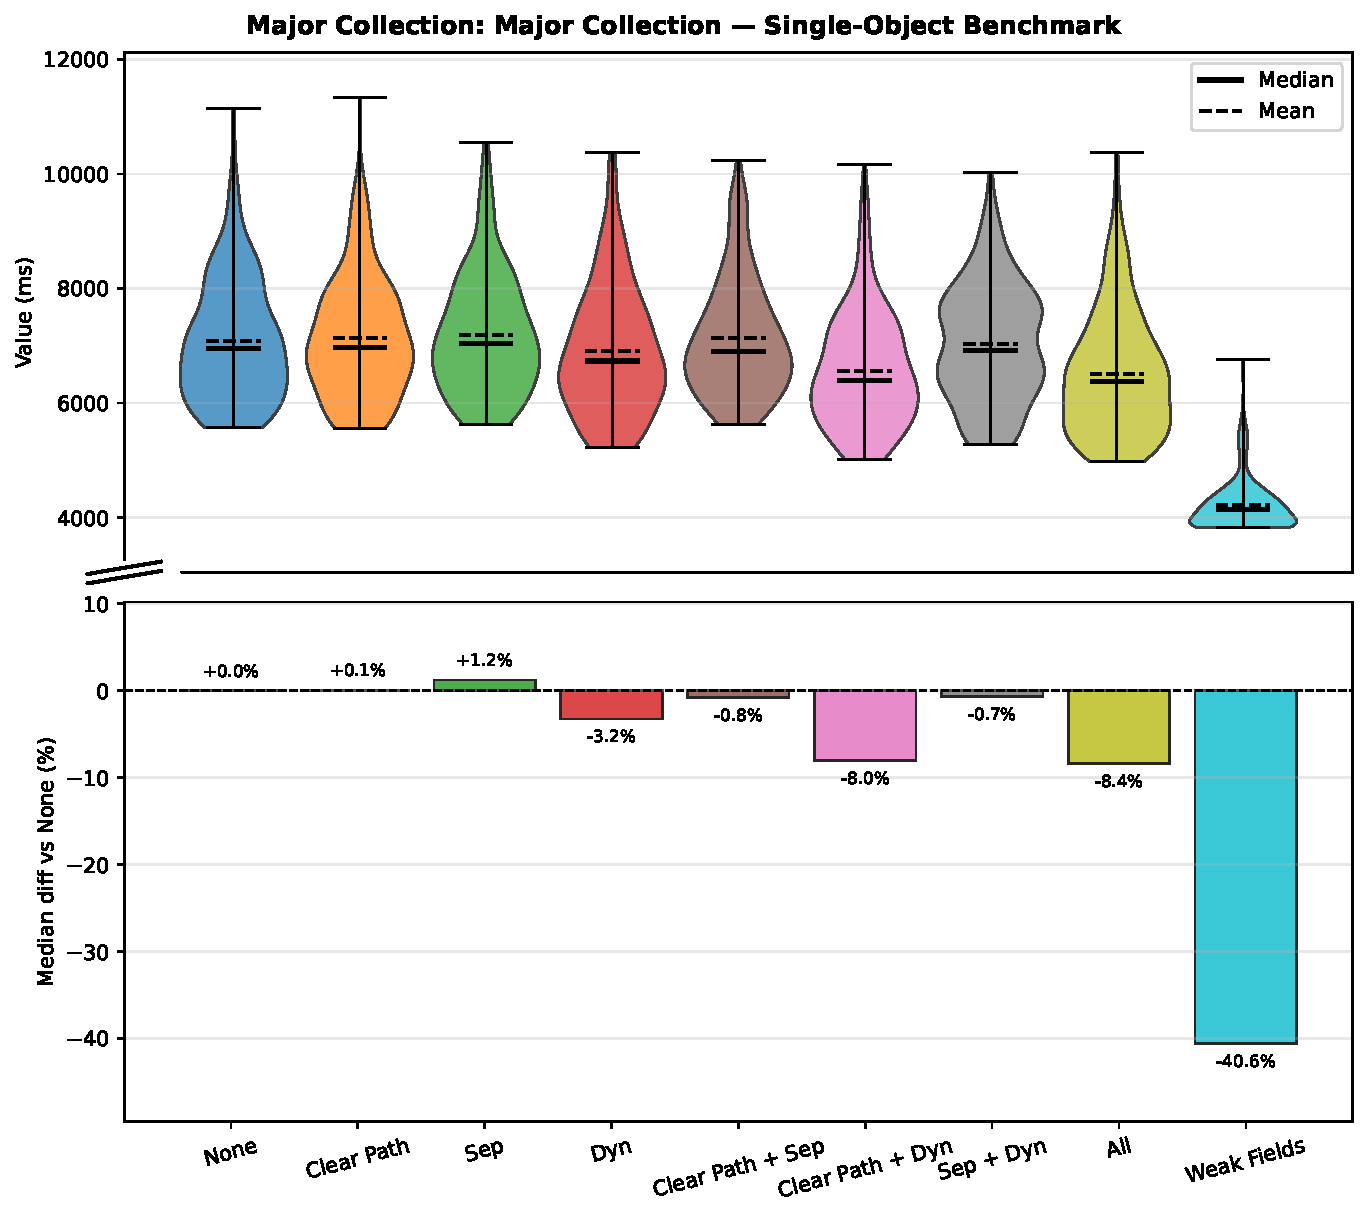
\includegraphics[width=\textwidth]{composite_major_collection_major_collection_slurm-5118807_combined_gc_single.pdf}
%DIFDELCMD < 	%%%
\DIFdelendFL \DIFaddbeginFL 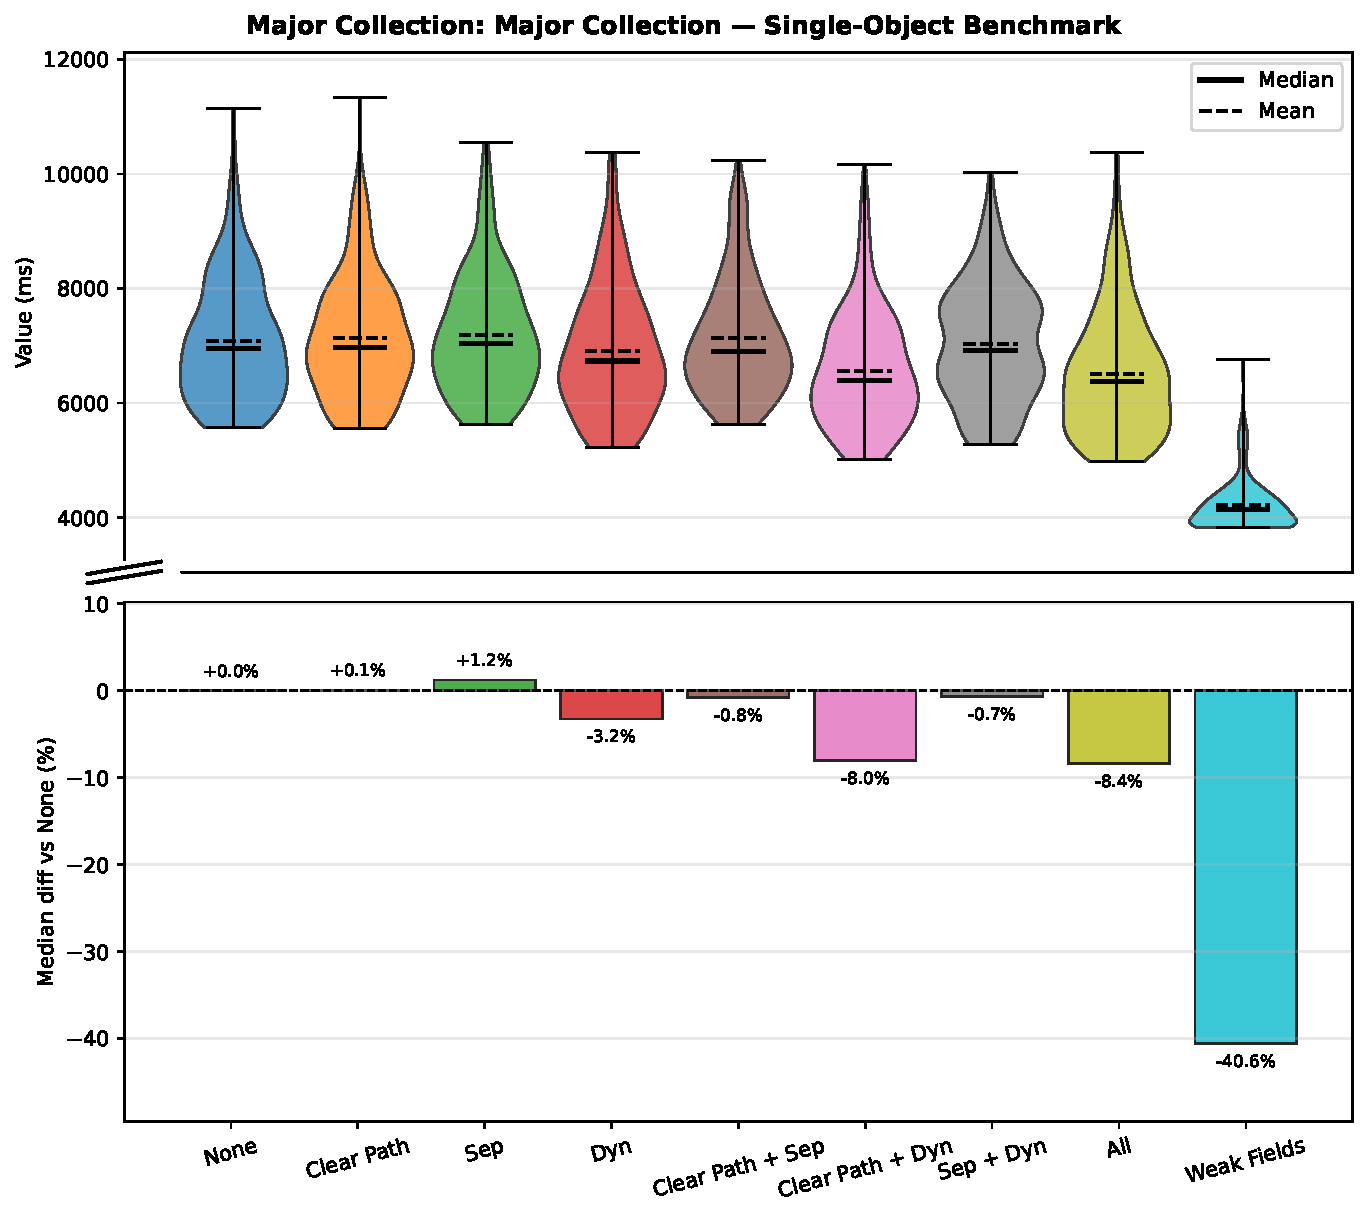
\includegraphics[width=0.8\textwidth]{composite_major_collection_major_collection_slurm-5118807_combined_gc_single.pdf}
	\DIFaddendFL \caption[Major Collection timing (single-object)]{Major Collection timing, \DIFdelbeginFL \DIFdelFL{single-object benchmark }\DIFdelendFL \DIFaddbeginFL \textbf{\DIFaddFL{single-object benchmark}} \DIFaddendFL (per-run maxima). Lower is better. Top: distribution, bottom: median \,\% difference vs baseline.}
	\label{fig:gc-single-major}
\end{figure}

% ---------- Major Collection – multi ----------
\begin{figure}[t]
	\centering
	\DIFdelbeginFL %DIFDELCMD < 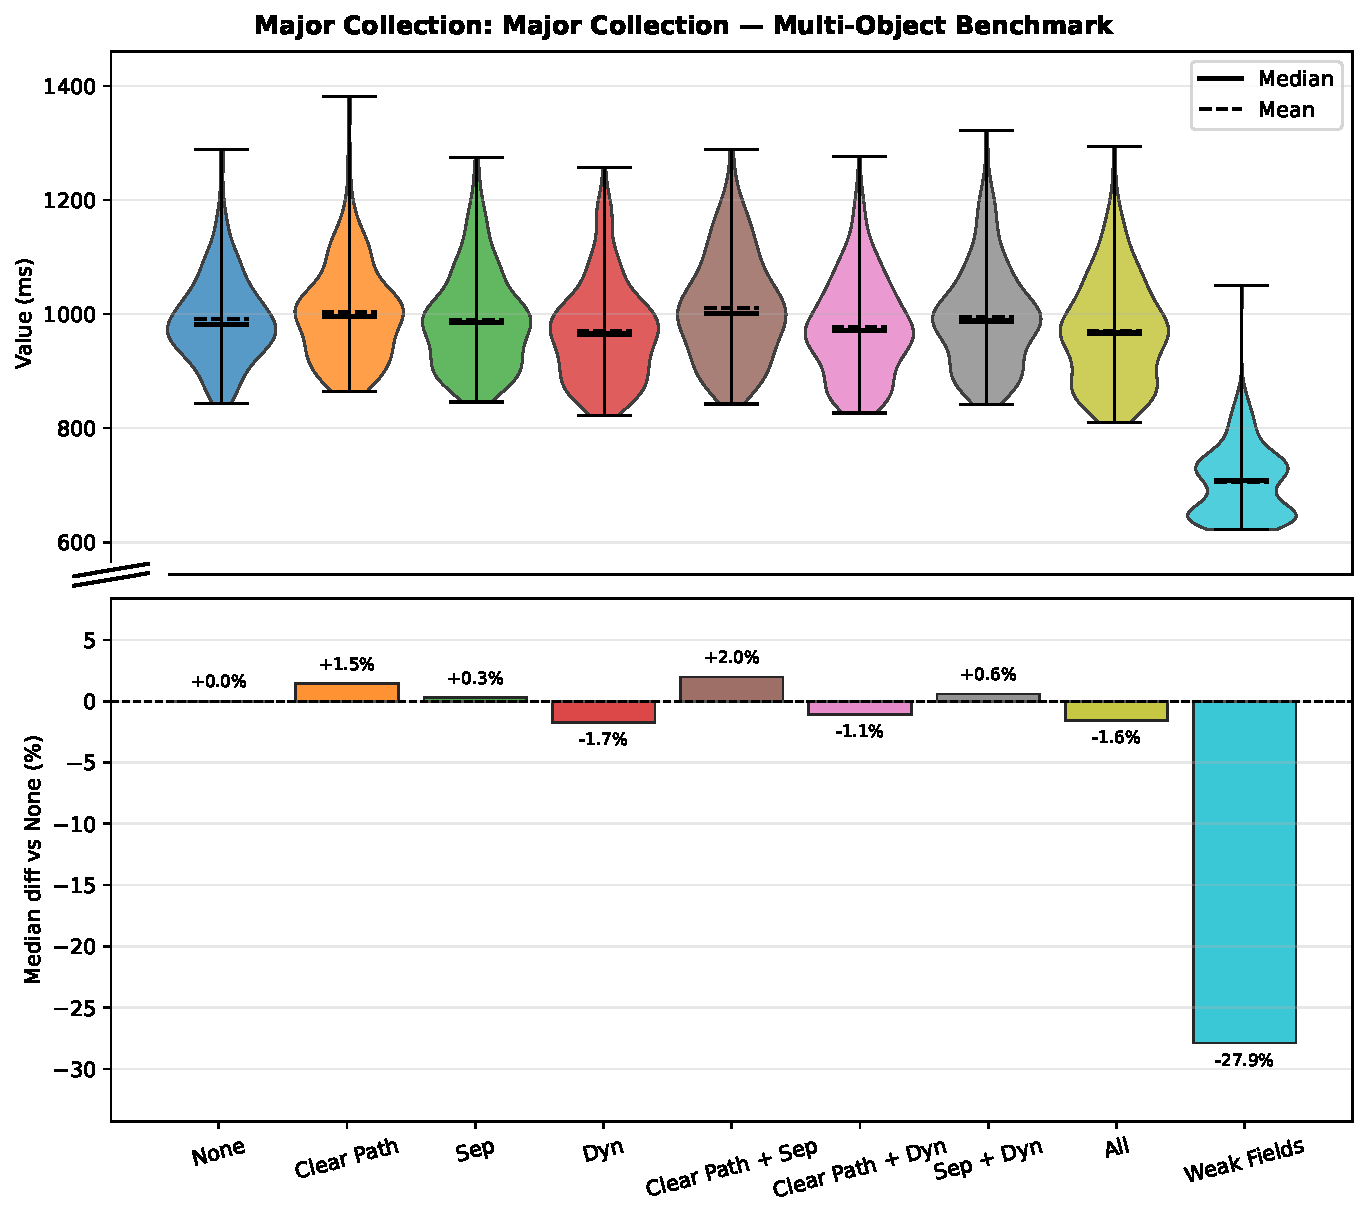
\includegraphics[width=\textwidth]{composite_major_collection_major_collection_slurm-5118807_combined_gc_multi.pdf}
%DIFDELCMD < 	%%%
\DIFdelendFL \DIFaddbeginFL 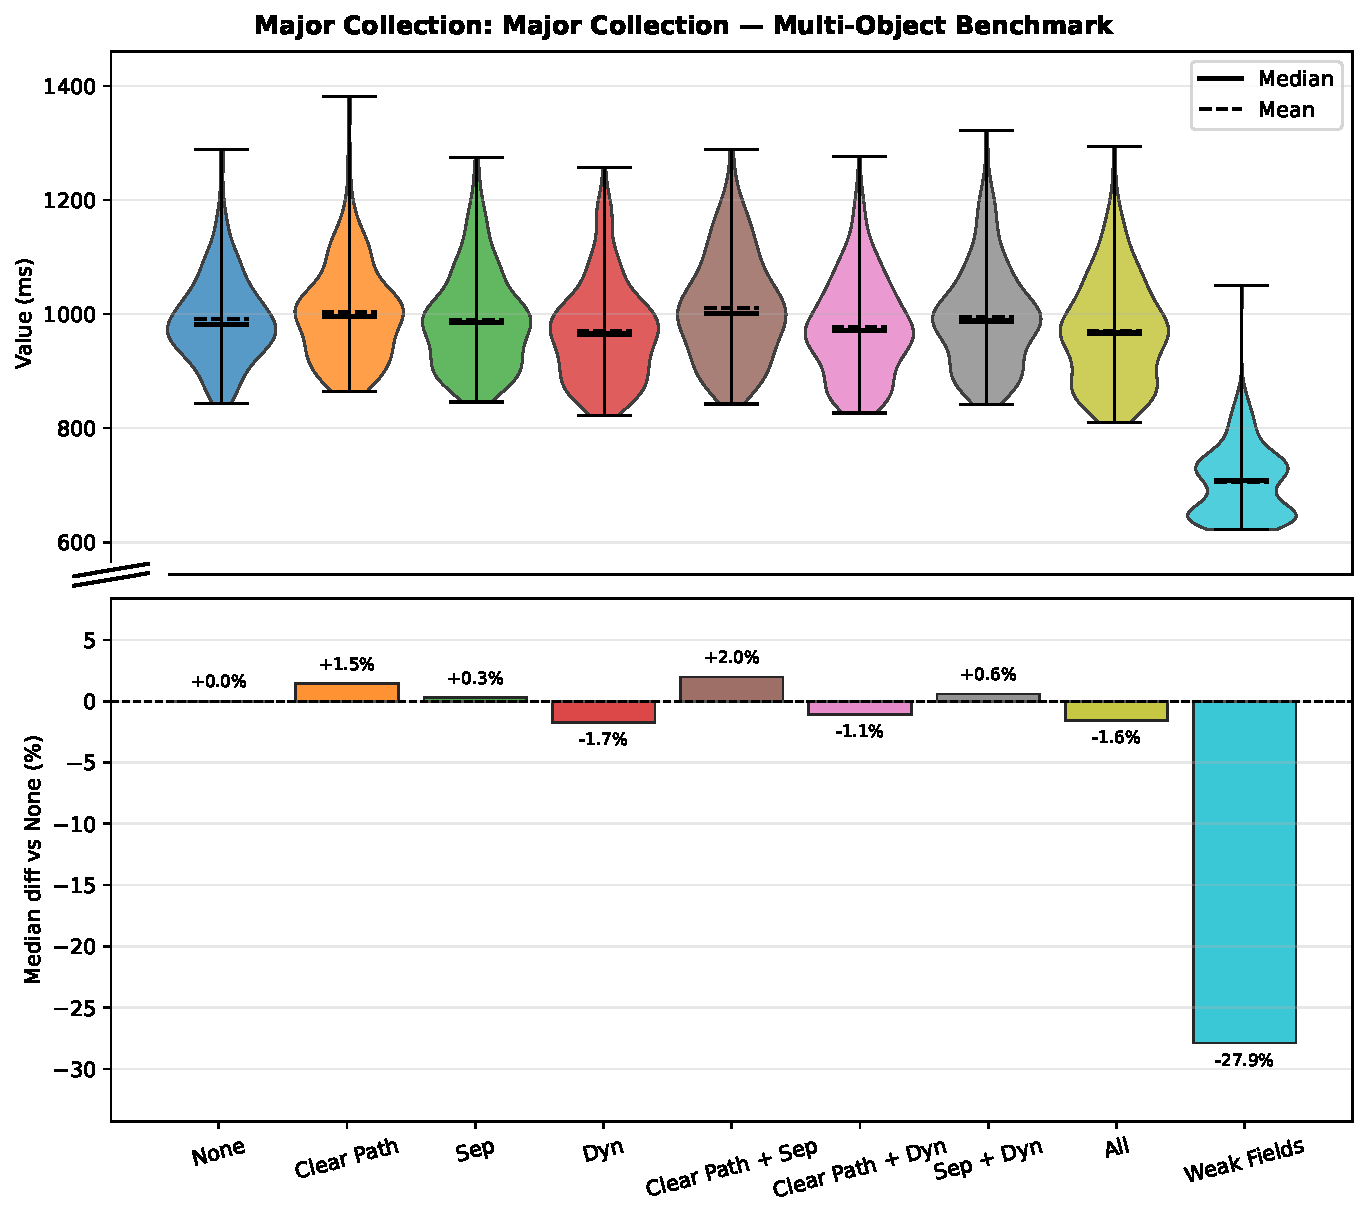
\includegraphics[width=0.8\textwidth]{composite_major_collection_major_collection_slurm-5118807_combined_gc_multi.pdf}
	\DIFaddendFL \caption[Major Collection timing (multi-object)]{Major Collection timing, \DIFdelbeginFL \DIFdelFL{multi-object benchmark }\DIFdelendFL \DIFaddbeginFL \textbf{\DIFaddFL{multi-object benchmark}} \DIFaddendFL (per-run averages). Lower is better. Top: distribution, bottom: median \,\% difference vs baseline.}
	\label{fig:gc-multi-major}
\end{figure}

% ---------- Old Generation – single ----------
\begin{figure}[t]
	\centering
	\DIFdelbeginFL %DIFDELCMD < 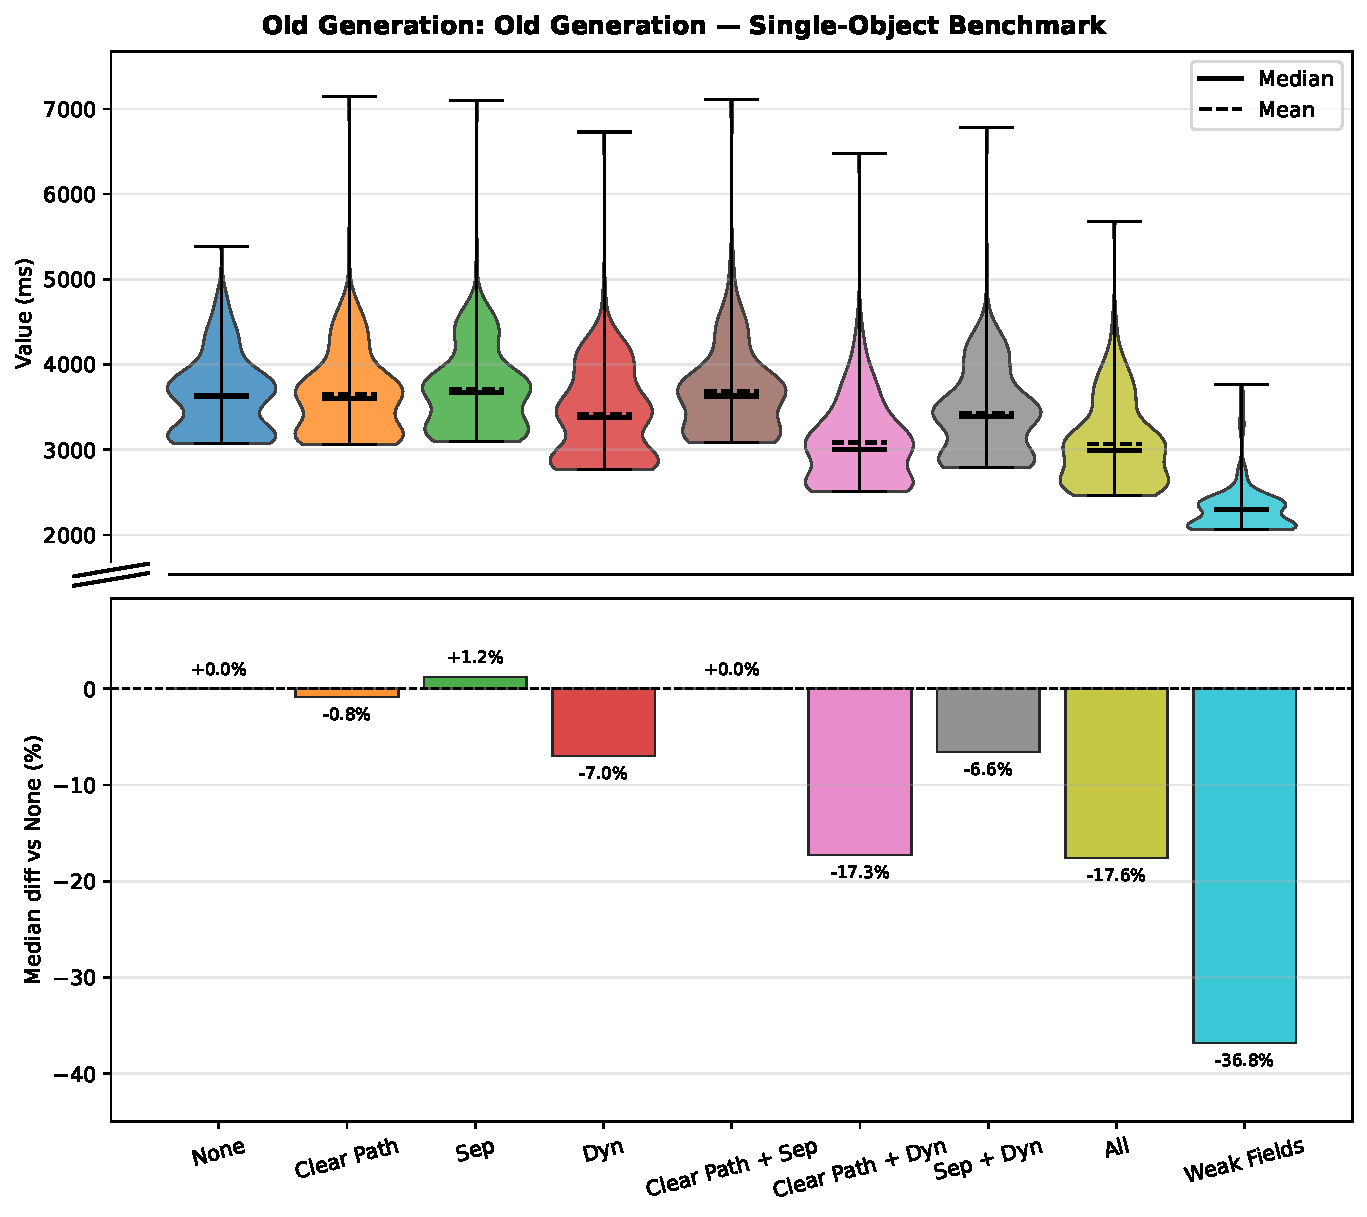
\includegraphics[width=\textwidth]{composite_old_generation_old_generation_slurm-5118807_combined_gc_single.pdf}
%DIFDELCMD < 	%%%
\DIFdelendFL \DIFaddbeginFL 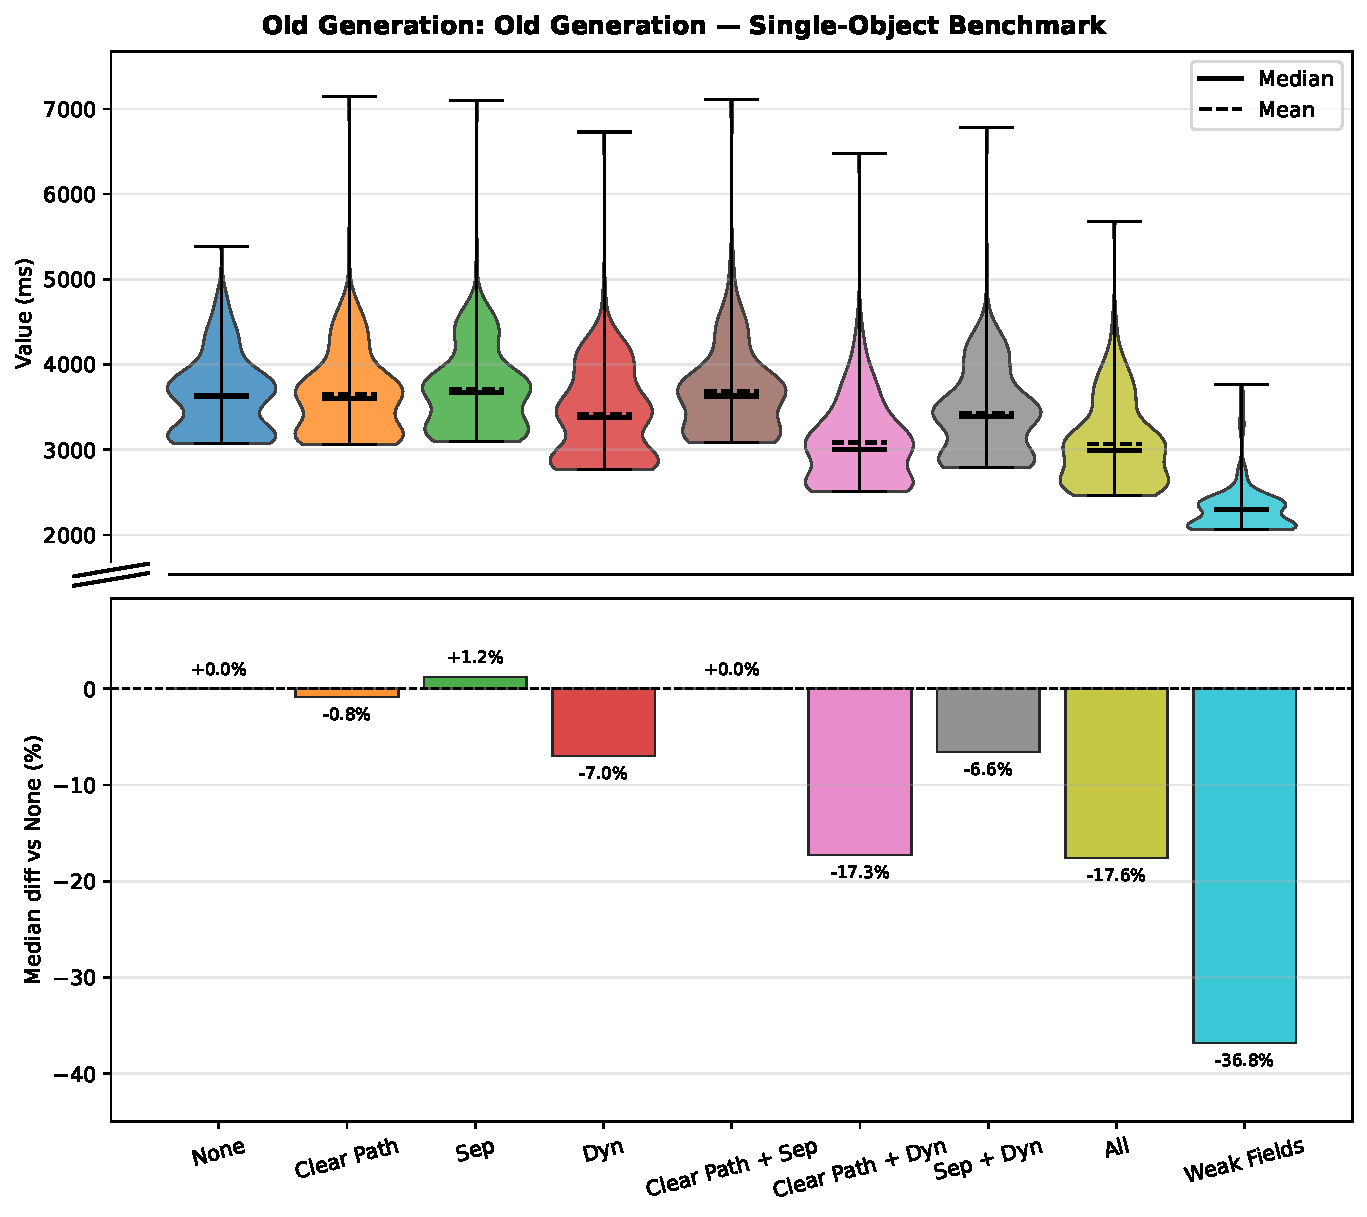
\includegraphics[width=0.8\textwidth]{composite_old_generation_old_generation_slurm-5118807_combined_gc_single.pdf}
	\DIFaddendFL \caption[Old Generation timing (single-object)]{Old Generation timing, \DIFdelbeginFL \DIFdelFL{single-object benchmark }\DIFdelendFL \DIFaddbeginFL \textbf{\DIFaddFL{single-object benchmark}} \DIFaddendFL (per-run maxima). Lower is better. Top: distribution, bottom: median \,\% difference vs baseline.}
	\label{fig:gc-single-old-gen}
\end{figure}

% ---------- Old Generation – multi ----------
\begin{figure}[t]
	\centering
	\DIFdelbeginFL %DIFDELCMD < 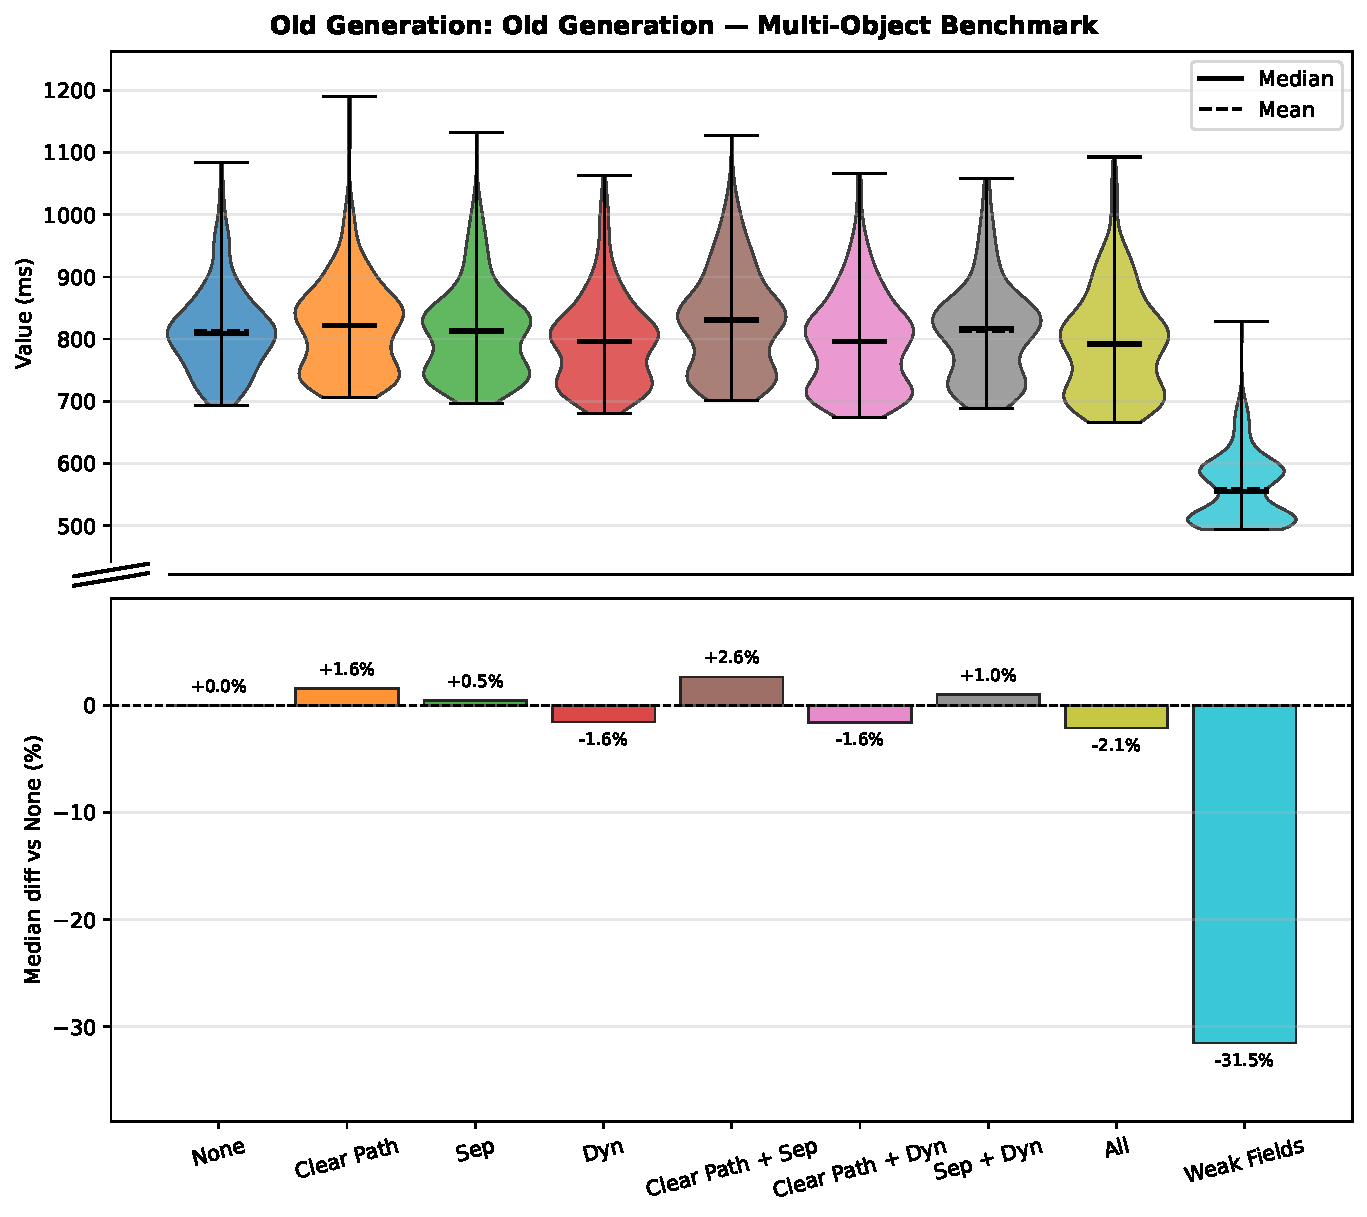
\includegraphics[width=\textwidth]{composite_old_generation_old_generation_slurm-5118807_combined_gc_multi.pdf}
%DIFDELCMD < 	%%%
\DIFdelendFL \DIFaddbeginFL 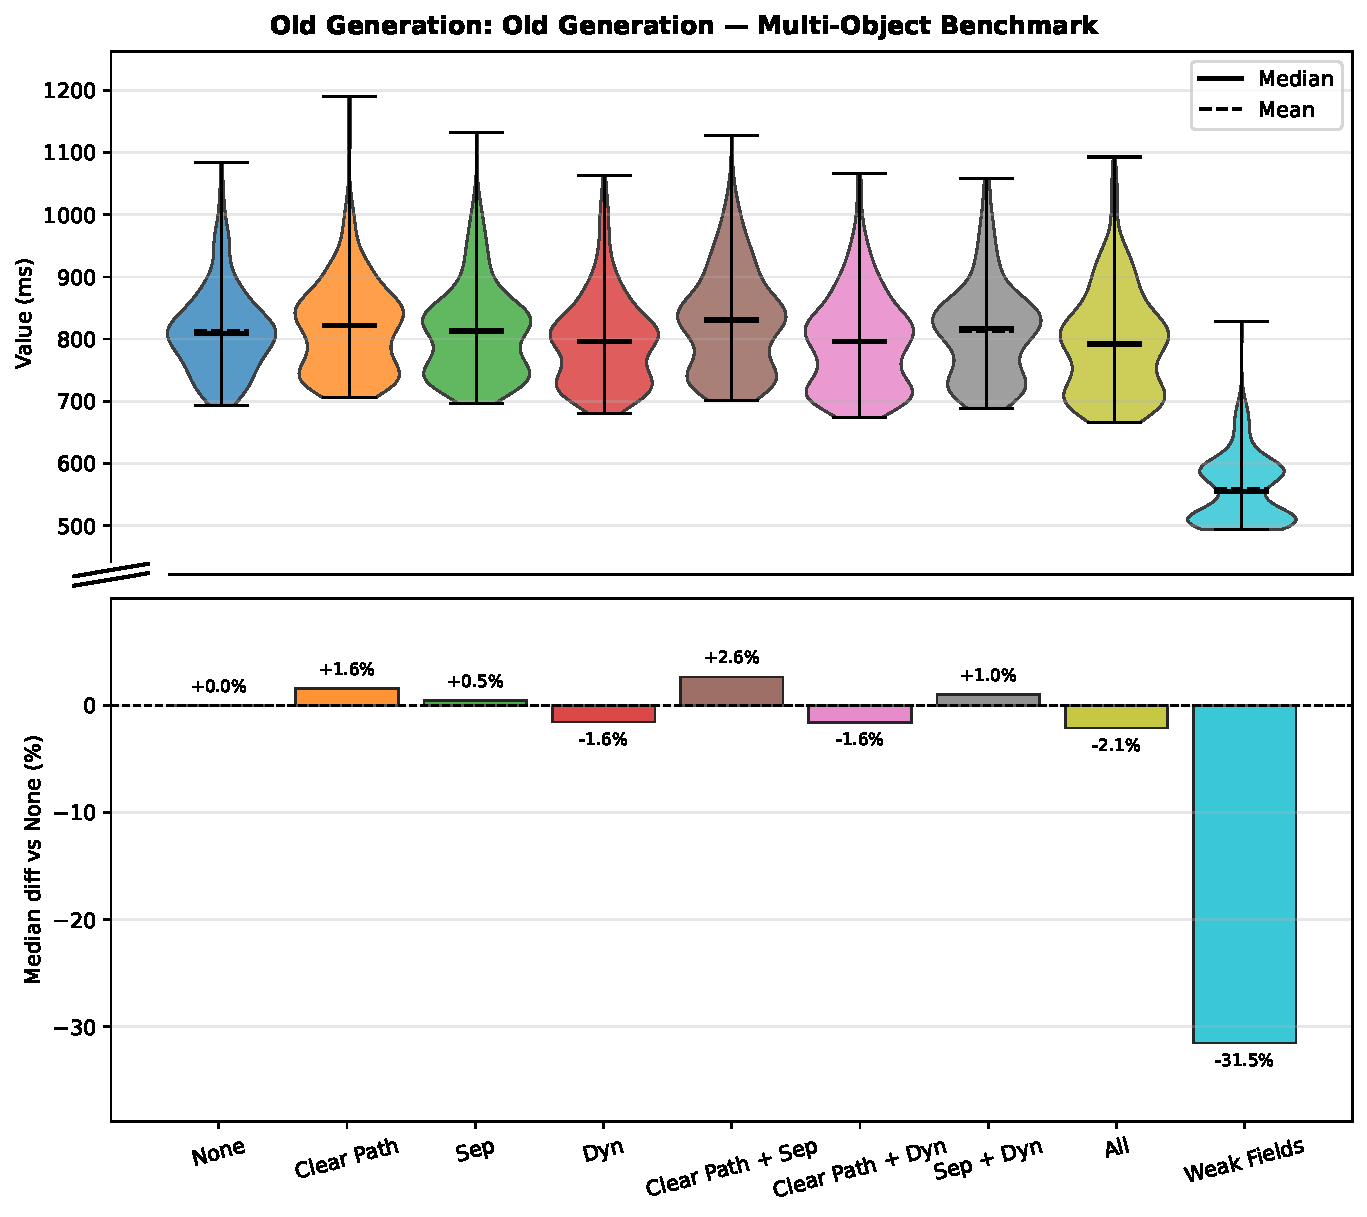
\includegraphics[width=0.8\textwidth]{composite_old_generation_old_generation_slurm-5118807_combined_gc_multi.pdf}
	\DIFaddendFL \caption[Old Generation timing (multi-object)]{Old Generation timing, \DIFdelbeginFL \DIFdelFL{multi-object benchmark }\DIFdelendFL \DIFaddbeginFL \textbf{\DIFaddFL{multi-object benchmark}} \DIFaddendFL (per-run averages). Lower is better. Top: distribution, bottom: median \,\% difference vs baseline.}
	\label{fig:gc-multi-old-gen}
\end{figure}

% ---------- Old Phase: Concurrent Mark – single ----------
\begin{figure}[t]
	\centering
	\DIFdelbeginFL %DIFDELCMD < 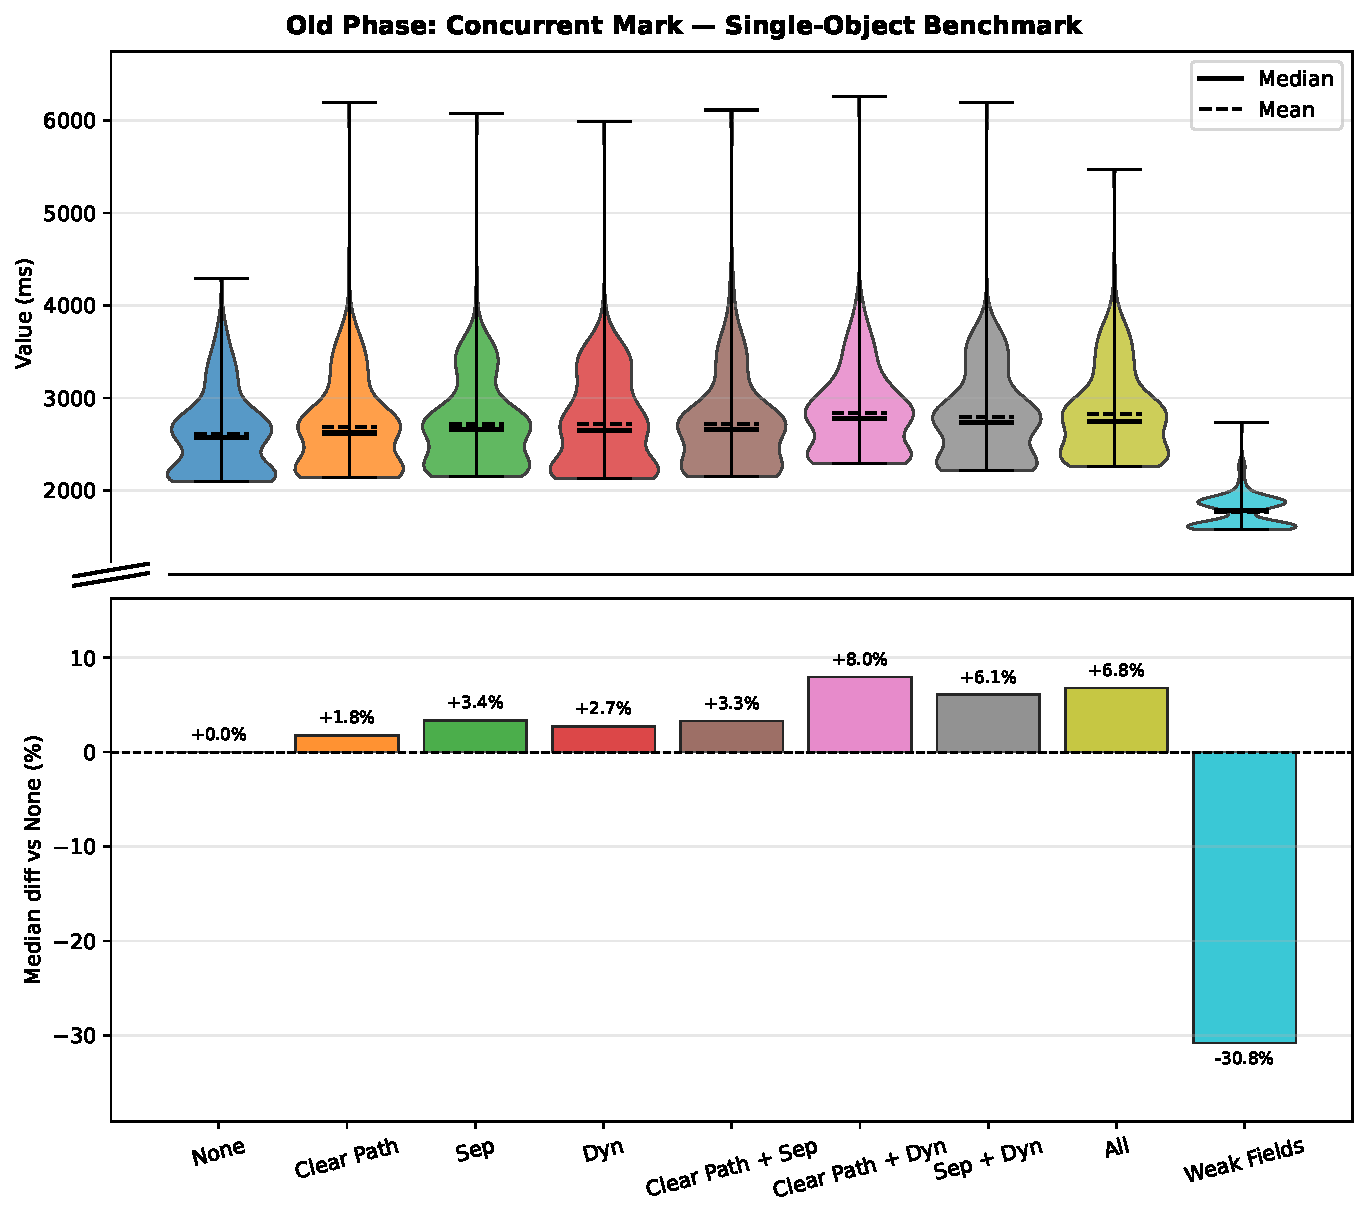
\includegraphics[width=\textwidth]{composite_old_phase_concurrent_mark_slurm-5118807_combined_gc_single.pdf}
%DIFDELCMD < 	%%%
\DIFdelendFL \DIFaddbeginFL 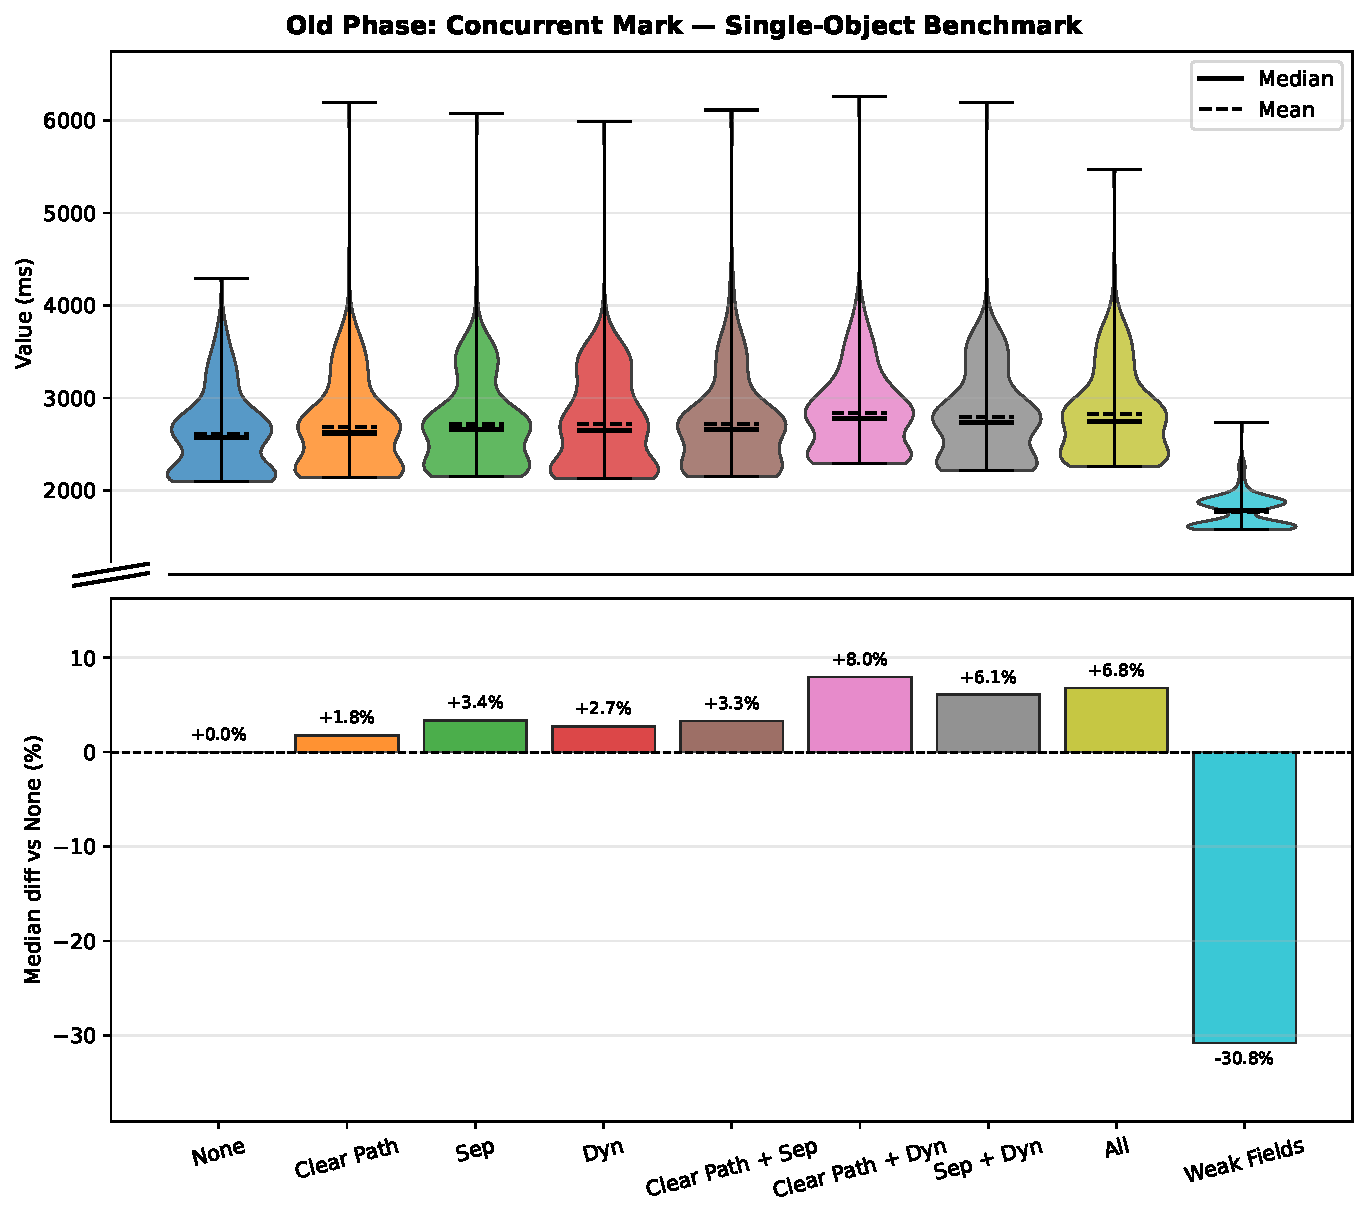
\includegraphics[width=0.8\textwidth]{composite_old_phase_concurrent_mark_slurm-5118807_combined_gc_single.pdf}
	\DIFaddendFL \caption[Old Phase: Concurrent Mark timing (single-object)]{Old Phase: Concurrent Mark timing, \DIFdelbeginFL \DIFdelFL{single-object benchmark }\DIFdelendFL \DIFaddbeginFL \textbf{\DIFaddFL{single-object benchmark}} \DIFaddendFL (per-run maxima). Lower is better. Top: distribution, bottom: median \,\% difference vs baseline.}
	\label{fig:gc-single-old-mark}
\end{figure}

% ---------- Old Phase: Concurrent Mark – multi ----------
\begin{figure}[t]
	\centering
	\DIFdelbeginFL %DIFDELCMD < 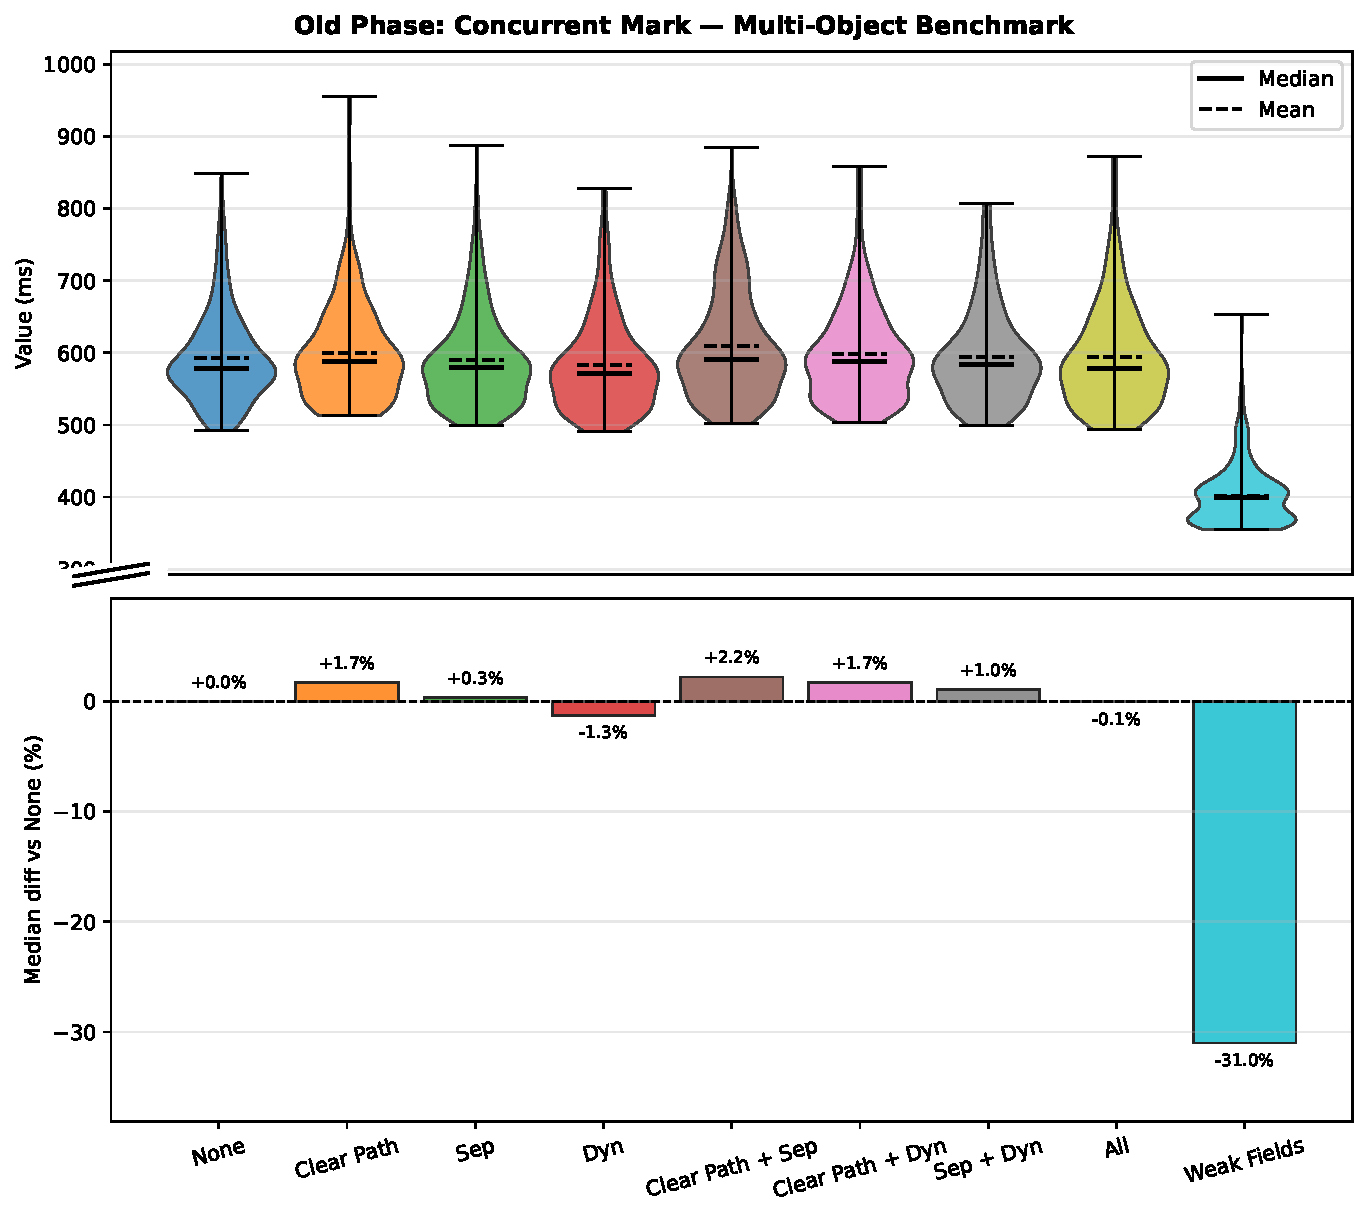
\includegraphics[width=\textwidth]{composite_old_phase_concurrent_mark_slurm-5118807_combined_gc_multi.pdf}
%DIFDELCMD < 	%%%
\DIFdelendFL \DIFaddbeginFL 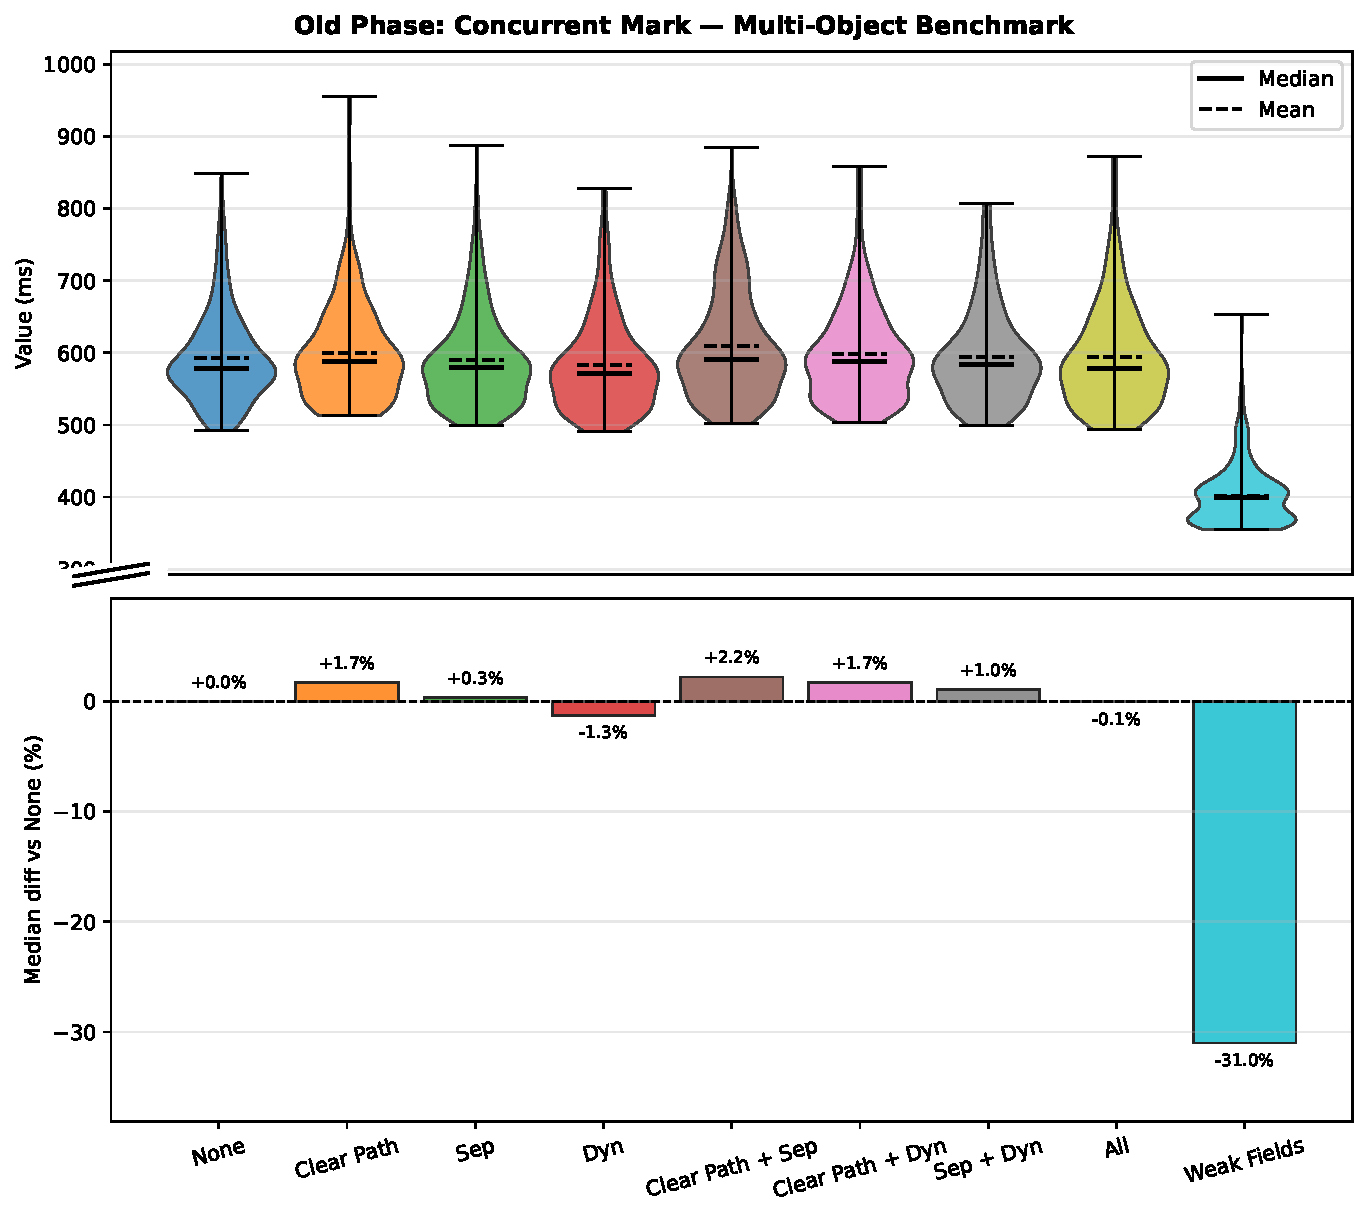
\includegraphics[width=0.8\textwidth]{composite_old_phase_concurrent_mark_slurm-5118807_combined_gc_multi.pdf}
	\DIFaddendFL \caption[Old Phase: Concurrent Mark timing (multi-object)]{Old Phase: Concurrent Mark timing, \DIFdelbeginFL \DIFdelFL{multi-object benchmark }\DIFdelendFL \DIFaddbeginFL \textbf{\DIFaddFL{multi-object benchmark}} \DIFaddendFL (per-run averages). Lower is better. Top: distribution, bottom: median \,\% difference vs baseline.}
	\label{fig:gc-multi-old-mark}
\end{figure}

% ---------- Old Phase: Concurrent Process Non-Strong – single ----------
\begin{figure}[t]
	\centering
	\DIFdelbeginFL %DIFDELCMD < 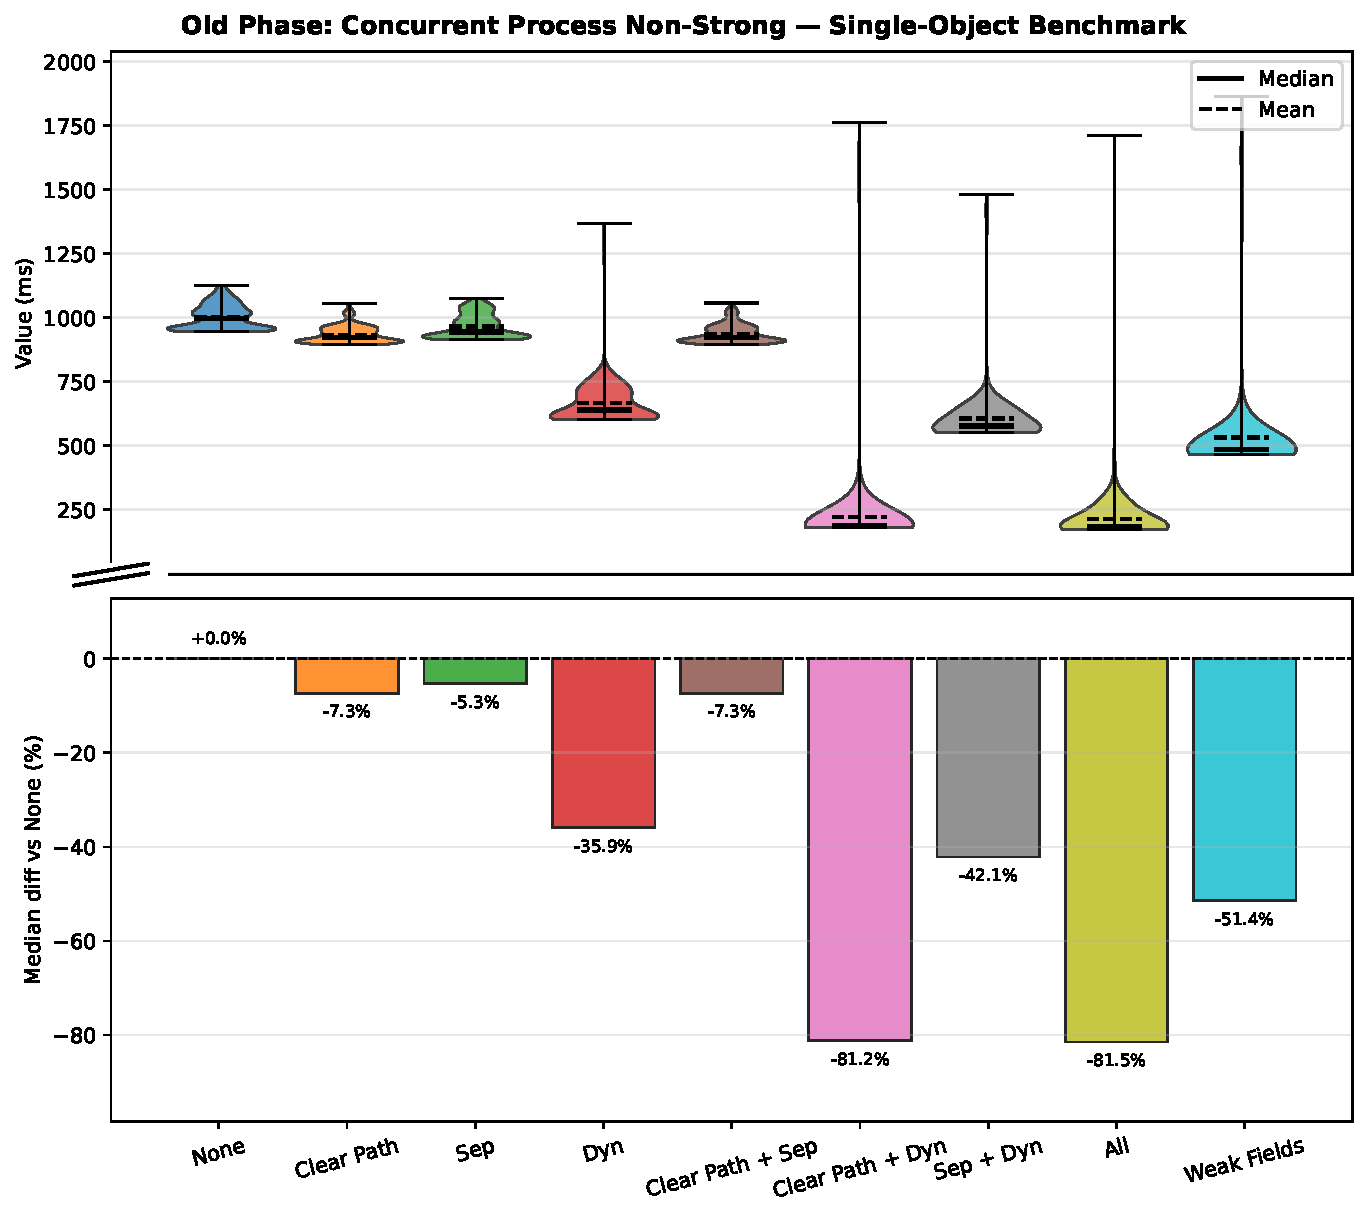
\includegraphics[width=\textwidth]{composite_old_phase_concurrent_process_non-strong_slurm-5118807_combined_gc_single.pdf}
%DIFDELCMD < 	%%%
\DIFdelendFL \DIFaddbeginFL 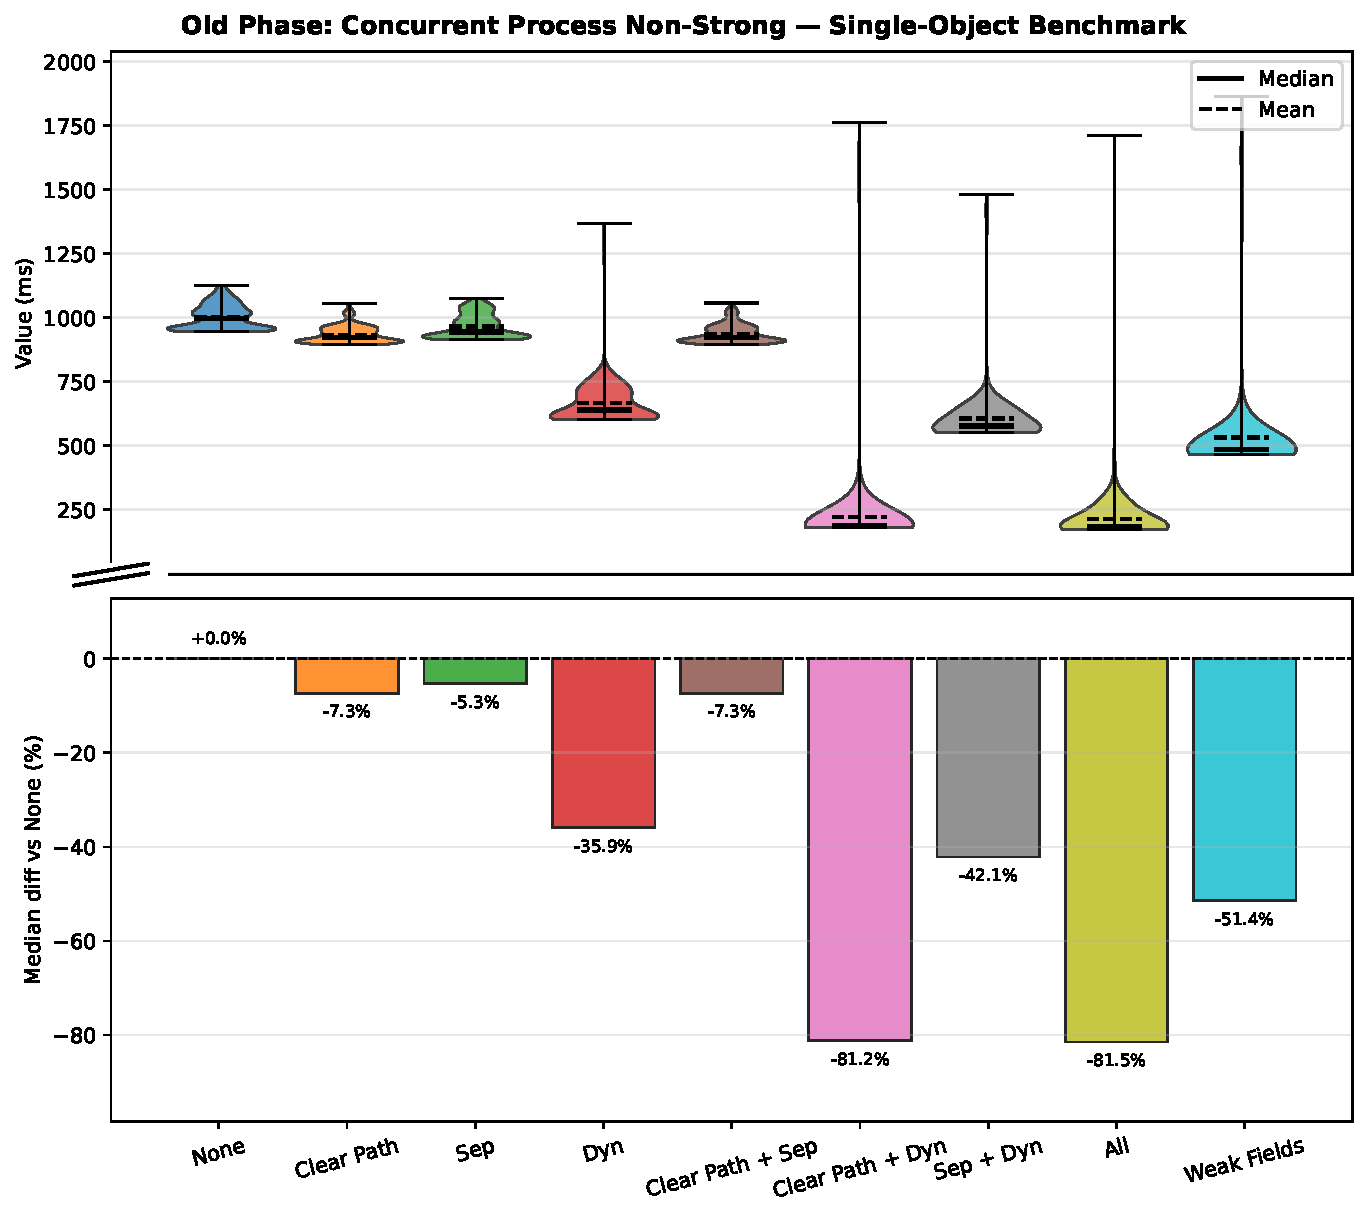
\includegraphics[width=0.8\textwidth]{composite_old_phase_concurrent_process_non-strong_slurm-5118807_combined_gc_single.pdf}
	\DIFaddendFL \caption[Old Phase: Concurrent Process Non-Strong timing (single-object)]{Old Phase: Concurrent Process Non-Strong timing, \DIFdelbeginFL \DIFdelFL{single-object benchmark }\DIFdelendFL \DIFaddbeginFL \textbf{\DIFaddFL{single-object benchmark}} \DIFaddendFL (per-run maxima). Lower is better. Top: distribution, bottom: median \,\% difference vs baseline.}
	\label{fig:gc-single-nonstrong}
\end{figure}

% ---------- Old Phase: Concurrent Process Non-Strong – multi ----------
\begin{figure}[t]
	\centering
	\DIFdelbeginFL %DIFDELCMD < 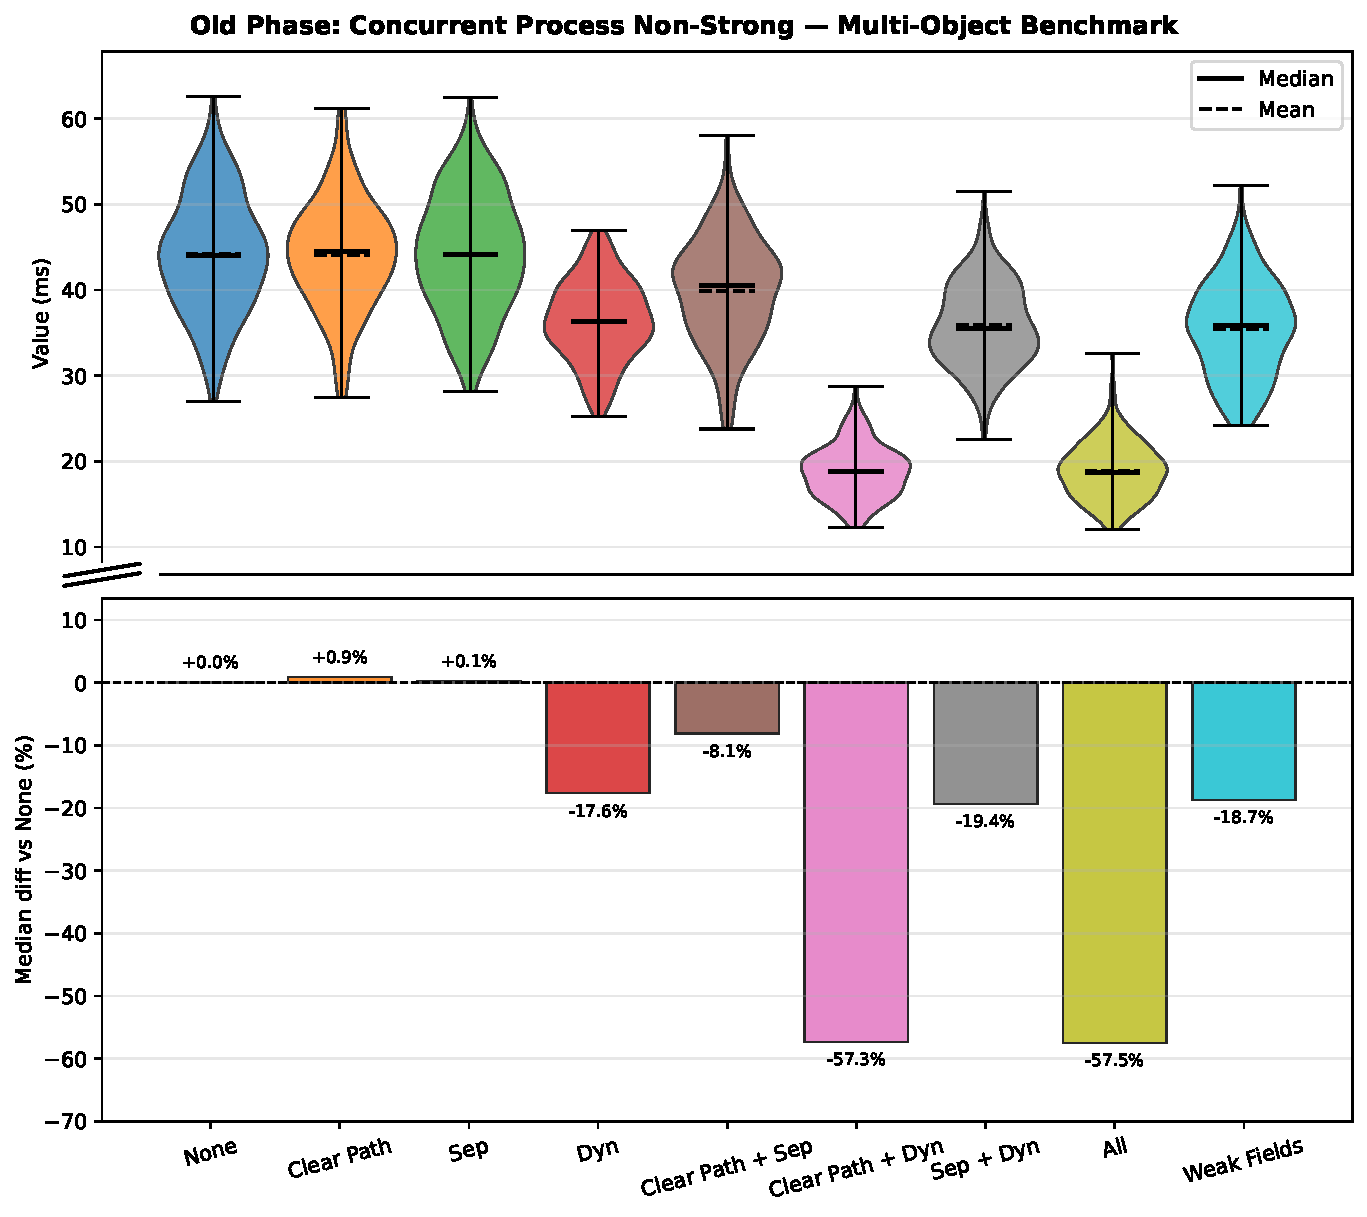
\includegraphics[width=\textwidth]{composite_old_phase_concurrent_process_non-strong_slurm-5118807_combined_gc_multi.pdf}
%DIFDELCMD < 	%%%
\DIFdelendFL \DIFaddbeginFL 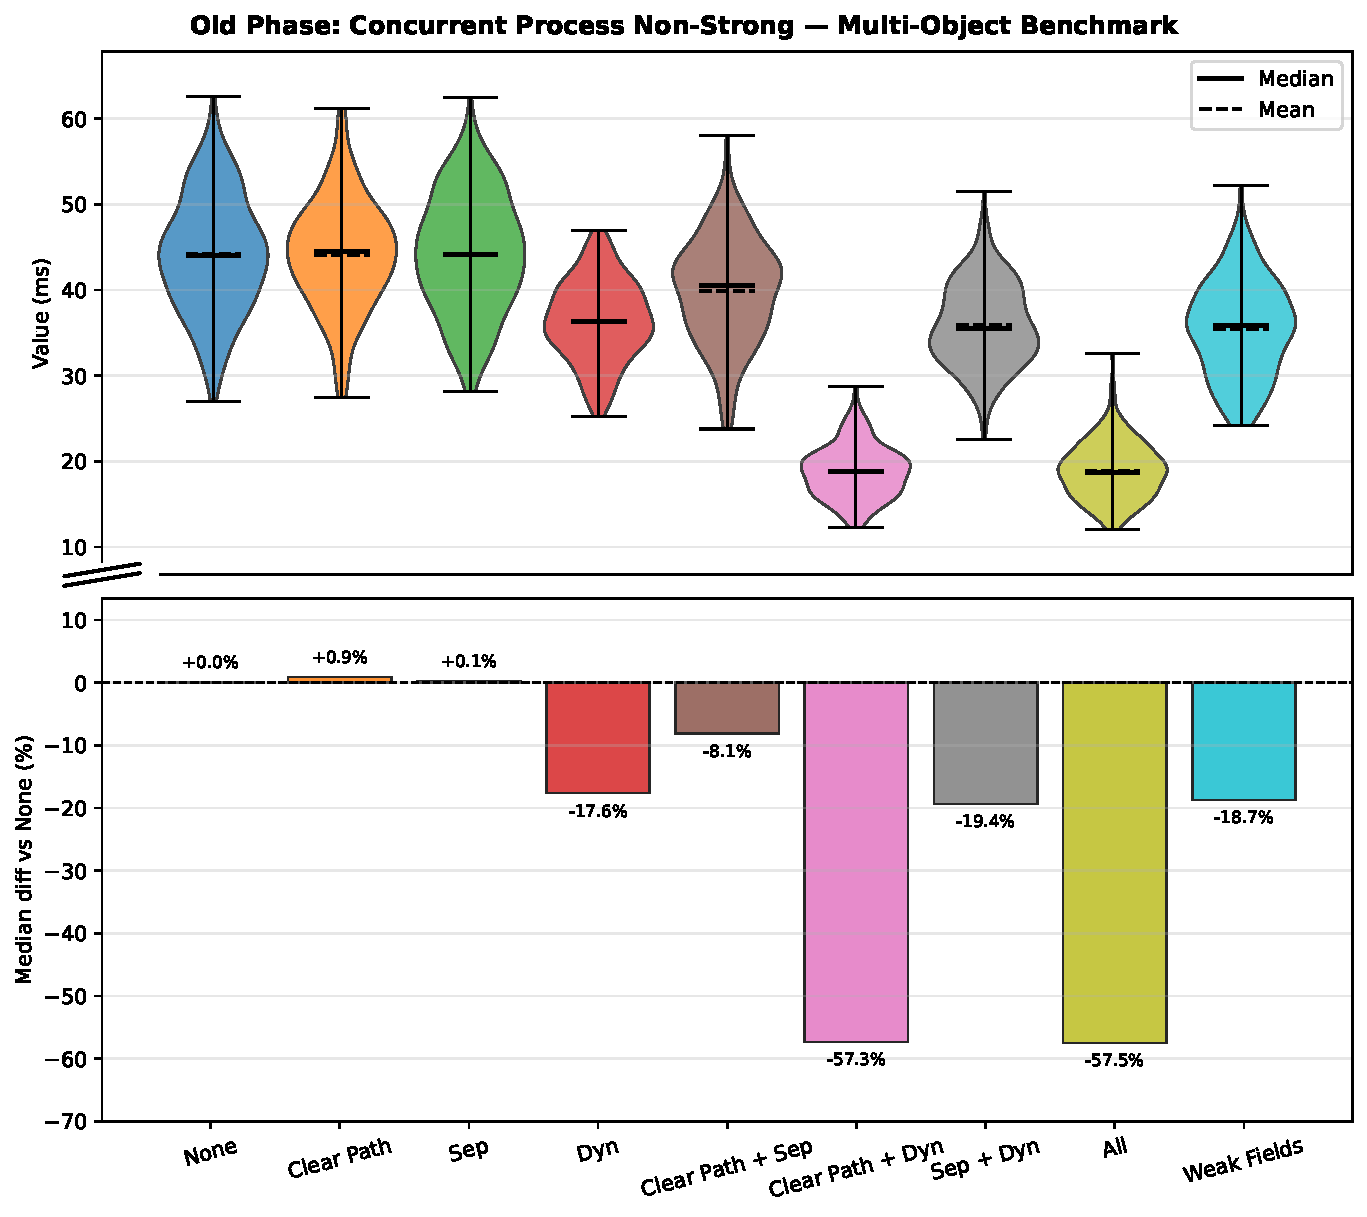
\includegraphics[width=0.8\textwidth]{composite_old_phase_concurrent_process_non-strong_slurm-5118807_combined_gc_multi.pdf}
	\DIFaddendFL \caption[Old Phase: Concurrent Process Non-Strong timing (multi-object)]{Old Phase: Concurrent Process Non-Strong timing, \DIFdelbeginFL \DIFdelFL{multi-object benchmark }\DIFdelendFL \DIFaddbeginFL \textbf{\DIFaddFL{multi-object benchmark}} \DIFaddendFL (per-run averages). Lower is better. Top: distribution, bottom: median \,\% difference vs baseline.}
	\label{fig:gc-multi-nonstrong}
\end{figure}

% ---------- Young Generation (Promote All) – single ----------
\begin{figure}[t]
	\centering
	\DIFdelbeginFL %DIFDELCMD < 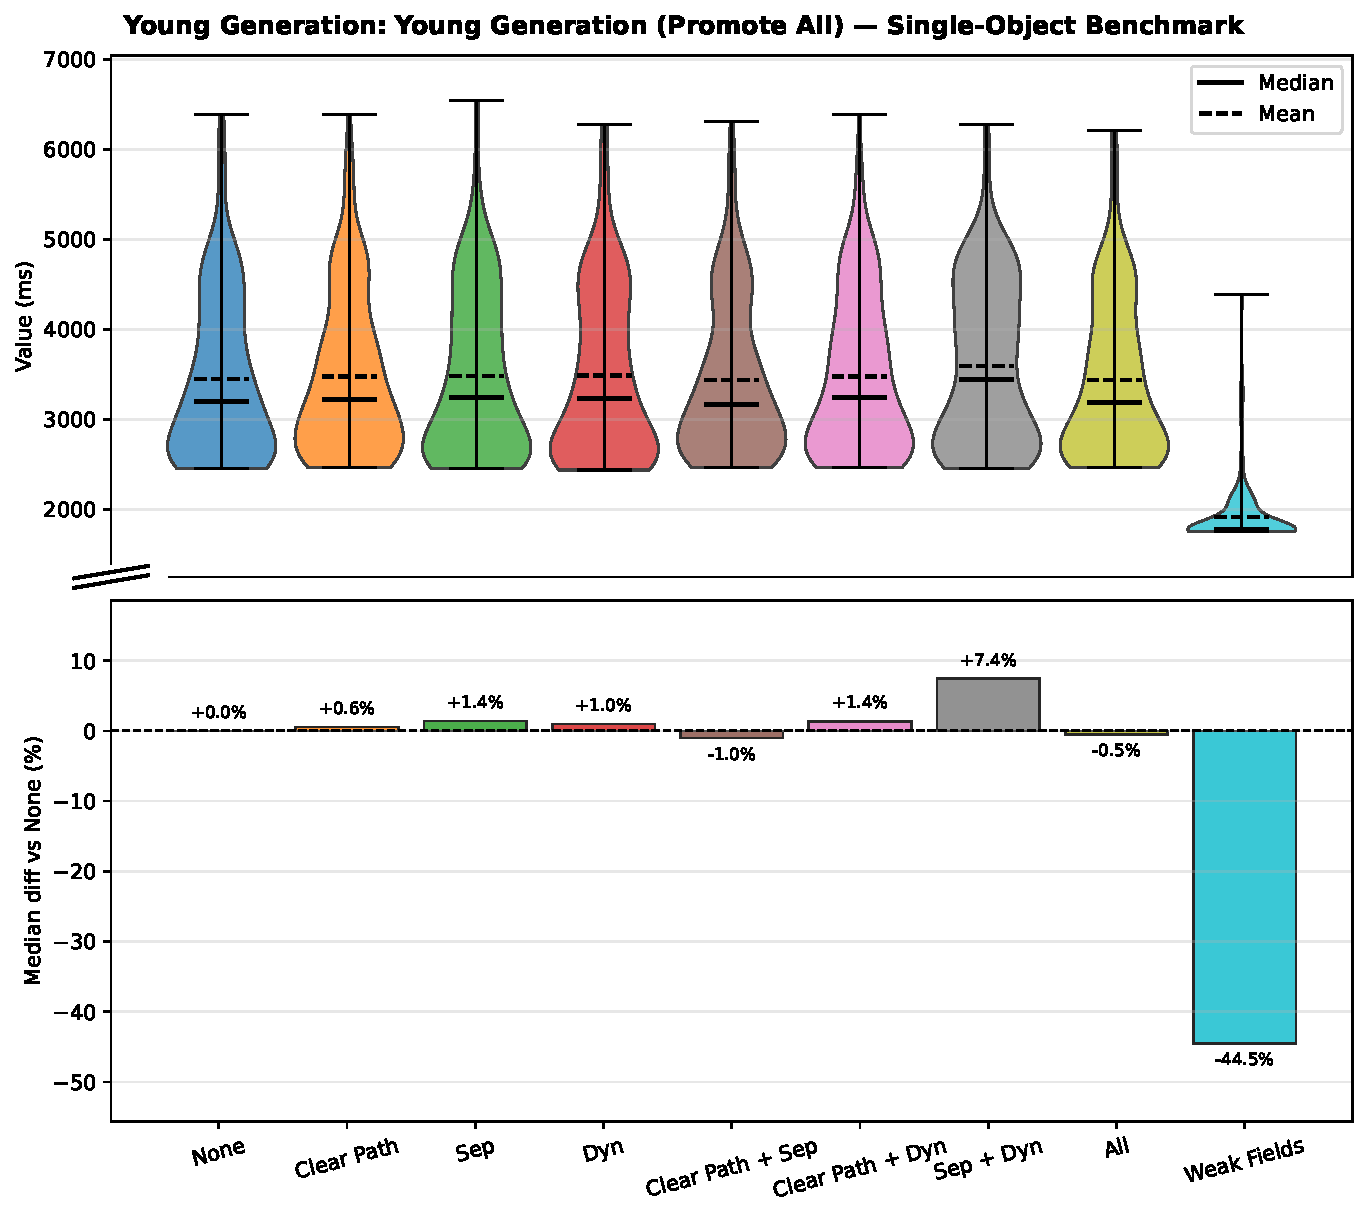
\includegraphics[width=\textwidth]{composite_young_generation_young_generation_promote_all_slurm-5118807_combined_gc_single.pdf}
%DIFDELCMD < 	%%%
\DIFdelendFL \DIFaddbeginFL 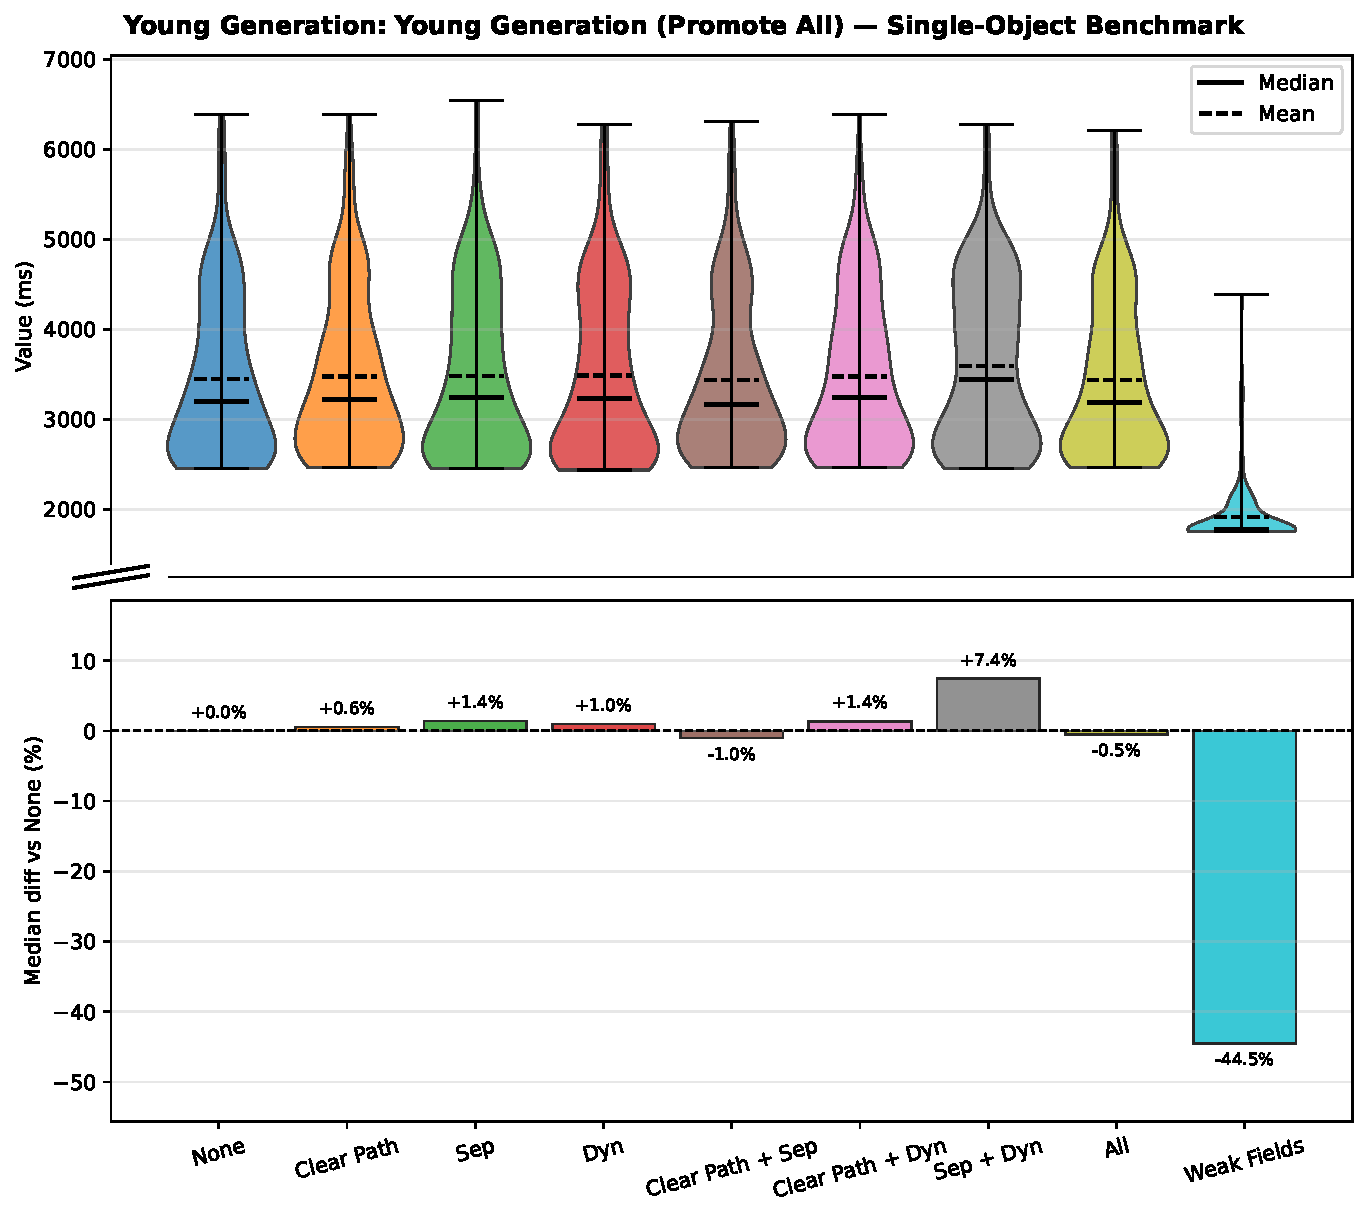
\includegraphics[width=0.8\textwidth]{composite_young_generation_young_generation_promote_all_slurm-5118807_combined_gc_single.pdf}
	\DIFaddendFL \caption[Young Generation (Promote All) timing (single-object)]{Young Generation (Promote All) timing, \DIFdelbeginFL \DIFdelFL{single-object benchmark }\DIFdelendFL \DIFaddbeginFL \textbf{\DIFaddFL{single-object benchmark}} \DIFaddendFL (per-run maxima). Lower is better. Top: distribution, bottom: median \,\% difference vs baseline.}
	\label{fig:gc-single-young-gen}
\end{figure}

% ---------- Young Generation (Promote All) – multi ----------
\begin{figure}[t]
	\centering
	\DIFdelbeginFL %DIFDELCMD < 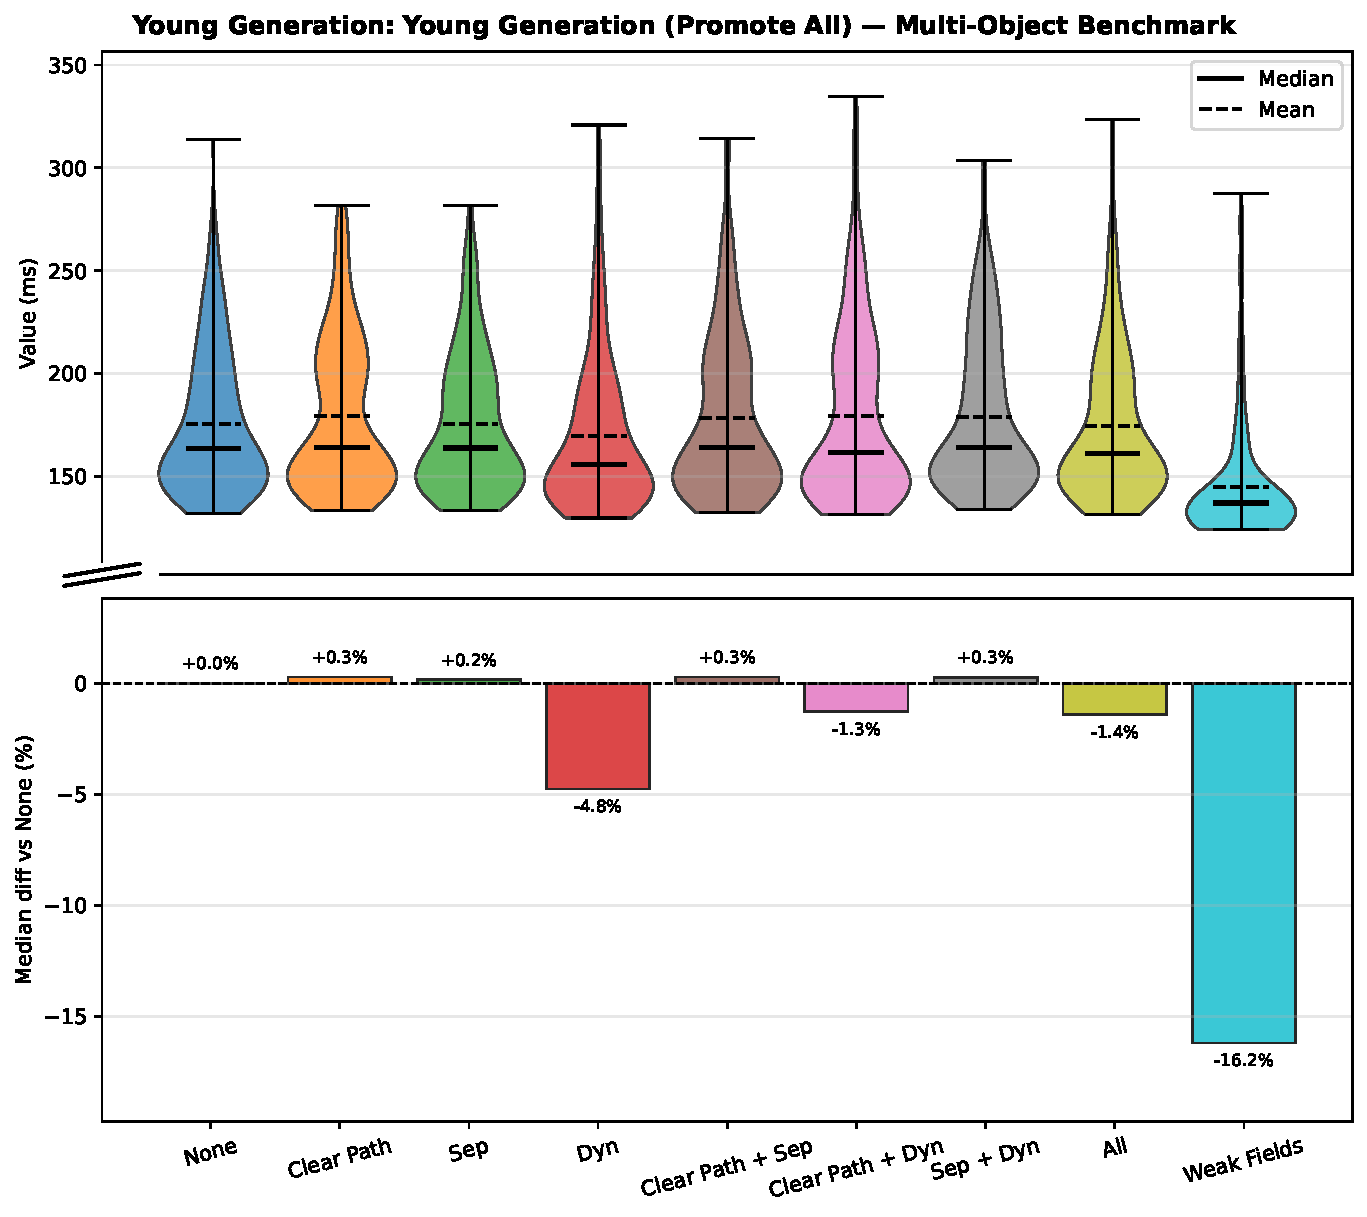
\includegraphics[width=\textwidth]{composite_young_generation_young_generation_promote_all_slurm-5118807_combined_gc_multi.pdf}
%DIFDELCMD < 	%%%
\DIFdelendFL \DIFaddbeginFL 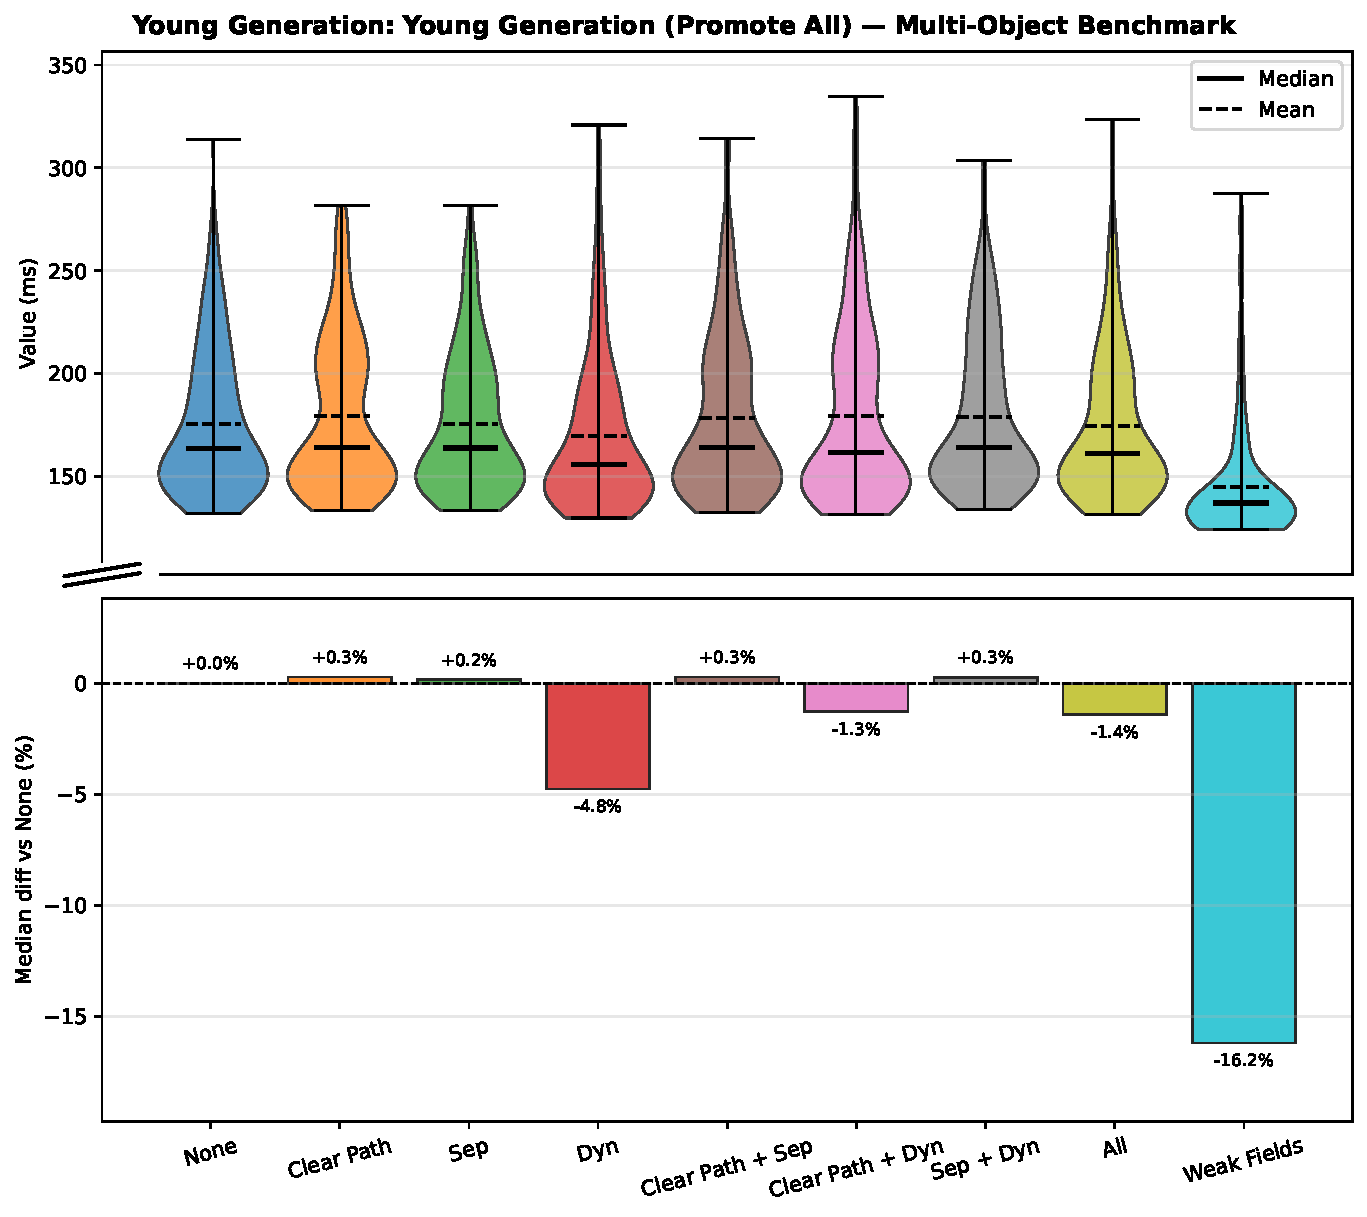
\includegraphics[width=0.8\textwidth]{composite_young_generation_young_generation_promote_all_slurm-5118807_combined_gc_multi.pdf}
	\DIFaddendFL \caption[Young Generation (Promote All) timing (multi-object)]{Young Generation (Promote All) timing, \DIFdelbeginFL \DIFdelFL{multi-object benchmark }\DIFdelendFL \DIFaddbeginFL \textbf{\DIFaddFL{multi-object benchmark}} \DIFaddendFL (per-run averages). Lower is better. Top: distribution, bottom: median \,\% difference vs baseline.}
	\label{fig:gc-multi-young-gen}
\end{figure}

% ---------- Memory median diff histograms – single ----------
\begin{figure}[t]
	\centering
	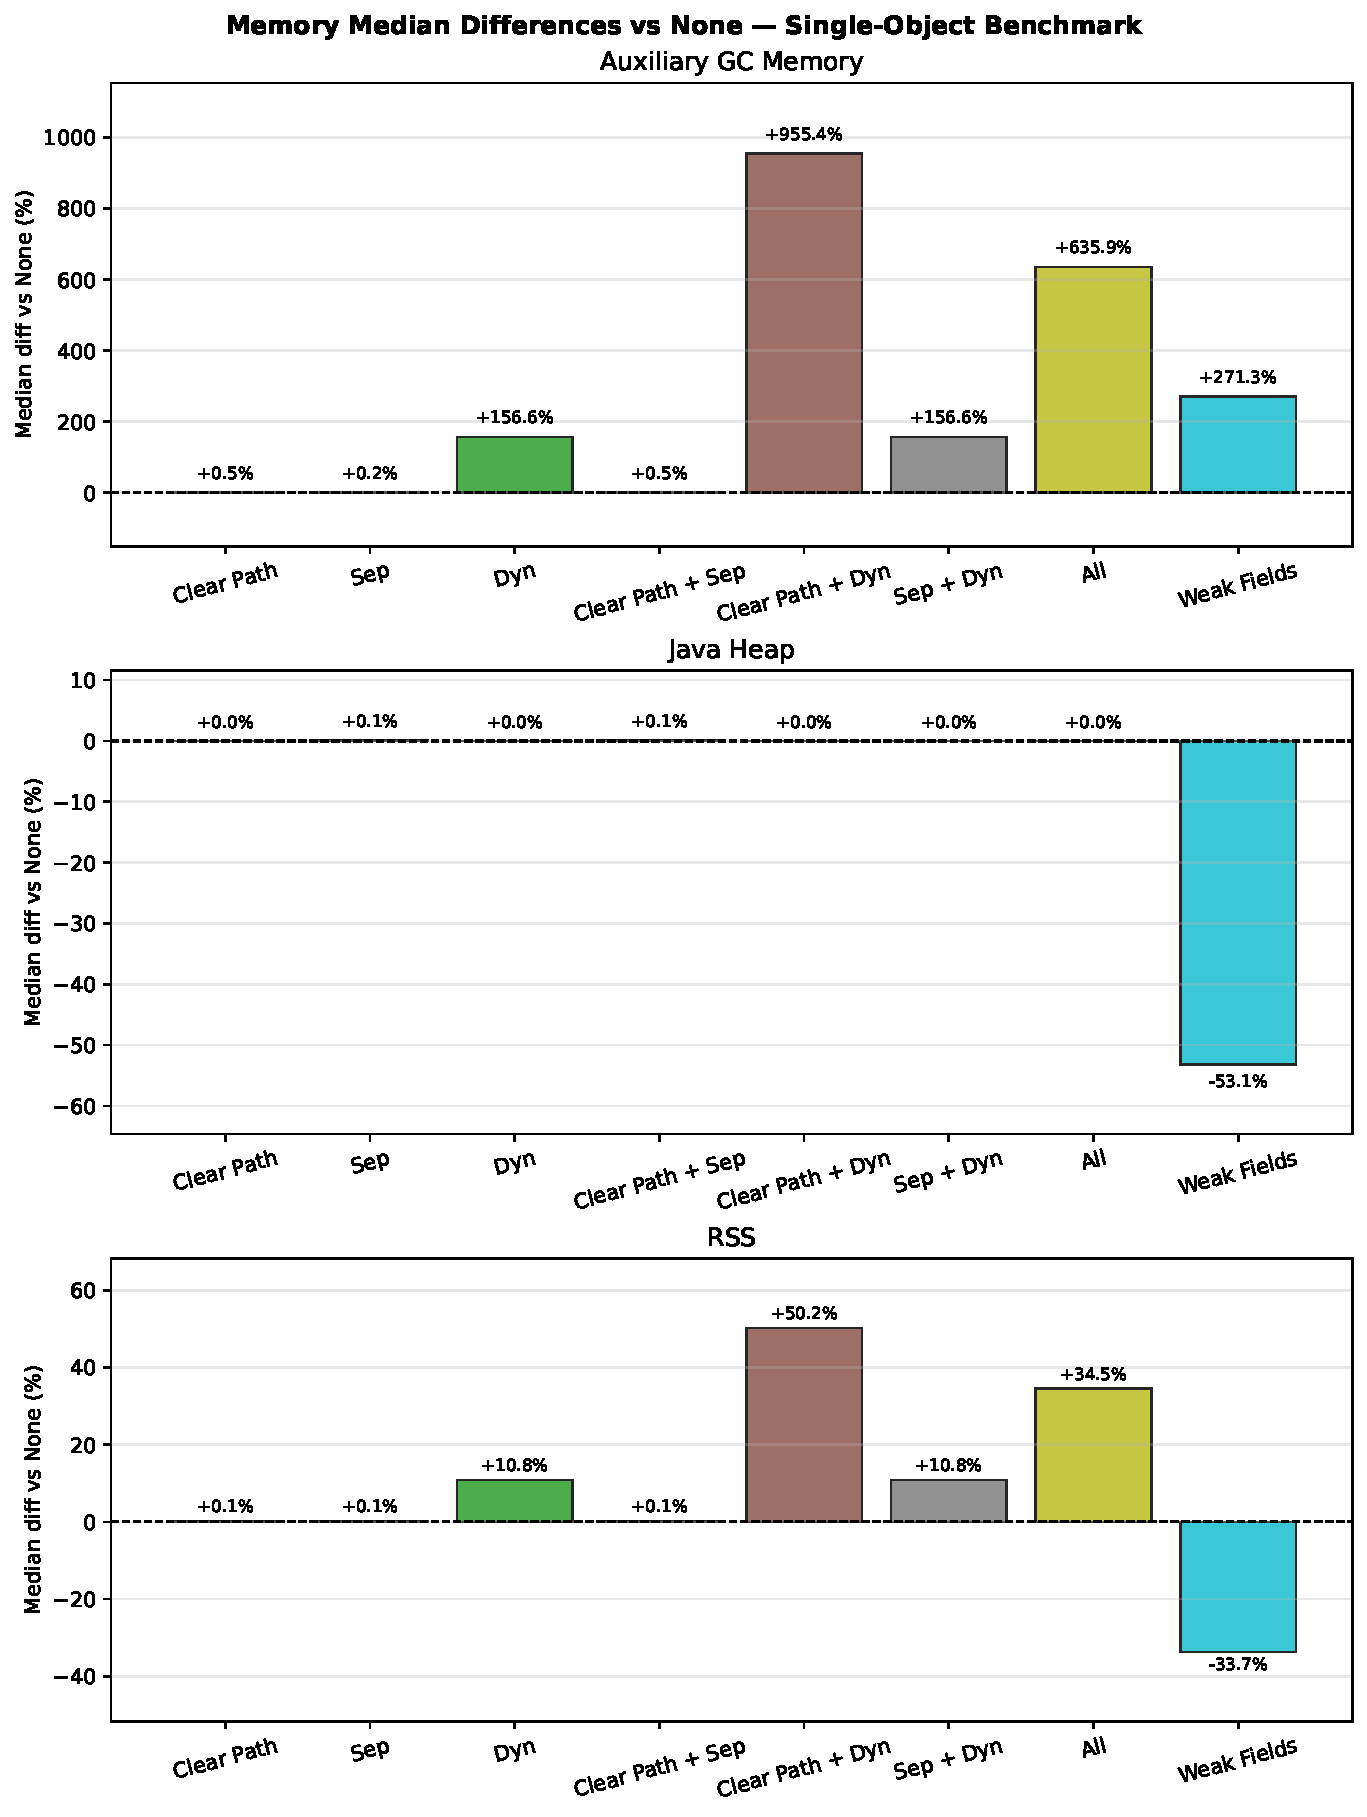
\includegraphics[width=\textwidth]{memory_median_diff_hist_slurm-5118807_combined_gc_single.pdf}
	\caption[Memory median percentage differences (single-object)]{Median percentage difference in per-run maximum memory usage relative to the \texttt{none} baseline, \DIFdelbeginFL \DIFdelFL{single-object benchmark}\DIFdelendFL \DIFaddbeginFL \textbf{\DIFaddFL{single-object benchmark}}\DIFaddendFL . Lower is better. Top to bottom: auxiliary \DIFdelbeginFL %DIFDELCMD < \ac{GC} %%%
\DIFdelendFL \DIFaddbeginFL \ac{GCr} \DIFaddendFL memory, Java heap, total process \ac{RSS}.}
	\label{fig:mem-single-hist}
\end{figure}

% ---------- Memory median diff histograms – multi ----------
\begin{figure}[t]
	\centering
	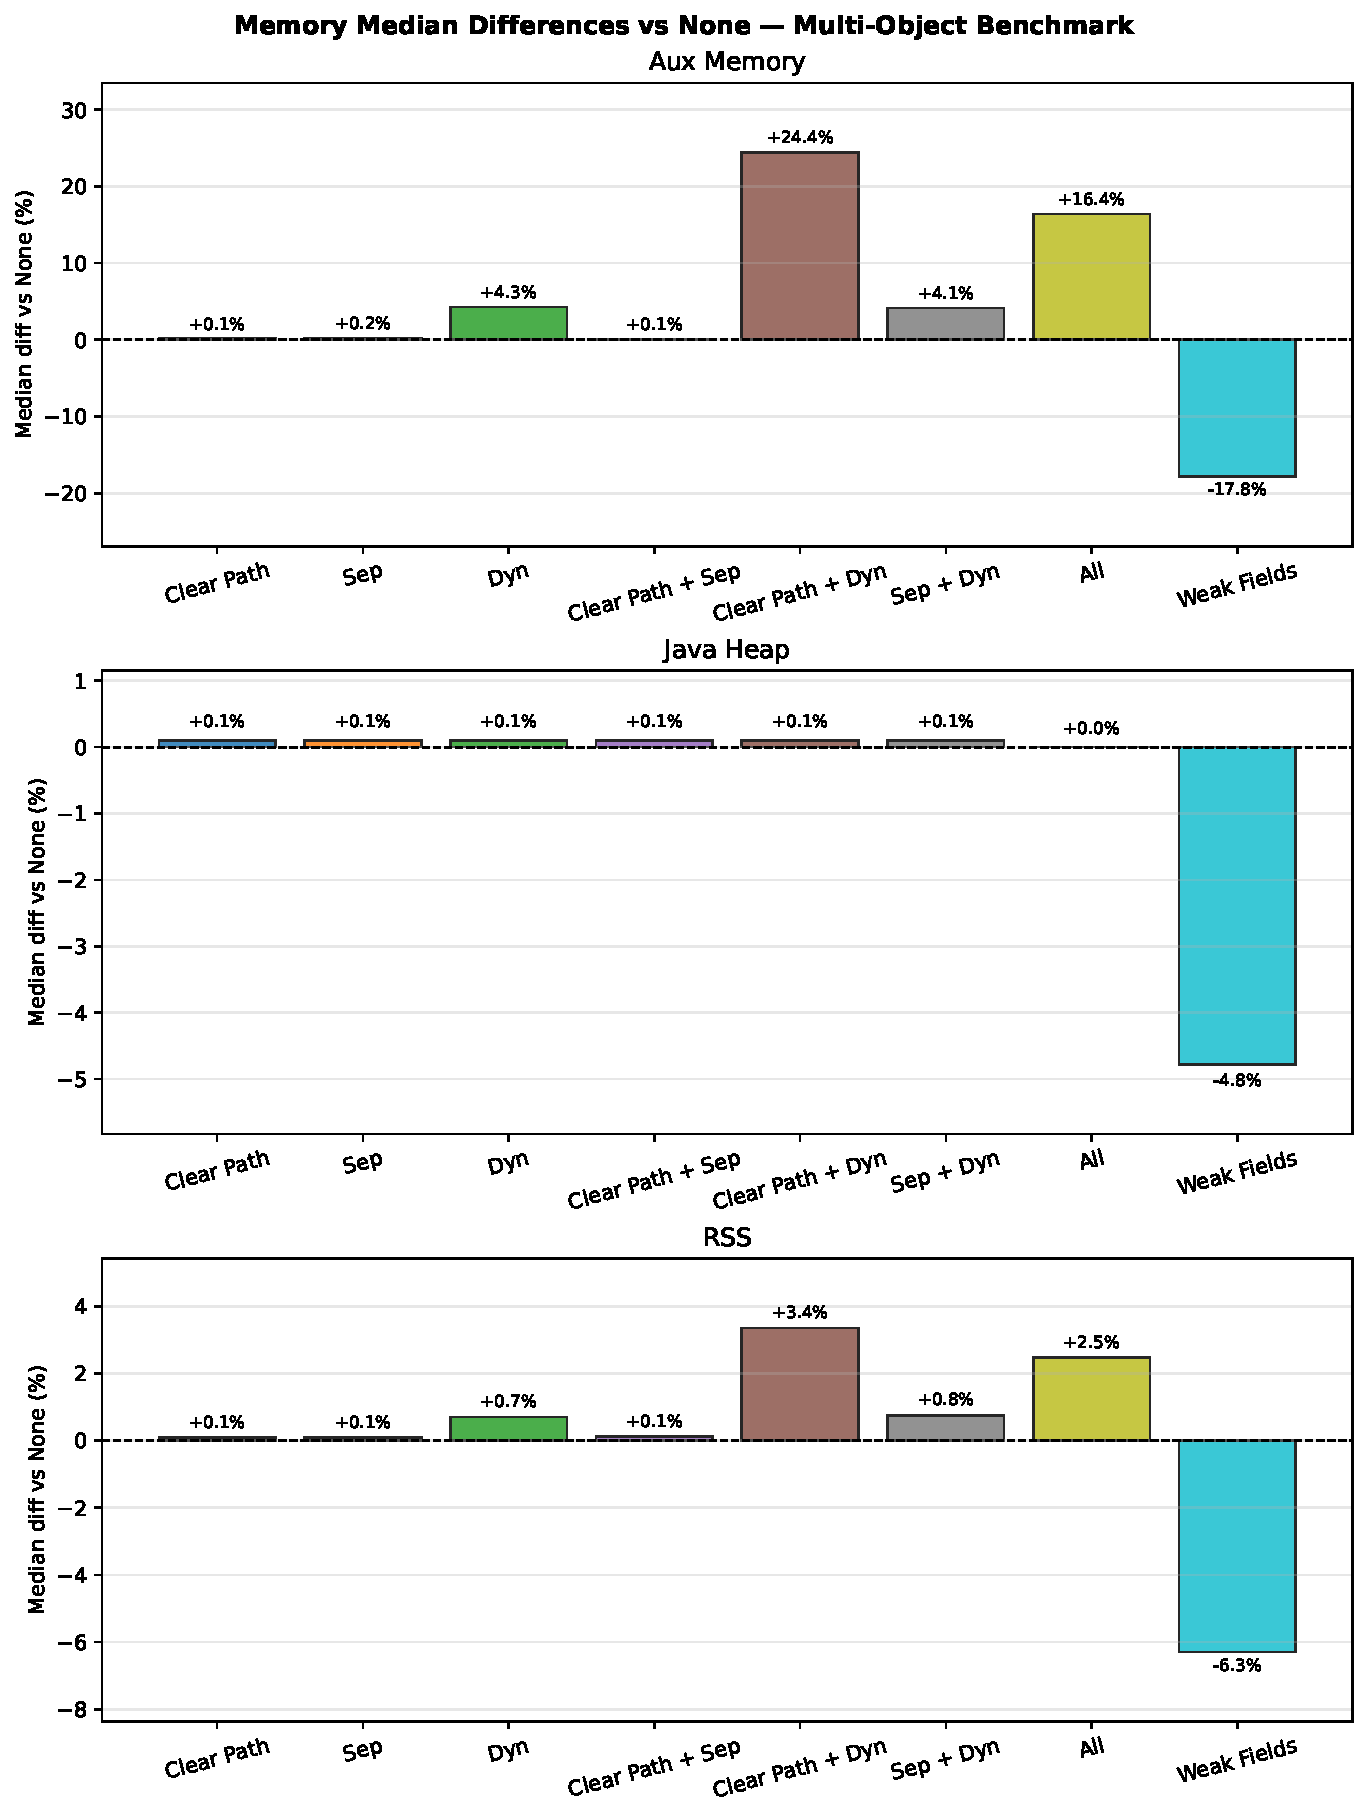
\includegraphics[width=\textwidth]{memory_median_diff_hist_slurm-5118807_combined_gc_multi.pdf}
	\caption[Memory median percentage differences (multi-object)]{Median percentage difference in per-run maximum memory usage relative to the \texttt{none} baseline, \DIFdelbeginFL \DIFdelFL{multi-object benchmark}\DIFdelendFL \DIFaddbeginFL \textbf{\DIFaddFL{multi-object benchmark}}\DIFaddendFL . Lower is better. Top to bottom: auxiliary \DIFdelbeginFL %DIFDELCMD < \ac{GC} %%%
\DIFdelendFL \DIFaddbeginFL \ac{GCr} \DIFaddendFL memory, Java heap, total process \ac{RSS}.}
	\label{fig:mem-multi-hist}
\end{figure}

  \fi
    \DIFdelbegin \DIFdel{\mbox{%DIFAUXCMD
\Cref{tab:nonstrong-fraction} }\hspace{0pt}%DIFAUXCMD
shows the fraction of median major-collection time attributable to non-strong processing for the }\texttt{\DIFdel{none}} %DIFAUXCMD
\DIFdel{baseline and the }\texttt{\DIFdel{all}} %DIFAUXCMD
\DIFdel{variant, across both benchmarks.
}%DIFDELCMD < 

%DIFDELCMD < \begin{table}[t]
%DIFDELCMD < \centering
%DIFDELCMD < %%%
%DIFDELCMD < \caption[Non-strong processing as a fraction of major-collection time]{%
{%DIFAUXCMD
\DIFdelFL{Median non-strong processing time and major-collection time for }\texttt{\DIFdelFL{none}} %DIFAUXCMD
\DIFdelFL{and }\texttt{\DIFdelFL{all}}%DIFAUXCMD
\DIFdelFL{, with the fraction of major-collection time attributable to non-strong processing.}}
%DIFAUXCMD
%DIFDELCMD < \label{tab:nonstrong-fraction}
%DIFDELCMD < \begin{tabular}{llrrr}
%DIFDELCMD < \toprule
%DIFDELCMD < %%%
\textbf{\DIFdelFL{Benchmark}} %DIFAUXCMD
%DIFDELCMD < & %%%
\textbf{\DIFdelFL{Variant}} %DIFAUXCMD
%DIFDELCMD < & %%%
\textbf{\DIFdelFL{Non-strong (ms)}} %DIFAUXCMD
%DIFDELCMD < & %%%
\textbf{\DIFdelFL{Major (ms)}} %DIFAUXCMD
%DIFDELCMD < & %%%
\textbf{\DIFdelFL{Fraction}} %DIFAUXCMD
%DIFDELCMD < \\
%DIFDELCMD < \midrule
%DIFDELCMD < %%%
\DIFdelFL{Single-object }%DIFDELCMD < & %%%
\texttt{\DIFdelFL{none}} %DIFAUXCMD
%DIFDELCMD < & %%%
\DIFdelFL{997  }%DIFDELCMD < & %%%
\DIFdelFL{6\,958 }%DIFDELCMD < & %%%
\DIFdelFL{14.3\,\% }%DIFDELCMD < \\
%DIFDELCMD < %%%
\DIFdelFL{Single-object }%DIFDELCMD < & %%%
\texttt{\DIFdelFL{all}}  %DIFAUXCMD
%DIFDELCMD < & %%%
\DIFdelFL{184  }%DIFDELCMD < & %%%
\DIFdelFL{6\,377 }%DIFDELCMD < & %%%
\DIFdelFL{2.9\,\%  }%DIFDELCMD < \\
%DIFDELCMD < %%%
\DIFdelFL{Multi-object  }%DIFDELCMD < & %%%
\texttt{\DIFdelFL{none}} %DIFAUXCMD
%DIFDELCMD < & %%%
\DIFdelFL{44.1 }%DIFDELCMD < & %%%
\DIFdelFL{982    }%DIFDELCMD < & %%%
\DIFdelFL{4.5\,\%  }%DIFDELCMD < \\
%DIFDELCMD < %%%
\DIFdelFL{Multi-object  }%DIFDELCMD < & %%%
\texttt{\DIFdelFL{all}}  %DIFAUXCMD
%DIFDELCMD < & %%%
\DIFdelFL{18.7 }%DIFDELCMD < & %%%
\DIFdelFL{970    }%DIFDELCMD < & %%%
\DIFdelFL{1.9\,\%  }%DIFDELCMD < \\
%DIFDELCMD < \bottomrule
%DIFDELCMD < \end{tabular}
%DIFDELCMD < \end{table}
%DIFDELCMD < 

%DIFDELCMD <     %%%
\DIFdelend \chapter{Analysis of Results}
\label{chap:analysis}

The measurements presented in \cref{sec:eval-results} show clear differences between configurations on some metrics and largely overlapping distributions on others. The analysis proceeds in two parts: a comparison among all variants on both the targeted non-strong processing metric and the broader collection-time metrics, followed by an analysis of memory usage and trade-offs. The \texttt{weak\_fields} variant is included throughout and compared with the \texttt{WeakReference} variants at each stage.

\section{Non-Strong Reference Processing}
\label{sec:analysis-nonstrong}

The metric most directly targeted by the implemented optimisations is \texttt{Concurrent Process Non-Strong}, which captures the total wall-clock time spent in \ac{ZGC}'s concurrent reference-processing phase per \ac{GC} cycle. This phase is the intended site of all three optimisations, and the clearest differences between variants are observed here, making it the natural starting point for the analysis.

Before comparing variants, it is worth establishing what fraction of total major-collection time is attributable to non-strong processing in the baseline. This fraction, summarised for the \texttt{none} baseline and the best-performing pipeline variant (\texttt{all}) in \DIFdelbegin \DIFdel{\mbox{%DIFAUXCMD
\cref{tab:nonstrong-fraction} }\hspace{0pt}%DIFAUXCMD
}\DIFdelend \DIFaddbegin \DIFadd{\mbox{%DIFAUXCMD
\cref{tab:stats-ratio-slurm-5118807_combined_gc} }\hspace{0pt}%DIFAUXCMD
}\DIFaddend in \cref{sec:eval-results}, represents the ceiling on how much the pipeline optimisations can reduce total major-collection time. Even an 81\,\% reduction in non-strong processing time can at most save the baseline fraction listed in that table. Realised savings in major-collection time will be smaller still because other phases are unaffected. The ceiling is much tighter in the multi-object benchmark: non-strong processing accounts for \DIFdelbegin \DIFdel{14.3}\DIFdelend \DIFaddbegin \DIFadd{14.7}\DIFaddend \,\% of major-collection time in the single-object \texttt{none} baseline but only 4.5\,\% in the multi-object \texttt{none} baseline, reflecting the more diverse workload in which \ac{GC} effort is spread across marking, relocation, and other phases. After applying all three optimisations (\texttt{all}), these fractions fall to \DIFdelbegin \DIFdel{2.9}\DIFdelend \DIFaddbegin \DIFadd{3}\DIFaddend \,\% and 1.9\,\% respectively.

\Cref{fig:gc-single-nonstrong,fig:gc-multi-nonstrong} show the distributions of this metric for the single-object and multi-object benchmarks respectively. Full numerical summaries are given in \cref{tab:stats-nonstrong}.

\subsection{Effect of the Clear Path and Dynamic Array}
\label{subsec:analysis-nonstrong-clear-dyn}

The most striking reduction is achieved by the \texttt{clear\_path\_dyn} variant. In the single-object benchmark its median non-strong processing time is 187.9\,ms, compared to 996.9\,ms for the unmodified \texttt{none} baseline, a reduction of approximately 81\,\%. The \texttt{all} variant, which adds the skip-enqueue separation on top of \texttt{clear\_path\_dyn}, reaches a nearly identical median of 184.4\,ms (also about an 81\,\% reduction). In the multi-object benchmark the pattern is consistent: \texttt{clear\_path\_dyn} achieves a median of 18.8\,ms versus 44.1\,ms for \texttt{none} (57\,\% reduction), and \texttt{all} reaches 18.7\,ms (also 57\,\% reduction).

The near-equivalence of \texttt{clear\_path\_dyn} and \texttt{all} shows that adding the skip-enqueue separation to a configuration that already has the dynamic array and the specialised clear path yields little extra benefit to reference processing times: \texttt{clear\_path\_dyn} and \texttt{all} differ by just 3.5\,ms in the single-object benchmark and 0.1\,ms in the multi-object benchmark.

The two individual optimisations \texttt{clear\_path\_only} and \texttt{dyn\_only} show that the dynamic array is the more impactful of the two but that both contribute meaningfully to the overall improvement when combined. The \texttt{clear\_path\_only} variant, which enables only the specialised clear path, reduces the single-object median by 7\,\% (to 923.7\,ms), while \texttt{dyn\_only}, which enables only the dynamic array, achieves a 36\,\% reduction (to 639.1\,ms). When combined in \texttt{clear\_path\_dyn}, the effect is substantially larger than either isolated contribution. This suggests that the dynamic-array traversal and the specialised clear logic remove different parts of the per-reference cost and therefore interact constructively rather than redundantly.

\subsection{Effect of the Skip-Enqueue Separation Alone}
\label{subsec:analysis-nonstrong-sep}

The \texttt{sep\_only} variant, which introduces the separate discovered list for queue-less weak references but does not include the dynamic array or the specialised clear path, produces negligible improvement on non-strong processing time. In the single-object benchmark its median is 943.8\,ms, only 5\,\% below the \texttt{none} baseline, and its IQR of 73.8\,ms is comparable to \texttt{none}'s 75.9\,ms. In the multi-object benchmark the difference is entirely eliminated: 44.1\,ms versus 44.1\,ms for \texttt{none}.

\subsection{Comparison with Weak Fields}
\label{subsec:analysis-nonstrong-wf}

The \texttt{weak\_fields} variant achieves a median non-strong processing time of 484.6\,ms in the single-object benchmark and 35.8\,ms in the multi-object benchmark. These figures correspond to reductions of 51\,\% and 19\,\% respectively relative to \texttt{none}, \DIFdelbegin \DIFdel{positioning }\texttt{\DIFdel{weak\_fields}} %DIFAUXCMD
\DIFdel{clearly above }\DIFdelend \DIFaddbegin \DIFadd{showing clear improvement over }\DIFaddend the \texttt{none} baseline \DIFdelbegin \DIFdel{but well below }\DIFdelend \DIFaddbegin \DIFadd{while remaining well short of }\DIFaddend the leading \texttt{clear\_path\_dyn} and \texttt{all} configurations. Its non-strong phase therefore improves clearly over the baseline, but not enough to match the best specialised \texttt{WeakReference} pipeline variants.

Notably, \texttt{weak\_fields} is closely comparable to \texttt{sep\_dyn} on this metric, especially in the multi-object benchmark where their medians are effectively indistinguishable: 35.8\,ms versus 35.5\,ms, a gap of just 0.3\,ms. Their distributions are also closely aligned, with \texttt{sep\_dyn} showing a slightly tighter \ac{IQR} of 7.1\,ms compared to \texttt{weak\_fields}'s 8.2\,ms. In the single-object benchmark \texttt{weak\_fields}'s median is somewhat lower (484.6\,ms versus 576.9\,ms for \texttt{sep\_dyn}, a difference of about 17\,\%) and \texttt{weak\_fields} has a substantially tighter IQR of 8.4\,ms compared to \texttt{sep\_dyn}'s 75.9\,ms. This suggests that the weak-field approach may have a slightly better and significantly more consistent performance profile when the reference load is extremely high as it is in the single-object benchmark.

\section{Overall \DIFdelbegin \DIFdel{GC }\DIFdelend \DIFaddbegin \DIFadd{GCr }\DIFaddend Collection Times}
\label{sec:analysis-overall}

In contrast to the non-strong processing metric, the overall collection time metrics show broad, heavily overlapping distributions across all \texttt{WeakReference} variants, making it difficult to draw firm conclusions from pairwise comparisons within this group. \texttt{weak\_fields}\DIFdelbegin \DIFdel{however }\DIFdelend \DIFaddbegin \DIFadd{, however, }\DIFaddend shows a clear difference in the distribution compared to all \texttt{WeakReference} variants across nearly all overall collection metrics.

\subsection{Major Collection}
\label{subsec:analysis-overall-weakref}

See \cref{fig:gc-single-major,fig:gc-multi-major} for the comparisons and \cref{tab:stats-major} for numerical summaries.

For the single-object benchmark, the median major collection time of \texttt{none} is 6\,958\,ms with an \ac{IQR} of about 1\,596\,ms. The \texttt{all} variant has a median of 6\,377\,ms (8\,\% below \texttt{none}) and the \texttt{clear\_path\_dyn} variant 6\,399\,ms (also 8\,\% below \texttt{none}), but with \acp{IQR} of 1\,419\,ms and 1\,394\,ms respectively, both distributions still overlap substantially with the baseline and with each other. Of the other \texttt{WeakReference} variants, \texttt{dyn\_only} has the lowest median at 6\,733\,ms, which is only about 3\,\% below \texttt{none}, while the rest of the variants have medians that are within about 1\,\% of \texttt{none} and \acp{IQR} that are comparable to \texttt{none}'s. In the multi-object benchmark the effect is even smaller in relative terms, with medians ranging from 965\,ms (\texttt{dyn\_only}) to 1\,002\,ms (\texttt{clear\_path\_sep}) against a baseline of 982\,ms, all distributions remain within a narrow \ac{IQR} band of roughly 93--136\,ms, making fine-grained ranking unreliable.

Among the \texttt{WeakReference} variants, \texttt{all} and \texttt{clear\_path\_dyn} tend to occupy the lower part of the collection-time distribution in both benchmarks, which is directionally consistent with their superior non-strong processing times. However, given the distribution overlap, this observation should be treated as \DIFdelbegin \DIFdel{indicative rather than conclusive}\DIFdelend \DIFaddbegin \DIFadd{slightly indicative}\DIFaddend .

The \texttt{weak\_fields} variant stands clearly apart on this metric. In the single-object benchmark its median major collection time is 4\,136\,ms, compared with 6\,377--7\,044\,ms for all \texttt{WeakReference} variants, a reduction of approximately 35\,\% against the best \texttt{WeakReference} variant and 41\,\% against \texttt{none}. Its IQR of 485\,ms is also substantially tighter than the 1\,354--1\,596\,ms \acp{IQR} of the \texttt{WeakReference} group. In the multi-object benchmark the gap is smaller but still unambiguous: 708\,ms versus 965--1\,002\,ms, a reduction of approximately 28\,\% versus \texttt{none}. The source of this advantage is structural: by eliminating the \texttt{WeakReference} objects entirely, \texttt{weak\_fields} reduces the amount of \DIFdelbegin \DIFdel{GC }\DIFdelend \DIFaddbegin \ac{GC} \DIFaddend work that must be performed across all phases of the cycle, not \DIFdelbegin \DIFdel{just }\DIFdelend \DIFaddbegin \DIFadd{only }\DIFaddend in the non-strong processing phase.

\subsection{Old Generation}
\label{subsec:analysis-overall-oldgen}

See \cref{fig:gc-single-old-gen,fig:gc-multi-old-gen} for the comparisons and \cref{tab:stats-oldgen} for full numerical summaries.

The old-generation collection time shows a clearer split among the \texttt{WeakReference} variants in the single-object benchmark than the major collection metric does. Configurations that include the dynamic array stand noticeably apart: \texttt{all} and \texttt{clear\_path\_dyn} both reach a median of approximately 2\,993--3\,003\,ms, roughly 17\,\% below the \texttt{none} baseline of 3\,631\,ms, while \texttt{dyn\_only} and \texttt{sep\_dyn} achieve intermediate reductions of around 7\,\% (3\,377\,ms and 3\,393\,ms respectively). By contrast, the non-dynamic-array variants (\texttt{sep\_only}, \texttt{clear\_path\_only}, \texttt{clear\_path\_sep}) remain within 1\,\% of \texttt{none} at 3\,600--3\,676\,ms. Given that the \acp{IQR} are 600--720\,ms for the dynamic-array variants and 600--870\,ms for the non-dynamic variants, the distributions of the two groups do overlap, nevertheless, the median separation of roughly 600\,ms between \texttt{all} and the non-dynamic cluster is comparable to a full IQR, indicating a consistent directional effect. In the multi-object benchmark the picture is completely different: all \texttt{WeakReference} variants fall within 792--831\,ms against a baseline of 809\,ms.

The \texttt{weak\_fields} variant again reduces the median substantially: 2\,295\,ms in the single-object benchmark (37\,\% below \texttt{none}'s 3\,631\,ms) and 554\,ms in the multi-object benchmark (31\,\% below \texttt{none}'s 809\,ms). Its IQR of 282\,ms in the single-object benchmark is also considerably tighter than the 600--870\,ms range of the \texttt{WeakReference} group. As stated in \cref{subsec:analysis-overall-weakref}, this advantage is attributable to the reduced \DIFdelbegin \DIFdel{GC }\DIFdelend \DIFaddbegin \ac{GC} \DIFaddend workload across all phases of the cycle, not \DIFdelbegin \DIFdel{just }\DIFdelend \DIFaddbegin \DIFadd{only }\DIFaddend the non-strong processing phase.



\subsection{Old Phase: Concurrent Mark}
\label{subsec:analysis-overall-mark}

See \cref{fig:gc-single-old-mark,fig:gc-multi-old-mark} for the comparisons and \cref{tab:stats-old-concurrent-mark} for numerical summaries.

The concurrent mark phase shows where the \texttt{WeakReference} pipeline optimisations suffer. In the single-object benchmark, \texttt{WeakReference} variant medians for the old-phase concurrent mark metric fall in the range 2\,575--2\,780\,ms, with \texttt{none} at 2\,575\,ms. The combination variants with dynamic arrays show higher medians (\texttt{clear\_path\_dyn} at 2\,780\,ms, \texttt{all} at 2\,750\,ms), the \texttt{dyn\_only} variant is slightly lower at 2\,644\,ms, which is expected given that less information is stored in the dynamic array entries. However, this pattern is not consistent across benchmarks: in the multi-object benchmark, for example, the \texttt{dyn\_only} variant has a median of 570\,ms, which is \DIFdelbegin \DIFdel{actually }\DIFdelend lower than the \texttt{none} median of 578\,ms. Due to the high \acp{IQR} (560--810\,ms and 67--99\,ms respectively) the differences observed between the \texttt{WeakReference} variants on this metric should \DIFaddbegin \DIFadd{also }\DIFaddend be treated as \DIFdelbegin \DIFdel{indicative rather than conclusive}\DIFdelend \DIFaddbegin \DIFadd{slightly indicative}\DIFaddend .

In contrast, \texttt{weak\_fields} reduces the concurrent mark median by approximately 31\,\% in both benchmarks (1\,782\,ms in single-object, versus 2\,575\,ms for \texttt{none}\DIFdelbegin \DIFdel{, }\DIFdelend \DIFaddbegin \DIFadd{; }\DIFaddend 399\,ms versus 578\,ms in the multi-object benchmark). This is again consistent with the statements above: \DIFaddbegin \DIFadd{by }\DIFaddend eliminating the \texttt{WeakReference} objects, \texttt{weak\_fields} reduces the amount of \DIFdelbegin \DIFdel{GC }\DIFdelend \DIFaddbegin \ac{GC} \DIFaddend work that must be performed across most phases of the cycle, including concurrent marking.

\subsection{Young Generation (Promote All)}
\label{subsec:analysis-overall-younggen}

See \cref{fig:gc-single-young-gen,fig:gc-multi-young-gen} for the comparisons and \cref{tab:stats-young-gen} for numerical summaries.

The young-generation (Promote All) phase shows no systematic response to the \texttt{WeakReference} pipeline optimisations, as expected: all three optimisations operate exclusively on old-generation reference processing and should have no bearing on young-generation work. The majority of \texttt{WeakReference} variants in both benchmarks fall within $\pm$1.5\,\% of the \texttt{none} median (3\,201\,ms in the single-object benchmark, 164\,ms in the multi-object benchmark). Two isolated deviations stand out but are unlikely to reflect genuine causal effects: neither replicates across both benchmarks, and each falls well within the natural spread of its own distribution. In the single-object benchmark, \texttt{sep\_dyn} has a median of 3\,439\,ms, some 7.4\,\% above \texttt{none}, yet this deviation is well within its IQR of 1\,622\,ms and disappears entirely in the multi-object benchmark where \texttt{sep\_dyn} is within 0.3\,\% of baseline. In the multi-object benchmark, \texttt{dyn\_only} has a median of 156\,ms, 4.8\,\% below the \texttt{none} median of 164\,ms\DIFdelbegin \DIFdel{, this }\DIFdelend \DIFaddbegin \DIFadd{. This }\DIFaddend too sits within its IQR of 45\,ms and has no counterpart in the single-object benchmark where \texttt{dyn\_only} is within 1\,\% of baseline.

The \texttt{weak\_fields} variant again stands apart: a $-$44\,\% reduction in the single-object benchmark and $-$16\,\% in the multi-object benchmark, attributable to the elimination of \texttt{WeakReference} objects that would otherwise be marked and then promoted (moved to the old generation).

\section{Memory Behaviour}
\label{sec:analysis-memory}

The dynamic-array optimisation improves non-strong processing time at the cost of allocating a contiguous buffer per \ac{GC} worker thread rather than reusing the intrusive linked-list fields already present in \texttt{Reference} objects. This trade-off makes memory usage an important secondary dimension of the evaluation \DIFdelbegin \DIFdel{. Auxiliary }%DIFDELCMD < \ac{GC} %%%
\DIFdelend \DIFaddbegin \DIFadd{and since the dynamic array is allocated by the }\ac{GCr}\DIFadd{, the auxiliary }\ac{GCr} \DIFaddend memory is the most direct indicator of the dynamic array's overhead\DIFdelbegin \DIFdel{, since the array allocates a contiguous buffer per }%DIFDELCMD < \ac{GC} %%%
\DIFdel{worker thread rather than reusing the existing fields of }\texttt{\DIFdel{Reference}} %DIFAUXCMD
\DIFdel{objects}\DIFdelend . Java heap occupancy reflects the cost of maintaining the \texttt{WeakReference} objects themselves, which \texttt{weak\_fields} eliminates entirely. Total process \ac{RSS} captures the combined footprint of heap, \DIFdelbegin %DIFDELCMD < \ac{GC} %%%
\DIFdelend \DIFaddbegin \ac{GCr} \DIFaddend metadata, and native memory, providing the broadest view of the memory trade-off. See \Cref{fig:mem-single-hist,fig:mem-multi-hist} for the comparisons and \cref{tab:stats-memory-aux,tab:stats-memory-java-heap,tab:stats-memory-rss} for numerical summaries.

\subsection{Auxiliary \DIFaddbegin \DIFadd{GCr }\DIFaddend Memory Usage and the Dynamic Array}
\label{subsec:analysis-memory-aux}

All configurations that include the dynamic array (\texttt{dyn\_only}, \texttt{sep\_dyn}, \texttt{clear\_path\_dyn}, and \texttt{all}) incur substantially higher auxiliary \DIFaddbegin \ac{GCr} \DIFaddend memory than variants that retain the intrusive linked list. In the single-object benchmark, the median per-run maximum for \texttt{dyn\_only} and \texttt{sep\_dyn} is 308\,MB of \DIFdelbegin %DIFDELCMD < \ac{GC}%%%
\DIFdel{-committed }\DIFdelend \DIFaddbegin \DIFadd{auxiliary }\ac{GCr} \DIFaddend memory, compared to approximately 120\,MB for the linked-list variants, an increase of 157\,\%. The \texttt{clear\_path\_dyn} variant is the highest of all at 1\,268\,MB (roughly 10$\times$ the non-array baseline), and \texttt{all} reaches 884\,MB (+637\,\%). In the multi-object benchmark the relative differences are much smaller: \texttt{dyn\_only} and \texttt{sep\_dyn} are only 4\,\% above the \texttt{none} baseline of 292\,MB at 305\,MB and 304\,MB respectively, \texttt{all} is 340\,MB (+16\,\%), and \texttt{clear\_path\_dyn} is 363\,MB (+24\,\%).

The \texttt{weak\_fields} variant occupies an intermediate position. Its median auxiliary \DIFaddbegin \ac{GCr} \DIFaddend memory in the single-object benchmark is 446\,MB, 272\,\% above the 120\,MB of the non-array \texttt{WeakReference} variants but well below \texttt{clear\_path\_dyn}'s 1\,268\,MB. In the multi-object benchmark it is the lowest of all configurations at 240\,MB, 18\,\% below the \texttt{none} baseline of 292\,MB.

\subsection{Java Heap Usage}
\label{subsec:analysis-memory-heap}

The heap usage figures are essentially identical across all \texttt{WeakReference} variants (approximately 1\,720\,MB per-run median in the single-object benchmark and 1\,926--1\,928\,MB in the multi-object benchmark), with all variants within 0.1\,\% of each other.

The \texttt{weak\_fields} variant, however, shows markedly lower heap usage: a median of 806\,MB in the single-object benchmark, 53\,\% below the \texttt{WeakReference} group, and 1\,834\,MB in the multi-object benchmark, 5\,\% below. This is consistent with the fact that \texttt{weak\_fields} eliminates the \texttt{WeakReference} objects entirely, which constitute a significant portion of the heap occupancy in the \texttt{WeakReference} variants.

\subsection{Process Memory Footprint}
\label{subsec:analysis-memory-rss}

The \ac{RSS} results follow the same overall direction as auxiliary \DIFaddbegin \ac{GCr} \DIFaddend memory and heap usage. In the single-object benchmark, \texttt{clear\_path\_dyn} reaches the highest median \ac{RSS} at 2\,856\,MB (+50\,\% versus the \texttt{none} baseline of 1\,901\,MB), followed by \texttt{all} at 2\,556\,MB (+34\,\%) and \texttt{dyn\_only} and \texttt{sep\_dyn} at 2\,107\,MB each (+11\,\%). The non-array \texttt{WeakReference} variants remain within 0.2\,\% of \texttt{none}. \texttt{weak\_fields}, by contrast, has the lowest median RSS of all configurations at 1\,260\,MB, 34\,\% below \texttt{none}. In the multi-object benchmark the spread is much narrower: \texttt{clear\_path\_dyn} is the highest at 2\,487\,MB (+3\,\% versus \texttt{none}'s 2\,407\,MB), while \texttt{weak\_fields} is the lowest at 2\,255\,MB (−6\,\%). This strengthens the interpretation that the dynamic-array variants trade runtime memory overhead for faster queue-less weak-reference processing, while weak fields reduce both heap occupancy and total process footprint.

    \chapter{Discussion}
\label{chap:discussion}

Across both benchmarks, the pipeline optimisations improve the metrics they directly target while leaving broader collection behaviour relatively unchanged. \DIFdelbegin \DIFdel{From this result }\DIFdelend \DIFaddbegin \DIFadd{Against this backdrop, }\DIFaddend the \texttt{weak\_fields} variant stands apart: by eliminating \texttt{WeakReference} objects from the heap entirely, it propagates improvements through every phase of the collection cycle rather than \DIFdelbegin \DIFdel{just }\DIFdelend \DIFaddbegin \DIFadd{only }\DIFaddend the reference processing phase. The following sections explain the mechanisms behind these patterns and reflect on the scope of the evaluation.

\section{Superadditive Interaction of the Clear Path and Dynamic Array}
\label{sec:disc-synergy}

One clear result in reference processing times is that \DIFaddbegin \DIFadd{the }\texttt{\DIFadd{clear\_path\_dyn}} \DIFadd{variant, }\DIFaddend combining the clear-path optimisation with the dynamic array\DIFaddbegin \DIFadd{, }\DIFaddend produces an 81\,\% reduction in non-strong processing time, far larger than the sum of their individual contributions (7\,\% and 36\,\% respectively). This superadditivity arises from the tight coupling of the two mechanisms at the implementation level.

In \texttt{dyn\_only}, the dynamic array provides improved cache locality during traversal: discovered references are stored contiguously in memory, so iterating through them involves sequential cache-line loads rather than following pointer chains scattered across the heap~\cite{drepper07-memory}. However, the per-reference processing logic still uses the standard \ac{CAS}-based clear path, including a load barrier on the referent field and a \ac{CAS} operation to atomically set the cleared referent to a coloured null pointer. These operations are not eliminated by the array alone.

In \texttt{clear\_path\_only}, the specialised clear logic eliminates the \ac{CAS} on the referent field for old-generation referents (replacing it with a direct store) and removes the virtual call to determine the reference type. However, the referent field address and value must still be loaded individually for each reference during processing, and traversal still follows the intrusive linked list with its associated cache misses.

When both optimisations are active in \texttt{clear\_path\_dyn}, the dynamic array enables a further key capability: the referent field address and value are pre-loaded during discovery and stored directly in the array entry (see \cref{lst:dynamic-array-processing}). In processing\DIFdelbegin \DIFdel{these values get }\DIFdelend \DIFaddbegin \DIFadd{, these values are }\DIFaddend read from the contiguous array without issuing any additional heap loads. The specialised clear path operates on the pre-loaded data, removing both the load-barrier overhead and the pointer-chasing overhead simultaneously. In summary, each optimisation seems to remove a bottleneck that would persist if the other were applied alone.

\section{Skip-Enqueue Separation Providing Minimal Benefit}
\label{sec:disc-sep}

The skip-enqueue optimisation was motivated by the observation that the enqueueing stage performed unnecessary work for queue-less weak references: the references were still linked into the pending list, transferred to the \texttt{ReferenceHandler} thread, and iterated over only to be discarded~\cite{openjdk-reference-java,openjdk-zreferenceprocessor-cpp,JDK-8029205}. Despite this, \texttt{sep\_only} reduces the single-object median by only 5\,\% and shows no reduction in the multi-object benchmark. When combined with the dynamic array in \texttt{sep\_dyn}, the improvement over \texttt{dyn\_only} is only 6 \DIFdelbegin \DIFdel{\,pp }\DIFdelend \DIFaddbegin \DIFadd{percentage points }\DIFaddend in the single-object benchmark and 2 \DIFdelbegin \DIFdel{\,pp }\DIFdelend \DIFaddbegin \DIFadd{percentage points }\DIFaddend in the multi-object benchmark. The same pattern continues in the \texttt{all} variant, which \DIFdelbegin \DIFdel{only sees an increase of }\DIFdelend \DIFaddbegin \DIFadd{shows only a }\DIFaddend 0.3 \DIFdelbegin \DIFdel{\,pp }\DIFdelend \DIFaddbegin \DIFadd{percentage point increase }\DIFaddend over \texttt{clear\_path\_dyn} in the single-object benchmark and a 0.2 \DIFdelbegin \DIFdel{\,pp }\DIFdelend \DIFaddbegin \DIFadd{percentage point }\DIFaddend increase in the multi-object benchmark. Where \texttt{all} offers a meaningful advantage over \texttt{clear\_path\_dyn} is in auxiliary \DIFdelbegin %DIFDELCMD < \ac{GC} %%%
\DIFdelend \DIFaddbegin \ac{GCr} \DIFaddend memory: by routing queue-less references to the separate list, the array entries in \texttt{all} do not need to store the reference address field that \texttt{clear\_path\_dyn} requires, reducing auxiliary \DIFaddbegin \ac{GCr} \DIFaddend memory by approximately 30\DIFaddbegin \DIFadd{\,}\DIFaddend \% in the single-object benchmark (from 1\,268\,MB to 884\,MB).

This likely means that the enqueue stage was not the bottleneck in reference processing in these benchmarks. The dominant costs in the pipeline appear to lie in the processing stage.

However, \DIFdelbegin \DIFdel{something not tested for in }\DIFdelend \DIFaddbegin \DIFadd{one effect not captured by }\DIFaddend the evaluation is that the skip-enqueue separation should reduce the load on the \texttt{ReferenceHandler} thread, which must process the pending list and perform callbacks for queue-backed references. By routing queue-less references away from this thread, the separation should reduce contention and improve latency for queue-backed references in a mixed workload. \DIFaddbegin \DIFadd{This is a plausible benefit of the mechanism, but it remains a hypothesis: neither benchmark in the evaluation contains queue-backed references, so this effect cannot be confirmed from the collected data.
}\DIFaddend 

\section{Concurrent-Mark \DIFdelbegin \DIFdel{Regression}\DIFdelend \DIFaddbegin \DIFadd{Impact}\DIFaddend }
\label{sec:disc-mark}

In the single-object benchmark, variants with the dynamic array show slightly higher concurrent-mark times than \texttt{none}: \texttt{dyn\_only} is 3\,\% higher, \texttt{clear\_path\_dyn} is 8\,\% higher, \texttt{sep\_dyn} is 6\,\% higher, and \texttt{all} is 7\,\% higher. This pattern is not observed in the multi-object benchmark, where concurrent-mark times are either unchanged, slightly lower, or slightly higher without a clear pattern.

There are two plausible explanations for the single-object \DIFdelbegin \DIFdel{regression}\DIFdelend \DIFaddbegin \DIFadd{increase}\DIFaddend . First, the dynamic array variants manage a large auxiliary data structure (the \texttt{ZWeakRefArray}) during \ac{GC} cycles, which increases memory pressure during the concurrent mark phase. Second, the dynamic array variants may have slightly higher average per-reference processing times during marking due to the additional logic for growing and copying the array. However, the fact that the \DIFdelbegin \DIFdel{regression }\DIFdelend \DIFaddbegin \DIFadd{increase }\DIFaddend is not observed in the multi-object benchmark, where the reference population is smaller and the processing workload is spread across multiple cycles, suggests that the additional per-reference processing time is the primary cause. Since the processing workload is spread over multiple cycles and no extra references are created, the auxiliary array only has to grow in the mark phase of the first cycle. In subsequent cycles, the array can be reused without growth thanks to the capacity reservation strategy (see \cref{subsec:di-dyn-impl}). This means that the usage of the auxiliary array seems to incur a per-reference processing overhead, but only when encountering new references that exceed the previously reserved capacity.

\section{Memory Overhead of the Pre-Loaded Array Entries}
\label{sec:disc-mem}

The auxiliary \DIFdelbegin %DIFDELCMD < \ac{GC} %%%
\DIFdelend \DIFaddbegin \ac{GCr} \DIFaddend memory results show a notable asymmetry among the dynamic-array variants: \texttt{dyn\_only} and \texttt{sep\_dyn} use 308\,MB in the single-object benchmark (157\,\% above \texttt{none}'s 120\,MB), while \texttt{clear\_path\_dyn} uses 1\,268\,MB (roughly 10$\times$ the non-array baseline) and \texttt{all} uses 884\,MB. This asymmetry directly reflects the per-entry struct size.

The \texttt{ZWeakRefArray} used in \texttt{dyn\_only} stores one entry per discovered reference containing the reference's address, which is required for processing. The \texttt{clear\_path\_dyn} variant uses an extended entry that additionally stores pre-loaded values enabling the barrier-free clear path described in \cref{sec:di-clear}. The discrepancy between \texttt{clear\_path\_dyn} and \texttt{all} is explained by the implementation, where \texttt{all} does not require the reference address since that is only needed for other reference types, but it does still require the pre-loaded values for the clear path.

In the multi-object benchmark, the same pattern holds but the absolute differences are smaller since the reference population is smaller.

One interesting observation is that the \texttt{weak\_fields} variant also follows this pattern in the single-object benchmark, using 446\,MB of auxiliary \DIFdelbegin %DIFDELCMD < \ac{GC} %%%
\DIFdelend \DIFaddbegin \ac{GCr} \DIFaddend memory (271\,\% above \texttt{none}'s 120\,MB) but not in the multi-object benchmark, where it uses 240\,MB (18\,\% below \texttt{none}'s 292\,MB). This is odd since the \texttt{weak\_fields} variant should follow the pattern in both cases \DIFdelbegin \DIFdel{, as }\DIFdelend \DIFaddbegin \DIFadd{since }\DIFaddend it is also backed by a dynamic array (\texttt{WeakFieldArray})\DIFdelbegin \DIFdel{; }\DIFdelend \DIFaddbegin \DIFadd{, }\DIFaddend why it has a below-baseline auxiliary \DIFaddbegin \ac{GCr} \DIFaddend memory usage in the multi-object benchmark is unclear. The most likely explanation is that the \texttt{weak\_fields} variant's reduced number of objects on the heap leads to some reduction in the auxiliary \DIFaddbegin \ac{GCr} \DIFaddend memory used for other \DIFdelbegin \DIFdel{GC }\DIFdelend \DIFaddbegin \ac{GCr} \DIFaddend data structures, which is enough to offset the additional memory used by the \texttt{WeakFieldArray} in the multi-object benchmark but not in the single-object benchmark where the reference population is larger and the auxiliary array is larger.

\section{Structural Advantage of Weak Fields}
\label{sec:disc-wf}

The \texttt{weak\_fields} variant achieves improvements across all measured \ac{GC} metrics because its advantage is structural rather than algorithmic: eliminating the \texttt{WeakReference} wrapper objects reduces the number of live objects the \ac{GCr} must process in every phase of the collection cycle, not just in reference processing.

In the single-object benchmark, 20 million \texttt{WeakReference} objects are heap-allocated Java objects. Each such object must be individually processed during each phase of each \ac{GC} cycle. In contrast, the \texttt{weak\_fields} variant eliminates these objects entirely, so the \ac{GCr} only processes the holder objects and the referents, which are already present in the heap for the Java application. This leads to a reduction in \ac{GC} workload across the board, from marking to compaction, and from young generation to old generation.

The heap usage data confirms the claim that there are fewer objects allocated: \texttt{weak\_fields} uses 806\,MB versus 1\,720\,MB for all \texttt{WeakReference} variants in the single-object benchmark (53\,\% lower). In the multi-object benchmark the absolute effect is smaller because the 2 million references represent a smaller fraction of total heap activity, from 1\,926\,MB to 1\,834\,MB, a 5\,\% reduction.

\section{Processing Mechanics of Weak Fields}
\label{sec:disc-wf-residual}

On the processing side, \texttt{weak\_fields} is mechanically similar to \texttt{sep\_dyn}. Entries discovered during old-generation marking are stored in a per-worker \texttt{ZWeakFieldArray}, the direct analogue of the \texttt{ZWeakRefArray} used by the dynamic-array \texttt{WeakReference} variants. Like queue-less \texttt{WeakReference} objects in \texttt{sep\_dyn}, weak-field entries carry no \texttt{ReferenceQueue} and therefore bypass the enqueue stage entirely: once the referent is found to be unreachable, the annotated field is zeroed without creating a pending-list entry. Due to the fields being writable, the \ac{CAS}-based clear path is required to ensure that the field is not changed to an incorrect value. This is analogous to the clear path for queue-less \texttt{WeakReference} objects in both \texttt{dyn\_only} and \texttt{sep\_dyn}, neither of which employs the optimised clear path.

This structural parallel is reflected in the non-strong processing times. \texttt{weak\_fields} achieves a 51\,\% reduction in the single-object benchmark, compared to \texttt{sep\_dyn}'s 42\,\% and \texttt{dyn\_only}'s 36\,\%. The somewhat better figure for \texttt{weak\_fields} is consistent with the simpler per-entry structure: annotated fields are stored and cleared directly, without the \texttt{WeakReference} object header, queue field, next field, and discovered field.

The result does not reach the 81\,\% reductions of \texttt{clear\_path\_dyn} and \texttt{all} for the reason mentioned previously: the clear path for weak fields cannot be optimised in the same way as for queue-less \texttt{WeakReference} objects, so the per-entry processing logic still involves a \ac{CAS} operation, which is not the case for \texttt{clear\_path\_dyn} and \texttt{all}.

\section{Limitations}
\label{sec:disc-limits}

Several aspects of the evaluation warrant care in interpreting the results.

\textbf{Benchmark representativeness.} Both benchmarks are custom and synthetic microbenchmarks designed to isolate reference processing overhead. The single-object benchmark concentrates its entire weak-reference load into a single \ac{GC} cycle, and the multi-object benchmark uses a fixed reference population with a regular promotion pattern. Neither benchmark captures the full diversity of real-world weak-reference usage, such as dynamic cache eviction, concurrent insertion and removal, or workloads with a mixture of queue-backed and queue-less references. The strong improvements observed on the non-strong processing metric may therefore represent an upper bound on what would be seen in a more heterogeneous production workload. \DIFaddbegin \DIFadd{Evaluating the variants on a real-world application benchmark would require either instrumenting an existing application or identifying a suitable open-source workload with measurable weak-reference usage. Java Flight Recorder (}\acs{JFR}\DIFadd{) could assist such an evaluation by providing per-event }\ac{GC} \DIFadd{timing data at low overhead, enabling the collection of the same metrics used here without requiring custom benchmark instrumentation. Ensuring measurement validity would also require monitoring system load throughout the run, to detect interference from competing processes on shared infrastructure.
}\DIFaddend 

\textbf{Single hardware platform.} All measurements were collected on a single \ac{UPPMAX} cluster configuration (see \cref{subsec:eval-env}). The results may not generalise to different \ac{CPU} micro-architectures, \ac{NUMA} configurations, or cache hierarchy sizes.

\textbf{ReferenceHandler thread \ac{CPU} time.} Neither benchmark contains queue-backed references, so the \texttt{ReferenceHandler} thread had no pending-list entries to process regardless of variant. Its \ac{CPU} usage was therefore not captured by any of the collected \ac{GC} metrics. This means the full benefit of the skip-enqueue separation in a workload with a mixture of queue-backed and queue-less references cannot be quantified from the current data.

\textbf{Correctness coverage.} The correctness of the implementation was verified through the standard OpenJDK test suite and manual inspection, not through formal verification or an exhaustive stress suite for the weak-field annotation. In particular, since the OpenJDK test suite does not include any tests for the \texttt{@weak} annotation, the correctness of the \texttt{weak\_fields} variant relies on the soundness of the implementation and the absence of crashes or assertion failures during the benchmark runs.



    \chapter{Related Work}
\label{chap:related-work}

\DIFdelbegin \DIFdel{Directly published work on optimising }\DIFdelend \DIFaddbegin \DIFadd{The preceding chapters have established that, in the evaluated setting, the structural choice of whether to represent weak references through dedicated wrapper objects or through annotated fields has a larger impact on }\ac{GC} \DIFadd{cost than pipeline-level optimisations. This chapter situates that finding within a broader design space by surveying how other language runtimes approach the same problem: providing weak reachability without preventing collection. The survey reveals recurrent design patterns, including a near-universal separation of weak reachability from cleanup notification, and a preference for probe-based semantics over callback-based notification in most mainstream systems. These cross-language comparisons provide context for understanding why Java's coupled }\texttt{\DIFadd{WeakReference}} \DIFadd{model is comparatively expensive for probe-only workloads, and for assessing where the weak-field mechanism explored in this thesis sits within the space of known alternatives.
}

\DIFadd{Published work directly addressing the optimisation of }\DIFaddend \ac{ZGC}'s weak-reference pipeline is limited\DIFdelbegin \DIFdel{, }\DIFdelend \DIFaddbegin \DIFadd{; }\DIFaddend the closest relevant material is therefore a combination of runtime documentation, implementation sources, and cross-language designs for weak semantics.
\DIFdelbegin \DIFdel{This chapter positions the thesis against those adjacent designs.
}\DIFdelend 

\section{Java and the \DIFdelbegin %DIFDELCMD < \ac{JVM}%%%
\DIFdelend \DIFaddbegin \DIFadd{JVM}\DIFaddend }
\label{sec:rw-java}

Java's reference \ac{API} explicitly combines weak semantics with optional queue-based notification through the \texttt{ReferenceQueue} mechanism~\cite{oracle-ref-javadoc,openjdk-reference-java,openjdk-referencequeue-java}. This is a richer contract than a bare weak pointer, because it supports both non-owning reachability and callback-style handoff to application code. The design is flexible, but it also means that the runtime has to maintain queue metadata and pending-list machinery even for workloads that only need liveness probing through \texttt{WeakReference.get()}.

The OpenJDK enhancement request JDK-8029205 documents this specific inefficiency by observing unnecessary pending-list traversal for references without a \texttt{ReferenceQueue}~\cite{JDK-8029205}. That issue does not itself present an implementation or an evaluation, but it establishes that the overhead targeted in this thesis is recognised within the OpenJDK ecosystem. In that sense, the present work contributes by taking a documented inefficiency and following it through implementation, benchmarking, and analysis in generational \ac{ZGC}.

The broader garbage-collection literature also helps frame the design space. Jones et al. emphasise that \ac{GC} performance depends not only on asymptotic algorithmic behaviour but also on object representation, locality, and the amount of metadata the runtime must maintain for each managed object~\cite{jones11-gc-handbook}. That perspective is directly relevant here: the weak-field exploration is not merely an alternative \ac{API} shape, but a test of whether moving weak semantics into ordinary object layout changes \ac{GC} cost in a more fundamental way than improving the existing \texttt{WeakReference} pipeline.

\section{Go}
\label{sec:rw-go}

Go exposes weak semantics through the standard-library package \texttt{weak}, which provides weak pointers that do not by themselves keep referents alive~\cite{go-weak-pkg}. This design enables non-owning associations in cache-like or metadata-oriented structures without introducing strong retention edges. Crucially, \texttt{weak.Pointer} is callback-less by design: the only way to determine whether a referent is still live is through an explicit call to \texttt{.Value()}, which returns \texttt{nil} once the referent has been collected~\cite{go-weak-pkg}. Weak reachability and cleanup notification are entirely separate concerns in Go's model.

For lifecycle callbacks, Go documents finalisation support through runtime facilities such as \texttt{SetFinalizer}~\cite{go-runtime-setfinalizer}. Importantly, Go's documentation emphasises that finalisers are not prompt resource-management mechanisms and should not be used as the primary correctness path for releasing resources.

Go therefore presents weak semantics as an explicit, callback-less non-owning reference mechanism and treats finalisation as an auxiliary facility with carefully constrained expectations, a deliberate separation rather than an oversight.

\section{C++ and .NET}
\label{sec:rw-cpp-dotnet}

In C++, \texttt{std::weak\_ptr} represents non-owning reachability within the reference-counted \texttt{shared\_ptr}/\texttt{weak\_ptr} ownership model~\cite{cppreference-weak-ptr}. Its semantics differ from Java's \DIFdelbegin %DIFDELCMD < \ac{GC}%%%
\DIFdelend \DIFaddbegin \ac{GCr}\DIFaddend -integrated weak references, but the design illustrates an important contrast: weak semantics can be expressed without a queue-based callback mechanism. The caller invokes \texttt{.lock()} to obtain a temporary strong pointer and checks whether it is null. There is no notification on clearing, and cleanup of associated resources is handled entirely through separate mechanisms such as \ac{RAII} destructors.

.NET exposes a \texttt{WeakReference<T>} \ac{API}~\cite{dotnet-weakreference}. Like C++, \texttt{WeakReference<T>} is probe-based: callers use \texttt{TryGetTarget()} to check liveness, there is no notification callback when the referent is cleared.

\section{Lua and Table-Level Weak Semantics}
\label{sec:rw-lua}

Lua offers weak semantics directly in a table representation: a table can be configured so that its keys, values, or both are weak~\cite{lua54-manual}. This is conceptually close to the weak-field idea explored in this thesis. Rather than allocating a dedicated wrapper object for each weak relation, the language embeds weak semantics into an existing container or field representation. Lua's design therefore demonstrates that weak behaviour can be attached to ordinary object structure instead of being mediated by explicit weak-reference objects. As with Go's \texttt{weak.Pointer} and C++'s \texttt{std::weak\_ptr}, there is no callback when a weak entry is cleared: the entry simply stops being present after the next collection cycle.

\section{Python}
\label{sec:rw-python}

Python's weak-semantics design, standardised in \ac{PEP}~205, emphasises two use cases: cache construction and reduction of lifecycle coupling in graph-like object structures~\cite{python-pep205}. The language provides explicit weak-reference objects, weak mappings, and callback hooks on invalidation. A key contribution of the \ac{PEP} is its explicit treatment of invalidation strategy and the cost implications of global weak-reference management.

At the \ac{API} level, Python exposes weak references through the \texttt{weakref} module and supports optional callbacks when referents become unreachable~\cite{python-weakref-docs}. Like Java, Python combines weak semantics and lifecycle notification into a single object. The mechanism differs, however: where Java routes cleared references through a \texttt{ReferenceQueue} consumed by a daemon thread, Python invokes a caller-supplied callback function directly at collection time.

\section{Synthesis}
\label{sec:rw-synthesis}

Taken together, these systems expose three recurring design patterns. First, weak semantics is consistently treated as a deliberate programming abstraction rather than as an invisible optimisation. Second, in most ecosystems, weak reachability and cleanup notification are treated as entirely separate concerns. Go's \texttt{weak.Pointer}, C++'s \texttt{std::weak\_ptr}, .NET's \texttt{WeakReference<T>}, and Lua's weak table entries all provide callback-less weak semantics, where the caller probes for liveness rather than registering for a notification. Cleanup callbacks, where needed at all, are provided through separate and explicitly more complex mechanisms. Java's \texttt{WeakReference} and Python's \texttt{weakref} both couple weak semantics and lifecycle notification into a single object; they differ in delivery mechanism (queue-based versus direct callback), but in both cases the runtime bears notification overhead for every weak reference regardless of whether a callback or queue is actually registered. Third, runtimes differ in whether weak reachability is encoded through wrapper objects, integrated container or field semantics, or ownership metadata -- a choice with significant consequences for \ac{GC} pressure.

Against that background, this thesis occupies a specific niche. The queue-less \texttt{WeakReference} optimisations aim to reduce the overhead of the callback-less use case while preserving Java's existing \ac{API} and object model: for applications that already choose the one-argument \texttt{WeakReference} constructor, the optimised pipeline makes the runtime cost of weak reachability closer to the lean, probe-only model that Go, C++, and .NET have long provided. The weak-field mechanism explores a more structural alternative, closer in spirit to Lua's embedded weak semantics than to Java's traditional wrapper-object approach.

    \chapter{Conclusion}
\label{chap:conclusion}

Four mechanisms were designed and implemented within generational \ac{ZGC} to reduce weak-reference overhead: a skip-enqueue separation routing queue-less weak references away from the pending-list machinery\DIFdelbegin \DIFdel{, }\DIFdelend \DIFaddbegin \DIFadd{; }\DIFaddend a dynamic array replacing the intrusive \DIFdelbegin \DIFdel{linked-list }\DIFdelend \DIFaddbegin \DIFadd{linked list }\DIFaddend used during discovery\DIFdelbegin \DIFdel{, }\DIFdelend \DIFaddbegin \DIFadd{; }\DIFaddend a specialised clear path eliminating unnecessary \ac{CAS} operations for queue-less old-generation references\DIFdelbegin \DIFdel{, }\DIFdelend \DIFaddbegin \DIFadd{; }\DIFaddend and a weak-field annotation allowing ordinary object fields to carry weak semantics without a \texttt{WeakReference} wrapper. The three pipeline optimisations were combined into eight variants alongside the separate \texttt{weak\_fields} variant, benchmarked on two custom synthetic workloads under controlled conditions on a supercomputer cluster, and their \ac{GC} timing and memory outcomes were analysed in \cref{chap:analysis} and discussed in depth in \cref{chap:discussion}. \DIFdelbegin \DIFdel{The findings converge on the same conclusion}\DIFdelend \DIFaddbegin \DIFadd{Within this evaluated setting, queue-less synthetic workloads on a single hardware platform, the findings reveal a consistent pattern}\DIFaddend : weak-reference overhead \DIFdelbegin \DIFdel{in Java is primarily }\DIFdelend \DIFaddbegin \DIFadd{behaves more like }\DIFaddend a representation problem \DIFdelbegin \DIFdel{rather }\DIFdelend than a pipeline problem. \DIFdelbegin \DIFdel{Reducing overhead significantly requires }\DIFdelend \DIFaddbegin \DIFadd{In these workloads, reducing overhead meaningfully appears to require }\DIFaddend reconsidering how weak semantics is encoded in the language, not merely how the resulting objects are processed once they have been allocated. \DIFaddbegin \DIFadd{Whether this pattern holds in production workloads with diverse reference usage and across different hardware platforms remains a direction for future work.
}\DIFaddend 

\section{Weak Reference Pipeline Optimisations}
\label{sec:conc-rq1}

Addressing \cref{rq:weakref-opt}, the pipeline optimisations demonstrate that the non-strong reference-processing phase of \ac{ZGC} can be substantially accelerated. The most effective combinations, \texttt{clear\_path\_dyn} and \texttt{all}, achieved an 81\,\% reduction in median non-strong processing time in the single-object benchmark. This improvement is driven by a superadditive interaction between the dynamic array and the specialised clear path: the dynamic array enables contiguous, cache-friendly traversal and pre-loading of referent data during discovery, while the specialised clear path exploits those pre-loaded values to eliminate a load barrier and replace a CAS with a direct store. Each mechanism removes a bottleneck that persists when the other is applied in isolation, together they deliver a reduction far exceeding the sum of their individual contributions (\cref{sec:disc-synergy}).

This large improvement in the targeted metric did not translate into a significant reduction in total collection time. Even in a benchmark deliberately constructed to maximise the proportion of \ac{GC} time spent on weak-reference processing, the \DIFdelbegin \DIFdel{best pipeline variant }\DIFdelend \DIFaddbegin \texttt{\DIFadd{all}} \DIFadd{variant (the best-balanced pipeline configuration) }\DIFaddend reduced median major collection time by only 8\,\% against the baseline. That figure is an upper bound on what the pipeline optimisations can achieve: the benchmark was engineered to favour them, and real-world applications, whose heaps contain a far more diverse mix of object types and \DIFdelbegin \DIFdel{GC }\DIFdelend \DIFaddbegin \ac{GC} \DIFaddend phases, would see proportionally smaller gains.

Two secondary findings complement the answer to \cref{rq:weakref-opt}. First, the skip-enqueue separation contributed least of the three optimisations in isolation: the \texttt{sep\_only} variant reduced single-object median non-strong processing time by only 5\,\% and showed no measurable effect in the multi-object benchmark, indicating that the GC-side cost of pending-list construction is not a meaningful bottleneck under these workloads. The effect on the \texttt{ReferenceHandler} thread was not evaluated: since neither benchmark contains queue-backed references, the thread's CPU time was not measured and is not reflected in any of the collected \DIFdelbegin \DIFdel{GC }\DIFdelend \DIFaddbegin \ac{GCr} \DIFaddend metrics. In a mixed workload containing both queue-backed and queue-less references, routing queue-less references away from the thread would \DIFaddbegin \DIFadd{be expected to }\DIFaddend reduce the volume of pending-list entries it must traverse, potentially lowering latency for queue-backed notifications. Whether that benefit is significant in practice remains an open question \DIFaddbegin \DIFadd{that the current evaluation cannot answer}\DIFaddend . Second, the dynamic-array variants incur substantially higher auxiliary \DIFdelbegin \DIFdel{GC }\DIFdelend \DIFaddbegin \ac{GCr} \DIFaddend memory: \texttt{clear\_path\_dyn} consumed up to ten times the baseline auxiliary \DIFaddbegin \ac{GCr} \DIFaddend memory in the single-object benchmark. Adding the skip-enqueue separation, as in \texttt{all}, eliminates the need to store the reference address in each array entry and reduces auxiliary \DIFaddbegin \ac{GCr} \DIFaddend memory by approximately 30\,\% relative to \texttt{clear\_path\_dyn}, while achieving the same non-strong processing time reduction. Even so, \texttt{all} still consumes almost seven times the baseline auxiliary \DIFaddbegin \ac{GCr} \DIFaddend memory in the single-object benchmark (884\,MB versus 120\,MB for \texttt{none}). This memory overhead must be weighed against the modest major-collection-time improvements when assessing whether these optimisations merit integration in practice.

\section{Weak Fields as a Structural Alternative}
\label{sec:conc-rq2}

Addressing \cref{rq:weak-fields}, the \texttt{weak\_fields} variant avoids the issue of weak reference processing not being a significant part of the total \ac{GC} time in \cref{sec:conc-rq1} by reducing the workload in phases that the optimisations do not. In the single-object benchmark, \texttt{weak\_fields} reduced median major collection time by 41\,\% against the unmodified baseline, far exceeding the 8\,\% achieved by the \DIFdelbegin \DIFdel{best pipeline }\DIFdelend \DIFaddbegin \texttt{\DIFadd{all}} \DIFaddend variant on the same metric, and reduced Java heap occupancy by 53\,\%. In the multi-object benchmark the gains were more modest (28\,\% and 5\,\% respectively), consistent with the smaller proportion of total heap activity attributable to the reference population. This advantage was unambiguous across every measured phase, even those in \cref{app:additional-plots}.

The mechanism behind this advantage is structural rather than algorithmic. Eliminating \texttt{WeakReference} wrapper objects reduces the number of live objects the \ac{GCr} must process during every phase of every collection cycle. The pipeline optimisations accelerate what happens to those objects in the reference processor, the weak-field approach removes the objects entirely. No pipeline improvement can recover this saving, because the wrapper objects and their associated \ac{GC} costs persist regardless of how efficiently they are subsequently processed.

This finding aligns with the design choices prevalent across the broader language ecosystem. As documented in \cref{chap:related-work}, Go's \texttt{weak.Pointer}, C++'s \texttt{std::weak\_ptr}, .NET's \texttt{WeakReference<T>}, and Lua's weak table entries all provide callback-less, probe-based weak semantics, treating weak reachability and cleanup notification as entirely separate concerns. Java's \texttt{WeakReference} is notable for coupling weak semantics and queue-based lifecycle notification into a single object and processing pipeline, imposing their combined overhead on all callers regardless of whether the callback mechanism is ever used, Python's \texttt{weakref} takes a similar approach with direct callbacks rather than a queue. The \texttt{@weak} annotation explored here is closest in spirit to Lua's field-level weak semantics, embedding weakness directly into an existing field as a structural property of the containing object rather than an additional layer of indirection, and in doing so brings the runtime cost of callback-less weak semantics in Java closer to the leaner model other languages have long provided.

\section{Recommendations and Implications}
\label{sec:conc-overall}

For the common case of probe-based weak semantics (where no queue-backed lifecycle callback is needed, and which \cref{chap:related-work} establishes as the standard model across most mainstream managed and systems languages), the weak-field approach is both more effective and more architecturally coherent than pipeline optimisation. This advantage does not come for free, however: as shown in \cref{tab:patch-sizes}, the \texttt{weak\_fields} implementation touches 27 files and adds a net 683 lines across the compiler front-end, class-file parser, interpreter, \ac{JIT} compilers, JVMTI, and \ac{GCr}, compared to at most 10 files and 371 net lines for the most complex \texttt{WeakReference} pipeline variant. Whether that implementation cost is acceptable depends on the use case and the extent to which the mechanism is hardened and generalised beyond its current prototype state.

For use cases that require queue-based notification, the full \texttt{WeakReference} \ac{API} remains necessary. Among the pipeline variants, \texttt{all} offers the best balance: it matches \texttt{clear\_path\_dyn}'s 81\,\% reduction in non-strong processing time while using approximately 30\,\% less auxiliary \DIFdelbegin \DIFdel{GC }\DIFdelend \DIFaddbegin \ac{GCr} \DIFaddend memory, because the skip-enqueue separation eliminates the reference address field from each array entry. Whether the remaining memory overhead and implementation complexity are justified is a question best settled against a production workload rather than a synthetic benchmark.

The broader implication\DIFaddbegin \DIFadd{, at least within the evaluated synthetic setting, }\DIFaddend is that optimisation efforts directed at the reference-processing pipeline face a hard ceiling set by the weight of wrapper objects distributed throughout the heap. An 81\,\% reduction in a phase that accounts for just \DIFdelbegin \DIFdel{14.3}\DIFdelend \DIFaddbegin \DIFadd{14.7}\DIFaddend \,\% of total \ac{GC} work (see \cref{tab:nonstrong-fraction}) yields, at best, an 8\,\% reduction in collection time that was measured under conditions constructed to maximise it. Shifting effort toward how weak semantics is represented, rather than how the resulting representation is processed, offers a \DIFaddbegin \DIFadd{potentially }\DIFaddend better path to meaningful improvement. \DIFaddbegin \DIFadd{Though this conclusion is drawn from queue-less, synthetic workloads and should be revisited against production benchmarks with more diverse weak-reference usage.
}\DIFaddend 

\section{Future Work}
\label{sec:conc-future}

Several directions emerge naturally from this work.

\textbf{Production workload evaluation.} The most immediate extension would be to evaluate the optimised variants on real-world applications with diverse weak-reference usage patterns. A production-based benchmark would reveal whether the 81\,\% non-strong processing improvement translates into meaningful end-to-end latency improvements in a multi-threaded workload where reference processing competes with other \DIFdelbegin \DIFdel{GC work. }\DIFdelend \DIFaddbegin \ac{GC} \DIFadd{work. Java Flight Recorder (}\acs{JFR}\DIFadd{) is well suited to such an evaluation: it captures per-event }\ac{GC} \DIFadd{timing at low overhead without requiring custom benchmark instrumentation, enabling the same metrics used here to be collected from unmodified production applications. Monitoring system load throughout any such run would be essential to detect and exclude measurements affected by interference from co-located workloads.
}\DIFaddend 

\textbf{ReferenceHandler thread load in mixed workloads.} The benchmarks contain only queue-less references, so the benefit of routing those references away from the \texttt{ReferenceHandler} thread was never observable in the collected metrics. Measuring \texttt{ReferenceHandler} \ac{CPU} time and queue-backed reference notification latency in a workload that mixes queue-backed and queue-less references would establish whether the skip-enqueue separation provides meaningful latency improvements for applications that use both patterns concurrently.

\textbf{Extending the clear-path optimisation.} The specialised clear path is currently limited to old-generation \texttt{WeakReference} objects without a \texttt{ReferenceQueue}. Extending it to cover \texttt{SoftReference} and \texttt{PhantomReference} objects and \texttt{WeakReference} objects with queues could yield additional reductions in non-strong processing time. The safety argument for omitting the \ac{CAS} depends on the constrained update model described in \cref{sec:di-clear}, and it would need to be re-examined for each additional reference type.

\textbf{Upstream integration.} The skip-enqueue separation, the dynamic array, and the clear-path optimisation are all independent changes with well-defined correctness arguments. Submitting one or more of them to the OpenJDK project for review would allow the broader community to evaluate the trade-offs and potentially integrate the improvements that pass the upstream quality bar. The JDK-8029205 enhancement request provides a natural entry point for such a submission.

\textbf{Fully testing and integrating the weak-field variant.} The \texttt{weak\_fields} variant is a proof-of-concept implementation that demonstrates the potential of using weak fields as an alternative to \texttt{WeakReference} objects. It is not fully tested or integrated into the OpenJDK codebase, and its correctness relies on the absence of crashes or assertion failures during the benchmark runs. A future direction would be to develop a comprehensive test suite for the \texttt{@weak} annotation, formally verify the implementation, and submit it for upstream review.

	
\backmatter
    % References
    % Using ieeetr style (modern, suitable for CS)
    % Alternative: alpha, abbrv, or acm
    \bibliographystyle{ieeetr}
    \bibliography{References}

	% Appendices
	\appendix
	\setcounter{secnumdepth}{2}  % Re-enable section numbering after \backmatter
	% Reset appendix section/figure/table/listing numbers per appendix letter.
	\makeatletter
	\@addtoreset{section}{appendix}
	\@addtoreset{figure}{appendix}
	\@addtoreset{table}{appendix}
	\@addtoreset{listing}{appendix}
	\makeatother
	\renewcommand{\thesection}{\theappendix.\arabic{section}}
	\renewcommand{\thesubsection}{\thesection.\arabic{subsection}}
	\renewcommand{\thefigure}{\theappendix.\arabic{figure}}
	\renewcommand{\thetable}{\theappendix.\arabic{table}}
	\renewcommand{\thelisting}{\theappendix.\arabic{listing}}
	\providecommand{\theHappendix}{\arabic{appendix}}
	\renewcommand{\theHsection}{\theHappendix.\arabic{section}}
	\renewcommand{\theHsubsection}{\theHsection.\arabic{subsection}}
	\chapter{Usage of \DIFdelbegin %DIFDELCMD < \ac{GenAI} %%%
\DIFdelend \DIFaddbegin \DIFadd{GenAI }\DIFaddend Tools}
\label{app:ai-usage}

The \DIFdelbegin \DIFdel{generative artificial intelligence (}\DIFdelend \ac{GenAI} \DIFdelbegin \DIFdel{) }\DIFdelend tool GitHub Copilot was used as support during this thesis. It was used under a student licence via Uppsala University. The tool was used to accelerate practical work and improve writing quality. All final technical decisions, implementation choices, and evaluations remained under the author's control.

\section{Use During Implementation}
\label{app:ai-usage-implementation}

\ac{GenAI} was used as support during coding of the implementation, primarily for discussing alternative implementation approaches, suggesting code edits through auto-complete, and implementing refactorings of already written code.

\section{Use for Tests and Scripts}
\label{app:ai-usage-tests-scripts}

\ac{GenAI} was used to completely generate several test files and automation scripts used during this thesis, including scripts for benchmarking workflows and result-processing utilities. These generated artefacts were reviewed and validated through repeated execution.

\section{Use During Writing}
\label{app:ai-usage-writing}

\ac{GenAI} was used as writing support in four main ways:

\begin{itemize}
	\item Suggesting rephrasing for clarity, tone, and structure.
	\item Suggesting and correcting LaTeX formatting and fixing compilation or syntax errors.
	\item Generating first drafts of information-dense sections, especially where the text was based directly on OpenJDK source code and implementation details.
	\item Writing the first draft of the abstract with the context of the entire finished report.
\end{itemize}

All \ac{GenAI}-generated text was manually edited and verified against primary sources before inclusion in the final report.

\chapter{Summary Statistics}
\label{app:stats}

This appendix provides numerical summary statistics (median, mean, and interquartile range) for all configuration variants and the key metrics discussed in \cref{chap:analysis}. All tables are produced automatically by the \texttt{parse\_gc\_stats.py} script from the benchmark CSV data. The single-object benchmark values are per-run maxima, the multi-object benchmark values are per-run averages. Each cell is based on $n = 250$ independent benchmark runs.

\section{Major Collection Time}
\label{app:stats-major}

\begin{longtable}{l rrr rrr}
\caption[Major Collection summary statistics]{Summary statistics for \DIFdelbegin \DIFdel{Major Collection }\DIFdelend \DIFaddbegin \textbf{\DIFadd{Major Collection}} \DIFaddend across all variants. Values in ms\DIFdelbegin \DIFdel{, }\DIFdelend \DIFaddbegin \DIFadd{; }\DIFaddend single-object benchmark uses per-run maxima, multi-object uses per-run averages (\DIFdelbegin \DIFdel{$n=100$ }\DIFdelend \DIFaddbegin \DIFadd{$n=250$ }\DIFaddend per variant).}\label{tab:stats-major} \\
\toprule
 & \multicolumn{3}{c}{Single (ms)} & \multicolumn{3}{c}{Multi (ms)} \\
\cmidrule(lr){2-4}\cmidrule(lr){5-7}
Variant & Median & Mean & IQR & Median & Mean & IQR \\
\midrule
\endfirsthead
\toprule
 & \multicolumn{3}{c}{Single (ms)} & \multicolumn{3}{c}{Multi (ms)} \\
\cmidrule(lr){2-4}\cmidrule(lr){5-7}
Variant & Median & Mean & IQR & Median & Mean & IQR \\
\midrule
\endhead
\bottomrule
\endfoot
\texttt{none} & 6958.1 & 7088.1 & 1595.6 & 982.0 & 991.7 & 92.6 \\
\texttt{clear\_path\_only} & 6963.0 & 7131.0 & 1493.4 & 996.4 & 1002.8 & 112.5 \\
\texttt{sep\_only} & 7044.1 & 7195.2 & 1486.3 & 985.1 & 990.2 & 116.2 \\
\texttt{dyn\_only} & 6733.4 & 6909.2 & 1495.2 & 965.0 & 969.7 & 109.1 \\
\texttt{clear\_path\_sep} & 6902.6 & 7131.8 & 1353.9 & 1001.5 & 1010.8 & 134.4 \\
\texttt{clear\_path\_dyn} & 6399.0 & 6565.7 & 1393.5 & 971.6 & 976.7 & 115.5 \\
\texttt{sep\_dyn} & 6912.6 & 7026.7 & 1458.7 & 987.8 & 995.2 & 117.7 \\
\texttt{all} & 6376.9 & 6506.5 & 1419.3 & 966.7 & 969.9 & 136.7 \\
\texttt{weak\_fields} & 4135.9 & 4220.0 & 484.9 & 708.3 & 705.7 & 93.2 \\
\end{longtable}


\section{Old-Generation Collection Time}
\label{app:stats-oldgen}

\begin{longtable}{l rrr rrr}
\caption[Old Generation summary statistics]{Summary statistics for \DIFdelbegin \DIFdel{Old Generation }\DIFdelend \DIFaddbegin \textbf{\DIFadd{Old Generation}} \DIFaddend across all variants. Values in ms\DIFdelbegin \DIFdel{, }\DIFdelend \DIFaddbegin \DIFadd{; }\DIFaddend single-object benchmark uses per-run maxima, multi-object uses per-run averages (\DIFdelbegin \DIFdel{$n=100$ }\DIFdelend \DIFaddbegin \DIFadd{$n=250$ }\DIFaddend per variant).}\label{tab:stats-oldgen} \\
\toprule
 & \multicolumn{3}{c}{Single (ms)} & \multicolumn{3}{c}{Multi (ms)} \\
\cmidrule(lr){2-4}\cmidrule(lr){5-7}
Variant & Median & Mean & IQR & Median & Mean & IQR \\
\midrule
\endfirsthead
\toprule
 & \multicolumn{3}{c}{Single (ms)} & \multicolumn{3}{c}{Multi (ms)} \\
\cmidrule(lr){2-4}\cmidrule(lr){5-7}
Variant & Median & Mean & IQR & Median & Mean & IQR \\
\midrule
\endhead
\bottomrule
\endfoot
\texttt{none} & 3630.8 & 3637.7 & 683.2 & 809.2 & 813.4 & 80.3 \\
\texttt{clear\_path\_only} & 3600.1 & 3650.8 & 626.7 & 821.8 & 820.7 & 110.7 \\
\texttt{sep\_only} & 3675.5 & 3708.3 & 603.9 & 813.0 & 812.0 & 100.4 \\
\texttt{dyn\_only} & 3377.0 & 3417.1 & 871.5 & 796.7 & 797.1 & 97.0 \\
\texttt{clear\_path\_sep} & 3631.1 & 3688.2 & 599.3 & 830.6 & 829.6 & 122.7 \\
\texttt{clear\_path\_dyn} & 3003.3 & 3084.6 & 719.5 & 796.3 & 794.7 & 117.3 \\
\texttt{sep\_dyn} & 3392.5 & 3426.8 & 761.9 & 817.4 & 813.4 & 106.6 \\
\texttt{all} & 2992.7 & 3069.4 & 669.7 & 792.2 & 792.8 & 122.5 \\
\texttt{weak\_fields} & 2295.0 & 2301.0 & 281.6 & 554.3 & 558.8 & 82.0 \\
\end{longtable}


\section{Old Phase: Concurrent Mark}
\label{app:stats-old-mark}

\begin{longtable}{l rrr rrr}
\caption[Old Phase: Concurrent Mark summary statistics]{Summary statistics for \DIFdelbegin \DIFdel{Old Phase: Concurrent Mark }\DIFdelend \DIFaddbegin \textbf{\DIFadd{Old Phase: Concurrent Mark}} \DIFaddend across all variants. Values in ms\DIFdelbegin \DIFdel{, }\DIFdelend \DIFaddbegin \DIFadd{; }\DIFaddend single-object benchmark uses per-run maxima, multi-object uses per-run averages (\DIFdelbegin \DIFdel{$n=100$ }\DIFdelend \DIFaddbegin \DIFadd{$n=250$ }\DIFaddend per variant).}\label{tab:stats-old-concurrent-mark} \\
\toprule
 & \multicolumn{3}{c}{Single (ms)} & \multicolumn{3}{c}{Multi (ms)} \\
\cmidrule(lr){2-4}\cmidrule(lr){5-7}
Variant & Median & Mean & IQR & Median & Mean & IQR \\
\midrule
\endfirsthead
\toprule
 & \multicolumn{3}{c}{Single (ms)} & \multicolumn{3}{c}{Multi (ms)} \\
\cmidrule(lr){2-4}\cmidrule(lr){5-7}
Variant & Median & Mean & IQR & Median & Mean & IQR \\
\midrule
\endhead
\bottomrule
\endfoot
\texttt{none} & 2575.3 & 2607.4 & 607.7 & 578.1 & 592.2 & 66.6 \\
\texttt{clear\_path\_only} & 2621.4 & 2687.4 & 584.9 & 588.0 & 599.3 & 89.4 \\
\texttt{sep\_only} & 2662.3 & 2713.2 & 564.9 & 580.1 & 589.9 & 83.1 \\
\texttt{dyn\_only} & 2644.8 & 2721.0 & 810.5 & 570.7 & 582.8 & 81.1 \\
\texttt{clear\_path\_sep} & 2660.1 & 2721.7 & 560.3 & 590.9 & 608.9 & 99.1 \\
\texttt{clear\_path\_dyn} & 2780.2 & 2834.9 & 661.4 & 588.1 & 598.0 & 96.2 \\
\texttt{sep\_dyn} & 2731.7 & 2791.0 & 666.2 & 584.1 & 594.7 & 76.1 \\
\texttt{all} & 2750.2 & 2825.3 & 624.0 & 577.8 & 594.0 & 94.3 \\
\texttt{weak\_fields} & 1782.4 & 1766.7 & 272.6 & 399.0 & 401.7 & 46.7 \\
\end{longtable}


\section{Non-Strong Processing Time}
\label{app:stats-nonstrong}

\begin{longtable}{l rrr rrr}
\caption[Non-Strong Processing summary statistics]{Summary statistics for \DIFdelbegin \DIFdel{Non-Strong Processing }\DIFdelend \DIFaddbegin \textbf{\DIFadd{Non-Strong Processing}} \DIFaddend across all variants. Values in ms\DIFdelbegin \DIFdel{, }\DIFdelend \DIFaddbegin \DIFadd{; }\DIFaddend single-object benchmark uses per-run maxima, multi-object uses per-run averages (\DIFdelbegin \DIFdel{$n=100$ }\DIFdelend \DIFaddbegin \DIFadd{$n=250$ }\DIFaddend per variant).}\label{tab:stats-nonstrong} \\
\toprule
 & \multicolumn{3}{c}{Single (ms)} & \multicolumn{3}{c}{Multi (ms)} \\
\cmidrule(lr){2-4}\cmidrule(lr){5-7}
Variant & Median & Mean & IQR & Median & Mean & IQR \\
\midrule
\endfirsthead
\toprule
 & \multicolumn{3}{c}{Single (ms)} & \multicolumn{3}{c}{Multi (ms)} \\
\cmidrule(lr){2-4}\cmidrule(lr){5-7}
Variant & Median & Mean & IQR & Median & Mean & IQR \\
\midrule
\endhead
\bottomrule
\endfoot
\texttt{none} & 996.9 & 1000.4 & 75.9 & 44.1 & 44.1 & 9.4 \\
\texttt{clear\_path\_only} & 923.7 & 933.8 & 53.1 & 44.5 & 44.1 & 8.0 \\
\texttt{sep\_only} & 943.8 & 965.4 & 73.8 & 44.1 & 44.2 & 9.6 \\
\texttt{dyn\_only} & 639.1 & 666.0 & 100.7 & 36.3 & 36.4 & 6.4 \\
\texttt{clear\_path\_sep} & 923.9 & 936.9 & 52.6 & 40.5 & 39.9 & 8.0 \\
\texttt{clear\_path\_dyn} & 187.9 & 220.2 & 11.6 & 18.8 & 18.8 & 4.2 \\
\texttt{sep\_dyn} & 576.9 & 606.1 & 75.9 & 35.5 & 35.9 & 7.1 \\
\texttt{all} & 184.4 & 214.6 & 22.8 & 18.7 & 18.9 & 4.5 \\
\texttt{weak\_fields} & 484.6 & 531.8 & 8.4 & 35.8 & 35.5 & 8.2 \\
\end{longtable}


\section{Old Phase: Concurrent Relocate}
\label{app:stats-old-relocate}

\begin{longtable}{l rrr rrr}
\caption[Old Phase: Concurrent Relocate summary statistics]{Summary statistics for \DIFdelbegin \DIFdel{Old Phase: Concurrent Relocate }\DIFdelend \DIFaddbegin \textbf{\DIFadd{Old Phase: Concurrent Relocate}} \DIFaddend across all variants. Values in ms\DIFdelbegin \DIFdel{, }\DIFdelend \DIFaddbegin \DIFadd{; }\DIFaddend single-object benchmark uses per-run maxima, multi-object uses per-run averages (\DIFdelbegin \DIFdel{$n=100$ }\DIFdelend \DIFaddbegin \DIFadd{$n=250$ }\DIFaddend per variant).}\label{tab:stats-old-relocate} \\
\toprule
 & \multicolumn{3}{c}{Single (ms)} & \multicolumn{3}{c}{Multi (ms)} \\
\cmidrule(lr){2-4}\cmidrule(lr){5-7}
Variant & Median & Mean & IQR & Median & Mean & IQR \\
\midrule
\endfirsthead
\toprule
 & \multicolumn{3}{c}{Single (ms)} & \multicolumn{3}{c}{Multi (ms)} \\
\cmidrule(lr){2-4}\cmidrule(lr){5-7}
Variant & Median & Mean & IQR & Median & Mean & IQR \\
\midrule
\endhead
\bottomrule
\endfoot
\texttt{none} & 0.0 & 0.0 & 0.0 & 155.6 & 164.6 & 36.3 \\
\texttt{clear\_path\_only} & 0.0 & 0.1 & 0.0 & 148.2 & 164.3 & 46.9 \\
\texttt{sep\_only} & 0.0 & 0.1 & 0.0 & 148.6 & 165.0 & 45.5 \\
\texttt{dyn\_only} & 0.0 & 0.1 & 0.0 & 155.3 & 165.0 & 34.3 \\
\texttt{clear\_path\_sep} & 0.0 & 0.1 & 0.0 & 149.6 & 168.0 & 46.7 \\
\texttt{clear\_path\_dyn} & 0.0 & 0.1 & 0.0 & 148.5 & 164.9 & 46.0 \\
\texttt{sep\_dyn} & 0.0 & 0.1 & 0.0 & 160.8 & 169.7 & 46.0 \\
\texttt{all} & 0.0 & 0.0 & 0.0 & 148.8 & 166.7 & 46.3 \\
\texttt{weak\_fields} & 1.6 & 1.2 & 1.9 & 103.7 & 116.5 & 33.8 \\
\end{longtable}


\section{Young Generation (Promote All)}
\label{app:stats-younggen}

\begin{longtable}{l rrr rrr}
\caption[Young Generation (Promote All) summary statistics]{Summary statistics for \DIFdelbegin \DIFdel{Young Generation (Promote All) }\DIFdelend \DIFaddbegin \textbf{\DIFadd{Young Generation (Promote All)}} \DIFaddend across all variants. Values in ms\DIFdelbegin \DIFdel{, }\DIFdelend \DIFaddbegin \DIFadd{; }\DIFaddend single-object benchmark uses per-run maxima, multi-object uses per-run averages (\DIFdelbegin \DIFdel{$n=100$ }\DIFdelend \DIFaddbegin \DIFadd{$n=250$ }\DIFaddend per variant).}\label{tab:stats-young-gen} \\
\toprule
 & \multicolumn{3}{c}{Single (ms)} & \multicolumn{3}{c}{Multi (ms)} \\
\cmidrule(lr){2-4}\cmidrule(lr){5-7}
Variant & Median & Mean & IQR & Median & Mean & IQR \\
\midrule
\endfirsthead
\toprule
 & \multicolumn{3}{c}{Single (ms)} & \multicolumn{3}{c}{Multi (ms)} \\
\cmidrule(lr){2-4}\cmidrule(lr){5-7}
Variant & Median & Mean & IQR & Median & Mean & IQR \\
\midrule
\endhead
\bottomrule
\endfoot
\texttt{none} & 3201.3 & 3446.1 & 1516.6 & 163.5 & 175.5 & 50.7 \\
\texttt{clear\_path\_only} & 3219.0 & 3475.7 & 1210.2 & 164.0 & 179.3 & 57.5 \\
\texttt{sep\_only} & 3245.8 & 3482.6 & 1571.1 & 163.8 & 175.4 & 48.7 \\
\texttt{dyn\_only} & 3233.1 & 3487.7 & 1688.8 & 155.7 & 169.8 & 45.0 \\
\texttt{clear\_path\_sep} & 3168.9 & 3439.2 & 1312.2 & 164.0 & 178.5 & 55.9 \\
\texttt{clear\_path\_dyn} & 3245.0 & 3476.6 & 1404.0 & 161.5 & 179.1 & 62.0 \\
\texttt{sep\_dyn} & 3438.9 & 3595.6 & 1622.4 & 163.9 & 179.1 & 53.0 \\
\texttt{all} & 3185.2 & 3432.8 & 1395.7 & 161.2 & 174.3 & 47.9 \\
\texttt{weak\_fields} & 1777.3 & 1915.7 & 241.2 & 137.0 & 144.6 & 16.4 \\
\end{longtable}


\section{Young Phase: Concurrent Mark}
\label{app:stats-young-mark}

\begin{longtable}{l rrr rrr}
\caption[Young Phase: Concurrent Mark summary statistics]{Summary statistics for \DIFdelbegin \DIFdel{Young Phase: Concurrent Mark }\DIFdelend \DIFaddbegin \textbf{\DIFadd{Young Phase: Concurrent Mark}} \DIFaddend across all variants. Values in ms\DIFdelbegin \DIFdel{, }\DIFdelend \DIFaddbegin \DIFadd{; }\DIFaddend single-object benchmark uses per-run maxima, multi-object uses per-run averages (\DIFdelbegin \DIFdel{$n=100$ }\DIFdelend \DIFaddbegin \DIFadd{$n=250$ }\DIFaddend per variant).}\label{tab:stats-young-concurrent-mark} \\
\toprule
 & \multicolumn{3}{c}{Single (ms)} & \multicolumn{3}{c}{Multi (ms)} \\
\cmidrule(lr){2-4}\cmidrule(lr){5-7}
Variant & Median & Mean & IQR & Median & Mean & IQR \\
\midrule
\endfirsthead
\toprule
 & \multicolumn{3}{c}{Single (ms)} & \multicolumn{3}{c}{Multi (ms)} \\
\cmidrule(lr){2-4}\cmidrule(lr){5-7}
Variant & Median & Mean & IQR & Median & Mean & IQR \\
\midrule
\endhead
\bottomrule
\endfoot
\texttt{none} & 2605.4 & 2851.6 & 1523.8 & 56.1 & 62.0 & 25.5 \\
\texttt{clear\_path\_only} & 2623.1 & 2874.9 & 1198.1 & 56.6 & 64.1 & 28.7 \\
\texttt{sep\_only} & 2645.0 & 2883.8 & 1574.1 & 56.2 & 62.0 & 24.2 \\
\texttt{dyn\_only} & 2631.1 & 2888.7 & 1691.1 & 52.5 & 59.2 & 22.2 \\
\texttt{clear\_path\_sep} & 2566.5 & 2837.2 & 1317.8 & 56.7 & 63.7 & 28.0 \\
\texttt{clear\_path\_dyn} & 2642.4 & 2873.8 & 1394.3 & 55.1 & 63.9 & 31.0 \\
\texttt{sep\_dyn} & 2837.9 & 2997.3 & 1623.3 & 56.3 & 63.8 & 26.8 \\
\texttt{all} & 2583.7 & 2831.1 & 1409.3 & 54.9 & 61.4 & 24.1 \\
\texttt{weak\_fields} & 1493.5 & 1631.2 & 238.6 & 47.9 & 51.4 & 8.3 \\
\end{longtable}


\section{Young Phase: Concurrent Relocate}
\label{app:stats-young-relocate}

\begin{longtable}{l rrr rrr}
\caption[Young Phase: Concurrent Relocate summary statistics]{Summary statistics for \DIFdelbegin \DIFdel{Young Phase: Concurrent Relocate }\DIFdelend \DIFaddbegin \textbf{\DIFadd{Young Phase: Concurrent Relocate}} \DIFaddend across all variants. Values in ms\DIFdelbegin \DIFdel{, }\DIFdelend \DIFaddbegin \DIFadd{; }\DIFaddend single-object benchmark uses per-run maxima, multi-object uses per-run averages (\DIFdelbegin \DIFdel{$n=100$ }\DIFdelend \DIFaddbegin \DIFadd{$n=250$ }\DIFaddend per variant).}\label{tab:stats-young-relocate} \\
\toprule
 & \multicolumn{3}{c}{Single (ms)} & \multicolumn{3}{c}{Multi (ms)} \\
\cmidrule(lr){2-4}\cmidrule(lr){5-7}
Variant & Median & Mean & IQR & Median & Mean & IQR \\
\midrule
\endfirsthead
\toprule
 & \multicolumn{3}{c}{Single (ms)} & \multicolumn{3}{c}{Multi (ms)} \\
\cmidrule(lr){2-4}\cmidrule(lr){5-7}
Variant & Median & Mean & IQR & Median & Mean & IQR \\
\midrule
\endhead
\bottomrule
\endfoot
\texttt{none} & 395.7 & 396.8 & 1.6 & 13.9 & 13.9 & 0.1 \\
\texttt{clear\_path\_only} & 400.7 & 404.5 & 7.9 & 13.7 & 13.7 & 0.2 \\
\texttt{sep\_only} & 394.5 & 396.2 & 2.3 & 13.8 & 13.8 & 0.2 \\
\texttt{dyn\_only} & 399.6 & 402.0 & 4.3 & 13.9 & 13.9 & 0.2 \\
\texttt{clear\_path\_sep} & 397.8 & 399.0 & 5.6 & 13.6 & 13.6 & 0.2 \\
\texttt{clear\_path\_dyn} & 405.4 & 406.4 & 8.9 & 13.7 & 13.7 & 0.2 \\
\texttt{sep\_dyn} & 394.4 & 396.2 & 4.3 & 13.8 & 13.8 & 0.2 \\
\texttt{all} & 404.2 & 405.2 & 10.2 & 13.9 & 13.9 & 0.1 \\
\texttt{weak\_fields} & 198.2 & 199.0 & 1.2 & 11.4 & 11.4 & 0.1 \\
\end{longtable}


\section{Concurrent Mark Follow Time}
\label{app:stats-markfollow}

\begin{longtable}{l rrr rrr}
\caption[Concurrent Mark Follow summary statistics]{Summary statistics for \DIFdelbegin \DIFdel{Concurrent Mark Follow }\DIFdelend \DIFaddbegin \textbf{\DIFadd{Concurrent Mark Follow}} \DIFaddend across all variants. Values in ms\DIFdelbegin \DIFdel{, }\DIFdelend \DIFaddbegin \DIFadd{; }\DIFaddend single-object benchmark uses per-run maxima, multi-object uses per-run averages (\DIFdelbegin \DIFdel{$n=100$ }\DIFdelend \DIFaddbegin \DIFadd{$n=250$ }\DIFaddend per variant).}\label{tab:stats-markfollow} \\
\toprule
 & \multicolumn{3}{c}{Single (ms)} & \multicolumn{3}{c}{Multi (ms)} \\
\cmidrule(lr){2-4}\cmidrule(lr){5-7}
Variant & Median & Mean & IQR & Median & Mean & IQR \\
\midrule
\endfirsthead
\toprule
 & \multicolumn{3}{c}{Single (ms)} & \multicolumn{3}{c}{Multi (ms)} \\
\cmidrule(lr){2-4}\cmidrule(lr){5-7}
Variant & Median & Mean & IQR & Median & Mean & IQR \\
\midrule
\endhead
\bottomrule
\endfoot
\texttt{none} & 2575.2 & 2607.3 & 607.7 & 578.1 & 592.1 & 66.6 \\
\texttt{clear\_path\_only} & 2621.3 & 2687.3 & 584.8 & 587.9 & 599.3 & 89.4 \\
\texttt{sep\_only} & 2662.2 & 2713.1 & 564.9 & 580.1 & 589.9 & 83.1 \\
\texttt{dyn\_only} & 2644.7 & 2721.0 & 810.5 & 570.7 & 582.8 & 81.1 \\
\texttt{clear\_path\_sep} & 2660.0 & 2721.6 & 560.3 & 590.8 & 608.8 & 99.1 \\
\texttt{clear\_path\_dyn} & 2780.1 & 2834.8 & 661.4 & 588.0 & 597.9 & 96.2 \\
\texttt{sep\_dyn} & 2731.7 & 2790.9 & 666.2 & 584.1 & 594.7 & 76.2 \\
\texttt{all} & 2750.1 & 2825.2 & 624.0 & 577.7 & 593.9 & 94.3 \\
\texttt{weak\_fields} & 1782.3 & 1766.7 & 272.6 & 398.9 & 401.6 & 46.7 \\
\end{longtable}


\section{\DIFdelbegin \DIFdel{Auxiliary }%DIFDELCMD < \ac{GC} %%%
\DIFdel{Memory}\DIFdelend \DIFaddbegin \DIFadd{auxiliary GCr memory}\DIFaddend }
\label{app:stats-mem-aux}

\begin{longtable}{l rrr rrr}
\DIFdelbegin %DIFDELCMD < \caption[Auxiliary GC memory summary statistics]{%%%
\DIFdelend \DIFaddbegin \caption[Auxiliary GCr memory summary statistics]{\DIFaddend Summary statistics for \DIFdelbegin \DIFdel{Aux Memory }\DIFdelend \DIFaddbegin \textbf{\DIFadd{Auxiliary GCr Memory}} \DIFaddend per-run maximum across all variants. Values in MB (\DIFdelbegin \DIFdel{$n=100$ }\DIFdelend \DIFaddbegin \DIFadd{$n=250$ }\DIFaddend per variant).}\label{tab:stats-memory-aux} \\
\toprule
 & \multicolumn{3}{c}{Single (MB)} & \multicolumn{3}{c}{Multi (MB)} \\
\cmidrule(lr){2-4}\cmidrule(lr){5-7}
Variant & Median & Mean & IQR & Median & Mean & IQR \\
\midrule
\endfirsthead
\toprule
 & \multicolumn{3}{c}{Single (MB)} & \multicolumn{3}{c}{Multi (MB)} \\
\cmidrule(lr){2-4}\cmidrule(lr){5-7}
Variant & Median & Mean & IQR & Median & Mean & IQR \\
\midrule
\endhead
\bottomrule
\endfoot
\texttt{none} & 120 & 120 & 2 & 292 & 294 & 4 \\
\texttt{clear\_path\_only} & 121 & 121 & 2 & 293 & 294 & 2 \\
\texttt{sep\_only} & 120 & 120 & 2 & 293 & 294 & 3 \\
\texttt{dyn\_only} & 308 & 310 & 0 & 305 & 305 & 5 \\
\texttt{clear\_path\_sep} & 121 & 121 & 2 & 292 & 294 & 2 \\
\texttt{clear\_path\_dyn} & 1268 & 1303 & 3 & 363 & 357 & 23 \\
\texttt{sep\_dyn} & 308 & 310 & 0 & 304 & 305 & 6 \\
\texttt{all} & 884 & 901 & 3 & 340 & 337 & 14 \\
\texttt{weak\_fields} & 446 & 448 & 5 & 240 & 239 & 6 \\
\end{longtable}


\section{Java Heap}
\label{app:stats-mem-heap}

\begin{longtable}{l rrr rrr}
\caption[Java heap summary statistics]{Summary statistics for \DIFdelbegin \DIFdel{Java Heap }\DIFdelend \DIFaddbegin \textbf{\DIFadd{Java Heap}} \DIFaddend per-run maximum across all variants. Values in MB (\DIFdelbegin \DIFdel{$n=100$ }\DIFdelend \DIFaddbegin \DIFadd{$n=250$ }\DIFaddend per variant).}\label{tab:stats-memory-java-heap} \\
\toprule
 & \multicolumn{3}{c}{Single (MB)} & \multicolumn{3}{c}{Multi (MB)} \\
\cmidrule(lr){2-4}\cmidrule(lr){5-7}
Variant & Median & Mean & IQR & Median & Mean & IQR \\
\midrule
\endfirsthead
\toprule
 & \multicolumn{3}{c}{Single (MB)} & \multicolumn{3}{c}{Multi (MB)} \\
\cmidrule(lr){2-4}\cmidrule(lr){5-7}
Variant & Median & Mean & IQR & Median & Mean & IQR \\
\midrule
\endhead
\bottomrule
\endfoot
\texttt{none} & 1720 & 1721 & 2 & 1926 & 1927 & 2 \\
\texttt{clear\_path\_only} & 1720 & 1721 & 2 & 1928 & 1929 & 2 \\
\texttt{sep\_only} & 1722 & 1721 & 2 & 1928 & 1928 & 2 \\
\texttt{dyn\_only} & 1720 & 1721 & 2 & 1928 & 1928 & 2 \\
\texttt{clear\_path\_sep} & 1721 & 1721 & 2 & 1928 & 1929 & 2 \\
\texttt{clear\_path\_dyn} & 1720 & 1721 & 2 & 1928 & 1928 & 2 \\
\texttt{sep\_dyn} & 1720 & 1721 & 2 & 1928 & 1928 & 2 \\
\texttt{all} & 1720 & 1720 & 2 & 1926 & 1927 & 2 \\
\texttt{weak\_fields} & 806 & 805 & 2 & 1834 & 1834 & 2 \\
\end{longtable}


\section{Total Process \DIFdelbegin %DIFDELCMD < \ac{RSS}%%%
\DIFdelend \DIFaddbegin \DIFadd{RSS}\DIFaddend }
\label{app:stats-mem-rss}

\begin{longtable}{l rrr rrr}
\caption[Total process RSS summary statistics]{Summary statistics for \DIFdelbegin \DIFdel{RSS }\DIFdelend \DIFaddbegin \textbf{\DIFadd{RSS}} \DIFaddend per-run maximum across all variants. Values in MB (\DIFdelbegin \DIFdel{$n=100$ }\DIFdelend \DIFaddbegin \DIFadd{$n=250$ }\DIFaddend per variant).}\label{tab:stats-memory-rss} \\
\toprule
 & \multicolumn{3}{c}{Single (MB)} & \multicolumn{3}{c}{Multi (MB)} \\
\cmidrule(lr){2-4}\cmidrule(lr){5-7}
Variant & Median & Mean & IQR & Median & Mean & IQR \\
\midrule
\endfirsthead
\toprule
 & \multicolumn{3}{c}{Single (MB)} & \multicolumn{3}{c}{Multi (MB)} \\
\cmidrule(lr){2-4}\cmidrule(lr){5-7}
Variant & Median & Mean & IQR & Median & Mean & IQR \\
\midrule
\endhead
\bottomrule
\endfoot
\texttt{none} & 1901 & 1903 & 5 & 2407 & 2408 & 6 \\
\texttt{clear\_path\_only} & 1903 & 1905 & 6 & 2409 & 2410 & 8 \\
\texttt{sep\_only} & 1902 & 1904 & 5 & 2409 & 2409 & 8 \\
\texttt{dyn\_only} & 2107 & 2108 & 4 & 2423 & 2424 & 11 \\
\texttt{clear\_path\_sep} & 1904 & 1905 & 7 & 2410 & 2410 & 8 \\
\texttt{clear\_path\_dyn} & 2856 & 2861 & 43 & 2487 & 2492 & 30 \\
\texttt{sep\_dyn} & 2107 & 2109 & 3 & 2425 & 2425 & 10 \\
\texttt{all} & 2556 & 2552 & 16 & 2466 & 2468 & 27 \\
\texttt{weak\_fields} & 1260 & 1260 & 3 & 2255 & 2256 & 13 \\
\end{longtable}


\chapter{Per-Variant Patch Details}
\label{app:patch-details}

The following tables list every modified or added file in each patch variant, together with its insertion and deletion counts relative to the upstream OpenJDK \texttt{master} branch. New files (not present in the upstream source) are listed with their total line count and no deletion count. For variants that use the shared base patch, its files are listed first under a ``Base patch'' heading within each table. The \texttt{dyn\_only} and \texttt{weak\_fields} variants do not include the base patch.

\section{\texttt{all}}

\DIFdelbegin %DIFDELCMD < \begin{longtable}{lrr}
%DIFDELCMD < %%%
\DIFdelend \DIFaddbegin \begin{longtable}[c]{lrr}
\DIFaddend \caption[File changes in \texttt{all}]{Files changed in the \texttt{all} variant, with insertion and deletion counts relative to upstream OpenJDK.} \label{tab:patch-all} \\
\toprule
\textbf{File} & \textbf{$+$} & \textbf{$-$} \\
\midrule
\endfirsthead
\toprule
\textbf{File} & \textbf{$+$} & \textbf{$-$} \\
\midrule
\endhead
\bottomrule
\endfoot
\multicolumn{3}{l}{\textit{Base patch}} \\
\texttt{gc/shared/collectedHeap.hpp}     & +4  & $-$0 \\
\texttt{gc/z/zCollectedHeap.cpp}         & +9  & $-$0 \\
\texttt{gc/z/zCollectedHeap.hpp}         & +1  & $-$0 \\
\texttt{gc/z/zGeneration.hpp}            & +1  & $-$0 \\
\texttt{gc/z/zGeneration.inline.hpp}     & +4  & $-$0 \\
\texttt{gc/z/zStat.cpp}                  & +14 & $-$8 \\
\texttt{gc/z/zStat.hpp}                  & +2  & $-$1 \\
\texttt{runtime/threads.cpp}             & +4  & $-$8 \\
\multicolumn{3}{l}{\textit{Variant-specific patch}} \\
\texttt{gc/z/zReferenceProcessor.cpp}   & +223 & $-$32 \\
\texttt{gc/z/zReferenceProcessor.hpp}   & +31  & $-$16 \\
\texttt{gc/z/zWeakRefArray.hpp} (new)   & +143 & --- \\
\midrule
\textbf{Total} & \textbf{+436} & \textbf{$-$65} \\
\end{longtable}

\section{\texttt{clear\_path\_dyn}}

\DIFdelbegin %DIFDELCMD < \begin{longtable}{lrr}
%DIFDELCMD < %%%
\DIFdelend \DIFaddbegin \begin{longtable}[c]{lrr}
\DIFaddend \caption[File changes in \texttt{clear\_path\_dyn}]{Files changed in the \texttt{clear\_path\_dyn} variant, with insertion and deletion counts relative to upstream OpenJDK.} \label{tab:patch-clear-path-dyn} \\
\toprule
\textbf{File} & \textbf{$+$} & \textbf{$-$} \\
\midrule
\endfirsthead
\toprule
\textbf{File} & \textbf{$+$} & \textbf{$-$} \\
\midrule
\endhead
\bottomrule
\endfoot
\multicolumn{3}{l}{\textit{Base patch}} \\
\texttt{gc/shared/collectedHeap.hpp}     & +4  & $-$0 \\
\texttt{gc/z/zCollectedHeap.cpp}         & +9  & $-$0 \\
\texttt{gc/z/zCollectedHeap.hpp}         & +1  & $-$0 \\
\texttt{gc/z/zGeneration.hpp}            & +1  & $-$0 \\
\texttt{gc/z/zGeneration.inline.hpp}     & +4  & $-$0 \\
\texttt{gc/z/zStat.cpp}                  & +14 & $-$8 \\
\texttt{gc/z/zStat.hpp}                  & +2  & $-$1 \\
\texttt{runtime/threads.cpp}             & +4  & $-$8 \\
\multicolumn{3}{l}{\textit{Variant-specific patch}} \\
\texttt{gc/z/zReferenceProcessor.cpp}   & +224 & $-$53 \\
\texttt{gc/z/zReferenceProcessor.hpp}   & +30  & $-$17 \\
\texttt{gc/z/zWeakRefArray.hpp} (new)   & +155 & --- \\
\midrule
\textbf{Total} & \textbf{+448} & \textbf{$-$87} \\
\end{longtable}

\section{\texttt{clear\_path\_only}}

\DIFdelbegin %DIFDELCMD < \begin{longtable}{lrr}
%DIFDELCMD < %%%
\DIFdelend \DIFaddbegin \begin{longtable}[c]{lrr}
\DIFaddend \caption[File changes in \texttt{clear\_path\_only}]{Files changed in the \texttt{clear\_path\_only} variant, with insertion and deletion counts relative to upstream OpenJDK.} \label{tab:patch-clear-path-only} \\
\toprule
\textbf{File} & \textbf{$+$} & \textbf{$-$} \\
\midrule
\endfirsthead
\toprule
\textbf{File} & \textbf{$+$} & \textbf{$-$} \\
\midrule
\endhead
\bottomrule
\endfoot
\multicolumn{3}{l}{\textit{Base patch}} \\
\texttt{gc/shared/collectedHeap.hpp}     & +4  & $-$0 \\
\texttt{gc/z/zCollectedHeap.cpp}         & +9  & $-$0 \\
\texttt{gc/z/zCollectedHeap.hpp}         & +1  & $-$0 \\
\texttt{gc/z/zGeneration.hpp}            & +1  & $-$0 \\
\texttt{gc/z/zGeneration.inline.hpp}     & +4  & $-$0 \\
\texttt{gc/z/zStat.cpp}                  & +14 & $-$8 \\
\texttt{gc/z/zStat.hpp}                  & +2  & $-$1 \\
\texttt{runtime/threads.cpp}             & +4  & $-$8 \\
\multicolumn{3}{l}{\textit{Variant-specific patch}} \\
\texttt{gc/z/zReferenceProcessor.cpp}   & +172 & $-$22 \\
\texttt{gc/z/zReferenceProcessor.hpp}   & +22  & $-$5  \\
\midrule
\textbf{Total} & \textbf{+233} & \textbf{$-$44} \\
\end{longtable}

\section{\texttt{clear\_path\_sep}}

\DIFdelbegin %DIFDELCMD < \begin{longtable}{lrr}
%DIFDELCMD < %%%
\DIFdelend \DIFaddbegin \begin{longtable}[c]{lrr}
\DIFaddend \caption[File changes in \texttt{clear\_path\_sep}]{Files changed in the \texttt{clear\_path\_sep} variant, with insertion and deletion counts relative to upstream OpenJDK.} \label{tab:patch-clear-path-sep} \\
\toprule
\textbf{File} & \textbf{$+$} & \textbf{$-$} \\
\midrule
\endfirsthead
\toprule
\textbf{File} & \textbf{$+$} & \textbf{$-$} \\
\midrule
\endhead
\bottomrule
\endfoot
\multicolumn{3}{l}{\textit{Base patch}} \\
\texttt{gc/shared/collectedHeap.hpp}     & +4  & $-$0 \\
\texttt{gc/z/zCollectedHeap.cpp}         & +9  & $-$0 \\
\texttt{gc/z/zCollectedHeap.hpp}         & +1  & $-$0 \\
\texttt{gc/z/zGeneration.hpp}            & +1  & $-$0 \\
\texttt{gc/z/zGeneration.inline.hpp}     & +4  & $-$0 \\
\texttt{gc/z/zStat.cpp}                  & +14 & $-$8 \\
\texttt{gc/z/zStat.hpp}                  & +2  & $-$1 \\
\texttt{runtime/threads.cpp}             & +4  & $-$8 \\
\multicolumn{3}{l}{\textit{Variant-specific patch}} \\
\texttt{gc/z/zReferenceProcessor.cpp}   & +193 & $-$21 \\
\texttt{gc/z/zReferenceProcessor.hpp}   & +24  & $-$5  \\
\midrule
\textbf{Total} & \textbf{+256} & \textbf{$-$43} \\
\end{longtable}

\section{\texttt{dyn\_only}}

\DIFdelbegin %DIFDELCMD < \begin{longtable}{lrr}
%DIFDELCMD < %%%
\DIFdelend \DIFaddbegin \begin{longtable}[c]{lrr}
\DIFaddend \caption[File changes in \texttt{dyn\_only}]{Files changed in the \texttt{dyn\_only} variant, with insertion and deletion counts relative to upstream OpenJDK.} \label{tab:patch-dyn-only} \\
\toprule
\textbf{File} & \textbf{$+$} & \textbf{$-$} \\
\midrule
\endfirsthead
\toprule
\textbf{File} & \textbf{$+$} & \textbf{$-$} \\
\midrule
\endhead
\bottomrule
\endfoot
\texttt{gc/z/zReferenceProcessor.cpp}   & +44  & $-$28 \\
\texttt{gc/z/zReferenceProcessor.hpp}   & +17  & $-$15 \\
\texttt{gc/z/zWeakRefArray.hpp} (new)   & +149 & --- \\
\midrule
\textbf{Total} & \textbf{+210} & \textbf{$-$43} \\
\end{longtable}

\section{\texttt{sep\_dyn}}

\DIFdelbegin %DIFDELCMD < \begin{longtable}{lrr}
%DIFDELCMD < %%%
\DIFdelend \DIFaddbegin \begin{longtable}[c]{lrr}
\DIFaddend \caption[File changes in \texttt{sep\_dyn}]{Files changed in the \texttt{sep\_dyn} variant, with insertion and deletion counts relative to upstream OpenJDK.} \label{tab:patch-sep-dyn} \\
\toprule
\textbf{File} & \textbf{$+$} & \textbf{$-$} \\
\midrule
\endfirsthead
\toprule
\textbf{File} & \textbf{$+$} & \textbf{$-$} \\
\midrule
\endhead
\bottomrule
\endfoot
\multicolumn{3}{l}{\textit{Base patch}} \\
\texttt{gc/shared/collectedHeap.hpp}     & +4  & $-$0 \\
\texttt{gc/z/zCollectedHeap.cpp}         & +9  & $-$0 \\
\texttt{gc/z/zCollectedHeap.hpp}         & +1  & $-$0 \\
\texttt{gc/z/zGeneration.hpp}            & +1  & $-$0 \\
\texttt{gc/z/zGeneration.inline.hpp}     & +4  & $-$0 \\
\texttt{gc/z/zStat.cpp}                  & +14 & $-$8 \\
\texttt{gc/z/zStat.hpp}                  & +2  & $-$1 \\
\texttt{runtime/threads.cpp}             & +4  & $-$8 \\
\multicolumn{3}{l}{\textit{Variant-specific patch}} \\
\texttt{gc/z/zReferenceProcessor.cpp}   & +182 & $-$27 \\
\texttt{gc/z/zReferenceProcessor.hpp}   & +28  & $-$14 \\
\texttt{gc/z/zWeakRefArray.hpp} (new)   & +149 & --- \\
\midrule
\textbf{Total} & \textbf{+398} & \textbf{$-$58} \\
\end{longtable}

\section{\texttt{sep\_only}}

\DIFdelbegin %DIFDELCMD < \begin{longtable}{lrr}
%DIFDELCMD < %%%
\DIFdelend \DIFaddbegin \begin{longtable}[c]{lrr}
\DIFaddend \caption[File changes in \texttt{sep\_only}]{Files changed in the \texttt{sep\_only} variant, with insertion and deletion counts relative to upstream OpenJDK.} \label{tab:patch-sep-only} \\
\toprule
\textbf{File} & \textbf{$+$} & \textbf{$-$} \\
\midrule
\endfirsthead
\toprule
\textbf{File} & \textbf{$+$} & \textbf{$-$} \\
\midrule
\endhead
\bottomrule
\endfoot
\multicolumn{3}{l}{\textit{Base patch}} \\
\texttt{gc/shared/collectedHeap.hpp}     & +4  & $-$0 \\
\texttt{gc/z/zCollectedHeap.cpp}         & +9  & $-$0 \\
\texttt{gc/z/zCollectedHeap.hpp}         & +1  & $-$0 \\
\texttt{gc/z/zGeneration.hpp}            & +1  & $-$0 \\
\texttt{gc/z/zGeneration.inline.hpp}     & +4  & $-$0 \\
\texttt{gc/z/zStat.cpp}                  & +14 & $-$8 \\
\texttt{gc/z/zStat.hpp}                  & +2  & $-$1 \\
\texttt{runtime/threads.cpp}             & +4  & $-$8 \\
\multicolumn{3}{l}{\textit{Variant-specific patch}} \\
\texttt{gc/z/zReferenceProcessor.cpp}   & +157 & $-$20 \\
\texttt{gc/z/zReferenceProcessor.hpp}   & +17  & $-$5  \\
\midrule
\textbf{Total} & \textbf{+213} & \textbf{$-$42} \\
\end{longtable}

\section{\texttt{weak\_fields}}

\DIFdelbegin %DIFDELCMD < \begin{longtable}{lrr}
%DIFDELCMD < %%%
\DIFdelend \DIFaddbegin \begin{longtable}[c]{lrr}
\DIFaddend \caption[File changes in \texttt{weak\_fields}]{Files changed in the \texttt{weak\_fields} variant, with insertion and deletion counts relative to upstream OpenJDK.} \label{tab:patch-weak-fields} \\
\toprule
\textbf{File} & \textbf{$+$} & \textbf{$-$} \\
\midrule
\endfirsthead
\toprule
\textbf{File} & \textbf{$+$} & \textbf{$-$} \\
\midrule
\endhead
\bottomrule
\endfoot
\texttt{cpu/x86/templateTable\_x86.cpp}         & +30  & $-$9  \\
\texttt{cpu/x86/templateTable\_x86.hpp}         & +1   & $-$1  \\
\texttt{c1/c1\_LIRGenerator.cpp}               & +5   & $-$0  \\
\texttt{c1/c1\_Runtime1.cpp}                   & +12  & $-$3  \\
\texttt{ci/ciField.cpp}                         & +1   & $-$1  \\
\texttt{ci/ciField.hpp}                         & +1   & $-$0  \\
\texttt{ci/ciFlags.hpp}                         & +5   & $-$3  \\
\texttt{classfile/classFileParser.cpp}          & +36  & $-$17 \\
\texttt{classfile/vmSymbols.hpp}                & +1   & $-$1  \\
\texttt{gc/shared/accessBarrierSupport.cpp}     & +25  & $-$6  \\
\texttt{gc/z/zBarrier.cpp}                      & +55  & $-$6  \\
\texttt{gc/z/zBarrier.hpp}                      & +2   & $-$1  \\
\texttt{gc/z/zGeneration.hpp}                   & +1   & $-$0  \\
\texttt{gc/z/zGeneration.inline.hpp}            & +4   & $-$0  \\
\texttt{gc/z/zMark.cpp}                         & +70  & $-$20 \\
\texttt{gc/z/zReferenceProcessor.cpp}           & +172 & $-$2  \\
\texttt{gc/z/zReferenceProcessor.hpp}           & +20  & $-$9  \\
\texttt{gc/z/zStat.cpp}                         & +13  & $-$7  \\
\texttt{gc/z/zStat.hpp}                         & +2   & $-$1  \\
\texttt{gc/z/zWeakFieldArray.hpp} (new)         & +149 & ---   \\
\texttt{oops/fieldInfo.hpp}                     & +3   & $-$0  \\
\texttt{oops/resolvedFieldEntry.cpp}            & +2   & $-$1  \\
\texttt{oops/resolvedFieldEntry.hpp}            & +10  & $-$5  \\
\texttt{opto/library\_call.cpp}                & +216 & $-$146 \\
\texttt{opto/parse3.cpp}                        & +12  & $-$0  \\
\texttt{prims/jvmtiTagMap.cpp}                  & +41  & $-$10 \\
\texttt{runtime/fieldDescriptor.hpp}            & +2   & $-$2  \\
\texttt{services/heapDumper.cpp}                & +14  & $-$6  \\
\texttt{java.base/.../ref/weak.java} (new)      & +35  & ---   \\
\midrule
\textbf{Total} & \textbf{+940} & \textbf{$-$257} \\
\end{longtable}

\chapter{Additional Benchmark Plots}
\label{app:additional-plots}

This appendix contains the remaining \ac{GC} timing and memory plots from the benchmark evaluation. The metrics shown here (Old Phase: Concurrent Relocate, Young Phase: Concurrent Mark, and Young Phase: Concurrent Relocate) were not included in the main evaluation chapter as they are less central to the optimised reference processing pipeline. Memory maximum distributions are included here to complement the median percentage-difference histograms shown in the main chapter.

Additional \ac{GC} timing plots are shown for Old Phase: Concurrent Relocate (\cref{fig:app-gc-single-old-relocate,fig:app-gc-multi-old-relocate}), Young Phase: Concurrent Mark (\cref{fig:app-gc-single-young-mark,fig:app-gc-multi-young-mark}), and Young Phase: Concurrent Relocate (\cref{fig:app-gc-single-young-relocate,fig:app-gc-multi-young-relocate}) for both benchmark families. Memory per-run maximum distributions are shown for auxiliary \DIFdelbegin %DIFDELCMD < \ac{GC} %%%
\DIFdelend \DIFaddbegin \ac{GCr} \DIFaddend memory, Java heap, and total process \ac{RSS} for both the single-object and multi-object benchmarks (\cref{fig:app-mem-single-max,fig:app-mem-multi-max}).

% ---------- Old Phase: Concurrent Relocate – single ----------
\begin{figure}[t]
	\centering
	\DIFdelbeginFL %DIFDELCMD < 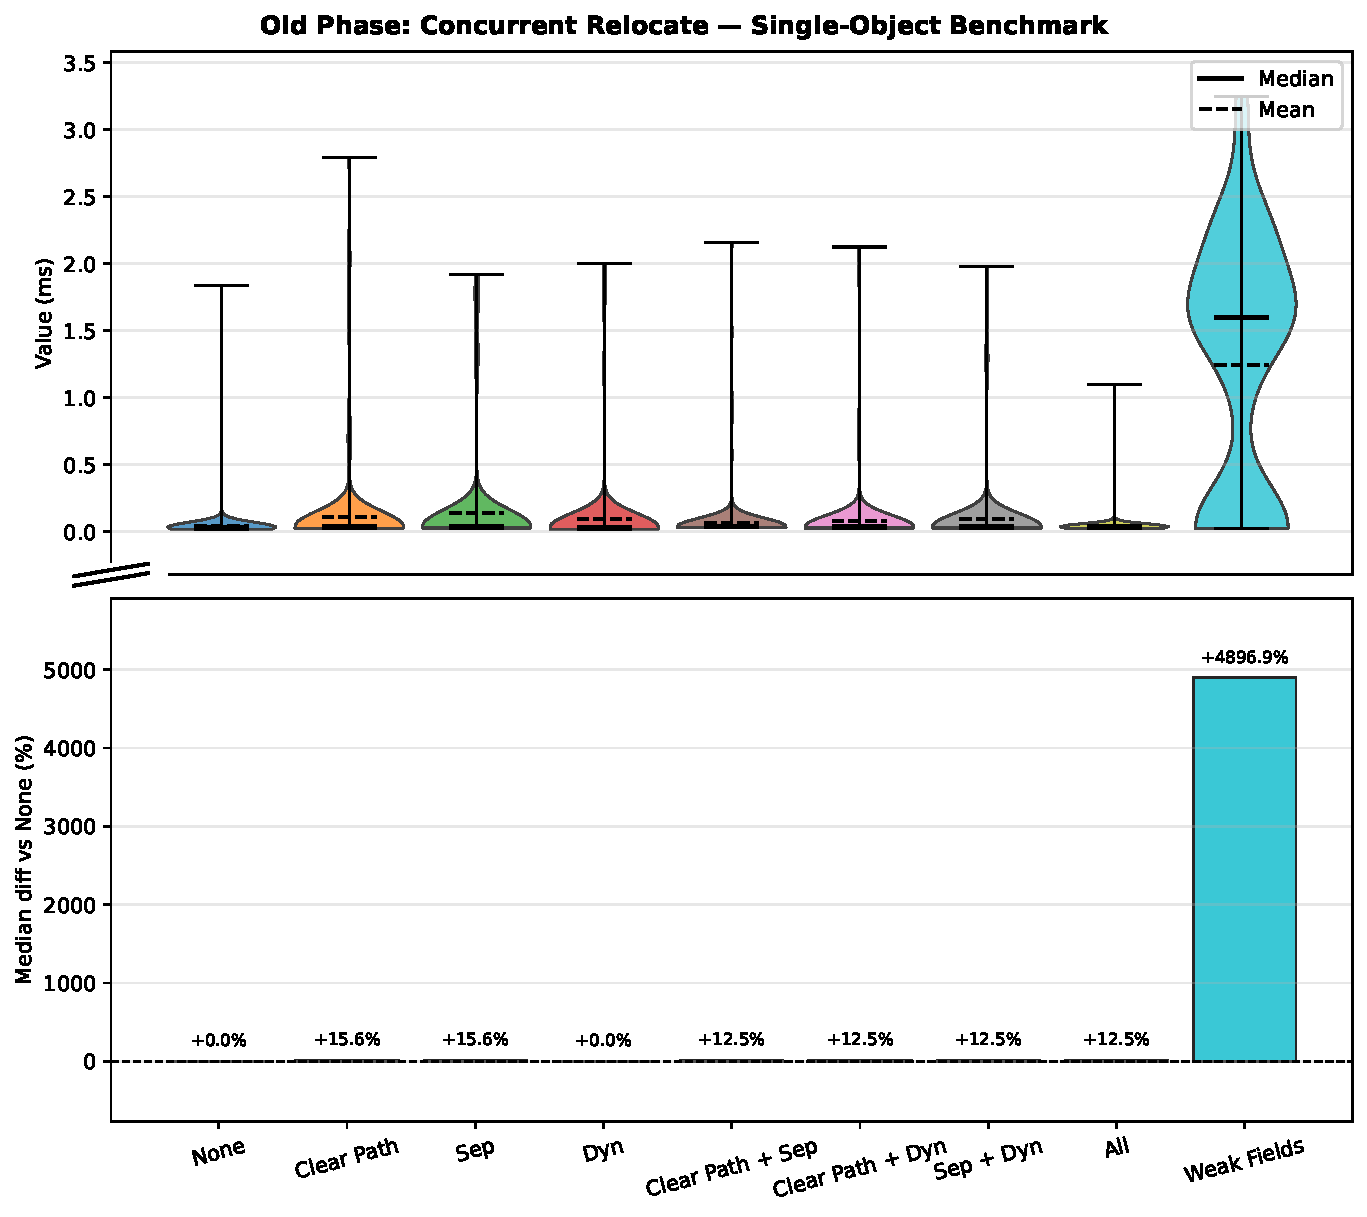
\includegraphics[width=\textwidth]{composite_old_phase_concurrent_relocate_slurm-5118807_combined_gc_single.pdf}
%DIFDELCMD < 	%%%
\DIFdelendFL \DIFaddbeginFL 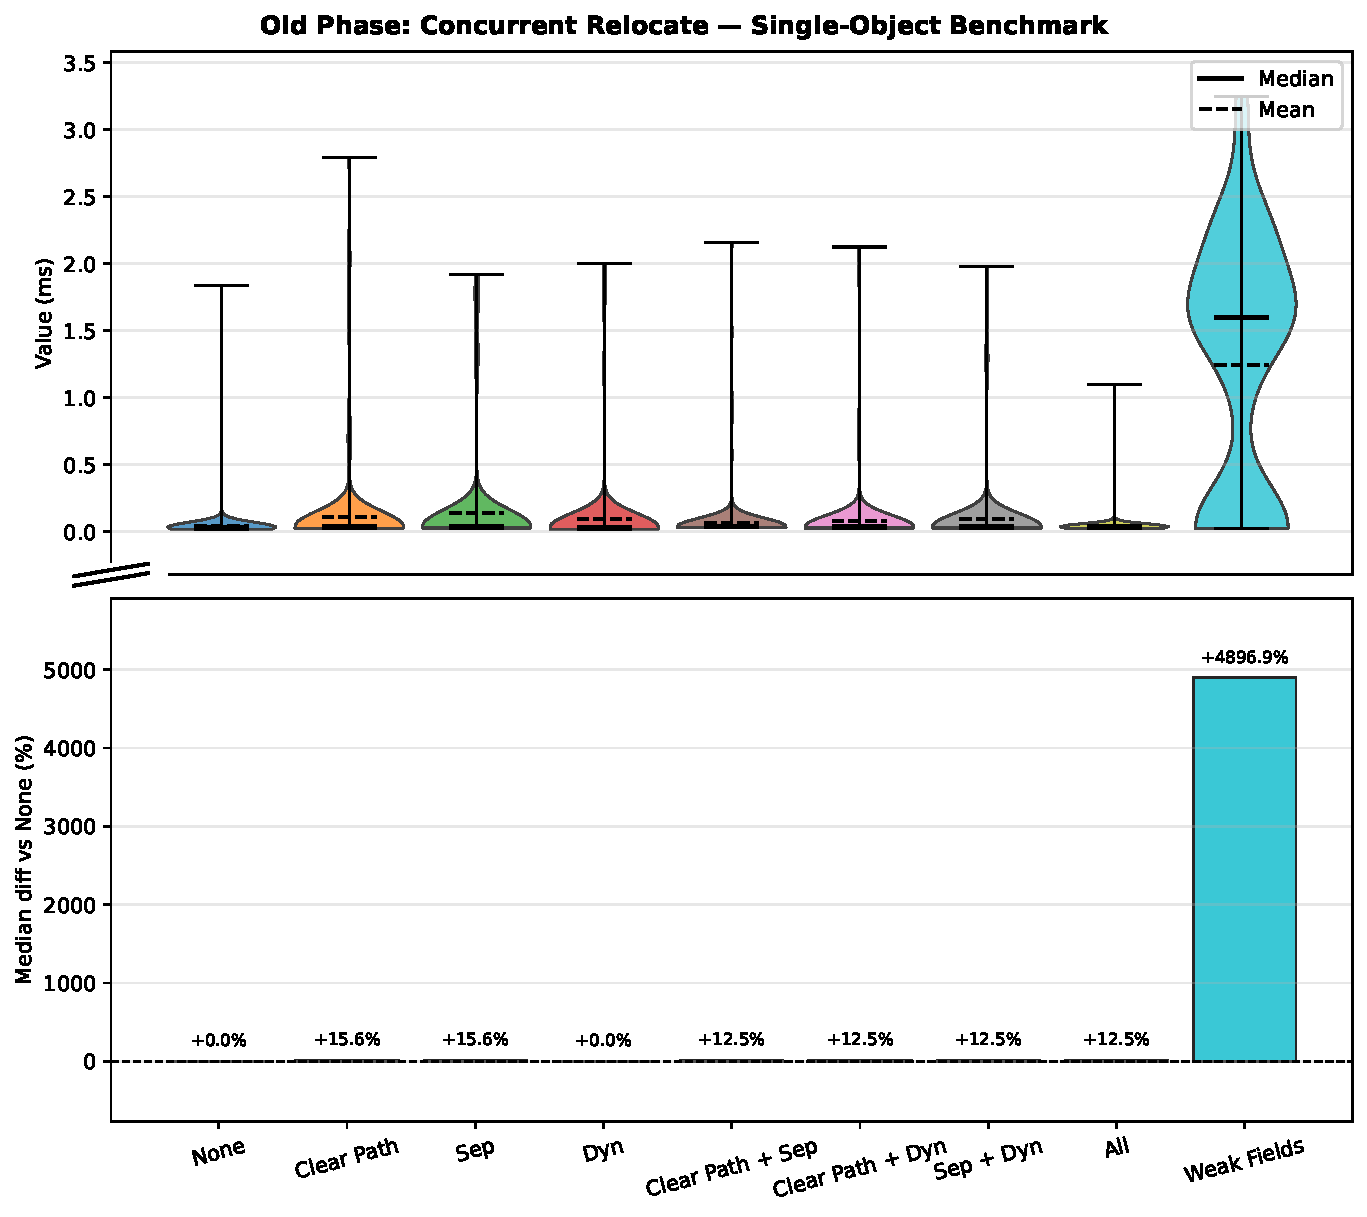
\includegraphics[width=0.8\textwidth]{composite_old_phase_concurrent_relocate_slurm-5118807_combined_gc_single.pdf}
	\DIFaddendFL \caption[Old Phase: Concurrent Relocate timing (single-object)]{Old Phase: Concurrent Relocate timing, \DIFdelbeginFL \DIFdelFL{single-object benchmark }\DIFdelendFL \DIFaddbeginFL \textbf{\DIFaddFL{single-object benchmark}} \DIFaddendFL (per-run maxima). Top: distribution, bottom: median \,\% difference vs baseline.}
	\label{fig:app-gc-single-old-relocate}
\end{figure}

% ---------- Old Phase: Concurrent Relocate – multi ----------
\begin{figure}[t]
	\centering
	\DIFdelbeginFL %DIFDELCMD < 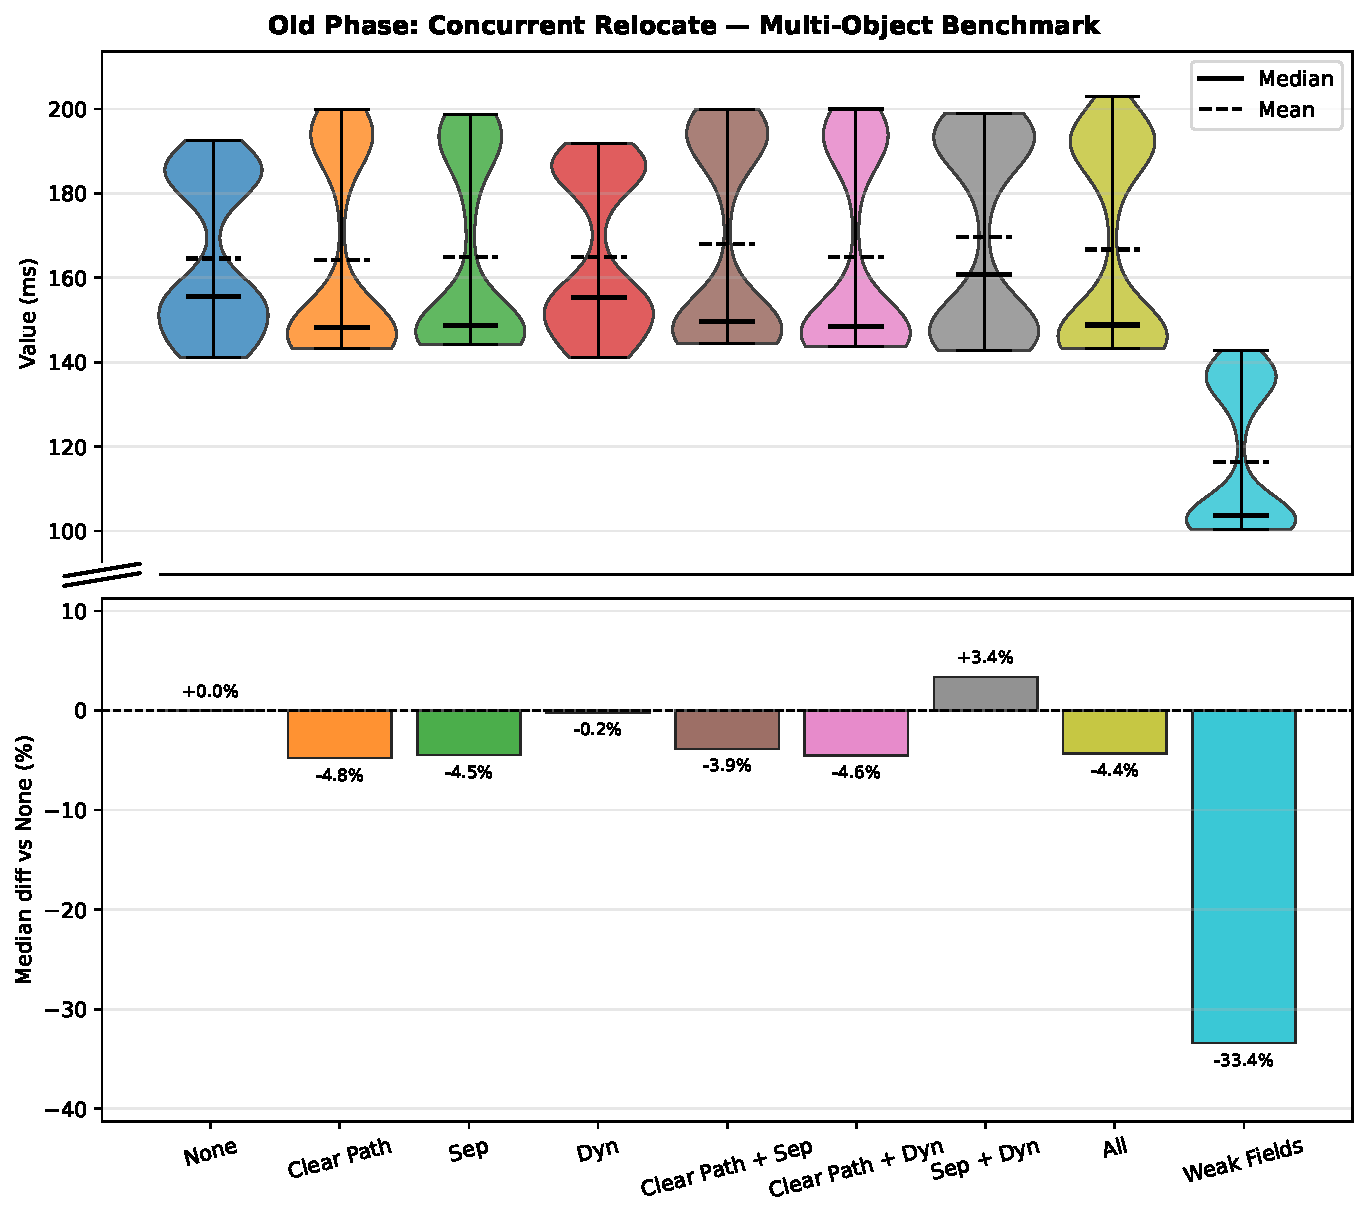
\includegraphics[width=\textwidth]{composite_old_phase_concurrent_relocate_slurm-5118807_combined_gc_multi.pdf}
%DIFDELCMD < 	%%%
\DIFdelendFL \DIFaddbeginFL 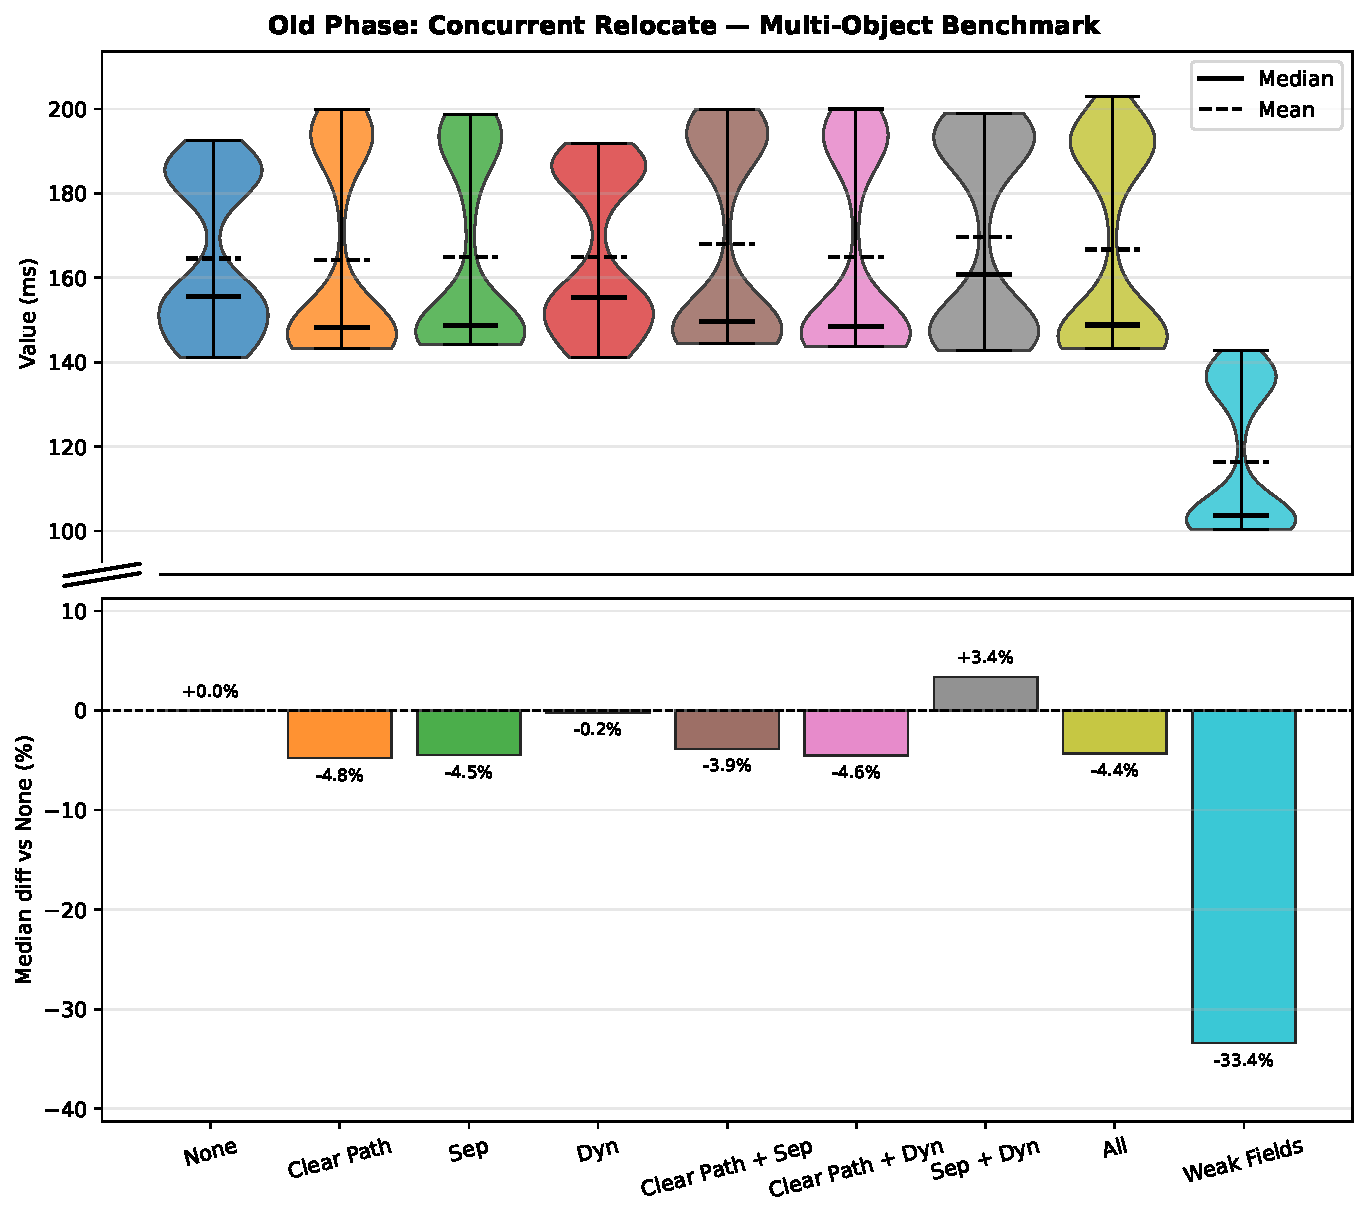
\includegraphics[width=0.8\textwidth]{composite_old_phase_concurrent_relocate_slurm-5118807_combined_gc_multi.pdf}
	\DIFaddendFL \caption[Old Phase: Concurrent Relocate timing (multi-object)]{Old Phase: Concurrent Relocate timing, \DIFdelbeginFL \DIFdelFL{multi-object benchmark }\DIFdelendFL \DIFaddbeginFL \textbf{\DIFaddFL{multi-object benchmark}} \DIFaddendFL (per-run averages). Top: distribution, bottom: median \,\% difference vs baseline.}
	\label{fig:app-gc-multi-old-relocate}
\end{figure}

% ---------- Young Phase: Concurrent Mark – single ----------
\begin{figure}[t]
	\centering
	\DIFdelbeginFL %DIFDELCMD < 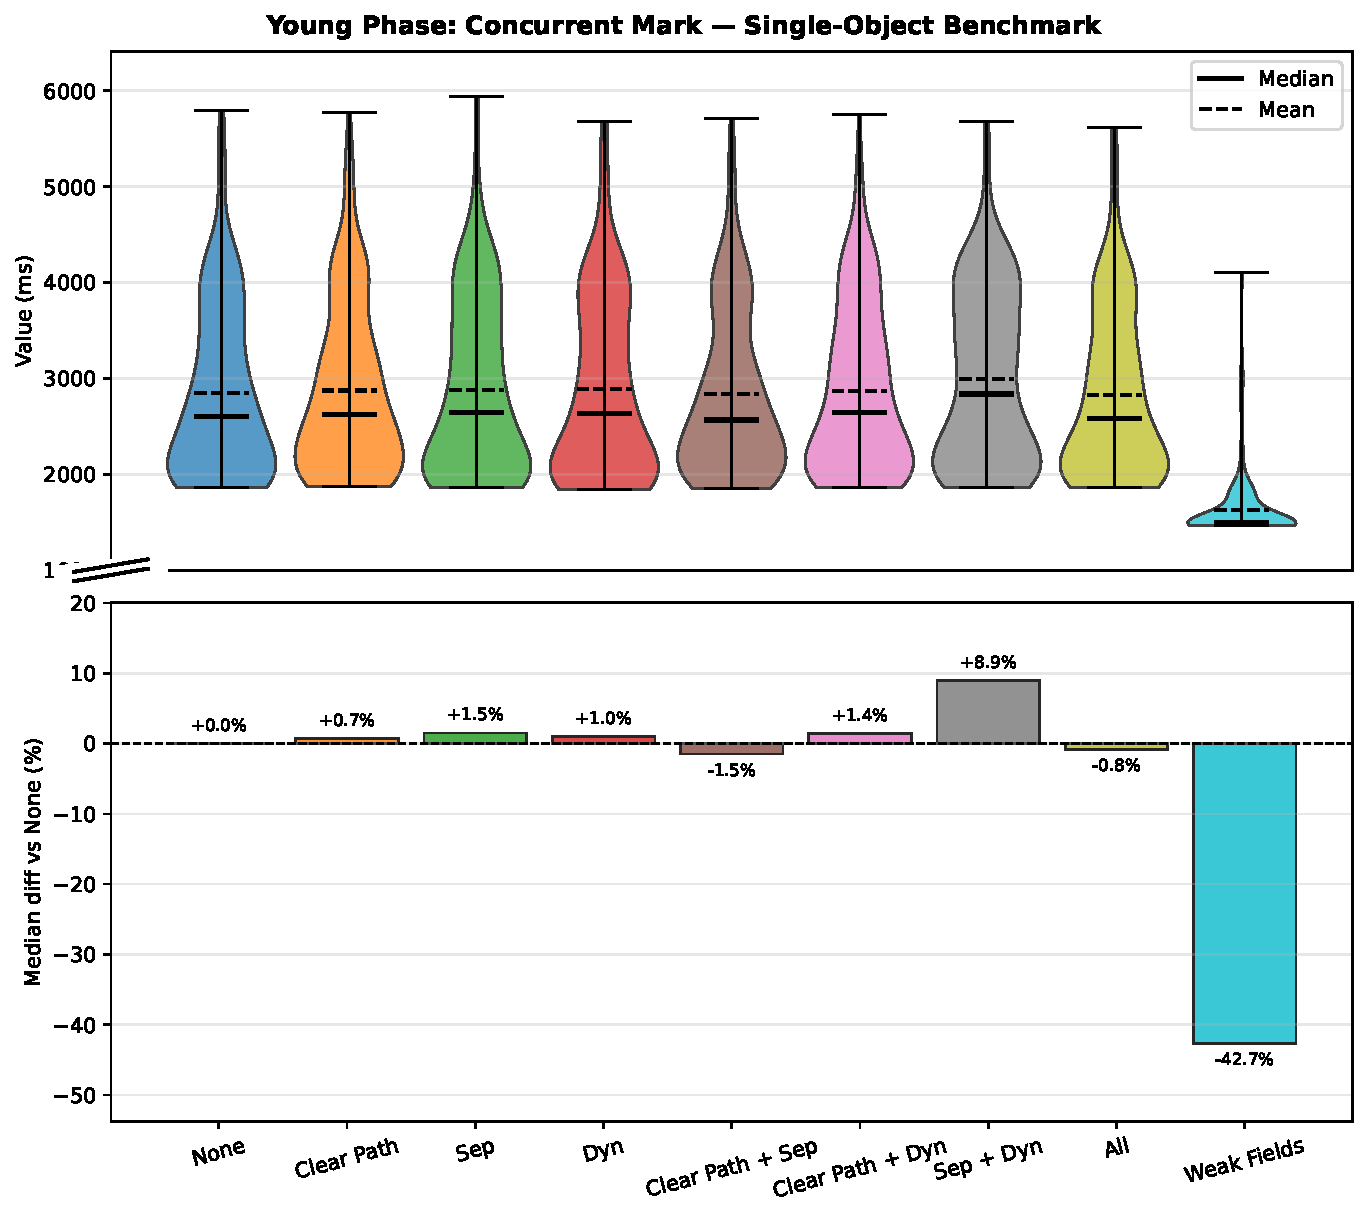
\includegraphics[width=\textwidth]{composite_young_phase_concurrent_mark_slurm-5118807_combined_gc_single.pdf}
%DIFDELCMD < 	%%%
\DIFdelendFL \DIFaddbeginFL 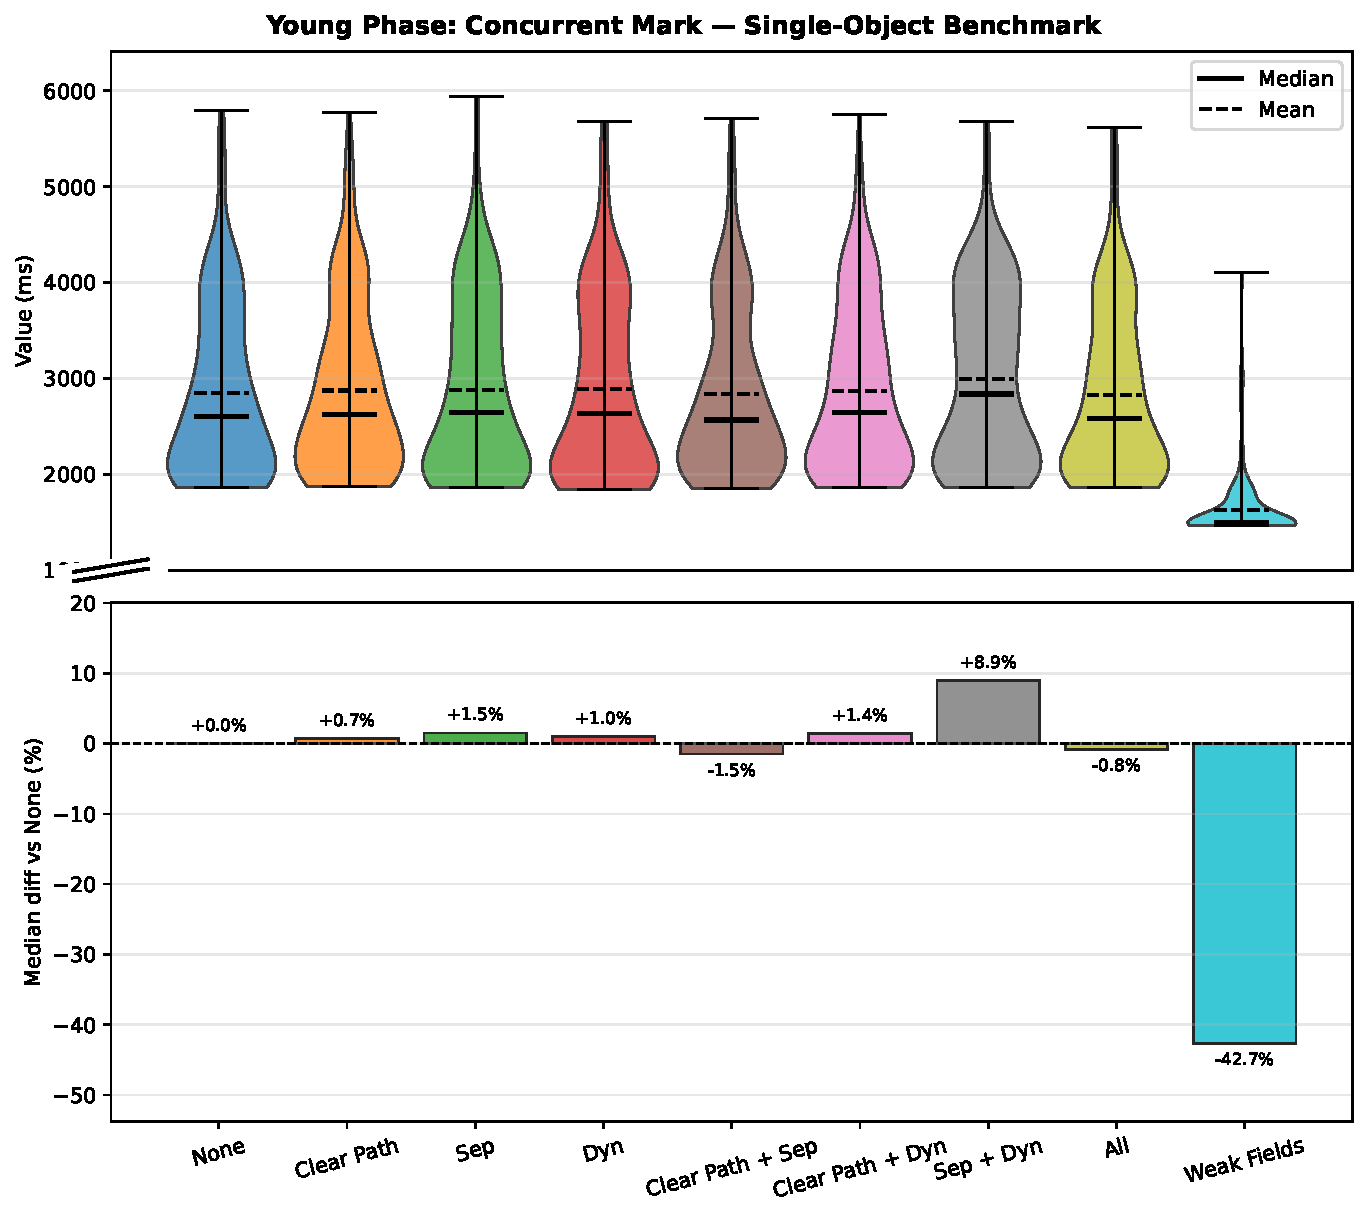
\includegraphics[width=0.8\textwidth]{composite_young_phase_concurrent_mark_slurm-5118807_combined_gc_single.pdf}
	\DIFaddendFL \caption[Young Phase: Concurrent Mark timing (single-object)]{Young Phase: Concurrent Mark timing, \DIFdelbeginFL \DIFdelFL{single-object benchmark }\DIFdelendFL \DIFaddbeginFL \textbf{\DIFaddFL{single-object benchmark}} \DIFaddendFL (per-run maxima). Top: distribution, bottom: median \,\% difference vs baseline.}
	\label{fig:app-gc-single-young-mark}
\end{figure}

% ---------- Young Phase: Concurrent Mark – multi ----------
\begin{figure}[t]
	\centering
	\DIFdelbeginFL %DIFDELCMD < 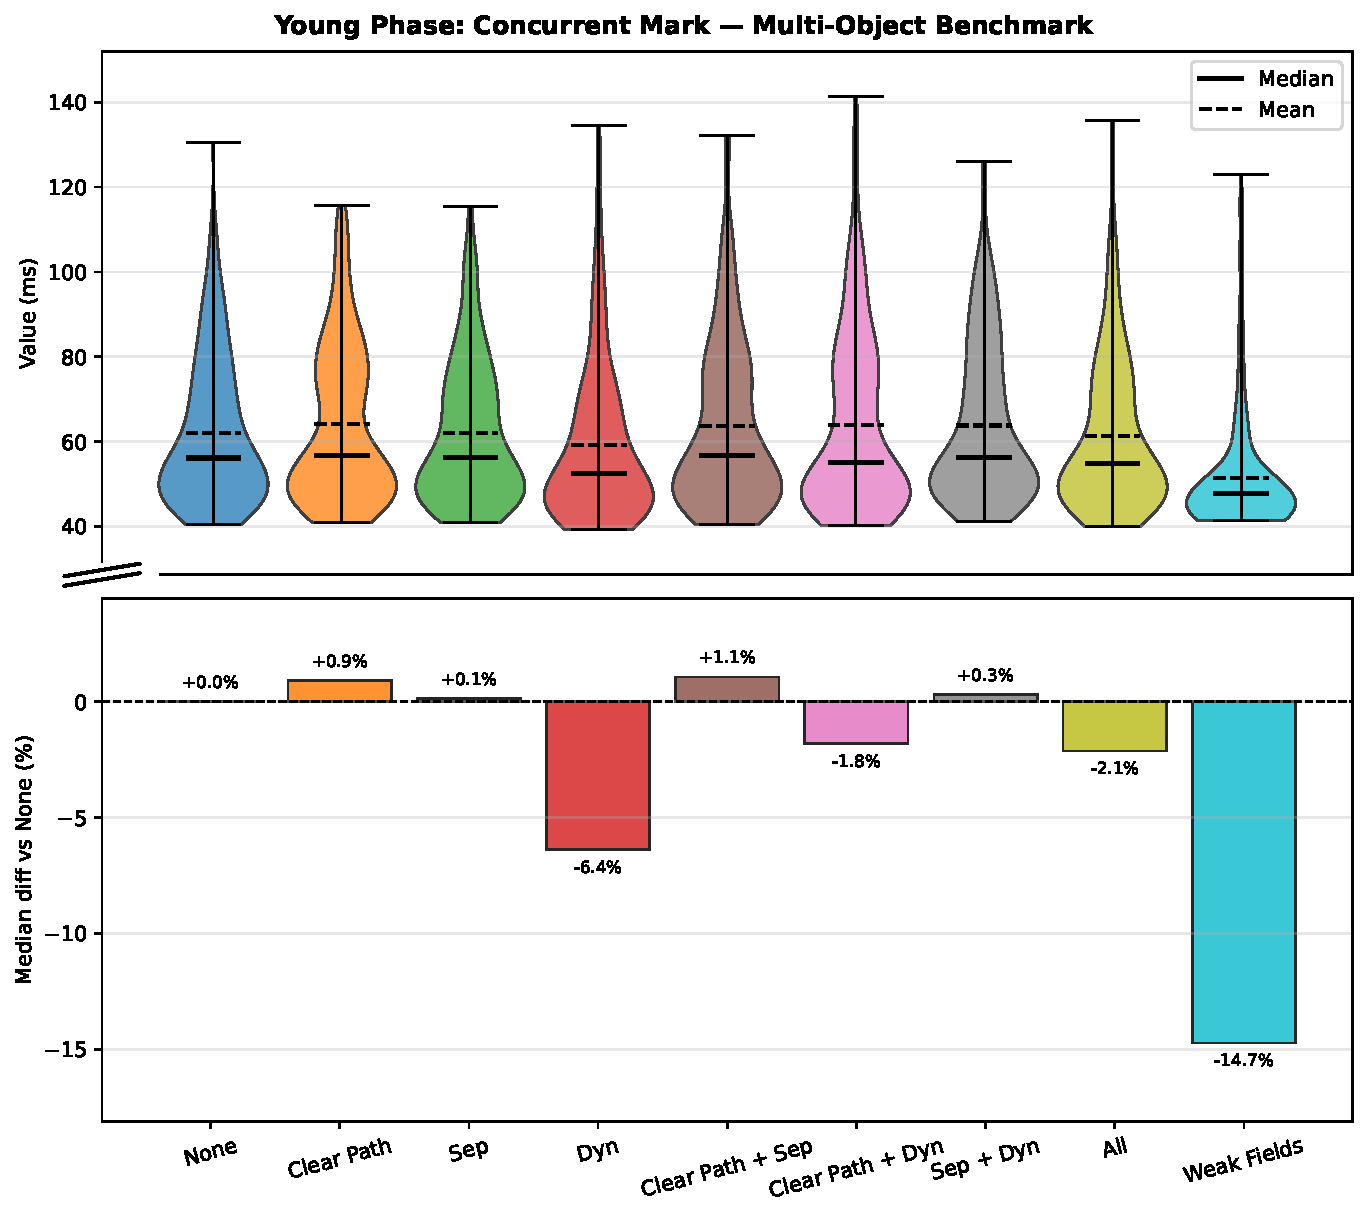
\includegraphics[width=\textwidth]{composite_young_phase_concurrent_mark_slurm-5118807_combined_gc_multi.pdf}
%DIFDELCMD < 	%%%
\DIFdelendFL \DIFaddbeginFL 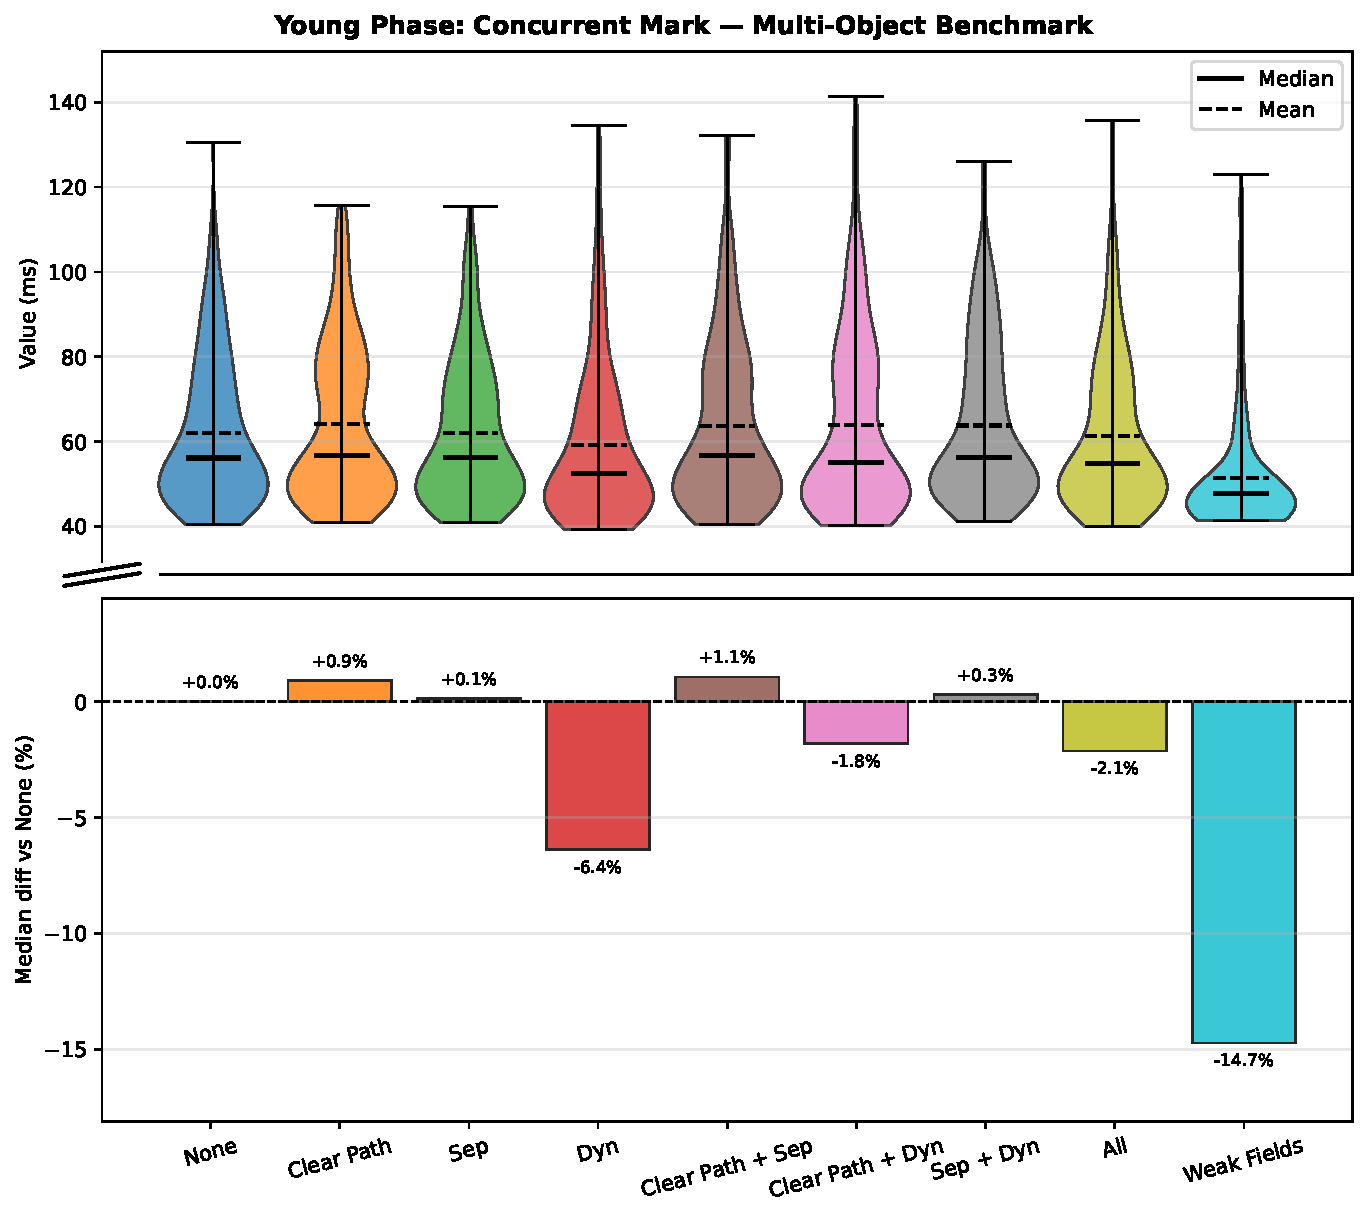
\includegraphics[width=0.8\textwidth]{composite_young_phase_concurrent_mark_slurm-5118807_combined_gc_multi.pdf}
	\DIFaddendFL \caption[Young Phase: Concurrent Mark timing (multi-object)]{Young Phase: Concurrent Mark timing, \DIFdelbeginFL \DIFdelFL{multi-object benchmark }\DIFdelendFL \DIFaddbeginFL \textbf{\DIFaddFL{multi-object benchmark}} \DIFaddendFL (per-run averages). Top: distribution, bottom: median \,\% difference vs baseline.}
	\label{fig:app-gc-multi-young-mark}
\end{figure}

% ---------- Young Phase: Concurrent Relocate – single ----------
\begin{figure}[t]
	\centering
	\DIFdelbeginFL %DIFDELCMD < 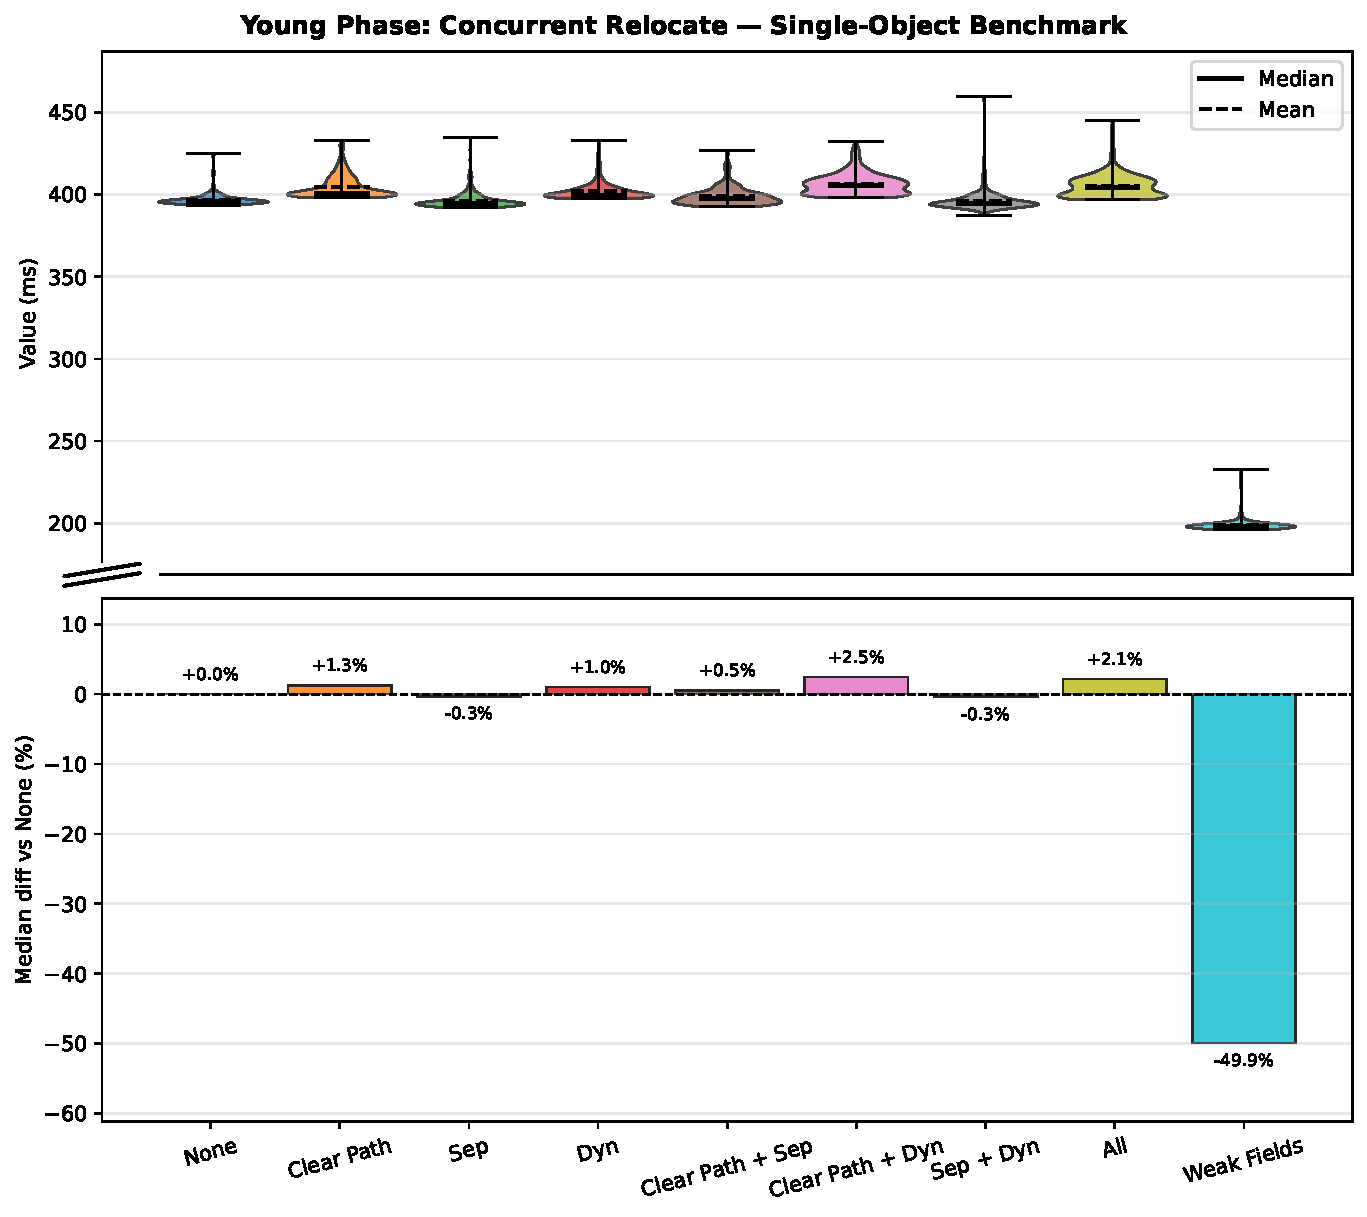
\includegraphics[width=\textwidth]{composite_young_phase_concurrent_relocate_slurm-5118807_combined_gc_single.pdf}
%DIFDELCMD < 	%%%
\DIFdelendFL \DIFaddbeginFL 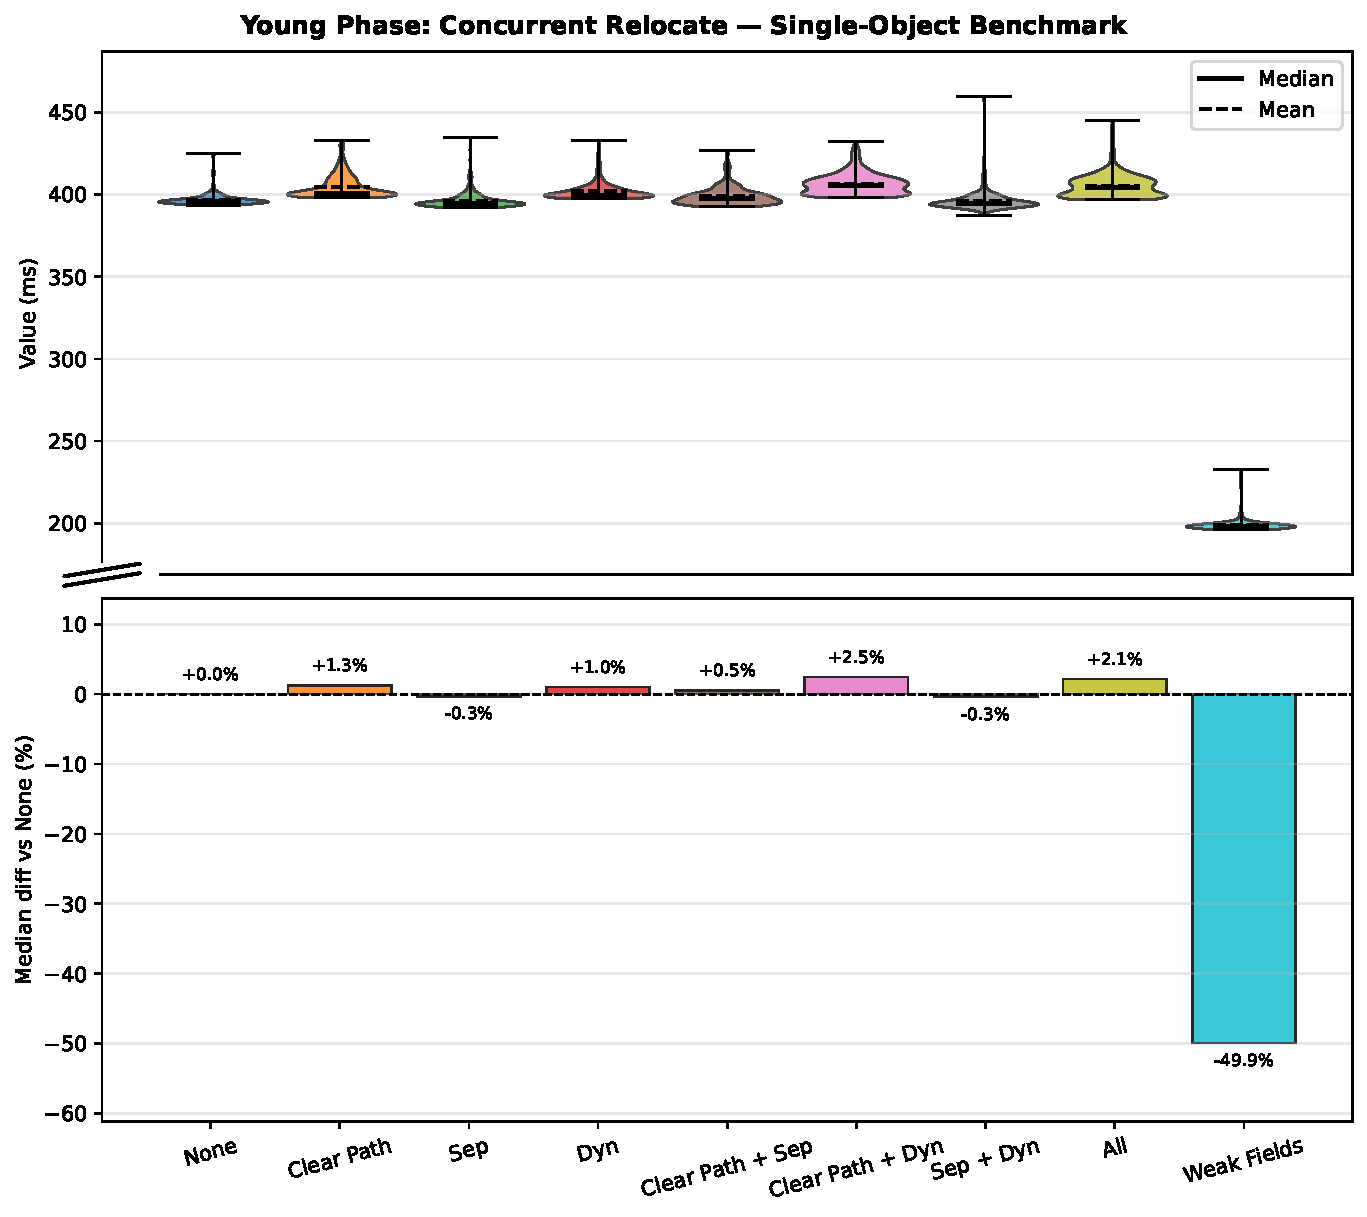
\includegraphics[width=0.8\textwidth]{composite_young_phase_concurrent_relocate_slurm-5118807_combined_gc_single.pdf}
	\DIFaddendFL \caption[Young Phase: Concurrent Relocate timing (single-object)]{Young Phase: Concurrent Relocate timing, \DIFdelbeginFL \DIFdelFL{single-object benchmark }\DIFdelendFL \DIFaddbeginFL \textbf{\DIFaddFL{single-object benchmark}} \DIFaddendFL (per-run maxima). Top: distribution, bottom: median \,\% difference vs baseline.}
	\label{fig:app-gc-single-young-relocate}
\end{figure}

% ---------- Young Phase: Concurrent Relocate – multi ----------
\begin{figure}[t]
	\centering
	\DIFdelbeginFL %DIFDELCMD < 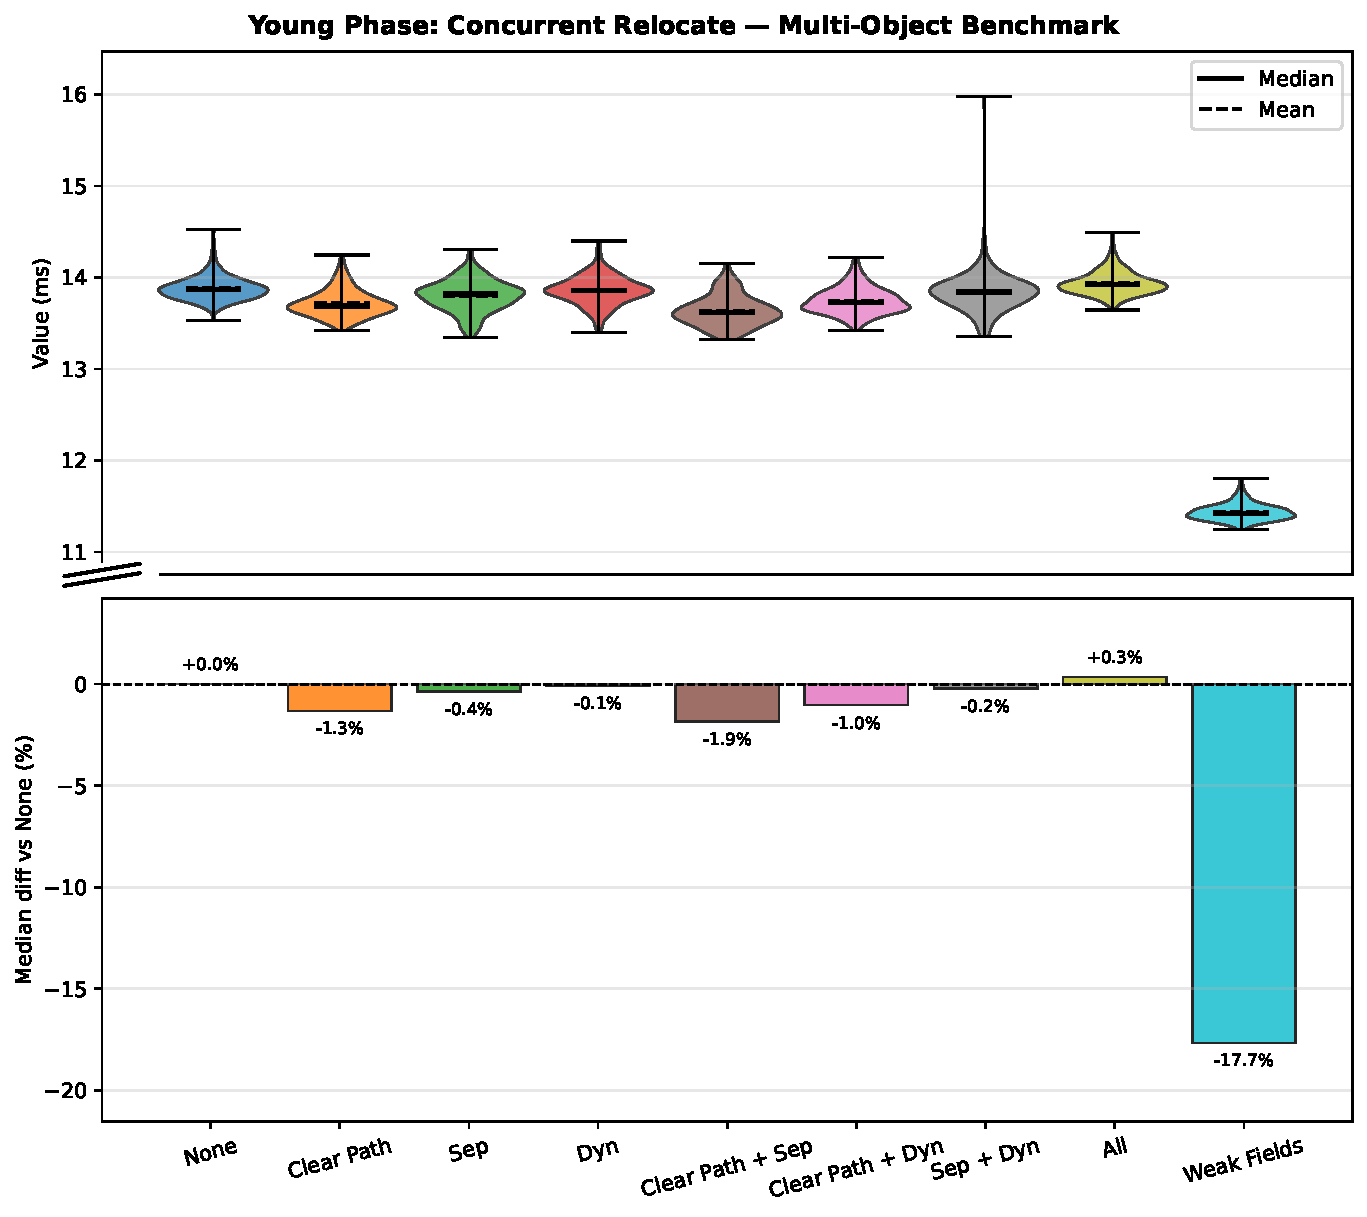
\includegraphics[width=\textwidth]{composite_young_phase_concurrent_relocate_slurm-5118807_combined_gc_multi.pdf}
%DIFDELCMD < 	%%%
\DIFdelendFL \DIFaddbeginFL 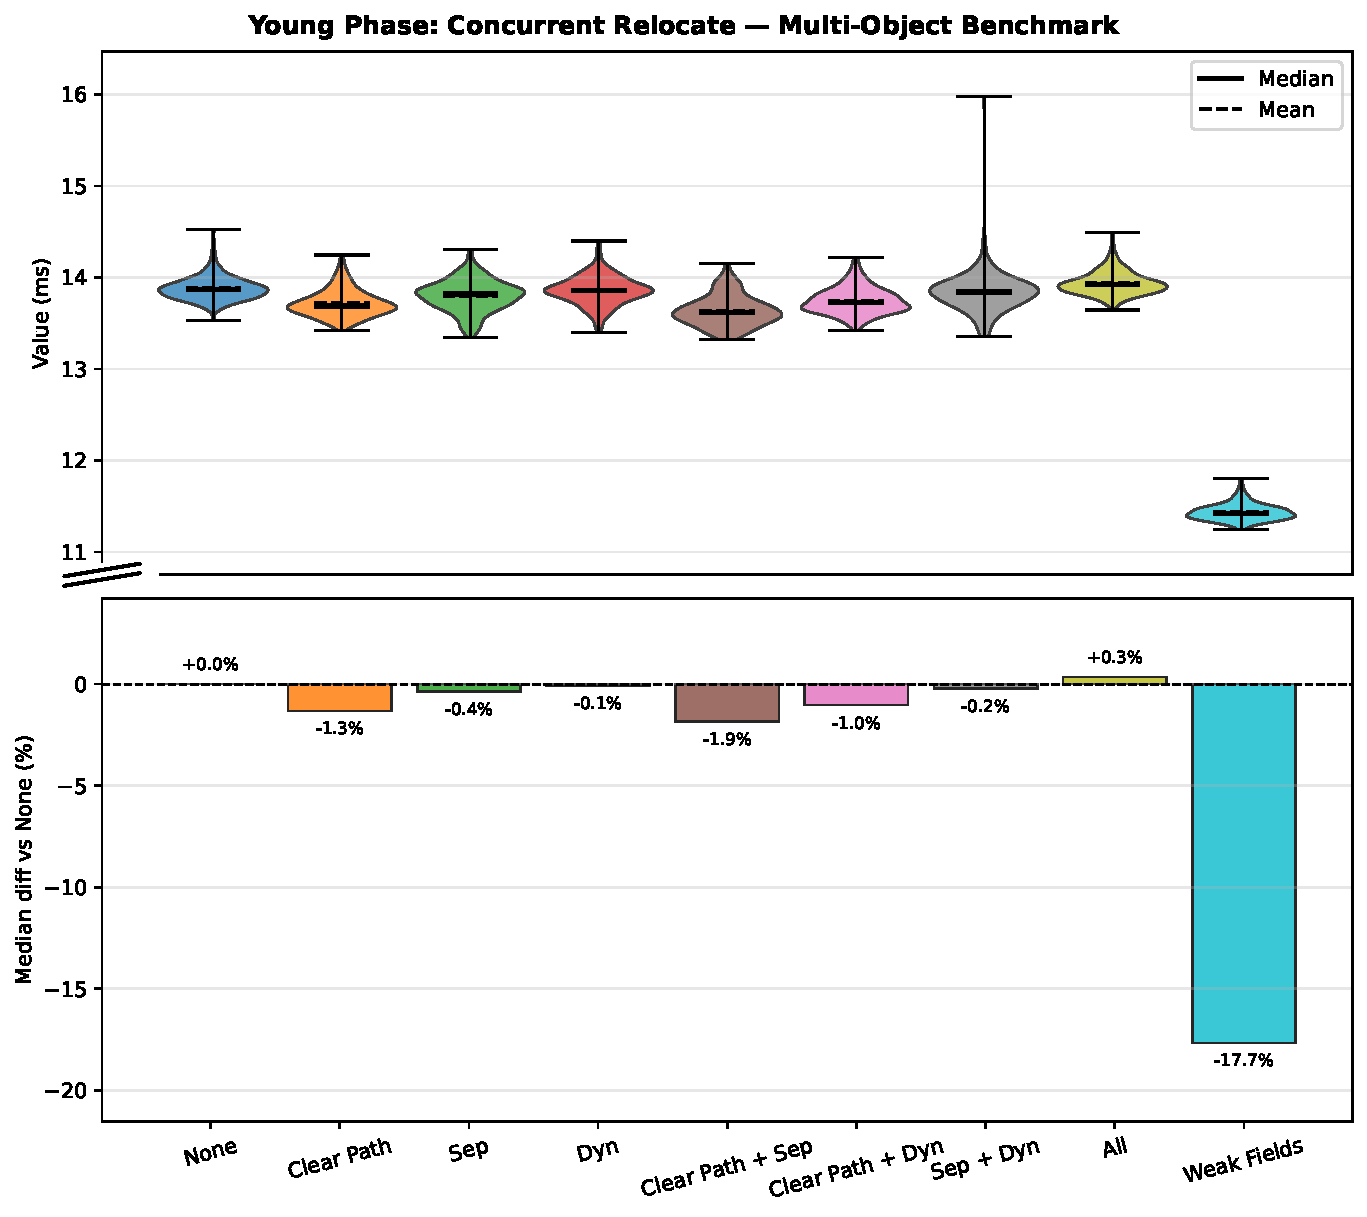
\includegraphics[width=0.8\textwidth]{composite_young_phase_concurrent_relocate_slurm-5118807_combined_gc_multi.pdf}
	\DIFaddendFL \caption[Young Phase: Concurrent Relocate timing (multi-object)]{Young Phase: Concurrent Relocate timing, \DIFdelbeginFL \DIFdelFL{multi-object benchmark }\DIFdelendFL \DIFaddbeginFL \textbf{\DIFaddFL{multi-object benchmark}} \DIFaddendFL (per-run averages). Top: distribution, bottom: median \,\% difference vs baseline.}
	\label{fig:app-gc-multi-young-relocate}
\end{figure}

% ---------- Memory max distributions – single ----------
\begin{figure}[t]
	\centering
	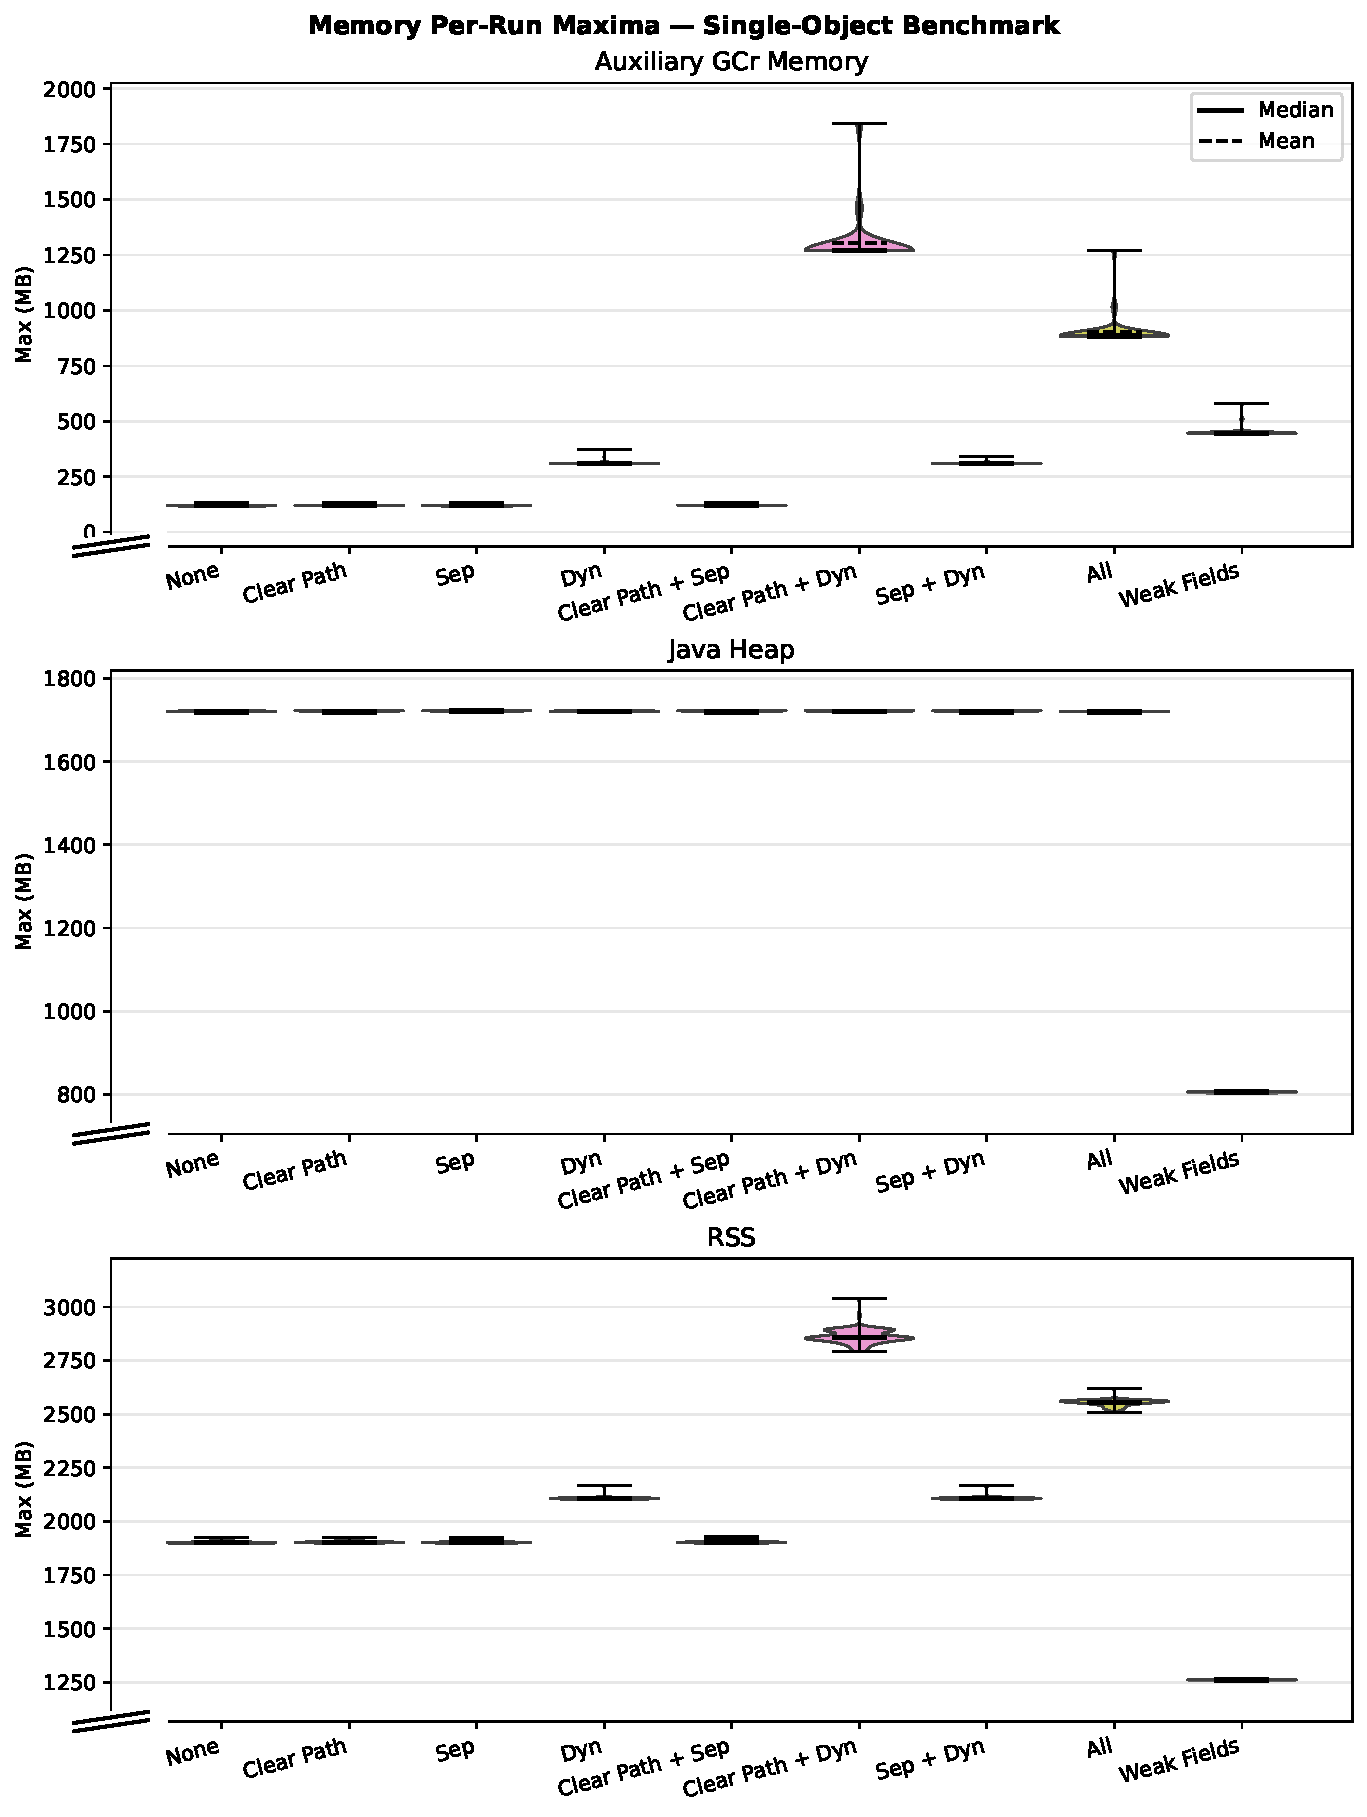
\includegraphics[width=\textwidth]{memory_max_slurm-5118807_combined_gc_single.pdf}
	\caption[Memory per-run maximum distributions (single-object)]{Distribution of per-run maximum memory across variants, \DIFdelbeginFL \DIFdelFL{single-object benchmark}\DIFdelendFL \DIFaddbeginFL \textbf{\DIFaddFL{single-object benchmark}}\DIFaddendFL . Top to bottom: auxiliary \DIFdelbeginFL %DIFDELCMD < \ac{GC} %%%
\DIFdelendFL \DIFaddbeginFL \ac{GCr} \DIFaddendFL memory, Java heap, total process \ac{RSS}.}
	\label{fig:app-mem-single-max}
\end{figure}

% ---------- Memory max distributions – multi ----------
\begin{figure}[t]
	\centering
	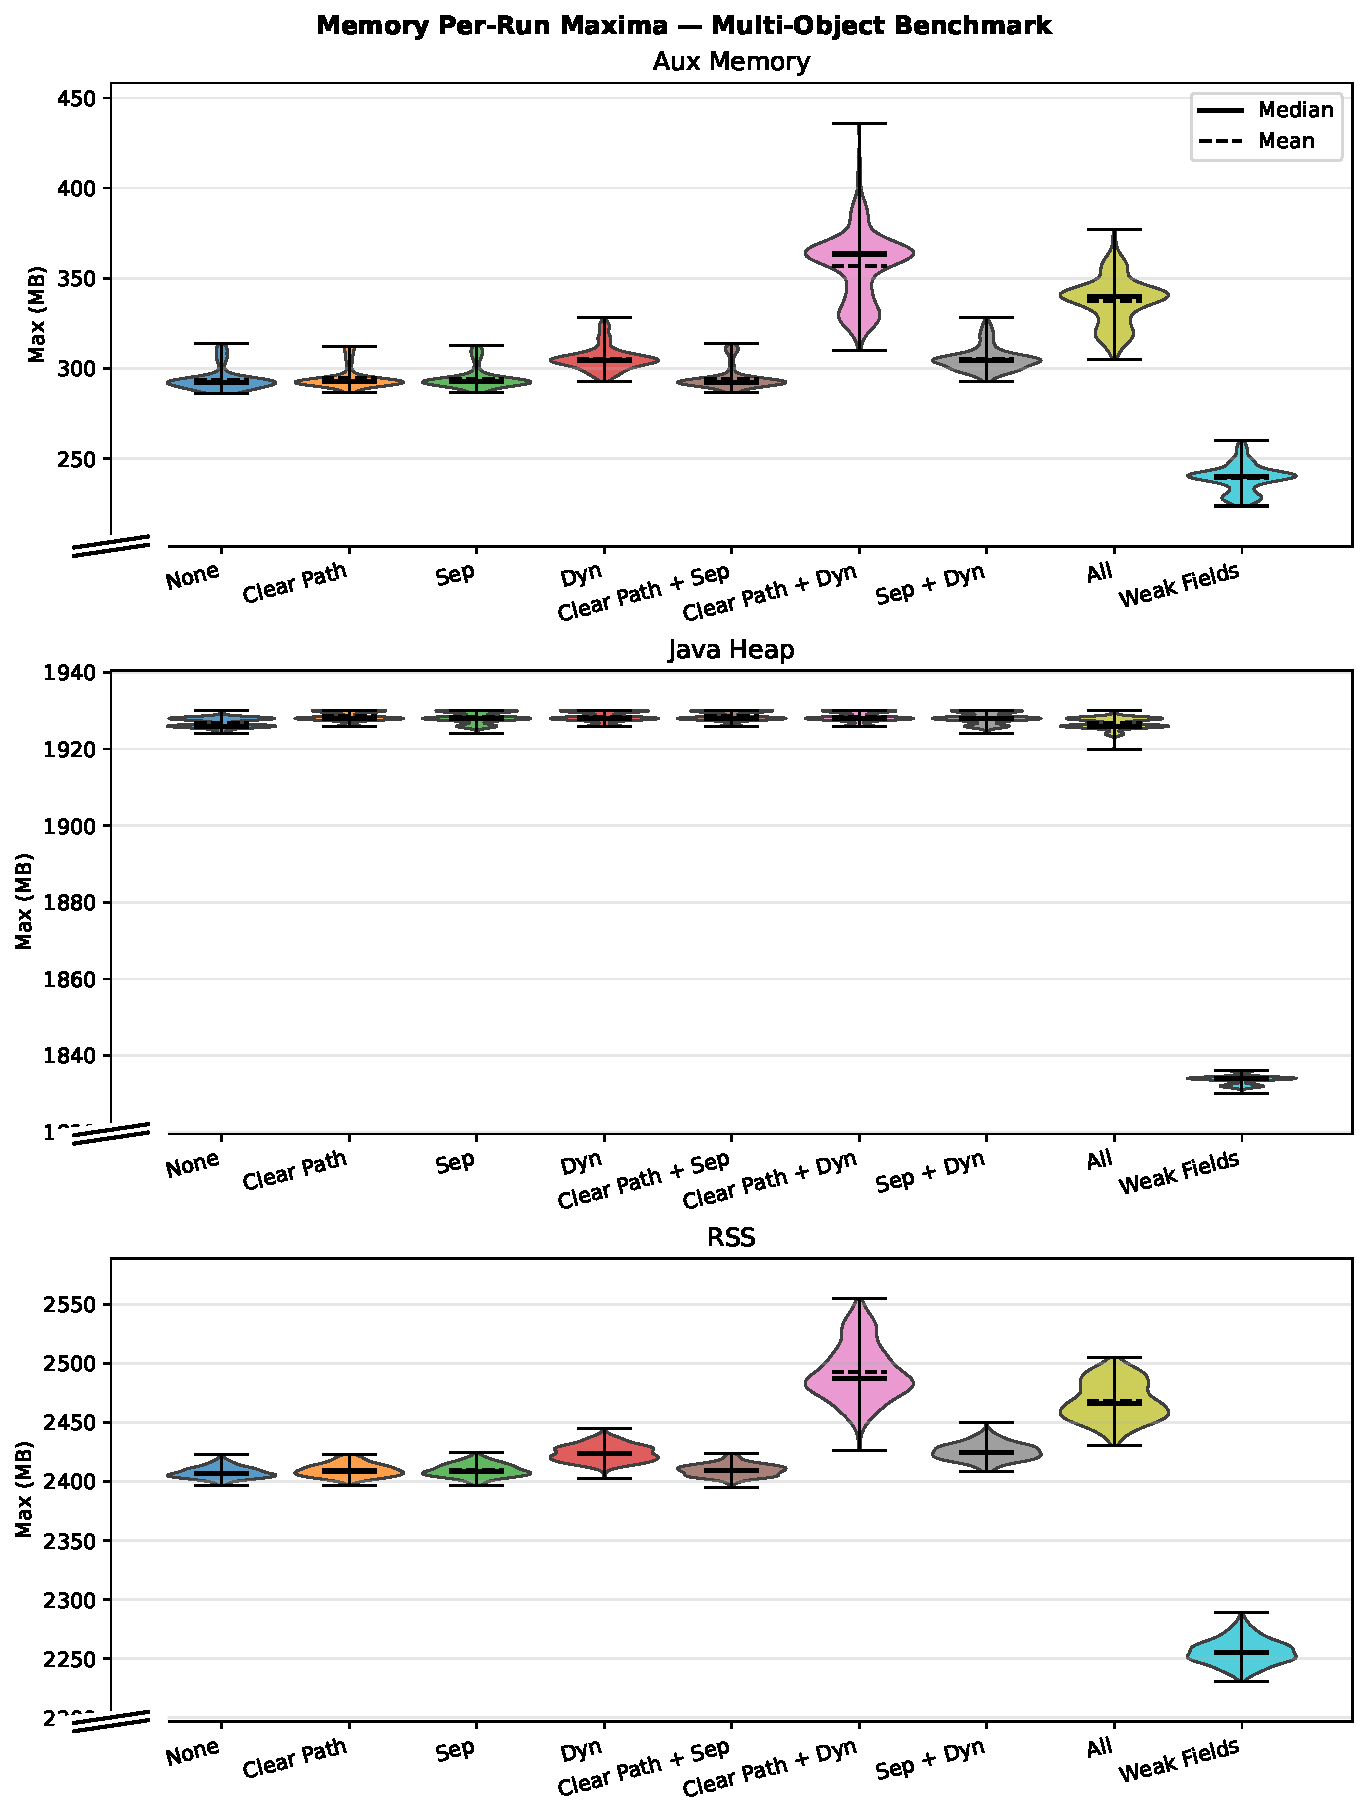
\includegraphics[width=\textwidth]{memory_max_slurm-5118807_combined_gc_multi.pdf}
	\caption[Memory per-run maximum distributions (multi-object)]{Distribution of per-run maximum memory across variants, \DIFdelbeginFL \DIFdelFL{multi-object benchmark}\DIFdelendFL \DIFaddbeginFL \textbf{\DIFaddFL{multi-object benchmark}}\DIFaddendFL . Top to bottom: auxiliary \DIFdelbeginFL %DIFDELCMD < \ac{GC} %%%
\DIFdelendFL \DIFaddbeginFL \ac{GCr} \DIFaddendFL memory, Java heap, total process \ac{RSS}.}
	\label{fig:app-mem-multi-max}
\end{figure}
\DIFaddbegin 

%DIF >  ---------- Ratio of non-strong processing time to total major collection time – single ----------
\begin{figure}[t]
	\centering
	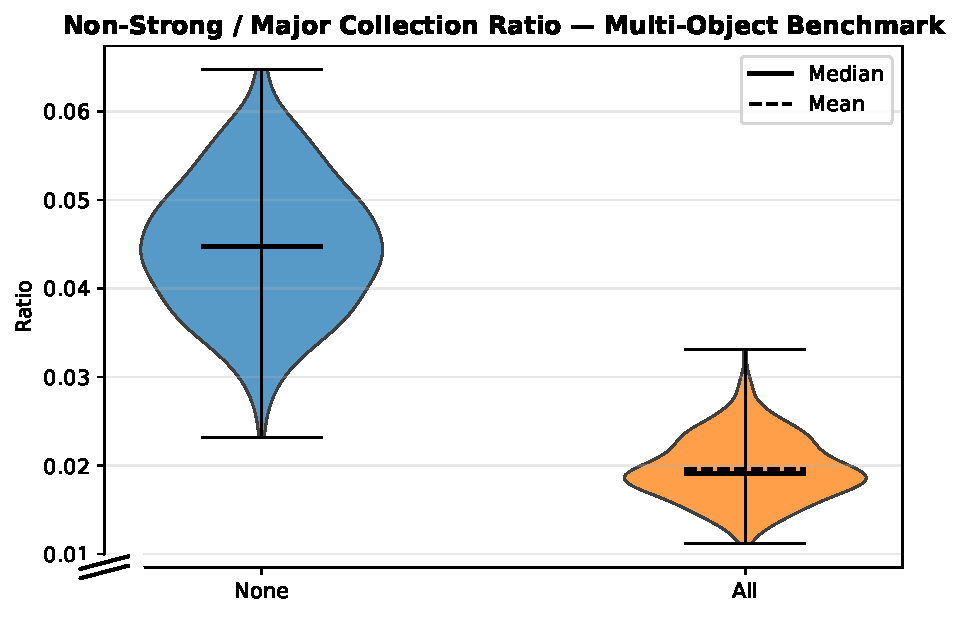
\includegraphics[width=\textwidth]{ratio_violin_slurm-5118807_combined_gc_multi.pdf}
	\caption[Ratio of non-strong processing time to total major collection time]{\DIFaddFL{Ratio of non-strong processing time to total major collection time, }\textbf{\DIFaddFL{multi-object benchmark}} \DIFaddFL{(per-run averages). Distribution across variants.}}
	\label{fig:app-ratio-nonstrong-multi}
\end{figure}

%DIF >  ---------- Ratio of non-strong processing time to total major collection time – multi ----------
\begin{figure}[t]
	\centering
	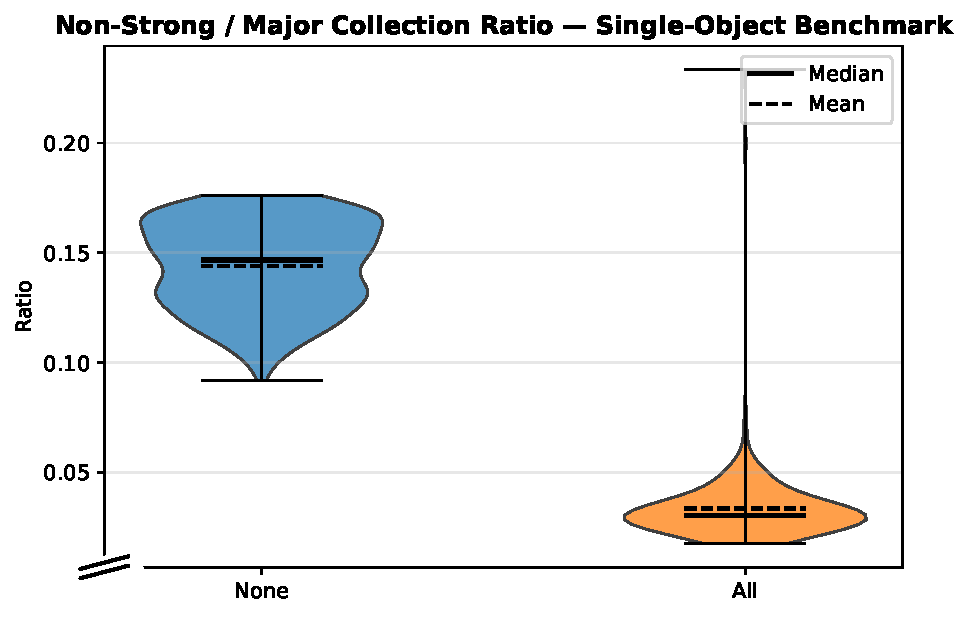
\includegraphics[width=\textwidth]{ratio_violin_slurm-5118807_combined_gc_single.pdf}
	\caption[Ratio of non-strong processing time to total major collection time]{\DIFaddFL{Ratio of non-strong processing time to total major collection time, }\textbf{\DIFaddFL{single-object benchmark}} \DIFaddFL{(per-run maxima). Distribution across variants.}}
	\label{fig:app-ratio-nonstrong-single}
\end{figure}

\DIFaddend \chapter{Source Code}
\label{app:source}

This appendix provides the key source code for the implemented optimisations. The code for the three core optimisations is from the combined (\texttt{all}) configuration variant, which includes all three optimisations. The code for the weak-field mechanism is from the \texttt{weak\_fields} configuration variant. Complete sources for all variants are available in the \texttt{patches/} directory of the project repository.

\lstset{basicstyle=\ttfamily\footnotesize,columns=flexible}

\section{Dynamic-array Data Structure}
\label{app:source-dyn}
\refstepcounter{listing}
\addcontentsline{lol}{listing}{\protect\numberline{\thelisting}\texttt{zWeakRefArray.hpp}: Dynamic-array data structure}

\DIFaddbegin \DIFadd{The }\texttt{\DIFadd{ZWeakRefArray}} \DIFadd{template is the central data structure for the dynamic-array optimisation. It stores discovered weak references contiguously on the C heap, enabling sequential traversal without pointer chasing. Each entry in the extended variant (}\texttt{\DIFadd{ZWeakRefDataExt}}\DIFadd{) pre-loads the referent field address and value during discovery so that the clear path can operate without additional heap loads. Note in particular the }\texttt{\DIFadd{clear\_and\_reserve}} \DIFadd{method, which retains capacity between }\ac{GC} \DIFadd{cycles to avoid repeated reallocation when the reference population is stable.
}

\DIFaddend \noindent\textbf{File:} \texttt{zWeakRefArray.hpp}

\begin{lstlisting}[
	nolol,
	language=C++
]
/*
 * Copyright (c) 2025, Oracle and/or its affiliates. All rights reserved.
 * DO NOT ALTER OR REMOVE COPYRIGHT NOTICES OR THIS FILE HEADER.
 *
 * This code is free software; you can redistribute it and/or modify it
 * under the terms of the GNU General Public License version 2 only, as
 * published by the Free Software Foundation.
 *
 * This code is distributed in the hope that it will be useful, but WITHOUT
 * ANY WARRANTY; without even the implied warranty of MERCHANTABILITY or
 * FITNESS FOR A PARTICULAR PURPOSE.  See the GNU General Public License
 * version 2 for more details (a copy is included in the LICENSE file that
 * accompanied this code).
 *
 * You should have received a copy of the GNU General Public License version
 * 2 along with this work; if not, write to the Free Software Foundation,
 * Inc., 51 Franklin St, Fifth Floor, Boston, MA 02110-1301 USA.
 *
 * Please contact Oracle, 500 Oracle Parkway, Redwood Shores, CA 94065 USA
 * or visit www.oracle.com if you need additional information or have any
 * questions.
 */

#ifndef SHARE_GC_Z_ZWEAKREFARRAY_HPP
#define SHARE_GC_Z_ZWEAKREFARRAY_HPP

#include "gc/z/zAddress.hpp"
#include "memory/allocation.hpp"
#include "utilities/debug.hpp"
#include "utilities/powerOfTwo.hpp"
#include "utilities/globalDefinitions.hpp"
#include <string.h>

struct ZWeakRefData {
  zpointer* referent_field_addr;
  zaddress* discovered_field_addr;
  zaddress referent_addr;
  zpointer referent_field_value;
};


class ZWeakRefArray : public AnyObj {
private:
  ZWeakRefData* _data;
  const size_t _ZWeakRefData_size = sizeof(ZWeakRefData);
  size_t _length;
  size_t _capacity;

  void expand_to(size_t new_capacity) {
    assert(new_capacity > _capacity, "expected growth but %ld <= %ld", new_capacity, _capacity);
    
    ZWeakRefData* new_data = (ZWeakRefData*)AllocateHeap(new_capacity * _ZWeakRefData_size, mtGC);
    
    if (_length > 0) {
      // Use memcpy for trivially copyable types - much faster than element-by-element copy
      memcpy(new_data, _data, _length * _ZWeakRefData_size);
    }
    
    if (_data != nullptr) {
      FreeHeap(_data);
    }
    
    _data = new_data;
    _capacity = new_capacity;
  }

  void grow(size_t min_capacity) {
    size_t new_capacity = MAX2((size_t) 8, next_power_of_2(min_capacity - 1));
    expand_to(new_capacity);
  } 

public:
  ZWeakRefArray() : _data(nullptr), _length(0), _capacity(0) {}

  ~ZWeakRefArray() {
    if (_data != nullptr) {
      FreeHeap(_data);
      _data = nullptr;
    }
  }

  void append(const ZWeakRefData& entry) {
    if (_length >= _capacity) {
      grow(_length + 1);
    }
    _data[_length] = entry;
    _length++;
  }

  // Get entry at index
  const ZWeakRefData& at(size_t index) const {
    assert(index < _length, "index out of bounds: %ld (length: %ld)", index, _length);
    return _data[index];
  }

  // Current length
  size_t length() const {
    return _length;
  }

  // Whether the array is empty
  bool is_empty() const {
    return _length == 0;
  }

  // Current capacity
  size_t capacity() const {
    return _capacity;
  }

  void clear_and_reserve(size_t new_capacity) {
    if (new_capacity == 0) {
      // Special case for clearing to empty - free memory and reset
       if (_data != nullptr) {
         FreeHeap(_data);
         _data = nullptr;
       }
       _length = 0;
       _capacity = 0;
       return;
    }
    _length = 0;
    if (_data != nullptr) {
      FreeHeap(_data);
    }
    _capacity = MAX2((size_t) 8, next_power_of_2(new_capacity - 1));
    _data = (ZWeakRefData*)AllocateHeap(_capacity * _ZWeakRefData_size, mtGC);
  }

  // Clear without deallocating
  void clear() {
    _length = 0;
  }

  // Reserve capacity without clearing
  void reserve(size_t new_capacity) {
    if (new_capacity > _capacity) {
      grow(new_capacity);
    }
  }
};

#endif // SHARE_GC_Z_ZWEAKREFARRAY_HPP
\end{lstlisting}


\section{Reference Processor}
\label{app:source-refproc}

\subsection{Interface}
\label{app:source-refproc-iface}
\refstepcounter{listing}
\addcontentsline{lol}{listing}{\protect\numberline{\thelisting}\texttt{zReferenceProcessor.hpp}: Reference processor interface (\texttt{all} variant)}

\DIFaddbegin \DIFadd{The header file shows the per-worker state added by the }\texttt{\DIFadd{all}} \DIFadd{variant: a }\texttt{\DIFadd{ZWeakRefArray}} \DIFadd{for queue-less discovered references (bypassing the pending list), a separate }\texttt{\DIFadd{ZWeakRefArray}} \DIFadd{used by the standard pipeline, and a counter for cleared weak references without a queue. The key type change to notice is }\texttt{\DIFadd{ZWeakRefDataExt}} \DIFadd{in the queue-less path -- this is the extended entry type that pre-loads the referent for the barrier-free clear path.
}

\DIFaddend \noindent\textbf{File:} \texttt{zReferenceProcessor.hpp}

\begin{lstlisting}[
	nolol,
	language=C++
]
/*
 * Copyright (c) 2015, 2024, Oracle and/or its affiliates. All rights reserved.
 * DO NOT ALTER OR REMOVE COPYRIGHT NOTICES OR THIS FILE HEADER.
 *
 * This code is free software; you can redistribute it and/or modify it
 * under the terms of the GNU General Public License version 2 only, as
 * published by the Free Software Foundation.
 *
 * This code is distributed in the hope that it will be useful, but WITHOUT
 * ANY WARRANTY; without even the implied warranty of MERCHANTABILITY or
 * FITNESS FOR A PARTICULAR PURPOSE.  See the GNU General Public License
 * version 2 for more details (a copy is included in the LICENSE file that
 * accompanied this code).
 *
 * You should have received a copy of the GNU General Public License version
 * 2 along with this work; if not, write to the Free Software Foundation,
 * Inc., 51 Franklin St, Fifth Floor, Boston, MA 02110-1301 USA.
 *
 * Please contact Oracle, 500 Oracle Parkway, Redwood Shores, CA 94065 USA
 * or visit www.oracle.com if you need additional information or have any
 * questions.
 */

#ifndef SHARE_GC_Z_ZREFERENCEPROCESSOR_HPP
#define SHARE_GC_Z_ZREFERENCEPROCESSOR_HPP

#include "gc/shared/referenceDiscoverer.hpp"
#include "gc/z/zAddress.hpp"
#include "gc/z/zWeakRefArray.hpp"
#include "gc/z/zValue.hpp"

class ConcurrentGCTimer;
class ReferencePolicy;
class ZWorkers;

class ZReferenceProcessor : public ReferenceDiscoverer {
  friend class ZReferenceProcessorTask;

private:
  static const size_t ReferenceTypeCount = REF_PHANTOM + 1;
  typedef size_t Counters[ReferenceTypeCount];

  ZWorkers* const           _workers;
  ReferencePolicy*          _soft_reference_policy;
  bool                      _uses_clear_all_soft_reference_policy;
  ZPerWorker<Counters>      _encountered_count;
  ZPerWorker<Counters>      _discovered_count;
  ZPerWorker<Counters>      _enqueued_count;
  ZPerWorker<size_t>        _encountered_weak_refs_without_queue_count;
  ZPerWorker<size_t>        _discovered_weak_refs_without_queue_count;
  ZPerWorker<size_t>        _cleared_weak_refs_without_queue_count;
  ZPerWorker<zaddress>      _discovered_list;
  ZContended<zaddress>      _pending_list;
  zaddress                  _pending_list_tail;
  ZPerWorker<ZWeakRefArray> _discovered_weak_refs_without_queue_arr;
  ZPerWorker<bool>          _array_empty;
  OopHandle                 _null_queue_handle;

  bool is_inactive(zaddress reference, oop referent, ReferenceType type) const;
  bool is_strongly_live(oop referent) const;
  bool is_softly_live(zaddress reference, ReferenceType type) const;

  bool should_discover(zaddress reference, ReferenceType type, oop referent) const;
  bool try_make_inactive(zaddress reference, ReferenceType type) const;
  bool try_make_inactive_fast(const ZWeakRefData& data);

  void discover(zaddress reference, ReferenceType type, zaddress referent);
  
  void verify_empty() const;

  void process_worker_discovered_list(zaddress discovered_list);
  void process_worker_discovered_weak_refs_without_queue(ZWeakRefArray& weak_refs_without_queue);
  void work();
  void collect_statistics();

  zaddress swap_pending_list(zaddress pending_list);

  inline bool has_reference_queue(zaddress reference);

  void initialize_null_queue_handle();

public:
  ZReferenceProcessor(ZWorkers* workers);
  
  void set_soft_reference_policy(bool clear_all_soft_references);
  bool uses_clear_all_soft_reference_policy() const;
  
  void reset_statistics();
  
  virtual bool discover_reference(oop reference, ReferenceType type);
  void process_references();
  void enqueue_references();
  
  void verify_pending_references();
  
  void initializeResources();
};

#endif // SHARE_GC_Z_ZREFERENCEPROCESSOR_HPP
\end{lstlisting}


\subsection{Implementation Excerpts}
\label{app:source-refproc-excerpts}
\refstepcounter{listing}
\addcontentsline{lol}{listing}{\protect\numberline{\thelisting}\texttt{zReferenceProcessor.cpp}: Implementation excerpts (\texttt{all} variant)}

The following excerpts from \texttt{zReferenceProcessor.cpp} show the constructor and per-worker storage setup, the discovery path with queue-less weak-reference routing, the processing paths, and the queue sentinel initialisation.

\medskip
\noindent\textbf{Constructor and per-worker storage:}

\DIFdelbegin %DIFDELCMD < \begin{lstlisting}[
%DIFDELCMD < %DIFVRB 	nolol,
%DIFDELCMD < %DIFVRB 	language=C++,
%DIFDELCMD < %DIFVRB 	firstline=132,
%DIFDELCMD < %DIFVRB 	lastline=170
%DIFDELCMD < %DIFVRB ]
%DIFDELCMD < %%%
\DIFdelend \DIFaddbegin \begin{lstlisting}[
	nolol,
	language=C++,
	firstline=130,
	lastline=150
]
/*
 * Copyright (c) 2015, 2025, Oracle and/or its affiliates. All rights reserved.
 * DO NOT ALTER OR REMOVE COPYRIGHT NOTICES OR THIS FILE HEADER.
 *
 * This code is free software; you can redistribute it and/or modify it
 * under the terms of the GNU General Public License version 2 only, as
 * published by the Free Software Foundation.
 *
 * This code is distributed in the hope that it will be useful, but WITHOUT
 * ANY WARRANTY; without even the implied warranty of MERCHANTABILITY or
 * FITNESS FOR A PARTICULAR PURPOSE.  See the GNU General Public License
 * version 2 for more details (a copy is included in the LICENSE file that
 * accompanied this code).
 *
 * You should have received a copy of the GNU General Public License version
 * 2 along with this work; if not, write to the Free Software Foundation,
 * Inc., 51 Franklin St, Fifth Floor, Boston, MA 02110-1301 USA.
 *
 * Please contact Oracle, 500 Oracle Parkway, Redwood Shores, CA 94065 USA
 * or visit www.oracle.com if you need additional information or have any
 * questions.
 */

#include "classfile/javaClasses.inline.hpp"
#include "gc/shared/referencePolicy.hpp"
#include "gc/shared/referenceProcessorStats.hpp"
#include "gc/shared/suspendibleThreadSet.hpp"
#include "gc/z/zCollectedHeap.hpp"
#include "gc/z/zDriver.hpp"
#include "gc/z/zHeap.inline.hpp"
#include "gc/z/zReferenceProcessor.hpp"
#include "gc/z/zStat.hpp"
#include "gc/z/zTask.hpp"
#include "gc/z/zTracer.inline.hpp"
#include "gc/z/zValue.inline.hpp"
#include "gc/z/zPage.inline.hpp"
#include "logging/log.hpp"
#include "memory/universe.hpp"
#include "oops/access.inline.hpp"
#include "runtime/atomicAccess.hpp"
#include "runtime/mutexLocker.hpp"
#include "runtime/os.hpp"
#include "runtime/thread.hpp"
#include "classfile/symbolTable.hpp"
#include "classfile/systemDictionary.hpp"
#include "oops/oopHandle.inline.hpp"
#include "runtime/fieldDescriptor.inline.hpp"

static const ZStatSubPhase ZSubPhaseConcurrentReferencesProcess("Concurrent References Process", ZGenerationId::old);
static const ZStatSubPhase ZSubPhaseConcurrentReferencesEnqueue("Concurrent References Enqueue", ZGenerationId::old);

static ReferenceType reference_type(zaddress reference) {
  return InstanceKlass::cast(to_oop(reference)->klass())->reference_type();
}

static const char* reference_type_name(ReferenceType type) {
  switch (type) {
  case REF_SOFT:
    return "Soft";

  case REF_WEAK:
    return "Weak";

  case REF_FINAL:
    return "Final";

  case REF_PHANTOM:
    return "Phantom";

  default:
    ShouldNotReachHere();
    return "Unknown";
  }
}

static volatile zpointer* reference_referent_addr(zaddress reference) {
  return (volatile zpointer*)java_lang_ref_Reference::referent_addr_raw(to_oop(reference));
}

static zpointer reference_referent(zaddress reference) {
  return ZBarrier::load_atomic(reference_referent_addr(reference));
}

static volatile zpointer* reference_queue_addr(zaddress reference) {
  return (volatile zpointer*)to_oop(reference)->field_addr<zpointer>(java_lang_ref_Reference::queue_offset());
}

static zaddress* reference_discovered_addr(zaddress reference) {
  return (zaddress*)java_lang_ref_Reference::discovered_addr_raw(to_oop(reference));
}
static zpointer* reference_referent_addr_non_vol(zaddress reference) {
  return (zpointer*)java_lang_ref_Reference::referent_addr_raw(to_oop(reference));
}

static zaddress reference_discovered(zaddress reference) {
  return to_zaddress(java_lang_ref_Reference::discovered(to_oop(reference)));
}

static void reference_set_discovered(zaddress reference, zaddress discovered) {
  java_lang_ref_Reference::set_discovered(to_oop(reference), to_oop(discovered));
}

static zaddress reference_next(zaddress reference) {
  return to_zaddress(java_lang_ref_Reference::next(to_oop(reference)));
}

static void reference_set_next(zaddress reference, zaddress next) {
  java_lang_ref_Reference::set_next(to_oop(reference), to_oop(next));
}

static void soft_reference_update_clock() {
  SuspendibleThreadSetJoiner sts_joiner;
  const jlong now = os::javaTimeNanos() / NANOSECS_PER_MILLISEC;
  java_lang_ref_SoftReference::set_clock(now);
}

static void list_append(zaddress& head, zaddress& tail, zaddress reference) {
  if (is_null(head)) {
    // First append - set up the head
    head = reference;
  } else {
    // Not first append, link tail
    reference_set_discovered(tail, reference);
  }

  // Always set tail
  tail = reference;
}

ZReferenceProcessor::ZReferenceProcessor(ZWorkers* workers)
  : _workers(workers),
    _soft_reference_policy(nullptr),
    _uses_clear_all_soft_reference_policy(false),
    _encountered_count(),
    _discovered_count(),
    _enqueued_count(),
    _encountered_weak_refs_without_queue_count(),
    _discovered_weak_refs_without_queue_count(),
    _cleared_weak_refs_without_queue_count(),
    _discovered_list(zaddress::null),
    _pending_list(zaddress::null),
    _pending_list_tail(zaddress::null),
    _discovered_weak_refs_without_queue_arr(),
    _array_empty(),
    _null_queue_handle() {

  _array_empty.set_all(true);
  log_info(gc, ref)("Reference Processor created, Config: All optimisations");
}

void ZReferenceProcessor::set_soft_reference_policy(bool clear_all_soft_references) {
  static AlwaysClearPolicy always_clear_policy;
  static LRUMaxHeapPolicy lru_max_heap_policy;

  _uses_clear_all_soft_reference_policy = clear_all_soft_references;

  if (clear_all_soft_references) {
    _soft_reference_policy = &always_clear_policy;
  } else {
    _soft_reference_policy = &lru_max_heap_policy;
  }

  _soft_reference_policy->setup();
}

bool ZReferenceProcessor::uses_clear_all_soft_reference_policy() const {
  return _uses_clear_all_soft_reference_policy;
}

bool ZReferenceProcessor::is_inactive(zaddress reference, oop referent, ReferenceType type) const {
  if (type == REF_FINAL) {
    // A FinalReference is inactive if its next field is non-null. An application can't
    // call enqueue() or clear() on a FinalReference.
    return !is_null(reference_next(reference));
  } else {
    // Verification
    check_is_valid_zaddress(referent);

    // A non-FinalReference is inactive if the referent is null. The referent can only
    // be null if the application called Reference.enqueue() or Reference.clear().
    return referent == nullptr;
  }
}

bool ZReferenceProcessor::is_strongly_live(oop referent) const {
  const zaddress addr = to_zaddress(referent);
  return ZHeap::heap()->is_young(addr) || ZHeap::heap()->is_object_strongly_live(to_zaddress(referent));
}

bool ZReferenceProcessor::is_softly_live(zaddress reference, ReferenceType type) const {
  if (type != REF_SOFT) {
    // Not a SoftReference
    return false;
  }

  // Ask SoftReference policy
  const jlong clock = java_lang_ref_SoftReference::clock();
  assert(clock != 0, "Clock not initialized");
  assert(_soft_reference_policy != nullptr, "Policy not initialized");
  return !_soft_reference_policy->should_clear_reference(to_oop(reference), clock);
}

bool ZReferenceProcessor::should_discover(zaddress reference, ReferenceType type, oop referent) const {
  if (is_inactive(reference, referent, type)) {
    return false;
  }

  if (is_strongly_live(referent)) {
    return false;
  }

  if (is_softly_live(reference, type)) {
    return false;
  }

  // PhantomReferences with finalizable marked referents should technically not have
  // to be discovered. However, InstanceRefKlass::oop_oop_iterate_ref_processing()
  // does not know about the finalizable mark concept, and will therefore mark
  // referents in non-discovered PhantomReferences as strongly live. To prevent
  // this, we always discover PhantomReferences with finalizable marked referents.
  // They will automatically be dropped during the reference processing phase.
  return true;
}

bool ZReferenceProcessor::try_make_inactive(zaddress reference, ReferenceType type) const {
  const zpointer referent = reference_referent(reference);

  if (is_null_any(referent)) {
    // Reference has already been cleared, by a call to Reference.enqueue()
    // or Reference.clear() from the application, which means it's already
    // inactive and we should drop the reference.
    return false;
  }

  volatile zpointer* const referent_addr = reference_referent_addr(reference);

  // Cleaning the referent will fail if the object it points to is
  // still alive, in which case we should drop the reference.
  if (type == REF_SOFT || type == REF_WEAK) {
    return ZBarrier::clean_barrier_on_weak_oop_field(referent_addr);
  } else if (type == REF_PHANTOM) {
    return ZBarrier::clean_barrier_on_phantom_oop_field(referent_addr);
  } else if (type == REF_FINAL) {
    if (ZBarrier::clean_barrier_on_final_oop_field(referent_addr)) {
      // The referent in a FinalReference will not be cleared, instead it is
      // made inactive by self-looping the next field. An application can't
      // call FinalReference.enqueue(), so there is no race to worry about
      // when setting the next field.
      assert(is_null(reference_next(reference)), "Already inactive");
      reference_set_next(reference, reference);
      return true;
    }
  } else {
    fatal("Invalid referent type %d", type);
  }

  return false;
}

// Try to make a WeakReference without a ReferenceQueue inactive.
// Returns true if the referent was cleared (i.e. treated as "kept"),
// false if the reference should be considered dropped.
bool ZReferenceProcessor::try_make_inactive_fast(const ZWeakRefData& data) {
  const zaddress referent_addr = data.referent_addr;
  const zpointer referent_ptr = data.referent_field_value;

  if (ZPointer::is_mark_good(referent_ptr)) {
    return false;
  }

  ZPage* const page = ZHeap::heap()->page(referent_addr);
  
  if (!page->is_object_strongly_live(referent_addr) && page->is_old()) {
    *data.referent_field_addr = color_null();
    return true;
  } else {
    zpointer colored_referent = ZAddress::color(referent_addr, ZPointerLoadGoodMask | ZPointerMarkedYoung | ZPointerMarkedOld | ZPointerRememberedMask);
    AtomicAccess::cmpxchg(data.referent_field_addr, referent_ptr, colored_referent, memory_order_relaxed);
    if (page->is_young() && ZGeneration::young()->is_phase_mark()) {
      ZBarrier::mark_young<ZMark::Resurrect, ZMark::AnyThread, ZMark::Follow>(referent_addr);
    }
    return false;
  }
}

void ZReferenceProcessor::discover(zaddress reference, ReferenceType type, zaddress referent) {
  log_trace(gc, ref)("Discovered Reference: " PTR_FORMAT " (%s)", untype(reference), reference_type_name(type));
  
  assert(ZHeap::heap()->is_old(reference), "Must be old");
  assert(is_null(reference_discovered(reference)), "Already discovered");
  
  // Update statistics
  if (type == REF_WEAK && !has_reference_queue(reference)) {
    _discovered_weak_refs_without_queue_count.get()++;
  }
  else {
    _discovered_count.get()[type]++;
  }

  
  if (type == REF_WEAK && !has_reference_queue(reference)) {
    zpointer* const referent_addr = reference_referent_addr_non_vol(reference);
    zaddress* const discovered_addr = reference_discovered_addr(reference);
    const zpointer referent_value = *referent_addr;
    
    // WeakReference with null ReferenceQueue - remember for special processing
    ZWeakRefArray& weak_refs_without_queue = _discovered_weak_refs_without_queue_arr.get();
    ZWeakRefData data = {referent_addr, discovered_addr, referent, referent_value};
    weak_refs_without_queue.append(data);
    _array_empty.set(false);
    reference_set_discovered(reference, reference); // mark as discovered
  } else {
    if (type == REF_FINAL) {
      // Mark referent (and its reachable subgraph) finalizable. This avoids
      // the problem of later having to mark those objects if the referent is
      // still final reachable during processing.
      volatile zpointer* const referent_addr = reference_referent_addr(reference);
      ZBarrier::mark_barrier_on_old_oop_field(referent_addr, true /* finalizable */);
    }
    
    // Add reference to discovered list
    zaddress* const list = _discovered_list.addr();
    reference_set_discovered(reference, *list);
    *list = reference;
  }
}

bool ZReferenceProcessor::discover_reference(oop reference_obj, ReferenceType type) {
  if (!RegisterReferences) {
    // Reference processing disabled
    return false;
  }

  log_trace(gc, ref)("Encountered Reference: " PTR_FORMAT " (%s)", p2i(reference_obj), reference_type_name(type));

  const zaddress reference = to_zaddress(reference_obj);

  // Update statistics
  if (type == REF_WEAK && !has_reference_queue(reference)) {
    _encountered_weak_refs_without_queue_count.get()++;
  }
  else {
    _encountered_count.get()[type]++;
  }

  if (ZHeap::heap()->is_young(reference)) {
    // Don't discover young references. Young gen reference processing is scary and therefore not supported.
    return false;
  }

  volatile zpointer* const referent_addr = reference_referent_addr(reference);
  const zaddress ref_raw_addr = ZBarrier::load_barrier_on_oop_field(referent_addr);
  const oop referent = to_oop(ref_raw_addr);

  if (!should_discover(reference, type, referent)) {
    // Not discovered
    return false;
  }

  discover(reference, type, ref_raw_addr);

  // Discovered
  return true;
}

void ZReferenceProcessor::process_worker_discovered_list(zaddress discovered_list) {
  zaddress keep_head = zaddress::null;
  zaddress keep_tail = zaddress::null;

  // Iterate over the discovered list and unlink them as we go, potentially
  // appending them to the keep list
  for (zaddress reference = discovered_list; !is_null(reference); ) {
    assert(ZHeap::heap()->is_old(reference), "Must be old");

    const ReferenceType type = reference_type(reference);
    const zaddress next = reference_discovered(reference);
    reference_set_discovered(reference, zaddress::null);

    if (try_make_inactive(reference, type)) {
      // Keep reference
      log_trace(gc, ref)("Enqueued Reference: " PTR_FORMAT " (%s)", untype(reference), reference_type_name(type));

      // Update statistics      
      _enqueued_count.get()[type]++;

      list_append(keep_head, keep_tail, reference);
    } else {
      // Drop reference
      log_trace(gc, ref)("Dropped Reference: " PTR_FORMAT " (%s)", untype(reference), reference_type_name(type));
    }

    reference = next;
    SuspendibleThreadSet::yield();
  }

  // Prepend discovered references to internal pending list

  // Anything kept on the list?
  if (!is_null(keep_head)) {
    const zaddress old_pending_list = AtomicAccess::xchg(_pending_list.addr(), keep_head);

    // Concatenate the old list
    reference_set_discovered(keep_tail, old_pending_list);

    if (is_null(old_pending_list)) {
      // Old list was empty. First to prepend to list, record tail
      _pending_list_tail = keep_tail;
    } else {
      assert(ZHeap::heap()->is_old(old_pending_list), "Must be old");
    }
  }
}

void ZReferenceProcessor::process_worker_discovered_weak_refs_without_queue(ZWeakRefArray& weak_refs_without_queue) {
  size_t dropped = 0;
  for (size_t i = 0; i < weak_refs_without_queue.length(); i++) {
    const ZWeakRefData& data = weak_refs_without_queue.at(i);    
    // discovered is an oop field and must use a coloured null representation.
    *((zpointer*)data.discovered_field_addr) = color_null(); // Mark as dropped
    if (try_make_inactive_fast(data)) {
      log_trace(gc, ref)("\"Enqueued\" Weak Reference without Queue");
      // Update statistics
      _cleared_weak_refs_without_queue_count.get()++;
    } else {
      log_trace(gc, ref)("Dropped Weak Reference without Queue");
      dropped++;
    }
    SuspendibleThreadSet::yield();
  }
  weak_refs_without_queue.clear_and_reserve(dropped);
}

void ZReferenceProcessor::work() {
  SuspendibleThreadSetJoiner sts_joiner;

  ZPerWorkerIterator<zaddress> iter(&_discovered_list);
  ZPerWorkerIterator<ZWeakRefArray> iter_weak_refs(&_discovered_weak_refs_without_queue_arr);
  ZPerWorkerIterator<bool> iter_array_empty(&_array_empty);
  
  zaddress* list_addr = nullptr;
  ZWeakRefArray* array_addr = nullptr;
  bool* array_empty = nullptr;
  
  for (; iter.next(&list_addr) && iter_weak_refs.next(&array_addr) && iter_array_empty.next(&array_empty);) {
    
    const zaddress discovered_list = AtomicAccess::xchg(list_addr, zaddress::null);
    const bool has_array = !AtomicAccess::xchg(array_empty, true);
    const bool has_discovered = discovered_list != zaddress::null;
    
    if (has_array) {
      // Process discovered weak references without queue
      process_worker_discovered_weak_refs_without_queue(*array_addr);
    }
    if (has_discovered) {
      // Process discovered references
      process_worker_discovered_list(discovered_list);
    }
  }
}

void ZReferenceProcessor::verify_empty() const {
#ifdef ASSERT
  ZPerWorkerConstIterator<zaddress> iter(&_discovered_list);
  for (const zaddress* list; iter.next(&list);) {
    assert(is_null(*list), "Discovered list not empty");
  }
  
  ZPerWorkerConstIterator<ZWeakRefArray> iter_weak_refs(&_discovered_weak_refs_without_queue_arr);
  for (const ZWeakRefArray* array; iter_weak_refs.next(&array);) {
    assert(array->is_empty(), "Discovered weak refs without queue not empty");
  }

  assert(is_null(_pending_list.get()), "Pending list not empty");
#endif
}

void ZReferenceProcessor::reset_statistics() {
  verify_empty();

  // Reset encountered
  ZPerWorkerIterator<Counters> iter_encountered(&_encountered_count);
  for (Counters* counters; iter_encountered.next(&counters);) {
    for (int i = REF_SOFT; i <= REF_PHANTOM; i++) {
      (*counters)[i] = 0;
    }
  }

  // Reset discovered
  ZPerWorkerIterator<Counters> iter_discovered(&_discovered_count);
  for (Counters* counters; iter_discovered.next(&counters);) {
    for (int i = REF_SOFT; i <= REF_PHANTOM; i++) {
      (*counters)[i] = 0;
    }
  }

  // Reset enqueued
  ZPerWorkerIterator<Counters> iter_enqueued(&_enqueued_count);
  for (Counters* counters; iter_enqueued.next(&counters);) {
    for (int i = REF_SOFT; i <= REF_PHANTOM; i++) {
      (*counters)[i] = 0;
    }
  }

  // Reset weak references without queue
  ZPerWorkerIterator<size_t> iter_encountered_weak_no_queue(&_encountered_weak_refs_without_queue_count);
  for (size_t* count; iter_encountered_weak_no_queue.next(&count);) {
    *count = 0;
  }

  ZPerWorkerIterator<size_t> iter_discovered_weak_no_queue(&_discovered_weak_refs_without_queue_count);
  for (size_t* count; iter_discovered_weak_no_queue.next(&count);) {
    *count = 0;
  }

  ZPerWorkerIterator<size_t> iter_cleared_weak_no_queue(&_cleared_weak_refs_without_queue_count);
  for (size_t* count; iter_cleared_weak_no_queue.next(&count);) {
    *count = 0;
  }
}

void ZReferenceProcessor::collect_statistics() {
  Counters encountered = {};
  Counters discovered = {};
  Counters enqueued = {};
  size_t encountered_weak_no_queue = 0;
  size_t discovered_weak_no_queue = 0;
  size_t cleared_weak_no_queue = 0;

  // Sum encountered
  ZPerWorkerConstIterator<Counters> iter_encountered(&_encountered_count);
  for (const Counters* counters; iter_encountered.next(&counters);) {
    for (int i = REF_SOFT; i <= REF_PHANTOM; i++) {
      encountered[i] += (*counters)[i];
    }
  }

  // Sum discovered
  ZPerWorkerConstIterator<Counters> iter_discovered(&_discovered_count);
  for (const Counters* counters; iter_discovered.next(&counters);) {
    for (int i = REF_SOFT; i <= REF_PHANTOM; i++) {
      discovered[i] += (*counters)[i];
    }
  }

  // Sum enqueued
  ZPerWorkerConstIterator<Counters> iter_enqueued(&_enqueued_count);
  for (const Counters* counters; iter_enqueued.next(&counters);) {
    for (int i = REF_SOFT; i <= REF_PHANTOM; i++) {
      enqueued[i] += (*counters)[i];
    }
  }

  // Sum weak references without queue
  ZPerWorkerConstIterator<size_t> iter_encountered_weak_no_queue(&_encountered_weak_refs_without_queue_count);
  for (const size_t* count; iter_encountered_weak_no_queue.next(&count);) {
    encountered_weak_no_queue += *count;
  }

  ZPerWorkerConstIterator<size_t> iter_discovered_weak_no_queue(&_discovered_weak_refs_without_queue_count);
  for (const size_t* count; iter_discovered_weak_no_queue.next(&count);) {
    discovered_weak_no_queue += *count;
  }

  ZPerWorkerConstIterator<size_t> iter_cleared_weak_no_queue(&_cleared_weak_refs_without_queue_count);
  for (const size_t* count; iter_cleared_weak_no_queue.next(&count);) {
    cleared_weak_no_queue += *count;
  }

  // Update statistics
  ZStatReferences::set_soft(encountered[REF_SOFT], discovered[REF_SOFT], enqueued[REF_SOFT]);
  ZStatReferences::set_weak(encountered[REF_WEAK], discovered[REF_WEAK], enqueued[REF_WEAK]);
  ZStatReferences::set_weak_no_queue(encountered_weak_no_queue, discovered_weak_no_queue, cleared_weak_no_queue);
  ZStatReferences::set_final(encountered[REF_FINAL], discovered[REF_FINAL], enqueued[REF_FINAL]);
  ZStatReferences::set_phantom(encountered[REF_PHANTOM], discovered[REF_PHANTOM], enqueued[REF_PHANTOM]);

  // Trace statistics
  const ReferenceProcessorStats stats(discovered[REF_SOFT],
                                      discovered[REF_WEAK],
                                      discovered[REF_FINAL],
                                      discovered[REF_PHANTOM]);
  ZDriver::major()->jfr_tracer()->report_gc_reference_stats(stats);
}

class ZReferenceProcessorTask : public ZTask {
private:
  ZReferenceProcessor* const _reference_processor;

public:
  ZReferenceProcessorTask(ZReferenceProcessor* reference_processor)
    : ZTask("ZReferenceProcessorTask"),
      _reference_processor(reference_processor) {}

  virtual void work() {
    _reference_processor->work();
  }
};

void ZReferenceProcessor::process_references() {
  ZStatTimerOld timer(ZSubPhaseConcurrentReferencesProcess);

  if (_uses_clear_all_soft_reference_policy) {
    log_info(gc, ref)("Clearing All SoftReferences");
  }
  
  // Process discovered lists
  ZReferenceProcessorTask task(this);
  _workers->run(&task);

  // Update SoftReference clock
  soft_reference_update_clock();

  // Collect, log and trace statistics
  collect_statistics();
}

void ZReferenceProcessor::verify_pending_references() {
#ifdef ASSERT
  SuspendibleThreadSetJoiner sts_joiner;

  assert(!is_null(_pending_list.get()), "Should not contain colored null");

  for (zaddress current = _pending_list.get();
       !is_null(current);
       current = reference_discovered(current))
  {
    volatile zpointer* const referent_addr = reference_referent_addr(current);
    const oop referent = to_oop(ZBarrier::load_barrier_on_oop_field(referent_addr));
    const ReferenceType type = reference_type(current);
    assert(ZReferenceProcessor::is_inactive(current, referent, type), "invariant");
    if (type == REF_FINAL) {
      assert(ZPointer::is_marked_any_old(ZBarrier::load_atomic(referent_addr)), "invariant");
    }

    SuspendibleThreadSet::yield();
  }
#endif
}

zaddress ZReferenceProcessor::swap_pending_list(zaddress pending_list) {
  const oop pending_list_oop = to_oop(pending_list);
  const oop prev = Universe::swap_reference_pending_list(pending_list_oop);
  return to_zaddress(prev);
}

void ZReferenceProcessor::enqueue_references() {
  ZStatTimerOld timer(ZSubPhaseConcurrentReferencesEnqueue);

  if (is_null(_pending_list.get())) {
    // Nothing to enqueue
    return;
  }

  // Verify references on internal pending list
  verify_pending_references();

  {
    // Heap_lock protects external pending list
    MonitorLocker ml(Heap_lock);
    SuspendibleThreadSetJoiner sts_joiner;

    const zaddress prev_list = swap_pending_list(_pending_list.get());

    // Link together new and old list
    reference_set_discovered(_pending_list_tail, prev_list);

    // Notify ReferenceHandler thread
    ml.notify_all();
  }

  // Reset internal pending list
  _pending_list.set(zaddress::null);
  _pending_list_tail = zaddress::null;
}

inline bool ZReferenceProcessor::has_reference_queue(zaddress reference) {
  if (_null_queue_handle.is_empty()) {
    // If NULL_QUEUE is not available yet, conservatively treat all references
    // as having a queue and avoid the weak-without-queue fast path.
    log_debug(gc, ref)("ReferenceQueue.NULL_QUEUE not available, treating a reference as having a queue");
    return true;
  }

  const zaddress ref_queue_addr_value = ZBarrier::load_barrier_on_oop_field(reference_queue_addr(reference));
  const oop ref_queue = to_oop(ref_queue_addr_value);
  bool result = ref_queue != _null_queue_handle.resolve();
  return result;
}

void ZReferenceProcessor::initialize_null_queue_handle() {
  EXCEPTION_MARK;
  TempNewSymbol class_name = SymbolTable::new_symbol("java/lang/ref/ReferenceQueue");
  Klass* k = SystemDictionary::resolve_or_fail(class_name, true, CHECK);
  InstanceKlass* ik = InstanceKlass::cast(k);
  ik->initialize(CHECK);
  fieldDescriptor fd;
  bool found = ik->find_local_field(SymbolTable::new_symbol("NULL_QUEUE"),
                                    vmSymbols::referencequeue_signature(), &fd);
  assert(found && fd.is_static(), "ReferenceQueue.NULL_QUEUE missing");
  oop null_q = ik->java_mirror()->obj_field(fd.offset());
  _null_queue_handle = OopHandle(Universe::vm_global(), null_q);
}

void ZReferenceProcessor::initializeResources() {
  Thread* const current = Thread::current();
  guarantee(current->is_Java_thread(), "Must be called by a JavaThread");
  guarantee(!current->is_ConcurrentGC_thread(), "Must not be called by a GC thread");

  initialize_null_queue_handle();
}
\end{lstlisting}


\noindent\textbf{Discovery path with queue-less routing:}

\DIFdelbegin %DIFDELCMD < \begin{lstlisting}[
%DIFDELCMD < %DIFVRB 	nolol,
%DIFDELCMD < %DIFVRB 	language=C++,
%DIFDELCMD < %DIFVRB 	firstline=288,
%DIFDELCMD < %DIFVRB 	lastline=370
%DIFDELCMD < %DIFVRB ]
%DIFDELCMD < %%%
\DIFdelend \DIFaddbegin \begin{lstlisting}[
	nolol,
	language=C++,
	firstline=286,
	lastline=365
]
/*
 * Copyright (c) 2015, 2025, Oracle and/or its affiliates. All rights reserved.
 * DO NOT ALTER OR REMOVE COPYRIGHT NOTICES OR THIS FILE HEADER.
 *
 * This code is free software; you can redistribute it and/or modify it
 * under the terms of the GNU General Public License version 2 only, as
 * published by the Free Software Foundation.
 *
 * This code is distributed in the hope that it will be useful, but WITHOUT
 * ANY WARRANTY; without even the implied warranty of MERCHANTABILITY or
 * FITNESS FOR A PARTICULAR PURPOSE.  See the GNU General Public License
 * version 2 for more details (a copy is included in the LICENSE file that
 * accompanied this code).
 *
 * You should have received a copy of the GNU General Public License version
 * 2 along with this work; if not, write to the Free Software Foundation,
 * Inc., 51 Franklin St, Fifth Floor, Boston, MA 02110-1301 USA.
 *
 * Please contact Oracle, 500 Oracle Parkway, Redwood Shores, CA 94065 USA
 * or visit www.oracle.com if you need additional information or have any
 * questions.
 */

#include "classfile/javaClasses.inline.hpp"
#include "gc/shared/referencePolicy.hpp"
#include "gc/shared/referenceProcessorStats.hpp"
#include "gc/shared/suspendibleThreadSet.hpp"
#include "gc/z/zCollectedHeap.hpp"
#include "gc/z/zDriver.hpp"
#include "gc/z/zHeap.inline.hpp"
#include "gc/z/zReferenceProcessor.hpp"
#include "gc/z/zStat.hpp"
#include "gc/z/zTask.hpp"
#include "gc/z/zTracer.inline.hpp"
#include "gc/z/zValue.inline.hpp"
#include "gc/z/zPage.inline.hpp"
#include "logging/log.hpp"
#include "memory/universe.hpp"
#include "oops/access.inline.hpp"
#include "runtime/atomicAccess.hpp"
#include "runtime/mutexLocker.hpp"
#include "runtime/os.hpp"
#include "runtime/thread.hpp"
#include "classfile/symbolTable.hpp"
#include "classfile/systemDictionary.hpp"
#include "oops/oopHandle.inline.hpp"
#include "runtime/fieldDescriptor.inline.hpp"

static const ZStatSubPhase ZSubPhaseConcurrentReferencesProcess("Concurrent References Process", ZGenerationId::old);
static const ZStatSubPhase ZSubPhaseConcurrentReferencesEnqueue("Concurrent References Enqueue", ZGenerationId::old);

static ReferenceType reference_type(zaddress reference) {
  return InstanceKlass::cast(to_oop(reference)->klass())->reference_type();
}

static const char* reference_type_name(ReferenceType type) {
  switch (type) {
  case REF_SOFT:
    return "Soft";

  case REF_WEAK:
    return "Weak";

  case REF_FINAL:
    return "Final";

  case REF_PHANTOM:
    return "Phantom";

  default:
    ShouldNotReachHere();
    return "Unknown";
  }
}

static volatile zpointer* reference_referent_addr(zaddress reference) {
  return (volatile zpointer*)java_lang_ref_Reference::referent_addr_raw(to_oop(reference));
}

static zpointer reference_referent(zaddress reference) {
  return ZBarrier::load_atomic(reference_referent_addr(reference));
}

static volatile zpointer* reference_queue_addr(zaddress reference) {
  return (volatile zpointer*)to_oop(reference)->field_addr<zpointer>(java_lang_ref_Reference::queue_offset());
}

static zaddress* reference_discovered_addr(zaddress reference) {
  return (zaddress*)java_lang_ref_Reference::discovered_addr_raw(to_oop(reference));
}
static zpointer* reference_referent_addr_non_vol(zaddress reference) {
  return (zpointer*)java_lang_ref_Reference::referent_addr_raw(to_oop(reference));
}

static zaddress reference_discovered(zaddress reference) {
  return to_zaddress(java_lang_ref_Reference::discovered(to_oop(reference)));
}

static void reference_set_discovered(zaddress reference, zaddress discovered) {
  java_lang_ref_Reference::set_discovered(to_oop(reference), to_oop(discovered));
}

static zaddress reference_next(zaddress reference) {
  return to_zaddress(java_lang_ref_Reference::next(to_oop(reference)));
}

static void reference_set_next(zaddress reference, zaddress next) {
  java_lang_ref_Reference::set_next(to_oop(reference), to_oop(next));
}

static void soft_reference_update_clock() {
  SuspendibleThreadSetJoiner sts_joiner;
  const jlong now = os::javaTimeNanos() / NANOSECS_PER_MILLISEC;
  java_lang_ref_SoftReference::set_clock(now);
}

static void list_append(zaddress& head, zaddress& tail, zaddress reference) {
  if (is_null(head)) {
    // First append - set up the head
    head = reference;
  } else {
    // Not first append, link tail
    reference_set_discovered(tail, reference);
  }

  // Always set tail
  tail = reference;
}

ZReferenceProcessor::ZReferenceProcessor(ZWorkers* workers)
  : _workers(workers),
    _soft_reference_policy(nullptr),
    _uses_clear_all_soft_reference_policy(false),
    _encountered_count(),
    _discovered_count(),
    _enqueued_count(),
    _encountered_weak_refs_without_queue_count(),
    _discovered_weak_refs_without_queue_count(),
    _cleared_weak_refs_without_queue_count(),
    _discovered_list(zaddress::null),
    _pending_list(zaddress::null),
    _pending_list_tail(zaddress::null),
    _discovered_weak_refs_without_queue_arr(),
    _array_empty(),
    _null_queue_handle() {

  _array_empty.set_all(true);
  log_info(gc, ref)("Reference Processor created, Config: All optimisations");
}

void ZReferenceProcessor::set_soft_reference_policy(bool clear_all_soft_references) {
  static AlwaysClearPolicy always_clear_policy;
  static LRUMaxHeapPolicy lru_max_heap_policy;

  _uses_clear_all_soft_reference_policy = clear_all_soft_references;

  if (clear_all_soft_references) {
    _soft_reference_policy = &always_clear_policy;
  } else {
    _soft_reference_policy = &lru_max_heap_policy;
  }

  _soft_reference_policy->setup();
}

bool ZReferenceProcessor::uses_clear_all_soft_reference_policy() const {
  return _uses_clear_all_soft_reference_policy;
}

bool ZReferenceProcessor::is_inactive(zaddress reference, oop referent, ReferenceType type) const {
  if (type == REF_FINAL) {
    // A FinalReference is inactive if its next field is non-null. An application can't
    // call enqueue() or clear() on a FinalReference.
    return !is_null(reference_next(reference));
  } else {
    // Verification
    check_is_valid_zaddress(referent);

    // A non-FinalReference is inactive if the referent is null. The referent can only
    // be null if the application called Reference.enqueue() or Reference.clear().
    return referent == nullptr;
  }
}

bool ZReferenceProcessor::is_strongly_live(oop referent) const {
  const zaddress addr = to_zaddress(referent);
  return ZHeap::heap()->is_young(addr) || ZHeap::heap()->is_object_strongly_live(to_zaddress(referent));
}

bool ZReferenceProcessor::is_softly_live(zaddress reference, ReferenceType type) const {
  if (type != REF_SOFT) {
    // Not a SoftReference
    return false;
  }

  // Ask SoftReference policy
  const jlong clock = java_lang_ref_SoftReference::clock();
  assert(clock != 0, "Clock not initialized");
  assert(_soft_reference_policy != nullptr, "Policy not initialized");
  return !_soft_reference_policy->should_clear_reference(to_oop(reference), clock);
}

bool ZReferenceProcessor::should_discover(zaddress reference, ReferenceType type, oop referent) const {
  if (is_inactive(reference, referent, type)) {
    return false;
  }

  if (is_strongly_live(referent)) {
    return false;
  }

  if (is_softly_live(reference, type)) {
    return false;
  }

  // PhantomReferences with finalizable marked referents should technically not have
  // to be discovered. However, InstanceRefKlass::oop_oop_iterate_ref_processing()
  // does not know about the finalizable mark concept, and will therefore mark
  // referents in non-discovered PhantomReferences as strongly live. To prevent
  // this, we always discover PhantomReferences with finalizable marked referents.
  // They will automatically be dropped during the reference processing phase.
  return true;
}

bool ZReferenceProcessor::try_make_inactive(zaddress reference, ReferenceType type) const {
  const zpointer referent = reference_referent(reference);

  if (is_null_any(referent)) {
    // Reference has already been cleared, by a call to Reference.enqueue()
    // or Reference.clear() from the application, which means it's already
    // inactive and we should drop the reference.
    return false;
  }

  volatile zpointer* const referent_addr = reference_referent_addr(reference);

  // Cleaning the referent will fail if the object it points to is
  // still alive, in which case we should drop the reference.
  if (type == REF_SOFT || type == REF_WEAK) {
    return ZBarrier::clean_barrier_on_weak_oop_field(referent_addr);
  } else if (type == REF_PHANTOM) {
    return ZBarrier::clean_barrier_on_phantom_oop_field(referent_addr);
  } else if (type == REF_FINAL) {
    if (ZBarrier::clean_barrier_on_final_oop_field(referent_addr)) {
      // The referent in a FinalReference will not be cleared, instead it is
      // made inactive by self-looping the next field. An application can't
      // call FinalReference.enqueue(), so there is no race to worry about
      // when setting the next field.
      assert(is_null(reference_next(reference)), "Already inactive");
      reference_set_next(reference, reference);
      return true;
    }
  } else {
    fatal("Invalid referent type %d", type);
  }

  return false;
}

// Try to make a WeakReference without a ReferenceQueue inactive.
// Returns true if the referent was cleared (i.e. treated as "kept"),
// false if the reference should be considered dropped.
bool ZReferenceProcessor::try_make_inactive_fast(const ZWeakRefData& data) {
  const zaddress referent_addr = data.referent_addr;
  const zpointer referent_ptr = data.referent_field_value;

  if (ZPointer::is_mark_good(referent_ptr)) {
    return false;
  }

  ZPage* const page = ZHeap::heap()->page(referent_addr);
  
  if (!page->is_object_strongly_live(referent_addr) && page->is_old()) {
    *data.referent_field_addr = color_null();
    return true;
  } else {
    zpointer colored_referent = ZAddress::color(referent_addr, ZPointerLoadGoodMask | ZPointerMarkedYoung | ZPointerMarkedOld | ZPointerRememberedMask);
    AtomicAccess::cmpxchg(data.referent_field_addr, referent_ptr, colored_referent, memory_order_relaxed);
    if (page->is_young() && ZGeneration::young()->is_phase_mark()) {
      ZBarrier::mark_young<ZMark::Resurrect, ZMark::AnyThread, ZMark::Follow>(referent_addr);
    }
    return false;
  }
}

void ZReferenceProcessor::discover(zaddress reference, ReferenceType type, zaddress referent) {
  log_trace(gc, ref)("Discovered Reference: " PTR_FORMAT " (%s)", untype(reference), reference_type_name(type));
  
  assert(ZHeap::heap()->is_old(reference), "Must be old");
  assert(is_null(reference_discovered(reference)), "Already discovered");
  
  // Update statistics
  if (type == REF_WEAK && !has_reference_queue(reference)) {
    _discovered_weak_refs_without_queue_count.get()++;
  }
  else {
    _discovered_count.get()[type]++;
  }

  
  if (type == REF_WEAK && !has_reference_queue(reference)) {
    zpointer* const referent_addr = reference_referent_addr_non_vol(reference);
    zaddress* const discovered_addr = reference_discovered_addr(reference);
    const zpointer referent_value = *referent_addr;
    
    // WeakReference with null ReferenceQueue - remember for special processing
    ZWeakRefArray& weak_refs_without_queue = _discovered_weak_refs_without_queue_arr.get();
    ZWeakRefData data = {referent_addr, discovered_addr, referent, referent_value};
    weak_refs_without_queue.append(data);
    _array_empty.set(false);
    reference_set_discovered(reference, reference); // mark as discovered
  } else {
    if (type == REF_FINAL) {
      // Mark referent (and its reachable subgraph) finalizable. This avoids
      // the problem of later having to mark those objects if the referent is
      // still final reachable during processing.
      volatile zpointer* const referent_addr = reference_referent_addr(reference);
      ZBarrier::mark_barrier_on_old_oop_field(referent_addr, true /* finalizable */);
    }
    
    // Add reference to discovered list
    zaddress* const list = _discovered_list.addr();
    reference_set_discovered(reference, *list);
    *list = reference;
  }
}

bool ZReferenceProcessor::discover_reference(oop reference_obj, ReferenceType type) {
  if (!RegisterReferences) {
    // Reference processing disabled
    return false;
  }

  log_trace(gc, ref)("Encountered Reference: " PTR_FORMAT " (%s)", p2i(reference_obj), reference_type_name(type));

  const zaddress reference = to_zaddress(reference_obj);

  // Update statistics
  if (type == REF_WEAK && !has_reference_queue(reference)) {
    _encountered_weak_refs_without_queue_count.get()++;
  }
  else {
    _encountered_count.get()[type]++;
  }

  if (ZHeap::heap()->is_young(reference)) {
    // Don't discover young references. Young gen reference processing is scary and therefore not supported.
    return false;
  }

  volatile zpointer* const referent_addr = reference_referent_addr(reference);
  const zaddress ref_raw_addr = ZBarrier::load_barrier_on_oop_field(referent_addr);
  const oop referent = to_oop(ref_raw_addr);

  if (!should_discover(reference, type, referent)) {
    // Not discovered
    return false;
  }

  discover(reference, type, ref_raw_addr);

  // Discovered
  return true;
}

void ZReferenceProcessor::process_worker_discovered_list(zaddress discovered_list) {
  zaddress keep_head = zaddress::null;
  zaddress keep_tail = zaddress::null;

  // Iterate over the discovered list and unlink them as we go, potentially
  // appending them to the keep list
  for (zaddress reference = discovered_list; !is_null(reference); ) {
    assert(ZHeap::heap()->is_old(reference), "Must be old");

    const ReferenceType type = reference_type(reference);
    const zaddress next = reference_discovered(reference);
    reference_set_discovered(reference, zaddress::null);

    if (try_make_inactive(reference, type)) {
      // Keep reference
      log_trace(gc, ref)("Enqueued Reference: " PTR_FORMAT " (%s)", untype(reference), reference_type_name(type));

      // Update statistics      
      _enqueued_count.get()[type]++;

      list_append(keep_head, keep_tail, reference);
    } else {
      // Drop reference
      log_trace(gc, ref)("Dropped Reference: " PTR_FORMAT " (%s)", untype(reference), reference_type_name(type));
    }

    reference = next;
    SuspendibleThreadSet::yield();
  }

  // Prepend discovered references to internal pending list

  // Anything kept on the list?
  if (!is_null(keep_head)) {
    const zaddress old_pending_list = AtomicAccess::xchg(_pending_list.addr(), keep_head);

    // Concatenate the old list
    reference_set_discovered(keep_tail, old_pending_list);

    if (is_null(old_pending_list)) {
      // Old list was empty. First to prepend to list, record tail
      _pending_list_tail = keep_tail;
    } else {
      assert(ZHeap::heap()->is_old(old_pending_list), "Must be old");
    }
  }
}

void ZReferenceProcessor::process_worker_discovered_weak_refs_without_queue(ZWeakRefArray& weak_refs_without_queue) {
  size_t dropped = 0;
  for (size_t i = 0; i < weak_refs_without_queue.length(); i++) {
    const ZWeakRefData& data = weak_refs_without_queue.at(i);    
    // discovered is an oop field and must use a coloured null representation.
    *((zpointer*)data.discovered_field_addr) = color_null(); // Mark as dropped
    if (try_make_inactive_fast(data)) {
      log_trace(gc, ref)("\"Enqueued\" Weak Reference without Queue");
      // Update statistics
      _cleared_weak_refs_without_queue_count.get()++;
    } else {
      log_trace(gc, ref)("Dropped Weak Reference without Queue");
      dropped++;
    }
    SuspendibleThreadSet::yield();
  }
  weak_refs_without_queue.clear_and_reserve(dropped);
}

void ZReferenceProcessor::work() {
  SuspendibleThreadSetJoiner sts_joiner;

  ZPerWorkerIterator<zaddress> iter(&_discovered_list);
  ZPerWorkerIterator<ZWeakRefArray> iter_weak_refs(&_discovered_weak_refs_without_queue_arr);
  ZPerWorkerIterator<bool> iter_array_empty(&_array_empty);
  
  zaddress* list_addr = nullptr;
  ZWeakRefArray* array_addr = nullptr;
  bool* array_empty = nullptr;
  
  for (; iter.next(&list_addr) && iter_weak_refs.next(&array_addr) && iter_array_empty.next(&array_empty);) {
    
    const zaddress discovered_list = AtomicAccess::xchg(list_addr, zaddress::null);
    const bool has_array = !AtomicAccess::xchg(array_empty, true);
    const bool has_discovered = discovered_list != zaddress::null;
    
    if (has_array) {
      // Process discovered weak references without queue
      process_worker_discovered_weak_refs_without_queue(*array_addr);
    }
    if (has_discovered) {
      // Process discovered references
      process_worker_discovered_list(discovered_list);
    }
  }
}

void ZReferenceProcessor::verify_empty() const {
#ifdef ASSERT
  ZPerWorkerConstIterator<zaddress> iter(&_discovered_list);
  for (const zaddress* list; iter.next(&list);) {
    assert(is_null(*list), "Discovered list not empty");
  }
  
  ZPerWorkerConstIterator<ZWeakRefArray> iter_weak_refs(&_discovered_weak_refs_without_queue_arr);
  for (const ZWeakRefArray* array; iter_weak_refs.next(&array);) {
    assert(array->is_empty(), "Discovered weak refs without queue not empty");
  }

  assert(is_null(_pending_list.get()), "Pending list not empty");
#endif
}

void ZReferenceProcessor::reset_statistics() {
  verify_empty();

  // Reset encountered
  ZPerWorkerIterator<Counters> iter_encountered(&_encountered_count);
  for (Counters* counters; iter_encountered.next(&counters);) {
    for (int i = REF_SOFT; i <= REF_PHANTOM; i++) {
      (*counters)[i] = 0;
    }
  }

  // Reset discovered
  ZPerWorkerIterator<Counters> iter_discovered(&_discovered_count);
  for (Counters* counters; iter_discovered.next(&counters);) {
    for (int i = REF_SOFT; i <= REF_PHANTOM; i++) {
      (*counters)[i] = 0;
    }
  }

  // Reset enqueued
  ZPerWorkerIterator<Counters> iter_enqueued(&_enqueued_count);
  for (Counters* counters; iter_enqueued.next(&counters);) {
    for (int i = REF_SOFT; i <= REF_PHANTOM; i++) {
      (*counters)[i] = 0;
    }
  }

  // Reset weak references without queue
  ZPerWorkerIterator<size_t> iter_encountered_weak_no_queue(&_encountered_weak_refs_without_queue_count);
  for (size_t* count; iter_encountered_weak_no_queue.next(&count);) {
    *count = 0;
  }

  ZPerWorkerIterator<size_t> iter_discovered_weak_no_queue(&_discovered_weak_refs_without_queue_count);
  for (size_t* count; iter_discovered_weak_no_queue.next(&count);) {
    *count = 0;
  }

  ZPerWorkerIterator<size_t> iter_cleared_weak_no_queue(&_cleared_weak_refs_without_queue_count);
  for (size_t* count; iter_cleared_weak_no_queue.next(&count);) {
    *count = 0;
  }
}

void ZReferenceProcessor::collect_statistics() {
  Counters encountered = {};
  Counters discovered = {};
  Counters enqueued = {};
  size_t encountered_weak_no_queue = 0;
  size_t discovered_weak_no_queue = 0;
  size_t cleared_weak_no_queue = 0;

  // Sum encountered
  ZPerWorkerConstIterator<Counters> iter_encountered(&_encountered_count);
  for (const Counters* counters; iter_encountered.next(&counters);) {
    for (int i = REF_SOFT; i <= REF_PHANTOM; i++) {
      encountered[i] += (*counters)[i];
    }
  }

  // Sum discovered
  ZPerWorkerConstIterator<Counters> iter_discovered(&_discovered_count);
  for (const Counters* counters; iter_discovered.next(&counters);) {
    for (int i = REF_SOFT; i <= REF_PHANTOM; i++) {
      discovered[i] += (*counters)[i];
    }
  }

  // Sum enqueued
  ZPerWorkerConstIterator<Counters> iter_enqueued(&_enqueued_count);
  for (const Counters* counters; iter_enqueued.next(&counters);) {
    for (int i = REF_SOFT; i <= REF_PHANTOM; i++) {
      enqueued[i] += (*counters)[i];
    }
  }

  // Sum weak references without queue
  ZPerWorkerConstIterator<size_t> iter_encountered_weak_no_queue(&_encountered_weak_refs_without_queue_count);
  for (const size_t* count; iter_encountered_weak_no_queue.next(&count);) {
    encountered_weak_no_queue += *count;
  }

  ZPerWorkerConstIterator<size_t> iter_discovered_weak_no_queue(&_discovered_weak_refs_without_queue_count);
  for (const size_t* count; iter_discovered_weak_no_queue.next(&count);) {
    discovered_weak_no_queue += *count;
  }

  ZPerWorkerConstIterator<size_t> iter_cleared_weak_no_queue(&_cleared_weak_refs_without_queue_count);
  for (const size_t* count; iter_cleared_weak_no_queue.next(&count);) {
    cleared_weak_no_queue += *count;
  }

  // Update statistics
  ZStatReferences::set_soft(encountered[REF_SOFT], discovered[REF_SOFT], enqueued[REF_SOFT]);
  ZStatReferences::set_weak(encountered[REF_WEAK], discovered[REF_WEAK], enqueued[REF_WEAK]);
  ZStatReferences::set_weak_no_queue(encountered_weak_no_queue, discovered_weak_no_queue, cleared_weak_no_queue);
  ZStatReferences::set_final(encountered[REF_FINAL], discovered[REF_FINAL], enqueued[REF_FINAL]);
  ZStatReferences::set_phantom(encountered[REF_PHANTOM], discovered[REF_PHANTOM], enqueued[REF_PHANTOM]);

  // Trace statistics
  const ReferenceProcessorStats stats(discovered[REF_SOFT],
                                      discovered[REF_WEAK],
                                      discovered[REF_FINAL],
                                      discovered[REF_PHANTOM]);
  ZDriver::major()->jfr_tracer()->report_gc_reference_stats(stats);
}

class ZReferenceProcessorTask : public ZTask {
private:
  ZReferenceProcessor* const _reference_processor;

public:
  ZReferenceProcessorTask(ZReferenceProcessor* reference_processor)
    : ZTask("ZReferenceProcessorTask"),
      _reference_processor(reference_processor) {}

  virtual void work() {
    _reference_processor->work();
  }
};

void ZReferenceProcessor::process_references() {
  ZStatTimerOld timer(ZSubPhaseConcurrentReferencesProcess);

  if (_uses_clear_all_soft_reference_policy) {
    log_info(gc, ref)("Clearing All SoftReferences");
  }
  
  // Process discovered lists
  ZReferenceProcessorTask task(this);
  _workers->run(&task);

  // Update SoftReference clock
  soft_reference_update_clock();

  // Collect, log and trace statistics
  collect_statistics();
}

void ZReferenceProcessor::verify_pending_references() {
#ifdef ASSERT
  SuspendibleThreadSetJoiner sts_joiner;

  assert(!is_null(_pending_list.get()), "Should not contain colored null");

  for (zaddress current = _pending_list.get();
       !is_null(current);
       current = reference_discovered(current))
  {
    volatile zpointer* const referent_addr = reference_referent_addr(current);
    const oop referent = to_oop(ZBarrier::load_barrier_on_oop_field(referent_addr));
    const ReferenceType type = reference_type(current);
    assert(ZReferenceProcessor::is_inactive(current, referent, type), "invariant");
    if (type == REF_FINAL) {
      assert(ZPointer::is_marked_any_old(ZBarrier::load_atomic(referent_addr)), "invariant");
    }

    SuspendibleThreadSet::yield();
  }
#endif
}

zaddress ZReferenceProcessor::swap_pending_list(zaddress pending_list) {
  const oop pending_list_oop = to_oop(pending_list);
  const oop prev = Universe::swap_reference_pending_list(pending_list_oop);
  return to_zaddress(prev);
}

void ZReferenceProcessor::enqueue_references() {
  ZStatTimerOld timer(ZSubPhaseConcurrentReferencesEnqueue);

  if (is_null(_pending_list.get())) {
    // Nothing to enqueue
    return;
  }

  // Verify references on internal pending list
  verify_pending_references();

  {
    // Heap_lock protects external pending list
    MonitorLocker ml(Heap_lock);
    SuspendibleThreadSetJoiner sts_joiner;

    const zaddress prev_list = swap_pending_list(_pending_list.get());

    // Link together new and old list
    reference_set_discovered(_pending_list_tail, prev_list);

    // Notify ReferenceHandler thread
    ml.notify_all();
  }

  // Reset internal pending list
  _pending_list.set(zaddress::null);
  _pending_list_tail = zaddress::null;
}

inline bool ZReferenceProcessor::has_reference_queue(zaddress reference) {
  if (_null_queue_handle.is_empty()) {
    // If NULL_QUEUE is not available yet, conservatively treat all references
    // as having a queue and avoid the weak-without-queue fast path.
    log_debug(gc, ref)("ReferenceQueue.NULL_QUEUE not available, treating a reference as having a queue");
    return true;
  }

  const zaddress ref_queue_addr_value = ZBarrier::load_barrier_on_oop_field(reference_queue_addr(reference));
  const oop ref_queue = to_oop(ref_queue_addr_value);
  bool result = ref_queue != _null_queue_handle.resolve();
  return result;
}

void ZReferenceProcessor::initialize_null_queue_handle() {
  EXCEPTION_MARK;
  TempNewSymbol class_name = SymbolTable::new_symbol("java/lang/ref/ReferenceQueue");
  Klass* k = SystemDictionary::resolve_or_fail(class_name, true, CHECK);
  InstanceKlass* ik = InstanceKlass::cast(k);
  ik->initialize(CHECK);
  fieldDescriptor fd;
  bool found = ik->find_local_field(SymbolTable::new_symbol("NULL_QUEUE"),
                                    vmSymbols::referencequeue_signature(), &fd);
  assert(found && fd.is_static(), "ReferenceQueue.NULL_QUEUE missing");
  oop null_q = ik->java_mirror()->obj_field(fd.offset());
  _null_queue_handle = OopHandle(Universe::vm_global(), null_q);
}

void ZReferenceProcessor::initializeResources() {
  Thread* const current = Thread::current();
  guarantee(current->is_Java_thread(), "Must be called by a JavaThread");
  guarantee(!current->is_ConcurrentGC_thread(), "Must not be called by a GC thread");

  initialize_null_queue_handle();
}
\end{lstlisting}


\noindent\textbf{Processing paths for separate discovered lists and dynamic arrays:}

\DIFdelbegin %DIFDELCMD < \begin{lstlisting}[
%DIFDELCMD < %DIFVRB 	nolol,
%DIFDELCMD < %DIFVRB 	language=C++,
%DIFDELCMD < %DIFVRB 	firstline=419,
%DIFDELCMD < %DIFVRB 	lastline=475
%DIFDELCMD < %DIFVRB ]
%DIFDELCMD < %%%
\DIFdelend \DIFaddbegin \begin{lstlisting}[
	nolol,
	language=C++,
	firstline=414,
	lastline=459
]
/*
 * Copyright (c) 2015, 2025, Oracle and/or its affiliates. All rights reserved.
 * DO NOT ALTER OR REMOVE COPYRIGHT NOTICES OR THIS FILE HEADER.
 *
 * This code is free software; you can redistribute it and/or modify it
 * under the terms of the GNU General Public License version 2 only, as
 * published by the Free Software Foundation.
 *
 * This code is distributed in the hope that it will be useful, but WITHOUT
 * ANY WARRANTY; without even the implied warranty of MERCHANTABILITY or
 * FITNESS FOR A PARTICULAR PURPOSE.  See the GNU General Public License
 * version 2 for more details (a copy is included in the LICENSE file that
 * accompanied this code).
 *
 * You should have received a copy of the GNU General Public License version
 * 2 along with this work; if not, write to the Free Software Foundation,
 * Inc., 51 Franklin St, Fifth Floor, Boston, MA 02110-1301 USA.
 *
 * Please contact Oracle, 500 Oracle Parkway, Redwood Shores, CA 94065 USA
 * or visit www.oracle.com if you need additional information or have any
 * questions.
 */

#include "classfile/javaClasses.inline.hpp"
#include "gc/shared/referencePolicy.hpp"
#include "gc/shared/referenceProcessorStats.hpp"
#include "gc/shared/suspendibleThreadSet.hpp"
#include "gc/z/zCollectedHeap.hpp"
#include "gc/z/zDriver.hpp"
#include "gc/z/zHeap.inline.hpp"
#include "gc/z/zReferenceProcessor.hpp"
#include "gc/z/zStat.hpp"
#include "gc/z/zTask.hpp"
#include "gc/z/zTracer.inline.hpp"
#include "gc/z/zValue.inline.hpp"
#include "gc/z/zPage.inline.hpp"
#include "logging/log.hpp"
#include "memory/universe.hpp"
#include "oops/access.inline.hpp"
#include "runtime/atomicAccess.hpp"
#include "runtime/mutexLocker.hpp"
#include "runtime/os.hpp"
#include "runtime/thread.hpp"
#include "classfile/symbolTable.hpp"
#include "classfile/systemDictionary.hpp"
#include "oops/oopHandle.inline.hpp"
#include "runtime/fieldDescriptor.inline.hpp"

static const ZStatSubPhase ZSubPhaseConcurrentReferencesProcess("Concurrent References Process", ZGenerationId::old);
static const ZStatSubPhase ZSubPhaseConcurrentReferencesEnqueue("Concurrent References Enqueue", ZGenerationId::old);

static ReferenceType reference_type(zaddress reference) {
  return InstanceKlass::cast(to_oop(reference)->klass())->reference_type();
}

static const char* reference_type_name(ReferenceType type) {
  switch (type) {
  case REF_SOFT:
    return "Soft";

  case REF_WEAK:
    return "Weak";

  case REF_FINAL:
    return "Final";

  case REF_PHANTOM:
    return "Phantom";

  default:
    ShouldNotReachHere();
    return "Unknown";
  }
}

static volatile zpointer* reference_referent_addr(zaddress reference) {
  return (volatile zpointer*)java_lang_ref_Reference::referent_addr_raw(to_oop(reference));
}

static zpointer reference_referent(zaddress reference) {
  return ZBarrier::load_atomic(reference_referent_addr(reference));
}

static volatile zpointer* reference_queue_addr(zaddress reference) {
  return (volatile zpointer*)to_oop(reference)->field_addr<zpointer>(java_lang_ref_Reference::queue_offset());
}

static zaddress* reference_discovered_addr(zaddress reference) {
  return (zaddress*)java_lang_ref_Reference::discovered_addr_raw(to_oop(reference));
}
static zpointer* reference_referent_addr_non_vol(zaddress reference) {
  return (zpointer*)java_lang_ref_Reference::referent_addr_raw(to_oop(reference));
}

static zaddress reference_discovered(zaddress reference) {
  return to_zaddress(java_lang_ref_Reference::discovered(to_oop(reference)));
}

static void reference_set_discovered(zaddress reference, zaddress discovered) {
  java_lang_ref_Reference::set_discovered(to_oop(reference), to_oop(discovered));
}

static zaddress reference_next(zaddress reference) {
  return to_zaddress(java_lang_ref_Reference::next(to_oop(reference)));
}

static void reference_set_next(zaddress reference, zaddress next) {
  java_lang_ref_Reference::set_next(to_oop(reference), to_oop(next));
}

static void soft_reference_update_clock() {
  SuspendibleThreadSetJoiner sts_joiner;
  const jlong now = os::javaTimeNanos() / NANOSECS_PER_MILLISEC;
  java_lang_ref_SoftReference::set_clock(now);
}

static void list_append(zaddress& head, zaddress& tail, zaddress reference) {
  if (is_null(head)) {
    // First append - set up the head
    head = reference;
  } else {
    // Not first append, link tail
    reference_set_discovered(tail, reference);
  }

  // Always set tail
  tail = reference;
}

ZReferenceProcessor::ZReferenceProcessor(ZWorkers* workers)
  : _workers(workers),
    _soft_reference_policy(nullptr),
    _uses_clear_all_soft_reference_policy(false),
    _encountered_count(),
    _discovered_count(),
    _enqueued_count(),
    _encountered_weak_refs_without_queue_count(),
    _discovered_weak_refs_without_queue_count(),
    _cleared_weak_refs_without_queue_count(),
    _discovered_list(zaddress::null),
    _pending_list(zaddress::null),
    _pending_list_tail(zaddress::null),
    _discovered_weak_refs_without_queue_arr(),
    _array_empty(),
    _null_queue_handle() {

  _array_empty.set_all(true);
  log_info(gc, ref)("Reference Processor created, Config: All optimisations");
}

void ZReferenceProcessor::set_soft_reference_policy(bool clear_all_soft_references) {
  static AlwaysClearPolicy always_clear_policy;
  static LRUMaxHeapPolicy lru_max_heap_policy;

  _uses_clear_all_soft_reference_policy = clear_all_soft_references;

  if (clear_all_soft_references) {
    _soft_reference_policy = &always_clear_policy;
  } else {
    _soft_reference_policy = &lru_max_heap_policy;
  }

  _soft_reference_policy->setup();
}

bool ZReferenceProcessor::uses_clear_all_soft_reference_policy() const {
  return _uses_clear_all_soft_reference_policy;
}

bool ZReferenceProcessor::is_inactive(zaddress reference, oop referent, ReferenceType type) const {
  if (type == REF_FINAL) {
    // A FinalReference is inactive if its next field is non-null. An application can't
    // call enqueue() or clear() on a FinalReference.
    return !is_null(reference_next(reference));
  } else {
    // Verification
    check_is_valid_zaddress(referent);

    // A non-FinalReference is inactive if the referent is null. The referent can only
    // be null if the application called Reference.enqueue() or Reference.clear().
    return referent == nullptr;
  }
}

bool ZReferenceProcessor::is_strongly_live(oop referent) const {
  const zaddress addr = to_zaddress(referent);
  return ZHeap::heap()->is_young(addr) || ZHeap::heap()->is_object_strongly_live(to_zaddress(referent));
}

bool ZReferenceProcessor::is_softly_live(zaddress reference, ReferenceType type) const {
  if (type != REF_SOFT) {
    // Not a SoftReference
    return false;
  }

  // Ask SoftReference policy
  const jlong clock = java_lang_ref_SoftReference::clock();
  assert(clock != 0, "Clock not initialized");
  assert(_soft_reference_policy != nullptr, "Policy not initialized");
  return !_soft_reference_policy->should_clear_reference(to_oop(reference), clock);
}

bool ZReferenceProcessor::should_discover(zaddress reference, ReferenceType type, oop referent) const {
  if (is_inactive(reference, referent, type)) {
    return false;
  }

  if (is_strongly_live(referent)) {
    return false;
  }

  if (is_softly_live(reference, type)) {
    return false;
  }

  // PhantomReferences with finalizable marked referents should technically not have
  // to be discovered. However, InstanceRefKlass::oop_oop_iterate_ref_processing()
  // does not know about the finalizable mark concept, and will therefore mark
  // referents in non-discovered PhantomReferences as strongly live. To prevent
  // this, we always discover PhantomReferences with finalizable marked referents.
  // They will automatically be dropped during the reference processing phase.
  return true;
}

bool ZReferenceProcessor::try_make_inactive(zaddress reference, ReferenceType type) const {
  const zpointer referent = reference_referent(reference);

  if (is_null_any(referent)) {
    // Reference has already been cleared, by a call to Reference.enqueue()
    // or Reference.clear() from the application, which means it's already
    // inactive and we should drop the reference.
    return false;
  }

  volatile zpointer* const referent_addr = reference_referent_addr(reference);

  // Cleaning the referent will fail if the object it points to is
  // still alive, in which case we should drop the reference.
  if (type == REF_SOFT || type == REF_WEAK) {
    return ZBarrier::clean_barrier_on_weak_oop_field(referent_addr);
  } else if (type == REF_PHANTOM) {
    return ZBarrier::clean_barrier_on_phantom_oop_field(referent_addr);
  } else if (type == REF_FINAL) {
    if (ZBarrier::clean_barrier_on_final_oop_field(referent_addr)) {
      // The referent in a FinalReference will not be cleared, instead it is
      // made inactive by self-looping the next field. An application can't
      // call FinalReference.enqueue(), so there is no race to worry about
      // when setting the next field.
      assert(is_null(reference_next(reference)), "Already inactive");
      reference_set_next(reference, reference);
      return true;
    }
  } else {
    fatal("Invalid referent type %d", type);
  }

  return false;
}

// Try to make a WeakReference without a ReferenceQueue inactive.
// Returns true if the referent was cleared (i.e. treated as "kept"),
// false if the reference should be considered dropped.
bool ZReferenceProcessor::try_make_inactive_fast(const ZWeakRefData& data) {
  const zaddress referent_addr = data.referent_addr;
  const zpointer referent_ptr = data.referent_field_value;

  if (ZPointer::is_mark_good(referent_ptr)) {
    return false;
  }

  ZPage* const page = ZHeap::heap()->page(referent_addr);
  
  if (!page->is_object_strongly_live(referent_addr) && page->is_old()) {
    *data.referent_field_addr = color_null();
    return true;
  } else {
    zpointer colored_referent = ZAddress::color(referent_addr, ZPointerLoadGoodMask | ZPointerMarkedYoung | ZPointerMarkedOld | ZPointerRememberedMask);
    AtomicAccess::cmpxchg(data.referent_field_addr, referent_ptr, colored_referent, memory_order_relaxed);
    if (page->is_young() && ZGeneration::young()->is_phase_mark()) {
      ZBarrier::mark_young<ZMark::Resurrect, ZMark::AnyThread, ZMark::Follow>(referent_addr);
    }
    return false;
  }
}

void ZReferenceProcessor::discover(zaddress reference, ReferenceType type, zaddress referent) {
  log_trace(gc, ref)("Discovered Reference: " PTR_FORMAT " (%s)", untype(reference), reference_type_name(type));
  
  assert(ZHeap::heap()->is_old(reference), "Must be old");
  assert(is_null(reference_discovered(reference)), "Already discovered");
  
  // Update statistics
  if (type == REF_WEAK && !has_reference_queue(reference)) {
    _discovered_weak_refs_without_queue_count.get()++;
  }
  else {
    _discovered_count.get()[type]++;
  }

  
  if (type == REF_WEAK && !has_reference_queue(reference)) {
    zpointer* const referent_addr = reference_referent_addr_non_vol(reference);
    zaddress* const discovered_addr = reference_discovered_addr(reference);
    const zpointer referent_value = *referent_addr;
    
    // WeakReference with null ReferenceQueue - remember for special processing
    ZWeakRefArray& weak_refs_without_queue = _discovered_weak_refs_without_queue_arr.get();
    ZWeakRefData data = {referent_addr, discovered_addr, referent, referent_value};
    weak_refs_without_queue.append(data);
    _array_empty.set(false);
    reference_set_discovered(reference, reference); // mark as discovered
  } else {
    if (type == REF_FINAL) {
      // Mark referent (and its reachable subgraph) finalizable. This avoids
      // the problem of later having to mark those objects if the referent is
      // still final reachable during processing.
      volatile zpointer* const referent_addr = reference_referent_addr(reference);
      ZBarrier::mark_barrier_on_old_oop_field(referent_addr, true /* finalizable */);
    }
    
    // Add reference to discovered list
    zaddress* const list = _discovered_list.addr();
    reference_set_discovered(reference, *list);
    *list = reference;
  }
}

bool ZReferenceProcessor::discover_reference(oop reference_obj, ReferenceType type) {
  if (!RegisterReferences) {
    // Reference processing disabled
    return false;
  }

  log_trace(gc, ref)("Encountered Reference: " PTR_FORMAT " (%s)", p2i(reference_obj), reference_type_name(type));

  const zaddress reference = to_zaddress(reference_obj);

  // Update statistics
  if (type == REF_WEAK && !has_reference_queue(reference)) {
    _encountered_weak_refs_without_queue_count.get()++;
  }
  else {
    _encountered_count.get()[type]++;
  }

  if (ZHeap::heap()->is_young(reference)) {
    // Don't discover young references. Young gen reference processing is scary and therefore not supported.
    return false;
  }

  volatile zpointer* const referent_addr = reference_referent_addr(reference);
  const zaddress ref_raw_addr = ZBarrier::load_barrier_on_oop_field(referent_addr);
  const oop referent = to_oop(ref_raw_addr);

  if (!should_discover(reference, type, referent)) {
    // Not discovered
    return false;
  }

  discover(reference, type, ref_raw_addr);

  // Discovered
  return true;
}

void ZReferenceProcessor::process_worker_discovered_list(zaddress discovered_list) {
  zaddress keep_head = zaddress::null;
  zaddress keep_tail = zaddress::null;

  // Iterate over the discovered list and unlink them as we go, potentially
  // appending them to the keep list
  for (zaddress reference = discovered_list; !is_null(reference); ) {
    assert(ZHeap::heap()->is_old(reference), "Must be old");

    const ReferenceType type = reference_type(reference);
    const zaddress next = reference_discovered(reference);
    reference_set_discovered(reference, zaddress::null);

    if (try_make_inactive(reference, type)) {
      // Keep reference
      log_trace(gc, ref)("Enqueued Reference: " PTR_FORMAT " (%s)", untype(reference), reference_type_name(type));

      // Update statistics      
      _enqueued_count.get()[type]++;

      list_append(keep_head, keep_tail, reference);
    } else {
      // Drop reference
      log_trace(gc, ref)("Dropped Reference: " PTR_FORMAT " (%s)", untype(reference), reference_type_name(type));
    }

    reference = next;
    SuspendibleThreadSet::yield();
  }

  // Prepend discovered references to internal pending list

  // Anything kept on the list?
  if (!is_null(keep_head)) {
    const zaddress old_pending_list = AtomicAccess::xchg(_pending_list.addr(), keep_head);

    // Concatenate the old list
    reference_set_discovered(keep_tail, old_pending_list);

    if (is_null(old_pending_list)) {
      // Old list was empty. First to prepend to list, record tail
      _pending_list_tail = keep_tail;
    } else {
      assert(ZHeap::heap()->is_old(old_pending_list), "Must be old");
    }
  }
}

void ZReferenceProcessor::process_worker_discovered_weak_refs_without_queue(ZWeakRefArray& weak_refs_without_queue) {
  size_t dropped = 0;
  for (size_t i = 0; i < weak_refs_without_queue.length(); i++) {
    const ZWeakRefData& data = weak_refs_without_queue.at(i);    
    // discovered is an oop field and must use a coloured null representation.
    *((zpointer*)data.discovered_field_addr) = color_null(); // Mark as dropped
    if (try_make_inactive_fast(data)) {
      log_trace(gc, ref)("\"Enqueued\" Weak Reference without Queue");
      // Update statistics
      _cleared_weak_refs_without_queue_count.get()++;
    } else {
      log_trace(gc, ref)("Dropped Weak Reference without Queue");
      dropped++;
    }
    SuspendibleThreadSet::yield();
  }
  weak_refs_without_queue.clear_and_reserve(dropped);
}

void ZReferenceProcessor::work() {
  SuspendibleThreadSetJoiner sts_joiner;

  ZPerWorkerIterator<zaddress> iter(&_discovered_list);
  ZPerWorkerIterator<ZWeakRefArray> iter_weak_refs(&_discovered_weak_refs_without_queue_arr);
  ZPerWorkerIterator<bool> iter_array_empty(&_array_empty);
  
  zaddress* list_addr = nullptr;
  ZWeakRefArray* array_addr = nullptr;
  bool* array_empty = nullptr;
  
  for (; iter.next(&list_addr) && iter_weak_refs.next(&array_addr) && iter_array_empty.next(&array_empty);) {
    
    const zaddress discovered_list = AtomicAccess::xchg(list_addr, zaddress::null);
    const bool has_array = !AtomicAccess::xchg(array_empty, true);
    const bool has_discovered = discovered_list != zaddress::null;
    
    if (has_array) {
      // Process discovered weak references without queue
      process_worker_discovered_weak_refs_without_queue(*array_addr);
    }
    if (has_discovered) {
      // Process discovered references
      process_worker_discovered_list(discovered_list);
    }
  }
}

void ZReferenceProcessor::verify_empty() const {
#ifdef ASSERT
  ZPerWorkerConstIterator<zaddress> iter(&_discovered_list);
  for (const zaddress* list; iter.next(&list);) {
    assert(is_null(*list), "Discovered list not empty");
  }
  
  ZPerWorkerConstIterator<ZWeakRefArray> iter_weak_refs(&_discovered_weak_refs_without_queue_arr);
  for (const ZWeakRefArray* array; iter_weak_refs.next(&array);) {
    assert(array->is_empty(), "Discovered weak refs without queue not empty");
  }

  assert(is_null(_pending_list.get()), "Pending list not empty");
#endif
}

void ZReferenceProcessor::reset_statistics() {
  verify_empty();

  // Reset encountered
  ZPerWorkerIterator<Counters> iter_encountered(&_encountered_count);
  for (Counters* counters; iter_encountered.next(&counters);) {
    for (int i = REF_SOFT; i <= REF_PHANTOM; i++) {
      (*counters)[i] = 0;
    }
  }

  // Reset discovered
  ZPerWorkerIterator<Counters> iter_discovered(&_discovered_count);
  for (Counters* counters; iter_discovered.next(&counters);) {
    for (int i = REF_SOFT; i <= REF_PHANTOM; i++) {
      (*counters)[i] = 0;
    }
  }

  // Reset enqueued
  ZPerWorkerIterator<Counters> iter_enqueued(&_enqueued_count);
  for (Counters* counters; iter_enqueued.next(&counters);) {
    for (int i = REF_SOFT; i <= REF_PHANTOM; i++) {
      (*counters)[i] = 0;
    }
  }

  // Reset weak references without queue
  ZPerWorkerIterator<size_t> iter_encountered_weak_no_queue(&_encountered_weak_refs_without_queue_count);
  for (size_t* count; iter_encountered_weak_no_queue.next(&count);) {
    *count = 0;
  }

  ZPerWorkerIterator<size_t> iter_discovered_weak_no_queue(&_discovered_weak_refs_without_queue_count);
  for (size_t* count; iter_discovered_weak_no_queue.next(&count);) {
    *count = 0;
  }

  ZPerWorkerIterator<size_t> iter_cleared_weak_no_queue(&_cleared_weak_refs_without_queue_count);
  for (size_t* count; iter_cleared_weak_no_queue.next(&count);) {
    *count = 0;
  }
}

void ZReferenceProcessor::collect_statistics() {
  Counters encountered = {};
  Counters discovered = {};
  Counters enqueued = {};
  size_t encountered_weak_no_queue = 0;
  size_t discovered_weak_no_queue = 0;
  size_t cleared_weak_no_queue = 0;

  // Sum encountered
  ZPerWorkerConstIterator<Counters> iter_encountered(&_encountered_count);
  for (const Counters* counters; iter_encountered.next(&counters);) {
    for (int i = REF_SOFT; i <= REF_PHANTOM; i++) {
      encountered[i] += (*counters)[i];
    }
  }

  // Sum discovered
  ZPerWorkerConstIterator<Counters> iter_discovered(&_discovered_count);
  for (const Counters* counters; iter_discovered.next(&counters);) {
    for (int i = REF_SOFT; i <= REF_PHANTOM; i++) {
      discovered[i] += (*counters)[i];
    }
  }

  // Sum enqueued
  ZPerWorkerConstIterator<Counters> iter_enqueued(&_enqueued_count);
  for (const Counters* counters; iter_enqueued.next(&counters);) {
    for (int i = REF_SOFT; i <= REF_PHANTOM; i++) {
      enqueued[i] += (*counters)[i];
    }
  }

  // Sum weak references without queue
  ZPerWorkerConstIterator<size_t> iter_encountered_weak_no_queue(&_encountered_weak_refs_without_queue_count);
  for (const size_t* count; iter_encountered_weak_no_queue.next(&count);) {
    encountered_weak_no_queue += *count;
  }

  ZPerWorkerConstIterator<size_t> iter_discovered_weak_no_queue(&_discovered_weak_refs_without_queue_count);
  for (const size_t* count; iter_discovered_weak_no_queue.next(&count);) {
    discovered_weak_no_queue += *count;
  }

  ZPerWorkerConstIterator<size_t> iter_cleared_weak_no_queue(&_cleared_weak_refs_without_queue_count);
  for (const size_t* count; iter_cleared_weak_no_queue.next(&count);) {
    cleared_weak_no_queue += *count;
  }

  // Update statistics
  ZStatReferences::set_soft(encountered[REF_SOFT], discovered[REF_SOFT], enqueued[REF_SOFT]);
  ZStatReferences::set_weak(encountered[REF_WEAK], discovered[REF_WEAK], enqueued[REF_WEAK]);
  ZStatReferences::set_weak_no_queue(encountered_weak_no_queue, discovered_weak_no_queue, cleared_weak_no_queue);
  ZStatReferences::set_final(encountered[REF_FINAL], discovered[REF_FINAL], enqueued[REF_FINAL]);
  ZStatReferences::set_phantom(encountered[REF_PHANTOM], discovered[REF_PHANTOM], enqueued[REF_PHANTOM]);

  // Trace statistics
  const ReferenceProcessorStats stats(discovered[REF_SOFT],
                                      discovered[REF_WEAK],
                                      discovered[REF_FINAL],
                                      discovered[REF_PHANTOM]);
  ZDriver::major()->jfr_tracer()->report_gc_reference_stats(stats);
}

class ZReferenceProcessorTask : public ZTask {
private:
  ZReferenceProcessor* const _reference_processor;

public:
  ZReferenceProcessorTask(ZReferenceProcessor* reference_processor)
    : ZTask("ZReferenceProcessorTask"),
      _reference_processor(reference_processor) {}

  virtual void work() {
    _reference_processor->work();
  }
};

void ZReferenceProcessor::process_references() {
  ZStatTimerOld timer(ZSubPhaseConcurrentReferencesProcess);

  if (_uses_clear_all_soft_reference_policy) {
    log_info(gc, ref)("Clearing All SoftReferences");
  }
  
  // Process discovered lists
  ZReferenceProcessorTask task(this);
  _workers->run(&task);

  // Update SoftReference clock
  soft_reference_update_clock();

  // Collect, log and trace statistics
  collect_statistics();
}

void ZReferenceProcessor::verify_pending_references() {
#ifdef ASSERT
  SuspendibleThreadSetJoiner sts_joiner;

  assert(!is_null(_pending_list.get()), "Should not contain colored null");

  for (zaddress current = _pending_list.get();
       !is_null(current);
       current = reference_discovered(current))
  {
    volatile zpointer* const referent_addr = reference_referent_addr(current);
    const oop referent = to_oop(ZBarrier::load_barrier_on_oop_field(referent_addr));
    const ReferenceType type = reference_type(current);
    assert(ZReferenceProcessor::is_inactive(current, referent, type), "invariant");
    if (type == REF_FINAL) {
      assert(ZPointer::is_marked_any_old(ZBarrier::load_atomic(referent_addr)), "invariant");
    }

    SuspendibleThreadSet::yield();
  }
#endif
}

zaddress ZReferenceProcessor::swap_pending_list(zaddress pending_list) {
  const oop pending_list_oop = to_oop(pending_list);
  const oop prev = Universe::swap_reference_pending_list(pending_list_oop);
  return to_zaddress(prev);
}

void ZReferenceProcessor::enqueue_references() {
  ZStatTimerOld timer(ZSubPhaseConcurrentReferencesEnqueue);

  if (is_null(_pending_list.get())) {
    // Nothing to enqueue
    return;
  }

  // Verify references on internal pending list
  verify_pending_references();

  {
    // Heap_lock protects external pending list
    MonitorLocker ml(Heap_lock);
    SuspendibleThreadSetJoiner sts_joiner;

    const zaddress prev_list = swap_pending_list(_pending_list.get());

    // Link together new and old list
    reference_set_discovered(_pending_list_tail, prev_list);

    // Notify ReferenceHandler thread
    ml.notify_all();
  }

  // Reset internal pending list
  _pending_list.set(zaddress::null);
  _pending_list_tail = zaddress::null;
}

inline bool ZReferenceProcessor::has_reference_queue(zaddress reference) {
  if (_null_queue_handle.is_empty()) {
    // If NULL_QUEUE is not available yet, conservatively treat all references
    // as having a queue and avoid the weak-without-queue fast path.
    log_debug(gc, ref)("ReferenceQueue.NULL_QUEUE not available, treating a reference as having a queue");
    return true;
  }

  const zaddress ref_queue_addr_value = ZBarrier::load_barrier_on_oop_field(reference_queue_addr(reference));
  const oop ref_queue = to_oop(ref_queue_addr_value);
  bool result = ref_queue != _null_queue_handle.resolve();
  return result;
}

void ZReferenceProcessor::initialize_null_queue_handle() {
  EXCEPTION_MARK;
  TempNewSymbol class_name = SymbolTable::new_symbol("java/lang/ref/ReferenceQueue");
  Klass* k = SystemDictionary::resolve_or_fail(class_name, true, CHECK);
  InstanceKlass* ik = InstanceKlass::cast(k);
  ik->initialize(CHECK);
  fieldDescriptor fd;
  bool found = ik->find_local_field(SymbolTable::new_symbol("NULL_QUEUE"),
                                    vmSymbols::referencequeue_signature(), &fd);
  assert(found && fd.is_static(), "ReferenceQueue.NULL_QUEUE missing");
  oop null_q = ik->java_mirror()->obj_field(fd.offset());
  _null_queue_handle = OopHandle(Universe::vm_global(), null_q);
}

void ZReferenceProcessor::initializeResources() {
  Thread* const current = Thread::current();
  guarantee(current->is_Java_thread(), "Must be called by a JavaThread");
  guarantee(!current->is_ConcurrentGC_thread(), "Must not be called by a GC thread");

  initialize_null_queue_handle();
}
\end{lstlisting}


\noindent\textbf{Queue sentinel initialisation and queue checks:}

\DIFdelbegin %DIFDELCMD < \begin{lstlisting}[
%DIFDELCMD < %DIFVRB 	nolol,
%DIFDELCMD < %DIFVRB 	language=C++,
%DIFDELCMD < %DIFVRB 	firstline=680,
%DIFDELCMD < %DIFVRB 	lastline=713
%DIFDELCMD < %DIFVRB ]
%DIFDELCMD < %%%
\DIFdelend \DIFaddbegin \begin{lstlisting}[
	nolol,
	language=C++,
	firstline=675,
	lastline=709
]
/*
 * Copyright (c) 2015, 2025, Oracle and/or its affiliates. All rights reserved.
 * DO NOT ALTER OR REMOVE COPYRIGHT NOTICES OR THIS FILE HEADER.
 *
 * This code is free software; you can redistribute it and/or modify it
 * under the terms of the GNU General Public License version 2 only, as
 * published by the Free Software Foundation.
 *
 * This code is distributed in the hope that it will be useful, but WITHOUT
 * ANY WARRANTY; without even the implied warranty of MERCHANTABILITY or
 * FITNESS FOR A PARTICULAR PURPOSE.  See the GNU General Public License
 * version 2 for more details (a copy is included in the LICENSE file that
 * accompanied this code).
 *
 * You should have received a copy of the GNU General Public License version
 * 2 along with this work; if not, write to the Free Software Foundation,
 * Inc., 51 Franklin St, Fifth Floor, Boston, MA 02110-1301 USA.
 *
 * Please contact Oracle, 500 Oracle Parkway, Redwood Shores, CA 94065 USA
 * or visit www.oracle.com if you need additional information or have any
 * questions.
 */

#include "classfile/javaClasses.inline.hpp"
#include "gc/shared/referencePolicy.hpp"
#include "gc/shared/referenceProcessorStats.hpp"
#include "gc/shared/suspendibleThreadSet.hpp"
#include "gc/z/zCollectedHeap.hpp"
#include "gc/z/zDriver.hpp"
#include "gc/z/zHeap.inline.hpp"
#include "gc/z/zReferenceProcessor.hpp"
#include "gc/z/zStat.hpp"
#include "gc/z/zTask.hpp"
#include "gc/z/zTracer.inline.hpp"
#include "gc/z/zValue.inline.hpp"
#include "gc/z/zPage.inline.hpp"
#include "logging/log.hpp"
#include "memory/universe.hpp"
#include "oops/access.inline.hpp"
#include "runtime/atomicAccess.hpp"
#include "runtime/mutexLocker.hpp"
#include "runtime/os.hpp"
#include "runtime/thread.hpp"
#include "classfile/symbolTable.hpp"
#include "classfile/systemDictionary.hpp"
#include "oops/oopHandle.inline.hpp"
#include "runtime/fieldDescriptor.inline.hpp"

static const ZStatSubPhase ZSubPhaseConcurrentReferencesProcess("Concurrent References Process", ZGenerationId::old);
static const ZStatSubPhase ZSubPhaseConcurrentReferencesEnqueue("Concurrent References Enqueue", ZGenerationId::old);

static ReferenceType reference_type(zaddress reference) {
  return InstanceKlass::cast(to_oop(reference)->klass())->reference_type();
}

static const char* reference_type_name(ReferenceType type) {
  switch (type) {
  case REF_SOFT:
    return "Soft";

  case REF_WEAK:
    return "Weak";

  case REF_FINAL:
    return "Final";

  case REF_PHANTOM:
    return "Phantom";

  default:
    ShouldNotReachHere();
    return "Unknown";
  }
}

static volatile zpointer* reference_referent_addr(zaddress reference) {
  return (volatile zpointer*)java_lang_ref_Reference::referent_addr_raw(to_oop(reference));
}

static zpointer reference_referent(zaddress reference) {
  return ZBarrier::load_atomic(reference_referent_addr(reference));
}

static volatile zpointer* reference_queue_addr(zaddress reference) {
  return (volatile zpointer*)to_oop(reference)->field_addr<zpointer>(java_lang_ref_Reference::queue_offset());
}

static zaddress* reference_discovered_addr(zaddress reference) {
  return (zaddress*)java_lang_ref_Reference::discovered_addr_raw(to_oop(reference));
}
static zpointer* reference_referent_addr_non_vol(zaddress reference) {
  return (zpointer*)java_lang_ref_Reference::referent_addr_raw(to_oop(reference));
}

static zaddress reference_discovered(zaddress reference) {
  return to_zaddress(java_lang_ref_Reference::discovered(to_oop(reference)));
}

static void reference_set_discovered(zaddress reference, zaddress discovered) {
  java_lang_ref_Reference::set_discovered(to_oop(reference), to_oop(discovered));
}

static zaddress reference_next(zaddress reference) {
  return to_zaddress(java_lang_ref_Reference::next(to_oop(reference)));
}

static void reference_set_next(zaddress reference, zaddress next) {
  java_lang_ref_Reference::set_next(to_oop(reference), to_oop(next));
}

static void soft_reference_update_clock() {
  SuspendibleThreadSetJoiner sts_joiner;
  const jlong now = os::javaTimeNanos() / NANOSECS_PER_MILLISEC;
  java_lang_ref_SoftReference::set_clock(now);
}

static void list_append(zaddress& head, zaddress& tail, zaddress reference) {
  if (is_null(head)) {
    // First append - set up the head
    head = reference;
  } else {
    // Not first append, link tail
    reference_set_discovered(tail, reference);
  }

  // Always set tail
  tail = reference;
}

ZReferenceProcessor::ZReferenceProcessor(ZWorkers* workers)
  : _workers(workers),
    _soft_reference_policy(nullptr),
    _uses_clear_all_soft_reference_policy(false),
    _encountered_count(),
    _discovered_count(),
    _enqueued_count(),
    _encountered_weak_refs_without_queue_count(),
    _discovered_weak_refs_without_queue_count(),
    _cleared_weak_refs_without_queue_count(),
    _discovered_list(zaddress::null),
    _pending_list(zaddress::null),
    _pending_list_tail(zaddress::null),
    _discovered_weak_refs_without_queue_arr(),
    _array_empty(),
    _null_queue_handle() {

  _array_empty.set_all(true);
  log_info(gc, ref)("Reference Processor created, Config: All optimisations");
}

void ZReferenceProcessor::set_soft_reference_policy(bool clear_all_soft_references) {
  static AlwaysClearPolicy always_clear_policy;
  static LRUMaxHeapPolicy lru_max_heap_policy;

  _uses_clear_all_soft_reference_policy = clear_all_soft_references;

  if (clear_all_soft_references) {
    _soft_reference_policy = &always_clear_policy;
  } else {
    _soft_reference_policy = &lru_max_heap_policy;
  }

  _soft_reference_policy->setup();
}

bool ZReferenceProcessor::uses_clear_all_soft_reference_policy() const {
  return _uses_clear_all_soft_reference_policy;
}

bool ZReferenceProcessor::is_inactive(zaddress reference, oop referent, ReferenceType type) const {
  if (type == REF_FINAL) {
    // A FinalReference is inactive if its next field is non-null. An application can't
    // call enqueue() or clear() on a FinalReference.
    return !is_null(reference_next(reference));
  } else {
    // Verification
    check_is_valid_zaddress(referent);

    // A non-FinalReference is inactive if the referent is null. The referent can only
    // be null if the application called Reference.enqueue() or Reference.clear().
    return referent == nullptr;
  }
}

bool ZReferenceProcessor::is_strongly_live(oop referent) const {
  const zaddress addr = to_zaddress(referent);
  return ZHeap::heap()->is_young(addr) || ZHeap::heap()->is_object_strongly_live(to_zaddress(referent));
}

bool ZReferenceProcessor::is_softly_live(zaddress reference, ReferenceType type) const {
  if (type != REF_SOFT) {
    // Not a SoftReference
    return false;
  }

  // Ask SoftReference policy
  const jlong clock = java_lang_ref_SoftReference::clock();
  assert(clock != 0, "Clock not initialized");
  assert(_soft_reference_policy != nullptr, "Policy not initialized");
  return !_soft_reference_policy->should_clear_reference(to_oop(reference), clock);
}

bool ZReferenceProcessor::should_discover(zaddress reference, ReferenceType type, oop referent) const {
  if (is_inactive(reference, referent, type)) {
    return false;
  }

  if (is_strongly_live(referent)) {
    return false;
  }

  if (is_softly_live(reference, type)) {
    return false;
  }

  // PhantomReferences with finalizable marked referents should technically not have
  // to be discovered. However, InstanceRefKlass::oop_oop_iterate_ref_processing()
  // does not know about the finalizable mark concept, and will therefore mark
  // referents in non-discovered PhantomReferences as strongly live. To prevent
  // this, we always discover PhantomReferences with finalizable marked referents.
  // They will automatically be dropped during the reference processing phase.
  return true;
}

bool ZReferenceProcessor::try_make_inactive(zaddress reference, ReferenceType type) const {
  const zpointer referent = reference_referent(reference);

  if (is_null_any(referent)) {
    // Reference has already been cleared, by a call to Reference.enqueue()
    // or Reference.clear() from the application, which means it's already
    // inactive and we should drop the reference.
    return false;
  }

  volatile zpointer* const referent_addr = reference_referent_addr(reference);

  // Cleaning the referent will fail if the object it points to is
  // still alive, in which case we should drop the reference.
  if (type == REF_SOFT || type == REF_WEAK) {
    return ZBarrier::clean_barrier_on_weak_oop_field(referent_addr);
  } else if (type == REF_PHANTOM) {
    return ZBarrier::clean_barrier_on_phantom_oop_field(referent_addr);
  } else if (type == REF_FINAL) {
    if (ZBarrier::clean_barrier_on_final_oop_field(referent_addr)) {
      // The referent in a FinalReference will not be cleared, instead it is
      // made inactive by self-looping the next field. An application can't
      // call FinalReference.enqueue(), so there is no race to worry about
      // when setting the next field.
      assert(is_null(reference_next(reference)), "Already inactive");
      reference_set_next(reference, reference);
      return true;
    }
  } else {
    fatal("Invalid referent type %d", type);
  }

  return false;
}

// Try to make a WeakReference without a ReferenceQueue inactive.
// Returns true if the referent was cleared (i.e. treated as "kept"),
// false if the reference should be considered dropped.
bool ZReferenceProcessor::try_make_inactive_fast(const ZWeakRefData& data) {
  const zaddress referent_addr = data.referent_addr;
  const zpointer referent_ptr = data.referent_field_value;

  if (ZPointer::is_mark_good(referent_ptr)) {
    return false;
  }

  ZPage* const page = ZHeap::heap()->page(referent_addr);
  
  if (!page->is_object_strongly_live(referent_addr) && page->is_old()) {
    *data.referent_field_addr = color_null();
    return true;
  } else {
    zpointer colored_referent = ZAddress::color(referent_addr, ZPointerLoadGoodMask | ZPointerMarkedYoung | ZPointerMarkedOld | ZPointerRememberedMask);
    AtomicAccess::cmpxchg(data.referent_field_addr, referent_ptr, colored_referent, memory_order_relaxed);
    if (page->is_young() && ZGeneration::young()->is_phase_mark()) {
      ZBarrier::mark_young<ZMark::Resurrect, ZMark::AnyThread, ZMark::Follow>(referent_addr);
    }
    return false;
  }
}

void ZReferenceProcessor::discover(zaddress reference, ReferenceType type, zaddress referent) {
  log_trace(gc, ref)("Discovered Reference: " PTR_FORMAT " (%s)", untype(reference), reference_type_name(type));
  
  assert(ZHeap::heap()->is_old(reference), "Must be old");
  assert(is_null(reference_discovered(reference)), "Already discovered");
  
  // Update statistics
  if (type == REF_WEAK && !has_reference_queue(reference)) {
    _discovered_weak_refs_without_queue_count.get()++;
  }
  else {
    _discovered_count.get()[type]++;
  }

  
  if (type == REF_WEAK && !has_reference_queue(reference)) {
    zpointer* const referent_addr = reference_referent_addr_non_vol(reference);
    zaddress* const discovered_addr = reference_discovered_addr(reference);
    const zpointer referent_value = *referent_addr;
    
    // WeakReference with null ReferenceQueue - remember for special processing
    ZWeakRefArray& weak_refs_without_queue = _discovered_weak_refs_without_queue_arr.get();
    ZWeakRefData data = {referent_addr, discovered_addr, referent, referent_value};
    weak_refs_without_queue.append(data);
    _array_empty.set(false);
    reference_set_discovered(reference, reference); // mark as discovered
  } else {
    if (type == REF_FINAL) {
      // Mark referent (and its reachable subgraph) finalizable. This avoids
      // the problem of later having to mark those objects if the referent is
      // still final reachable during processing.
      volatile zpointer* const referent_addr = reference_referent_addr(reference);
      ZBarrier::mark_barrier_on_old_oop_field(referent_addr, true /* finalizable */);
    }
    
    // Add reference to discovered list
    zaddress* const list = _discovered_list.addr();
    reference_set_discovered(reference, *list);
    *list = reference;
  }
}

bool ZReferenceProcessor::discover_reference(oop reference_obj, ReferenceType type) {
  if (!RegisterReferences) {
    // Reference processing disabled
    return false;
  }

  log_trace(gc, ref)("Encountered Reference: " PTR_FORMAT " (%s)", p2i(reference_obj), reference_type_name(type));

  const zaddress reference = to_zaddress(reference_obj);

  // Update statistics
  if (type == REF_WEAK && !has_reference_queue(reference)) {
    _encountered_weak_refs_without_queue_count.get()++;
  }
  else {
    _encountered_count.get()[type]++;
  }

  if (ZHeap::heap()->is_young(reference)) {
    // Don't discover young references. Young gen reference processing is scary and therefore not supported.
    return false;
  }

  volatile zpointer* const referent_addr = reference_referent_addr(reference);
  const zaddress ref_raw_addr = ZBarrier::load_barrier_on_oop_field(referent_addr);
  const oop referent = to_oop(ref_raw_addr);

  if (!should_discover(reference, type, referent)) {
    // Not discovered
    return false;
  }

  discover(reference, type, ref_raw_addr);

  // Discovered
  return true;
}

void ZReferenceProcessor::process_worker_discovered_list(zaddress discovered_list) {
  zaddress keep_head = zaddress::null;
  zaddress keep_tail = zaddress::null;

  // Iterate over the discovered list and unlink them as we go, potentially
  // appending them to the keep list
  for (zaddress reference = discovered_list; !is_null(reference); ) {
    assert(ZHeap::heap()->is_old(reference), "Must be old");

    const ReferenceType type = reference_type(reference);
    const zaddress next = reference_discovered(reference);
    reference_set_discovered(reference, zaddress::null);

    if (try_make_inactive(reference, type)) {
      // Keep reference
      log_trace(gc, ref)("Enqueued Reference: " PTR_FORMAT " (%s)", untype(reference), reference_type_name(type));

      // Update statistics      
      _enqueued_count.get()[type]++;

      list_append(keep_head, keep_tail, reference);
    } else {
      // Drop reference
      log_trace(gc, ref)("Dropped Reference: " PTR_FORMAT " (%s)", untype(reference), reference_type_name(type));
    }

    reference = next;
    SuspendibleThreadSet::yield();
  }

  // Prepend discovered references to internal pending list

  // Anything kept on the list?
  if (!is_null(keep_head)) {
    const zaddress old_pending_list = AtomicAccess::xchg(_pending_list.addr(), keep_head);

    // Concatenate the old list
    reference_set_discovered(keep_tail, old_pending_list);

    if (is_null(old_pending_list)) {
      // Old list was empty. First to prepend to list, record tail
      _pending_list_tail = keep_tail;
    } else {
      assert(ZHeap::heap()->is_old(old_pending_list), "Must be old");
    }
  }
}

void ZReferenceProcessor::process_worker_discovered_weak_refs_without_queue(ZWeakRefArray& weak_refs_without_queue) {
  size_t dropped = 0;
  for (size_t i = 0; i < weak_refs_without_queue.length(); i++) {
    const ZWeakRefData& data = weak_refs_without_queue.at(i);    
    // discovered is an oop field and must use a coloured null representation.
    *((zpointer*)data.discovered_field_addr) = color_null(); // Mark as dropped
    if (try_make_inactive_fast(data)) {
      log_trace(gc, ref)("\"Enqueued\" Weak Reference without Queue");
      // Update statistics
      _cleared_weak_refs_without_queue_count.get()++;
    } else {
      log_trace(gc, ref)("Dropped Weak Reference without Queue");
      dropped++;
    }
    SuspendibleThreadSet::yield();
  }
  weak_refs_without_queue.clear_and_reserve(dropped);
}

void ZReferenceProcessor::work() {
  SuspendibleThreadSetJoiner sts_joiner;

  ZPerWorkerIterator<zaddress> iter(&_discovered_list);
  ZPerWorkerIterator<ZWeakRefArray> iter_weak_refs(&_discovered_weak_refs_without_queue_arr);
  ZPerWorkerIterator<bool> iter_array_empty(&_array_empty);
  
  zaddress* list_addr = nullptr;
  ZWeakRefArray* array_addr = nullptr;
  bool* array_empty = nullptr;
  
  for (; iter.next(&list_addr) && iter_weak_refs.next(&array_addr) && iter_array_empty.next(&array_empty);) {
    
    const zaddress discovered_list = AtomicAccess::xchg(list_addr, zaddress::null);
    const bool has_array = !AtomicAccess::xchg(array_empty, true);
    const bool has_discovered = discovered_list != zaddress::null;
    
    if (has_array) {
      // Process discovered weak references without queue
      process_worker_discovered_weak_refs_without_queue(*array_addr);
    }
    if (has_discovered) {
      // Process discovered references
      process_worker_discovered_list(discovered_list);
    }
  }
}

void ZReferenceProcessor::verify_empty() const {
#ifdef ASSERT
  ZPerWorkerConstIterator<zaddress> iter(&_discovered_list);
  for (const zaddress* list; iter.next(&list);) {
    assert(is_null(*list), "Discovered list not empty");
  }
  
  ZPerWorkerConstIterator<ZWeakRefArray> iter_weak_refs(&_discovered_weak_refs_without_queue_arr);
  for (const ZWeakRefArray* array; iter_weak_refs.next(&array);) {
    assert(array->is_empty(), "Discovered weak refs without queue not empty");
  }

  assert(is_null(_pending_list.get()), "Pending list not empty");
#endif
}

void ZReferenceProcessor::reset_statistics() {
  verify_empty();

  // Reset encountered
  ZPerWorkerIterator<Counters> iter_encountered(&_encountered_count);
  for (Counters* counters; iter_encountered.next(&counters);) {
    for (int i = REF_SOFT; i <= REF_PHANTOM; i++) {
      (*counters)[i] = 0;
    }
  }

  // Reset discovered
  ZPerWorkerIterator<Counters> iter_discovered(&_discovered_count);
  for (Counters* counters; iter_discovered.next(&counters);) {
    for (int i = REF_SOFT; i <= REF_PHANTOM; i++) {
      (*counters)[i] = 0;
    }
  }

  // Reset enqueued
  ZPerWorkerIterator<Counters> iter_enqueued(&_enqueued_count);
  for (Counters* counters; iter_enqueued.next(&counters);) {
    for (int i = REF_SOFT; i <= REF_PHANTOM; i++) {
      (*counters)[i] = 0;
    }
  }

  // Reset weak references without queue
  ZPerWorkerIterator<size_t> iter_encountered_weak_no_queue(&_encountered_weak_refs_without_queue_count);
  for (size_t* count; iter_encountered_weak_no_queue.next(&count);) {
    *count = 0;
  }

  ZPerWorkerIterator<size_t> iter_discovered_weak_no_queue(&_discovered_weak_refs_without_queue_count);
  for (size_t* count; iter_discovered_weak_no_queue.next(&count);) {
    *count = 0;
  }

  ZPerWorkerIterator<size_t> iter_cleared_weak_no_queue(&_cleared_weak_refs_without_queue_count);
  for (size_t* count; iter_cleared_weak_no_queue.next(&count);) {
    *count = 0;
  }
}

void ZReferenceProcessor::collect_statistics() {
  Counters encountered = {};
  Counters discovered = {};
  Counters enqueued = {};
  size_t encountered_weak_no_queue = 0;
  size_t discovered_weak_no_queue = 0;
  size_t cleared_weak_no_queue = 0;

  // Sum encountered
  ZPerWorkerConstIterator<Counters> iter_encountered(&_encountered_count);
  for (const Counters* counters; iter_encountered.next(&counters);) {
    for (int i = REF_SOFT; i <= REF_PHANTOM; i++) {
      encountered[i] += (*counters)[i];
    }
  }

  // Sum discovered
  ZPerWorkerConstIterator<Counters> iter_discovered(&_discovered_count);
  for (const Counters* counters; iter_discovered.next(&counters);) {
    for (int i = REF_SOFT; i <= REF_PHANTOM; i++) {
      discovered[i] += (*counters)[i];
    }
  }

  // Sum enqueued
  ZPerWorkerConstIterator<Counters> iter_enqueued(&_enqueued_count);
  for (const Counters* counters; iter_enqueued.next(&counters);) {
    for (int i = REF_SOFT; i <= REF_PHANTOM; i++) {
      enqueued[i] += (*counters)[i];
    }
  }

  // Sum weak references without queue
  ZPerWorkerConstIterator<size_t> iter_encountered_weak_no_queue(&_encountered_weak_refs_without_queue_count);
  for (const size_t* count; iter_encountered_weak_no_queue.next(&count);) {
    encountered_weak_no_queue += *count;
  }

  ZPerWorkerConstIterator<size_t> iter_discovered_weak_no_queue(&_discovered_weak_refs_without_queue_count);
  for (const size_t* count; iter_discovered_weak_no_queue.next(&count);) {
    discovered_weak_no_queue += *count;
  }

  ZPerWorkerConstIterator<size_t> iter_cleared_weak_no_queue(&_cleared_weak_refs_without_queue_count);
  for (const size_t* count; iter_cleared_weak_no_queue.next(&count);) {
    cleared_weak_no_queue += *count;
  }

  // Update statistics
  ZStatReferences::set_soft(encountered[REF_SOFT], discovered[REF_SOFT], enqueued[REF_SOFT]);
  ZStatReferences::set_weak(encountered[REF_WEAK], discovered[REF_WEAK], enqueued[REF_WEAK]);
  ZStatReferences::set_weak_no_queue(encountered_weak_no_queue, discovered_weak_no_queue, cleared_weak_no_queue);
  ZStatReferences::set_final(encountered[REF_FINAL], discovered[REF_FINAL], enqueued[REF_FINAL]);
  ZStatReferences::set_phantom(encountered[REF_PHANTOM], discovered[REF_PHANTOM], enqueued[REF_PHANTOM]);

  // Trace statistics
  const ReferenceProcessorStats stats(discovered[REF_SOFT],
                                      discovered[REF_WEAK],
                                      discovered[REF_FINAL],
                                      discovered[REF_PHANTOM]);
  ZDriver::major()->jfr_tracer()->report_gc_reference_stats(stats);
}

class ZReferenceProcessorTask : public ZTask {
private:
  ZReferenceProcessor* const _reference_processor;

public:
  ZReferenceProcessorTask(ZReferenceProcessor* reference_processor)
    : ZTask("ZReferenceProcessorTask"),
      _reference_processor(reference_processor) {}

  virtual void work() {
    _reference_processor->work();
  }
};

void ZReferenceProcessor::process_references() {
  ZStatTimerOld timer(ZSubPhaseConcurrentReferencesProcess);

  if (_uses_clear_all_soft_reference_policy) {
    log_info(gc, ref)("Clearing All SoftReferences");
  }
  
  // Process discovered lists
  ZReferenceProcessorTask task(this);
  _workers->run(&task);

  // Update SoftReference clock
  soft_reference_update_clock();

  // Collect, log and trace statistics
  collect_statistics();
}

void ZReferenceProcessor::verify_pending_references() {
#ifdef ASSERT
  SuspendibleThreadSetJoiner sts_joiner;

  assert(!is_null(_pending_list.get()), "Should not contain colored null");

  for (zaddress current = _pending_list.get();
       !is_null(current);
       current = reference_discovered(current))
  {
    volatile zpointer* const referent_addr = reference_referent_addr(current);
    const oop referent = to_oop(ZBarrier::load_barrier_on_oop_field(referent_addr));
    const ReferenceType type = reference_type(current);
    assert(ZReferenceProcessor::is_inactive(current, referent, type), "invariant");
    if (type == REF_FINAL) {
      assert(ZPointer::is_marked_any_old(ZBarrier::load_atomic(referent_addr)), "invariant");
    }

    SuspendibleThreadSet::yield();
  }
#endif
}

zaddress ZReferenceProcessor::swap_pending_list(zaddress pending_list) {
  const oop pending_list_oop = to_oop(pending_list);
  const oop prev = Universe::swap_reference_pending_list(pending_list_oop);
  return to_zaddress(prev);
}

void ZReferenceProcessor::enqueue_references() {
  ZStatTimerOld timer(ZSubPhaseConcurrentReferencesEnqueue);

  if (is_null(_pending_list.get())) {
    // Nothing to enqueue
    return;
  }

  // Verify references on internal pending list
  verify_pending_references();

  {
    // Heap_lock protects external pending list
    MonitorLocker ml(Heap_lock);
    SuspendibleThreadSetJoiner sts_joiner;

    const zaddress prev_list = swap_pending_list(_pending_list.get());

    // Link together new and old list
    reference_set_discovered(_pending_list_tail, prev_list);

    // Notify ReferenceHandler thread
    ml.notify_all();
  }

  // Reset internal pending list
  _pending_list.set(zaddress::null);
  _pending_list_tail = zaddress::null;
}

inline bool ZReferenceProcessor::has_reference_queue(zaddress reference) {
  if (_null_queue_handle.is_empty()) {
    // If NULL_QUEUE is not available yet, conservatively treat all references
    // as having a queue and avoid the weak-without-queue fast path.
    log_debug(gc, ref)("ReferenceQueue.NULL_QUEUE not available, treating a reference as having a queue");
    return true;
  }

  const zaddress ref_queue_addr_value = ZBarrier::load_barrier_on_oop_field(reference_queue_addr(reference));
  const oop ref_queue = to_oop(ref_queue_addr_value);
  bool result = ref_queue != _null_queue_handle.resolve();
  return result;
}

void ZReferenceProcessor::initialize_null_queue_handle() {
  EXCEPTION_MARK;
  TempNewSymbol class_name = SymbolTable::new_symbol("java/lang/ref/ReferenceQueue");
  Klass* k = SystemDictionary::resolve_or_fail(class_name, true, CHECK);
  InstanceKlass* ik = InstanceKlass::cast(k);
  ik->initialize(CHECK);
  fieldDescriptor fd;
  bool found = ik->find_local_field(SymbolTable::new_symbol("NULL_QUEUE"),
                                    vmSymbols::referencequeue_signature(), &fd);
  assert(found && fd.is_static(), "ReferenceQueue.NULL_QUEUE missing");
  oop null_q = ik->java_mirror()->obj_field(fd.offset());
  _null_queue_handle = OopHandle(Universe::vm_global(), null_q);
}

void ZReferenceProcessor::initializeResources() {
  Thread* const current = Thread::current();
  guarantee(current->is_Java_thread(), "Must be called by a JavaThread");
  guarantee(!current->is_ConcurrentGC_thread(), "Must not be called by a GC thread");

  initialize_null_queue_handle();
}
\end{lstlisting}


\section{Weak Fields}
\label{app:source-wf}

\subsection{Annotation}
\label{app:source-wf-annotation}
\refstepcounter{listing}
\addcontentsline{lol}{listing}{\protect\numberline{\thelisting}\texttt{weak.java}: Weak-field annotation}

\DIFaddbegin \DIFadd{The }\texttt{\DIFadd{@weak}} \DIFadd{annotation is the user-facing entry point for the weak-field mechanism. It is intentionally minimal -- a marker annotation with }\texttt{\DIFadd{@Target(ElementType.FIELD)}} \DIFadd{and }\texttt{\DIFadd{@Retention(RetentionPolicy.RUNTIME)}}\DIFadd{. The runtime retention is required because the class-file parser must be able to detect the annotation on field descriptors when loading the class; it is not consumed by the JIT compilers, which instead query the resolved field entry.
}

\DIFaddend \noindent\textbf{File:} \texttt{java/lang/ref/weak.java}

\begin{lstlisting}[
	nolol,
	language=Java
]
/*
 * Copyright (c) 2026, Oracle and/or its affiliates. All rights reserved.
 * DO NOT ALTER OR REMOVE COPYRIGHT NOTICES OR THIS FILE HEADER.
 *
 * This code is free software; you can redistribute it and/or modify it
 * under the terms of the GNU General Public License version 2 only, as
 * published by the Free Software Foundation.  Oracle designates this
 * particular file as subject to the "Classpath" exception as provided
 * by Oracle in the LICENSE file that accompanied this code.
 *
 * This code is distributed in the hope that it will be useful, but WITHOUT
 * ANY WARRANTY; without even the implied warranty of MERCHANTABILITY or
 * FITNESS FOR A PARTICULAR PURPOSE.  See the GNU General Public License
 * version 2 for more details (a copy is included in the LICENSE file that
 * accompanied this code).
 *
 * You should have received a copy of the GNU General Public License version
 * 2 along with this work; if not, write to the Free Software Foundation,
 * Inc., 51 Franklin St, Fifth Floor, Boston, MA 02110-1301 USA.
 *
 * Please contact Oracle, 500 Oracle Parkway, Redwood Shores, CA 94065 USA
 * or visit www.oracle.com if you need additional information or have any
 * questions.
 */

package java.lang.ref;

import java.lang.annotation.*;

/**
 * A field annotation for references that should be treated as weak by the VM.
 */
@Retention(RetentionPolicy.RUNTIME)
@Target(ElementType.FIELD)
public @interface weak {}
\end{lstlisting}


\subsection{Data Structure}
\label{app:source-wf-array}
\refstepcounter{listing}
\addcontentsline{lol}{listing}{\protect\numberline{\thelisting}\texttt{zWeakFieldArray.hpp}: Weak-field data structure}

\DIFaddbegin \DIFadd{The }\texttt{\DIFadd{ZWeakFieldArray}} \DIFadd{is the weak-fields counterpart of }\texttt{\DIFadd{ZWeakRefArray}}\DIFadd{. The key structural difference is that each entry records the }\emph{\DIFadd{field address}} \DIFadd{(a pointer into the containing object's fields) rather than the address of a }\texttt{\DIFadd{WeakReference}} \DIFadd{wrapper object. This is the detail that allows the }\ac{GC} \DIFadd{worker to clear the field in-place without involving the reference pipeline at all. The entry size is smaller than }\texttt{\DIFadd{ZWeakRefDataExt}} \DIFadd{because there is no queue or discovered field to track.
}

\DIFaddend \noindent\textbf{File:} \texttt{zWeakFieldArray.hpp}

\begin{lstlisting}[
	nolol,
	language=C++
]
/*
 * Copyright (c) 2025, Oracle and/or its affiliates. All rights reserved.
 * DO NOT ALTER OR REMOVE COPYRIGHT NOTICES OR THIS FILE HEADER.
 *
 * This code is free software; you can redistribute it and/or modify it
 * under the terms of the GNU General Public License version 2 only, as
 * published by the Free Software Foundation.
 *
 * This code is distributed in the hope that it will be useful, but WITHOUT
 * ANY WARRANTY; without even the implied warranty of MERCHANTABILITY or
 * FITNESS FOR A PARTICULAR PURPOSE.  See the GNU General Public License
 * version 2 for more details (a copy is included in the LICENSE file that
 * accompanied this code).
 *
 * You should have received a copy of the GNU General Public License version
 * 2 along with this work; if not, write to the Free Software Foundation,
 * Inc., 51 Franklin St, Fifth Floor, Boston, MA 02110-1301 USA.
 *
 * Please contact Oracle, 500 Oracle Parkway, Redwood Shores, CA 94065 USA
 * or visit www.oracle.com if you need additional information or have any
 * questions.
 */

#ifndef SHARE_GC_Z_ZWEAKFIELDARRAY_HPP
#define SHARE_GC_Z_ZWEAKFIELDARRAY_HPP

#include "gc/z/zAddress.hpp"
#include "memory/allocation.hpp"
#include "utilities/debug.hpp"
#include "utilities/powerOfTwo.hpp"
#include "utilities/globalDefinitions.hpp"
#include <string.h>

struct ZWeakFieldData {
  volatile zpointer* field_addr;
  zpointer field_value;
};

// High-performance growable array specifically for storing discovered reference data.
// Uses array-of-structs (AoS) layout for better cache locality when processing sequentially.
// The stored entry type is configured by the template parameter.
//
// Performance optimizations:
// - Uses memcpy for bulk copying instead of element-by-element loops
// - Does not zero newly allocated memory (caller responsible for initialization)
// - Single clear_and_reserve operation to avoid separate clear/reserve calls
// - Array-of-structs layout improves cache efficiency for sequential processing
class ZWeakFieldArray : public AnyObj {
private:
  ZWeakFieldData* _data;
  const size_t _ZWeakFieldData_size = sizeof(ZWeakFieldData);
  size_t _length;
  size_t _capacity;

  void expand_to(size_t new_capacity) {
    assert(new_capacity > _capacity, "expected growth but %ld <= %ld", new_capacity, _capacity);
    
    ZWeakFieldData* new_data = (ZWeakFieldData*)AllocateHeap(new_capacity * _ZWeakFieldData_size, mtGC);
    
    if (_length > 0) {
      // Use memcpy for trivially copyable types - much faster than element-by-element copy
      memcpy(new_data, _data, _length * _ZWeakFieldData_size);
    }
    
    if (_data != nullptr) {
      FreeHeap(_data);
    }
    
    _data = new_data;
    _capacity = new_capacity;
  }

  void grow(size_t min_capacity) {
    size_t new_capacity = MAX2((size_t) 8, next_power_of_2(min_capacity - 1));
    expand_to(new_capacity);
  } 

public:
  ZWeakFieldArray() : _data(nullptr), _length(0), _capacity(0) {}

  ~ZWeakFieldArray() {
    if (_data != nullptr) {
      FreeHeap(_data);
      _data = nullptr;
    }
  }

  void append(const ZWeakFieldData& entry) {
    if (_length >= _capacity) {
      grow(_length + 1);
    }
    _data[_length] = entry;
    _length++;
  }

  // Get entry at index
  const ZWeakFieldData& at(size_t index) const {
    assert(index < _length, "index out of bounds: %ld (length: %ld)", index, _length);
    return _data[index];
  }

  // Current length
  size_t length() const {
    return _length;
  }

  // Whether the array is empty
  bool is_empty() const {
    return _length == 0;
  }

  // Current capacity
  size_t capacity() const {
    return _capacity;
  }

  void clear_and_reserve(size_t new_capacity) {
    if (new_capacity == 0) {
      // Special case for clearing to empty - free memory and reset
       if (_data != nullptr) {
         FreeHeap(_data);
         _data = nullptr;
       }
       _length = 0;
       _capacity = 0;
       return;
    }
    _length = 0;
    if (_data != nullptr) {
      FreeHeap(_data);
    }
    _capacity = MAX2((size_t) 8, next_power_of_2(new_capacity - 1));
    _data = (ZWeakFieldData*)AllocateHeap(_capacity * _ZWeakFieldData_size, mtGC);
  }

  // Clear without deallocating
  void clear() {
    _length = 0;
  }

  // Reserve capacity without clearing
  void reserve(size_t new_capacity) {
    if (new_capacity > _capacity) {
      grow(new_capacity);
    }
  }
};

#endif // SHARE_GC_Z_ZWEAKFIELDARRAY_HPP
\end{lstlisting}


\subsection{Reference Processor}
\label{app:source-wf-refproc}
\refstepcounter{listing}
\addcontentsline{lol}{listing}{\protect\numberline{\thelisting}\texttt{zReferenceProcessor.hpp} and excerpts (\texttt{weak\_fields} variant)}

\DIFaddbegin \DIFadd{The weak-fields variant of the reference processor header shows the additional per-worker }\texttt{\DIFadd{ZWeakFieldArray}} \DIFadd{alongside the standard weak-reference discovered lists. The implementation excerpts below illustrate the three key changes: how the discovery filtering recognises weak fields and diverts them away from the standard reference pipeline; how fields are appended to the per-worker array; and how the processing function iterates the array and clears each field entry.
}

\DIFaddend \noindent\textbf{File:} \texttt{zReferenceProcessor.hpp}

\begin{lstlisting}[
	nolol,
	language=C++
]
/*
 * Copyright (c) 2015, 2024, Oracle and/or its affiliates. All rights reserved.
 * DO NOT ALTER OR REMOVE COPYRIGHT NOTICES OR THIS FILE HEADER.
 *
 * This code is free software; you can redistribute it and/or modify it
 * under the terms of the GNU General Public License version 2 only, as
 * published by the Free Software Foundation.
 *
 * This code is distributed in the hope that it will be useful, but WITHOUT
 * ANY WARRANTY; without even the implied warranty of MERCHANTABILITY or
 * FITNESS FOR A PARTICULAR PURPOSE.  See the GNU General Public License
 * version 2 for more details (a copy is included in the LICENSE file that
 * accompanied this code).
 *
 * You should have received a copy of the GNU General Public License version
 * 2 along with this work; if not, write to the Free Software Foundation,
 * Inc., 51 Franklin St, Fifth Floor, Boston, MA 02110-1301 USA.
 *
 * Please contact Oracle, 500 Oracle Parkway, Redwood Shores, CA 94065 USA
 * or visit www.oracle.com if you need additional information or have any
 * questions.
 */

#ifndef SHARE_GC_Z_ZREFERENCEPROCESSOR_HPP
#define SHARE_GC_Z_ZREFERENCEPROCESSOR_HPP

#include "gc/shared/referenceDiscoverer.hpp"
#include "gc/z/zAddress.hpp"
#include "gc/z/zWeakFieldArray.hpp"
#include "gc/z/zValue.hpp"

class ConcurrentGCTimer;
class ReferencePolicy;
class ZWorkers;

class ZReferenceProcessor : public ReferenceDiscoverer {
  friend class ZReferenceProcessorTask;

private:
  static const size_t ReferenceTypeCount = REF_PHANTOM + 1;
  typedef size_t Counters[ReferenceTypeCount];

  ZWorkers* const             _workers;
  ReferencePolicy*            _soft_reference_policy;
  bool                        _uses_clear_all_soft_reference_policy;
  ZPerWorker<Counters>        _encountered_count;
  ZPerWorker<Counters>        _discovered_count;
  ZPerWorker<Counters>        _enqueued_count;
  ZPerWorker<size_t>          _encountered_weak_fields_count;
  ZPerWorker<size_t>          _discovered_weak_fields_count;
  ZPerWorker<size_t>          _cleared_weak_fields_count;
  ZPerWorker<zaddress>        _discovered_list;
  ZContended<zaddress>        _pending_list;
  zaddress                    _pending_list_tail;
  ZPerWorker<ZWeakFieldArray> _discovered_weak_fields;
  ZPerWorker<bool>            _discovered_weak_fields_empty;

  bool is_inactive(zaddress reference, oop referent, ReferenceType type) const;
  bool is_strongly_live(oop referent) const;
  bool is_softly_live(zaddress reference, ReferenceType type) const;

  bool should_discover(zaddress reference, ReferenceType type) const;
  bool should_discover_weak_field(zpointer field_value, volatile zpointer* field_addr) const;
  bool try_make_inactive(zaddress reference, ReferenceType type) const;
  bool try_make_inactive_fast(const ZWeakFieldData& data);

  void discover(zaddress reference, ReferenceType type);

  void verify_empty() const;

  void process_worker_discovered_list(zaddress discovered_list);
  void process_worker_discovered_weak_fields(ZWeakFieldArray& weak_fields);
  void work();
  void collect_statistics();

  zaddress swap_pending_list(zaddress pending_list);

public:
  ZReferenceProcessor(ZWorkers* workers);

  bool discover_weak_field(volatile zpointer* field_addr);

  void set_soft_reference_policy(bool clear_all_soft_references);
  bool uses_clear_all_soft_reference_policy() const;

  void reset_statistics();

  virtual bool discover_reference(oop reference, ReferenceType type);
  void process_references();
  void enqueue_references();

  void verify_pending_references();
};

#endif // SHARE_GC_Z_ZREFERENCEPROCESSOR_HPP
\end{lstlisting}


\medskip
The following excerpts from \texttt{zReferenceProcessor.cpp} show the discovery filtering, the discovery function, and the processing function.

\medskip
\noindent\textbf{Discovery filtering:}

\DIFdelbegin %DIFDELCMD < \begin{lstlisting}[
%DIFDELCMD < %DIFVRB 	nolol,
%DIFDELCMD < %DIFVRB 	language=C++,
%DIFDELCMD < %DIFVRB 	firstline=212,
%DIFDELCMD < %DIFVRB 	lastline=226
%DIFDELCMD < %DIFVRB ]
%DIFDELCMD < %%%
\DIFdelend \DIFaddbegin \begin{lstlisting}[
	nolol,
	language=C++,
	firstline=215,
	lastline=241
]
/*
 * Copyright (c) 2015, 2025, Oracle and/or its affiliates. All rights reserved.
 * DO NOT ALTER OR REMOVE COPYRIGHT NOTICES OR THIS FILE HEADER.
 *
 * This code is free software; you can redistribute it and/or modify it
 * under the terms of the GNU General Public License version 2 only, as
 * published by the Free Software Foundation.
 *
 * This code is distributed in the hope that it will be useful, but WITHOUT
 * ANY WARRANTY; without even the implied warranty of MERCHANTABILITY or
 * FITNESS FOR A PARTICULAR PURPOSE.  See the GNU General Public License
 * version 2 for more details (a copy is included in the LICENSE file that
 * accompanied this code).
 *
 * You should have received a copy of the GNU General Public License version
 * 2 along with this work; if not, write to the Free Software Foundation,
 * Inc., 51 Franklin St, Fifth Floor, Boston, MA 02110-1301 USA.
 *
 * Please contact Oracle, 500 Oracle Parkway, Redwood Shores, CA 94065 USA
 * or visit www.oracle.com if you need additional information or have any
 * questions.
 */

#include "classfile/javaClasses.inline.hpp"
#include "gc/shared/referencePolicy.hpp"
#include "gc/shared/referenceProcessorStats.hpp"
#include "gc/shared/suspendibleThreadSet.hpp"
#include "gc/z/zAddress.hpp"
#include "gc/z/zAddress.inline.hpp"
#include "gc/z/zBarrier.hpp"
#include "gc/z/zCollectedHeap.hpp"
#include "gc/z/zDriver.hpp"
#include "gc/z/zHeap.inline.hpp"
#include "gc/z/zReferenceProcessor.hpp"
#include "gc/z/zStat.hpp"
#include "gc/z/zTask.hpp"
#include "gc/z/zTracer.inline.hpp"
#include "gc/z/zValue.inline.hpp"
#include "logging/log.hpp"
#include "memory/universe.hpp"
#include "oops/access.inline.hpp"
#include "runtime/atomicAccess.hpp"
#include "runtime/mutexLocker.hpp"
#include "runtime/os.hpp"

static const ZStatSubPhase ZSubPhaseConcurrentReferencesProcess("Concurrent References Process", ZGenerationId::old);
static const ZStatSubPhase ZSubPhaseConcurrentReferencesEnqueue("Concurrent References Enqueue", ZGenerationId::old);

static ReferenceType reference_type(zaddress reference) {
  return InstanceKlass::cast(to_oop(reference)->klass())->reference_type();
}

static const char* reference_type_name(ReferenceType type) {
  switch (type) {
  case REF_SOFT:
    return "Soft";

  case REF_WEAK:
    return "Weak";

  case REF_FINAL:
    return "Final";

  case REF_PHANTOM:
    return "Phantom";

  default:
    ShouldNotReachHere();
    return "Unknown";
  }
}

static volatile zpointer* reference_referent_addr(zaddress reference) {
  return (volatile zpointer*)java_lang_ref_Reference::referent_addr_raw(to_oop(reference));
}

static zpointer reference_referent(zaddress reference) {
  return ZBarrier::load_atomic(reference_referent_addr(reference));
}

static zaddress reference_discovered(zaddress reference) {
  return to_zaddress(java_lang_ref_Reference::discovered(to_oop(reference)));
}

static void reference_set_discovered(zaddress reference, zaddress discovered) {
  java_lang_ref_Reference::set_discovered(to_oop(reference), to_oop(discovered));
}

static zaddress reference_next(zaddress reference) {
  return to_zaddress(java_lang_ref_Reference::next(to_oop(reference)));
}

static void reference_set_next(zaddress reference, zaddress next) {
  java_lang_ref_Reference::set_next(to_oop(reference), to_oop(next));
}

static void soft_reference_update_clock() {
  SuspendibleThreadSetJoiner sts_joiner;
  const jlong now = os::javaTimeNanos() / NANOSECS_PER_MILLISEC;
  java_lang_ref_SoftReference::set_clock(now);
}

static void list_append(zaddress& head, zaddress& tail, zaddress reference) {
  if (is_null(head)) {
    // First append - set up the head
    head = reference;
  } else {
    // Not first append, link tail
    reference_set_discovered(tail, reference);
  }

  // Always set tail
  tail = reference;
}

ZReferenceProcessor::ZReferenceProcessor(ZWorkers* workers)
  : _workers(workers),
    _soft_reference_policy(nullptr),
    _uses_clear_all_soft_reference_policy(false),
    _encountered_count(),
    _discovered_count(),
    _enqueued_count(),
    _encountered_weak_fields_count(),
    _discovered_weak_fields_count(),
    _cleared_weak_fields_count(),
    _discovered_list(zaddress::null),
    _pending_list(zaddress::null),
    _pending_list_tail(zaddress::null),
    _discovered_weak_fields(),
    _discovered_weak_fields_empty() {
  log_info(gc, ref)("Reference Processor created, Config: Weak field discovery");
}

void ZReferenceProcessor::set_soft_reference_policy(bool clear_all_soft_references) {
  static AlwaysClearPolicy always_clear_policy;
  static LRUMaxHeapPolicy lru_max_heap_policy;

  _uses_clear_all_soft_reference_policy = clear_all_soft_references;

  if (clear_all_soft_references) {
    _soft_reference_policy = &always_clear_policy;
  } else {
    _soft_reference_policy = &lru_max_heap_policy;
  }

  _soft_reference_policy->setup();
}

bool ZReferenceProcessor::uses_clear_all_soft_reference_policy() const {
  return _uses_clear_all_soft_reference_policy;
}

bool ZReferenceProcessor::is_inactive(zaddress reference, oop referent, ReferenceType type) const {
  if (type == REF_FINAL) {
    // A FinalReference is inactive if its next field is non-null. An application can't
    // call enqueue() or clear() on a FinalReference.
    return !is_null(reference_next(reference));
  } else {
    // Verification
    check_is_valid_zaddress(referent);

    // A non-FinalReference is inactive if the referent is null. The referent can only
    // be null if the application called Reference.enqueue() or Reference.clear().
    return referent == nullptr;
  }
}

bool ZReferenceProcessor::is_strongly_live(oop referent) const {
  const zaddress addr = to_zaddress(referent);
  return ZHeap::heap()->is_young(addr) || ZHeap::heap()->is_object_strongly_live(to_zaddress(referent));
}

bool ZReferenceProcessor::is_softly_live(zaddress reference, ReferenceType type) const {
  if (type != REF_SOFT) {
    // Not a SoftReference
    return false;
  }

  // Ask SoftReference policy
  const jlong clock = java_lang_ref_SoftReference::clock();
  assert(clock != 0, "Clock not initialized");
  assert(_soft_reference_policy != nullptr, "Policy not initialized");
  return !_soft_reference_policy->should_clear_reference(to_oop(reference), clock);
}

bool ZReferenceProcessor::should_discover(zaddress reference, ReferenceType type) const {
  volatile zpointer* const referent_addr = reference_referent_addr(reference);
  const oop referent = to_oop(ZBarrier::load_barrier_on_oop_field(referent_addr));

  if (is_inactive(reference, referent, type)) {
    return false;
  }

  if (ZHeap::heap()->is_young(reference)) {
    return false;
  }

  if (is_strongly_live(referent)) {
    return false;
  }

  if (is_softly_live(reference, type)) {
    return false;
  }

  // PhantomReferences with finalizable marked referents should technically not have
  // to be discovered. However, InstanceRefKlass::oop_oop_iterate_ref_processing()
  // does not know about the finalizable mark concept, and will therefore mark
  // referents in non-discovered PhantomReferences as strongly live. To prevent
  // this, we always discover PhantomReferences with finalizable marked referents.
  // They will automatically be dropped during the reference processing phase.
  return true;
}

bool ZReferenceProcessor::should_discover_weak_field(zpointer referent_ptr, volatile zpointer* field_addr) const {
  if (ZPointer::is_mark_good(referent_ptr)) {
    // Field points to a strongly live object, no need to discover
    return false;
  }

  if (is_null_any(referent_ptr)) {
    // Field is null but not yet marked
    AtomicAccess::cmpxchg(field_addr, referent_ptr, color_null(), memory_order_relaxed);
    return false;
  }

  const zaddress referent_addr = ZBarrier::make_load_good(referent_ptr);

  if (ZHeap::heap()->is_young(referent_addr) || ZHeap::heap()->is_object_strongly_live(referent_addr)) {
    // Field points to a strongly live object, no need to discover
    return false;
  }

  // Field points to an object that is not strongly live, we should discover
  return true;
}

bool ZReferenceProcessor::try_make_inactive(zaddress reference, ReferenceType type) const {
  const zpointer referent = reference_referent(reference);

  if (is_null_any(referent)) {
    // Reference has already been cleared, by a call to Reference.enqueue()
    // or Reference.clear() from the application, which means it's already
    // inactive and we should drop the reference.
    return false;
  }

  volatile zpointer* const referent_addr = reference_referent_addr(reference);

  // Cleaning the referent will fail if the object it points to is
  // still alive, in which case we should drop the reference.
  if (type == REF_SOFT || type == REF_WEAK) {
    return ZBarrier::clean_barrier_on_weak_oop_field(referent_addr);
  } else if (type == REF_PHANTOM) {
    return ZBarrier::clean_barrier_on_phantom_oop_field(referent_addr);
  } else if (type == REF_FINAL) {
    if (ZBarrier::clean_barrier_on_final_oop_field(referent_addr)) {
      // The referent in a FinalReference will not be cleared, instead it is
      // made inactive by self-looping the next field. An application can't
      // call FinalReference.enqueue(), so there is no race to worry about
      // when setting the next field.
      assert(is_null(reference_next(reference)), "Already inactive");
      reference_set_next(reference, reference);
      return true;
    }
  } else {
    fatal("Invalid referent type %d", type);
  }

  return false;
}

bool ZReferenceProcessor::try_make_inactive_fast(const ZWeakFieldData& data) {
  volatile zpointer* field_addr = data.field_addr;
  const zpointer referent_ptr = data.field_value;

  const zaddress referent_addr = ZBarrier::make_load_good(referent_ptr);

  ZPage* const page = ZHeap::heap()->page(referent_addr);
  
  if (!page->is_object_strongly_live(referent_addr) && page->is_old()) {
    const zpointer prev_ptr = AtomicAccess::cmpxchg(field_addr, referent_ptr, color_null(), memory_order_relaxed);
    if (prev_ptr == referent_ptr) {
      // Successfully cleared weak field, we can consider it inactive
      return true;
    } else {
      // Weak field concurrently updated
      assert(ZPointer::is_mark_good(prev_ptr), "Field value should be good since it was concurrently updated");
      return false;
    }
  } else {
    zpointer colored_referent = ZAddress::color(referent_addr, ZPointerLoadGoodMask | ZPointerMarkedYoung | ZPointerMarkedOld | ZPointerRememberedMask);
    AtomicAccess::cmpxchg(field_addr, referent_ptr, colored_referent, memory_order_relaxed);
    if (page->is_young() && ZGeneration::young()->is_phase_mark()) {
      ZBarrier::mark_young<ZMark::Resurrect, ZMark::AnyThread, ZMark::Follow>(referent_addr);
    }
    return false;
  }
}

void ZReferenceProcessor::discover(zaddress reference, ReferenceType type) {
  log_trace(gc, ref)("Discovered Reference: " PTR_FORMAT " (%s)", untype(reference), reference_type_name(type));

  // Update statistics
  _discovered_count.get()[type]++;

  if (type == REF_FINAL) {
    // Mark referent (and its reachable subgraph) finalizable. This avoids
    // the problem of later having to mark those objects if the referent is
    // still final reachable during processing.
    volatile zpointer* const referent_addr = reference_referent_addr(reference);
    ZBarrier::mark_barrier_on_old_oop_field(referent_addr, true /* finalizable */);
  }

  // Add reference to discovered list
  assert(ZHeap::heap()->is_old(reference), "Must be old");
  assert(is_null(reference_discovered(reference)), "Already discovered");
  zaddress* const list = _discovered_list.addr();
  reference_set_discovered(reference, *list);
  *list = reference;
}

bool ZReferenceProcessor::discover_reference(oop reference_obj, ReferenceType type) {
  if (!RegisterReferences) {
    // Reference processing disabled
    return false;
  }

  log_trace(gc, ref)("Encountered Reference: " PTR_FORMAT " (%s)", p2i(reference_obj), reference_type_name(type));

  const zaddress reference = to_zaddress(reference_obj);

  // Update statistics
  _encountered_count.get()[type]++;

  if (!should_discover(reference, type)) {
    // Not discovered
    return false;
  }

  discover(reference, type);

  // Discovered
  return true;
}

bool ZReferenceProcessor::discover_weak_field(volatile zpointer* field_addr) {
  if (!RegisterReferences) {
    // Reference processing disabled
    return false;
  }

  log_trace(gc, ref)("Encountered Weak Reference Field: " PTR_FORMAT, p2i(field_addr));

  // Update statistics
  _encountered_weak_fields_count.get()++;

  if (ZHeap::heap()->is_young(to_zaddress(p2i(field_addr)))) {
    // Don't discover young references. Young gen reference processing is scary and therefore not supported.
    return false;
  }

  const zpointer field_value = ZBarrier::load_atomic(field_addr);

  if (!should_discover_weak_field(field_value, field_addr)) {
    // Not discovered
    return false;
  }

  // Discovered
  log_trace(gc, ref)("Discovered Weak Reference Field: " PTR_FORMAT, p2i(field_addr));

  // Update statistics
  _discovered_weak_fields_count.get()++;

  ZWeakFieldArray& weak_fields = _discovered_weak_fields.get();
  ZWeakFieldData data = {field_addr, field_value};
  weak_fields.append(data);
  _discovered_weak_fields_empty.set(false);

  return true;
}

void ZReferenceProcessor::process_worker_discovered_list(zaddress discovered_list) {
  zaddress keep_head = zaddress::null;
  zaddress keep_tail = zaddress::null;

  // Iterate over the discovered list and unlink them as we go, potentially
  // appending them to the keep list
  for (zaddress reference = discovered_list; !is_null(reference); ) {
    assert(ZHeap::heap()->is_old(reference), "Must be old");

    const ReferenceType type = reference_type(reference);
    const zaddress next = reference_discovered(reference);
    reference_set_discovered(reference, zaddress::null);

    if (try_make_inactive(reference, type)) {
      // Keep reference
      log_trace(gc, ref)("Enqueued Reference: " PTR_FORMAT " (%s)", untype(reference), reference_type_name(type));

      // Update statistics
      _enqueued_count.get()[type]++;

      list_append(keep_head, keep_tail, reference);
    } else {
      // Drop reference
      log_trace(gc, ref)("Dropped Reference: " PTR_FORMAT " (%s)", untype(reference), reference_type_name(type));
    }

    reference = next;
    SuspendibleThreadSet::yield();
  }

  // Prepend discovered references to internal pending list

  // Anything kept on the list?
  if (!is_null(keep_head)) {
    const zaddress old_pending_list = AtomicAccess::xchg(_pending_list.addr(), keep_head);

    // Concatenate the old list
    reference_set_discovered(keep_tail, old_pending_list);

    if (is_null(old_pending_list)) {
      // Old list was empty. First to prepend to list, record tail
      _pending_list_tail = keep_tail;
    } else {
      assert(ZHeap::heap()->is_old(old_pending_list), "Must be old");
    }
  }
}

void ZReferenceProcessor::process_worker_discovered_weak_fields(ZWeakFieldArray& weak_fields) {
  size_t dropped = 0;
  for (size_t i = 0; i < weak_fields.length(); i++) {
    const ZWeakFieldData& data = weak_fields.at(i);
    if (try_make_inactive_fast(data)) {
      log_trace(gc, ref)("\"Cleared\" Weak Reference Field: " PTR_FORMAT, p2i(data.field_addr));
      // Update statistics
      _cleared_weak_fields_count.get()++;
    } else {
      log_trace(gc, ref)("Dropped Weak Reference Field: " PTR_FORMAT, p2i(data.field_addr));
      dropped++;
    }
    SuspendibleThreadSet::yield();
  }
  weak_fields.clear_and_reserve(dropped);
}

void ZReferenceProcessor::work() {
  SuspendibleThreadSetJoiner sts_joiner;

  ZPerWorkerIterator<ZWeakFieldArray> iter_weak_fields(&_discovered_weak_fields);
  ZPerWorkerIterator<bool> iter_weak_fields_empty(&_discovered_weak_fields_empty);

  ZWeakFieldArray* weak_fields_addr = nullptr;
  bool* weak_fields_empty = nullptr;

  for (; iter_weak_fields.next(&weak_fields_addr) && iter_weak_fields_empty.next(&weak_fields_empty);) {
    const bool has_weak_fields = !AtomicAccess::xchg(weak_fields_empty, true);
    if (has_weak_fields) {
      process_worker_discovered_weak_fields(*weak_fields_addr);
    }
  }

  ZPerWorkerIterator<zaddress> iter(&_discovered_list);
  for (zaddress* start; iter.next(&start);) {
    const zaddress discovered_list = AtomicAccess::xchg(start, zaddress::null);

    if (discovered_list != zaddress::null) {
      // Process discovered references
      process_worker_discovered_list(discovered_list);
    }
  }
}

void ZReferenceProcessor::verify_empty() const {
#ifdef ASSERT
  ZPerWorkerConstIterator<zaddress> iter(&_discovered_list);
  for (const zaddress* list; iter.next(&list);) {
    assert(is_null(*list), "Discovered list not empty");
  }
  
  ZPerWorkerConstIterator<ZWeakFieldArray> iter_weak_fields(&_discovered_weak_fields);
  for (const ZWeakFieldArray* array; iter_weak_fields.next(&array);) {
    assert(array->is_empty(), "Discovered weak fields array not empty");
  }
  
  assert(is_null(_pending_list.get()), "Pending list not empty");
#endif
}

void ZReferenceProcessor::reset_statistics() {
  verify_empty();

  // Reset encountered
  ZPerWorkerIterator<Counters> iter_encountered(&_encountered_count);
  for (Counters* counters; iter_encountered.next(&counters);) {
    for (int i = REF_SOFT; i <= REF_PHANTOM; i++) {
      (*counters)[i] = 0;
    }
  }

  // Reset discovered
  ZPerWorkerIterator<Counters> iter_discovered(&_discovered_count);
  for (Counters* counters; iter_discovered.next(&counters);) {
    for (int i = REF_SOFT; i <= REF_PHANTOM; i++) {
      (*counters)[i] = 0;
    }
  }

  // Reset enqueued
  ZPerWorkerIterator<Counters> iter_enqueued(&_enqueued_count);
  for (Counters* counters; iter_enqueued.next(&counters);) {
    for (int i = REF_SOFT; i <= REF_PHANTOM; i++) {
      (*counters)[i] = 0;
    }
  }

  // Reset weak fields
  ZPerWorkerIterator<size_t> iter_encountered_weak_fields(&_encountered_weak_fields_count);
  for (size_t* count; iter_encountered_weak_fields.next(&count);) {
    *count = 0;
  }

  ZPerWorkerIterator<size_t> iter_discovered_weak_fields(&_discovered_weak_fields_count);
  for (size_t* count; iter_discovered_weak_fields.next(&count);) {
    *count = 0;
  }

  ZPerWorkerIterator<size_t> iter_cleared_weak_fields(&_cleared_weak_fields_count);
  for (size_t* count; iter_cleared_weak_fields.next(&count);) {
    *count = 0;
  }
}

void ZReferenceProcessor::collect_statistics() {
  Counters encountered = {};
  Counters discovered = {};
  Counters enqueued = {};
  size_t encountered_weak_fields = 0;
  size_t discovered_weak_fields = 0;
  size_t cleared_weak_fields = 0;

  // Sum encountered
  ZPerWorkerConstIterator<Counters> iter_encountered(&_encountered_count);
  for (const Counters* counters; iter_encountered.next(&counters);) {
    for (int i = REF_SOFT; i <= REF_PHANTOM; i++) {
      encountered[i] += (*counters)[i];
    }
  }

  // Sum discovered
  ZPerWorkerConstIterator<Counters> iter_discovered(&_discovered_count);
  for (const Counters* counters; iter_discovered.next(&counters);) {
    for (int i = REF_SOFT; i <= REF_PHANTOM; i++) {
      discovered[i] += (*counters)[i];
    }
  }

  // Sum enqueued
  ZPerWorkerConstIterator<Counters> iter_enqueued(&_enqueued_count);
  for (const Counters* counters; iter_enqueued.next(&counters);) {
    for (int i = REF_SOFT; i <= REF_PHANTOM; i++) {
      enqueued[i] += (*counters)[i];
    }
  }

  // Sum weak fields
  ZPerWorkerConstIterator<size_t> iter_encountered_weak_fields(&_encountered_weak_fields_count);
  for (const size_t* count; iter_encountered_weak_fields.next(&count);) {
    encountered_weak_fields += *count;
  }

  ZPerWorkerConstIterator<size_t> iter_discovered_weak_fields(&_discovered_weak_fields_count);
  for (const size_t* count; iter_discovered_weak_fields.next(&count);) {
    discovered_weak_fields += *count;
  }

  ZPerWorkerConstIterator<size_t> iter_cleared_weak_fields(&_cleared_weak_fields_count);
  for (const size_t* count; iter_cleared_weak_fields.next(&count);) {
    cleared_weak_fields += *count;
  }

  // Update statistics
  ZStatReferences::set_soft(encountered[REF_SOFT], discovered[REF_SOFT], enqueued[REF_SOFT]);
  ZStatReferences::set_weak(encountered[REF_WEAK], discovered[REF_WEAK], enqueued[REF_WEAK]);
  ZStatReferences::set_weak_fields(encountered_weak_fields, discovered_weak_fields, cleared_weak_fields);
  ZStatReferences::set_final(encountered[REF_FINAL], discovered[REF_FINAL], enqueued[REF_FINAL]);
  ZStatReferences::set_phantom(encountered[REF_PHANTOM], discovered[REF_PHANTOM], enqueued[REF_PHANTOM]);

  // Trace statistics
  const ReferenceProcessorStats stats(discovered[REF_SOFT],
                                      discovered[REF_WEAK],
                                      discovered[REF_FINAL],
                                      discovered[REF_PHANTOM]);
  ZDriver::major()->jfr_tracer()->report_gc_reference_stats(stats);
}

class ZReferenceProcessorTask : public ZTask {
private:
  ZReferenceProcessor* const _reference_processor;

public:
  ZReferenceProcessorTask(ZReferenceProcessor* reference_processor)
    : ZTask("ZReferenceProcessorTask"),
      _reference_processor(reference_processor) {}

  virtual void work() {
    _reference_processor->work();
  }
};

void ZReferenceProcessor::process_references() {
  ZStatTimerOld timer(ZSubPhaseConcurrentReferencesProcess);

  if (_uses_clear_all_soft_reference_policy) {
    log_info(gc, ref)("Clearing All SoftReferences");
  }

  // Process discovered lists
  ZReferenceProcessorTask task(this);
  _workers->run(&task);

  // Update SoftReference clock
  soft_reference_update_clock();

  // Collect, log and trace statistics
  collect_statistics();
}

void ZReferenceProcessor::verify_pending_references() {
#ifdef ASSERT
  SuspendibleThreadSetJoiner sts_joiner;

  assert(!is_null(_pending_list.get()), "Should not contain colored null");

  for (zaddress current = _pending_list.get();
       !is_null(current);
       current = reference_discovered(current))
  {
    volatile zpointer* const referent_addr = reference_referent_addr(current);
    const oop referent = to_oop(ZBarrier::load_barrier_on_oop_field(referent_addr));
    const ReferenceType type = reference_type(current);
    assert(ZReferenceProcessor::is_inactive(current, referent, type), "invariant");
    if (type == REF_FINAL) {
      assert(ZPointer::is_marked_any_old(ZBarrier::load_atomic(referent_addr)), "invariant");
    }

    SuspendibleThreadSet::yield();
  }
#endif
}

zaddress ZReferenceProcessor::swap_pending_list(zaddress pending_list) {
  const oop pending_list_oop = to_oop(pending_list);
  const oop prev = Universe::swap_reference_pending_list(pending_list_oop);
  return to_zaddress(prev);
}

void ZReferenceProcessor::enqueue_references() {
  ZStatTimerOld timer(ZSubPhaseConcurrentReferencesEnqueue);

  if (is_null(_pending_list.get())) {
    // Nothing to enqueue
    return;
  }

  // Verify references on internal pending list
  verify_pending_references();

  {
    // Heap_lock protects external pending list
    MonitorLocker ml(Heap_lock);
    SuspendibleThreadSetJoiner sts_joiner;

    const zaddress prev_list = swap_pending_list(_pending_list.get());

    // Link together new and old list
    reference_set_discovered(_pending_list_tail, prev_list);

    // Notify ReferenceHandler thread
    ml.notify_all();
  }

  // Reset internal pending list
  _pending_list.set(zaddress::null);
  _pending_list_tail = zaddress::null;
}
\end{lstlisting}


\noindent\textbf{Weak-field discovery:}

\DIFdelbegin %DIFDELCMD < \begin{lstlisting}[
%DIFDELCMD < %DIFVRB 	nolol,
%DIFDELCMD < %DIFVRB 	language=C++,
%DIFDELCMD < %DIFVRB 	firstline=326,
%DIFDELCMD < %DIFVRB 	lastline=360
%DIFDELCMD < %DIFVRB ]
%DIFDELCMD < %%%
\DIFdelend \DIFaddbegin \begin{lstlisting}[
	nolol,
	language=C++,
	firstline=347,
	lastline=383
]
/*
 * Copyright (c) 2015, 2025, Oracle and/or its affiliates. All rights reserved.
 * DO NOT ALTER OR REMOVE COPYRIGHT NOTICES OR THIS FILE HEADER.
 *
 * This code is free software; you can redistribute it and/or modify it
 * under the terms of the GNU General Public License version 2 only, as
 * published by the Free Software Foundation.
 *
 * This code is distributed in the hope that it will be useful, but WITHOUT
 * ANY WARRANTY; without even the implied warranty of MERCHANTABILITY or
 * FITNESS FOR A PARTICULAR PURPOSE.  See the GNU General Public License
 * version 2 for more details (a copy is included in the LICENSE file that
 * accompanied this code).
 *
 * You should have received a copy of the GNU General Public License version
 * 2 along with this work; if not, write to the Free Software Foundation,
 * Inc., 51 Franklin St, Fifth Floor, Boston, MA 02110-1301 USA.
 *
 * Please contact Oracle, 500 Oracle Parkway, Redwood Shores, CA 94065 USA
 * or visit www.oracle.com if you need additional information or have any
 * questions.
 */

#include "classfile/javaClasses.inline.hpp"
#include "gc/shared/referencePolicy.hpp"
#include "gc/shared/referenceProcessorStats.hpp"
#include "gc/shared/suspendibleThreadSet.hpp"
#include "gc/z/zAddress.hpp"
#include "gc/z/zAddress.inline.hpp"
#include "gc/z/zBarrier.hpp"
#include "gc/z/zCollectedHeap.hpp"
#include "gc/z/zDriver.hpp"
#include "gc/z/zHeap.inline.hpp"
#include "gc/z/zReferenceProcessor.hpp"
#include "gc/z/zStat.hpp"
#include "gc/z/zTask.hpp"
#include "gc/z/zTracer.inline.hpp"
#include "gc/z/zValue.inline.hpp"
#include "logging/log.hpp"
#include "memory/universe.hpp"
#include "oops/access.inline.hpp"
#include "runtime/atomicAccess.hpp"
#include "runtime/mutexLocker.hpp"
#include "runtime/os.hpp"

static const ZStatSubPhase ZSubPhaseConcurrentReferencesProcess("Concurrent References Process", ZGenerationId::old);
static const ZStatSubPhase ZSubPhaseConcurrentReferencesEnqueue("Concurrent References Enqueue", ZGenerationId::old);

static ReferenceType reference_type(zaddress reference) {
  return InstanceKlass::cast(to_oop(reference)->klass())->reference_type();
}

static const char* reference_type_name(ReferenceType type) {
  switch (type) {
  case REF_SOFT:
    return "Soft";

  case REF_WEAK:
    return "Weak";

  case REF_FINAL:
    return "Final";

  case REF_PHANTOM:
    return "Phantom";

  default:
    ShouldNotReachHere();
    return "Unknown";
  }
}

static volatile zpointer* reference_referent_addr(zaddress reference) {
  return (volatile zpointer*)java_lang_ref_Reference::referent_addr_raw(to_oop(reference));
}

static zpointer reference_referent(zaddress reference) {
  return ZBarrier::load_atomic(reference_referent_addr(reference));
}

static zaddress reference_discovered(zaddress reference) {
  return to_zaddress(java_lang_ref_Reference::discovered(to_oop(reference)));
}

static void reference_set_discovered(zaddress reference, zaddress discovered) {
  java_lang_ref_Reference::set_discovered(to_oop(reference), to_oop(discovered));
}

static zaddress reference_next(zaddress reference) {
  return to_zaddress(java_lang_ref_Reference::next(to_oop(reference)));
}

static void reference_set_next(zaddress reference, zaddress next) {
  java_lang_ref_Reference::set_next(to_oop(reference), to_oop(next));
}

static void soft_reference_update_clock() {
  SuspendibleThreadSetJoiner sts_joiner;
  const jlong now = os::javaTimeNanos() / NANOSECS_PER_MILLISEC;
  java_lang_ref_SoftReference::set_clock(now);
}

static void list_append(zaddress& head, zaddress& tail, zaddress reference) {
  if (is_null(head)) {
    // First append - set up the head
    head = reference;
  } else {
    // Not first append, link tail
    reference_set_discovered(tail, reference);
  }

  // Always set tail
  tail = reference;
}

ZReferenceProcessor::ZReferenceProcessor(ZWorkers* workers)
  : _workers(workers),
    _soft_reference_policy(nullptr),
    _uses_clear_all_soft_reference_policy(false),
    _encountered_count(),
    _discovered_count(),
    _enqueued_count(),
    _encountered_weak_fields_count(),
    _discovered_weak_fields_count(),
    _cleared_weak_fields_count(),
    _discovered_list(zaddress::null),
    _pending_list(zaddress::null),
    _pending_list_tail(zaddress::null),
    _discovered_weak_fields(),
    _discovered_weak_fields_empty() {
  log_info(gc, ref)("Reference Processor created, Config: Weak field discovery");
}

void ZReferenceProcessor::set_soft_reference_policy(bool clear_all_soft_references) {
  static AlwaysClearPolicy always_clear_policy;
  static LRUMaxHeapPolicy lru_max_heap_policy;

  _uses_clear_all_soft_reference_policy = clear_all_soft_references;

  if (clear_all_soft_references) {
    _soft_reference_policy = &always_clear_policy;
  } else {
    _soft_reference_policy = &lru_max_heap_policy;
  }

  _soft_reference_policy->setup();
}

bool ZReferenceProcessor::uses_clear_all_soft_reference_policy() const {
  return _uses_clear_all_soft_reference_policy;
}

bool ZReferenceProcessor::is_inactive(zaddress reference, oop referent, ReferenceType type) const {
  if (type == REF_FINAL) {
    // A FinalReference is inactive if its next field is non-null. An application can't
    // call enqueue() or clear() on a FinalReference.
    return !is_null(reference_next(reference));
  } else {
    // Verification
    check_is_valid_zaddress(referent);

    // A non-FinalReference is inactive if the referent is null. The referent can only
    // be null if the application called Reference.enqueue() or Reference.clear().
    return referent == nullptr;
  }
}

bool ZReferenceProcessor::is_strongly_live(oop referent) const {
  const zaddress addr = to_zaddress(referent);
  return ZHeap::heap()->is_young(addr) || ZHeap::heap()->is_object_strongly_live(to_zaddress(referent));
}

bool ZReferenceProcessor::is_softly_live(zaddress reference, ReferenceType type) const {
  if (type != REF_SOFT) {
    // Not a SoftReference
    return false;
  }

  // Ask SoftReference policy
  const jlong clock = java_lang_ref_SoftReference::clock();
  assert(clock != 0, "Clock not initialized");
  assert(_soft_reference_policy != nullptr, "Policy not initialized");
  return !_soft_reference_policy->should_clear_reference(to_oop(reference), clock);
}

bool ZReferenceProcessor::should_discover(zaddress reference, ReferenceType type) const {
  volatile zpointer* const referent_addr = reference_referent_addr(reference);
  const oop referent = to_oop(ZBarrier::load_barrier_on_oop_field(referent_addr));

  if (is_inactive(reference, referent, type)) {
    return false;
  }

  if (ZHeap::heap()->is_young(reference)) {
    return false;
  }

  if (is_strongly_live(referent)) {
    return false;
  }

  if (is_softly_live(reference, type)) {
    return false;
  }

  // PhantomReferences with finalizable marked referents should technically not have
  // to be discovered. However, InstanceRefKlass::oop_oop_iterate_ref_processing()
  // does not know about the finalizable mark concept, and will therefore mark
  // referents in non-discovered PhantomReferences as strongly live. To prevent
  // this, we always discover PhantomReferences with finalizable marked referents.
  // They will automatically be dropped during the reference processing phase.
  return true;
}

bool ZReferenceProcessor::should_discover_weak_field(zpointer referent_ptr, volatile zpointer* field_addr) const {
  if (ZPointer::is_mark_good(referent_ptr)) {
    // Field points to a strongly live object, no need to discover
    return false;
  }

  if (is_null_any(referent_ptr)) {
    // Field is null but not yet marked
    AtomicAccess::cmpxchg(field_addr, referent_ptr, color_null(), memory_order_relaxed);
    return false;
  }

  const zaddress referent_addr = ZBarrier::make_load_good(referent_ptr);

  if (ZHeap::heap()->is_young(referent_addr) || ZHeap::heap()->is_object_strongly_live(referent_addr)) {
    // Field points to a strongly live object, no need to discover
    return false;
  }

  // Field points to an object that is not strongly live, we should discover
  return true;
}

bool ZReferenceProcessor::try_make_inactive(zaddress reference, ReferenceType type) const {
  const zpointer referent = reference_referent(reference);

  if (is_null_any(referent)) {
    // Reference has already been cleared, by a call to Reference.enqueue()
    // or Reference.clear() from the application, which means it's already
    // inactive and we should drop the reference.
    return false;
  }

  volatile zpointer* const referent_addr = reference_referent_addr(reference);

  // Cleaning the referent will fail if the object it points to is
  // still alive, in which case we should drop the reference.
  if (type == REF_SOFT || type == REF_WEAK) {
    return ZBarrier::clean_barrier_on_weak_oop_field(referent_addr);
  } else if (type == REF_PHANTOM) {
    return ZBarrier::clean_barrier_on_phantom_oop_field(referent_addr);
  } else if (type == REF_FINAL) {
    if (ZBarrier::clean_barrier_on_final_oop_field(referent_addr)) {
      // The referent in a FinalReference will not be cleared, instead it is
      // made inactive by self-looping the next field. An application can't
      // call FinalReference.enqueue(), so there is no race to worry about
      // when setting the next field.
      assert(is_null(reference_next(reference)), "Already inactive");
      reference_set_next(reference, reference);
      return true;
    }
  } else {
    fatal("Invalid referent type %d", type);
  }

  return false;
}

bool ZReferenceProcessor::try_make_inactive_fast(const ZWeakFieldData& data) {
  volatile zpointer* field_addr = data.field_addr;
  const zpointer referent_ptr = data.field_value;

  const zaddress referent_addr = ZBarrier::make_load_good(referent_ptr);

  ZPage* const page = ZHeap::heap()->page(referent_addr);
  
  if (!page->is_object_strongly_live(referent_addr) && page->is_old()) {
    const zpointer prev_ptr = AtomicAccess::cmpxchg(field_addr, referent_ptr, color_null(), memory_order_relaxed);
    if (prev_ptr == referent_ptr) {
      // Successfully cleared weak field, we can consider it inactive
      return true;
    } else {
      // Weak field concurrently updated
      assert(ZPointer::is_mark_good(prev_ptr), "Field value should be good since it was concurrently updated");
      return false;
    }
  } else {
    zpointer colored_referent = ZAddress::color(referent_addr, ZPointerLoadGoodMask | ZPointerMarkedYoung | ZPointerMarkedOld | ZPointerRememberedMask);
    AtomicAccess::cmpxchg(field_addr, referent_ptr, colored_referent, memory_order_relaxed);
    if (page->is_young() && ZGeneration::young()->is_phase_mark()) {
      ZBarrier::mark_young<ZMark::Resurrect, ZMark::AnyThread, ZMark::Follow>(referent_addr);
    }
    return false;
  }
}

void ZReferenceProcessor::discover(zaddress reference, ReferenceType type) {
  log_trace(gc, ref)("Discovered Reference: " PTR_FORMAT " (%s)", untype(reference), reference_type_name(type));

  // Update statistics
  _discovered_count.get()[type]++;

  if (type == REF_FINAL) {
    // Mark referent (and its reachable subgraph) finalizable. This avoids
    // the problem of later having to mark those objects if the referent is
    // still final reachable during processing.
    volatile zpointer* const referent_addr = reference_referent_addr(reference);
    ZBarrier::mark_barrier_on_old_oop_field(referent_addr, true /* finalizable */);
  }

  // Add reference to discovered list
  assert(ZHeap::heap()->is_old(reference), "Must be old");
  assert(is_null(reference_discovered(reference)), "Already discovered");
  zaddress* const list = _discovered_list.addr();
  reference_set_discovered(reference, *list);
  *list = reference;
}

bool ZReferenceProcessor::discover_reference(oop reference_obj, ReferenceType type) {
  if (!RegisterReferences) {
    // Reference processing disabled
    return false;
  }

  log_trace(gc, ref)("Encountered Reference: " PTR_FORMAT " (%s)", p2i(reference_obj), reference_type_name(type));

  const zaddress reference = to_zaddress(reference_obj);

  // Update statistics
  _encountered_count.get()[type]++;

  if (!should_discover(reference, type)) {
    // Not discovered
    return false;
  }

  discover(reference, type);

  // Discovered
  return true;
}

bool ZReferenceProcessor::discover_weak_field(volatile zpointer* field_addr) {
  if (!RegisterReferences) {
    // Reference processing disabled
    return false;
  }

  log_trace(gc, ref)("Encountered Weak Reference Field: " PTR_FORMAT, p2i(field_addr));

  // Update statistics
  _encountered_weak_fields_count.get()++;

  if (ZHeap::heap()->is_young(to_zaddress(p2i(field_addr)))) {
    // Don't discover young references. Young gen reference processing is scary and therefore not supported.
    return false;
  }

  const zpointer field_value = ZBarrier::load_atomic(field_addr);

  if (!should_discover_weak_field(field_value, field_addr)) {
    // Not discovered
    return false;
  }

  // Discovered
  log_trace(gc, ref)("Discovered Weak Reference Field: " PTR_FORMAT, p2i(field_addr));

  // Update statistics
  _discovered_weak_fields_count.get()++;

  ZWeakFieldArray& weak_fields = _discovered_weak_fields.get();
  ZWeakFieldData data = {field_addr, field_value};
  weak_fields.append(data);
  _discovered_weak_fields_empty.set(false);

  return true;
}

void ZReferenceProcessor::process_worker_discovered_list(zaddress discovered_list) {
  zaddress keep_head = zaddress::null;
  zaddress keep_tail = zaddress::null;

  // Iterate over the discovered list and unlink them as we go, potentially
  // appending them to the keep list
  for (zaddress reference = discovered_list; !is_null(reference); ) {
    assert(ZHeap::heap()->is_old(reference), "Must be old");

    const ReferenceType type = reference_type(reference);
    const zaddress next = reference_discovered(reference);
    reference_set_discovered(reference, zaddress::null);

    if (try_make_inactive(reference, type)) {
      // Keep reference
      log_trace(gc, ref)("Enqueued Reference: " PTR_FORMAT " (%s)", untype(reference), reference_type_name(type));

      // Update statistics
      _enqueued_count.get()[type]++;

      list_append(keep_head, keep_tail, reference);
    } else {
      // Drop reference
      log_trace(gc, ref)("Dropped Reference: " PTR_FORMAT " (%s)", untype(reference), reference_type_name(type));
    }

    reference = next;
    SuspendibleThreadSet::yield();
  }

  // Prepend discovered references to internal pending list

  // Anything kept on the list?
  if (!is_null(keep_head)) {
    const zaddress old_pending_list = AtomicAccess::xchg(_pending_list.addr(), keep_head);

    // Concatenate the old list
    reference_set_discovered(keep_tail, old_pending_list);

    if (is_null(old_pending_list)) {
      // Old list was empty. First to prepend to list, record tail
      _pending_list_tail = keep_tail;
    } else {
      assert(ZHeap::heap()->is_old(old_pending_list), "Must be old");
    }
  }
}

void ZReferenceProcessor::process_worker_discovered_weak_fields(ZWeakFieldArray& weak_fields) {
  size_t dropped = 0;
  for (size_t i = 0; i < weak_fields.length(); i++) {
    const ZWeakFieldData& data = weak_fields.at(i);
    if (try_make_inactive_fast(data)) {
      log_trace(gc, ref)("\"Cleared\" Weak Reference Field: " PTR_FORMAT, p2i(data.field_addr));
      // Update statistics
      _cleared_weak_fields_count.get()++;
    } else {
      log_trace(gc, ref)("Dropped Weak Reference Field: " PTR_FORMAT, p2i(data.field_addr));
      dropped++;
    }
    SuspendibleThreadSet::yield();
  }
  weak_fields.clear_and_reserve(dropped);
}

void ZReferenceProcessor::work() {
  SuspendibleThreadSetJoiner sts_joiner;

  ZPerWorkerIterator<ZWeakFieldArray> iter_weak_fields(&_discovered_weak_fields);
  ZPerWorkerIterator<bool> iter_weak_fields_empty(&_discovered_weak_fields_empty);

  ZWeakFieldArray* weak_fields_addr = nullptr;
  bool* weak_fields_empty = nullptr;

  for (; iter_weak_fields.next(&weak_fields_addr) && iter_weak_fields_empty.next(&weak_fields_empty);) {
    const bool has_weak_fields = !AtomicAccess::xchg(weak_fields_empty, true);
    if (has_weak_fields) {
      process_worker_discovered_weak_fields(*weak_fields_addr);
    }
  }

  ZPerWorkerIterator<zaddress> iter(&_discovered_list);
  for (zaddress* start; iter.next(&start);) {
    const zaddress discovered_list = AtomicAccess::xchg(start, zaddress::null);

    if (discovered_list != zaddress::null) {
      // Process discovered references
      process_worker_discovered_list(discovered_list);
    }
  }
}

void ZReferenceProcessor::verify_empty() const {
#ifdef ASSERT
  ZPerWorkerConstIterator<zaddress> iter(&_discovered_list);
  for (const zaddress* list; iter.next(&list);) {
    assert(is_null(*list), "Discovered list not empty");
  }
  
  ZPerWorkerConstIterator<ZWeakFieldArray> iter_weak_fields(&_discovered_weak_fields);
  for (const ZWeakFieldArray* array; iter_weak_fields.next(&array);) {
    assert(array->is_empty(), "Discovered weak fields array not empty");
  }
  
  assert(is_null(_pending_list.get()), "Pending list not empty");
#endif
}

void ZReferenceProcessor::reset_statistics() {
  verify_empty();

  // Reset encountered
  ZPerWorkerIterator<Counters> iter_encountered(&_encountered_count);
  for (Counters* counters; iter_encountered.next(&counters);) {
    for (int i = REF_SOFT; i <= REF_PHANTOM; i++) {
      (*counters)[i] = 0;
    }
  }

  // Reset discovered
  ZPerWorkerIterator<Counters> iter_discovered(&_discovered_count);
  for (Counters* counters; iter_discovered.next(&counters);) {
    for (int i = REF_SOFT; i <= REF_PHANTOM; i++) {
      (*counters)[i] = 0;
    }
  }

  // Reset enqueued
  ZPerWorkerIterator<Counters> iter_enqueued(&_enqueued_count);
  for (Counters* counters; iter_enqueued.next(&counters);) {
    for (int i = REF_SOFT; i <= REF_PHANTOM; i++) {
      (*counters)[i] = 0;
    }
  }

  // Reset weak fields
  ZPerWorkerIterator<size_t> iter_encountered_weak_fields(&_encountered_weak_fields_count);
  for (size_t* count; iter_encountered_weak_fields.next(&count);) {
    *count = 0;
  }

  ZPerWorkerIterator<size_t> iter_discovered_weak_fields(&_discovered_weak_fields_count);
  for (size_t* count; iter_discovered_weak_fields.next(&count);) {
    *count = 0;
  }

  ZPerWorkerIterator<size_t> iter_cleared_weak_fields(&_cleared_weak_fields_count);
  for (size_t* count; iter_cleared_weak_fields.next(&count);) {
    *count = 0;
  }
}

void ZReferenceProcessor::collect_statistics() {
  Counters encountered = {};
  Counters discovered = {};
  Counters enqueued = {};
  size_t encountered_weak_fields = 0;
  size_t discovered_weak_fields = 0;
  size_t cleared_weak_fields = 0;

  // Sum encountered
  ZPerWorkerConstIterator<Counters> iter_encountered(&_encountered_count);
  for (const Counters* counters; iter_encountered.next(&counters);) {
    for (int i = REF_SOFT; i <= REF_PHANTOM; i++) {
      encountered[i] += (*counters)[i];
    }
  }

  // Sum discovered
  ZPerWorkerConstIterator<Counters> iter_discovered(&_discovered_count);
  for (const Counters* counters; iter_discovered.next(&counters);) {
    for (int i = REF_SOFT; i <= REF_PHANTOM; i++) {
      discovered[i] += (*counters)[i];
    }
  }

  // Sum enqueued
  ZPerWorkerConstIterator<Counters> iter_enqueued(&_enqueued_count);
  for (const Counters* counters; iter_enqueued.next(&counters);) {
    for (int i = REF_SOFT; i <= REF_PHANTOM; i++) {
      enqueued[i] += (*counters)[i];
    }
  }

  // Sum weak fields
  ZPerWorkerConstIterator<size_t> iter_encountered_weak_fields(&_encountered_weak_fields_count);
  for (const size_t* count; iter_encountered_weak_fields.next(&count);) {
    encountered_weak_fields += *count;
  }

  ZPerWorkerConstIterator<size_t> iter_discovered_weak_fields(&_discovered_weak_fields_count);
  for (const size_t* count; iter_discovered_weak_fields.next(&count);) {
    discovered_weak_fields += *count;
  }

  ZPerWorkerConstIterator<size_t> iter_cleared_weak_fields(&_cleared_weak_fields_count);
  for (const size_t* count; iter_cleared_weak_fields.next(&count);) {
    cleared_weak_fields += *count;
  }

  // Update statistics
  ZStatReferences::set_soft(encountered[REF_SOFT], discovered[REF_SOFT], enqueued[REF_SOFT]);
  ZStatReferences::set_weak(encountered[REF_WEAK], discovered[REF_WEAK], enqueued[REF_WEAK]);
  ZStatReferences::set_weak_fields(encountered_weak_fields, discovered_weak_fields, cleared_weak_fields);
  ZStatReferences::set_final(encountered[REF_FINAL], discovered[REF_FINAL], enqueued[REF_FINAL]);
  ZStatReferences::set_phantom(encountered[REF_PHANTOM], discovered[REF_PHANTOM], enqueued[REF_PHANTOM]);

  // Trace statistics
  const ReferenceProcessorStats stats(discovered[REF_SOFT],
                                      discovered[REF_WEAK],
                                      discovered[REF_FINAL],
                                      discovered[REF_PHANTOM]);
  ZDriver::major()->jfr_tracer()->report_gc_reference_stats(stats);
}

class ZReferenceProcessorTask : public ZTask {
private:
  ZReferenceProcessor* const _reference_processor;

public:
  ZReferenceProcessorTask(ZReferenceProcessor* reference_processor)
    : ZTask("ZReferenceProcessorTask"),
      _reference_processor(reference_processor) {}

  virtual void work() {
    _reference_processor->work();
  }
};

void ZReferenceProcessor::process_references() {
  ZStatTimerOld timer(ZSubPhaseConcurrentReferencesProcess);

  if (_uses_clear_all_soft_reference_policy) {
    log_info(gc, ref)("Clearing All SoftReferences");
  }

  // Process discovered lists
  ZReferenceProcessorTask task(this);
  _workers->run(&task);

  // Update SoftReference clock
  soft_reference_update_clock();

  // Collect, log and trace statistics
  collect_statistics();
}

void ZReferenceProcessor::verify_pending_references() {
#ifdef ASSERT
  SuspendibleThreadSetJoiner sts_joiner;

  assert(!is_null(_pending_list.get()), "Should not contain colored null");

  for (zaddress current = _pending_list.get();
       !is_null(current);
       current = reference_discovered(current))
  {
    volatile zpointer* const referent_addr = reference_referent_addr(current);
    const oop referent = to_oop(ZBarrier::load_barrier_on_oop_field(referent_addr));
    const ReferenceType type = reference_type(current);
    assert(ZReferenceProcessor::is_inactive(current, referent, type), "invariant");
    if (type == REF_FINAL) {
      assert(ZPointer::is_marked_any_old(ZBarrier::load_atomic(referent_addr)), "invariant");
    }

    SuspendibleThreadSet::yield();
  }
#endif
}

zaddress ZReferenceProcessor::swap_pending_list(zaddress pending_list) {
  const oop pending_list_oop = to_oop(pending_list);
  const oop prev = Universe::swap_reference_pending_list(pending_list_oop);
  return to_zaddress(prev);
}

void ZReferenceProcessor::enqueue_references() {
  ZStatTimerOld timer(ZSubPhaseConcurrentReferencesEnqueue);

  if (is_null(_pending_list.get())) {
    // Nothing to enqueue
    return;
  }

  // Verify references on internal pending list
  verify_pending_references();

  {
    // Heap_lock protects external pending list
    MonitorLocker ml(Heap_lock);
    SuspendibleThreadSetJoiner sts_joiner;

    const zaddress prev_list = swap_pending_list(_pending_list.get());

    // Link together new and old list
    reference_set_discovered(_pending_list_tail, prev_list);

    // Notify ReferenceHandler thread
    ml.notify_all();
  }

  // Reset internal pending list
  _pending_list.set(zaddress::null);
  _pending_list_tail = zaddress::null;
}
\end{lstlisting}


\noindent\textbf{Weak-field processing:}

\DIFdelbegin %DIFDELCMD < \begin{lstlisting}[
%DIFDELCMD < %DIFVRB 	nolol,
%DIFDELCMD < %DIFVRB 	language=C++,
%DIFDELCMD < %DIFVRB 	firstline=393,
%DIFDELCMD < %DIFVRB 	lastline=433
%DIFDELCMD < %DIFVRB ]
%DIFDELCMD < %%%
\DIFdelend \DIFaddbegin \begin{lstlisting}[
	nolol,
	language=C++,
	firstline=432,
	lastline=448
]
/*
 * Copyright (c) 2015, 2025, Oracle and/or its affiliates. All rights reserved.
 * DO NOT ALTER OR REMOVE COPYRIGHT NOTICES OR THIS FILE HEADER.
 *
 * This code is free software; you can redistribute it and/or modify it
 * under the terms of the GNU General Public License version 2 only, as
 * published by the Free Software Foundation.
 *
 * This code is distributed in the hope that it will be useful, but WITHOUT
 * ANY WARRANTY; without even the implied warranty of MERCHANTABILITY or
 * FITNESS FOR A PARTICULAR PURPOSE.  See the GNU General Public License
 * version 2 for more details (a copy is included in the LICENSE file that
 * accompanied this code).
 *
 * You should have received a copy of the GNU General Public License version
 * 2 along with this work; if not, write to the Free Software Foundation,
 * Inc., 51 Franklin St, Fifth Floor, Boston, MA 02110-1301 USA.
 *
 * Please contact Oracle, 500 Oracle Parkway, Redwood Shores, CA 94065 USA
 * or visit www.oracle.com if you need additional information or have any
 * questions.
 */

#include "classfile/javaClasses.inline.hpp"
#include "gc/shared/referencePolicy.hpp"
#include "gc/shared/referenceProcessorStats.hpp"
#include "gc/shared/suspendibleThreadSet.hpp"
#include "gc/z/zAddress.hpp"
#include "gc/z/zAddress.inline.hpp"
#include "gc/z/zBarrier.hpp"
#include "gc/z/zCollectedHeap.hpp"
#include "gc/z/zDriver.hpp"
#include "gc/z/zHeap.inline.hpp"
#include "gc/z/zReferenceProcessor.hpp"
#include "gc/z/zStat.hpp"
#include "gc/z/zTask.hpp"
#include "gc/z/zTracer.inline.hpp"
#include "gc/z/zValue.inline.hpp"
#include "logging/log.hpp"
#include "memory/universe.hpp"
#include "oops/access.inline.hpp"
#include "runtime/atomicAccess.hpp"
#include "runtime/mutexLocker.hpp"
#include "runtime/os.hpp"

static const ZStatSubPhase ZSubPhaseConcurrentReferencesProcess("Concurrent References Process", ZGenerationId::old);
static const ZStatSubPhase ZSubPhaseConcurrentReferencesEnqueue("Concurrent References Enqueue", ZGenerationId::old);

static ReferenceType reference_type(zaddress reference) {
  return InstanceKlass::cast(to_oop(reference)->klass())->reference_type();
}

static const char* reference_type_name(ReferenceType type) {
  switch (type) {
  case REF_SOFT:
    return "Soft";

  case REF_WEAK:
    return "Weak";

  case REF_FINAL:
    return "Final";

  case REF_PHANTOM:
    return "Phantom";

  default:
    ShouldNotReachHere();
    return "Unknown";
  }
}

static volatile zpointer* reference_referent_addr(zaddress reference) {
  return (volatile zpointer*)java_lang_ref_Reference::referent_addr_raw(to_oop(reference));
}

static zpointer reference_referent(zaddress reference) {
  return ZBarrier::load_atomic(reference_referent_addr(reference));
}

static zaddress reference_discovered(zaddress reference) {
  return to_zaddress(java_lang_ref_Reference::discovered(to_oop(reference)));
}

static void reference_set_discovered(zaddress reference, zaddress discovered) {
  java_lang_ref_Reference::set_discovered(to_oop(reference), to_oop(discovered));
}

static zaddress reference_next(zaddress reference) {
  return to_zaddress(java_lang_ref_Reference::next(to_oop(reference)));
}

static void reference_set_next(zaddress reference, zaddress next) {
  java_lang_ref_Reference::set_next(to_oop(reference), to_oop(next));
}

static void soft_reference_update_clock() {
  SuspendibleThreadSetJoiner sts_joiner;
  const jlong now = os::javaTimeNanos() / NANOSECS_PER_MILLISEC;
  java_lang_ref_SoftReference::set_clock(now);
}

static void list_append(zaddress& head, zaddress& tail, zaddress reference) {
  if (is_null(head)) {
    // First append - set up the head
    head = reference;
  } else {
    // Not first append, link tail
    reference_set_discovered(tail, reference);
  }

  // Always set tail
  tail = reference;
}

ZReferenceProcessor::ZReferenceProcessor(ZWorkers* workers)
  : _workers(workers),
    _soft_reference_policy(nullptr),
    _uses_clear_all_soft_reference_policy(false),
    _encountered_count(),
    _discovered_count(),
    _enqueued_count(),
    _encountered_weak_fields_count(),
    _discovered_weak_fields_count(),
    _cleared_weak_fields_count(),
    _discovered_list(zaddress::null),
    _pending_list(zaddress::null),
    _pending_list_tail(zaddress::null),
    _discovered_weak_fields(),
    _discovered_weak_fields_empty() {
  log_info(gc, ref)("Reference Processor created, Config: Weak field discovery");
}

void ZReferenceProcessor::set_soft_reference_policy(bool clear_all_soft_references) {
  static AlwaysClearPolicy always_clear_policy;
  static LRUMaxHeapPolicy lru_max_heap_policy;

  _uses_clear_all_soft_reference_policy = clear_all_soft_references;

  if (clear_all_soft_references) {
    _soft_reference_policy = &always_clear_policy;
  } else {
    _soft_reference_policy = &lru_max_heap_policy;
  }

  _soft_reference_policy->setup();
}

bool ZReferenceProcessor::uses_clear_all_soft_reference_policy() const {
  return _uses_clear_all_soft_reference_policy;
}

bool ZReferenceProcessor::is_inactive(zaddress reference, oop referent, ReferenceType type) const {
  if (type == REF_FINAL) {
    // A FinalReference is inactive if its next field is non-null. An application can't
    // call enqueue() or clear() on a FinalReference.
    return !is_null(reference_next(reference));
  } else {
    // Verification
    check_is_valid_zaddress(referent);

    // A non-FinalReference is inactive if the referent is null. The referent can only
    // be null if the application called Reference.enqueue() or Reference.clear().
    return referent == nullptr;
  }
}

bool ZReferenceProcessor::is_strongly_live(oop referent) const {
  const zaddress addr = to_zaddress(referent);
  return ZHeap::heap()->is_young(addr) || ZHeap::heap()->is_object_strongly_live(to_zaddress(referent));
}

bool ZReferenceProcessor::is_softly_live(zaddress reference, ReferenceType type) const {
  if (type != REF_SOFT) {
    // Not a SoftReference
    return false;
  }

  // Ask SoftReference policy
  const jlong clock = java_lang_ref_SoftReference::clock();
  assert(clock != 0, "Clock not initialized");
  assert(_soft_reference_policy != nullptr, "Policy not initialized");
  return !_soft_reference_policy->should_clear_reference(to_oop(reference), clock);
}

bool ZReferenceProcessor::should_discover(zaddress reference, ReferenceType type) const {
  volatile zpointer* const referent_addr = reference_referent_addr(reference);
  const oop referent = to_oop(ZBarrier::load_barrier_on_oop_field(referent_addr));

  if (is_inactive(reference, referent, type)) {
    return false;
  }

  if (ZHeap::heap()->is_young(reference)) {
    return false;
  }

  if (is_strongly_live(referent)) {
    return false;
  }

  if (is_softly_live(reference, type)) {
    return false;
  }

  // PhantomReferences with finalizable marked referents should technically not have
  // to be discovered. However, InstanceRefKlass::oop_oop_iterate_ref_processing()
  // does not know about the finalizable mark concept, and will therefore mark
  // referents in non-discovered PhantomReferences as strongly live. To prevent
  // this, we always discover PhantomReferences with finalizable marked referents.
  // They will automatically be dropped during the reference processing phase.
  return true;
}

bool ZReferenceProcessor::should_discover_weak_field(zpointer referent_ptr, volatile zpointer* field_addr) const {
  if (ZPointer::is_mark_good(referent_ptr)) {
    // Field points to a strongly live object, no need to discover
    return false;
  }

  if (is_null_any(referent_ptr)) {
    // Field is null but not yet marked
    AtomicAccess::cmpxchg(field_addr, referent_ptr, color_null(), memory_order_relaxed);
    return false;
  }

  const zaddress referent_addr = ZBarrier::make_load_good(referent_ptr);

  if (ZHeap::heap()->is_young(referent_addr) || ZHeap::heap()->is_object_strongly_live(referent_addr)) {
    // Field points to a strongly live object, no need to discover
    return false;
  }

  // Field points to an object that is not strongly live, we should discover
  return true;
}

bool ZReferenceProcessor::try_make_inactive(zaddress reference, ReferenceType type) const {
  const zpointer referent = reference_referent(reference);

  if (is_null_any(referent)) {
    // Reference has already been cleared, by a call to Reference.enqueue()
    // or Reference.clear() from the application, which means it's already
    // inactive and we should drop the reference.
    return false;
  }

  volatile zpointer* const referent_addr = reference_referent_addr(reference);

  // Cleaning the referent will fail if the object it points to is
  // still alive, in which case we should drop the reference.
  if (type == REF_SOFT || type == REF_WEAK) {
    return ZBarrier::clean_barrier_on_weak_oop_field(referent_addr);
  } else if (type == REF_PHANTOM) {
    return ZBarrier::clean_barrier_on_phantom_oop_field(referent_addr);
  } else if (type == REF_FINAL) {
    if (ZBarrier::clean_barrier_on_final_oop_field(referent_addr)) {
      // The referent in a FinalReference will not be cleared, instead it is
      // made inactive by self-looping the next field. An application can't
      // call FinalReference.enqueue(), so there is no race to worry about
      // when setting the next field.
      assert(is_null(reference_next(reference)), "Already inactive");
      reference_set_next(reference, reference);
      return true;
    }
  } else {
    fatal("Invalid referent type %d", type);
  }

  return false;
}

bool ZReferenceProcessor::try_make_inactive_fast(const ZWeakFieldData& data) {
  volatile zpointer* field_addr = data.field_addr;
  const zpointer referent_ptr = data.field_value;

  const zaddress referent_addr = ZBarrier::make_load_good(referent_ptr);

  ZPage* const page = ZHeap::heap()->page(referent_addr);
  
  if (!page->is_object_strongly_live(referent_addr) && page->is_old()) {
    const zpointer prev_ptr = AtomicAccess::cmpxchg(field_addr, referent_ptr, color_null(), memory_order_relaxed);
    if (prev_ptr == referent_ptr) {
      // Successfully cleared weak field, we can consider it inactive
      return true;
    } else {
      // Weak field concurrently updated
      assert(ZPointer::is_mark_good(prev_ptr), "Field value should be good since it was concurrently updated");
      return false;
    }
  } else {
    zpointer colored_referent = ZAddress::color(referent_addr, ZPointerLoadGoodMask | ZPointerMarkedYoung | ZPointerMarkedOld | ZPointerRememberedMask);
    AtomicAccess::cmpxchg(field_addr, referent_ptr, colored_referent, memory_order_relaxed);
    if (page->is_young() && ZGeneration::young()->is_phase_mark()) {
      ZBarrier::mark_young<ZMark::Resurrect, ZMark::AnyThread, ZMark::Follow>(referent_addr);
    }
    return false;
  }
}

void ZReferenceProcessor::discover(zaddress reference, ReferenceType type) {
  log_trace(gc, ref)("Discovered Reference: " PTR_FORMAT " (%s)", untype(reference), reference_type_name(type));

  // Update statistics
  _discovered_count.get()[type]++;

  if (type == REF_FINAL) {
    // Mark referent (and its reachable subgraph) finalizable. This avoids
    // the problem of later having to mark those objects if the referent is
    // still final reachable during processing.
    volatile zpointer* const referent_addr = reference_referent_addr(reference);
    ZBarrier::mark_barrier_on_old_oop_field(referent_addr, true /* finalizable */);
  }

  // Add reference to discovered list
  assert(ZHeap::heap()->is_old(reference), "Must be old");
  assert(is_null(reference_discovered(reference)), "Already discovered");
  zaddress* const list = _discovered_list.addr();
  reference_set_discovered(reference, *list);
  *list = reference;
}

bool ZReferenceProcessor::discover_reference(oop reference_obj, ReferenceType type) {
  if (!RegisterReferences) {
    // Reference processing disabled
    return false;
  }

  log_trace(gc, ref)("Encountered Reference: " PTR_FORMAT " (%s)", p2i(reference_obj), reference_type_name(type));

  const zaddress reference = to_zaddress(reference_obj);

  // Update statistics
  _encountered_count.get()[type]++;

  if (!should_discover(reference, type)) {
    // Not discovered
    return false;
  }

  discover(reference, type);

  // Discovered
  return true;
}

bool ZReferenceProcessor::discover_weak_field(volatile zpointer* field_addr) {
  if (!RegisterReferences) {
    // Reference processing disabled
    return false;
  }

  log_trace(gc, ref)("Encountered Weak Reference Field: " PTR_FORMAT, p2i(field_addr));

  // Update statistics
  _encountered_weak_fields_count.get()++;

  if (ZHeap::heap()->is_young(to_zaddress(p2i(field_addr)))) {
    // Don't discover young references. Young gen reference processing is scary and therefore not supported.
    return false;
  }

  const zpointer field_value = ZBarrier::load_atomic(field_addr);

  if (!should_discover_weak_field(field_value, field_addr)) {
    // Not discovered
    return false;
  }

  // Discovered
  log_trace(gc, ref)("Discovered Weak Reference Field: " PTR_FORMAT, p2i(field_addr));

  // Update statistics
  _discovered_weak_fields_count.get()++;

  ZWeakFieldArray& weak_fields = _discovered_weak_fields.get();
  ZWeakFieldData data = {field_addr, field_value};
  weak_fields.append(data);
  _discovered_weak_fields_empty.set(false);

  return true;
}

void ZReferenceProcessor::process_worker_discovered_list(zaddress discovered_list) {
  zaddress keep_head = zaddress::null;
  zaddress keep_tail = zaddress::null;

  // Iterate over the discovered list and unlink them as we go, potentially
  // appending them to the keep list
  for (zaddress reference = discovered_list; !is_null(reference); ) {
    assert(ZHeap::heap()->is_old(reference), "Must be old");

    const ReferenceType type = reference_type(reference);
    const zaddress next = reference_discovered(reference);
    reference_set_discovered(reference, zaddress::null);

    if (try_make_inactive(reference, type)) {
      // Keep reference
      log_trace(gc, ref)("Enqueued Reference: " PTR_FORMAT " (%s)", untype(reference), reference_type_name(type));

      // Update statistics
      _enqueued_count.get()[type]++;

      list_append(keep_head, keep_tail, reference);
    } else {
      // Drop reference
      log_trace(gc, ref)("Dropped Reference: " PTR_FORMAT " (%s)", untype(reference), reference_type_name(type));
    }

    reference = next;
    SuspendibleThreadSet::yield();
  }

  // Prepend discovered references to internal pending list

  // Anything kept on the list?
  if (!is_null(keep_head)) {
    const zaddress old_pending_list = AtomicAccess::xchg(_pending_list.addr(), keep_head);

    // Concatenate the old list
    reference_set_discovered(keep_tail, old_pending_list);

    if (is_null(old_pending_list)) {
      // Old list was empty. First to prepend to list, record tail
      _pending_list_tail = keep_tail;
    } else {
      assert(ZHeap::heap()->is_old(old_pending_list), "Must be old");
    }
  }
}

void ZReferenceProcessor::process_worker_discovered_weak_fields(ZWeakFieldArray& weak_fields) {
  size_t dropped = 0;
  for (size_t i = 0; i < weak_fields.length(); i++) {
    const ZWeakFieldData& data = weak_fields.at(i);
    if (try_make_inactive_fast(data)) {
      log_trace(gc, ref)("\"Cleared\" Weak Reference Field: " PTR_FORMAT, p2i(data.field_addr));
      // Update statistics
      _cleared_weak_fields_count.get()++;
    } else {
      log_trace(gc, ref)("Dropped Weak Reference Field: " PTR_FORMAT, p2i(data.field_addr));
      dropped++;
    }
    SuspendibleThreadSet::yield();
  }
  weak_fields.clear_and_reserve(dropped);
}

void ZReferenceProcessor::work() {
  SuspendibleThreadSetJoiner sts_joiner;

  ZPerWorkerIterator<ZWeakFieldArray> iter_weak_fields(&_discovered_weak_fields);
  ZPerWorkerIterator<bool> iter_weak_fields_empty(&_discovered_weak_fields_empty);

  ZWeakFieldArray* weak_fields_addr = nullptr;
  bool* weak_fields_empty = nullptr;

  for (; iter_weak_fields.next(&weak_fields_addr) && iter_weak_fields_empty.next(&weak_fields_empty);) {
    const bool has_weak_fields = !AtomicAccess::xchg(weak_fields_empty, true);
    if (has_weak_fields) {
      process_worker_discovered_weak_fields(*weak_fields_addr);
    }
  }

  ZPerWorkerIterator<zaddress> iter(&_discovered_list);
  for (zaddress* start; iter.next(&start);) {
    const zaddress discovered_list = AtomicAccess::xchg(start, zaddress::null);

    if (discovered_list != zaddress::null) {
      // Process discovered references
      process_worker_discovered_list(discovered_list);
    }
  }
}

void ZReferenceProcessor::verify_empty() const {
#ifdef ASSERT
  ZPerWorkerConstIterator<zaddress> iter(&_discovered_list);
  for (const zaddress* list; iter.next(&list);) {
    assert(is_null(*list), "Discovered list not empty");
  }
  
  ZPerWorkerConstIterator<ZWeakFieldArray> iter_weak_fields(&_discovered_weak_fields);
  for (const ZWeakFieldArray* array; iter_weak_fields.next(&array);) {
    assert(array->is_empty(), "Discovered weak fields array not empty");
  }
  
  assert(is_null(_pending_list.get()), "Pending list not empty");
#endif
}

void ZReferenceProcessor::reset_statistics() {
  verify_empty();

  // Reset encountered
  ZPerWorkerIterator<Counters> iter_encountered(&_encountered_count);
  for (Counters* counters; iter_encountered.next(&counters);) {
    for (int i = REF_SOFT; i <= REF_PHANTOM; i++) {
      (*counters)[i] = 0;
    }
  }

  // Reset discovered
  ZPerWorkerIterator<Counters> iter_discovered(&_discovered_count);
  for (Counters* counters; iter_discovered.next(&counters);) {
    for (int i = REF_SOFT; i <= REF_PHANTOM; i++) {
      (*counters)[i] = 0;
    }
  }

  // Reset enqueued
  ZPerWorkerIterator<Counters> iter_enqueued(&_enqueued_count);
  for (Counters* counters; iter_enqueued.next(&counters);) {
    for (int i = REF_SOFT; i <= REF_PHANTOM; i++) {
      (*counters)[i] = 0;
    }
  }

  // Reset weak fields
  ZPerWorkerIterator<size_t> iter_encountered_weak_fields(&_encountered_weak_fields_count);
  for (size_t* count; iter_encountered_weak_fields.next(&count);) {
    *count = 0;
  }

  ZPerWorkerIterator<size_t> iter_discovered_weak_fields(&_discovered_weak_fields_count);
  for (size_t* count; iter_discovered_weak_fields.next(&count);) {
    *count = 0;
  }

  ZPerWorkerIterator<size_t> iter_cleared_weak_fields(&_cleared_weak_fields_count);
  for (size_t* count; iter_cleared_weak_fields.next(&count);) {
    *count = 0;
  }
}

void ZReferenceProcessor::collect_statistics() {
  Counters encountered = {};
  Counters discovered = {};
  Counters enqueued = {};
  size_t encountered_weak_fields = 0;
  size_t discovered_weak_fields = 0;
  size_t cleared_weak_fields = 0;

  // Sum encountered
  ZPerWorkerConstIterator<Counters> iter_encountered(&_encountered_count);
  for (const Counters* counters; iter_encountered.next(&counters);) {
    for (int i = REF_SOFT; i <= REF_PHANTOM; i++) {
      encountered[i] += (*counters)[i];
    }
  }

  // Sum discovered
  ZPerWorkerConstIterator<Counters> iter_discovered(&_discovered_count);
  for (const Counters* counters; iter_discovered.next(&counters);) {
    for (int i = REF_SOFT; i <= REF_PHANTOM; i++) {
      discovered[i] += (*counters)[i];
    }
  }

  // Sum enqueued
  ZPerWorkerConstIterator<Counters> iter_enqueued(&_enqueued_count);
  for (const Counters* counters; iter_enqueued.next(&counters);) {
    for (int i = REF_SOFT; i <= REF_PHANTOM; i++) {
      enqueued[i] += (*counters)[i];
    }
  }

  // Sum weak fields
  ZPerWorkerConstIterator<size_t> iter_encountered_weak_fields(&_encountered_weak_fields_count);
  for (const size_t* count; iter_encountered_weak_fields.next(&count);) {
    encountered_weak_fields += *count;
  }

  ZPerWorkerConstIterator<size_t> iter_discovered_weak_fields(&_discovered_weak_fields_count);
  for (const size_t* count; iter_discovered_weak_fields.next(&count);) {
    discovered_weak_fields += *count;
  }

  ZPerWorkerConstIterator<size_t> iter_cleared_weak_fields(&_cleared_weak_fields_count);
  for (const size_t* count; iter_cleared_weak_fields.next(&count);) {
    cleared_weak_fields += *count;
  }

  // Update statistics
  ZStatReferences::set_soft(encountered[REF_SOFT], discovered[REF_SOFT], enqueued[REF_SOFT]);
  ZStatReferences::set_weak(encountered[REF_WEAK], discovered[REF_WEAK], enqueued[REF_WEAK]);
  ZStatReferences::set_weak_fields(encountered_weak_fields, discovered_weak_fields, cleared_weak_fields);
  ZStatReferences::set_final(encountered[REF_FINAL], discovered[REF_FINAL], enqueued[REF_FINAL]);
  ZStatReferences::set_phantom(encountered[REF_PHANTOM], discovered[REF_PHANTOM], enqueued[REF_PHANTOM]);

  // Trace statistics
  const ReferenceProcessorStats stats(discovered[REF_SOFT],
                                      discovered[REF_WEAK],
                                      discovered[REF_FINAL],
                                      discovered[REF_PHANTOM]);
  ZDriver::major()->jfr_tracer()->report_gc_reference_stats(stats);
}

class ZReferenceProcessorTask : public ZTask {
private:
  ZReferenceProcessor* const _reference_processor;

public:
  ZReferenceProcessorTask(ZReferenceProcessor* reference_processor)
    : ZTask("ZReferenceProcessorTask"),
      _reference_processor(reference_processor) {}

  virtual void work() {
    _reference_processor->work();
  }
};

void ZReferenceProcessor::process_references() {
  ZStatTimerOld timer(ZSubPhaseConcurrentReferencesProcess);

  if (_uses_clear_all_soft_reference_policy) {
    log_info(gc, ref)("Clearing All SoftReferences");
  }

  // Process discovered lists
  ZReferenceProcessorTask task(this);
  _workers->run(&task);

  // Update SoftReference clock
  soft_reference_update_clock();

  // Collect, log and trace statistics
  collect_statistics();
}

void ZReferenceProcessor::verify_pending_references() {
#ifdef ASSERT
  SuspendibleThreadSetJoiner sts_joiner;

  assert(!is_null(_pending_list.get()), "Should not contain colored null");

  for (zaddress current = _pending_list.get();
       !is_null(current);
       current = reference_discovered(current))
  {
    volatile zpointer* const referent_addr = reference_referent_addr(current);
    const oop referent = to_oop(ZBarrier::load_barrier_on_oop_field(referent_addr));
    const ReferenceType type = reference_type(current);
    assert(ZReferenceProcessor::is_inactive(current, referent, type), "invariant");
    if (type == REF_FINAL) {
      assert(ZPointer::is_marked_any_old(ZBarrier::load_atomic(referent_addr)), "invariant");
    }

    SuspendibleThreadSet::yield();
  }
#endif
}

zaddress ZReferenceProcessor::swap_pending_list(zaddress pending_list) {
  const oop pending_list_oop = to_oop(pending_list);
  const oop prev = Universe::swap_reference_pending_list(pending_list_oop);
  return to_zaddress(prev);
}

void ZReferenceProcessor::enqueue_references() {
  ZStatTimerOld timer(ZSubPhaseConcurrentReferencesEnqueue);

  if (is_null(_pending_list.get())) {
    // Nothing to enqueue
    return;
  }

  // Verify references on internal pending list
  verify_pending_references();

  {
    // Heap_lock protects external pending list
    MonitorLocker ml(Heap_lock);
    SuspendibleThreadSetJoiner sts_joiner;

    const zaddress prev_list = swap_pending_list(_pending_list.get());

    // Link together new and old list
    reference_set_discovered(_pending_list_tail, prev_list);

    // Notify ReferenceHandler thread
    ml.notify_all();
  }

  // Reset internal pending list
  _pending_list.set(zaddress::null);
  _pending_list_tail = zaddress::null;
}
\end{lstlisting}


\subsection{Marking Closure}
\label{app:source-wf-marking}
\refstepcounter{listing}
\addcontentsline{lol}{listing}{\protect\numberline{\thelisting}\texttt{zMark.cpp}: Weak-field discovery during marking}

The following excerpt from \texttt{zMark.cpp} shows how weak-annotated fields are detected and diverted to the weak-field discovery path during object marking.

\medskip
\noindent\textbf{Field annotation check and discovery diversion:}

\begin{lstlisting}[
	nolol,
	language=C++,
	firstline=297,
	lastline=362
]
/*
 * Copyright (c) 2015, 2026, Oracle and/or its affiliates. All rights reserved.
 * DO NOT ALTER OR REMOVE COPYRIGHT NOTICES OR THIS FILE HEADER.
 *
 * This code is free software; you can redistribute it and/or modify it
 * under the terms of the GNU General Public License version 2 only, as
 * published by the Free Software Foundation.
 *
 * This code is distributed in the hope that it will be useful, but WITHOUT
 * ANY WARRANTY; without even the implied warranty of MERCHANTABILITY or
 * FITNESS FOR A PARTICULAR PURPOSE.  See the GNU General Public License
 * version 2 for more details (a copy is included in the LICENSE file that
 * accompanied this code).
 *
 * You should have received a copy of the GNU General Public License version
 * 2 along with this work; if not, write to the Free Software Foundation,
 * Inc., 51 Franklin St, Fifth Floor, Boston, MA 02110-1301 USA.
 *
 * Please contact Oracle, 500 Oracle Parkway, Redwood Shores, CA 94065 USA
 * or visit www.oracle.com if you need additional information or have any
 * questions.
 */

#include "classfile/classLoaderData.hpp"
#include "classfile/classLoaderDataGraph.hpp"
#include "classfile/javaClasses.inline.hpp"
#include "code/nmethod.hpp"
#include "gc/shared/continuationGCSupport.inline.hpp"
#include "gc/shared/gc_globals.hpp"
#include "gc/shared/suspendibleThreadSet.hpp"
#include "gc/shared/workerThread.hpp"
#include "gc/z/zAbort.inline.hpp"
#include "gc/z/zAddress.inline.hpp"
#include "gc/z/zBarrier.inline.hpp"
#include "gc/z/zBarrierSetNMethod.hpp"
#include "gc/z/zGeneration.inline.hpp"
#include "gc/z/zGenerationId.hpp"
#include "gc/z/zHeap.inline.hpp"
#include "gc/z/zLock.inline.hpp"
#include "gc/z/zMark.inline.hpp"
#include "gc/z/zMarkCache.inline.hpp"
#include "gc/z/zMarkContext.inline.hpp"
#include "gc/z/zMarkStack.inline.hpp"
#include "gc/z/zMarkTerminate.inline.hpp"
#include "gc/z/zNMethod.hpp"
#include "gc/z/zPage.hpp"
#include "gc/z/zPageTable.inline.hpp"
#include "gc/z/zRootsIterator.hpp"
#include "gc/z/zStackWatermark.hpp"
#include "gc/z/zStat.hpp"
#include "gc/z/zTask.hpp"
#include "gc/z/zThreadLocalAllocBuffer.hpp"
#include "gc/z/zUncoloredRoot.inline.hpp"
#include "gc/z/zUtils.inline.hpp"
#include "gc/z/zWorkers.hpp"
#include "logging/log.hpp"
#include "memory/iterator.inline.hpp"
#include "oops/objArrayOop.inline.hpp"
#include "oops/oop.inline.hpp"
#include "runtime/continuation.hpp"
#include "runtime/fieldDescriptor.hpp"
#include "runtime/handshake.hpp"
#include "runtime/javaThread.hpp"
#include "runtime/prefetch.inline.hpp"
#include "runtime/safepointMechanism.hpp"
#include "runtime/stackWatermark.hpp"
#include "runtime/stackWatermarkSet.inline.hpp"
#include "runtime/threads.hpp"
#include "runtime/vmThread.hpp"
#include "utilities/align.hpp"
#include "utilities/globalDefinitions.hpp"
#include "utilities/powerOfTwo.hpp"
#include "utilities/ticks.hpp"

static const ZStatSubPhase ZSubPhaseConcurrentMarkRootUncoloredYoung("Concurrent Mark Root Uncolored", ZGenerationId::young);
static const ZStatSubPhase ZSubPhaseConcurrentMarkRootColoredYoung("Concurrent Mark Root Colored", ZGenerationId::young);
static const ZStatSubPhase ZSubPhaseConcurrentMarkRootUncoloredOld("Concurrent Mark Root Uncolored", ZGenerationId::old);
static const ZStatSubPhase ZSubPhaseConcurrentMarkRootColoredOld("Concurrent Mark Root Colored", ZGenerationId::old);

ZMark::ZMark(ZGeneration* generation, ZPageTable* page_table)
  : _generation(generation),
    _page_table(page_table),
    _marking_smr(),
    _stripes(),
    _terminate(),
    _work_nproactiveflush(0),
    _work_nterminateflush(0),
    _nproactiveflush(0),
    _nterminateflush(0),
    _ntrycomplete(0),
    _ncontinue(0),
    _nworkers(0) {}

size_t ZMark::calculate_nstripes(uint nworkers) const {
  // Calculate the number of stripes from the number of workers we use,
  // where the number of stripes must be a power of two and we want to
  // have at least one worker per stripe.
  const size_t nstripes = round_down_power_of_2(nworkers);
  return MIN2(nstripes, ZMarkStripesMax);
}

void ZMark::start() {
  // Verification
  if (ZVerifyMarking) {
    verify_all_stacks_empty();
  }

  // Reset flush/continue counters
  _nproactiveflush = 0;
  _nterminateflush = 0;
  _ntrycomplete = 0;
  _ncontinue = 0;

  // Set number of workers to use
  _nworkers = workers()->active_workers();

  // Set number of mark stripes to use, based on number
  // of workers we will use in the concurrent mark phase.
  const size_t nstripes = calculate_nstripes(_nworkers);
  _stripes.set_nstripes(nstripes);

  // Update statistics
  _generation->stat_mark()->at_mark_start(nstripes);

  // Print worker/stripe distribution
  LogTarget(Debug, gc, marking) log;
  if (log.is_enabled()) {
    log.print("Mark Worker/Stripe Distribution");
    for (uint worker_id = 0; worker_id < _nworkers; worker_id++) {
      const ZMarkStripe* const stripe = _stripes.stripe_for_worker(_nworkers, worker_id);
      const size_t stripe_id = _stripes.stripe_id(stripe);
      log.print("  Worker %u(%u) -> Stripe %zu(%zu)",
                worker_id, _nworkers, stripe_id, nstripes);
    }
  }
}

ZWorkers* ZMark::workers() const {
  return _generation->workers();
}

void ZMark::prepare_work() {
  // Set number of workers to use
  _nworkers = workers()->active_workers();

  // Set number of mark stripes to use, based on number
  // of workers we will use in the concurrent mark phase.
  const size_t nstripes = calculate_nstripes(_nworkers);
  _stripes.set_nstripes(nstripes);

  // Set number of active workers
  _terminate.reset(_nworkers);

  // Reset flush counters
  _work_nproactiveflush.store_relaxed(0u);
  _work_nterminateflush.store_relaxed(0u);
}

void ZMark::finish_work() {
  // Accumulate proactive/terminate flush counters
  _nproactiveflush += _work_nproactiveflush.load_relaxed();
  _nterminateflush += _work_nterminateflush.load_relaxed();
}

void ZMark::follow_work_complete() {
  follow_work(false /* partial */);
}

bool ZMark::follow_work_partial() {
  return follow_work(true /* partial */);
}

bool ZMark::is_array(zaddress addr) const {
  return to_oop(addr)->is_objArray();
}

static uintptr_t encode_partial_array_offset(zpointer* addr) {
  return untype(ZAddress::offset(to_zaddress((uintptr_t)addr))) >> ZMarkPartialArrayMinSizeShift;
}

static zpointer* decode_partial_array_offset(uintptr_t offset) {
  return (zpointer*)ZOffset::address(to_zoffset(offset << ZMarkPartialArrayMinSizeShift));
}

void ZMark::push_partial_array(zpointer* addr, size_t length, bool finalizable) {
  assert(is_aligned(addr, ZMarkPartialArrayMinSize), "Address misaligned");
  ZMarkThreadLocalStacks* const stacks = ZThreadLocalData::mark_stacks(Thread::current(), _generation->id());
  ZMarkStripe* const stripe = _stripes.stripe_for_addr((uintptr_t)addr);
  const uintptr_t offset = encode_partial_array_offset(addr);
  const ZMarkStackEntry entry(offset, length, finalizable);

  log_develop_trace(gc, marking)("Array push partial: " PTR_FORMAT " (%zu), stripe: %zu",
                                 p2i(addr), length, _stripes.stripe_id(stripe));

  stacks->push(&_stripes, stripe, &_terminate, entry, false /* publish */);
}

static void mark_barrier_on_oop_array(volatile zpointer* p, size_t length, bool finalizable, bool young) {
  for (volatile const zpointer* const end = p + length; p < end; p++) {
    if (young) {
      ZBarrier::mark_barrier_on_young_oop_field(p);
    } else {
      ZBarrier::mark_barrier_on_old_oop_field(p, finalizable);
    }
  }
}

void ZMark::follow_array_elements_small(zpointer* addr, size_t length, bool finalizable) {
  assert(length <= ZMarkPartialArrayMinLength, "Too large, should be split");

  log_develop_trace(gc, marking)("Array follow small: " PTR_FORMAT " (%zu)", p2i(addr), length);

  mark_barrier_on_oop_array(addr, length, finalizable, _generation->is_young());
}

void ZMark::follow_array_elements_large(zpointer* addr, size_t length, bool finalizable) {
  assert(length <= (size_t)arrayOopDesc::max_array_length(T_OBJECT), "Too large");
  assert(length > ZMarkPartialArrayMinLength, "Too small, should not be split");

  zpointer* const start = addr;
  zpointer* const end = start + length;

  // Calculate the aligned middle start/end/size, where the middle start
  // should always be greater than the start (hence the +1 below) to make
  // sure we always do some follow work, not just split the array into pieces.
  zpointer* const middle_start = align_up(start + 1, ZMarkPartialArrayMinSize);
  const size_t    middle_length = align_down(end - middle_start, ZMarkPartialArrayMinLength);
  zpointer* const middle_end = middle_start + middle_length;

  log_develop_trace(gc, marking)("Array follow large: " PTR_FORMAT "-" PTR_FORMAT" (%zu), "
                                 "middle: " PTR_FORMAT "-" PTR_FORMAT " (%zu)",
                                 p2i(start), p2i(end), length, p2i(middle_start), p2i(middle_end), middle_length);

  // Push unaligned trailing part
  if (end > middle_end) {
    zpointer* const trailing_addr = middle_end;
    const size_t trailing_length = end - middle_end;
    push_partial_array(trailing_addr, trailing_length, finalizable);
  }

  // Push aligned middle part(s)
  zpointer* partial_addr = middle_end;
  while (partial_addr > middle_start) {
    const size_t parts = 2;
    const size_t partial_length = align_up((partial_addr - middle_start) / parts, ZMarkPartialArrayMinLength);
    partial_addr -= partial_length;
    push_partial_array(partial_addr, partial_length, finalizable);
  }

  // Follow leading part
  assert(start < middle_start, "Miscalculated middle start");
  zpointer* const leading_addr = start;
  const size_t leading_length = middle_start - start;
  follow_array_elements_small(leading_addr, leading_length, finalizable);
}

void ZMark::follow_array_elements(zpointer* addr, size_t length, bool finalizable) {
  if (length <= ZMarkPartialArrayMinLength) {
    follow_array_elements_small(addr, length, finalizable);
  } else {
    follow_array_elements_large(addr, length, finalizable);
  }
}

void ZMark::follow_partial_array(ZMarkStackEntry entry, bool finalizable) {
  zpointer* const addr = decode_partial_array_offset(entry.partial_array_offset());
  const size_t length = entry.partial_array_length();

  follow_array_elements(addr, length, finalizable);
}

template <bool finalizable, ZGenerationIdOptional generation>
class ZMarkBarrierFollowOopClosure : public OopIterateClosure {
private:
  const InstanceKlass* _current_instance_klass;
  uintptr_t            _current_obj_start;
  uintptr_t            _current_obj_end;

  static int claim_value() {
    return finalizable ? ClassLoaderData::_claim_finalizable
                       : ClassLoaderData::_claim_strong;
  }

  static ReferenceDiscoverer* discoverer() {
    if (!finalizable) {
      return ZGeneration::old()->reference_discoverer();
    } else {
      return nullptr;
    }
  }

  static bool visit_metadata() {
    // Only visit metadata if we're marking through the old generation
    return ZGeneration::old()->is_phase_mark();
  }

  bool is_weak_annotated_field(oop* p) const {
    if (_current_instance_klass == nullptr) {
      return false;
    }

    const uintptr_t addr = (uintptr_t)p;
    if (addr < _current_obj_start || addr >= _current_obj_end) {
      return false;
    }

    const int offset = (int)(addr - _current_obj_start);
    fieldDescriptor fd;
    if (!_current_instance_klass->find_field_from_offset(offset, false /* is_static */, &fd)) {
      return false;
    }

    return fd.is_weak();
  }

  const bool _visit_metadata;

public:
  ZMarkBarrierFollowOopClosure()
    : OopIterateClosure(discoverer()),
      _current_instance_klass(nullptr),
      _current_obj_start(0),
      _current_obj_end(0),
      _visit_metadata(visit_metadata()) {}

  void set_iteration_object(oop obj) {
    if (obj->klass()->is_instance_klass()) {
      _current_instance_klass = InstanceKlass::cast(obj->klass());
      _current_obj_start = cast_from_oop<uintptr_t>(obj);
      _current_obj_end = _current_obj_start + (obj->size() * HeapWordSize);
    } else {
      _current_instance_klass = nullptr;
      _current_obj_start = 0;
      _current_obj_end = 0;
    }
  }

  void clear_iteration_object() {
    _current_instance_klass = nullptr;
    _current_obj_start = 0;
    _current_obj_end = 0;
  }

  virtual void do_oop(oop* p) {
    if (!finalizable && is_weak_annotated_field(p)) {
      if (ZGeneration::old()->discover_weak_field((volatile zpointer*)p)) {
        return;
      }
    }

    switch (generation) {
    case ZGenerationIdOptional::young:
      ZBarrier::mark_barrier_on_young_oop_field((volatile zpointer*)p);
      break;
    case ZGenerationIdOptional::old:
      ZBarrier::mark_barrier_on_old_oop_field((volatile zpointer*)p, finalizable);
      break;
    case ZGenerationIdOptional::none:
      ZBarrier::mark_barrier_on_oop_field((volatile zpointer*)p, finalizable);
      break;
    }
  }

  virtual void do_oop(narrowOop* p) {
    ShouldNotReachHere();
  }

  virtual bool do_metadata() final {
    // Only help out with metadata visiting
    return _visit_metadata;
  }

  virtual void do_nmethod(nmethod* nm) {
    assert(do_metadata(), "Don't call otherwise");
    assert(!finalizable, "Can't handle finalizable marking of nmethods");
    nm->run_nmethod_entry_barrier();
  }

  virtual void do_method(Method* m) {
    // Mark interpreted frames for class redefinition
    m->record_gc_epoch();
  }

  virtual void do_klass(Klass* klass) {
    ClassLoaderData* cld = klass->class_loader_data();
    ZMarkBarrierFollowOopClosure<finalizable, ZGenerationIdOptional::none> cl;
    cld->oops_do(&cl, claim_value());
  }

  virtual void do_cld(ClassLoaderData* cld) {
    ZMarkBarrierFollowOopClosure<finalizable, ZGenerationIdOptional::none> cl;
    cld->oops_do(&cl, claim_value());
  }
};

void ZMark::follow_array_object(objArrayOop obj, bool finalizable) {
  if (_generation->is_old()) {
    if (finalizable) {
      ZMarkBarrierFollowOopClosure<true /* finalizable */, ZGenerationIdOptional::old> cl;
      cl.do_klass(obj->klass());
    } else {
      ZMarkBarrierFollowOopClosure<false /* finalizable */, ZGenerationIdOptional::old> cl;
      cl.do_klass(obj->klass());
    }
  } else {
    ZMarkBarrierFollowOopClosure<false /* finalizable */, ZGenerationIdOptional::none> cl;
    if (cl.do_metadata()) {
      cl.do_klass(obj->klass());
    }
  }

  // Should be convertible to colorless oop
  check_is_valid_zaddress(obj);

  zpointer* const addr = (zpointer*)obj->base();
  const size_t length = (size_t)obj->length();

  follow_array_elements(addr, length, finalizable);
}

void ZMark::follow_object(oop obj, bool finalizable) {
  if (_generation->is_old()) {
    assert(ZHeap::heap()->is_old(to_zaddress(obj)), "Should only follow objects from old gen");
    if (obj->is_stackChunk()) {
      // No support for tracing through stack chunks as finalizably reachable
      ZMarkBarrierFollowOopClosure<false /* finalizable */, ZGenerationIdOptional::old> cl;
      cl.set_iteration_object(obj);
      ZIterator::oop_iterate(obj, &cl);
      cl.clear_iteration_object();
    } else if (finalizable) {
      ZMarkBarrierFollowOopClosure<true /* finalizable */, ZGenerationIdOptional::old> cl;
      ZIterator::oop_iterate(obj, &cl);
    } else {
      ZMarkBarrierFollowOopClosure<false /* finalizable */, ZGenerationIdOptional::old> cl;
      cl.set_iteration_object(obj);
      ZIterator::oop_iterate(obj, &cl);
      cl.clear_iteration_object();
    }
  } else {
    // Young gen must help out with old marking
    ZMarkBarrierFollowOopClosure<false /* finalizable */, ZGenerationIdOptional::young> cl;
    cl.set_iteration_object(obj);
    ZIterator::oop_iterate(obj, &cl);
    cl.clear_iteration_object();
  }
}

void ZMark::mark_and_follow(ZMarkContext* context, ZMarkStackEntry entry) {
  // Decode flags
  const bool finalizable = entry.finalizable();
  const bool partial_array = entry.partial_array();

  if (partial_array) {
    follow_partial_array(entry, finalizable);
    return;
  }

  // Decode object address and additional flags
  const zaddress addr = ZOffset::address(to_zoffset(entry.object_address()));
  const bool mark = entry.mark();
  bool inc_live = entry.inc_live();
  const bool follow = entry.follow();

  ZPage* const page = _page_table->get(addr);
  assert(page->is_relocatable(), "Invalid page state");

  // Mark
  if (mark && !page->mark_object(addr, finalizable, inc_live)) {
    // Already marked
    return;
  }

  // Increment live
  if (inc_live) {
    // Update live objects/bytes for page. We use the aligned object
    // size since that is the actual number of bytes used on the page
    // and alignment paddings can never be reclaimed.
    const size_t size = ZUtils::object_size(addr);
    const size_t aligned_size = align_up(size, page->object_alignment());
    context->cache()->inc_live(page, aligned_size);
  }

  // Follow
  if (follow) {
    if (is_array(addr)) {
      follow_array_object(objArrayOop(to_oop(addr)), finalizable);
    } else {
      follow_object(to_oop(addr), finalizable);
    }
  }
}

// This function returns true if we need to stop working to resize threads or
// abort marking
bool ZMark::rebalance_work(ZMarkContext* context) {
  const size_t assumed_nstripes = context->nstripes();
  const size_t nstripes = _stripes.nstripes();

  if (assumed_nstripes != nstripes) {
    // The number of stripes has changed; reflect that change locally
    context->set_nstripes(nstripes);
  } else if (nstripes < calculate_nstripes(_nworkers) && _stripes.is_crowded()) {
    // We are running on a reduced number of threads to minimize the amount of work
    // hidden in local stacks when the stripes are less well balanced. When this situation
    // starts getting crowded, we bump the number of stripes again.
    const size_t new_nstripes = nstripes << 1;
    if (_stripes.try_set_nstripes(nstripes, new_nstripes)) {
      context->set_nstripes(new_nstripes);
    }
  }

  ZMarkStripe* stripe = _stripes.stripe_for_worker(_nworkers, WorkerThread::worker_id());
  if (context->stripe() != stripe) {
    // Need to switch stripe
    context->set_stripe(stripe);
    flush(Thread::current());
  } else if (!_terminate.saturated()) {
    // Work imbalance detected; striped marking is likely going to be in the way
    flush(Thread::current());
  }

  SuspendibleThreadSet::yield();

  return ZAbort::should_abort() || _generation->should_worker_resize();
}

bool ZMark::drain(ZMarkContext* context) {
  ZMarkThreadLocalStacks* const stacks = context->stacks();
  ZMarkStackEntry entry;
  size_t processed = 0;

  context->set_stripe(_stripes.stripe_for_worker(_nworkers, WorkerThread::worker_id()));
  context->set_nstripes(_stripes.nstripes());

  // Drain stripe stacks
  while (stacks->pop(&_marking_smr, &_stripes, context->stripe(), &entry)) {
    mark_and_follow(context, entry);

    if ((processed++ & 31) == 0 && rebalance_work(context)) {
      return false;
    }
  }

  return true;
}

bool ZMark::try_steal_local(ZMarkContext* context) {
  ZMarkStripe* const stripe = context->stripe();
  ZMarkThreadLocalStacks* const stacks = context->stacks();

  // Try to steal a local stack from another stripe
  for (ZMarkStripe* victim_stripe = _stripes.stripe_next(stripe);
       victim_stripe != stripe;
       victim_stripe = _stripes.stripe_next(victim_stripe)) {
    ZMarkStack* const stack = stacks->steal(&_stripes, victim_stripe);
    if (stack != nullptr) {
      // Success, install the stolen stack
      stacks->install(&_stripes, stripe, stack);
      return true;
    }
  }

  // Nothing to steal
  return false;
}

bool ZMark::try_steal_global(ZMarkContext* context) {
  ZMarkStripe* const stripe = context->stripe();
  ZMarkThreadLocalStacks* const stacks = context->stacks();

  // Try to steal a stack from another stripe
  for (ZMarkStripe* victim_stripe = _stripes.stripe_next(stripe);
       victim_stripe != stripe;
       victim_stripe = _stripes.stripe_next(victim_stripe)) {
    ZMarkStack* const stack = victim_stripe->steal_stack(&_marking_smr);
    if (stack != nullptr) {
      // Success, install the stolen stack
      stacks->install(&_stripes, stripe, stack);
      return true;
    }
  }

  // Nothing to steal
  return false;
}

bool ZMark::try_steal(ZMarkContext* context) {
  return try_steal_local(context) || try_steal_global(context);
}

class ZMarkFlushStacksHandshakeClosure : public HandshakeClosure {
private:
  ZMark* const _mark;
  bool         _flushed;

public:
  ZMarkFlushStacksHandshakeClosure(ZMark* mark)
    : HandshakeClosure("ZMarkFlushStacks"),
      _mark(mark),
      _flushed(false) {}

  void do_thread(Thread* thread) {
    if (_mark->flush(thread)) {
      _flushed = true;
      if (SafepointSynchronize::is_at_safepoint()) {
        log_debug(gc, marking)("Thread broke mark termination %s", thread->name());
      }
    }
  }

  bool flushed() const {
    return _flushed;
  }
};

class VM_ZMarkFlushOperation : public VM_Operation {
private:
  ThreadClosure* _cl;

public:
  VM_ZMarkFlushOperation(ThreadClosure* cl)
    : _cl(cl) {}

  virtual bool evaluate_at_safepoint() const {
    return false;
  }

  virtual void doit() {
    // Flush VM thread
    Thread* const thread = Thread::current();
    _cl->do_thread(thread);
  }

  virtual VMOp_Type type() const {
    return VMOp_ZMarkFlushOperation;
  }

  virtual bool is_gc_operation() const {
    return true;
  }
};

bool ZMark::flush() {
  ZMarkFlushStacksHandshakeClosure cl(this);
  VM_ZMarkFlushOperation vm_cl(&cl);
  Handshake::execute(&cl);
  VMThread::execute(&vm_cl);

  // Returns true if more work is available
  return cl.flushed() || !_stripes.is_empty();
}

bool ZMark::try_terminate_flush() {
  _work_nterminateflush.add_then_fetch(1u);
  _terminate.set_resurrected(false);

  if (ZVerifyMarking) {
    verify_worker_stacks_empty();
  }

  return flush() || _terminate.resurrected();
}

bool ZMark::try_proactive_flush() {
  // Only do proactive flushes from worker 0
  if (WorkerThread::worker_id() != 0) {
    return false;
  }

  if (_work_nproactiveflush.load_relaxed() == ZMarkProactiveFlushMax) {
    // Limit reached or we're trying to terminate
    return false;
  }

  _work_nproactiveflush.add_then_fetch(1u);

  SuspendibleThreadSetLeaver sts_leaver;
  return flush();
}

bool ZMark::try_terminate(ZMarkContext* context) {
  return _terminate.try_terminate(&_stripes, context->nstripes());
}

void ZMark::leave() {
  _terminate.leave();
}

// Returning true means marking finished successfully after marking as far as it could.
// Returning false means that marking finished unsuccessfully due to abort or resizing.
bool ZMark::follow_work(bool partial) {
  ZMarkStripe* const stripe = _stripes.stripe_for_worker(_nworkers, WorkerThread::worker_id());
  ZMarkThreadLocalStacks* const stacks = ZThreadLocalData::mark_stacks(Thread::current(), _generation->id());
  ZMarkContext context(ZMarkStripesMax, stripe, stacks);

  for (;;) {
    if (!drain(&context)) {
      leave();
      return false;
    }

    if (try_steal(&context)) {
      // Stole work
      continue;
    }

    if (partial) {
      return true;
    }

    if (try_proactive_flush()) {
      // Work available
      continue;
    }

    if (try_terminate(&context)) {
      // Terminate
      return true;
    }
  }
}

class ZMarkOopClosure : public OopClosure {
public:
  virtual void do_oop(oop* p) {
    ZBarrier::mark_barrier_on_oop_field((zpointer*)p, false /* finalizable */);
  }

  virtual void do_oop(narrowOop* p) {
    ShouldNotReachHere();
  }
};

class ZMarkYoungOopClosure : public OopClosure {
public:
  virtual void do_oop(oop* p) {
    ZBarrier::mark_young_good_barrier_on_oop_field((zpointer*)p);
  }

  virtual void do_oop(narrowOop* p) {
    ShouldNotReachHere();
  }
};

class ZMarkThreadClosure : public ThreadClosure {
private:
  static ZUncoloredRoot::RootFunction root_function() {
    return ZUncoloredRoot::mark;
  }

public:
  ZMarkThreadClosure() {
    ZThreadLocalAllocBuffer::reset_statistics();
  }
  ~ZMarkThreadClosure() {
    ZThreadLocalAllocBuffer::publish_statistics();
  }

  virtual void do_thread(Thread* thread) {
    JavaThread* const jt = JavaThread::cast(thread);

    StackWatermarkSet::finish_processing(jt, (void*)root_function(), StackWatermarkKind::gc);
    ZThreadLocalAllocBuffer::update_stats(jt);
  }
};

class ZMarkNMethodClosure : public NMethodClosure {
private:
  ZBarrierSetNMethod* const _bs_nm;

public:
  ZMarkNMethodClosure()
    : _bs_nm(static_cast<ZBarrierSetNMethod*>(BarrierSet::barrier_set()->barrier_set_nmethod())) {}

  virtual void do_nmethod(nmethod* nm) {
    ZLocker<ZReentrantLock> locker(ZNMethod::lock_for_nmethod(nm));
    if (_bs_nm->is_armed(nm)) {
      // Heal barriers
      ZNMethod::nmethod_patch_barriers(nm);

      // Heal oops
      ZUncoloredRootMarkOopClosure cl(ZNMethod::color(nm));
      ZNMethod::nmethod_oops_do_inner(nm, &cl);

      // CodeCache unloading support
      nm->mark_as_maybe_on_stack();

      log_trace(gc, nmethod)("nmethod: " PTR_FORMAT " visited by old", p2i(nm));

      // Disarm
      _bs_nm->disarm(nm);
    }
  }
};

class ZMarkYoungNMethodClosure : public NMethodClosure {
private:
  ZBarrierSetNMethod* const _bs_nm;

public:
  ZMarkYoungNMethodClosure()
    : _bs_nm(static_cast<ZBarrierSetNMethod*>(BarrierSet::barrier_set()->barrier_set_nmethod())) {}

  virtual void do_nmethod(nmethod* nm) {
    ZLocker<ZReentrantLock> locker(ZNMethod::lock_for_nmethod(nm));
    if (nm->is_unloading()) {
      return;
    }

    if (_bs_nm->is_armed(nm)) {
      const uintptr_t prev_color = ZNMethod::color(nm);

      // Heal oops
      ZUncoloredRootMarkYoungOopClosure cl(prev_color);
      ZNMethod::nmethod_oops_do_inner(nm, &cl);

      // Disarm only the young marking, not any potential old marking cycle

      const uintptr_t old_marked_mask = ZPointerMarkedMask ^ (ZPointerMarkedYoung0 | ZPointerMarkedYoung1);
      const uintptr_t old_marked = prev_color & old_marked_mask;

      const zpointer new_disarm_value_ptr = ZAddress::color(zaddress::null, ZPointerLoadGoodMask | ZPointerMarkedYoung | old_marked | ZPointerRemembered);

      // Check if disarming for young mark, completely disarms the nmethod entry barrier
      const bool complete_disarm = ZPointer::is_store_good(new_disarm_value_ptr);

      if (complete_disarm) {
        // We are about to completely disarm the nmethod, must take responsibility to patch all barriers before disarming
        ZNMethod::nmethod_patch_barriers(nm);
      }

      _bs_nm->guard_with(nm, (int)untype(new_disarm_value_ptr));

      if (complete_disarm) {
        log_trace(gc, nmethod)("nmethod: " PTR_FORMAT " visited by young (complete) [" PTR_FORMAT " -> " PTR_FORMAT "]", p2i(nm), prev_color, untype(new_disarm_value_ptr));
        assert(!_bs_nm->is_armed(nm), "Must not be considered armed anymore");
      } else {
        log_trace(gc, nmethod)("nmethod: " PTR_FORMAT " visited by young (incomplete) [" PTR_FORMAT " -> " PTR_FORMAT "]", p2i(nm), prev_color, untype(new_disarm_value_ptr));
        assert(_bs_nm->is_armed(nm), "Must be considered armed");
      }
    }
  }
};

typedef ClaimingCLDToOopClosure<ClassLoaderData::_claim_strong> ZMarkOldCLDClosure;

class ZMarkOldRootsTask : public ZTask {
private:
  ZRootsIteratorStrongColored   _roots_colored;
  ZRootsIteratorStrongUncolored _roots_uncolored;

  ZMarkOopClosure               _cl_colored;
  ZMarkOldCLDClosure            _cld_cl;

  ZMarkThreadClosure            _thread_cl;
  ZMarkNMethodClosure           _nm_cl;

public:
  ZMarkOldRootsTask()
    : ZTask("ZMarkOldRootsTask"),
      _roots_colored(ZGenerationIdOptional::old),
      _roots_uncolored(ZGenerationIdOptional::old),
      _cl_colored(),
      _cld_cl(&_cl_colored),
      _thread_cl(),
      _nm_cl() {}

  virtual void work() {
    {
      ZStatTimerWorker timer(ZSubPhaseConcurrentMarkRootColoredOld);
      _roots_colored.apply(&_cl_colored,
                           &_cld_cl);
    }

    {
      ZStatTimerWorker timer(ZSubPhaseConcurrentMarkRootUncoloredOld);
      _roots_uncolored.apply(&_thread_cl,
                             &_nm_cl);
    }

    // Flush and free worker stacks. Needed here since
    // the set of workers executing during root scanning
    // can be different from the set of workers executing
    // during mark.
    ZHeap::heap()->mark_flush(Thread::current());
  }
};

class ZMarkYoungCLDClosure : public ClaimingCLDToOopClosure<ClassLoaderData::_claim_none> {
public:
  virtual void do_cld(ClassLoaderData* cld) {
    if (!cld->is_alive()) {
      // Skip marking through concurrently unloading CLDs
      return;
    }
    ClaimingCLDToOopClosure<ClassLoaderData::_claim_none>::do_cld(cld);
  }

  ZMarkYoungCLDClosure(OopClosure* cl)
    : ClaimingCLDToOopClosure<ClassLoaderData::_claim_none>(cl) {}
};

class ZMarkYoungRootsTask : public ZTask {
private:
  ZRootsIteratorAllColored   _roots_colored;
  ZRootsIteratorAllUncolored _roots_uncolored;

  ZMarkYoungOopClosure       _cl_colored;
  ZMarkYoungCLDClosure       _cld_cl;

  ZMarkThreadClosure         _thread_cl;
  ZMarkYoungNMethodClosure   _nm_cl;

public:
  ZMarkYoungRootsTask()
    : ZTask("ZMarkYoungRootsTask"),
      _roots_colored(ZGenerationIdOptional::young),
      _roots_uncolored(ZGenerationIdOptional::young),
      _cl_colored(),
      _cld_cl(&_cl_colored),
      _thread_cl(),
      _nm_cl() {}

  virtual void work() {
    {
      ZStatTimerWorker timer(ZSubPhaseConcurrentMarkRootColoredYoung);
      _roots_colored.apply(&_cl_colored,
                           &_cld_cl);
    }

    {
      ZStatTimerWorker timer(ZSubPhaseConcurrentMarkRootUncoloredYoung);
      _roots_uncolored.apply(&_thread_cl,
                             &_nm_cl);
    }

    // Flush and free worker stacks. Needed here since
    // the set of workers executing during root scanning
    // can be different from the set of workers executing
    // during mark.
    ZHeap::heap()->mark_flush(Thread::current());
  }
};

class ZMarkTask : public ZRestartableTask {
private:
  ZMark* const _mark;

public:
  ZMarkTask(ZMark* mark)
    : ZRestartableTask("ZMarkTask"),
      _mark(mark) {
    _mark->prepare_work();
  }

  ~ZMarkTask() {
    _mark->finish_work();
  }

  virtual void work() {
    SuspendibleThreadSetJoiner sts_joiner;
    _mark->follow_work_complete();
    // We might have found pointers into the other generation, and then we want to
    // publish such marking stacks to prevent that generation from getting a mark continue.
    // We also flush in case of a resize where a new worker thread continues the marking
    // work, causing a mark continue for the collected generation.
    ZHeap::heap()->mark_flush(Thread::current());
  }

  virtual void resize_workers(uint nworkers) {
    _mark->resize_workers(nworkers);
  }
};

void ZMark::resize_workers(uint nworkers) {
  _nworkers = nworkers;
  const size_t nstripes = calculate_nstripes(nworkers);
  _stripes.set_nstripes(nstripes);
  _terminate.reset(nworkers);
}

void ZMark::mark_young_roots() {
  SuspendibleThreadSetJoiner sts_joiner;
  ZMarkYoungRootsTask task;
  workers()->run(&task);
}

void ZMark::mark_old_roots() {
  SuspendibleThreadSetJoiner sts_joiner;
  ZMarkOldRootsTask task;
  workers()->run(&task);
}

void ZMark::mark_follow() {
  for (;;) {
    ZMarkTask task(this);
    workers()->run(&task);
    if (ZAbort::should_abort() || !try_terminate_flush()) {
      break;
    }
  }
}

bool ZMark::try_end() {
  if (_terminate.resurrected()) {
    // An oop was resurrected after concurrent termination.
    return false;
  }

  // Try end marking
  ZMarkFlushStacksHandshakeClosure cl(this);
  Threads::non_java_threads_do(&cl);

  // Check if non-java threads have any pending marking
  if (cl.flushed() || !_stripes.is_empty()) {
    return false;
  }

  // Mark completed
  return true;
}

bool ZMark::end() {
  // Try end marking
  if (!try_end()) {
    // Mark not completed
    _ncontinue++;
    return false;
  }

  // Verification
  if (ZVerifyMarking) {
    verify_all_stacks_empty();
  }

  // Update statistics
  _generation->stat_mark()->at_mark_end(_nproactiveflush, _nterminateflush, _ntrycomplete, _ncontinue);

  // Mark completed
  return true;
}

void ZMark::free() {
  // Free any unused mark stack space
  _marking_smr.free();
}

bool ZMark::flush(Thread* thread) {
  if (thread->is_Java_thread()) {
    ZThreadLocalData::store_barrier_buffer(thread)->flush();
  }
  ZMarkThreadLocalStacks* const stacks = ZThreadLocalData::mark_stacks(thread, _generation->id());
  return stacks->flush(&_stripes, &_terminate);
}

class ZVerifyMarkStacksEmptyClosure : public ThreadClosure {
private:
  const ZMarkStripeSet* const _stripes;
  const ZGenerationId _generation_id;

public:
  ZVerifyMarkStacksEmptyClosure(const ZMarkStripeSet* stripes, ZGenerationId id)
    : _stripes(stripes),
      _generation_id(id) {}

  void do_thread(Thread* thread) {
    ZMarkThreadLocalStacks* const stacks = ZThreadLocalData::mark_stacks(thread, _generation_id);
    guarantee(stacks->is_empty(_stripes), "Should be empty");
  }
};

void ZMark::verify_all_stacks_empty() const {
  // Verify thread stacks
  ZVerifyMarkStacksEmptyClosure cl(&_stripes, _generation->id());
  Threads::threads_do(&cl);

  // Verify stripe stacks
  guarantee(_stripes.is_empty(), "Should be empty");
}

void ZMark::verify_worker_stacks_empty() const {
  // Verify thread stacks
  ZVerifyMarkStacksEmptyClosure cl(&_stripes, _generation->id());
  workers()->threads_do(&cl);
}
\end{lstlisting}


\subsection{Compiler and Interpreter Support}
\label{app:source-wf-compiler}
\refstepcounter{listing}
\addcontentsline{lol}{listing}{\protect\numberline{\thelisting}Compiler and interpreter support for weak fields}

The following excerpts show how the \texttt{@weak} decorator is applied in each execution tier. In all three tiers, the pattern is the same: if the field carries the \texttt{weak} flag and \ac{ZGC} is active, \texttt{ON\_WEAK\_OOP\_REF} is added to the decorator set before the access is performed.

\medskip
\noindent\textbf{C2 (opto/parse3.cpp) -- field load and store:}

\begin{lstlisting}[
	nolol,
	language=C++,
	firstline=107,
	lastline=260
]
/*
 * Copyright (c) 1998, 2025, Oracle and/or its affiliates. All rights reserved.
 * DO NOT ALTER OR REMOVE COPYRIGHT NOTICES OR THIS FILE HEADER.
 *
 * This code is free software; you can redistribute it and/or modify it
 * under the terms of the GNU General Public License version 2 only, as
 * published by the Free Software Foundation.
 *
 * This code is distributed in the hope that it will be useful, but WITHOUT
 * ANY WARRANTY; without even the implied warranty of MERCHANTABILITY or
 * FITNESS FOR A PARTICULAR PURPOSE.  See the GNU General Public License
 * version 2 for more details (a copy is included in the LICENSE file that
 * accompanied this code).
 *
 * You should have received a copy of the GNU General Public License version
 * 2 along with this work; if not, write to the Free Software Foundation,
 * Inc., 51 Franklin St, Fifth Floor, Boston, MA 02110-1301 USA.
 *
 * Please contact Oracle, 500 Oracle Parkway, Redwood Shores, CA 94065 USA
 * or visit www.oracle.com if you need additional information or have any
 * questions.
 *
 */

#include "compiler/compileLog.hpp"
#include "interpreter/linkResolver.hpp"
#include "memory/universe.hpp"
#include "oops/objArrayKlass.hpp"
#include "opto/addnode.hpp"
#include "opto/castnode.hpp"
#include "opto/memnode.hpp"
#include "opto/parse.hpp"
#include "opto/rootnode.hpp"
#include "opto/runtime.hpp"
#include "opto/subnode.hpp"
#include "runtime/deoptimization.hpp"
#include "runtime/handles.inline.hpp"

//=============================================================================
// Helper methods for _get* and _put* bytecodes
//=============================================================================
void Parse::do_field_access(bool is_get, bool is_field) {
  bool will_link;
  ciField* field = iter().get_field(will_link);
  assert(will_link, "getfield: typeflow responsibility");

  ciInstanceKlass* field_holder = field->holder();

  if (is_field == field->is_static()) {
    // Interpreter will throw java_lang_IncompatibleClassChangeError
    // Check this before allowing <clinit> methods to access static fields
    uncommon_trap(Deoptimization::Reason_unhandled,
                  Deoptimization::Action_none);
    return;
  }

  // Deoptimize on putfield writes to call site target field outside of CallSite ctor.
  if (!is_get && field->is_call_site_target() &&
      !(method()->holder() == field_holder && method()->is_object_initializer())) {
    uncommon_trap(Deoptimization::Reason_unhandled,
                  Deoptimization::Action_reinterpret,
                  nullptr, "put to call site target field");
    return;
  }

  if (C->needs_clinit_barrier(field, method())) {
    clinit_barrier(field_holder, method());
    if (stopped())  return;
  }

  assert(field->will_link(method(), bc()), "getfield: typeflow responsibility");

  // Note:  We do not check for an unloaded field type here any more.

  // Generate code for the object pointer.
  Node* obj;
  if (is_field) {
    int obj_depth = is_get ? 0 : field->type()->size();
    obj = null_check(peek(obj_depth));
    // Compile-time detect of null-exception?
    if (stopped())  return;

#ifdef ASSERT
    const TypeInstPtr *tjp = TypeInstPtr::make(TypePtr::NotNull, iter().get_declared_field_holder());
    assert(_gvn.type(obj)->higher_equal(tjp), "cast_up is no longer needed");
#endif

    if (is_get) {
      (void) pop();  // pop receiver before getting
      do_get_xxx(obj, field, is_field);
    } else {
      do_put_xxx(obj, field, is_field);
      (void) pop();  // pop receiver after putting
    }
  } else {
    const TypeInstPtr* tip = TypeInstPtr::make(field_holder->java_mirror());
    obj = _gvn.makecon(tip);
    if (is_get) {
      do_get_xxx(obj, field, is_field);
    } else {
      do_put_xxx(obj, field, is_field);
    }
  }
}


void Parse::do_get_xxx(Node* obj, ciField* field, bool is_field) {
  BasicType bt = field->layout_type();

  // Does this field have a constant value?  If so, just push the value.
  if (field->is_constant() &&
      // Keep consistent with types found by ciTypeFlow: for an
      // unloaded field type, ciTypeFlow::StateVector::do_getstatic()
      // speculates the field is null. The code in the rest of this
      // method does the same. We must not bypass it and use a non
      // null constant here.
      (bt != T_OBJECT || field->type()->is_loaded())) {
    // final or stable field
    Node* con = make_constant_from_field(field, obj);
    if (con != nullptr) {
      push_node(field->layout_type(), con);
      return;
    }
  }

  ciType* field_klass = field->type();
  bool is_vol = field->is_volatile();

  // Compute address and memory type.
  int offset = field->offset_in_bytes();
  const TypePtr* adr_type = C->alias_type(field)->adr_type();
  Node *adr = basic_plus_adr(obj, obj, offset);
  assert(C->get_alias_index(adr_type) == C->get_alias_index(_gvn.type(adr)->isa_ptr()),
    "slice of address and input slice don't match");

  // Build the resultant type of the load
  const Type *type;

  bool must_assert_null = false;

  DecoratorSet decorators = IN_HEAP;
  decorators |= is_vol ? MO_SEQ_CST : MO_UNORDERED;

  bool is_obj = is_reference_type(bt);

  if (is_obj) {
    if (UseZGC && field->is_weak()) {
      decorators |= ON_WEAK_OOP_REF;
    }
    if (!field->type()->is_loaded()) {
      type = TypeInstPtr::BOTTOM;
      must_assert_null = true;
    } else if (field->is_static_constant()) {
      // This can happen if the constant oop is non-perm.
      ciObject* con = field->constant_value().as_object();
      // Do not "join" in the previous type; it doesn't add value,
      // and may yield a vacuous result if the field is of interface type.
      if (con->is_null_object()) {
        type = TypePtr::NULL_PTR;
      } else {
        type = TypeOopPtr::make_from_constant(con)->isa_oopptr();
      }
      assert(type != nullptr, "field singleton type must be consistent");
    } else {
      type = TypeOopPtr::make_from_klass(field_klass->as_klass());
    }
  } else {
    type = Type::get_const_basic_type(bt);
  }

  Node* ld = access_load_at(obj, adr, adr_type, type, bt, decorators);
  if (is_obj && UseZGC && field->is_weak()) {
    insert_mem_bar(Op_MemBarCPUOrder);
  }

  // Adjust Java stack
  if (type2size[bt] == 1)
    push(ld);
  else
    push_pair(ld);

  if (must_assert_null) {
    // Do not take a trap here.  It's possible that the program
    // will never load the field's class, and will happily see
    // null values in this field forever.  Don't stumble into a
    // trap for such a program, or we might get a long series
    // of useless recompilations.  (Or, we might load a class
    // which should not be loaded.)  If we ever see a non-null
    // value, we will then trap and recompile.  (The trap will
    // not need to mention the class index, since the class will
    // already have been loaded if we ever see a non-null value.)
    // uncommon_trap(iter().get_field_signature_index());
    if (PrintOpto && (Verbose || WizardMode)) {
      method()->print_name(); tty->print_cr(" asserting nullness of field at bci: %d", bci());
    }
    if (C->log() != nullptr) {
      C->log()->elem("assert_null reason='field' klass='%d'",
                     C->log()->identify(field->type()));
    }
    // If there is going to be a trap, put it at the next bytecode:
    set_bci(iter().next_bci());
    null_assert(peek());
    set_bci(iter().cur_bci()); // put it back
  }
}

void Parse::do_put_xxx(Node* obj, ciField* field, bool is_field) {
  bool is_vol = field->is_volatile();

  // Compute address and memory type.
  int offset = field->offset_in_bytes();
  const TypePtr* adr_type = C->alias_type(field)->adr_type();
  Node* adr = basic_plus_adr(obj, obj, offset);
  assert(C->get_alias_index(adr_type) == C->get_alias_index(_gvn.type(adr)->isa_ptr()),
    "slice of address and input slice don't match");
  BasicType bt = field->layout_type();
  // Value to be stored
  Node* val = type2size[bt] == 1 ? pop() : pop_pair();

  DecoratorSet decorators = IN_HEAP;
  decorators |= is_vol ? MO_SEQ_CST : MO_UNORDERED;

  bool is_obj = is_reference_type(bt);

  if (is_obj) {
    if (UseZGC && field->is_weak()) {
      decorators |= ON_WEAK_OOP_REF;
    }
  }

  // Store the value.
  const Type* field_type;
  if (!field->type()->is_loaded()) {
    field_type = TypeInstPtr::BOTTOM;
  } else {
    if (is_obj) {
      field_type = TypeOopPtr::make_from_klass(field->type()->as_klass());
    } else {
      field_type = Type::BOTTOM;
    }
  }
  access_store_at(obj, adr, adr_type, val, field_type, bt, decorators);

  if (is_field) {
    // Remember we wrote a volatile field.
    // For not multiple copy atomic cpu (ppc64) a barrier should be issued
    // in constructors which have such stores. See do_exits() in parse1.cpp.
    if (is_vol) {
      set_wrote_volatile(true);
    }
    set_wrote_fields(true);

    // If the field is final, the rules of Java say we are in <init> or <clinit>.
    // If the field is @Stable, we can be in any method, but we only care about
    // constructors at this point.
    //
    // Note the presence of writes to final/@Stable non-static fields, so that we
    // can insert a memory barrier later on to keep the writes from floating
    // out of the constructor.
    if (field->is_final() || field->is_stable()) {
      if (field->is_final()) {
        set_wrote_final(true);
      }
      if (field->is_stable()) {
        set_wrote_stable(true);
      }
      if (AllocateNode::Ideal_allocation(obj) != nullptr) {
        // Preserve allocation ptr to create precedent edge to it in membar
        // generated on exit from constructor.
        set_alloc_with_final_or_stable(obj);
      }
    }
  }
}

//=============================================================================
void Parse::do_anewarray() {
  bool will_link;
  ciKlass* klass = iter().get_klass(will_link);

  // Uncommon Trap when class that array contains is not loaded
  // we need the loaded class for the rest of graph; do not
  // initialize the container class (see Java spec)!!!
  assert(will_link, "anewarray: typeflow responsibility");

  ciObjArrayKlass* array_klass = ciObjArrayKlass::make(klass);
  // Check that array_klass object is loaded
  if (!array_klass->is_loaded()) {
    // Generate uncommon_trap for unloaded array_class
    uncommon_trap(Deoptimization::Reason_unloaded,
                  Deoptimization::Action_reinterpret,
                  array_klass);
    return;
  }

  kill_dead_locals();

  const TypeKlassPtr* array_klass_type = TypeKlassPtr::make(array_klass, Type::trust_interfaces);
  Node* count_val = pop();
  Node* obj = new_array(makecon(array_klass_type), count_val, 1);
  push(obj);
}


void Parse::do_newarray(BasicType elem_type) {
  kill_dead_locals();

  Node*   count_val = pop();
  const TypeKlassPtr* array_klass = TypeKlassPtr::make(ciTypeArrayKlass::make(elem_type));
  Node*   obj = new_array(makecon(array_klass), count_val, 1);
  // Push resultant oop onto stack
  push(obj);
}

// Expand simple expressions like new int[3][5] and new Object[2][nonConLen].
// Also handle the degenerate 1-dimensional case of anewarray.
Node* Parse::expand_multianewarray(ciArrayKlass* array_klass, Node* *lengths, int ndimensions, int nargs) {
  Node* length = lengths[0];
  assert(length != nullptr, "");
  Node* array = new_array(makecon(TypeKlassPtr::make(array_klass, Type::trust_interfaces)), length, nargs);
  if (ndimensions > 1) {
    jint length_con = find_int_con(length, -1);
    guarantee(length_con >= 0, "non-constant multianewarray");
    ciArrayKlass* array_klass_1 = array_klass->as_obj_array_klass()->element_klass()->as_array_klass();
    const TypePtr* adr_type = TypeAryPtr::OOPS;
    const TypeOopPtr*    elemtype = _gvn.type(array)->is_aryptr()->elem()->make_oopptr();
    const intptr_t header   = arrayOopDesc::base_offset_in_bytes(T_OBJECT);
    for (jint i = 0; i < length_con; i++) {
      Node*    elem   = expand_multianewarray(array_klass_1, &lengths[1], ndimensions-1, nargs);
      intptr_t offset = header + ((intptr_t)i << LogBytesPerHeapOop);
      Node*    eaddr  = basic_plus_adr(array, offset);
      access_store_at(array, eaddr, adr_type, elem, elemtype, T_OBJECT, IN_HEAP | IS_ARRAY);
    }
  }
  return array;
}

void Parse::do_multianewarray() {
  int ndimensions = iter().get_dimensions();

  // the m-dimensional array
  bool will_link;
  ciArrayKlass* array_klass = iter().get_klass(will_link)->as_array_klass();
  assert(will_link, "multianewarray: typeflow responsibility");

  // Note:  Array classes are always initialized; no is_initialized check.

  kill_dead_locals();

  // get the lengths from the stack (first dimension is on top)
  Node** length = NEW_RESOURCE_ARRAY(Node*, ndimensions + 1);
  length[ndimensions] = nullptr;  // terminating null for make_runtime_call
  int j;
  for (j = ndimensions-1; j >= 0 ; j--) length[j] = pop();

  // The original expression was of this form: new T[length0][length1]...
  // It is often the case that the lengths are small (except the last).
  // If that happens, use the fast 1-d creator a constant number of times.
  const int expand_limit = MIN2((int)MultiArrayExpandLimit, 100);
  int64_t expand_count = 1;        // count of allocations in the expansion
  int64_t expand_fanout = 1;       // running total fanout
  for (j = 0; j < ndimensions-1; j++) {
    int dim_con = find_int_con(length[j], -1);
    // To prevent overflow, we use 64-bit values.  Alternatively,
    // we could clamp dim_con like so:
    // dim_con = MIN2(dim_con, expand_limit);
    expand_fanout *= dim_con;
    expand_count  += expand_fanout; // count the level-J sub-arrays
    if (dim_con <= 0
        || dim_con > expand_limit
        || expand_count > expand_limit) {
      expand_count = 0;
      break;
    }
  }

  // Can use multianewarray instead of [a]newarray if only one dimension,
  // or if all non-final dimensions are small constants.
  if (ndimensions == 1 || (1 <= expand_count && expand_count <= expand_limit)) {
    Node* obj = nullptr;
    // Set the original stack and the reexecute bit for the interpreter
    // to reexecute the multianewarray bytecode if deoptimization happens.
    // Do it unconditionally even for one dimension multianewarray.
    // Note: the reexecute bit will be set in GraphKit::add_safepoint_edges()
    // when AllocateArray node for newarray is created.
    { PreserveReexecuteState preexecs(this);
      inc_sp(ndimensions);
      // Pass 0 as nargs since uncommon trap code does not need to restore stack.
      obj = expand_multianewarray(array_klass, &length[0], ndimensions, 0);
    } //original reexecute and sp are set back here
    push(obj);
    return;
  }

  address fun = nullptr;
  switch (ndimensions) {
  case 1: ShouldNotReachHere(); break;
  case 2: fun = OptoRuntime::multianewarray2_Java(); break;
  case 3: fun = OptoRuntime::multianewarray3_Java(); break;
  case 4: fun = OptoRuntime::multianewarray4_Java(); break;
  case 5: fun = OptoRuntime::multianewarray5_Java(); break;
  };
  Node* c = nullptr;

  if (fun != nullptr) {
    c = make_runtime_call(RC_NO_LEAF | RC_NO_IO,
                          OptoRuntime::multianewarray_Type(ndimensions),
                          fun, nullptr, TypeRawPtr::BOTTOM,
                          makecon(TypeKlassPtr::make(array_klass, Type::trust_interfaces)),
                          length[0], length[1], length[2],
                          (ndimensions > 2) ? length[3] : nullptr,
                          (ndimensions > 3) ? length[4] : nullptr);
  } else {
    // Create a java array for dimension sizes
    Node* dims = nullptr;
    { PreserveReexecuteState preexecs(this);
      inc_sp(ndimensions);
      Node* dims_array_klass = makecon(TypeKlassPtr::make(ciArrayKlass::make(ciType::make(T_INT))));
      dims = new_array(dims_array_klass, intcon(ndimensions), 0);

      // Fill-in it with values
      for (j = 0; j < ndimensions; j++) {
        Node *dims_elem = array_element_address(dims, intcon(j), T_INT);
        store_to_memory(control(), dims_elem, length[j], T_INT, MemNode::unordered);
      }
    }

    c = make_runtime_call(RC_NO_LEAF | RC_NO_IO,
                          OptoRuntime::multianewarrayN_Type(),
                          OptoRuntime::multianewarrayN_Java(), nullptr, TypeRawPtr::BOTTOM,
                          makecon(TypeKlassPtr::make(array_klass, Type::trust_interfaces)),
                          dims);
  }
  make_slow_call_ex(c, env()->Throwable_klass(), false);

  Node* res = _gvn.transform(new ProjNode(c, TypeFunc::Parms));

  const Type* type = TypeOopPtr::make_from_klass_raw(array_klass, Type::trust_interfaces);

  // Improve the type:  We know it's not null, exact, and of a given length.
  type = type->is_ptr()->cast_to_ptr_type(TypePtr::NotNull);
  type = type->is_aryptr()->cast_to_exactness(true);

  const TypeInt* ltype = _gvn.find_int_type(length[0]);
  if (ltype != nullptr)
    type = type->is_aryptr()->cast_to_size(ltype);

    // We cannot sharpen the nested sub-arrays, since the top level is mutable.

  Node* cast = _gvn.transform( new CheckCastPPNode(control(), res, type) );
  push(cast);

  // Possible improvements:
  // - Make a fast path for small multi-arrays.  (W/ implicit init. loops.)
  // - Issue CastII against length[*] values, to TypeInt::POS.
}
\end{lstlisting}


\medskip
\noindent\textbf{C1 (c1/c1\_LIRGenerator.cpp) -- field load decorator:}

\begin{lstlisting}[
	nolol,
	language=C++,
	firstline=1793,
	lastline=1810
]
/*
 * Copyright (c) 2005, 2025, Oracle and/or its affiliates. All rights reserved.
 * DO NOT ALTER OR REMOVE COPYRIGHT NOTICES OR THIS FILE HEADER.
 *
 * This code is free software; you can redistribute it and/or modify it
 * under the terms of the GNU General Public License version 2 only, as
 * published by the Free Software Foundation.
 *
 * This code is distributed in the hope that it will be useful, but WITHOUT
 * ANY WARRANTY; without even the implied warranty of MERCHANTABILITY or
 * FITNESS FOR A PARTICULAR PURPOSE.  See the GNU General Public License
 * version 2 for more details (a copy is included in the LICENSE file that
 * accompanied this code).
 *
 * You should have received a copy of the GNU General Public License version
 * 2 along with this work; if not, write to the Free Software Foundation,
 * Inc., 51 Franklin St, Fifth Floor, Boston, MA 02110-1301 USA.
 *
 * Please contact Oracle, 500 Oracle Parkway, Redwood Shores, CA 94065 USA
 * or visit www.oracle.com if you need additional information or have any
 * questions.
 *
 */

#include "c1/c1_Compilation.hpp"
#include "c1/c1_Defs.hpp"
#include "c1/c1_FrameMap.hpp"
#include "c1/c1_Instruction.hpp"
#include "c1/c1_LIRAssembler.hpp"
#include "c1/c1_LIRGenerator.hpp"
#include "c1/c1_ValueStack.hpp"
#include "ci/ciArrayKlass.hpp"
#include "ci/ciInstance.hpp"
#include "ci/ciObjArray.hpp"
#include "ci/ciUtilities.hpp"
#include "compiler/compilerDefinitions.inline.hpp"
#include "compiler/compilerOracle.hpp"
#include "gc/shared/barrierSet.hpp"
#include "gc/shared/gc_globals.hpp"
#include "gc/shared/c1/barrierSetC1.hpp"
#include "oops/klass.inline.hpp"
#include "oops/methodCounters.hpp"
#include "runtime/sharedRuntime.hpp"
#include "runtime/stubRoutines.hpp"
#include "runtime/vm_version.hpp"
#include "utilities/bitMap.inline.hpp"
#include "utilities/macros.hpp"
#include "utilities/powerOfTwo.hpp"

#ifdef ASSERT
#define __ gen()->lir(__FILE__, __LINE__)->
#else
#define __ gen()->lir()->
#endif

#ifndef PATCHED_ADDR
#define PATCHED_ADDR  (max_jint)
#endif

void PhiResolverState::reset() {
  _virtual_operands.clear();
  _other_operands.clear();
  _vreg_table.clear();
}


//--------------------------------------------------------------
// PhiResolver

// Resolves cycles:
//
//  r1 := r2  becomes  temp := r1
//  r2 := r1           r1 := r2
//                     r2 := temp
// and orders moves:
//
//  r2 := r3  becomes  r1 := r2
//  r1 := r2           r2 := r3

PhiResolver::PhiResolver(LIRGenerator* gen)
 : _gen(gen)
 , _state(gen->resolver_state())
 , _loop(nullptr)
 , _temp(LIR_OprFact::illegalOpr)
{
  // reinitialize the shared state arrays
  _state.reset();
}


void PhiResolver::emit_move(LIR_Opr src, LIR_Opr dest) {
  assert(src->is_valid(), "");
  assert(dest->is_valid(), "");
  __ move(src, dest);
}


void PhiResolver::move_temp_to(LIR_Opr dest) {
  assert(_temp->is_valid(), "");
  emit_move(_temp, dest);
  NOT_PRODUCT(_temp = LIR_OprFact::illegalOpr);
}


void PhiResolver::move_to_temp(LIR_Opr src) {
  assert(_temp->is_illegal(), "");
  _temp = _gen->new_register(src->type());
  emit_move(src, _temp);
}


// Traverse assignment graph in depth first order and generate moves in post order
// ie. two assignments: b := c, a := b start with node c:
// Call graph: move(null, c) -> move(c, b) -> move(b, a)
// Generates moves in this order: move b to a and move c to b
// ie. cycle a := b, b := a start with node a
// Call graph: move(null, a) -> move(a, b) -> move(b, a)
// Generates moves in this order: move b to temp, move a to b, move temp to a
void PhiResolver::move(ResolveNode* src, ResolveNode* dest) {
  if (!dest->visited()) {
    dest->set_visited();
    for (int i = dest->no_of_destinations()-1; i >= 0; i --) {
      move(dest, dest->destination_at(i));
    }
  } else if (!dest->start_node()) {
    // cylce in graph detected
    assert(_loop == nullptr, "only one loop valid!");
    _loop = dest;
    move_to_temp(src->operand());
    return;
  } // else dest is a start node

  if (!dest->assigned()) {
    if (_loop == dest) {
      move_temp_to(dest->operand());
      dest->set_assigned();
    } else if (src != nullptr) {
      emit_move(src->operand(), dest->operand());
      dest->set_assigned();
    }
  }
}


PhiResolver::~PhiResolver() {
  int i;
  // resolve any cycles in moves from and to virtual registers
  for (i = virtual_operands().length() - 1; i >= 0; i --) {
    ResolveNode* node = virtual_operands().at(i);
    if (!node->visited()) {
      _loop = nullptr;
      move(nullptr, node);
      node->set_start_node();
      assert(_temp->is_illegal(), "move_temp_to() call missing");
    }
  }

  // generate move for move from non virtual register to abitrary destination
  for (i = other_operands().length() - 1; i >= 0; i --) {
    ResolveNode* node = other_operands().at(i);
    for (int j = node->no_of_destinations() - 1; j >= 0; j --) {
      emit_move(node->operand(), node->destination_at(j)->operand());
    }
  }
}


ResolveNode* PhiResolver::create_node(LIR_Opr opr, bool source) {
  ResolveNode* node;
  if (opr->is_virtual()) {
    int vreg_num = opr->vreg_number();
    node = vreg_table().at_grow(vreg_num, nullptr);
    assert(node == nullptr || node->operand() == opr, "");
    if (node == nullptr) {
      node = new ResolveNode(opr);
      vreg_table().at_put(vreg_num, node);
    }
    // Make sure that all virtual operands show up in the list when
    // they are used as the source of a move.
    if (source && !virtual_operands().contains(node)) {
      virtual_operands().append(node);
    }
  } else {
    assert(source, "");
    node = new ResolveNode(opr);
    other_operands().append(node);
  }
  return node;
}


void PhiResolver::move(LIR_Opr src, LIR_Opr dest) {
  assert(dest->is_virtual(), "");
  // tty->print("move "); src->print(); tty->print(" to "); dest->print(); tty->cr();
  assert(src->is_valid(), "");
  assert(dest->is_valid(), "");
  ResolveNode* source = source_node(src);
  source->append(destination_node(dest));
}


//--------------------------------------------------------------
// LIRItem

void LIRItem::set_result(LIR_Opr opr) {
  assert(value()->operand()->is_illegal() || value()->operand()->is_constant(), "operand should never change");
  value()->set_operand(opr);

#ifdef ASSERT
  if (opr->is_virtual()) {
    _gen->_instruction_for_operand.at_put_grow(opr->vreg_number(), value(), nullptr);
  }
#endif

  _result = opr;
}

void LIRItem::load_item() {
  if (result()->is_illegal()) {
    // update the items result
    _result = value()->operand();
  }
  if (!result()->is_register()) {
    LIR_Opr reg = _gen->new_register(value()->type());
    __ move(result(), reg);
    if (result()->is_constant()) {
      _result = reg;
    } else {
      set_result(reg);
    }
  }
}


void LIRItem::load_for_store(BasicType type) {
  if (_gen->can_store_as_constant(value(), type)) {
    _result = value()->operand();
    if (!_result->is_constant()) {
      _result = LIR_OprFact::value_type(value()->type());
    }
  } else if (type == T_BYTE || type == T_BOOLEAN) {
    load_byte_item();
  } else {
    load_item();
  }
}

void LIRItem::load_item_force(LIR_Opr reg) {
  LIR_Opr r = result();
  if (r != reg) {
#if !defined(ARM) && !defined(E500V2)
    if (r->type() != reg->type()) {
      // moves between different types need an intervening spill slot
      r = _gen->force_to_spill(r, reg->type());
    }
#endif
    __ move(r, reg);
    _result = reg;
  }
}

ciObject* LIRItem::get_jobject_constant() const {
  ObjectType* oc = type()->as_ObjectType();
  if (oc) {
    return oc->constant_value();
  }
  return nullptr;
}


jint LIRItem::get_jint_constant() const {
  assert(is_constant() && value() != nullptr, "");
  assert(type()->as_IntConstant() != nullptr, "type check");
  return type()->as_IntConstant()->value();
}


jint LIRItem::get_address_constant() const {
  assert(is_constant() && value() != nullptr, "");
  assert(type()->as_AddressConstant() != nullptr, "type check");
  return type()->as_AddressConstant()->value();
}


jfloat LIRItem::get_jfloat_constant() const {
  assert(is_constant() && value() != nullptr, "");
  assert(type()->as_FloatConstant() != nullptr, "type check");
  return type()->as_FloatConstant()->value();
}


jdouble LIRItem::get_jdouble_constant() const {
  assert(is_constant() && value() != nullptr, "");
  assert(type()->as_DoubleConstant() != nullptr, "type check");
  return type()->as_DoubleConstant()->value();
}


jlong LIRItem::get_jlong_constant() const {
  assert(is_constant() && value() != nullptr, "");
  assert(type()->as_LongConstant() != nullptr, "type check");
  return type()->as_LongConstant()->value();
}



//--------------------------------------------------------------


void LIRGenerator::block_do_prolog(BlockBegin* block) {
#ifndef PRODUCT
  if (PrintIRWithLIR) {
    block->print();
  }
#endif

  // set up the list of LIR instructions
  assert(block->lir() == nullptr, "LIR list already computed for this block");
  _lir = new LIR_List(compilation(), block);
  block->set_lir(_lir);

  __ branch_destination(block->label());

  if (LIRTraceExecution &&
      Compilation::current()->hir()->start()->block_id() != block->block_id() &&
      !block->is_set(BlockBegin::exception_entry_flag)) {
    assert(block->lir()->instructions_list()->length() == 1, "should come right after br_dst");
    trace_block_entry(block);
  }
}


void LIRGenerator::block_do_epilog(BlockBegin* block) {
#ifndef PRODUCT
  if (PrintIRWithLIR) {
    tty->cr();
  }
#endif

  // LIR_Opr for unpinned constants shouldn't be referenced by other
  // blocks so clear them out after processing the block.
  for (int i = 0; i < _unpinned_constants.length(); i++) {
    _unpinned_constants.at(i)->clear_operand();
  }
  _unpinned_constants.trunc_to(0);

  // clear our any registers for other local constants
  _constants.trunc_to(0);
  _reg_for_constants.trunc_to(0);
}


void LIRGenerator::block_do(BlockBegin* block) {
  CHECK_BAILOUT();

  block_do_prolog(block);
  set_block(block);

  for (Instruction* instr = block; instr != nullptr; instr = instr->next()) {
    if (instr->is_pinned()) do_root(instr);
  }

  set_block(nullptr);
  block_do_epilog(block);
}


//-------------------------LIRGenerator-----------------------------

// This is where the tree-walk starts; instr must be root;
void LIRGenerator::do_root(Value instr) {
  CHECK_BAILOUT();

  InstructionMark im(compilation(), instr);

  assert(instr->is_pinned(), "use only with roots");
  assert(instr->subst() == instr, "shouldn't have missed substitution");

  instr->visit(this);

  assert(!instr->has_uses() || instr->operand()->is_valid() ||
         instr->as_Constant() != nullptr || bailed_out(), "invalid item set");
}


// This is called for each node in tree; the walk stops if a root is reached
void LIRGenerator::walk(Value instr) {
  InstructionMark im(compilation(), instr);
  //stop walk when encounter a root
  if ((instr->is_pinned() && instr->as_Phi() == nullptr) || instr->operand()->is_valid()) {
    assert(instr->operand() != LIR_OprFact::illegalOpr || instr->as_Constant() != nullptr, "this root has not yet been visited");
  } else {
    assert(instr->subst() == instr, "shouldn't have missed substitution");
    instr->visit(this);
    // assert(instr->use_count() > 0 || instr->as_Phi() != nullptr, "leaf instruction must have a use");
  }
}


CodeEmitInfo* LIRGenerator::state_for(Instruction* x, ValueStack* state, bool ignore_xhandler) {
  assert(state != nullptr, "state must be defined");

#ifndef PRODUCT
  state->verify();
#endif

  ValueStack* s = state;
  for_each_state(s) {
    if (s->kind() == ValueStack::EmptyExceptionState ||
        s->kind() == ValueStack::CallerEmptyExceptionState)
    {
#ifdef ASSERT
      int index;
      Value value;
      for_each_stack_value(s, index, value) {
        fatal("state must be empty");
      }
      for_each_local_value(s, index, value) {
        fatal("state must be empty");
      }
#endif
      assert(s->locks_size() == 0 || s->locks_size() == 1, "state must be empty");
      continue;
    }

    int index;
    Value value;
    for_each_stack_value(s, index, value) {
      assert(value->subst() == value, "missed substitution");
      if (!value->is_pinned() && value->as_Constant() == nullptr && value->as_Local() == nullptr) {
        walk(value);
        assert(value->operand()->is_valid(), "must be evaluated now");
      }
    }

    int bci = s->bci();
    IRScope* scope = s->scope();
    ciMethod* method = scope->method();

    MethodLivenessResult liveness = method->liveness_at_bci(bci);
    if (bci == SynchronizationEntryBCI) {
      if (x->as_ExceptionObject() || x->as_Throw()) {
        // all locals are dead on exit from the synthetic unlocker
        liveness.clear();
      } else {
        assert(x->as_MonitorEnter() || x->as_ProfileInvoke(), "only other cases are MonitorEnter and ProfileInvoke");
      }
    }
    if (!liveness.is_valid()) {
      // Degenerate or breakpointed method.
      bailout("Degenerate or breakpointed method");
    } else {
      assert((int)liveness.size() == s->locals_size(), "error in use of liveness");
      for_each_local_value(s, index, value) {
        assert(value->subst() == value, "missed substitution");
        if (liveness.at(index) && !value->type()->is_illegal()) {
          if (!value->is_pinned() && value->as_Constant() == nullptr && value->as_Local() == nullptr) {
            walk(value);
            assert(value->operand()->is_valid(), "must be evaluated now");
          }
        } else {
          // null out this local so that linear scan can assume that all non-null values are live.
          s->invalidate_local(index);
        }
      }
    }
  }

  return new CodeEmitInfo(state, ignore_xhandler ? nullptr : x->exception_handlers(), x->check_flag(Instruction::DeoptimizeOnException));
}


CodeEmitInfo* LIRGenerator::state_for(Instruction* x) {
  return state_for(x, x->exception_state());
}


void LIRGenerator::klass2reg_with_patching(LIR_Opr r, ciMetadata* obj, CodeEmitInfo* info, bool need_resolve) {
  /* C2 relies on constant pool entries being resolved (ciTypeFlow), so if tiered compilation
   * is active and the class hasn't yet been resolved we need to emit a patch that resolves
   * the class. */
  if ((!CompilerConfig::is_c1_only_no_jvmci() && need_resolve) || !obj->is_loaded() || PatchALot) {
    assert(info != nullptr, "info must be set if class is not loaded");
    __ klass2reg_patch(nullptr, r, info);
  } else {
    // no patching needed
    __ metadata2reg(obj->constant_encoding(), r);
  }
}


void LIRGenerator::array_range_check(LIR_Opr array, LIR_Opr index,
                                    CodeEmitInfo* null_check_info, CodeEmitInfo* range_check_info) {
  CodeStub* stub = new RangeCheckStub(range_check_info, index, array);
  if (index->is_constant()) {
    cmp_mem_int(lir_cond_belowEqual, array, arrayOopDesc::length_offset_in_bytes(),
                index->as_jint(), null_check_info);
    __ branch(lir_cond_belowEqual, stub); // forward branch
  } else {
    cmp_reg_mem(lir_cond_aboveEqual, index, array,
                arrayOopDesc::length_offset_in_bytes(), T_INT, null_check_info);
    __ branch(lir_cond_aboveEqual, stub); // forward branch
  }
}

void LIRGenerator::arithmetic_op(Bytecodes::Code code, LIR_Opr result, LIR_Opr left, LIR_Opr right, LIR_Opr tmp_op, CodeEmitInfo* info) {
  LIR_Opr result_op = result;
  LIR_Opr left_op   = left;
  LIR_Opr right_op  = right;

  if (two_operand_lir_form && left_op != result_op) {
    assert(right_op != result_op, "malformed");
    __ move(left_op, result_op);
    left_op = result_op;
  }

  switch(code) {
    case Bytecodes::_dadd:
    case Bytecodes::_fadd:
    case Bytecodes::_ladd:
    case Bytecodes::_iadd:  __ add(left_op, right_op, result_op); break;
    case Bytecodes::_fmul:
    case Bytecodes::_lmul:  __ mul(left_op, right_op, result_op); break;

    case Bytecodes::_dmul:  __ mul(left_op, right_op, result_op, tmp_op); break;

    case Bytecodes::_imul:
      {
        bool did_strength_reduce = false;

        if (right->is_constant()) {
          jint c = right->as_jint();
          if (c > 0 && is_power_of_2(c)) {
            // do not need tmp here
            __ shift_left(left_op, exact_log2(c), result_op);
            did_strength_reduce = true;
          } else {
            did_strength_reduce = strength_reduce_multiply(left_op, c, result_op, tmp_op);
          }
        }
        // we couldn't strength reduce so just emit the multiply
        if (!did_strength_reduce) {
          __ mul(left_op, right_op, result_op);
        }
      }
      break;

    case Bytecodes::_dsub:
    case Bytecodes::_fsub:
    case Bytecodes::_lsub:
    case Bytecodes::_isub: __ sub(left_op, right_op, result_op); break;

    case Bytecodes::_fdiv: __ div (left_op, right_op, result_op); break;
    // ldiv and lrem are implemented with a direct runtime call

    case Bytecodes::_ddiv: __ div(left_op, right_op, result_op, tmp_op); break;

    case Bytecodes::_drem:
    case Bytecodes::_frem: __ rem (left_op, right_op, result_op); break;

    default: ShouldNotReachHere();
  }
}


void LIRGenerator::arithmetic_op_int(Bytecodes::Code code, LIR_Opr result, LIR_Opr left, LIR_Opr right, LIR_Opr tmp) {
  arithmetic_op(code, result, left, right, tmp);
}


void LIRGenerator::arithmetic_op_long(Bytecodes::Code code, LIR_Opr result, LIR_Opr left, LIR_Opr right, CodeEmitInfo* info) {
  arithmetic_op(code, result, left, right, LIR_OprFact::illegalOpr, info);
}


void LIRGenerator::arithmetic_op_fpu(Bytecodes::Code code, LIR_Opr result, LIR_Opr left, LIR_Opr right, LIR_Opr tmp) {
  arithmetic_op(code, result, left, right, tmp);
}


void LIRGenerator::shift_op(Bytecodes::Code code, LIR_Opr result_op, LIR_Opr value, LIR_Opr count, LIR_Opr tmp) {

  if (two_operand_lir_form && value != result_op
      // Only 32bit right shifts require two operand form on S390.
      S390_ONLY(&& (code == Bytecodes::_ishr || code == Bytecodes::_iushr))) {
    assert(count != result_op, "malformed");
    __ move(value, result_op);
    value = result_op;
  }

  assert(count->is_constant() || count->is_register(), "must be");
  switch(code) {
  case Bytecodes::_ishl:
  case Bytecodes::_lshl: __ shift_left(value, count, result_op, tmp); break;
  case Bytecodes::_ishr:
  case Bytecodes::_lshr: __ shift_right(value, count, result_op, tmp); break;
  case Bytecodes::_iushr:
  case Bytecodes::_lushr: __ unsigned_shift_right(value, count, result_op, tmp); break;
  default: ShouldNotReachHere();
  }
}


void LIRGenerator::logic_op (Bytecodes::Code code, LIR_Opr result_op, LIR_Opr left_op, LIR_Opr right_op) {
  if (two_operand_lir_form && left_op != result_op) {
    assert(right_op != result_op, "malformed");
    __ move(left_op, result_op);
    left_op = result_op;
  }

  switch(code) {
    case Bytecodes::_iand:
    case Bytecodes::_land:  __ logical_and(left_op, right_op, result_op); break;

    case Bytecodes::_ior:
    case Bytecodes::_lor:   __ logical_or(left_op, right_op, result_op);  break;

    case Bytecodes::_ixor:
    case Bytecodes::_lxor:  __ logical_xor(left_op, right_op, result_op); break;

    default: ShouldNotReachHere();
  }
}


void LIRGenerator::monitor_enter(LIR_Opr object, LIR_Opr lock, LIR_Opr hdr, LIR_Opr scratch, int monitor_no, CodeEmitInfo* info_for_exception, CodeEmitInfo* info) {
  // for slow path, use debug info for state after successful locking
  CodeStub* slow_path = new MonitorEnterStub(object, lock, info);
  __ load_stack_address_monitor(monitor_no, lock);
  // for handling NullPointerException, use debug info representing just the lock stack before this monitorenter
  __ lock_object(hdr, object, lock, scratch, slow_path, info_for_exception);
}


void LIRGenerator::monitor_exit(LIR_Opr object, LIR_Opr lock, LIR_Opr new_hdr, LIR_Opr scratch, int monitor_no) {
  // setup registers
  LIR_Opr hdr = lock;
  lock = new_hdr;
  CodeStub* slow_path = new MonitorExitStub(lock, monitor_no);
  __ load_stack_address_monitor(monitor_no, lock);
  __ unlock_object(hdr, object, lock, scratch, slow_path);
}

#ifndef PRODUCT
void LIRGenerator::print_if_not_loaded(const NewInstance* new_instance) {
  if (PrintNotLoaded && !new_instance->klass()->is_loaded()) {
    tty->print_cr("   ###class not loaded at new bci %d", new_instance->printable_bci());
  } else if (PrintNotLoaded && (!CompilerConfig::is_c1_only_no_jvmci() && new_instance->is_unresolved())) {
    tty->print_cr("   ###class not resolved at new bci %d", new_instance->printable_bci());
  }
}
#endif

void LIRGenerator::new_instance(LIR_Opr dst, ciInstanceKlass* klass, bool is_unresolved, LIR_Opr scratch1, LIR_Opr scratch2, LIR_Opr scratch3, LIR_Opr scratch4, LIR_Opr klass_reg, CodeEmitInfo* info) {
  klass2reg_with_patching(klass_reg, klass, info, is_unresolved);
  // If klass is not loaded we do not know if the klass has finalizers:
  if (UseFastNewInstance && klass->is_loaded()
      && !Klass::layout_helper_needs_slow_path(klass->layout_helper())) {

    StubId stub_id = klass->is_initialized() ? StubId::c1_fast_new_instance_id : StubId::c1_fast_new_instance_init_check_id;

    CodeStub* slow_path = new NewInstanceStub(klass_reg, dst, klass, info, stub_id);

    assert(klass->is_loaded(), "must be loaded");
    // allocate space for instance
    assert(klass->size_helper() > 0, "illegal instance size");
    const int instance_size = align_object_size(klass->size_helper());
    __ allocate_object(dst, scratch1, scratch2, scratch3, scratch4,
                       oopDesc::header_size(), instance_size, klass_reg, !klass->is_initialized(), slow_path);
  } else {
    CodeStub* slow_path = new NewInstanceStub(klass_reg, dst, klass, info, StubId::c1_new_instance_id);
    __ branch(lir_cond_always, slow_path);
    __ branch_destination(slow_path->continuation());
  }
}


static bool is_constant_zero(Instruction* inst) {
  IntConstant* c = inst->type()->as_IntConstant();
  if (c) {
    return (c->value() == 0);
  }
  return false;
}


static bool positive_constant(Instruction* inst) {
  IntConstant* c = inst->type()->as_IntConstant();
  if (c) {
    return (c->value() >= 0);
  }
  return false;
}


static ciArrayKlass* as_array_klass(ciType* type) {
  if (type != nullptr && type->is_array_klass() && type->is_loaded()) {
    return (ciArrayKlass*)type;
  } else {
    return nullptr;
  }
}

static ciType* phi_declared_type(Phi* phi) {
  ciType* t = phi->operand_at(0)->declared_type();
  if (t == nullptr) {
    return nullptr;
  }
  for(int i = 1; i < phi->operand_count(); i++) {
    if (t != phi->operand_at(i)->declared_type()) {
      return nullptr;
    }
  }
  return t;
}

void LIRGenerator::arraycopy_helper(Intrinsic* x, int* flagsp, ciArrayKlass** expected_typep) {
  Instruction* src     = x->argument_at(0);
  Instruction* src_pos = x->argument_at(1);
  Instruction* dst     = x->argument_at(2);
  Instruction* dst_pos = x->argument_at(3);
  Instruction* length  = x->argument_at(4);

  // first try to identify the likely type of the arrays involved
  ciArrayKlass* expected_type = nullptr;
  bool is_exact = false, src_objarray = false, dst_objarray = false;
  {
    ciArrayKlass* src_exact_type    = as_array_klass(src->exact_type());
    ciArrayKlass* src_declared_type = as_array_klass(src->declared_type());
    Phi* phi;
    if (src_declared_type == nullptr && (phi = src->as_Phi()) != nullptr) {
      src_declared_type = as_array_klass(phi_declared_type(phi));
    }
    ciArrayKlass* dst_exact_type    = as_array_klass(dst->exact_type());
    ciArrayKlass* dst_declared_type = as_array_klass(dst->declared_type());
    if (dst_declared_type == nullptr && (phi = dst->as_Phi()) != nullptr) {
      dst_declared_type = as_array_klass(phi_declared_type(phi));
    }

    if (src_exact_type != nullptr && src_exact_type == dst_exact_type) {
      // the types exactly match so the type is fully known
      is_exact = true;
      expected_type = src_exact_type;
    } else if (dst_exact_type != nullptr && dst_exact_type->is_obj_array_klass()) {
      ciArrayKlass* dst_type = (ciArrayKlass*) dst_exact_type;
      ciArrayKlass* src_type = nullptr;
      if (src_exact_type != nullptr && src_exact_type->is_obj_array_klass()) {
        src_type = (ciArrayKlass*) src_exact_type;
      } else if (src_declared_type != nullptr && src_declared_type->is_obj_array_klass()) {
        src_type = (ciArrayKlass*) src_declared_type;
      }
      if (src_type != nullptr) {
        if (src_type->element_type()->is_subtype_of(dst_type->element_type())) {
          is_exact = true;
          expected_type = dst_type;
        }
      }
    }
    // at least pass along a good guess
    if (expected_type == nullptr) expected_type = dst_exact_type;
    if (expected_type == nullptr) expected_type = src_declared_type;
    if (expected_type == nullptr) expected_type = dst_declared_type;

    src_objarray = (src_exact_type && src_exact_type->is_obj_array_klass()) || (src_declared_type && src_declared_type->is_obj_array_klass());
    dst_objarray = (dst_exact_type && dst_exact_type->is_obj_array_klass()) || (dst_declared_type && dst_declared_type->is_obj_array_klass());
  }

  // if a probable array type has been identified, figure out if any
  // of the required checks for a fast case can be elided.
  int flags = LIR_OpArrayCopy::all_flags;

  if (!src_objarray)
    flags &= ~LIR_OpArrayCopy::src_objarray;
  if (!dst_objarray)
    flags &= ~LIR_OpArrayCopy::dst_objarray;

  if (!x->arg_needs_null_check(0))
    flags &= ~LIR_OpArrayCopy::src_null_check;
  if (!x->arg_needs_null_check(2))
    flags &= ~LIR_OpArrayCopy::dst_null_check;


  if (expected_type != nullptr) {
    Value length_limit = nullptr;

    IfOp* ifop = length->as_IfOp();
    if (ifop != nullptr) {
      // look for expressions like min(v, a.length) which ends up as
      //   x > y ? y : x  or  x >= y ? y : x
      if ((ifop->cond() == If::gtr || ifop->cond() == If::geq) &&
          ifop->x() == ifop->fval() &&
          ifop->y() == ifop->tval()) {
        length_limit = ifop->y();
      }
    }

    // try to skip null checks and range checks
    NewArray* src_array = src->as_NewArray();
    if (src_array != nullptr) {
      flags &= ~LIR_OpArrayCopy::src_null_check;
      if (length_limit != nullptr &&
          src_array->length() == length_limit &&
          is_constant_zero(src_pos)) {
        flags &= ~LIR_OpArrayCopy::src_range_check;
      }
    }

    NewArray* dst_array = dst->as_NewArray();
    if (dst_array != nullptr) {
      flags &= ~LIR_OpArrayCopy::dst_null_check;
      if (length_limit != nullptr &&
          dst_array->length() == length_limit &&
          is_constant_zero(dst_pos)) {
        flags &= ~LIR_OpArrayCopy::dst_range_check;
      }
    }

    // check from incoming constant values
    if (positive_constant(src_pos))
      flags &= ~LIR_OpArrayCopy::src_pos_positive_check;
    if (positive_constant(dst_pos))
      flags &= ~LIR_OpArrayCopy::dst_pos_positive_check;
    if (positive_constant(length))
      flags &= ~LIR_OpArrayCopy::length_positive_check;

    // see if the range check can be elided, which might also imply
    // that src or dst is non-null.
    ArrayLength* al = length->as_ArrayLength();
    if (al != nullptr) {
      if (al->array() == src) {
        // it's the length of the source array
        flags &= ~LIR_OpArrayCopy::length_positive_check;
        flags &= ~LIR_OpArrayCopy::src_null_check;
        if (is_constant_zero(src_pos))
          flags &= ~LIR_OpArrayCopy::src_range_check;
      }
      if (al->array() == dst) {
        // it's the length of the destination array
        flags &= ~LIR_OpArrayCopy::length_positive_check;
        flags &= ~LIR_OpArrayCopy::dst_null_check;
        if (is_constant_zero(dst_pos))
          flags &= ~LIR_OpArrayCopy::dst_range_check;
      }
    }
    if (is_exact) {
      flags &= ~LIR_OpArrayCopy::type_check;
    }
  }

  IntConstant* src_int = src_pos->type()->as_IntConstant();
  IntConstant* dst_int = dst_pos->type()->as_IntConstant();
  if (src_int && dst_int) {
    int s_offs = src_int->value();
    int d_offs = dst_int->value();
    if (src_int->value() >= dst_int->value()) {
      flags &= ~LIR_OpArrayCopy::overlapping;
    }
    if (expected_type != nullptr) {
      BasicType t = expected_type->element_type()->basic_type();
      int element_size = type2aelembytes(t);
      if (((arrayOopDesc::base_offset_in_bytes(t) + (uint)s_offs * element_size) % HeapWordSize == 0) &&
          ((arrayOopDesc::base_offset_in_bytes(t) + (uint)d_offs * element_size) % HeapWordSize == 0)) {
        flags &= ~LIR_OpArrayCopy::unaligned;
      }
    }
  } else if (src_pos == dst_pos || is_constant_zero(dst_pos)) {
    // src and dest positions are the same, or dst is zero so assume
    // nonoverlapping copy.
    flags &= ~LIR_OpArrayCopy::overlapping;
  }

  if (src == dst) {
    // moving within a single array so no type checks are needed
    if (flags & LIR_OpArrayCopy::type_check) {
      flags &= ~LIR_OpArrayCopy::type_check;
    }
  }
  *flagsp = flags;
  *expected_typep = (ciArrayKlass*)expected_type;
}


LIR_Opr LIRGenerator::force_to_spill(LIR_Opr value, BasicType t) {
  assert(type2size[t] == type2size[value->type()],
         "size mismatch: t=%s, value->type()=%s", type2name(t), type2name(value->type()));
  if (!value->is_register()) {
    // force into a register
    LIR_Opr r = new_register(value->type());
    __ move(value, r);
    value = r;
  }

  // create a spill location
  LIR_Opr tmp = new_register(t);
  set_vreg_flag(tmp, LIRGenerator::must_start_in_memory);

  // move from register to spill
  __ move(value, tmp);
  return tmp;
}

void LIRGenerator::profile_branch(If* if_instr, If::Condition cond) {
  if (if_instr->should_profile()) {
    ciMethod* method = if_instr->profiled_method();
    assert(method != nullptr, "method should be set if branch is profiled");
    ciMethodData* md = method->method_data_or_null();
    assert(md != nullptr, "Sanity");
    ciProfileData* data = md->bci_to_data(if_instr->profiled_bci());
    assert(data != nullptr, "must have profiling data");
    assert(data->is_BranchData(), "need BranchData for two-way branches");
    int taken_count_offset     = md->byte_offset_of_slot(data, BranchData::taken_offset());
    int not_taken_count_offset = md->byte_offset_of_slot(data, BranchData::not_taken_offset());
    if (if_instr->is_swapped()) {
      int t = taken_count_offset;
      taken_count_offset = not_taken_count_offset;
      not_taken_count_offset = t;
    }

    LIR_Opr md_reg = new_register(T_METADATA);
    __ metadata2reg(md->constant_encoding(), md_reg);

    LIR_Opr data_offset_reg = new_pointer_register();
    __ cmove(lir_cond(cond),
             LIR_OprFact::intptrConst(taken_count_offset),
             LIR_OprFact::intptrConst(not_taken_count_offset),
             data_offset_reg, as_BasicType(if_instr->x()->type()));

    // MDO cells are intptr_t, so the data_reg width is arch-dependent.
    LIR_Opr data_reg = new_pointer_register();
    LIR_Address* data_addr = new LIR_Address(md_reg, data_offset_reg, data_reg->type());
    __ move(data_addr, data_reg);
    // Use leal instead of add to avoid destroying condition codes on x86
    LIR_Address* fake_incr_value = new LIR_Address(data_reg, DataLayout::counter_increment, T_INT);
    __ leal(LIR_OprFact::address(fake_incr_value), data_reg);
    __ move(data_reg, data_addr);
  }
}

// Phi technique:
// This is about passing live values from one basic block to the other.
// In code generated with Java it is rather rare that more than one
// value is on the stack from one basic block to the other.
// We optimize our technique for efficient passing of one value
// (of type long, int, double..) but it can be extended.
// When entering or leaving a basic block, all registers and all spill
// slots are release and empty. We use the released registers
// and spill slots to pass the live values from one block
// to the other. The topmost value, i.e., the value on TOS of expression
// stack is passed in registers. All other values are stored in spilling
// area. Every Phi has an index which designates its spill slot
// At exit of a basic block, we fill the register(s) and spill slots.
// At entry of a basic block, the block_prolog sets up the content of phi nodes
// and locks necessary registers and spilling slots.


// move current value to referenced phi function
void LIRGenerator::move_to_phi(PhiResolver* resolver, Value cur_val, Value sux_val) {
  Phi* phi = sux_val->as_Phi();
  // cur_val can be null without phi being null in conjunction with inlining
  if (phi != nullptr && cur_val != nullptr && cur_val != phi && !phi->is_illegal()) {
    if (phi->is_local()) {
      for (int i = 0; i < phi->operand_count(); i++) {
        Value op = phi->operand_at(i);
        if (op != nullptr && op->type()->is_illegal()) {
          bailout("illegal phi operand");
        }
      }
    }
    Phi* cur_phi = cur_val->as_Phi();
    if (cur_phi != nullptr && cur_phi->is_illegal()) {
      // Phi and local would need to get invalidated
      // (which is unexpected for Linear Scan).
      // But this case is very rare so we simply bail out.
      bailout("propagation of illegal phi");
      return;
    }
    LIR_Opr operand = cur_val->operand();
    if (operand->is_illegal()) {
      assert(cur_val->as_Constant() != nullptr || cur_val->as_Local() != nullptr,
             "these can be produced lazily");
      operand = operand_for_instruction(cur_val);
    }
    resolver->move(operand, operand_for_instruction(phi));
  }
}


// Moves all stack values into their PHI position
void LIRGenerator::move_to_phi(ValueStack* cur_state) {
  BlockBegin* bb = block();
  if (bb->number_of_sux() == 1) {
    BlockBegin* sux = bb->sux_at(0);
    assert(sux->number_of_preds() > 0, "invalid CFG");

    // a block with only one predecessor never has phi functions
    if (sux->number_of_preds() > 1) {
      PhiResolver resolver(this);

      ValueStack* sux_state = sux->state();
      Value sux_value;
      int index;

      assert(cur_state->scope() == sux_state->scope(), "not matching");
      assert(cur_state->locals_size() == sux_state->locals_size(), "not matching");
      assert(cur_state->stack_size() == sux_state->stack_size(), "not matching");

      for_each_stack_value(sux_state, index, sux_value) {
        move_to_phi(&resolver, cur_state->stack_at(index), sux_value);
      }

      for_each_local_value(sux_state, index, sux_value) {
        move_to_phi(&resolver, cur_state->local_at(index), sux_value);
      }

      assert(cur_state->caller_state() == sux_state->caller_state(), "caller states must be equal");
    }
  }
}


LIR_Opr LIRGenerator::new_register(BasicType type) {
  int vreg_num = _virtual_register_number;
  // Add a little fudge factor for the bailout since the bailout is only checked periodically. This allows us to hand out
  // a few extra registers before we really run out which helps to avoid to trip over assertions.
  if (vreg_num + 20 >= LIR_Opr::vreg_max) {
    bailout("out of virtual registers in LIR generator");
    if (vreg_num + 2 >= LIR_Opr::vreg_max) {
      // Wrap it around and continue until bailout really happens to avoid hitting assertions.
      _virtual_register_number = LIR_Opr::vreg_base;
      vreg_num = LIR_Opr::vreg_base;
    }
  }
  _virtual_register_number += 1;
  LIR_Opr vreg = LIR_OprFact::virtual_register(vreg_num, type);
  assert(vreg != LIR_OprFact::illegal(), "ran out of virtual registers");
  return vreg;
}


// Try to lock using register in hint
LIR_Opr LIRGenerator::rlock(Value instr) {
  return new_register(instr->type());
}


// does an rlock and sets result
LIR_Opr LIRGenerator::rlock_result(Value x) {
  LIR_Opr reg = rlock(x);
  set_result(x, reg);
  return reg;
}


// does an rlock and sets result
LIR_Opr LIRGenerator::rlock_result(Value x, BasicType type) {
  LIR_Opr reg;
  switch (type) {
  case T_BYTE:
  case T_BOOLEAN:
    reg = rlock_byte(type);
    break;
  default:
    reg = rlock(x);
    break;
  }

  set_result(x, reg);
  return reg;
}


//---------------------------------------------------------------------
ciObject* LIRGenerator::get_jobject_constant(Value value) {
  ObjectType* oc = value->type()->as_ObjectType();
  if (oc) {
    return oc->constant_value();
  }
  return nullptr;
}


void LIRGenerator::do_ExceptionObject(ExceptionObject* x) {
  assert(block()->is_set(BlockBegin::exception_entry_flag), "ExceptionObject only allowed in exception handler block");
  assert(block()->next() == x, "ExceptionObject must be first instruction of block");

  // no moves are created for phi functions at the begin of exception
  // handlers, so assign operands manually here
  for_each_phi_fun(block(), phi,
                   if (!phi->is_illegal()) { operand_for_instruction(phi); });

  LIR_Opr thread_reg = getThreadPointer();
  __ move_wide(new LIR_Address(thread_reg, in_bytes(JavaThread::exception_oop_offset()), T_OBJECT),
               exceptionOopOpr());
  __ move_wide(LIR_OprFact::oopConst(nullptr),
               new LIR_Address(thread_reg, in_bytes(JavaThread::exception_oop_offset()), T_OBJECT));
  __ move_wide(LIR_OprFact::oopConst(nullptr),
               new LIR_Address(thread_reg, in_bytes(JavaThread::exception_pc_offset()), T_OBJECT));

  LIR_Opr result = new_register(T_OBJECT);
  __ move(exceptionOopOpr(), result);
  set_result(x, result);
}


//----------------------------------------------------------------------
//----------------------------------------------------------------------
//----------------------------------------------------------------------
//----------------------------------------------------------------------
//                        visitor functions
//----------------------------------------------------------------------
//----------------------------------------------------------------------
//----------------------------------------------------------------------
//----------------------------------------------------------------------

void LIRGenerator::do_Phi(Phi* x) {
  // phi functions are never visited directly
  ShouldNotReachHere();
}


// Code for a constant is generated lazily unless the constant is frequently used and can't be inlined.
void LIRGenerator::do_Constant(Constant* x) {
  if (x->state_before() != nullptr) {
    // Any constant with a ValueStack requires patching so emit the patch here
    LIR_Opr reg = rlock_result(x);
    CodeEmitInfo* info = state_for(x, x->state_before());
    __ oop2reg_patch(nullptr, reg, info);
  } else if (x->use_count() > 1 && !can_inline_as_constant(x)) {
    if (!x->is_pinned()) {
      // unpinned constants are handled specially so that they can be
      // put into registers when they are used multiple times within a
      // block.  After the block completes their operand will be
      // cleared so that other blocks can't refer to that register.
      set_result(x, load_constant(x));
    } else {
      LIR_Opr res = x->operand();
      if (!res->is_valid()) {
        res = LIR_OprFact::value_type(x->type());
      }
      if (res->is_constant()) {
        LIR_Opr reg = rlock_result(x);
        __ move(res, reg);
      } else {
        set_result(x, res);
      }
    }
  } else {
    set_result(x, LIR_OprFact::value_type(x->type()));
  }
}


void LIRGenerator::do_Local(Local* x) {
  // operand_for_instruction has the side effect of setting the result
  // so there's no need to do it here.
  operand_for_instruction(x);
}


void LIRGenerator::do_Return(Return* x) {
  if (compilation()->env()->dtrace_method_probes()) {
    BasicTypeList signature;
    signature.append(LP64_ONLY(T_LONG) NOT_LP64(T_INT));    // thread
    signature.append(T_METADATA); // Method*
    LIR_OprList* args = new LIR_OprList();
    args->append(getThreadPointer());
    LIR_Opr meth = new_register(T_METADATA);
    __ metadata2reg(method()->constant_encoding(), meth);
    args->append(meth);
    call_runtime(&signature, args, CAST_FROM_FN_PTR(address, SharedRuntime::dtrace_method_exit), voidType, nullptr);
  }

  if (x->type()->is_void()) {
    __ return_op(LIR_OprFact::illegalOpr);
  } else {
    LIR_Opr reg = result_register_for(x->type(), /*callee=*/true);
    LIRItem result(x->result(), this);

    result.load_item_force(reg);
    __ return_op(result.result());
  }
  set_no_result(x);
}

// Example: ref.get()
// Combination of LoadField and g1 pre-write barrier
void LIRGenerator::do_Reference_get0(Intrinsic* x) {

  const int referent_offset = java_lang_ref_Reference::referent_offset();

  assert(x->number_of_arguments() == 1, "wrong type");

  LIRItem reference(x->argument_at(0), this);
  reference.load_item();

  // need to perform the null check on the reference object
  CodeEmitInfo* info = nullptr;
  if (x->needs_null_check()) {
    info = state_for(x);
  }

  LIR_Opr result = rlock_result(x, T_OBJECT);
  access_load_at(IN_HEAP | ON_WEAK_OOP_REF, T_OBJECT,
                 reference, LIR_OprFact::intConst(referent_offset), result,
                 nullptr, info);
}

// Example: clazz.isInstance(object)
void LIRGenerator::do_isInstance(Intrinsic* x) {
  assert(x->number_of_arguments() == 2, "wrong type");

  LIRItem clazz(x->argument_at(0), this);
  LIRItem object(x->argument_at(1), this);
  clazz.load_item();
  object.load_item();
  LIR_Opr result = rlock_result(x);

  // need to perform null check on clazz
  if (x->needs_null_check()) {
    CodeEmitInfo* info = state_for(x);
    __ null_check(clazz.result(), info);
  }

  address pd_instanceof_fn = isInstance_entry();
  LIR_Opr call_result = call_runtime(clazz.value(), object.value(),
                                     pd_instanceof_fn,
                                     x->type(),
                                     nullptr); // null CodeEmitInfo results in a leaf call
  __ move(call_result, result);
}

void LIRGenerator::load_klass(LIR_Opr obj, LIR_Opr klass, CodeEmitInfo* null_check_info) {
  __ load_klass(obj, klass, null_check_info);
}

// Example: object.getClass ()
void LIRGenerator::do_getClass(Intrinsic* x) {
  assert(x->number_of_arguments() == 1, "wrong type");

  LIRItem rcvr(x->argument_at(0), this);
  rcvr.load_item();
  LIR_Opr temp = new_register(T_ADDRESS);
  LIR_Opr result = rlock_result(x);

  // need to perform the null check on the rcvr
  CodeEmitInfo* info = nullptr;
  if (x->needs_null_check()) {
    info = state_for(x);
  }

  LIR_Opr klass = new_register(T_METADATA);
  load_klass(rcvr.result(), klass, info);
  __ move_wide(new LIR_Address(klass, in_bytes(Klass::java_mirror_offset()), T_ADDRESS), temp);
  // mirror = ((OopHandle)mirror)->resolve();
  access_load(IN_NATIVE, T_OBJECT,
              LIR_OprFact::address(new LIR_Address(temp, T_OBJECT)), result);
}

void LIRGenerator::do_getObjectSize(Intrinsic* x) {
  assert(x->number_of_arguments() == 3, "wrong type");
  LIR_Opr result_reg = rlock_result(x);

  LIRItem value(x->argument_at(2), this);
  value.load_item();

  LIR_Opr klass = new_register(T_METADATA);
  load_klass(value.result(), klass, nullptr);
  LIR_Opr layout = new_register(T_INT);
  __ move(new LIR_Address(klass, in_bytes(Klass::layout_helper_offset()), T_INT), layout);

  LabelObj* L_done = new LabelObj();
  LabelObj* L_array = new LabelObj();

  __ cmp(lir_cond_lessEqual, layout, 0);
  __ branch(lir_cond_lessEqual, L_array->label());

  // Instance case: the layout helper gives us instance size almost directly,
  // but we need to mask out the _lh_instance_slow_path_bit.

  assert((int) Klass::_lh_instance_slow_path_bit < BytesPerLong, "clear bit");

  LIR_Opr mask = load_immediate(~(jint) right_n_bits(LogBytesPerLong), T_INT);
  __ logical_and(layout, mask, layout);
  __ convert(Bytecodes::_i2l, layout, result_reg);

  __ branch(lir_cond_always, L_done->label());

  // Array case: size is round(header + element_size*arraylength).
  // Since arraylength is different for every array instance, we have to
  // compute the whole thing at runtime.

  __ branch_destination(L_array->label());

  int round_mask = MinObjAlignmentInBytes - 1;

  // Figure out header sizes first.
  LIR_Opr hss = load_immediate(Klass::_lh_header_size_shift, T_INT);
  LIR_Opr hsm = load_immediate(Klass::_lh_header_size_mask, T_INT);

  LIR_Opr header_size = new_register(T_INT);
  __ move(layout, header_size);
  LIR_Opr tmp = new_register(T_INT);
  __ unsigned_shift_right(header_size, hss, header_size, tmp);
  __ logical_and(header_size, hsm, header_size);
  __ add(header_size, LIR_OprFact::intConst(round_mask), header_size);

  // Figure out the array length in bytes
  assert(Klass::_lh_log2_element_size_shift == 0, "use shift in place");
  LIR_Opr l2esm = load_immediate(Klass::_lh_log2_element_size_mask, T_INT);
  __ logical_and(layout, l2esm, layout);

  LIR_Opr length_int = new_register(T_INT);
  __ move(new LIR_Address(value.result(), arrayOopDesc::length_offset_in_bytes(), T_INT), length_int);

#ifdef _LP64
  LIR_Opr length = new_register(T_LONG);
  __ convert(Bytecodes::_i2l, length_int, length);
#endif

  // Shift-left awkwardness. Normally it is just:
  //   __ shift_left(length, layout, length);
  // But C1 cannot perform shift_left with non-constant count, so we end up
  // doing the per-bit loop dance here. x86_32 also does not know how to shift
  // longs, so we have to act on ints.
  LabelObj* L_shift_loop = new LabelObj();
  LabelObj* L_shift_exit = new LabelObj();

  __ branch_destination(L_shift_loop->label());
  __ cmp(lir_cond_equal, layout, 0);
  __ branch(lir_cond_equal, L_shift_exit->label());

#ifdef _LP64
  __ shift_left(length, 1, length);
#else
  __ shift_left(length_int, 1, length_int);
#endif

  __ sub(layout, LIR_OprFact::intConst(1), layout);

  __ branch(lir_cond_always, L_shift_loop->label());
  __ branch_destination(L_shift_exit->label());

  // Mix all up, round, and push to the result.
#ifdef _LP64
  LIR_Opr header_size_long = new_register(T_LONG);
  __ convert(Bytecodes::_i2l, header_size, header_size_long);
  __ add(length, header_size_long, length);
  if (round_mask != 0) {
    LIR_Opr round_mask_opr = load_immediate(~(jlong)round_mask, T_LONG);
    __ logical_and(length, round_mask_opr, length);
  }
  __ move(length, result_reg);
#else
  __ add(length_int, header_size, length_int);
  if (round_mask != 0) {
    LIR_Opr round_mask_opr = load_immediate(~round_mask, T_INT);
    __ logical_and(length_int, round_mask_opr, length_int);
  }
  __ convert(Bytecodes::_i2l, length_int, result_reg);
#endif

  __ branch_destination(L_done->label());
}

void LIRGenerator::do_scopedValueCache(Intrinsic* x) {
  do_JavaThreadField(x, JavaThread::scopedValueCache_offset());
}

// Example: Thread.currentCarrierThread()
void LIRGenerator::do_currentCarrierThread(Intrinsic* x) {
  do_JavaThreadField(x, JavaThread::threadObj_offset());
}

void LIRGenerator::do_vthread(Intrinsic* x) {
  do_JavaThreadField(x, JavaThread::vthread_offset());
}

void LIRGenerator::do_JavaThreadField(Intrinsic* x, ByteSize offset) {
  assert(x->number_of_arguments() == 0, "wrong type");
  LIR_Opr temp = new_register(T_ADDRESS);
  LIR_Opr reg = rlock_result(x);
  __ move(new LIR_Address(getThreadPointer(), in_bytes(offset), T_ADDRESS), temp);
  access_load(IN_NATIVE, T_OBJECT,
              LIR_OprFact::address(new LIR_Address(temp, T_OBJECT)), reg);
}

void LIRGenerator::do_RegisterFinalizer(Intrinsic* x) {
  assert(x->number_of_arguments() == 1, "wrong type");
  LIRItem receiver(x->argument_at(0), this);

  receiver.load_item();
  BasicTypeList signature;
  signature.append(T_OBJECT); // receiver
  LIR_OprList* args = new LIR_OprList();
  args->append(receiver.result());
  CodeEmitInfo* info = state_for(x, x->state());
  call_runtime(&signature, args,
               CAST_FROM_FN_PTR(address, Runtime1::entry_for(StubId::c1_register_finalizer_id)),
               voidType, info);

  set_no_result(x);
}


//------------------------local access--------------------------------------

LIR_Opr LIRGenerator::operand_for_instruction(Instruction* x) {
  if (x->operand()->is_illegal()) {
    Constant* c = x->as_Constant();
    if (c != nullptr) {
      x->set_operand(LIR_OprFact::value_type(c->type()));
    } else {
      assert(x->as_Phi() || x->as_Local() != nullptr, "only for Phi and Local");
      // allocate a virtual register for this local or phi
      x->set_operand(rlock(x));
#ifdef ASSERT
      _instruction_for_operand.at_put_grow(x->operand()->vreg_number(), x, nullptr);
#endif
    }
  }
  return x->operand();
}

#ifdef ASSERT
Instruction* LIRGenerator::instruction_for_vreg(int reg_num) {
  if (reg_num < _instruction_for_operand.length()) {
    return _instruction_for_operand.at(reg_num);
  }
  return nullptr;
}
#endif

void LIRGenerator::set_vreg_flag(int vreg_num, VregFlag f) {
  if (_vreg_flags.size_in_bits() == 0) {
    BitMap2D temp(100, num_vreg_flags);
    _vreg_flags = temp;
  }
  _vreg_flags.at_put_grow(vreg_num, f, true);
}

bool LIRGenerator::is_vreg_flag_set(int vreg_num, VregFlag f) {
  if (!_vreg_flags.is_valid_index(vreg_num, f)) {
    return false;
  }
  return _vreg_flags.at(vreg_num, f);
}


// Block local constant handling.  This code is useful for keeping
// unpinned constants and constants which aren't exposed in the IR in
// registers.  Unpinned Constant instructions have their operands
// cleared when the block is finished so that other blocks can't end
// up referring to their registers.

LIR_Opr LIRGenerator::load_constant(Constant* x) {
  assert(!x->is_pinned(), "only for unpinned constants");
  _unpinned_constants.append(x);
  return load_constant(LIR_OprFact::value_type(x->type())->as_constant_ptr());
}


LIR_Opr LIRGenerator::load_constant(LIR_Const* c) {
  BasicType t = c->type();
  for (int i = 0; i < _constants.length(); i++) {
    LIR_Const* other = _constants.at(i);
    if (t == other->type()) {
      switch (t) {
      case T_INT:
      case T_FLOAT:
        if (c->as_jint_bits() != other->as_jint_bits()) continue;
        break;
      case T_LONG:
      case T_DOUBLE:
        if (c->as_jint_hi_bits() != other->as_jint_hi_bits()) continue;
        if (c->as_jint_lo_bits() != other->as_jint_lo_bits()) continue;
        break;
      case T_OBJECT:
        if (c->as_jobject() != other->as_jobject()) continue;
        break;
      default:
        break;
      }
      return _reg_for_constants.at(i);
    }
  }

  LIR_Opr result = new_register(t);
  __ move((LIR_Opr)c, result);
  _constants.append(c);
  _reg_for_constants.append(result);
  return result;
}

//------------------------field access--------------------------------------

void LIRGenerator::do_CompareAndSwap(Intrinsic* x, ValueType* type) {
  assert(x->number_of_arguments() == 4, "wrong type");
  LIRItem obj   (x->argument_at(0), this);  // object
  LIRItem offset(x->argument_at(1), this);  // offset of field
  LIRItem cmp   (x->argument_at(2), this);  // value to compare with field
  LIRItem val   (x->argument_at(3), this);  // replace field with val if matches cmp
  assert(obj.type()->tag() == objectTag, "invalid type");
  assert(cmp.type()->tag() == type->tag(), "invalid type");
  assert(val.type()->tag() == type->tag(), "invalid type");

  LIR_Opr result = access_atomic_cmpxchg_at(IN_HEAP, as_BasicType(type),
                                            obj, offset, cmp, val);
  set_result(x, result);
}

// Comment copied form templateTable_i486.cpp
// ----------------------------------------------------------------------------
// Volatile variables demand their effects be made known to all CPU's in
// order.  Store buffers on most chips allow reads & writes to reorder; the
// JMM's ReadAfterWrite.java test fails in -Xint mode without some kind of
// memory barrier (i.e., it's not sufficient that the interpreter does not
// reorder volatile references, the hardware also must not reorder them).
//
// According to the new Java Memory Model (JMM):
// (1) All volatiles are serialized wrt to each other.
// ALSO reads & writes act as acquire & release, so:
// (2) A read cannot let unrelated NON-volatile memory refs that happen after
// the read float up to before the read.  It's OK for non-volatile memory refs
// that happen before the volatile read to float down below it.
// (3) Similar a volatile write cannot let unrelated NON-volatile memory refs
// that happen BEFORE the write float down to after the write.  It's OK for
// non-volatile memory refs that happen after the volatile write to float up
// before it.
//
// We only put in barriers around volatile refs (they are expensive), not
// _between_ memory refs (that would require us to track the flavor of the
// previous memory refs).  Requirements (2) and (3) require some barriers
// before volatile stores and after volatile loads.  These nearly cover
// requirement (1) but miss the volatile-store-volatile-load case.  This final
// case is placed after volatile-stores although it could just as well go
// before volatile-loads.


void LIRGenerator::do_StoreField(StoreField* x) {
  bool needs_patching = x->needs_patching();
  bool is_volatile = x->field()->is_volatile();
  BasicType field_type = x->field_type();

  CodeEmitInfo* info = nullptr;
  if (needs_patching) {
    assert(x->explicit_null_check() == nullptr, "can't fold null check into patching field access");
    info = state_for(x, x->state_before());
  } else if (x->needs_null_check()) {
    NullCheck* nc = x->explicit_null_check();
    if (nc == nullptr) {
      info = state_for(x);
    } else {
      info = state_for(nc);
    }
  }

  LIRItem object(x->obj(), this);
  LIRItem value(x->value(),  this);

  object.load_item();

  if (is_volatile || needs_patching) {
    // load item if field is volatile (fewer special cases for volatiles)
    // load item if field not initialized
    // load item if field not constant
    // because of code patching we cannot inline constants
    if (field_type == T_BYTE || field_type == T_BOOLEAN) {
      value.load_byte_item();
    } else  {
      value.load_item();
    }
  } else {
    value.load_for_store(field_type);
  }

  set_no_result(x);

#ifndef PRODUCT
  if (PrintNotLoaded && needs_patching) {
    tty->print_cr("   ###class not loaded at store_%s bci %d",
                  x->is_static() ?  "static" : "field", x->printable_bci());
  }
#endif

  if (x->needs_null_check() &&
      (needs_patching ||
       MacroAssembler::needs_explicit_null_check(x->offset()))) {
    // Emit an explicit null check because the offset is too large.
    // If the class is not loaded and the object is null, we need to deoptimize to throw a
    // NoClassDefFoundError in the interpreter instead of an implicit NPE from compiled code.
    __ null_check(object.result(), new CodeEmitInfo(info), /* deoptimize */ needs_patching);
  }

  DecoratorSet decorators = IN_HEAP;
  if (is_volatile) {
    decorators |= MO_SEQ_CST;
  }
  if (needs_patching) {
    decorators |= C1_NEEDS_PATCHING;
  } else if (UseZGC && field_type == T_OBJECT && x->field()->is_weak()) {
    decorators |= ON_WEAK_OOP_REF;
  }

  access_store_at(decorators, field_type, object, LIR_OprFact::intConst(x->offset()),
                  value.result(), info != nullptr ? new CodeEmitInfo(info) : nullptr, info);
}

void LIRGenerator::do_StoreIndexed(StoreIndexed* x) {
  assert(x->is_pinned(),"");
  bool needs_range_check = x->compute_needs_range_check();
  bool use_length = x->length() != nullptr;
  bool obj_store = is_reference_type(x->elt_type());
  bool needs_store_check = obj_store && (x->value()->as_Constant() == nullptr ||
                                         !get_jobject_constant(x->value())->is_null_object() ||
                                         x->should_profile());

  LIRItem array(x->array(), this);
  LIRItem index(x->index(), this);
  LIRItem value(x->value(), this);
  LIRItem length(this);

  array.load_item();
  index.load_nonconstant();

  if (use_length && needs_range_check) {
    length.set_instruction(x->length());
    length.load_item();

  }
  if (needs_store_check || x->check_boolean()) {
    value.load_item();
  } else {
    value.load_for_store(x->elt_type());
  }

  set_no_result(x);

  // the CodeEmitInfo must be duplicated for each different
  // LIR-instruction because spilling can occur anywhere between two
  // instructions and so the debug information must be different
  CodeEmitInfo* range_check_info = state_for(x);
  CodeEmitInfo* null_check_info = nullptr;
  if (x->needs_null_check()) {
    null_check_info = new CodeEmitInfo(range_check_info);
  }

  if (needs_range_check) {
    if (use_length) {
      __ cmp(lir_cond_belowEqual, length.result(), index.result());
      __ branch(lir_cond_belowEqual, new RangeCheckStub(range_check_info, index.result(), array.result()));
    } else {
      array_range_check(array.result(), index.result(), null_check_info, range_check_info);
      // range_check also does the null check
      null_check_info = nullptr;
    }
  }

  if (GenerateArrayStoreCheck && needs_store_check) {
    CodeEmitInfo* store_check_info = new CodeEmitInfo(range_check_info);
    array_store_check(value.result(), array.result(), store_check_info, x->profiled_method(), x->profiled_bci());
  }

  DecoratorSet decorators = IN_HEAP | IS_ARRAY;
  if (x->check_boolean()) {
    decorators |= C1_MASK_BOOLEAN;
  }

  access_store_at(decorators, x->elt_type(), array, index.result(), value.result(),
                  nullptr, null_check_info);
}

void LIRGenerator::access_load_at(DecoratorSet decorators, BasicType type,
                                  LIRItem& base, LIR_Opr offset, LIR_Opr result,
                                  CodeEmitInfo* patch_info, CodeEmitInfo* load_emit_info) {
  decorators |= ACCESS_READ;
  LIRAccess access(this, decorators, base, offset, type, patch_info, load_emit_info);
  if (access.is_raw()) {
    _barrier_set->BarrierSetC1::load_at(access, result);
  } else {
    _barrier_set->load_at(access, result);
  }
}

void LIRGenerator::access_load(DecoratorSet decorators, BasicType type,
                               LIR_Opr addr, LIR_Opr result) {
  decorators |= ACCESS_READ;
  LIRAccess access(this, decorators, LIR_OprFact::illegalOpr, LIR_OprFact::illegalOpr, type);
  access.set_resolved_addr(addr);
  if (access.is_raw()) {
    _barrier_set->BarrierSetC1::load(access, result);
  } else {
    _barrier_set->load(access, result);
  }
}

void LIRGenerator::access_store_at(DecoratorSet decorators, BasicType type,
                                   LIRItem& base, LIR_Opr offset, LIR_Opr value,
                                   CodeEmitInfo* patch_info, CodeEmitInfo* store_emit_info) {
  decorators |= ACCESS_WRITE;
  LIRAccess access(this, decorators, base, offset, type, patch_info, store_emit_info);
  if (access.is_raw()) {
    _barrier_set->BarrierSetC1::store_at(access, value);
  } else {
    _barrier_set->store_at(access, value);
  }
}

LIR_Opr LIRGenerator::access_atomic_cmpxchg_at(DecoratorSet decorators, BasicType type,
                                               LIRItem& base, LIRItem& offset, LIRItem& cmp_value, LIRItem& new_value) {
  decorators |= ACCESS_READ;
  decorators |= ACCESS_WRITE;
  // Atomic operations are SEQ_CST by default
  decorators |= ((decorators & MO_DECORATOR_MASK) == 0) ? MO_SEQ_CST : 0;
  LIRAccess access(this, decorators, base, offset, type);
  if (access.is_raw()) {
    return _barrier_set->BarrierSetC1::atomic_cmpxchg_at(access, cmp_value, new_value);
  } else {
    return _barrier_set->atomic_cmpxchg_at(access, cmp_value, new_value);
  }
}

LIR_Opr LIRGenerator::access_atomic_xchg_at(DecoratorSet decorators, BasicType type,
                                            LIRItem& base, LIRItem& offset, LIRItem& value) {
  decorators |= ACCESS_READ;
  decorators |= ACCESS_WRITE;
  // Atomic operations are SEQ_CST by default
  decorators |= ((decorators & MO_DECORATOR_MASK) == 0) ? MO_SEQ_CST : 0;
  LIRAccess access(this, decorators, base, offset, type);
  if (access.is_raw()) {
    return _barrier_set->BarrierSetC1::atomic_xchg_at(access, value);
  } else {
    return _barrier_set->atomic_xchg_at(access, value);
  }
}

LIR_Opr LIRGenerator::access_atomic_add_at(DecoratorSet decorators, BasicType type,
                                           LIRItem& base, LIRItem& offset, LIRItem& value) {
  decorators |= ACCESS_READ;
  decorators |= ACCESS_WRITE;
  // Atomic operations are SEQ_CST by default
  decorators |= ((decorators & MO_DECORATOR_MASK) == 0) ? MO_SEQ_CST : 0;
  LIRAccess access(this, decorators, base, offset, type);
  if (access.is_raw()) {
    return _barrier_set->BarrierSetC1::atomic_add_at(access, value);
  } else {
    return _barrier_set->atomic_add_at(access, value);
  }
}

void LIRGenerator::do_LoadField(LoadField* x) {
  bool needs_patching = x->needs_patching();
  bool is_volatile = x->field()->is_volatile();
  BasicType field_type = x->field_type();

  CodeEmitInfo* info = nullptr;
  if (needs_patching) {
    assert(x->explicit_null_check() == nullptr, "can't fold null check into patching field access");
    info = state_for(x, x->state_before());
  } else if (x->needs_null_check()) {
    NullCheck* nc = x->explicit_null_check();
    if (nc == nullptr) {
      info = state_for(x);
    } else {
      info = state_for(nc);
    }
  }

  LIRItem object(x->obj(), this);

  object.load_item();

#ifndef PRODUCT
  if (PrintNotLoaded && needs_patching) {
    tty->print_cr("   ###class not loaded at load_%s bci %d",
                  x->is_static() ?  "static" : "field", x->printable_bci());
  }
#endif

  bool stress_deopt = StressLoopInvariantCodeMotion && info && info->deoptimize_on_exception();
  if (x->needs_null_check() &&
      (needs_patching ||
       MacroAssembler::needs_explicit_null_check(x->offset()) ||
       stress_deopt)) {
    LIR_Opr obj = object.result();
    if (stress_deopt) {
      obj = new_register(T_OBJECT);
      __ move(LIR_OprFact::oopConst(nullptr), obj);
    }
    // Emit an explicit null check because the offset is too large.
    // If the class is not loaded and the object is null, we need to deoptimize to throw a
    // NoClassDefFoundError in the interpreter instead of an implicit NPE from compiled code.
    __ null_check(obj, new CodeEmitInfo(info), /* deoptimize */ needs_patching);
  }

  DecoratorSet decorators = IN_HEAP;
  if (is_volatile) {
    decorators |= MO_SEQ_CST;
  }
  if (needs_patching) {
    decorators |= C1_NEEDS_PATCHING;
  } else if (UseZGC && field_type == T_OBJECT && x->field()->is_weak()) {
    decorators |= ON_WEAK_OOP_REF;
  }

  LIR_Opr result = rlock_result(x, field_type);
  access_load_at(decorators, field_type,
                 object, LIR_OprFact::intConst(x->offset()), result,
                 info ? new CodeEmitInfo(info) : nullptr, info);
}

// int/long jdk.internal.util.Preconditions.checkIndex
void LIRGenerator::do_PreconditionsCheckIndex(Intrinsic* x, BasicType type) {
  assert(x->number_of_arguments() == 3, "wrong type");
  LIRItem index(x->argument_at(0), this);
  LIRItem length(x->argument_at(1), this);
  LIRItem oobef(x->argument_at(2), this);

  index.load_item();
  length.load_item();
  oobef.load_item();

  LIR_Opr result = rlock_result(x);
  // x->state() is created from copy_state_for_exception, it does not contains arguments
  // we should prepare them before entering into interpreter mode due to deoptimization.
  ValueStack* state = x->state();
  for (int i = 0; i < x->number_of_arguments(); i++) {
    Value arg = x->argument_at(i);
    state->push(arg->type(), arg);
  }
  CodeEmitInfo* info = state_for(x, state);

  LIR_Opr len = length.result();
  LIR_Opr zero;
  if (type == T_INT) {
    zero = LIR_OprFact::intConst(0);
    if (length.result()->is_constant()){
      len = LIR_OprFact::intConst(length.result()->as_jint());
    }
  } else {
    assert(type == T_LONG, "sanity check");
    zero = LIR_OprFact::longConst(0);
    if (length.result()->is_constant()){
      len = LIR_OprFact::longConst(length.result()->as_jlong());
    }
  }
  // C1 can not handle the case that comparing index with constant value while condition
  // is neither lir_cond_equal nor lir_cond_notEqual, see LIR_Assembler::comp_op.
  LIR_Opr zero_reg = new_register(type);
  __ move(zero, zero_reg);
#if defined(X86) && !defined(_LP64)
  // BEWARE! On 32-bit x86 cmp clobbers its left argument so we need a temp copy.
  LIR_Opr index_copy = new_register(index.type());
  // index >= 0
  __ move(index.result(), index_copy);
  __ cmp(lir_cond_less, index_copy, zero_reg);
  __ branch(lir_cond_less, new DeoptimizeStub(info, Deoptimization::Reason_range_check,
                                                    Deoptimization::Action_make_not_entrant));
  // index < length
  __ move(index.result(), index_copy);
  __ cmp(lir_cond_greaterEqual, index_copy, len);
  __ branch(lir_cond_greaterEqual, new DeoptimizeStub(info, Deoptimization::Reason_range_check,
                                                            Deoptimization::Action_make_not_entrant));
#else
  // index >= 0
  __ cmp(lir_cond_less, index.result(), zero_reg);
  __ branch(lir_cond_less, new DeoptimizeStub(info, Deoptimization::Reason_range_check,
                                                    Deoptimization::Action_make_not_entrant));
  // index < length
  __ cmp(lir_cond_greaterEqual, index.result(), len);
  __ branch(lir_cond_greaterEqual, new DeoptimizeStub(info, Deoptimization::Reason_range_check,
                                                            Deoptimization::Action_make_not_entrant));
#endif
  __ move(index.result(), result);
}

//------------------------array access--------------------------------------


void LIRGenerator::do_ArrayLength(ArrayLength* x) {
  LIRItem array(x->array(), this);
  array.load_item();
  LIR_Opr reg = rlock_result(x);

  CodeEmitInfo* info = nullptr;
  if (x->needs_null_check()) {
    NullCheck* nc = x->explicit_null_check();
    if (nc == nullptr) {
      info = state_for(x);
    } else {
      info = state_for(nc);
    }
    if (StressLoopInvariantCodeMotion && info->deoptimize_on_exception()) {
      LIR_Opr obj = new_register(T_OBJECT);
      __ move(LIR_OprFact::oopConst(nullptr), obj);
      __ null_check(obj, new CodeEmitInfo(info));
    }
  }
  __ load(new LIR_Address(array.result(), arrayOopDesc::length_offset_in_bytes(), T_INT), reg, info, lir_patch_none);
}


void LIRGenerator::do_LoadIndexed(LoadIndexed* x) {
  bool use_length = x->length() != nullptr;
  LIRItem array(x->array(), this);
  LIRItem index(x->index(), this);
  LIRItem length(this);
  bool needs_range_check = x->compute_needs_range_check();

  if (use_length && needs_range_check) {
    length.set_instruction(x->length());
    length.load_item();
  }

  array.load_item();
  if (index.is_constant() && can_inline_as_constant(x->index())) {
    // let it be a constant
    index.dont_load_item();
  } else {
    index.load_item();
  }

  CodeEmitInfo* range_check_info = state_for(x);
  CodeEmitInfo* null_check_info = nullptr;
  if (x->needs_null_check()) {
    NullCheck* nc = x->explicit_null_check();
    if (nc != nullptr) {
      null_check_info = state_for(nc);
    } else {
      null_check_info = range_check_info;
    }
    if (StressLoopInvariantCodeMotion && null_check_info->deoptimize_on_exception()) {
      LIR_Opr obj = new_register(T_OBJECT);
      __ move(LIR_OprFact::oopConst(nullptr), obj);
      __ null_check(obj, new CodeEmitInfo(null_check_info));
    }
  }

  if (needs_range_check) {
    if (StressLoopInvariantCodeMotion && range_check_info->deoptimize_on_exception()) {
      __ branch(lir_cond_always, new RangeCheckStub(range_check_info, index.result(), array.result()));
    } else if (use_length) {
      // TODO: use a (modified) version of array_range_check that does not require a
      //       constant length to be loaded to a register
      __ cmp(lir_cond_belowEqual, length.result(), index.result());
      __ branch(lir_cond_belowEqual, new RangeCheckStub(range_check_info, index.result(), array.result()));
    } else {
      array_range_check(array.result(), index.result(), null_check_info, range_check_info);
      // The range check performs the null check, so clear it out for the load
      null_check_info = nullptr;
    }
  }

  DecoratorSet decorators = IN_HEAP | IS_ARRAY;

  LIR_Opr result = rlock_result(x, x->elt_type());
  access_load_at(decorators, x->elt_type(),
                 array, index.result(), result,
                 nullptr, null_check_info);
}


void LIRGenerator::do_NullCheck(NullCheck* x) {
  if (x->can_trap()) {
    LIRItem value(x->obj(), this);
    value.load_item();
    CodeEmitInfo* info = state_for(x);
    __ null_check(value.result(), info);
  }
}


void LIRGenerator::do_TypeCast(TypeCast* x) {
  LIRItem value(x->obj(), this);
  value.load_item();
  // the result is the same as from the node we are casting
  set_result(x, value.result());
}


void LIRGenerator::do_Throw(Throw* x) {
  LIRItem exception(x->exception(), this);
  exception.load_item();
  set_no_result(x);
  LIR_Opr exception_opr = exception.result();
  CodeEmitInfo* info = state_for(x, x->state());

#ifndef PRODUCT
  if (PrintC1Statistics) {
    increment_counter(Runtime1::throw_count_address(), T_INT);
  }
#endif

  // check if the instruction has an xhandler in any of the nested scopes
  bool unwind = false;
  if (info->exception_handlers()->length() == 0) {
    // this throw is not inside an xhandler
    unwind = true;
  } else {
    // get some idea of the throw type
    bool type_is_exact = true;
    ciType* throw_type = x->exception()->exact_type();
    if (throw_type == nullptr) {
      type_is_exact = false;
      throw_type = x->exception()->declared_type();
    }
    if (throw_type != nullptr && throw_type->is_instance_klass()) {
      ciInstanceKlass* throw_klass = (ciInstanceKlass*)throw_type;
      unwind = !x->exception_handlers()->could_catch(throw_klass, type_is_exact);
    }
  }

  // do null check before moving exception oop into fixed register
  // to avoid a fixed interval with an oop during the null check.
  // Use a copy of the CodeEmitInfo because debug information is
  // different for null_check and throw.
  if (x->exception()->as_NewInstance() == nullptr && x->exception()->as_ExceptionObject() == nullptr) {
    // if the exception object wasn't created using new then it might be null.
    __ null_check(exception_opr, new CodeEmitInfo(info, x->state()->copy(ValueStack::ExceptionState, x->state()->bci())));
  }

  if (compilation()->env()->jvmti_can_post_on_exceptions()) {
    // we need to go through the exception lookup path to get JVMTI
    // notification done
    unwind = false;
  }

  // move exception oop into fixed register
  __ move(exception_opr, exceptionOopOpr());

  if (unwind) {
    __ unwind_exception(exceptionOopOpr());
  } else {
    __ throw_exception(exceptionPcOpr(), exceptionOopOpr(), info);
  }
}


void LIRGenerator::do_UnsafeGet(UnsafeGet* x) {
  BasicType type = x->basic_type();
  LIRItem src(x->object(), this);
  LIRItem off(x->offset(), this);

  off.load_item();
  src.load_item();

  DecoratorSet decorators = IN_HEAP | C1_UNSAFE_ACCESS;

  if (x->is_volatile()) {
    decorators |= MO_SEQ_CST;
  }
  if (type == T_BOOLEAN) {
    decorators |= C1_MASK_BOOLEAN;
  }
  if (is_reference_type(type)) {
    decorators |= ON_UNKNOWN_OOP_REF;
  }

  LIR_Opr result = rlock_result(x, type);
  if (!x->is_raw()) {
    access_load_at(decorators, type, src, off.result(), result);
  } else {
    // Currently it is only used in GraphBuilder::setup_osr_entry_block.
    // It reads the value from [src + offset] directly.
#ifdef _LP64
    LIR_Opr offset = new_register(T_LONG);
    __ convert(Bytecodes::_i2l, off.result(), offset);
#else
    LIR_Opr offset = off.result();
#endif
    LIR_Address* addr = new LIR_Address(src.result(), offset, type);
    if (is_reference_type(type)) {
      __ move_wide(addr, result);
    } else {
      __ move(addr, result);
    }
  }
}


void LIRGenerator::do_UnsafePut(UnsafePut* x) {
  BasicType type = x->basic_type();
  LIRItem src(x->object(), this);
  LIRItem off(x->offset(), this);
  LIRItem data(x->value(), this);

  src.load_item();
  if (type == T_BOOLEAN || type == T_BYTE) {
    data.load_byte_item();
  } else {
    data.load_item();
  }
  off.load_item();

  set_no_result(x);

  DecoratorSet decorators = IN_HEAP | C1_UNSAFE_ACCESS;
  if (is_reference_type(type)) {
    decorators |= ON_UNKNOWN_OOP_REF;
  }
  if (x->is_volatile()) {
    decorators |= MO_SEQ_CST;
  }
  access_store_at(decorators, type, src, off.result(), data.result());
}

void LIRGenerator::do_UnsafeGetAndSet(UnsafeGetAndSet* x) {
  BasicType type = x->basic_type();
  LIRItem src(x->object(), this);
  LIRItem off(x->offset(), this);
  LIRItem value(x->value(), this);

  DecoratorSet decorators = IN_HEAP | C1_UNSAFE_ACCESS | MO_SEQ_CST;

  if (is_reference_type(type)) {
    decorators |= ON_UNKNOWN_OOP_REF;
  }

  LIR_Opr result;
  if (x->is_add()) {
    result = access_atomic_add_at(decorators, type, src, off, value);
  } else {
    result = access_atomic_xchg_at(decorators, type, src, off, value);
  }
  set_result(x, result);
}

void LIRGenerator::do_SwitchRanges(SwitchRangeArray* x, LIR_Opr value, BlockBegin* default_sux) {
  int lng = x->length();

  for (int i = 0; i < lng; i++) {
    C1SwitchRange* one_range = x->at(i);
    int low_key = one_range->low_key();
    int high_key = one_range->high_key();
    BlockBegin* dest = one_range->sux();
    if (low_key == high_key) {
      __ cmp(lir_cond_equal, value, low_key);
      __ branch(lir_cond_equal, dest);
    } else if (high_key - low_key == 1) {
      __ cmp(lir_cond_equal, value, low_key);
      __ branch(lir_cond_equal, dest);
      __ cmp(lir_cond_equal, value, high_key);
      __ branch(lir_cond_equal, dest);
    } else {
      LabelObj* L = new LabelObj();
      __ cmp(lir_cond_less, value, low_key);
      __ branch(lir_cond_less, L->label());
      __ cmp(lir_cond_lessEqual, value, high_key);
      __ branch(lir_cond_lessEqual, dest);
      __ branch_destination(L->label());
    }
  }
  __ jump(default_sux);
}


SwitchRangeArray* LIRGenerator::create_lookup_ranges(TableSwitch* x) {
  SwitchRangeList* res = new SwitchRangeList();
  int len = x->length();
  if (len > 0) {
    BlockBegin* sux = x->sux_at(0);
    int low = x->lo_key();
    BlockBegin* default_sux = x->default_sux();
    C1SwitchRange* range = new C1SwitchRange(low, sux);
    for (int i = 0; i < len; i++) {
      int key = low + i;
      BlockBegin* new_sux = x->sux_at(i);
      if (sux == new_sux) {
        // still in same range
        range->set_high_key(key);
      } else {
        // skip tests which explicitly dispatch to the default
        if (sux != default_sux) {
          res->append(range);
        }
        range = new C1SwitchRange(key, new_sux);
      }
      sux = new_sux;
    }
    if (res->length() == 0 || res->last() != range)  res->append(range);
  }
  return res;
}


// we expect the keys to be sorted by increasing value
SwitchRangeArray* LIRGenerator::create_lookup_ranges(LookupSwitch* x) {
  SwitchRangeList* res = new SwitchRangeList();
  int len = x->length();
  if (len > 0) {
    BlockBegin* default_sux = x->default_sux();
    int key = x->key_at(0);
    BlockBegin* sux = x->sux_at(0);
    C1SwitchRange* range = new C1SwitchRange(key, sux);
    for (int i = 1; i < len; i++) {
      int new_key = x->key_at(i);
      BlockBegin* new_sux = x->sux_at(i);
      if (key+1 == new_key && sux == new_sux) {
        // still in same range
        range->set_high_key(new_key);
      } else {
        // skip tests which explicitly dispatch to the default
        if (range->sux() != default_sux) {
          res->append(range);
        }
        range = new C1SwitchRange(new_key, new_sux);
      }
      key = new_key;
      sux = new_sux;
    }
    if (res->length() == 0 || res->last() != range)  res->append(range);
  }
  return res;
}


void LIRGenerator::do_TableSwitch(TableSwitch* x) {
  LIRItem tag(x->tag(), this);
  tag.load_item();
  set_no_result(x);

  if (x->is_safepoint()) {
    __ safepoint(safepoint_poll_register(), state_for(x, x->state_before()));
  }

  // move values into phi locations
  move_to_phi(x->state());

  int lo_key = x->lo_key();
  int len = x->length();
  assert(lo_key <= (lo_key + (len - 1)), "integer overflow");
  LIR_Opr value = tag.result();

  if (compilation()->env()->comp_level() == CompLevel_full_profile && UseSwitchProfiling) {
    ciMethod* method = x->state()->scope()->method();
    ciMethodData* md = method->method_data_or_null();
    assert(md != nullptr, "Sanity");
    ciProfileData* data = md->bci_to_data(x->state()->bci());
    assert(data != nullptr, "must have profiling data");
    assert(data->is_MultiBranchData(), "bad profile data?");
    int default_count_offset = md->byte_offset_of_slot(data, MultiBranchData::default_count_offset());
    LIR_Opr md_reg = new_register(T_METADATA);
    __ metadata2reg(md->constant_encoding(), md_reg);
    LIR_Opr data_offset_reg = new_pointer_register();
    LIR_Opr tmp_reg = new_pointer_register();

    __ move(LIR_OprFact::intptrConst(default_count_offset), data_offset_reg);
    for (int i = 0; i < len; i++) {
      int count_offset = md->byte_offset_of_slot(data, MultiBranchData::case_count_offset(i));
      __ cmp(lir_cond_equal, value, i + lo_key);
      __ move(data_offset_reg, tmp_reg);
      __ cmove(lir_cond_equal,
               LIR_OprFact::intptrConst(count_offset),
               tmp_reg,
               data_offset_reg, T_INT);
    }

    LIR_Opr data_reg = new_pointer_register();
    LIR_Address* data_addr = new LIR_Address(md_reg, data_offset_reg, data_reg->type());
    __ move(data_addr, data_reg);
    __ add(data_reg, LIR_OprFact::intptrConst(1), data_reg);
    __ move(data_reg, data_addr);
  }

  if (UseTableRanges) {
    do_SwitchRanges(create_lookup_ranges(x), value, x->default_sux());
  } else {
    for (int i = 0; i < len; i++) {
      __ cmp(lir_cond_equal, value, i + lo_key);
      __ branch(lir_cond_equal, x->sux_at(i));
    }
    __ jump(x->default_sux());
  }
}


void LIRGenerator::do_LookupSwitch(LookupSwitch* x) {
  LIRItem tag(x->tag(), this);
  tag.load_item();
  set_no_result(x);

  if (x->is_safepoint()) {
    __ safepoint(safepoint_poll_register(), state_for(x, x->state_before()));
  }

  // move values into phi locations
  move_to_phi(x->state());

  LIR_Opr value = tag.result();
  int len = x->length();

  if (compilation()->env()->comp_level() == CompLevel_full_profile && UseSwitchProfiling) {
    ciMethod* method = x->state()->scope()->method();
    ciMethodData* md = method->method_data_or_null();
    assert(md != nullptr, "Sanity");
    ciProfileData* data = md->bci_to_data(x->state()->bci());
    assert(data != nullptr, "must have profiling data");
    assert(data->is_MultiBranchData(), "bad profile data?");
    int default_count_offset = md->byte_offset_of_slot(data, MultiBranchData::default_count_offset());
    LIR_Opr md_reg = new_register(T_METADATA);
    __ metadata2reg(md->constant_encoding(), md_reg);
    LIR_Opr data_offset_reg = new_pointer_register();
    LIR_Opr tmp_reg = new_pointer_register();

    __ move(LIR_OprFact::intptrConst(default_count_offset), data_offset_reg);
    for (int i = 0; i < len; i++) {
      int count_offset = md->byte_offset_of_slot(data, MultiBranchData::case_count_offset(i));
      __ cmp(lir_cond_equal, value, x->key_at(i));
      __ move(data_offset_reg, tmp_reg);
      __ cmove(lir_cond_equal,
               LIR_OprFact::intptrConst(count_offset),
               tmp_reg,
               data_offset_reg, T_INT);
    }

    LIR_Opr data_reg = new_pointer_register();
    LIR_Address* data_addr = new LIR_Address(md_reg, data_offset_reg, data_reg->type());
    __ move(data_addr, data_reg);
    __ add(data_reg, LIR_OprFact::intptrConst(1), data_reg);
    __ move(data_reg, data_addr);
  }

  if (UseTableRanges) {
    do_SwitchRanges(create_lookup_ranges(x), value, x->default_sux());
  } else {
    int len = x->length();
    for (int i = 0; i < len; i++) {
      __ cmp(lir_cond_equal, value, x->key_at(i));
      __ branch(lir_cond_equal, x->sux_at(i));
    }
    __ jump(x->default_sux());
  }
}


void LIRGenerator::do_Goto(Goto* x) {
  set_no_result(x);

  if (block()->next()->as_OsrEntry()) {
    // need to free up storage used for OSR entry point
    LIR_Opr osrBuffer = block()->next()->operand();
    BasicTypeList signature;
    signature.append(NOT_LP64(T_INT) LP64_ONLY(T_LONG)); // pass a pointer to osrBuffer
    CallingConvention* cc = frame_map()->c_calling_convention(&signature);
    __ move(osrBuffer, cc->args()->at(0));
    __ call_runtime_leaf(CAST_FROM_FN_PTR(address, SharedRuntime::OSR_migration_end),
                         getThreadTemp(), LIR_OprFact::illegalOpr, cc->args());
  }

  if (x->is_safepoint()) {
    ValueStack* state = x->state_before() ? x->state_before() : x->state();

    // increment backedge counter if needed
    CodeEmitInfo* info = state_for(x, state);
    increment_backedge_counter(info, x->profiled_bci());
    CodeEmitInfo* safepoint_info = state_for(x, state);
    __ safepoint(safepoint_poll_register(), safepoint_info);
  }

  // Gotos can be folded Ifs, handle this case.
  if (x->should_profile()) {
    ciMethod* method = x->profiled_method();
    assert(method != nullptr, "method should be set if branch is profiled");
    ciMethodData* md = method->method_data_or_null();
    assert(md != nullptr, "Sanity");
    ciProfileData* data = md->bci_to_data(x->profiled_bci());
    assert(data != nullptr, "must have profiling data");
    int offset;
    if (x->direction() == Goto::taken) {
      assert(data->is_BranchData(), "need BranchData for two-way branches");
      offset = md->byte_offset_of_slot(data, BranchData::taken_offset());
    } else if (x->direction() == Goto::not_taken) {
      assert(data->is_BranchData(), "need BranchData for two-way branches");
      offset = md->byte_offset_of_slot(data, BranchData::not_taken_offset());
    } else {
      assert(data->is_JumpData(), "need JumpData for branches");
      offset = md->byte_offset_of_slot(data, JumpData::taken_offset());
    }
    LIR_Opr md_reg = new_register(T_METADATA);
    __ metadata2reg(md->constant_encoding(), md_reg);

    increment_counter(new LIR_Address(md_reg, offset,
                                      NOT_LP64(T_INT) LP64_ONLY(T_LONG)), DataLayout::counter_increment);
  }

  // emit phi-instruction move after safepoint since this simplifies
  // describing the state as the safepoint.
  move_to_phi(x->state());

  __ jump(x->default_sux());
}

/**
 * Emit profiling code if needed for arguments, parameters, return value types
 *
 * @param md                    MDO the code will update at runtime
 * @param md_base_offset        common offset in the MDO for this profile and subsequent ones
 * @param md_offset             offset in the MDO (on top of md_base_offset) for this profile
 * @param profiled_k            current profile
 * @param obj                   IR node for the object to be profiled
 * @param mdp                   register to hold the pointer inside the MDO (md + md_base_offset).
 *                              Set once we find an update to make and use for next ones.
 * @param not_null              true if we know obj cannot be null
 * @param signature_at_call_k   signature at call for obj
 * @param callee_signature_k    signature of callee for obj
 *                              at call and callee signatures differ at method handle call
 * @return                      the only klass we know will ever be seen at this profile point
 */
ciKlass* LIRGenerator::profile_type(ciMethodData* md, int md_base_offset, int md_offset, intptr_t profiled_k,
                                    Value obj, LIR_Opr& mdp, bool not_null, ciKlass* signature_at_call_k,
                                    ciKlass* callee_signature_k) {
  ciKlass* result = nullptr;
  bool do_null = !not_null && !TypeEntries::was_null_seen(profiled_k);
  bool do_update = !TypeEntries::is_type_unknown(profiled_k);
  // known not to be null or null bit already set and already set to
  // unknown: nothing we can do to improve profiling
  if (!do_null && !do_update) {
    return result;
  }

  ciKlass* exact_klass = nullptr;
  Compilation* comp = Compilation::current();
  if (do_update) {
    // try to find exact type, using CHA if possible, so that loading
    // the klass from the object can be avoided
    ciType* type = obj->exact_type();
    if (type == nullptr) {
      type = obj->declared_type();
      type = comp->cha_exact_type(type);
    }
    assert(type == nullptr || type->is_klass(), "type should be class");
    exact_klass = (type != nullptr && type->is_loaded()) ? (ciKlass*)type : nullptr;

    do_update = exact_klass == nullptr || ciTypeEntries::valid_ciklass(profiled_k) != exact_klass;
  }

  if (!do_null && !do_update) {
    return result;
  }

  ciKlass* exact_signature_k = nullptr;
  if (do_update) {
    // Is the type from the signature exact (the only one possible)?
    exact_signature_k = signature_at_call_k->exact_klass();
    if (exact_signature_k == nullptr) {
      exact_signature_k = comp->cha_exact_type(signature_at_call_k);
    } else {
      result = exact_signature_k;
      // Known statically. No need to emit any code: prevent
      // LIR_Assembler::emit_profile_type() from emitting useless code
      profiled_k = ciTypeEntries::with_status(result, profiled_k);
    }
    // exact_klass and exact_signature_k can be both non null but
    // different if exact_klass is loaded after the ciObject for
    // exact_signature_k is created.
    if (exact_klass == nullptr && exact_signature_k != nullptr && exact_klass != exact_signature_k) {
      // sometimes the type of the signature is better than the best type
      // the compiler has
      exact_klass = exact_signature_k;
    }
    if (callee_signature_k != nullptr &&
        callee_signature_k != signature_at_call_k) {
      ciKlass* improved_klass = callee_signature_k->exact_klass();
      if (improved_klass == nullptr) {
        improved_klass = comp->cha_exact_type(callee_signature_k);
      }
      if (exact_klass == nullptr && improved_klass != nullptr && exact_klass != improved_klass) {
        exact_klass = exact_signature_k;
      }
    }
    do_update = exact_klass == nullptr || ciTypeEntries::valid_ciklass(profiled_k) != exact_klass;
  }

  if (!do_null && !do_update) {
    return result;
  }

  if (mdp == LIR_OprFact::illegalOpr) {
    mdp = new_register(T_METADATA);
    __ metadata2reg(md->constant_encoding(), mdp);
    if (md_base_offset != 0) {
      LIR_Address* base_type_address = new LIR_Address(mdp, md_base_offset, T_ADDRESS);
      mdp = new_pointer_register();
      __ leal(LIR_OprFact::address(base_type_address), mdp);
    }
  }
  LIRItem value(obj, this);
  value.load_item();
  __ profile_type(new LIR_Address(mdp, md_offset, T_METADATA),
                  value.result(), exact_klass, profiled_k, new_pointer_register(), not_null, exact_signature_k != nullptr);
  return result;
}

// profile parameters on entry to the root of the compilation
void LIRGenerator::profile_parameters(Base* x) {
  if (compilation()->profile_parameters()) {
    CallingConvention* args = compilation()->frame_map()->incoming_arguments();
    ciMethodData* md = scope()->method()->method_data_or_null();
    assert(md != nullptr, "Sanity");

    if (md->parameters_type_data() != nullptr) {
      ciParametersTypeData* parameters_type_data = md->parameters_type_data();
      ciTypeStackSlotEntries* parameters =  parameters_type_data->parameters();
      LIR_Opr mdp = LIR_OprFact::illegalOpr;
      for (int java_index = 0, i = 0, j = 0; j < parameters_type_data->number_of_parameters(); i++) {
        LIR_Opr src = args->at(i);
        assert(!src->is_illegal(), "check");
        BasicType t = src->type();
        if (is_reference_type(t)) {
          intptr_t profiled_k = parameters->type(j);
          Local* local = x->state()->local_at(java_index)->as_Local();
          ciKlass* exact = profile_type(md, md->byte_offset_of_slot(parameters_type_data, ParametersTypeData::type_offset(0)),
                                        in_bytes(ParametersTypeData::type_offset(j)) - in_bytes(ParametersTypeData::type_offset(0)),
                                        profiled_k, local, mdp, false, local->declared_type()->as_klass(), nullptr);
          // If the profile is known statically set it once for all and do not emit any code
          if (exact != nullptr) {
            md->set_parameter_type(j, exact);
          }
          j++;
        }
        java_index += type2size[t];
      }
    }
  }
}

void LIRGenerator::do_Base(Base* x) {
  __ std_entry(LIR_OprFact::illegalOpr);
  // Emit moves from physical registers / stack slots to virtual registers
  CallingConvention* args = compilation()->frame_map()->incoming_arguments();
  IRScope* irScope = compilation()->hir()->top_scope();
  int java_index = 0;
  for (int i = 0; i < args->length(); i++) {
    LIR_Opr src = args->at(i);
    assert(!src->is_illegal(), "check");
    BasicType t = src->type();

    // Types which are smaller than int are passed as int, so
    // correct the type which passed.
    switch (t) {
    case T_BYTE:
    case T_BOOLEAN:
    case T_SHORT:
    case T_CHAR:
      t = T_INT;
      break;
    default:
      break;
    }

    LIR_Opr dest = new_register(t);
    __ move(src, dest);

    // Assign new location to Local instruction for this local
    Local* local = x->state()->local_at(java_index)->as_Local();
    assert(local != nullptr, "Locals for incoming arguments must have been created");
#ifndef __SOFTFP__
    // The java calling convention passes double as long and float as int.
    assert(as_ValueType(t)->tag() == local->type()->tag(), "check");
#endif // __SOFTFP__
    local->set_operand(dest);
#ifdef ASSERT
    _instruction_for_operand.at_put_grow(dest->vreg_number(), local, nullptr);
#endif
    java_index += type2size[t];
  }

  if (compilation()->env()->dtrace_method_probes()) {
    BasicTypeList signature;
    signature.append(LP64_ONLY(T_LONG) NOT_LP64(T_INT));    // thread
    signature.append(T_METADATA); // Method*
    LIR_OprList* args = new LIR_OprList();
    args->append(getThreadPointer());
    LIR_Opr meth = new_register(T_METADATA);
    __ metadata2reg(method()->constant_encoding(), meth);
    args->append(meth);
    call_runtime(&signature, args, CAST_FROM_FN_PTR(address, SharedRuntime::dtrace_method_entry), voidType, nullptr);
  }

  if (method()->is_synchronized()) {
    LIR_Opr obj;
    if (method()->is_static()) {
      obj = new_register(T_OBJECT);
      __ oop2reg(method()->holder()->java_mirror()->constant_encoding(), obj);
    } else {
      Local* receiver = x->state()->local_at(0)->as_Local();
      assert(receiver != nullptr, "must already exist");
      obj = receiver->operand();
    }
    assert(obj->is_valid(), "must be valid");

    if (method()->is_synchronized()) {
      LIR_Opr lock = syncLockOpr();
      __ load_stack_address_monitor(0, lock);

      CodeEmitInfo* info = new CodeEmitInfo(scope()->start()->state()->copy(ValueStack::StateBefore, SynchronizationEntryBCI), nullptr, x->check_flag(Instruction::DeoptimizeOnException));
      CodeStub* slow_path = new MonitorEnterStub(obj, lock, info);

      // receiver is guaranteed non-null so don't need CodeEmitInfo
      __ lock_object(syncTempOpr(), obj, lock, new_register(T_OBJECT), slow_path, nullptr);
    }
  }
  // increment invocation counters if needed
  if (!method()->is_accessor()) { // Accessors do not have MDOs, so no counting.
    profile_parameters(x);
    CodeEmitInfo* info = new CodeEmitInfo(scope()->start()->state()->copy(ValueStack::StateBefore, SynchronizationEntryBCI), nullptr, false);
    increment_invocation_counter(info);
  }

  // all blocks with a successor must end with an unconditional jump
  // to the successor even if they are consecutive
  __ jump(x->default_sux());
}


void LIRGenerator::do_OsrEntry(OsrEntry* x) {
  // construct our frame and model the production of incoming pointer
  // to the OSR buffer.
  __ osr_entry(LIR_Assembler::osrBufferPointer());
  LIR_Opr result = rlock_result(x);
  __ move(LIR_Assembler::osrBufferPointer(), result);
}


void LIRGenerator::invoke_load_arguments(Invoke* x, LIRItemList* args, const LIR_OprList* arg_list) {
  assert(args->length() == arg_list->length(),
         "args=%d, arg_list=%d", args->length(), arg_list->length());
  for (int i = x->has_receiver() ? 1 : 0; i < args->length(); i++) {
    LIRItem* param = args->at(i);
    LIR_Opr loc = arg_list->at(i);
    if (loc->is_register()) {
      param->load_item_force(loc);
    } else {
      LIR_Address* addr = loc->as_address_ptr();
      param->load_for_store(addr->type());
      if (addr->type() == T_OBJECT) {
        __ move_wide(param->result(), addr);
      } else
        __ move(param->result(), addr);
    }
  }

  if (x->has_receiver()) {
    LIRItem* receiver = args->at(0);
    LIR_Opr loc = arg_list->at(0);
    if (loc->is_register()) {
      receiver->load_item_force(loc);
    } else {
      assert(loc->is_address(), "just checking");
      receiver->load_for_store(T_OBJECT);
      __ move_wide(receiver->result(), loc->as_address_ptr());
    }
  }
}


// Visits all arguments, returns appropriate items without loading them
LIRItemList* LIRGenerator::invoke_visit_arguments(Invoke* x) {
  LIRItemList* argument_items = new LIRItemList();
  if (x->has_receiver()) {
    LIRItem* receiver = new LIRItem(x->receiver(), this);
    argument_items->append(receiver);
  }
  for (int i = 0; i < x->number_of_arguments(); i++) {
    LIRItem* param = new LIRItem(x->argument_at(i), this);
    argument_items->append(param);
  }
  return argument_items;
}


// The invoke with receiver has following phases:
//   a) traverse and load/lock receiver;
//   b) traverse all arguments -> item-array (invoke_visit_argument)
//   c) push receiver on stack
//   d) load each of the items and push on stack
//   e) unlock receiver
//   f) move receiver into receiver-register %o0
//   g) lock result registers and emit call operation
//
// Before issuing a call, we must spill-save all values on stack
// that are in caller-save register. "spill-save" moves those registers
// either in a free callee-save register or spills them if no free
// callee save register is available.
//
// The problem is where to invoke spill-save.
// - if invoked between e) and f), we may lock callee save
//   register in "spill-save" that destroys the receiver register
//   before f) is executed
// - if we rearrange f) to be earlier (by loading %o0) it
//   may destroy a value on the stack that is currently in %o0
//   and is waiting to be spilled
// - if we keep the receiver locked while doing spill-save,
//   we cannot spill it as it is spill-locked
//
void LIRGenerator::do_Invoke(Invoke* x) {
  CallingConvention* cc = frame_map()->java_calling_convention(x->signature(), true);

  LIR_OprList* arg_list = cc->args();
  LIRItemList* args = invoke_visit_arguments(x);
  LIR_Opr receiver = LIR_OprFact::illegalOpr;

  // setup result register
  LIR_Opr result_register = LIR_OprFact::illegalOpr;
  if (x->type() != voidType) {
    result_register = result_register_for(x->type());
  }

  CodeEmitInfo* info = state_for(x, x->state());

  invoke_load_arguments(x, args, arg_list);

  if (x->has_receiver()) {
    args->at(0)->load_item_force(LIR_Assembler::receiverOpr());
    receiver = args->at(0)->result();
  }

  // emit invoke code
  assert(receiver->is_illegal() || receiver->is_equal(LIR_Assembler::receiverOpr()), "must match");

  ciMethod* target = x->target();
  switch (x->code()) {
    case Bytecodes::_invokestatic:
      __ call_static(target, result_register,
                     SharedRuntime::get_resolve_static_call_stub(),
                     arg_list, info);
      break;
    case Bytecodes::_invokespecial:
    case Bytecodes::_invokevirtual:
    case Bytecodes::_invokeinterface:
      // for loaded and final (method or class) target we still produce an inline cache,
      // in order to be able to call mixed mode
      if (x->code() == Bytecodes::_invokespecial || x->target_is_final()) {
        __ call_opt_virtual(target, receiver, result_register,
                            SharedRuntime::get_resolve_opt_virtual_call_stub(),
                            arg_list, info);
      } else {
        __ call_icvirtual(target, receiver, result_register,
                          SharedRuntime::get_resolve_virtual_call_stub(),
                          arg_list, info);
      }
      break;
    case Bytecodes::_invokedynamic: {
      __ call_dynamic(target, receiver, result_register,
                      SharedRuntime::get_resolve_static_call_stub(),
                      arg_list, info);
      break;
    }
    default:
      fatal("unexpected bytecode: %s", Bytecodes::name(x->code()));
      break;
  }

  if (result_register->is_valid()) {
    LIR_Opr result = rlock_result(x);
    __ move(result_register, result);
  }
}


void LIRGenerator::do_FPIntrinsics(Intrinsic* x) {
  assert(x->number_of_arguments() == 1, "wrong type");
  LIRItem value       (x->argument_at(0), this);
  LIR_Opr reg = rlock_result(x);
  value.load_item();
  LIR_Opr tmp = force_to_spill(value.result(), as_BasicType(x->type()));
  __ move(tmp, reg);
}



// Code for  :  x->x() {x->cond()} x->y() ? x->tval() : x->fval()
void LIRGenerator::do_IfOp(IfOp* x) {
#ifdef ASSERT
  {
    ValueTag xtag = x->x()->type()->tag();
    ValueTag ttag = x->tval()->type()->tag();
    assert(xtag == intTag || xtag == objectTag, "cannot handle others");
    assert(ttag == addressTag || ttag == intTag || ttag == objectTag || ttag == longTag, "cannot handle others");
    assert(ttag == x->fval()->type()->tag(), "cannot handle others");
  }
#endif

  LIRItem left(x->x(), this);
  LIRItem right(x->y(), this);
  left.load_item();
  if (can_inline_as_constant(right.value())) {
    right.dont_load_item();
  } else {
    right.load_item();
  }

  LIRItem t_val(x->tval(), this);
  LIRItem f_val(x->fval(), this);
  t_val.dont_load_item();
  f_val.dont_load_item();
  LIR_Opr reg = rlock_result(x);

  __ cmp(lir_cond(x->cond()), left.result(), right.result());
  __ cmove(lir_cond(x->cond()), t_val.result(), f_val.result(), reg, as_BasicType(x->x()->type()));
}

void LIRGenerator::do_RuntimeCall(address routine, Intrinsic* x) {
  assert(x->number_of_arguments() == 0, "wrong type");
  // Enforce computation of _reserved_argument_area_size which is required on some platforms.
  BasicTypeList signature;
  CallingConvention* cc = frame_map()->c_calling_convention(&signature);
  LIR_Opr reg = result_register_for(x->type());
  __ call_runtime_leaf(routine, getThreadTemp(),
                       reg, new LIR_OprList());
  LIR_Opr result = rlock_result(x);
  __ move(reg, result);
}



void LIRGenerator::do_Intrinsic(Intrinsic* x) {
  switch (x->id()) {
  case vmIntrinsics::_intBitsToFloat      :
  case vmIntrinsics::_doubleToRawLongBits :
  case vmIntrinsics::_longBitsToDouble    :
  case vmIntrinsics::_floatToRawIntBits   : {
    do_FPIntrinsics(x);
    break;
  }

#ifdef JFR_HAVE_INTRINSICS
  case vmIntrinsics::_counterTime:
    do_RuntimeCall(CAST_FROM_FN_PTR(address, JfrTime::time_function()), x);
    break;
#endif

  case vmIntrinsics::_currentTimeMillis:
    do_RuntimeCall(CAST_FROM_FN_PTR(address, os::javaTimeMillis), x);
    break;

  case vmIntrinsics::_nanoTime:
    do_RuntimeCall(CAST_FROM_FN_PTR(address, os::javaTimeNanos), x);
    break;

  case vmIntrinsics::_Object_init:    do_RegisterFinalizer(x); break;
  case vmIntrinsics::_isInstance:     do_isInstance(x);    break;
  case vmIntrinsics::_getClass:       do_getClass(x);      break;
  case vmIntrinsics::_getObjectSize:  do_getObjectSize(x); break;
  case vmIntrinsics::_currentCarrierThread: do_currentCarrierThread(x); break;
  case vmIntrinsics::_currentThread:  do_vthread(x);       break;
  case vmIntrinsics::_scopedValueCache: do_scopedValueCache(x); break;

  case vmIntrinsics::_dlog:           // fall through
  case vmIntrinsics::_dlog10:         // fall through
  case vmIntrinsics::_dabs:           // fall through
  case vmIntrinsics::_dsqrt:          // fall through
  case vmIntrinsics::_dsqrt_strict:   // fall through
  case vmIntrinsics::_dtan:           // fall through
  case vmIntrinsics::_dsinh:          // fall through
  case vmIntrinsics::_dtanh:          // fall through
  case vmIntrinsics::_dsin :          // fall through
  case vmIntrinsics::_dcos :          // fall through
  case vmIntrinsics::_dcbrt :         // fall through
  case vmIntrinsics::_dexp :          // fall through
  case vmIntrinsics::_dpow :          do_MathIntrinsic(x); break;
  case vmIntrinsics::_arraycopy:      do_ArrayCopy(x);     break;

  case vmIntrinsics::_fmaD:           do_FmaIntrinsic(x); break;
  case vmIntrinsics::_fmaF:           do_FmaIntrinsic(x); break;

  // Use java.lang.Math intrinsics code since it works for these intrinsics too.
  case vmIntrinsics::_floatToFloat16: // fall through
  case vmIntrinsics::_float16ToFloat: do_MathIntrinsic(x); break;

  case vmIntrinsics::_Preconditions_checkIndex:
    do_PreconditionsCheckIndex(x, T_INT);
    break;
  case vmIntrinsics::_Preconditions_checkLongIndex:
    do_PreconditionsCheckIndex(x, T_LONG);
    break;

  case vmIntrinsics::_compareAndSetReference:
    do_CompareAndSwap(x, objectType);
    break;
  case vmIntrinsics::_compareAndSetInt:
    do_CompareAndSwap(x, intType);
    break;
  case vmIntrinsics::_compareAndSetLong:
    do_CompareAndSwap(x, longType);
    break;

  case vmIntrinsics::_loadFence :
    __ membar_acquire();
    break;
  case vmIntrinsics::_storeFence:
    __ membar_release();
    break;
  case vmIntrinsics::_storeStoreFence:
    __ membar_storestore();
    break;
  case vmIntrinsics::_fullFence :
    __ membar();
    break;
  case vmIntrinsics::_onSpinWait:
    __ on_spin_wait();
    break;
  case vmIntrinsics::_Reference_get0:
    do_Reference_get0(x);
    break;

  case vmIntrinsics::_updateCRC32:
  case vmIntrinsics::_updateBytesCRC32:
  case vmIntrinsics::_updateByteBufferCRC32:
    do_update_CRC32(x);
    break;

  case vmIntrinsics::_updateBytesCRC32C:
  case vmIntrinsics::_updateDirectByteBufferCRC32C:
    do_update_CRC32C(x);
    break;

  case vmIntrinsics::_vectorizedMismatch:
    do_vectorizedMismatch(x);
    break;

  case vmIntrinsics::_blackhole:
    do_blackhole(x);
    break;

  default: ShouldNotReachHere(); break;
  }
}

void LIRGenerator::profile_arguments(ProfileCall* x) {
  if (compilation()->profile_arguments()) {
    int bci = x->bci_of_invoke();
    ciMethodData* md = x->method()->method_data_or_null();
    assert(md != nullptr, "Sanity");
    ciProfileData* data = md->bci_to_data(bci);
    if (data != nullptr) {
      if ((data->is_CallTypeData() && data->as_CallTypeData()->has_arguments()) ||
          (data->is_VirtualCallTypeData() && data->as_VirtualCallTypeData()->has_arguments())) {
        ByteSize extra = data->is_CallTypeData() ? CallTypeData::args_data_offset() : VirtualCallTypeData::args_data_offset();
        int base_offset = md->byte_offset_of_slot(data, extra);
        LIR_Opr mdp = LIR_OprFact::illegalOpr;
        ciTypeStackSlotEntries* args = data->is_CallTypeData() ? ((ciCallTypeData*)data)->args() : ((ciVirtualCallTypeData*)data)->args();

        Bytecodes::Code bc = x->method()->java_code_at_bci(bci);
        int start = 0;
        int stop = data->is_CallTypeData() ? ((ciCallTypeData*)data)->number_of_arguments() : ((ciVirtualCallTypeData*)data)->number_of_arguments();
        if (x->callee()->is_loaded() && x->callee()->is_static() && Bytecodes::has_receiver(bc)) {
          // first argument is not profiled at call (method handle invoke)
          assert(x->method()->raw_code_at_bci(bci) == Bytecodes::_invokehandle, "invokehandle expected");
          start = 1;
        }
        ciSignature* callee_signature = x->callee()->signature();
        // method handle call to virtual method
        bool has_receiver = x->callee()->is_loaded() && !x->callee()->is_static() && !Bytecodes::has_receiver(bc);
        ciSignatureStream callee_signature_stream(callee_signature, has_receiver ? x->callee()->holder() : nullptr);

        bool ignored_will_link;
        ciSignature* signature_at_call = nullptr;
        x->method()->get_method_at_bci(bci, ignored_will_link, &signature_at_call);
        ciSignatureStream signature_at_call_stream(signature_at_call);

        // if called through method handle invoke, some arguments may have been popped
        for (int i = 0; i < stop && i+start < x->nb_profiled_args(); i++) {
          int off = in_bytes(TypeEntriesAtCall::argument_type_offset(i)) - in_bytes(TypeEntriesAtCall::args_data_offset());
          ciKlass* exact = profile_type(md, base_offset, off,
              args->type(i), x->profiled_arg_at(i+start), mdp,
              !x->arg_needs_null_check(i+start),
              signature_at_call_stream.next_klass(), callee_signature_stream.next_klass());
          if (exact != nullptr) {
            md->set_argument_type(bci, i, exact);
          }
        }
      } else {
#ifdef ASSERT
        Bytecodes::Code code = x->method()->raw_code_at_bci(x->bci_of_invoke());
        int n = x->nb_profiled_args();
        assert(MethodData::profile_parameters() && (MethodData::profile_arguments_jsr292_only() ||
            (x->inlined() && ((code == Bytecodes::_invokedynamic && n <= 1) || (code == Bytecodes::_invokehandle && n <= 2)))),
            "only at JSR292 bytecodes");
#endif
      }
    }
  }
}

// profile parameters on entry to an inlined method
void LIRGenerator::profile_parameters_at_call(ProfileCall* x) {
  if (compilation()->profile_parameters() && x->inlined()) {
    ciMethodData* md = x->callee()->method_data_or_null();
    if (md != nullptr) {
      ciParametersTypeData* parameters_type_data = md->parameters_type_data();
      if (parameters_type_data != nullptr) {
        ciTypeStackSlotEntries* parameters =  parameters_type_data->parameters();
        LIR_Opr mdp = LIR_OprFact::illegalOpr;
        bool has_receiver = !x->callee()->is_static();
        ciSignature* sig = x->callee()->signature();
        ciSignatureStream sig_stream(sig, has_receiver ? x->callee()->holder() : nullptr);
        int i = 0; // to iterate on the Instructions
        Value arg = x->recv();
        bool not_null = false;
        int bci = x->bci_of_invoke();
        Bytecodes::Code bc = x->method()->java_code_at_bci(bci);
        // The first parameter is the receiver so that's what we start
        // with if it exists. One exception is method handle call to
        // virtual method: the receiver is in the args list
        if (arg == nullptr || !Bytecodes::has_receiver(bc)) {
          i = 1;
          arg = x->profiled_arg_at(0);
          not_null = !x->arg_needs_null_check(0);
        }
        int k = 0; // to iterate on the profile data
        for (;;) {
          intptr_t profiled_k = parameters->type(k);
          ciKlass* exact = profile_type(md, md->byte_offset_of_slot(parameters_type_data, ParametersTypeData::type_offset(0)),
                                        in_bytes(ParametersTypeData::type_offset(k)) - in_bytes(ParametersTypeData::type_offset(0)),
                                        profiled_k, arg, mdp, not_null, sig_stream.next_klass(), nullptr);
          // If the profile is known statically set it once for all and do not emit any code
          if (exact != nullptr) {
            md->set_parameter_type(k, exact);
          }
          k++;
          if (k >= parameters_type_data->number_of_parameters()) {
#ifdef ASSERT
            int extra = 0;
            if (MethodData::profile_arguments() && TypeProfileParmsLimit != -1 &&
                x->nb_profiled_args() >= TypeProfileParmsLimit &&
                x->recv() != nullptr && Bytecodes::has_receiver(bc)) {
              extra += 1;
            }
            assert(i == x->nb_profiled_args() - extra || (TypeProfileParmsLimit != -1 && TypeProfileArgsLimit > TypeProfileParmsLimit), "unused parameters?");
#endif
            break;
          }
          arg = x->profiled_arg_at(i);
          not_null = !x->arg_needs_null_check(i);
          i++;
        }
      }
    }
  }
}

void LIRGenerator::do_ProfileCall(ProfileCall* x) {
  // Need recv in a temporary register so it interferes with the other temporaries
  LIR_Opr recv = LIR_OprFact::illegalOpr;
  LIR_Opr mdo = new_register(T_METADATA);
  // tmp is used to hold the counters on SPARC
  LIR_Opr tmp = new_pointer_register();

  if (x->nb_profiled_args() > 0) {
    profile_arguments(x);
  }

  // profile parameters on inlined method entry including receiver
  if (x->recv() != nullptr || x->nb_profiled_args() > 0) {
    profile_parameters_at_call(x);
  }

  if (x->recv() != nullptr) {
    LIRItem value(x->recv(), this);
    value.load_item();
    recv = new_register(T_OBJECT);
    __ move(value.result(), recv);
  }
  __ profile_call(x->method(), x->bci_of_invoke(), x->callee(), mdo, recv, tmp, x->known_holder());
}

void LIRGenerator::do_ProfileReturnType(ProfileReturnType* x) {
  int bci = x->bci_of_invoke();
  ciMethodData* md = x->method()->method_data_or_null();
  assert(md != nullptr, "Sanity");
  ciProfileData* data = md->bci_to_data(bci);
  if (data != nullptr) {
    assert(data->is_CallTypeData() || data->is_VirtualCallTypeData(), "wrong profile data type");
    ciReturnTypeEntry* ret = data->is_CallTypeData() ? ((ciCallTypeData*)data)->ret() : ((ciVirtualCallTypeData*)data)->ret();
    LIR_Opr mdp = LIR_OprFact::illegalOpr;

    bool ignored_will_link;
    ciSignature* signature_at_call = nullptr;
    x->method()->get_method_at_bci(bci, ignored_will_link, &signature_at_call);

    // The offset within the MDO of the entry to update may be too large
    // to be used in load/store instructions on some platforms. So have
    // profile_type() compute the address of the profile in a register.
    ciKlass* exact = profile_type(md, md->byte_offset_of_slot(data, ret->type_offset()), 0,
        ret->type(), x->ret(), mdp,
        !x->needs_null_check(),
        signature_at_call->return_type()->as_klass(),
        x->callee()->signature()->return_type()->as_klass());
    if (exact != nullptr) {
      md->set_return_type(bci, exact);
    }
  }
}

void LIRGenerator::do_ProfileInvoke(ProfileInvoke* x) {
  // We can safely ignore accessors here, since c2 will inline them anyway,
  // accessors are also always mature.
  if (!x->inlinee()->is_accessor()) {
    CodeEmitInfo* info = state_for(x, x->state(), true);
    // Notify the runtime very infrequently only to take care of counter overflows
    int freq_log = Tier23InlineeNotifyFreqLog;
    double scale;
    if (_method->has_option_value(CompileCommandEnum::CompileThresholdScaling, scale)) {
      freq_log = CompilerConfig::scaled_freq_log(freq_log, scale);
    }
    increment_event_counter_impl(info, x->inlinee(), LIR_OprFact::intConst(InvocationCounter::count_increment), right_n_bits(freq_log), InvocationEntryBci, false, true);
  }
}

void LIRGenerator::increment_backedge_counter_conditionally(LIR_Condition cond, LIR_Opr left, LIR_Opr right, CodeEmitInfo* info, int left_bci, int right_bci, int bci) {
  if (compilation()->is_profiling()) {
#if defined(X86) && !defined(_LP64)
    // BEWARE! On 32-bit x86 cmp clobbers its left argument so we need a temp copy.
    LIR_Opr left_copy = new_register(left->type());
    __ move(left, left_copy);
    __ cmp(cond, left_copy, right);
#else
    __ cmp(cond, left, right);
#endif
    LIR_Opr step = new_register(T_INT);
    LIR_Opr plus_one = LIR_OprFact::intConst(InvocationCounter::count_increment);
    LIR_Opr zero = LIR_OprFact::intConst(0);
    __ cmove(cond,
        (left_bci < bci) ? plus_one : zero,
        (right_bci < bci) ? plus_one : zero,
        step, left->type());
    increment_backedge_counter(info, step, bci);
  }
}


void LIRGenerator::increment_event_counter(CodeEmitInfo* info, LIR_Opr step, int bci, bool backedge) {
  int freq_log = 0;
  int level = compilation()->env()->comp_level();
  if (level == CompLevel_limited_profile) {
    freq_log = (backedge ? Tier2BackedgeNotifyFreqLog : Tier2InvokeNotifyFreqLog);
  } else if (level == CompLevel_full_profile) {
    freq_log = (backedge ? Tier3BackedgeNotifyFreqLog : Tier3InvokeNotifyFreqLog);
  } else {
    ShouldNotReachHere();
  }
  // Increment the appropriate invocation/backedge counter and notify the runtime.
  double scale;
  if (_method->has_option_value(CompileCommandEnum::CompileThresholdScaling, scale)) {
    freq_log = CompilerConfig::scaled_freq_log(freq_log, scale);
  }
  increment_event_counter_impl(info, info->scope()->method(), step, right_n_bits(freq_log), bci, backedge, true);
}

void LIRGenerator::increment_event_counter_impl(CodeEmitInfo* info,
                                                ciMethod *method, LIR_Opr step, int frequency,
                                                int bci, bool backedge, bool notify) {
  assert(frequency == 0 || is_power_of_2(frequency + 1), "Frequency must be x^2 - 1 or 0");
  int level = _compilation->env()->comp_level();
  assert(level > CompLevel_simple, "Shouldn't be here");

  int offset = -1;
  LIR_Opr counter_holder;
  if (level == CompLevel_limited_profile) {
    MethodCounters* counters_adr = method->ensure_method_counters();
    if (counters_adr == nullptr) {
      bailout("method counters allocation failed");
      return;
    }
    counter_holder = new_pointer_register();
    __ move(LIR_OprFact::intptrConst(counters_adr), counter_holder);
    offset = in_bytes(backedge ? MethodCounters::backedge_counter_offset() :
                                 MethodCounters::invocation_counter_offset());
  } else if (level == CompLevel_full_profile) {
    counter_holder = new_register(T_METADATA);
    offset = in_bytes(backedge ? MethodData::backedge_counter_offset() :
                                 MethodData::invocation_counter_offset());
    ciMethodData* md = method->method_data_or_null();
    assert(md != nullptr, "Sanity");
    __ metadata2reg(md->constant_encoding(), counter_holder);
  } else {
    ShouldNotReachHere();
  }
  LIR_Address* counter = new LIR_Address(counter_holder, offset, T_INT);
  LIR_Opr result = new_register(T_INT);
  __ load(counter, result);
  __ add(result, step, result);
  __ store(result, counter);
  if (notify && (!backedge || UseOnStackReplacement)) {
    LIR_Opr meth = LIR_OprFact::metadataConst(method->constant_encoding());
    // The bci for info can point to cmp for if's we want the if bci
    CodeStub* overflow = new CounterOverflowStub(info, bci, meth);
    int freq = frequency << InvocationCounter::count_shift;
    if (freq == 0) {
      if (!step->is_constant()) {
        __ cmp(lir_cond_notEqual, step, LIR_OprFact::intConst(0));
        __ branch(lir_cond_notEqual, overflow);
      } else {
        __ branch(lir_cond_always, overflow);
      }
    } else {
      LIR_Opr mask = load_immediate(freq, T_INT);
      if (!step->is_constant()) {
        // If step is 0, make sure the overflow check below always fails
        __ cmp(lir_cond_notEqual, step, LIR_OprFact::intConst(0));
        __ cmove(lir_cond_notEqual, result, LIR_OprFact::intConst(InvocationCounter::count_increment), result, T_INT);
      }
      __ logical_and(result, mask, result);
      __ cmp(lir_cond_equal, result, LIR_OprFact::intConst(0));
      __ branch(lir_cond_equal, overflow);
    }
    __ branch_destination(overflow->continuation());
  }
}

void LIRGenerator::do_RuntimeCall(RuntimeCall* x) {
  LIR_OprList* args = new LIR_OprList(x->number_of_arguments());
  BasicTypeList* signature = new BasicTypeList(x->number_of_arguments());

  if (x->pass_thread()) {
    signature->append(LP64_ONLY(T_LONG) NOT_LP64(T_INT));    // thread
    args->append(getThreadPointer());
  }

  for (int i = 0; i < x->number_of_arguments(); i++) {
    Value a = x->argument_at(i);
    LIRItem* item = new LIRItem(a, this);
    item->load_item();
    args->append(item->result());
    signature->append(as_BasicType(a->type()));
  }

  LIR_Opr result = call_runtime(signature, args, x->entry(), x->type(), nullptr);
  if (x->type() == voidType) {
    set_no_result(x);
  } else {
    __ move(result, rlock_result(x));
  }
}

#ifdef ASSERT
void LIRGenerator::do_Assert(Assert *x) {
  ValueTag tag = x->x()->type()->tag();
  If::Condition cond = x->cond();

  LIRItem xitem(x->x(), this);
  LIRItem yitem(x->y(), this);
  LIRItem* xin = &xitem;
  LIRItem* yin = &yitem;

  assert(tag == intTag, "Only integer assertions are valid!");

  xin->load_item();
  yin->dont_load_item();

  set_no_result(x);

  LIR_Opr left = xin->result();
  LIR_Opr right = yin->result();

  __ lir_assert(lir_cond(x->cond()), left, right, x->message(), true);
}
#endif

void LIRGenerator::do_RangeCheckPredicate(RangeCheckPredicate *x) {


  Instruction *a = x->x();
  Instruction *b = x->y();
  if (!a || StressRangeCheckElimination) {
    assert(!b || StressRangeCheckElimination, "B must also be null");

    CodeEmitInfo *info = state_for(x, x->state());
    CodeStub* stub = new PredicateFailedStub(info);

    __ jump(stub);
  } else if (a->type()->as_IntConstant() && b->type()->as_IntConstant()) {
    int a_int = a->type()->as_IntConstant()->value();
    int b_int = b->type()->as_IntConstant()->value();

    bool ok = false;

    switch(x->cond()) {
      case Instruction::eql: ok = (a_int == b_int); break;
      case Instruction::neq: ok = (a_int != b_int); break;
      case Instruction::lss: ok = (a_int < b_int); break;
      case Instruction::leq: ok = (a_int <= b_int); break;
      case Instruction::gtr: ok = (a_int > b_int); break;
      case Instruction::geq: ok = (a_int >= b_int); break;
      case Instruction::aeq: ok = ((unsigned int)a_int >= (unsigned int)b_int); break;
      case Instruction::beq: ok = ((unsigned int)a_int <= (unsigned int)b_int); break;
      default: ShouldNotReachHere();
    }

    if (ok) {

      CodeEmitInfo *info = state_for(x, x->state());
      CodeStub* stub = new PredicateFailedStub(info);

      __ jump(stub);
    }
  } else {

    ValueTag tag = x->x()->type()->tag();
    If::Condition cond = x->cond();
    LIRItem xitem(x->x(), this);
    LIRItem yitem(x->y(), this);
    LIRItem* xin = &xitem;
    LIRItem* yin = &yitem;

    assert(tag == intTag, "Only integer deoptimizations are valid!");

    xin->load_item();
    yin->dont_load_item();
    set_no_result(x);

    LIR_Opr left = xin->result();
    LIR_Opr right = yin->result();

    CodeEmitInfo *info = state_for(x, x->state());
    CodeStub* stub = new PredicateFailedStub(info);

    __ cmp(lir_cond(cond), left, right);
    __ branch(lir_cond(cond), stub);
  }
}

void LIRGenerator::do_blackhole(Intrinsic *x) {
  assert(!x->has_receiver(), "Should have been checked before: only static methods here");
  for (int c = 0; c < x->number_of_arguments(); c++) {
    // Load the argument
    LIRItem vitem(x->argument_at(c), this);
    vitem.load_item();
    // ...and leave it unused.
  }
}

LIR_Opr LIRGenerator::call_runtime(Value arg1, address entry, ValueType* result_type, CodeEmitInfo* info) {
  LIRItemList args(1);
  LIRItem value(arg1, this);
  args.append(&value);
  BasicTypeList signature;
  signature.append(as_BasicType(arg1->type()));

  return call_runtime(&signature, &args, entry, result_type, info);
}


LIR_Opr LIRGenerator::call_runtime(Value arg1, Value arg2, address entry, ValueType* result_type, CodeEmitInfo* info) {
  LIRItemList args(2);
  LIRItem value1(arg1, this);
  LIRItem value2(arg2, this);
  args.append(&value1);
  args.append(&value2);
  BasicTypeList signature;
  signature.append(as_BasicType(arg1->type()));
  signature.append(as_BasicType(arg2->type()));

  return call_runtime(&signature, &args, entry, result_type, info);
}


LIR_Opr LIRGenerator::call_runtime(BasicTypeArray* signature, LIR_OprList* args,
                                   address entry, ValueType* result_type, CodeEmitInfo* info) {
  // get a result register
  LIR_Opr phys_reg = LIR_OprFact::illegalOpr;
  LIR_Opr result = LIR_OprFact::illegalOpr;
  if (result_type->tag() != voidTag) {
    result = new_register(result_type);
    phys_reg = result_register_for(result_type);
  }

  // move the arguments into the correct location
  CallingConvention* cc = frame_map()->c_calling_convention(signature);
  assert(cc->length() == args->length(), "argument mismatch");
  for (int i = 0; i < args->length(); i++) {
    LIR_Opr arg = args->at(i);
    LIR_Opr loc = cc->at(i);
    if (loc->is_register()) {
      __ move(arg, loc);
    } else {
      LIR_Address* addr = loc->as_address_ptr();
//           if (!can_store_as_constant(arg)) {
//             LIR_Opr tmp = new_register(arg->type());
//             __ move(arg, tmp);
//             arg = tmp;
//           }
      __ move(arg, addr);
    }
  }

  if (info) {
    __ call_runtime(entry, getThreadTemp(), phys_reg, cc->args(), info);
  } else {
    __ call_runtime_leaf(entry, getThreadTemp(), phys_reg, cc->args());
  }
  if (result->is_valid()) {
    __ move(phys_reg, result);
  }
  return result;
}


LIR_Opr LIRGenerator::call_runtime(BasicTypeArray* signature, LIRItemList* args,
                                   address entry, ValueType* result_type, CodeEmitInfo* info) {
  // get a result register
  LIR_Opr phys_reg = LIR_OprFact::illegalOpr;
  LIR_Opr result = LIR_OprFact::illegalOpr;
  if (result_type->tag() != voidTag) {
    result = new_register(result_type);
    phys_reg = result_register_for(result_type);
  }

  // move the arguments into the correct location
  CallingConvention* cc = frame_map()->c_calling_convention(signature);

  assert(cc->length() == args->length(), "argument mismatch");
  for (int i = 0; i < args->length(); i++) {
    LIRItem* arg = args->at(i);
    LIR_Opr loc = cc->at(i);
    if (loc->is_register()) {
      arg->load_item_force(loc);
    } else {
      LIR_Address* addr = loc->as_address_ptr();
      arg->load_for_store(addr->type());
      __ move(arg->result(), addr);
    }
  }

  if (info) {
    __ call_runtime(entry, getThreadTemp(), phys_reg, cc->args(), info);
  } else {
    __ call_runtime_leaf(entry, getThreadTemp(), phys_reg, cc->args());
  }
  if (result->is_valid()) {
    __ move(phys_reg, result);
  }
  return result;
}

void LIRGenerator::do_MemBar(MemBar* x) {
  LIR_Code code = x->code();
  switch(code) {
  case lir_membar_acquire   : __ membar_acquire(); break;
  case lir_membar_release   : __ membar_release(); break;
  case lir_membar           : __ membar(); break;
  case lir_membar_loadload  : __ membar_loadload(); break;
  case lir_membar_storestore: __ membar_storestore(); break;
  case lir_membar_loadstore : __ membar_loadstore(); break;
  case lir_membar_storeload : __ membar_storeload(); break;
  default                   : ShouldNotReachHere(); break;
  }
}

LIR_Opr LIRGenerator::mask_boolean(LIR_Opr array, LIR_Opr value, CodeEmitInfo*& null_check_info) {
  LIR_Opr value_fixed = rlock_byte(T_BYTE);
  if (two_operand_lir_form) {
    __ move(value, value_fixed);
    __ logical_and(value_fixed, LIR_OprFact::intConst(1), value_fixed);
  } else {
    __ logical_and(value, LIR_OprFact::intConst(1), value_fixed);
  }
  LIR_Opr klass = new_register(T_METADATA);
  load_klass(array, klass, null_check_info);
  null_check_info = nullptr;
  LIR_Opr layout = new_register(T_INT);
  __ move(new LIR_Address(klass, in_bytes(Klass::layout_helper_offset()), T_INT), layout);
  int diffbit = Klass::layout_helper_boolean_diffbit();
  __ logical_and(layout, LIR_OprFact::intConst(diffbit), layout);
  __ cmp(lir_cond_notEqual, layout, LIR_OprFact::intConst(0));
  __ cmove(lir_cond_notEqual, value_fixed, value, value_fixed, T_BYTE);
  value = value_fixed;
  return value;
}
\end{lstlisting}


\medskip
\noindent\textbf{C1 (c1/c1\_LIRGenerator.cpp) -- field store decorator:}

\begin{lstlisting}[
	nolol,
	language=C++,
	firstline=1593,
	lastline=1610
]
/*
 * Copyright (c) 2005, 2025, Oracle and/or its affiliates. All rights reserved.
 * DO NOT ALTER OR REMOVE COPYRIGHT NOTICES OR THIS FILE HEADER.
 *
 * This code is free software; you can redistribute it and/or modify it
 * under the terms of the GNU General Public License version 2 only, as
 * published by the Free Software Foundation.
 *
 * This code is distributed in the hope that it will be useful, but WITHOUT
 * ANY WARRANTY; without even the implied warranty of MERCHANTABILITY or
 * FITNESS FOR A PARTICULAR PURPOSE.  See the GNU General Public License
 * version 2 for more details (a copy is included in the LICENSE file that
 * accompanied this code).
 *
 * You should have received a copy of the GNU General Public License version
 * 2 along with this work; if not, write to the Free Software Foundation,
 * Inc., 51 Franklin St, Fifth Floor, Boston, MA 02110-1301 USA.
 *
 * Please contact Oracle, 500 Oracle Parkway, Redwood Shores, CA 94065 USA
 * or visit www.oracle.com if you need additional information or have any
 * questions.
 *
 */

#include "c1/c1_Compilation.hpp"
#include "c1/c1_Defs.hpp"
#include "c1/c1_FrameMap.hpp"
#include "c1/c1_Instruction.hpp"
#include "c1/c1_LIRAssembler.hpp"
#include "c1/c1_LIRGenerator.hpp"
#include "c1/c1_ValueStack.hpp"
#include "ci/ciArrayKlass.hpp"
#include "ci/ciInstance.hpp"
#include "ci/ciObjArray.hpp"
#include "ci/ciUtilities.hpp"
#include "compiler/compilerDefinitions.inline.hpp"
#include "compiler/compilerOracle.hpp"
#include "gc/shared/barrierSet.hpp"
#include "gc/shared/gc_globals.hpp"
#include "gc/shared/c1/barrierSetC1.hpp"
#include "oops/klass.inline.hpp"
#include "oops/methodCounters.hpp"
#include "runtime/sharedRuntime.hpp"
#include "runtime/stubRoutines.hpp"
#include "runtime/vm_version.hpp"
#include "utilities/bitMap.inline.hpp"
#include "utilities/macros.hpp"
#include "utilities/powerOfTwo.hpp"

#ifdef ASSERT
#define __ gen()->lir(__FILE__, __LINE__)->
#else
#define __ gen()->lir()->
#endif

#ifndef PATCHED_ADDR
#define PATCHED_ADDR  (max_jint)
#endif

void PhiResolverState::reset() {
  _virtual_operands.clear();
  _other_operands.clear();
  _vreg_table.clear();
}


//--------------------------------------------------------------
// PhiResolver

// Resolves cycles:
//
//  r1 := r2  becomes  temp := r1
//  r2 := r1           r1 := r2
//                     r2 := temp
// and orders moves:
//
//  r2 := r3  becomes  r1 := r2
//  r1 := r2           r2 := r3

PhiResolver::PhiResolver(LIRGenerator* gen)
 : _gen(gen)
 , _state(gen->resolver_state())
 , _loop(nullptr)
 , _temp(LIR_OprFact::illegalOpr)
{
  // reinitialize the shared state arrays
  _state.reset();
}


void PhiResolver::emit_move(LIR_Opr src, LIR_Opr dest) {
  assert(src->is_valid(), "");
  assert(dest->is_valid(), "");
  __ move(src, dest);
}


void PhiResolver::move_temp_to(LIR_Opr dest) {
  assert(_temp->is_valid(), "");
  emit_move(_temp, dest);
  NOT_PRODUCT(_temp = LIR_OprFact::illegalOpr);
}


void PhiResolver::move_to_temp(LIR_Opr src) {
  assert(_temp->is_illegal(), "");
  _temp = _gen->new_register(src->type());
  emit_move(src, _temp);
}


// Traverse assignment graph in depth first order and generate moves in post order
// ie. two assignments: b := c, a := b start with node c:
// Call graph: move(null, c) -> move(c, b) -> move(b, a)
// Generates moves in this order: move b to a and move c to b
// ie. cycle a := b, b := a start with node a
// Call graph: move(null, a) -> move(a, b) -> move(b, a)
// Generates moves in this order: move b to temp, move a to b, move temp to a
void PhiResolver::move(ResolveNode* src, ResolveNode* dest) {
  if (!dest->visited()) {
    dest->set_visited();
    for (int i = dest->no_of_destinations()-1; i >= 0; i --) {
      move(dest, dest->destination_at(i));
    }
  } else if (!dest->start_node()) {
    // cylce in graph detected
    assert(_loop == nullptr, "only one loop valid!");
    _loop = dest;
    move_to_temp(src->operand());
    return;
  } // else dest is a start node

  if (!dest->assigned()) {
    if (_loop == dest) {
      move_temp_to(dest->operand());
      dest->set_assigned();
    } else if (src != nullptr) {
      emit_move(src->operand(), dest->operand());
      dest->set_assigned();
    }
  }
}


PhiResolver::~PhiResolver() {
  int i;
  // resolve any cycles in moves from and to virtual registers
  for (i = virtual_operands().length() - 1; i >= 0; i --) {
    ResolveNode* node = virtual_operands().at(i);
    if (!node->visited()) {
      _loop = nullptr;
      move(nullptr, node);
      node->set_start_node();
      assert(_temp->is_illegal(), "move_temp_to() call missing");
    }
  }

  // generate move for move from non virtual register to abitrary destination
  for (i = other_operands().length() - 1; i >= 0; i --) {
    ResolveNode* node = other_operands().at(i);
    for (int j = node->no_of_destinations() - 1; j >= 0; j --) {
      emit_move(node->operand(), node->destination_at(j)->operand());
    }
  }
}


ResolveNode* PhiResolver::create_node(LIR_Opr opr, bool source) {
  ResolveNode* node;
  if (opr->is_virtual()) {
    int vreg_num = opr->vreg_number();
    node = vreg_table().at_grow(vreg_num, nullptr);
    assert(node == nullptr || node->operand() == opr, "");
    if (node == nullptr) {
      node = new ResolveNode(opr);
      vreg_table().at_put(vreg_num, node);
    }
    // Make sure that all virtual operands show up in the list when
    // they are used as the source of a move.
    if (source && !virtual_operands().contains(node)) {
      virtual_operands().append(node);
    }
  } else {
    assert(source, "");
    node = new ResolveNode(opr);
    other_operands().append(node);
  }
  return node;
}


void PhiResolver::move(LIR_Opr src, LIR_Opr dest) {
  assert(dest->is_virtual(), "");
  // tty->print("move "); src->print(); tty->print(" to "); dest->print(); tty->cr();
  assert(src->is_valid(), "");
  assert(dest->is_valid(), "");
  ResolveNode* source = source_node(src);
  source->append(destination_node(dest));
}


//--------------------------------------------------------------
// LIRItem

void LIRItem::set_result(LIR_Opr opr) {
  assert(value()->operand()->is_illegal() || value()->operand()->is_constant(), "operand should never change");
  value()->set_operand(opr);

#ifdef ASSERT
  if (opr->is_virtual()) {
    _gen->_instruction_for_operand.at_put_grow(opr->vreg_number(), value(), nullptr);
  }
#endif

  _result = opr;
}

void LIRItem::load_item() {
  if (result()->is_illegal()) {
    // update the items result
    _result = value()->operand();
  }
  if (!result()->is_register()) {
    LIR_Opr reg = _gen->new_register(value()->type());
    __ move(result(), reg);
    if (result()->is_constant()) {
      _result = reg;
    } else {
      set_result(reg);
    }
  }
}


void LIRItem::load_for_store(BasicType type) {
  if (_gen->can_store_as_constant(value(), type)) {
    _result = value()->operand();
    if (!_result->is_constant()) {
      _result = LIR_OprFact::value_type(value()->type());
    }
  } else if (type == T_BYTE || type == T_BOOLEAN) {
    load_byte_item();
  } else {
    load_item();
  }
}

void LIRItem::load_item_force(LIR_Opr reg) {
  LIR_Opr r = result();
  if (r != reg) {
#if !defined(ARM) && !defined(E500V2)
    if (r->type() != reg->type()) {
      // moves between different types need an intervening spill slot
      r = _gen->force_to_spill(r, reg->type());
    }
#endif
    __ move(r, reg);
    _result = reg;
  }
}

ciObject* LIRItem::get_jobject_constant() const {
  ObjectType* oc = type()->as_ObjectType();
  if (oc) {
    return oc->constant_value();
  }
  return nullptr;
}


jint LIRItem::get_jint_constant() const {
  assert(is_constant() && value() != nullptr, "");
  assert(type()->as_IntConstant() != nullptr, "type check");
  return type()->as_IntConstant()->value();
}


jint LIRItem::get_address_constant() const {
  assert(is_constant() && value() != nullptr, "");
  assert(type()->as_AddressConstant() != nullptr, "type check");
  return type()->as_AddressConstant()->value();
}


jfloat LIRItem::get_jfloat_constant() const {
  assert(is_constant() && value() != nullptr, "");
  assert(type()->as_FloatConstant() != nullptr, "type check");
  return type()->as_FloatConstant()->value();
}


jdouble LIRItem::get_jdouble_constant() const {
  assert(is_constant() && value() != nullptr, "");
  assert(type()->as_DoubleConstant() != nullptr, "type check");
  return type()->as_DoubleConstant()->value();
}


jlong LIRItem::get_jlong_constant() const {
  assert(is_constant() && value() != nullptr, "");
  assert(type()->as_LongConstant() != nullptr, "type check");
  return type()->as_LongConstant()->value();
}



//--------------------------------------------------------------


void LIRGenerator::block_do_prolog(BlockBegin* block) {
#ifndef PRODUCT
  if (PrintIRWithLIR) {
    block->print();
  }
#endif

  // set up the list of LIR instructions
  assert(block->lir() == nullptr, "LIR list already computed for this block");
  _lir = new LIR_List(compilation(), block);
  block->set_lir(_lir);

  __ branch_destination(block->label());

  if (LIRTraceExecution &&
      Compilation::current()->hir()->start()->block_id() != block->block_id() &&
      !block->is_set(BlockBegin::exception_entry_flag)) {
    assert(block->lir()->instructions_list()->length() == 1, "should come right after br_dst");
    trace_block_entry(block);
  }
}


void LIRGenerator::block_do_epilog(BlockBegin* block) {
#ifndef PRODUCT
  if (PrintIRWithLIR) {
    tty->cr();
  }
#endif

  // LIR_Opr for unpinned constants shouldn't be referenced by other
  // blocks so clear them out after processing the block.
  for (int i = 0; i < _unpinned_constants.length(); i++) {
    _unpinned_constants.at(i)->clear_operand();
  }
  _unpinned_constants.trunc_to(0);

  // clear our any registers for other local constants
  _constants.trunc_to(0);
  _reg_for_constants.trunc_to(0);
}


void LIRGenerator::block_do(BlockBegin* block) {
  CHECK_BAILOUT();

  block_do_prolog(block);
  set_block(block);

  for (Instruction* instr = block; instr != nullptr; instr = instr->next()) {
    if (instr->is_pinned()) do_root(instr);
  }

  set_block(nullptr);
  block_do_epilog(block);
}


//-------------------------LIRGenerator-----------------------------

// This is where the tree-walk starts; instr must be root;
void LIRGenerator::do_root(Value instr) {
  CHECK_BAILOUT();

  InstructionMark im(compilation(), instr);

  assert(instr->is_pinned(), "use only with roots");
  assert(instr->subst() == instr, "shouldn't have missed substitution");

  instr->visit(this);

  assert(!instr->has_uses() || instr->operand()->is_valid() ||
         instr->as_Constant() != nullptr || bailed_out(), "invalid item set");
}


// This is called for each node in tree; the walk stops if a root is reached
void LIRGenerator::walk(Value instr) {
  InstructionMark im(compilation(), instr);
  //stop walk when encounter a root
  if ((instr->is_pinned() && instr->as_Phi() == nullptr) || instr->operand()->is_valid()) {
    assert(instr->operand() != LIR_OprFact::illegalOpr || instr->as_Constant() != nullptr, "this root has not yet been visited");
  } else {
    assert(instr->subst() == instr, "shouldn't have missed substitution");
    instr->visit(this);
    // assert(instr->use_count() > 0 || instr->as_Phi() != nullptr, "leaf instruction must have a use");
  }
}


CodeEmitInfo* LIRGenerator::state_for(Instruction* x, ValueStack* state, bool ignore_xhandler) {
  assert(state != nullptr, "state must be defined");

#ifndef PRODUCT
  state->verify();
#endif

  ValueStack* s = state;
  for_each_state(s) {
    if (s->kind() == ValueStack::EmptyExceptionState ||
        s->kind() == ValueStack::CallerEmptyExceptionState)
    {
#ifdef ASSERT
      int index;
      Value value;
      for_each_stack_value(s, index, value) {
        fatal("state must be empty");
      }
      for_each_local_value(s, index, value) {
        fatal("state must be empty");
      }
#endif
      assert(s->locks_size() == 0 || s->locks_size() == 1, "state must be empty");
      continue;
    }

    int index;
    Value value;
    for_each_stack_value(s, index, value) {
      assert(value->subst() == value, "missed substitution");
      if (!value->is_pinned() && value->as_Constant() == nullptr && value->as_Local() == nullptr) {
        walk(value);
        assert(value->operand()->is_valid(), "must be evaluated now");
      }
    }

    int bci = s->bci();
    IRScope* scope = s->scope();
    ciMethod* method = scope->method();

    MethodLivenessResult liveness = method->liveness_at_bci(bci);
    if (bci == SynchronizationEntryBCI) {
      if (x->as_ExceptionObject() || x->as_Throw()) {
        // all locals are dead on exit from the synthetic unlocker
        liveness.clear();
      } else {
        assert(x->as_MonitorEnter() || x->as_ProfileInvoke(), "only other cases are MonitorEnter and ProfileInvoke");
      }
    }
    if (!liveness.is_valid()) {
      // Degenerate or breakpointed method.
      bailout("Degenerate or breakpointed method");
    } else {
      assert((int)liveness.size() == s->locals_size(), "error in use of liveness");
      for_each_local_value(s, index, value) {
        assert(value->subst() == value, "missed substitution");
        if (liveness.at(index) && !value->type()->is_illegal()) {
          if (!value->is_pinned() && value->as_Constant() == nullptr && value->as_Local() == nullptr) {
            walk(value);
            assert(value->operand()->is_valid(), "must be evaluated now");
          }
        } else {
          // null out this local so that linear scan can assume that all non-null values are live.
          s->invalidate_local(index);
        }
      }
    }
  }

  return new CodeEmitInfo(state, ignore_xhandler ? nullptr : x->exception_handlers(), x->check_flag(Instruction::DeoptimizeOnException));
}


CodeEmitInfo* LIRGenerator::state_for(Instruction* x) {
  return state_for(x, x->exception_state());
}


void LIRGenerator::klass2reg_with_patching(LIR_Opr r, ciMetadata* obj, CodeEmitInfo* info, bool need_resolve) {
  /* C2 relies on constant pool entries being resolved (ciTypeFlow), so if tiered compilation
   * is active and the class hasn't yet been resolved we need to emit a patch that resolves
   * the class. */
  if ((!CompilerConfig::is_c1_only_no_jvmci() && need_resolve) || !obj->is_loaded() || PatchALot) {
    assert(info != nullptr, "info must be set if class is not loaded");
    __ klass2reg_patch(nullptr, r, info);
  } else {
    // no patching needed
    __ metadata2reg(obj->constant_encoding(), r);
  }
}


void LIRGenerator::array_range_check(LIR_Opr array, LIR_Opr index,
                                    CodeEmitInfo* null_check_info, CodeEmitInfo* range_check_info) {
  CodeStub* stub = new RangeCheckStub(range_check_info, index, array);
  if (index->is_constant()) {
    cmp_mem_int(lir_cond_belowEqual, array, arrayOopDesc::length_offset_in_bytes(),
                index->as_jint(), null_check_info);
    __ branch(lir_cond_belowEqual, stub); // forward branch
  } else {
    cmp_reg_mem(lir_cond_aboveEqual, index, array,
                arrayOopDesc::length_offset_in_bytes(), T_INT, null_check_info);
    __ branch(lir_cond_aboveEqual, stub); // forward branch
  }
}

void LIRGenerator::arithmetic_op(Bytecodes::Code code, LIR_Opr result, LIR_Opr left, LIR_Opr right, LIR_Opr tmp_op, CodeEmitInfo* info) {
  LIR_Opr result_op = result;
  LIR_Opr left_op   = left;
  LIR_Opr right_op  = right;

  if (two_operand_lir_form && left_op != result_op) {
    assert(right_op != result_op, "malformed");
    __ move(left_op, result_op);
    left_op = result_op;
  }

  switch(code) {
    case Bytecodes::_dadd:
    case Bytecodes::_fadd:
    case Bytecodes::_ladd:
    case Bytecodes::_iadd:  __ add(left_op, right_op, result_op); break;
    case Bytecodes::_fmul:
    case Bytecodes::_lmul:  __ mul(left_op, right_op, result_op); break;

    case Bytecodes::_dmul:  __ mul(left_op, right_op, result_op, tmp_op); break;

    case Bytecodes::_imul:
      {
        bool did_strength_reduce = false;

        if (right->is_constant()) {
          jint c = right->as_jint();
          if (c > 0 && is_power_of_2(c)) {
            // do not need tmp here
            __ shift_left(left_op, exact_log2(c), result_op);
            did_strength_reduce = true;
          } else {
            did_strength_reduce = strength_reduce_multiply(left_op, c, result_op, tmp_op);
          }
        }
        // we couldn't strength reduce so just emit the multiply
        if (!did_strength_reduce) {
          __ mul(left_op, right_op, result_op);
        }
      }
      break;

    case Bytecodes::_dsub:
    case Bytecodes::_fsub:
    case Bytecodes::_lsub:
    case Bytecodes::_isub: __ sub(left_op, right_op, result_op); break;

    case Bytecodes::_fdiv: __ div (left_op, right_op, result_op); break;
    // ldiv and lrem are implemented with a direct runtime call

    case Bytecodes::_ddiv: __ div(left_op, right_op, result_op, tmp_op); break;

    case Bytecodes::_drem:
    case Bytecodes::_frem: __ rem (left_op, right_op, result_op); break;

    default: ShouldNotReachHere();
  }
}


void LIRGenerator::arithmetic_op_int(Bytecodes::Code code, LIR_Opr result, LIR_Opr left, LIR_Opr right, LIR_Opr tmp) {
  arithmetic_op(code, result, left, right, tmp);
}


void LIRGenerator::arithmetic_op_long(Bytecodes::Code code, LIR_Opr result, LIR_Opr left, LIR_Opr right, CodeEmitInfo* info) {
  arithmetic_op(code, result, left, right, LIR_OprFact::illegalOpr, info);
}


void LIRGenerator::arithmetic_op_fpu(Bytecodes::Code code, LIR_Opr result, LIR_Opr left, LIR_Opr right, LIR_Opr tmp) {
  arithmetic_op(code, result, left, right, tmp);
}


void LIRGenerator::shift_op(Bytecodes::Code code, LIR_Opr result_op, LIR_Opr value, LIR_Opr count, LIR_Opr tmp) {

  if (two_operand_lir_form && value != result_op
      // Only 32bit right shifts require two operand form on S390.
      S390_ONLY(&& (code == Bytecodes::_ishr || code == Bytecodes::_iushr))) {
    assert(count != result_op, "malformed");
    __ move(value, result_op);
    value = result_op;
  }

  assert(count->is_constant() || count->is_register(), "must be");
  switch(code) {
  case Bytecodes::_ishl:
  case Bytecodes::_lshl: __ shift_left(value, count, result_op, tmp); break;
  case Bytecodes::_ishr:
  case Bytecodes::_lshr: __ shift_right(value, count, result_op, tmp); break;
  case Bytecodes::_iushr:
  case Bytecodes::_lushr: __ unsigned_shift_right(value, count, result_op, tmp); break;
  default: ShouldNotReachHere();
  }
}


void LIRGenerator::logic_op (Bytecodes::Code code, LIR_Opr result_op, LIR_Opr left_op, LIR_Opr right_op) {
  if (two_operand_lir_form && left_op != result_op) {
    assert(right_op != result_op, "malformed");
    __ move(left_op, result_op);
    left_op = result_op;
  }

  switch(code) {
    case Bytecodes::_iand:
    case Bytecodes::_land:  __ logical_and(left_op, right_op, result_op); break;

    case Bytecodes::_ior:
    case Bytecodes::_lor:   __ logical_or(left_op, right_op, result_op);  break;

    case Bytecodes::_ixor:
    case Bytecodes::_lxor:  __ logical_xor(left_op, right_op, result_op); break;

    default: ShouldNotReachHere();
  }
}


void LIRGenerator::monitor_enter(LIR_Opr object, LIR_Opr lock, LIR_Opr hdr, LIR_Opr scratch, int monitor_no, CodeEmitInfo* info_for_exception, CodeEmitInfo* info) {
  // for slow path, use debug info for state after successful locking
  CodeStub* slow_path = new MonitorEnterStub(object, lock, info);
  __ load_stack_address_monitor(monitor_no, lock);
  // for handling NullPointerException, use debug info representing just the lock stack before this monitorenter
  __ lock_object(hdr, object, lock, scratch, slow_path, info_for_exception);
}


void LIRGenerator::monitor_exit(LIR_Opr object, LIR_Opr lock, LIR_Opr new_hdr, LIR_Opr scratch, int monitor_no) {
  // setup registers
  LIR_Opr hdr = lock;
  lock = new_hdr;
  CodeStub* slow_path = new MonitorExitStub(lock, monitor_no);
  __ load_stack_address_monitor(monitor_no, lock);
  __ unlock_object(hdr, object, lock, scratch, slow_path);
}

#ifndef PRODUCT
void LIRGenerator::print_if_not_loaded(const NewInstance* new_instance) {
  if (PrintNotLoaded && !new_instance->klass()->is_loaded()) {
    tty->print_cr("   ###class not loaded at new bci %d", new_instance->printable_bci());
  } else if (PrintNotLoaded && (!CompilerConfig::is_c1_only_no_jvmci() && new_instance->is_unresolved())) {
    tty->print_cr("   ###class not resolved at new bci %d", new_instance->printable_bci());
  }
}
#endif

void LIRGenerator::new_instance(LIR_Opr dst, ciInstanceKlass* klass, bool is_unresolved, LIR_Opr scratch1, LIR_Opr scratch2, LIR_Opr scratch3, LIR_Opr scratch4, LIR_Opr klass_reg, CodeEmitInfo* info) {
  klass2reg_with_patching(klass_reg, klass, info, is_unresolved);
  // If klass is not loaded we do not know if the klass has finalizers:
  if (UseFastNewInstance && klass->is_loaded()
      && !Klass::layout_helper_needs_slow_path(klass->layout_helper())) {

    StubId stub_id = klass->is_initialized() ? StubId::c1_fast_new_instance_id : StubId::c1_fast_new_instance_init_check_id;

    CodeStub* slow_path = new NewInstanceStub(klass_reg, dst, klass, info, stub_id);

    assert(klass->is_loaded(), "must be loaded");
    // allocate space for instance
    assert(klass->size_helper() > 0, "illegal instance size");
    const int instance_size = align_object_size(klass->size_helper());
    __ allocate_object(dst, scratch1, scratch2, scratch3, scratch4,
                       oopDesc::header_size(), instance_size, klass_reg, !klass->is_initialized(), slow_path);
  } else {
    CodeStub* slow_path = new NewInstanceStub(klass_reg, dst, klass, info, StubId::c1_new_instance_id);
    __ branch(lir_cond_always, slow_path);
    __ branch_destination(slow_path->continuation());
  }
}


static bool is_constant_zero(Instruction* inst) {
  IntConstant* c = inst->type()->as_IntConstant();
  if (c) {
    return (c->value() == 0);
  }
  return false;
}


static bool positive_constant(Instruction* inst) {
  IntConstant* c = inst->type()->as_IntConstant();
  if (c) {
    return (c->value() >= 0);
  }
  return false;
}


static ciArrayKlass* as_array_klass(ciType* type) {
  if (type != nullptr && type->is_array_klass() && type->is_loaded()) {
    return (ciArrayKlass*)type;
  } else {
    return nullptr;
  }
}

static ciType* phi_declared_type(Phi* phi) {
  ciType* t = phi->operand_at(0)->declared_type();
  if (t == nullptr) {
    return nullptr;
  }
  for(int i = 1; i < phi->operand_count(); i++) {
    if (t != phi->operand_at(i)->declared_type()) {
      return nullptr;
    }
  }
  return t;
}

void LIRGenerator::arraycopy_helper(Intrinsic* x, int* flagsp, ciArrayKlass** expected_typep) {
  Instruction* src     = x->argument_at(0);
  Instruction* src_pos = x->argument_at(1);
  Instruction* dst     = x->argument_at(2);
  Instruction* dst_pos = x->argument_at(3);
  Instruction* length  = x->argument_at(4);

  // first try to identify the likely type of the arrays involved
  ciArrayKlass* expected_type = nullptr;
  bool is_exact = false, src_objarray = false, dst_objarray = false;
  {
    ciArrayKlass* src_exact_type    = as_array_klass(src->exact_type());
    ciArrayKlass* src_declared_type = as_array_klass(src->declared_type());
    Phi* phi;
    if (src_declared_type == nullptr && (phi = src->as_Phi()) != nullptr) {
      src_declared_type = as_array_klass(phi_declared_type(phi));
    }
    ciArrayKlass* dst_exact_type    = as_array_klass(dst->exact_type());
    ciArrayKlass* dst_declared_type = as_array_klass(dst->declared_type());
    if (dst_declared_type == nullptr && (phi = dst->as_Phi()) != nullptr) {
      dst_declared_type = as_array_klass(phi_declared_type(phi));
    }

    if (src_exact_type != nullptr && src_exact_type == dst_exact_type) {
      // the types exactly match so the type is fully known
      is_exact = true;
      expected_type = src_exact_type;
    } else if (dst_exact_type != nullptr && dst_exact_type->is_obj_array_klass()) {
      ciArrayKlass* dst_type = (ciArrayKlass*) dst_exact_type;
      ciArrayKlass* src_type = nullptr;
      if (src_exact_type != nullptr && src_exact_type->is_obj_array_klass()) {
        src_type = (ciArrayKlass*) src_exact_type;
      } else if (src_declared_type != nullptr && src_declared_type->is_obj_array_klass()) {
        src_type = (ciArrayKlass*) src_declared_type;
      }
      if (src_type != nullptr) {
        if (src_type->element_type()->is_subtype_of(dst_type->element_type())) {
          is_exact = true;
          expected_type = dst_type;
        }
      }
    }
    // at least pass along a good guess
    if (expected_type == nullptr) expected_type = dst_exact_type;
    if (expected_type == nullptr) expected_type = src_declared_type;
    if (expected_type == nullptr) expected_type = dst_declared_type;

    src_objarray = (src_exact_type && src_exact_type->is_obj_array_klass()) || (src_declared_type && src_declared_type->is_obj_array_klass());
    dst_objarray = (dst_exact_type && dst_exact_type->is_obj_array_klass()) || (dst_declared_type && dst_declared_type->is_obj_array_klass());
  }

  // if a probable array type has been identified, figure out if any
  // of the required checks for a fast case can be elided.
  int flags = LIR_OpArrayCopy::all_flags;

  if (!src_objarray)
    flags &= ~LIR_OpArrayCopy::src_objarray;
  if (!dst_objarray)
    flags &= ~LIR_OpArrayCopy::dst_objarray;

  if (!x->arg_needs_null_check(0))
    flags &= ~LIR_OpArrayCopy::src_null_check;
  if (!x->arg_needs_null_check(2))
    flags &= ~LIR_OpArrayCopy::dst_null_check;


  if (expected_type != nullptr) {
    Value length_limit = nullptr;

    IfOp* ifop = length->as_IfOp();
    if (ifop != nullptr) {
      // look for expressions like min(v, a.length) which ends up as
      //   x > y ? y : x  or  x >= y ? y : x
      if ((ifop->cond() == If::gtr || ifop->cond() == If::geq) &&
          ifop->x() == ifop->fval() &&
          ifop->y() == ifop->tval()) {
        length_limit = ifop->y();
      }
    }

    // try to skip null checks and range checks
    NewArray* src_array = src->as_NewArray();
    if (src_array != nullptr) {
      flags &= ~LIR_OpArrayCopy::src_null_check;
      if (length_limit != nullptr &&
          src_array->length() == length_limit &&
          is_constant_zero(src_pos)) {
        flags &= ~LIR_OpArrayCopy::src_range_check;
      }
    }

    NewArray* dst_array = dst->as_NewArray();
    if (dst_array != nullptr) {
      flags &= ~LIR_OpArrayCopy::dst_null_check;
      if (length_limit != nullptr &&
          dst_array->length() == length_limit &&
          is_constant_zero(dst_pos)) {
        flags &= ~LIR_OpArrayCopy::dst_range_check;
      }
    }

    // check from incoming constant values
    if (positive_constant(src_pos))
      flags &= ~LIR_OpArrayCopy::src_pos_positive_check;
    if (positive_constant(dst_pos))
      flags &= ~LIR_OpArrayCopy::dst_pos_positive_check;
    if (positive_constant(length))
      flags &= ~LIR_OpArrayCopy::length_positive_check;

    // see if the range check can be elided, which might also imply
    // that src or dst is non-null.
    ArrayLength* al = length->as_ArrayLength();
    if (al != nullptr) {
      if (al->array() == src) {
        // it's the length of the source array
        flags &= ~LIR_OpArrayCopy::length_positive_check;
        flags &= ~LIR_OpArrayCopy::src_null_check;
        if (is_constant_zero(src_pos))
          flags &= ~LIR_OpArrayCopy::src_range_check;
      }
      if (al->array() == dst) {
        // it's the length of the destination array
        flags &= ~LIR_OpArrayCopy::length_positive_check;
        flags &= ~LIR_OpArrayCopy::dst_null_check;
        if (is_constant_zero(dst_pos))
          flags &= ~LIR_OpArrayCopy::dst_range_check;
      }
    }
    if (is_exact) {
      flags &= ~LIR_OpArrayCopy::type_check;
    }
  }

  IntConstant* src_int = src_pos->type()->as_IntConstant();
  IntConstant* dst_int = dst_pos->type()->as_IntConstant();
  if (src_int && dst_int) {
    int s_offs = src_int->value();
    int d_offs = dst_int->value();
    if (src_int->value() >= dst_int->value()) {
      flags &= ~LIR_OpArrayCopy::overlapping;
    }
    if (expected_type != nullptr) {
      BasicType t = expected_type->element_type()->basic_type();
      int element_size = type2aelembytes(t);
      if (((arrayOopDesc::base_offset_in_bytes(t) + (uint)s_offs * element_size) % HeapWordSize == 0) &&
          ((arrayOopDesc::base_offset_in_bytes(t) + (uint)d_offs * element_size) % HeapWordSize == 0)) {
        flags &= ~LIR_OpArrayCopy::unaligned;
      }
    }
  } else if (src_pos == dst_pos || is_constant_zero(dst_pos)) {
    // src and dest positions are the same, or dst is zero so assume
    // nonoverlapping copy.
    flags &= ~LIR_OpArrayCopy::overlapping;
  }

  if (src == dst) {
    // moving within a single array so no type checks are needed
    if (flags & LIR_OpArrayCopy::type_check) {
      flags &= ~LIR_OpArrayCopy::type_check;
    }
  }
  *flagsp = flags;
  *expected_typep = (ciArrayKlass*)expected_type;
}


LIR_Opr LIRGenerator::force_to_spill(LIR_Opr value, BasicType t) {
  assert(type2size[t] == type2size[value->type()],
         "size mismatch: t=%s, value->type()=%s", type2name(t), type2name(value->type()));
  if (!value->is_register()) {
    // force into a register
    LIR_Opr r = new_register(value->type());
    __ move(value, r);
    value = r;
  }

  // create a spill location
  LIR_Opr tmp = new_register(t);
  set_vreg_flag(tmp, LIRGenerator::must_start_in_memory);

  // move from register to spill
  __ move(value, tmp);
  return tmp;
}

void LIRGenerator::profile_branch(If* if_instr, If::Condition cond) {
  if (if_instr->should_profile()) {
    ciMethod* method = if_instr->profiled_method();
    assert(method != nullptr, "method should be set if branch is profiled");
    ciMethodData* md = method->method_data_or_null();
    assert(md != nullptr, "Sanity");
    ciProfileData* data = md->bci_to_data(if_instr->profiled_bci());
    assert(data != nullptr, "must have profiling data");
    assert(data->is_BranchData(), "need BranchData for two-way branches");
    int taken_count_offset     = md->byte_offset_of_slot(data, BranchData::taken_offset());
    int not_taken_count_offset = md->byte_offset_of_slot(data, BranchData::not_taken_offset());
    if (if_instr->is_swapped()) {
      int t = taken_count_offset;
      taken_count_offset = not_taken_count_offset;
      not_taken_count_offset = t;
    }

    LIR_Opr md_reg = new_register(T_METADATA);
    __ metadata2reg(md->constant_encoding(), md_reg);

    LIR_Opr data_offset_reg = new_pointer_register();
    __ cmove(lir_cond(cond),
             LIR_OprFact::intptrConst(taken_count_offset),
             LIR_OprFact::intptrConst(not_taken_count_offset),
             data_offset_reg, as_BasicType(if_instr->x()->type()));

    // MDO cells are intptr_t, so the data_reg width is arch-dependent.
    LIR_Opr data_reg = new_pointer_register();
    LIR_Address* data_addr = new LIR_Address(md_reg, data_offset_reg, data_reg->type());
    __ move(data_addr, data_reg);
    // Use leal instead of add to avoid destroying condition codes on x86
    LIR_Address* fake_incr_value = new LIR_Address(data_reg, DataLayout::counter_increment, T_INT);
    __ leal(LIR_OprFact::address(fake_incr_value), data_reg);
    __ move(data_reg, data_addr);
  }
}

// Phi technique:
// This is about passing live values from one basic block to the other.
// In code generated with Java it is rather rare that more than one
// value is on the stack from one basic block to the other.
// We optimize our technique for efficient passing of one value
// (of type long, int, double..) but it can be extended.
// When entering or leaving a basic block, all registers and all spill
// slots are release and empty. We use the released registers
// and spill slots to pass the live values from one block
// to the other. The topmost value, i.e., the value on TOS of expression
// stack is passed in registers. All other values are stored in spilling
// area. Every Phi has an index which designates its spill slot
// At exit of a basic block, we fill the register(s) and spill slots.
// At entry of a basic block, the block_prolog sets up the content of phi nodes
// and locks necessary registers and spilling slots.


// move current value to referenced phi function
void LIRGenerator::move_to_phi(PhiResolver* resolver, Value cur_val, Value sux_val) {
  Phi* phi = sux_val->as_Phi();
  // cur_val can be null without phi being null in conjunction with inlining
  if (phi != nullptr && cur_val != nullptr && cur_val != phi && !phi->is_illegal()) {
    if (phi->is_local()) {
      for (int i = 0; i < phi->operand_count(); i++) {
        Value op = phi->operand_at(i);
        if (op != nullptr && op->type()->is_illegal()) {
          bailout("illegal phi operand");
        }
      }
    }
    Phi* cur_phi = cur_val->as_Phi();
    if (cur_phi != nullptr && cur_phi->is_illegal()) {
      // Phi and local would need to get invalidated
      // (which is unexpected for Linear Scan).
      // But this case is very rare so we simply bail out.
      bailout("propagation of illegal phi");
      return;
    }
    LIR_Opr operand = cur_val->operand();
    if (operand->is_illegal()) {
      assert(cur_val->as_Constant() != nullptr || cur_val->as_Local() != nullptr,
             "these can be produced lazily");
      operand = operand_for_instruction(cur_val);
    }
    resolver->move(operand, operand_for_instruction(phi));
  }
}


// Moves all stack values into their PHI position
void LIRGenerator::move_to_phi(ValueStack* cur_state) {
  BlockBegin* bb = block();
  if (bb->number_of_sux() == 1) {
    BlockBegin* sux = bb->sux_at(0);
    assert(sux->number_of_preds() > 0, "invalid CFG");

    // a block with only one predecessor never has phi functions
    if (sux->number_of_preds() > 1) {
      PhiResolver resolver(this);

      ValueStack* sux_state = sux->state();
      Value sux_value;
      int index;

      assert(cur_state->scope() == sux_state->scope(), "not matching");
      assert(cur_state->locals_size() == sux_state->locals_size(), "not matching");
      assert(cur_state->stack_size() == sux_state->stack_size(), "not matching");

      for_each_stack_value(sux_state, index, sux_value) {
        move_to_phi(&resolver, cur_state->stack_at(index), sux_value);
      }

      for_each_local_value(sux_state, index, sux_value) {
        move_to_phi(&resolver, cur_state->local_at(index), sux_value);
      }

      assert(cur_state->caller_state() == sux_state->caller_state(), "caller states must be equal");
    }
  }
}


LIR_Opr LIRGenerator::new_register(BasicType type) {
  int vreg_num = _virtual_register_number;
  // Add a little fudge factor for the bailout since the bailout is only checked periodically. This allows us to hand out
  // a few extra registers before we really run out which helps to avoid to trip over assertions.
  if (vreg_num + 20 >= LIR_Opr::vreg_max) {
    bailout("out of virtual registers in LIR generator");
    if (vreg_num + 2 >= LIR_Opr::vreg_max) {
      // Wrap it around and continue until bailout really happens to avoid hitting assertions.
      _virtual_register_number = LIR_Opr::vreg_base;
      vreg_num = LIR_Opr::vreg_base;
    }
  }
  _virtual_register_number += 1;
  LIR_Opr vreg = LIR_OprFact::virtual_register(vreg_num, type);
  assert(vreg != LIR_OprFact::illegal(), "ran out of virtual registers");
  return vreg;
}


// Try to lock using register in hint
LIR_Opr LIRGenerator::rlock(Value instr) {
  return new_register(instr->type());
}


// does an rlock and sets result
LIR_Opr LIRGenerator::rlock_result(Value x) {
  LIR_Opr reg = rlock(x);
  set_result(x, reg);
  return reg;
}


// does an rlock and sets result
LIR_Opr LIRGenerator::rlock_result(Value x, BasicType type) {
  LIR_Opr reg;
  switch (type) {
  case T_BYTE:
  case T_BOOLEAN:
    reg = rlock_byte(type);
    break;
  default:
    reg = rlock(x);
    break;
  }

  set_result(x, reg);
  return reg;
}


//---------------------------------------------------------------------
ciObject* LIRGenerator::get_jobject_constant(Value value) {
  ObjectType* oc = value->type()->as_ObjectType();
  if (oc) {
    return oc->constant_value();
  }
  return nullptr;
}


void LIRGenerator::do_ExceptionObject(ExceptionObject* x) {
  assert(block()->is_set(BlockBegin::exception_entry_flag), "ExceptionObject only allowed in exception handler block");
  assert(block()->next() == x, "ExceptionObject must be first instruction of block");

  // no moves are created for phi functions at the begin of exception
  // handlers, so assign operands manually here
  for_each_phi_fun(block(), phi,
                   if (!phi->is_illegal()) { operand_for_instruction(phi); });

  LIR_Opr thread_reg = getThreadPointer();
  __ move_wide(new LIR_Address(thread_reg, in_bytes(JavaThread::exception_oop_offset()), T_OBJECT),
               exceptionOopOpr());
  __ move_wide(LIR_OprFact::oopConst(nullptr),
               new LIR_Address(thread_reg, in_bytes(JavaThread::exception_oop_offset()), T_OBJECT));
  __ move_wide(LIR_OprFact::oopConst(nullptr),
               new LIR_Address(thread_reg, in_bytes(JavaThread::exception_pc_offset()), T_OBJECT));

  LIR_Opr result = new_register(T_OBJECT);
  __ move(exceptionOopOpr(), result);
  set_result(x, result);
}


//----------------------------------------------------------------------
//----------------------------------------------------------------------
//----------------------------------------------------------------------
//----------------------------------------------------------------------
//                        visitor functions
//----------------------------------------------------------------------
//----------------------------------------------------------------------
//----------------------------------------------------------------------
//----------------------------------------------------------------------

void LIRGenerator::do_Phi(Phi* x) {
  // phi functions are never visited directly
  ShouldNotReachHere();
}


// Code for a constant is generated lazily unless the constant is frequently used and can't be inlined.
void LIRGenerator::do_Constant(Constant* x) {
  if (x->state_before() != nullptr) {
    // Any constant with a ValueStack requires patching so emit the patch here
    LIR_Opr reg = rlock_result(x);
    CodeEmitInfo* info = state_for(x, x->state_before());
    __ oop2reg_patch(nullptr, reg, info);
  } else if (x->use_count() > 1 && !can_inline_as_constant(x)) {
    if (!x->is_pinned()) {
      // unpinned constants are handled specially so that they can be
      // put into registers when they are used multiple times within a
      // block.  After the block completes their operand will be
      // cleared so that other blocks can't refer to that register.
      set_result(x, load_constant(x));
    } else {
      LIR_Opr res = x->operand();
      if (!res->is_valid()) {
        res = LIR_OprFact::value_type(x->type());
      }
      if (res->is_constant()) {
        LIR_Opr reg = rlock_result(x);
        __ move(res, reg);
      } else {
        set_result(x, res);
      }
    }
  } else {
    set_result(x, LIR_OprFact::value_type(x->type()));
  }
}


void LIRGenerator::do_Local(Local* x) {
  // operand_for_instruction has the side effect of setting the result
  // so there's no need to do it here.
  operand_for_instruction(x);
}


void LIRGenerator::do_Return(Return* x) {
  if (compilation()->env()->dtrace_method_probes()) {
    BasicTypeList signature;
    signature.append(LP64_ONLY(T_LONG) NOT_LP64(T_INT));    // thread
    signature.append(T_METADATA); // Method*
    LIR_OprList* args = new LIR_OprList();
    args->append(getThreadPointer());
    LIR_Opr meth = new_register(T_METADATA);
    __ metadata2reg(method()->constant_encoding(), meth);
    args->append(meth);
    call_runtime(&signature, args, CAST_FROM_FN_PTR(address, SharedRuntime::dtrace_method_exit), voidType, nullptr);
  }

  if (x->type()->is_void()) {
    __ return_op(LIR_OprFact::illegalOpr);
  } else {
    LIR_Opr reg = result_register_for(x->type(), /*callee=*/true);
    LIRItem result(x->result(), this);

    result.load_item_force(reg);
    __ return_op(result.result());
  }
  set_no_result(x);
}

// Example: ref.get()
// Combination of LoadField and g1 pre-write barrier
void LIRGenerator::do_Reference_get0(Intrinsic* x) {

  const int referent_offset = java_lang_ref_Reference::referent_offset();

  assert(x->number_of_arguments() == 1, "wrong type");

  LIRItem reference(x->argument_at(0), this);
  reference.load_item();

  // need to perform the null check on the reference object
  CodeEmitInfo* info = nullptr;
  if (x->needs_null_check()) {
    info = state_for(x);
  }

  LIR_Opr result = rlock_result(x, T_OBJECT);
  access_load_at(IN_HEAP | ON_WEAK_OOP_REF, T_OBJECT,
                 reference, LIR_OprFact::intConst(referent_offset), result,
                 nullptr, info);
}

// Example: clazz.isInstance(object)
void LIRGenerator::do_isInstance(Intrinsic* x) {
  assert(x->number_of_arguments() == 2, "wrong type");

  LIRItem clazz(x->argument_at(0), this);
  LIRItem object(x->argument_at(1), this);
  clazz.load_item();
  object.load_item();
  LIR_Opr result = rlock_result(x);

  // need to perform null check on clazz
  if (x->needs_null_check()) {
    CodeEmitInfo* info = state_for(x);
    __ null_check(clazz.result(), info);
  }

  address pd_instanceof_fn = isInstance_entry();
  LIR_Opr call_result = call_runtime(clazz.value(), object.value(),
                                     pd_instanceof_fn,
                                     x->type(),
                                     nullptr); // null CodeEmitInfo results in a leaf call
  __ move(call_result, result);
}

void LIRGenerator::load_klass(LIR_Opr obj, LIR_Opr klass, CodeEmitInfo* null_check_info) {
  __ load_klass(obj, klass, null_check_info);
}

// Example: object.getClass ()
void LIRGenerator::do_getClass(Intrinsic* x) {
  assert(x->number_of_arguments() == 1, "wrong type");

  LIRItem rcvr(x->argument_at(0), this);
  rcvr.load_item();
  LIR_Opr temp = new_register(T_ADDRESS);
  LIR_Opr result = rlock_result(x);

  // need to perform the null check on the rcvr
  CodeEmitInfo* info = nullptr;
  if (x->needs_null_check()) {
    info = state_for(x);
  }

  LIR_Opr klass = new_register(T_METADATA);
  load_klass(rcvr.result(), klass, info);
  __ move_wide(new LIR_Address(klass, in_bytes(Klass::java_mirror_offset()), T_ADDRESS), temp);
  // mirror = ((OopHandle)mirror)->resolve();
  access_load(IN_NATIVE, T_OBJECT,
              LIR_OprFact::address(new LIR_Address(temp, T_OBJECT)), result);
}

void LIRGenerator::do_getObjectSize(Intrinsic* x) {
  assert(x->number_of_arguments() == 3, "wrong type");
  LIR_Opr result_reg = rlock_result(x);

  LIRItem value(x->argument_at(2), this);
  value.load_item();

  LIR_Opr klass = new_register(T_METADATA);
  load_klass(value.result(), klass, nullptr);
  LIR_Opr layout = new_register(T_INT);
  __ move(new LIR_Address(klass, in_bytes(Klass::layout_helper_offset()), T_INT), layout);

  LabelObj* L_done = new LabelObj();
  LabelObj* L_array = new LabelObj();

  __ cmp(lir_cond_lessEqual, layout, 0);
  __ branch(lir_cond_lessEqual, L_array->label());

  // Instance case: the layout helper gives us instance size almost directly,
  // but we need to mask out the _lh_instance_slow_path_bit.

  assert((int) Klass::_lh_instance_slow_path_bit < BytesPerLong, "clear bit");

  LIR_Opr mask = load_immediate(~(jint) right_n_bits(LogBytesPerLong), T_INT);
  __ logical_and(layout, mask, layout);
  __ convert(Bytecodes::_i2l, layout, result_reg);

  __ branch(lir_cond_always, L_done->label());

  // Array case: size is round(header + element_size*arraylength).
  // Since arraylength is different for every array instance, we have to
  // compute the whole thing at runtime.

  __ branch_destination(L_array->label());

  int round_mask = MinObjAlignmentInBytes - 1;

  // Figure out header sizes first.
  LIR_Opr hss = load_immediate(Klass::_lh_header_size_shift, T_INT);
  LIR_Opr hsm = load_immediate(Klass::_lh_header_size_mask, T_INT);

  LIR_Opr header_size = new_register(T_INT);
  __ move(layout, header_size);
  LIR_Opr tmp = new_register(T_INT);
  __ unsigned_shift_right(header_size, hss, header_size, tmp);
  __ logical_and(header_size, hsm, header_size);
  __ add(header_size, LIR_OprFact::intConst(round_mask), header_size);

  // Figure out the array length in bytes
  assert(Klass::_lh_log2_element_size_shift == 0, "use shift in place");
  LIR_Opr l2esm = load_immediate(Klass::_lh_log2_element_size_mask, T_INT);
  __ logical_and(layout, l2esm, layout);

  LIR_Opr length_int = new_register(T_INT);
  __ move(new LIR_Address(value.result(), arrayOopDesc::length_offset_in_bytes(), T_INT), length_int);

#ifdef _LP64
  LIR_Opr length = new_register(T_LONG);
  __ convert(Bytecodes::_i2l, length_int, length);
#endif

  // Shift-left awkwardness. Normally it is just:
  //   __ shift_left(length, layout, length);
  // But C1 cannot perform shift_left with non-constant count, so we end up
  // doing the per-bit loop dance here. x86_32 also does not know how to shift
  // longs, so we have to act on ints.
  LabelObj* L_shift_loop = new LabelObj();
  LabelObj* L_shift_exit = new LabelObj();

  __ branch_destination(L_shift_loop->label());
  __ cmp(lir_cond_equal, layout, 0);
  __ branch(lir_cond_equal, L_shift_exit->label());

#ifdef _LP64
  __ shift_left(length, 1, length);
#else
  __ shift_left(length_int, 1, length_int);
#endif

  __ sub(layout, LIR_OprFact::intConst(1), layout);

  __ branch(lir_cond_always, L_shift_loop->label());
  __ branch_destination(L_shift_exit->label());

  // Mix all up, round, and push to the result.
#ifdef _LP64
  LIR_Opr header_size_long = new_register(T_LONG);
  __ convert(Bytecodes::_i2l, header_size, header_size_long);
  __ add(length, header_size_long, length);
  if (round_mask != 0) {
    LIR_Opr round_mask_opr = load_immediate(~(jlong)round_mask, T_LONG);
    __ logical_and(length, round_mask_opr, length);
  }
  __ move(length, result_reg);
#else
  __ add(length_int, header_size, length_int);
  if (round_mask != 0) {
    LIR_Opr round_mask_opr = load_immediate(~round_mask, T_INT);
    __ logical_and(length_int, round_mask_opr, length_int);
  }
  __ convert(Bytecodes::_i2l, length_int, result_reg);
#endif

  __ branch_destination(L_done->label());
}

void LIRGenerator::do_scopedValueCache(Intrinsic* x) {
  do_JavaThreadField(x, JavaThread::scopedValueCache_offset());
}

// Example: Thread.currentCarrierThread()
void LIRGenerator::do_currentCarrierThread(Intrinsic* x) {
  do_JavaThreadField(x, JavaThread::threadObj_offset());
}

void LIRGenerator::do_vthread(Intrinsic* x) {
  do_JavaThreadField(x, JavaThread::vthread_offset());
}

void LIRGenerator::do_JavaThreadField(Intrinsic* x, ByteSize offset) {
  assert(x->number_of_arguments() == 0, "wrong type");
  LIR_Opr temp = new_register(T_ADDRESS);
  LIR_Opr reg = rlock_result(x);
  __ move(new LIR_Address(getThreadPointer(), in_bytes(offset), T_ADDRESS), temp);
  access_load(IN_NATIVE, T_OBJECT,
              LIR_OprFact::address(new LIR_Address(temp, T_OBJECT)), reg);
}

void LIRGenerator::do_RegisterFinalizer(Intrinsic* x) {
  assert(x->number_of_arguments() == 1, "wrong type");
  LIRItem receiver(x->argument_at(0), this);

  receiver.load_item();
  BasicTypeList signature;
  signature.append(T_OBJECT); // receiver
  LIR_OprList* args = new LIR_OprList();
  args->append(receiver.result());
  CodeEmitInfo* info = state_for(x, x->state());
  call_runtime(&signature, args,
               CAST_FROM_FN_PTR(address, Runtime1::entry_for(StubId::c1_register_finalizer_id)),
               voidType, info);

  set_no_result(x);
}


//------------------------local access--------------------------------------

LIR_Opr LIRGenerator::operand_for_instruction(Instruction* x) {
  if (x->operand()->is_illegal()) {
    Constant* c = x->as_Constant();
    if (c != nullptr) {
      x->set_operand(LIR_OprFact::value_type(c->type()));
    } else {
      assert(x->as_Phi() || x->as_Local() != nullptr, "only for Phi and Local");
      // allocate a virtual register for this local or phi
      x->set_operand(rlock(x));
#ifdef ASSERT
      _instruction_for_operand.at_put_grow(x->operand()->vreg_number(), x, nullptr);
#endif
    }
  }
  return x->operand();
}

#ifdef ASSERT
Instruction* LIRGenerator::instruction_for_vreg(int reg_num) {
  if (reg_num < _instruction_for_operand.length()) {
    return _instruction_for_operand.at(reg_num);
  }
  return nullptr;
}
#endif

void LIRGenerator::set_vreg_flag(int vreg_num, VregFlag f) {
  if (_vreg_flags.size_in_bits() == 0) {
    BitMap2D temp(100, num_vreg_flags);
    _vreg_flags = temp;
  }
  _vreg_flags.at_put_grow(vreg_num, f, true);
}

bool LIRGenerator::is_vreg_flag_set(int vreg_num, VregFlag f) {
  if (!_vreg_flags.is_valid_index(vreg_num, f)) {
    return false;
  }
  return _vreg_flags.at(vreg_num, f);
}


// Block local constant handling.  This code is useful for keeping
// unpinned constants and constants which aren't exposed in the IR in
// registers.  Unpinned Constant instructions have their operands
// cleared when the block is finished so that other blocks can't end
// up referring to their registers.

LIR_Opr LIRGenerator::load_constant(Constant* x) {
  assert(!x->is_pinned(), "only for unpinned constants");
  _unpinned_constants.append(x);
  return load_constant(LIR_OprFact::value_type(x->type())->as_constant_ptr());
}


LIR_Opr LIRGenerator::load_constant(LIR_Const* c) {
  BasicType t = c->type();
  for (int i = 0; i < _constants.length(); i++) {
    LIR_Const* other = _constants.at(i);
    if (t == other->type()) {
      switch (t) {
      case T_INT:
      case T_FLOAT:
        if (c->as_jint_bits() != other->as_jint_bits()) continue;
        break;
      case T_LONG:
      case T_DOUBLE:
        if (c->as_jint_hi_bits() != other->as_jint_hi_bits()) continue;
        if (c->as_jint_lo_bits() != other->as_jint_lo_bits()) continue;
        break;
      case T_OBJECT:
        if (c->as_jobject() != other->as_jobject()) continue;
        break;
      default:
        break;
      }
      return _reg_for_constants.at(i);
    }
  }

  LIR_Opr result = new_register(t);
  __ move((LIR_Opr)c, result);
  _constants.append(c);
  _reg_for_constants.append(result);
  return result;
}

//------------------------field access--------------------------------------

void LIRGenerator::do_CompareAndSwap(Intrinsic* x, ValueType* type) {
  assert(x->number_of_arguments() == 4, "wrong type");
  LIRItem obj   (x->argument_at(0), this);  // object
  LIRItem offset(x->argument_at(1), this);  // offset of field
  LIRItem cmp   (x->argument_at(2), this);  // value to compare with field
  LIRItem val   (x->argument_at(3), this);  // replace field with val if matches cmp
  assert(obj.type()->tag() == objectTag, "invalid type");
  assert(cmp.type()->tag() == type->tag(), "invalid type");
  assert(val.type()->tag() == type->tag(), "invalid type");

  LIR_Opr result = access_atomic_cmpxchg_at(IN_HEAP, as_BasicType(type),
                                            obj, offset, cmp, val);
  set_result(x, result);
}

// Comment copied form templateTable_i486.cpp
// ----------------------------------------------------------------------------
// Volatile variables demand their effects be made known to all CPU's in
// order.  Store buffers on most chips allow reads & writes to reorder; the
// JMM's ReadAfterWrite.java test fails in -Xint mode without some kind of
// memory barrier (i.e., it's not sufficient that the interpreter does not
// reorder volatile references, the hardware also must not reorder them).
//
// According to the new Java Memory Model (JMM):
// (1) All volatiles are serialized wrt to each other.
// ALSO reads & writes act as acquire & release, so:
// (2) A read cannot let unrelated NON-volatile memory refs that happen after
// the read float up to before the read.  It's OK for non-volatile memory refs
// that happen before the volatile read to float down below it.
// (3) Similar a volatile write cannot let unrelated NON-volatile memory refs
// that happen BEFORE the write float down to after the write.  It's OK for
// non-volatile memory refs that happen after the volatile write to float up
// before it.
//
// We only put in barriers around volatile refs (they are expensive), not
// _between_ memory refs (that would require us to track the flavor of the
// previous memory refs).  Requirements (2) and (3) require some barriers
// before volatile stores and after volatile loads.  These nearly cover
// requirement (1) but miss the volatile-store-volatile-load case.  This final
// case is placed after volatile-stores although it could just as well go
// before volatile-loads.


void LIRGenerator::do_StoreField(StoreField* x) {
  bool needs_patching = x->needs_patching();
  bool is_volatile = x->field()->is_volatile();
  BasicType field_type = x->field_type();

  CodeEmitInfo* info = nullptr;
  if (needs_patching) {
    assert(x->explicit_null_check() == nullptr, "can't fold null check into patching field access");
    info = state_for(x, x->state_before());
  } else if (x->needs_null_check()) {
    NullCheck* nc = x->explicit_null_check();
    if (nc == nullptr) {
      info = state_for(x);
    } else {
      info = state_for(nc);
    }
  }

  LIRItem object(x->obj(), this);
  LIRItem value(x->value(),  this);

  object.load_item();

  if (is_volatile || needs_patching) {
    // load item if field is volatile (fewer special cases for volatiles)
    // load item if field not initialized
    // load item if field not constant
    // because of code patching we cannot inline constants
    if (field_type == T_BYTE || field_type == T_BOOLEAN) {
      value.load_byte_item();
    } else  {
      value.load_item();
    }
  } else {
    value.load_for_store(field_type);
  }

  set_no_result(x);

#ifndef PRODUCT
  if (PrintNotLoaded && needs_patching) {
    tty->print_cr("   ###class not loaded at store_%s bci %d",
                  x->is_static() ?  "static" : "field", x->printable_bci());
  }
#endif

  if (x->needs_null_check() &&
      (needs_patching ||
       MacroAssembler::needs_explicit_null_check(x->offset()))) {
    // Emit an explicit null check because the offset is too large.
    // If the class is not loaded and the object is null, we need to deoptimize to throw a
    // NoClassDefFoundError in the interpreter instead of an implicit NPE from compiled code.
    __ null_check(object.result(), new CodeEmitInfo(info), /* deoptimize */ needs_patching);
  }

  DecoratorSet decorators = IN_HEAP;
  if (is_volatile) {
    decorators |= MO_SEQ_CST;
  }
  if (needs_patching) {
    decorators |= C1_NEEDS_PATCHING;
  } else if (UseZGC && field_type == T_OBJECT && x->field()->is_weak()) {
    decorators |= ON_WEAK_OOP_REF;
  }

  access_store_at(decorators, field_type, object, LIR_OprFact::intConst(x->offset()),
                  value.result(), info != nullptr ? new CodeEmitInfo(info) : nullptr, info);
}

void LIRGenerator::do_StoreIndexed(StoreIndexed* x) {
  assert(x->is_pinned(),"");
  bool needs_range_check = x->compute_needs_range_check();
  bool use_length = x->length() != nullptr;
  bool obj_store = is_reference_type(x->elt_type());
  bool needs_store_check = obj_store && (x->value()->as_Constant() == nullptr ||
                                         !get_jobject_constant(x->value())->is_null_object() ||
                                         x->should_profile());

  LIRItem array(x->array(), this);
  LIRItem index(x->index(), this);
  LIRItem value(x->value(), this);
  LIRItem length(this);

  array.load_item();
  index.load_nonconstant();

  if (use_length && needs_range_check) {
    length.set_instruction(x->length());
    length.load_item();

  }
  if (needs_store_check || x->check_boolean()) {
    value.load_item();
  } else {
    value.load_for_store(x->elt_type());
  }

  set_no_result(x);

  // the CodeEmitInfo must be duplicated for each different
  // LIR-instruction because spilling can occur anywhere between two
  // instructions and so the debug information must be different
  CodeEmitInfo* range_check_info = state_for(x);
  CodeEmitInfo* null_check_info = nullptr;
  if (x->needs_null_check()) {
    null_check_info = new CodeEmitInfo(range_check_info);
  }

  if (needs_range_check) {
    if (use_length) {
      __ cmp(lir_cond_belowEqual, length.result(), index.result());
      __ branch(lir_cond_belowEqual, new RangeCheckStub(range_check_info, index.result(), array.result()));
    } else {
      array_range_check(array.result(), index.result(), null_check_info, range_check_info);
      // range_check also does the null check
      null_check_info = nullptr;
    }
  }

  if (GenerateArrayStoreCheck && needs_store_check) {
    CodeEmitInfo* store_check_info = new CodeEmitInfo(range_check_info);
    array_store_check(value.result(), array.result(), store_check_info, x->profiled_method(), x->profiled_bci());
  }

  DecoratorSet decorators = IN_HEAP | IS_ARRAY;
  if (x->check_boolean()) {
    decorators |= C1_MASK_BOOLEAN;
  }

  access_store_at(decorators, x->elt_type(), array, index.result(), value.result(),
                  nullptr, null_check_info);
}

void LIRGenerator::access_load_at(DecoratorSet decorators, BasicType type,
                                  LIRItem& base, LIR_Opr offset, LIR_Opr result,
                                  CodeEmitInfo* patch_info, CodeEmitInfo* load_emit_info) {
  decorators |= ACCESS_READ;
  LIRAccess access(this, decorators, base, offset, type, patch_info, load_emit_info);
  if (access.is_raw()) {
    _barrier_set->BarrierSetC1::load_at(access, result);
  } else {
    _barrier_set->load_at(access, result);
  }
}

void LIRGenerator::access_load(DecoratorSet decorators, BasicType type,
                               LIR_Opr addr, LIR_Opr result) {
  decorators |= ACCESS_READ;
  LIRAccess access(this, decorators, LIR_OprFact::illegalOpr, LIR_OprFact::illegalOpr, type);
  access.set_resolved_addr(addr);
  if (access.is_raw()) {
    _barrier_set->BarrierSetC1::load(access, result);
  } else {
    _barrier_set->load(access, result);
  }
}

void LIRGenerator::access_store_at(DecoratorSet decorators, BasicType type,
                                   LIRItem& base, LIR_Opr offset, LIR_Opr value,
                                   CodeEmitInfo* patch_info, CodeEmitInfo* store_emit_info) {
  decorators |= ACCESS_WRITE;
  LIRAccess access(this, decorators, base, offset, type, patch_info, store_emit_info);
  if (access.is_raw()) {
    _barrier_set->BarrierSetC1::store_at(access, value);
  } else {
    _barrier_set->store_at(access, value);
  }
}

LIR_Opr LIRGenerator::access_atomic_cmpxchg_at(DecoratorSet decorators, BasicType type,
                                               LIRItem& base, LIRItem& offset, LIRItem& cmp_value, LIRItem& new_value) {
  decorators |= ACCESS_READ;
  decorators |= ACCESS_WRITE;
  // Atomic operations are SEQ_CST by default
  decorators |= ((decorators & MO_DECORATOR_MASK) == 0) ? MO_SEQ_CST : 0;
  LIRAccess access(this, decorators, base, offset, type);
  if (access.is_raw()) {
    return _barrier_set->BarrierSetC1::atomic_cmpxchg_at(access, cmp_value, new_value);
  } else {
    return _barrier_set->atomic_cmpxchg_at(access, cmp_value, new_value);
  }
}

LIR_Opr LIRGenerator::access_atomic_xchg_at(DecoratorSet decorators, BasicType type,
                                            LIRItem& base, LIRItem& offset, LIRItem& value) {
  decorators |= ACCESS_READ;
  decorators |= ACCESS_WRITE;
  // Atomic operations are SEQ_CST by default
  decorators |= ((decorators & MO_DECORATOR_MASK) == 0) ? MO_SEQ_CST : 0;
  LIRAccess access(this, decorators, base, offset, type);
  if (access.is_raw()) {
    return _barrier_set->BarrierSetC1::atomic_xchg_at(access, value);
  } else {
    return _barrier_set->atomic_xchg_at(access, value);
  }
}

LIR_Opr LIRGenerator::access_atomic_add_at(DecoratorSet decorators, BasicType type,
                                           LIRItem& base, LIRItem& offset, LIRItem& value) {
  decorators |= ACCESS_READ;
  decorators |= ACCESS_WRITE;
  // Atomic operations are SEQ_CST by default
  decorators |= ((decorators & MO_DECORATOR_MASK) == 0) ? MO_SEQ_CST : 0;
  LIRAccess access(this, decorators, base, offset, type);
  if (access.is_raw()) {
    return _barrier_set->BarrierSetC1::atomic_add_at(access, value);
  } else {
    return _barrier_set->atomic_add_at(access, value);
  }
}

void LIRGenerator::do_LoadField(LoadField* x) {
  bool needs_patching = x->needs_patching();
  bool is_volatile = x->field()->is_volatile();
  BasicType field_type = x->field_type();

  CodeEmitInfo* info = nullptr;
  if (needs_patching) {
    assert(x->explicit_null_check() == nullptr, "can't fold null check into patching field access");
    info = state_for(x, x->state_before());
  } else if (x->needs_null_check()) {
    NullCheck* nc = x->explicit_null_check();
    if (nc == nullptr) {
      info = state_for(x);
    } else {
      info = state_for(nc);
    }
  }

  LIRItem object(x->obj(), this);

  object.load_item();

#ifndef PRODUCT
  if (PrintNotLoaded && needs_patching) {
    tty->print_cr("   ###class not loaded at load_%s bci %d",
                  x->is_static() ?  "static" : "field", x->printable_bci());
  }
#endif

  bool stress_deopt = StressLoopInvariantCodeMotion && info && info->deoptimize_on_exception();
  if (x->needs_null_check() &&
      (needs_patching ||
       MacroAssembler::needs_explicit_null_check(x->offset()) ||
       stress_deopt)) {
    LIR_Opr obj = object.result();
    if (stress_deopt) {
      obj = new_register(T_OBJECT);
      __ move(LIR_OprFact::oopConst(nullptr), obj);
    }
    // Emit an explicit null check because the offset is too large.
    // If the class is not loaded and the object is null, we need to deoptimize to throw a
    // NoClassDefFoundError in the interpreter instead of an implicit NPE from compiled code.
    __ null_check(obj, new CodeEmitInfo(info), /* deoptimize */ needs_patching);
  }

  DecoratorSet decorators = IN_HEAP;
  if (is_volatile) {
    decorators |= MO_SEQ_CST;
  }
  if (needs_patching) {
    decorators |= C1_NEEDS_PATCHING;
  } else if (UseZGC && field_type == T_OBJECT && x->field()->is_weak()) {
    decorators |= ON_WEAK_OOP_REF;
  }

  LIR_Opr result = rlock_result(x, field_type);
  access_load_at(decorators, field_type,
                 object, LIR_OprFact::intConst(x->offset()), result,
                 info ? new CodeEmitInfo(info) : nullptr, info);
}

// int/long jdk.internal.util.Preconditions.checkIndex
void LIRGenerator::do_PreconditionsCheckIndex(Intrinsic* x, BasicType type) {
  assert(x->number_of_arguments() == 3, "wrong type");
  LIRItem index(x->argument_at(0), this);
  LIRItem length(x->argument_at(1), this);
  LIRItem oobef(x->argument_at(2), this);

  index.load_item();
  length.load_item();
  oobef.load_item();

  LIR_Opr result = rlock_result(x);
  // x->state() is created from copy_state_for_exception, it does not contains arguments
  // we should prepare them before entering into interpreter mode due to deoptimization.
  ValueStack* state = x->state();
  for (int i = 0; i < x->number_of_arguments(); i++) {
    Value arg = x->argument_at(i);
    state->push(arg->type(), arg);
  }
  CodeEmitInfo* info = state_for(x, state);

  LIR_Opr len = length.result();
  LIR_Opr zero;
  if (type == T_INT) {
    zero = LIR_OprFact::intConst(0);
    if (length.result()->is_constant()){
      len = LIR_OprFact::intConst(length.result()->as_jint());
    }
  } else {
    assert(type == T_LONG, "sanity check");
    zero = LIR_OprFact::longConst(0);
    if (length.result()->is_constant()){
      len = LIR_OprFact::longConst(length.result()->as_jlong());
    }
  }
  // C1 can not handle the case that comparing index with constant value while condition
  // is neither lir_cond_equal nor lir_cond_notEqual, see LIR_Assembler::comp_op.
  LIR_Opr zero_reg = new_register(type);
  __ move(zero, zero_reg);
#if defined(X86) && !defined(_LP64)
  // BEWARE! On 32-bit x86 cmp clobbers its left argument so we need a temp copy.
  LIR_Opr index_copy = new_register(index.type());
  // index >= 0
  __ move(index.result(), index_copy);
  __ cmp(lir_cond_less, index_copy, zero_reg);
  __ branch(lir_cond_less, new DeoptimizeStub(info, Deoptimization::Reason_range_check,
                                                    Deoptimization::Action_make_not_entrant));
  // index < length
  __ move(index.result(), index_copy);
  __ cmp(lir_cond_greaterEqual, index_copy, len);
  __ branch(lir_cond_greaterEqual, new DeoptimizeStub(info, Deoptimization::Reason_range_check,
                                                            Deoptimization::Action_make_not_entrant));
#else
  // index >= 0
  __ cmp(lir_cond_less, index.result(), zero_reg);
  __ branch(lir_cond_less, new DeoptimizeStub(info, Deoptimization::Reason_range_check,
                                                    Deoptimization::Action_make_not_entrant));
  // index < length
  __ cmp(lir_cond_greaterEqual, index.result(), len);
  __ branch(lir_cond_greaterEqual, new DeoptimizeStub(info, Deoptimization::Reason_range_check,
                                                            Deoptimization::Action_make_not_entrant));
#endif
  __ move(index.result(), result);
}

//------------------------array access--------------------------------------


void LIRGenerator::do_ArrayLength(ArrayLength* x) {
  LIRItem array(x->array(), this);
  array.load_item();
  LIR_Opr reg = rlock_result(x);

  CodeEmitInfo* info = nullptr;
  if (x->needs_null_check()) {
    NullCheck* nc = x->explicit_null_check();
    if (nc == nullptr) {
      info = state_for(x);
    } else {
      info = state_for(nc);
    }
    if (StressLoopInvariantCodeMotion && info->deoptimize_on_exception()) {
      LIR_Opr obj = new_register(T_OBJECT);
      __ move(LIR_OprFact::oopConst(nullptr), obj);
      __ null_check(obj, new CodeEmitInfo(info));
    }
  }
  __ load(new LIR_Address(array.result(), arrayOopDesc::length_offset_in_bytes(), T_INT), reg, info, lir_patch_none);
}


void LIRGenerator::do_LoadIndexed(LoadIndexed* x) {
  bool use_length = x->length() != nullptr;
  LIRItem array(x->array(), this);
  LIRItem index(x->index(), this);
  LIRItem length(this);
  bool needs_range_check = x->compute_needs_range_check();

  if (use_length && needs_range_check) {
    length.set_instruction(x->length());
    length.load_item();
  }

  array.load_item();
  if (index.is_constant() && can_inline_as_constant(x->index())) {
    // let it be a constant
    index.dont_load_item();
  } else {
    index.load_item();
  }

  CodeEmitInfo* range_check_info = state_for(x);
  CodeEmitInfo* null_check_info = nullptr;
  if (x->needs_null_check()) {
    NullCheck* nc = x->explicit_null_check();
    if (nc != nullptr) {
      null_check_info = state_for(nc);
    } else {
      null_check_info = range_check_info;
    }
    if (StressLoopInvariantCodeMotion && null_check_info->deoptimize_on_exception()) {
      LIR_Opr obj = new_register(T_OBJECT);
      __ move(LIR_OprFact::oopConst(nullptr), obj);
      __ null_check(obj, new CodeEmitInfo(null_check_info));
    }
  }

  if (needs_range_check) {
    if (StressLoopInvariantCodeMotion && range_check_info->deoptimize_on_exception()) {
      __ branch(lir_cond_always, new RangeCheckStub(range_check_info, index.result(), array.result()));
    } else if (use_length) {
      // TODO: use a (modified) version of array_range_check that does not require a
      //       constant length to be loaded to a register
      __ cmp(lir_cond_belowEqual, length.result(), index.result());
      __ branch(lir_cond_belowEqual, new RangeCheckStub(range_check_info, index.result(), array.result()));
    } else {
      array_range_check(array.result(), index.result(), null_check_info, range_check_info);
      // The range check performs the null check, so clear it out for the load
      null_check_info = nullptr;
    }
  }

  DecoratorSet decorators = IN_HEAP | IS_ARRAY;

  LIR_Opr result = rlock_result(x, x->elt_type());
  access_load_at(decorators, x->elt_type(),
                 array, index.result(), result,
                 nullptr, null_check_info);
}


void LIRGenerator::do_NullCheck(NullCheck* x) {
  if (x->can_trap()) {
    LIRItem value(x->obj(), this);
    value.load_item();
    CodeEmitInfo* info = state_for(x);
    __ null_check(value.result(), info);
  }
}


void LIRGenerator::do_TypeCast(TypeCast* x) {
  LIRItem value(x->obj(), this);
  value.load_item();
  // the result is the same as from the node we are casting
  set_result(x, value.result());
}


void LIRGenerator::do_Throw(Throw* x) {
  LIRItem exception(x->exception(), this);
  exception.load_item();
  set_no_result(x);
  LIR_Opr exception_opr = exception.result();
  CodeEmitInfo* info = state_for(x, x->state());

#ifndef PRODUCT
  if (PrintC1Statistics) {
    increment_counter(Runtime1::throw_count_address(), T_INT);
  }
#endif

  // check if the instruction has an xhandler in any of the nested scopes
  bool unwind = false;
  if (info->exception_handlers()->length() == 0) {
    // this throw is not inside an xhandler
    unwind = true;
  } else {
    // get some idea of the throw type
    bool type_is_exact = true;
    ciType* throw_type = x->exception()->exact_type();
    if (throw_type == nullptr) {
      type_is_exact = false;
      throw_type = x->exception()->declared_type();
    }
    if (throw_type != nullptr && throw_type->is_instance_klass()) {
      ciInstanceKlass* throw_klass = (ciInstanceKlass*)throw_type;
      unwind = !x->exception_handlers()->could_catch(throw_klass, type_is_exact);
    }
  }

  // do null check before moving exception oop into fixed register
  // to avoid a fixed interval with an oop during the null check.
  // Use a copy of the CodeEmitInfo because debug information is
  // different for null_check and throw.
  if (x->exception()->as_NewInstance() == nullptr && x->exception()->as_ExceptionObject() == nullptr) {
    // if the exception object wasn't created using new then it might be null.
    __ null_check(exception_opr, new CodeEmitInfo(info, x->state()->copy(ValueStack::ExceptionState, x->state()->bci())));
  }

  if (compilation()->env()->jvmti_can_post_on_exceptions()) {
    // we need to go through the exception lookup path to get JVMTI
    // notification done
    unwind = false;
  }

  // move exception oop into fixed register
  __ move(exception_opr, exceptionOopOpr());

  if (unwind) {
    __ unwind_exception(exceptionOopOpr());
  } else {
    __ throw_exception(exceptionPcOpr(), exceptionOopOpr(), info);
  }
}


void LIRGenerator::do_UnsafeGet(UnsafeGet* x) {
  BasicType type = x->basic_type();
  LIRItem src(x->object(), this);
  LIRItem off(x->offset(), this);

  off.load_item();
  src.load_item();

  DecoratorSet decorators = IN_HEAP | C1_UNSAFE_ACCESS;

  if (x->is_volatile()) {
    decorators |= MO_SEQ_CST;
  }
  if (type == T_BOOLEAN) {
    decorators |= C1_MASK_BOOLEAN;
  }
  if (is_reference_type(type)) {
    decorators |= ON_UNKNOWN_OOP_REF;
  }

  LIR_Opr result = rlock_result(x, type);
  if (!x->is_raw()) {
    access_load_at(decorators, type, src, off.result(), result);
  } else {
    // Currently it is only used in GraphBuilder::setup_osr_entry_block.
    // It reads the value from [src + offset] directly.
#ifdef _LP64
    LIR_Opr offset = new_register(T_LONG);
    __ convert(Bytecodes::_i2l, off.result(), offset);
#else
    LIR_Opr offset = off.result();
#endif
    LIR_Address* addr = new LIR_Address(src.result(), offset, type);
    if (is_reference_type(type)) {
      __ move_wide(addr, result);
    } else {
      __ move(addr, result);
    }
  }
}


void LIRGenerator::do_UnsafePut(UnsafePut* x) {
  BasicType type = x->basic_type();
  LIRItem src(x->object(), this);
  LIRItem off(x->offset(), this);
  LIRItem data(x->value(), this);

  src.load_item();
  if (type == T_BOOLEAN || type == T_BYTE) {
    data.load_byte_item();
  } else {
    data.load_item();
  }
  off.load_item();

  set_no_result(x);

  DecoratorSet decorators = IN_HEAP | C1_UNSAFE_ACCESS;
  if (is_reference_type(type)) {
    decorators |= ON_UNKNOWN_OOP_REF;
  }
  if (x->is_volatile()) {
    decorators |= MO_SEQ_CST;
  }
  access_store_at(decorators, type, src, off.result(), data.result());
}

void LIRGenerator::do_UnsafeGetAndSet(UnsafeGetAndSet* x) {
  BasicType type = x->basic_type();
  LIRItem src(x->object(), this);
  LIRItem off(x->offset(), this);
  LIRItem value(x->value(), this);

  DecoratorSet decorators = IN_HEAP | C1_UNSAFE_ACCESS | MO_SEQ_CST;

  if (is_reference_type(type)) {
    decorators |= ON_UNKNOWN_OOP_REF;
  }

  LIR_Opr result;
  if (x->is_add()) {
    result = access_atomic_add_at(decorators, type, src, off, value);
  } else {
    result = access_atomic_xchg_at(decorators, type, src, off, value);
  }
  set_result(x, result);
}

void LIRGenerator::do_SwitchRanges(SwitchRangeArray* x, LIR_Opr value, BlockBegin* default_sux) {
  int lng = x->length();

  for (int i = 0; i < lng; i++) {
    C1SwitchRange* one_range = x->at(i);
    int low_key = one_range->low_key();
    int high_key = one_range->high_key();
    BlockBegin* dest = one_range->sux();
    if (low_key == high_key) {
      __ cmp(lir_cond_equal, value, low_key);
      __ branch(lir_cond_equal, dest);
    } else if (high_key - low_key == 1) {
      __ cmp(lir_cond_equal, value, low_key);
      __ branch(lir_cond_equal, dest);
      __ cmp(lir_cond_equal, value, high_key);
      __ branch(lir_cond_equal, dest);
    } else {
      LabelObj* L = new LabelObj();
      __ cmp(lir_cond_less, value, low_key);
      __ branch(lir_cond_less, L->label());
      __ cmp(lir_cond_lessEqual, value, high_key);
      __ branch(lir_cond_lessEqual, dest);
      __ branch_destination(L->label());
    }
  }
  __ jump(default_sux);
}


SwitchRangeArray* LIRGenerator::create_lookup_ranges(TableSwitch* x) {
  SwitchRangeList* res = new SwitchRangeList();
  int len = x->length();
  if (len > 0) {
    BlockBegin* sux = x->sux_at(0);
    int low = x->lo_key();
    BlockBegin* default_sux = x->default_sux();
    C1SwitchRange* range = new C1SwitchRange(low, sux);
    for (int i = 0; i < len; i++) {
      int key = low + i;
      BlockBegin* new_sux = x->sux_at(i);
      if (sux == new_sux) {
        // still in same range
        range->set_high_key(key);
      } else {
        // skip tests which explicitly dispatch to the default
        if (sux != default_sux) {
          res->append(range);
        }
        range = new C1SwitchRange(key, new_sux);
      }
      sux = new_sux;
    }
    if (res->length() == 0 || res->last() != range)  res->append(range);
  }
  return res;
}


// we expect the keys to be sorted by increasing value
SwitchRangeArray* LIRGenerator::create_lookup_ranges(LookupSwitch* x) {
  SwitchRangeList* res = new SwitchRangeList();
  int len = x->length();
  if (len > 0) {
    BlockBegin* default_sux = x->default_sux();
    int key = x->key_at(0);
    BlockBegin* sux = x->sux_at(0);
    C1SwitchRange* range = new C1SwitchRange(key, sux);
    for (int i = 1; i < len; i++) {
      int new_key = x->key_at(i);
      BlockBegin* new_sux = x->sux_at(i);
      if (key+1 == new_key && sux == new_sux) {
        // still in same range
        range->set_high_key(new_key);
      } else {
        // skip tests which explicitly dispatch to the default
        if (range->sux() != default_sux) {
          res->append(range);
        }
        range = new C1SwitchRange(new_key, new_sux);
      }
      key = new_key;
      sux = new_sux;
    }
    if (res->length() == 0 || res->last() != range)  res->append(range);
  }
  return res;
}


void LIRGenerator::do_TableSwitch(TableSwitch* x) {
  LIRItem tag(x->tag(), this);
  tag.load_item();
  set_no_result(x);

  if (x->is_safepoint()) {
    __ safepoint(safepoint_poll_register(), state_for(x, x->state_before()));
  }

  // move values into phi locations
  move_to_phi(x->state());

  int lo_key = x->lo_key();
  int len = x->length();
  assert(lo_key <= (lo_key + (len - 1)), "integer overflow");
  LIR_Opr value = tag.result();

  if (compilation()->env()->comp_level() == CompLevel_full_profile && UseSwitchProfiling) {
    ciMethod* method = x->state()->scope()->method();
    ciMethodData* md = method->method_data_or_null();
    assert(md != nullptr, "Sanity");
    ciProfileData* data = md->bci_to_data(x->state()->bci());
    assert(data != nullptr, "must have profiling data");
    assert(data->is_MultiBranchData(), "bad profile data?");
    int default_count_offset = md->byte_offset_of_slot(data, MultiBranchData::default_count_offset());
    LIR_Opr md_reg = new_register(T_METADATA);
    __ metadata2reg(md->constant_encoding(), md_reg);
    LIR_Opr data_offset_reg = new_pointer_register();
    LIR_Opr tmp_reg = new_pointer_register();

    __ move(LIR_OprFact::intptrConst(default_count_offset), data_offset_reg);
    for (int i = 0; i < len; i++) {
      int count_offset = md->byte_offset_of_slot(data, MultiBranchData::case_count_offset(i));
      __ cmp(lir_cond_equal, value, i + lo_key);
      __ move(data_offset_reg, tmp_reg);
      __ cmove(lir_cond_equal,
               LIR_OprFact::intptrConst(count_offset),
               tmp_reg,
               data_offset_reg, T_INT);
    }

    LIR_Opr data_reg = new_pointer_register();
    LIR_Address* data_addr = new LIR_Address(md_reg, data_offset_reg, data_reg->type());
    __ move(data_addr, data_reg);
    __ add(data_reg, LIR_OprFact::intptrConst(1), data_reg);
    __ move(data_reg, data_addr);
  }

  if (UseTableRanges) {
    do_SwitchRanges(create_lookup_ranges(x), value, x->default_sux());
  } else {
    for (int i = 0; i < len; i++) {
      __ cmp(lir_cond_equal, value, i + lo_key);
      __ branch(lir_cond_equal, x->sux_at(i));
    }
    __ jump(x->default_sux());
  }
}


void LIRGenerator::do_LookupSwitch(LookupSwitch* x) {
  LIRItem tag(x->tag(), this);
  tag.load_item();
  set_no_result(x);

  if (x->is_safepoint()) {
    __ safepoint(safepoint_poll_register(), state_for(x, x->state_before()));
  }

  // move values into phi locations
  move_to_phi(x->state());

  LIR_Opr value = tag.result();
  int len = x->length();

  if (compilation()->env()->comp_level() == CompLevel_full_profile && UseSwitchProfiling) {
    ciMethod* method = x->state()->scope()->method();
    ciMethodData* md = method->method_data_or_null();
    assert(md != nullptr, "Sanity");
    ciProfileData* data = md->bci_to_data(x->state()->bci());
    assert(data != nullptr, "must have profiling data");
    assert(data->is_MultiBranchData(), "bad profile data?");
    int default_count_offset = md->byte_offset_of_slot(data, MultiBranchData::default_count_offset());
    LIR_Opr md_reg = new_register(T_METADATA);
    __ metadata2reg(md->constant_encoding(), md_reg);
    LIR_Opr data_offset_reg = new_pointer_register();
    LIR_Opr tmp_reg = new_pointer_register();

    __ move(LIR_OprFact::intptrConst(default_count_offset), data_offset_reg);
    for (int i = 0; i < len; i++) {
      int count_offset = md->byte_offset_of_slot(data, MultiBranchData::case_count_offset(i));
      __ cmp(lir_cond_equal, value, x->key_at(i));
      __ move(data_offset_reg, tmp_reg);
      __ cmove(lir_cond_equal,
               LIR_OprFact::intptrConst(count_offset),
               tmp_reg,
               data_offset_reg, T_INT);
    }

    LIR_Opr data_reg = new_pointer_register();
    LIR_Address* data_addr = new LIR_Address(md_reg, data_offset_reg, data_reg->type());
    __ move(data_addr, data_reg);
    __ add(data_reg, LIR_OprFact::intptrConst(1), data_reg);
    __ move(data_reg, data_addr);
  }

  if (UseTableRanges) {
    do_SwitchRanges(create_lookup_ranges(x), value, x->default_sux());
  } else {
    int len = x->length();
    for (int i = 0; i < len; i++) {
      __ cmp(lir_cond_equal, value, x->key_at(i));
      __ branch(lir_cond_equal, x->sux_at(i));
    }
    __ jump(x->default_sux());
  }
}


void LIRGenerator::do_Goto(Goto* x) {
  set_no_result(x);

  if (block()->next()->as_OsrEntry()) {
    // need to free up storage used for OSR entry point
    LIR_Opr osrBuffer = block()->next()->operand();
    BasicTypeList signature;
    signature.append(NOT_LP64(T_INT) LP64_ONLY(T_LONG)); // pass a pointer to osrBuffer
    CallingConvention* cc = frame_map()->c_calling_convention(&signature);
    __ move(osrBuffer, cc->args()->at(0));
    __ call_runtime_leaf(CAST_FROM_FN_PTR(address, SharedRuntime::OSR_migration_end),
                         getThreadTemp(), LIR_OprFact::illegalOpr, cc->args());
  }

  if (x->is_safepoint()) {
    ValueStack* state = x->state_before() ? x->state_before() : x->state();

    // increment backedge counter if needed
    CodeEmitInfo* info = state_for(x, state);
    increment_backedge_counter(info, x->profiled_bci());
    CodeEmitInfo* safepoint_info = state_for(x, state);
    __ safepoint(safepoint_poll_register(), safepoint_info);
  }

  // Gotos can be folded Ifs, handle this case.
  if (x->should_profile()) {
    ciMethod* method = x->profiled_method();
    assert(method != nullptr, "method should be set if branch is profiled");
    ciMethodData* md = method->method_data_or_null();
    assert(md != nullptr, "Sanity");
    ciProfileData* data = md->bci_to_data(x->profiled_bci());
    assert(data != nullptr, "must have profiling data");
    int offset;
    if (x->direction() == Goto::taken) {
      assert(data->is_BranchData(), "need BranchData for two-way branches");
      offset = md->byte_offset_of_slot(data, BranchData::taken_offset());
    } else if (x->direction() == Goto::not_taken) {
      assert(data->is_BranchData(), "need BranchData for two-way branches");
      offset = md->byte_offset_of_slot(data, BranchData::not_taken_offset());
    } else {
      assert(data->is_JumpData(), "need JumpData for branches");
      offset = md->byte_offset_of_slot(data, JumpData::taken_offset());
    }
    LIR_Opr md_reg = new_register(T_METADATA);
    __ metadata2reg(md->constant_encoding(), md_reg);

    increment_counter(new LIR_Address(md_reg, offset,
                                      NOT_LP64(T_INT) LP64_ONLY(T_LONG)), DataLayout::counter_increment);
  }

  // emit phi-instruction move after safepoint since this simplifies
  // describing the state as the safepoint.
  move_to_phi(x->state());

  __ jump(x->default_sux());
}

/**
 * Emit profiling code if needed for arguments, parameters, return value types
 *
 * @param md                    MDO the code will update at runtime
 * @param md_base_offset        common offset in the MDO for this profile and subsequent ones
 * @param md_offset             offset in the MDO (on top of md_base_offset) for this profile
 * @param profiled_k            current profile
 * @param obj                   IR node for the object to be profiled
 * @param mdp                   register to hold the pointer inside the MDO (md + md_base_offset).
 *                              Set once we find an update to make and use for next ones.
 * @param not_null              true if we know obj cannot be null
 * @param signature_at_call_k   signature at call for obj
 * @param callee_signature_k    signature of callee for obj
 *                              at call and callee signatures differ at method handle call
 * @return                      the only klass we know will ever be seen at this profile point
 */
ciKlass* LIRGenerator::profile_type(ciMethodData* md, int md_base_offset, int md_offset, intptr_t profiled_k,
                                    Value obj, LIR_Opr& mdp, bool not_null, ciKlass* signature_at_call_k,
                                    ciKlass* callee_signature_k) {
  ciKlass* result = nullptr;
  bool do_null = !not_null && !TypeEntries::was_null_seen(profiled_k);
  bool do_update = !TypeEntries::is_type_unknown(profiled_k);
  // known not to be null or null bit already set and already set to
  // unknown: nothing we can do to improve profiling
  if (!do_null && !do_update) {
    return result;
  }

  ciKlass* exact_klass = nullptr;
  Compilation* comp = Compilation::current();
  if (do_update) {
    // try to find exact type, using CHA if possible, so that loading
    // the klass from the object can be avoided
    ciType* type = obj->exact_type();
    if (type == nullptr) {
      type = obj->declared_type();
      type = comp->cha_exact_type(type);
    }
    assert(type == nullptr || type->is_klass(), "type should be class");
    exact_klass = (type != nullptr && type->is_loaded()) ? (ciKlass*)type : nullptr;

    do_update = exact_klass == nullptr || ciTypeEntries::valid_ciklass(profiled_k) != exact_klass;
  }

  if (!do_null && !do_update) {
    return result;
  }

  ciKlass* exact_signature_k = nullptr;
  if (do_update) {
    // Is the type from the signature exact (the only one possible)?
    exact_signature_k = signature_at_call_k->exact_klass();
    if (exact_signature_k == nullptr) {
      exact_signature_k = comp->cha_exact_type(signature_at_call_k);
    } else {
      result = exact_signature_k;
      // Known statically. No need to emit any code: prevent
      // LIR_Assembler::emit_profile_type() from emitting useless code
      profiled_k = ciTypeEntries::with_status(result, profiled_k);
    }
    // exact_klass and exact_signature_k can be both non null but
    // different if exact_klass is loaded after the ciObject for
    // exact_signature_k is created.
    if (exact_klass == nullptr && exact_signature_k != nullptr && exact_klass != exact_signature_k) {
      // sometimes the type of the signature is better than the best type
      // the compiler has
      exact_klass = exact_signature_k;
    }
    if (callee_signature_k != nullptr &&
        callee_signature_k != signature_at_call_k) {
      ciKlass* improved_klass = callee_signature_k->exact_klass();
      if (improved_klass == nullptr) {
        improved_klass = comp->cha_exact_type(callee_signature_k);
      }
      if (exact_klass == nullptr && improved_klass != nullptr && exact_klass != improved_klass) {
        exact_klass = exact_signature_k;
      }
    }
    do_update = exact_klass == nullptr || ciTypeEntries::valid_ciklass(profiled_k) != exact_klass;
  }

  if (!do_null && !do_update) {
    return result;
  }

  if (mdp == LIR_OprFact::illegalOpr) {
    mdp = new_register(T_METADATA);
    __ metadata2reg(md->constant_encoding(), mdp);
    if (md_base_offset != 0) {
      LIR_Address* base_type_address = new LIR_Address(mdp, md_base_offset, T_ADDRESS);
      mdp = new_pointer_register();
      __ leal(LIR_OprFact::address(base_type_address), mdp);
    }
  }
  LIRItem value(obj, this);
  value.load_item();
  __ profile_type(new LIR_Address(mdp, md_offset, T_METADATA),
                  value.result(), exact_klass, profiled_k, new_pointer_register(), not_null, exact_signature_k != nullptr);
  return result;
}

// profile parameters on entry to the root of the compilation
void LIRGenerator::profile_parameters(Base* x) {
  if (compilation()->profile_parameters()) {
    CallingConvention* args = compilation()->frame_map()->incoming_arguments();
    ciMethodData* md = scope()->method()->method_data_or_null();
    assert(md != nullptr, "Sanity");

    if (md->parameters_type_data() != nullptr) {
      ciParametersTypeData* parameters_type_data = md->parameters_type_data();
      ciTypeStackSlotEntries* parameters =  parameters_type_data->parameters();
      LIR_Opr mdp = LIR_OprFact::illegalOpr;
      for (int java_index = 0, i = 0, j = 0; j < parameters_type_data->number_of_parameters(); i++) {
        LIR_Opr src = args->at(i);
        assert(!src->is_illegal(), "check");
        BasicType t = src->type();
        if (is_reference_type(t)) {
          intptr_t profiled_k = parameters->type(j);
          Local* local = x->state()->local_at(java_index)->as_Local();
          ciKlass* exact = profile_type(md, md->byte_offset_of_slot(parameters_type_data, ParametersTypeData::type_offset(0)),
                                        in_bytes(ParametersTypeData::type_offset(j)) - in_bytes(ParametersTypeData::type_offset(0)),
                                        profiled_k, local, mdp, false, local->declared_type()->as_klass(), nullptr);
          // If the profile is known statically set it once for all and do not emit any code
          if (exact != nullptr) {
            md->set_parameter_type(j, exact);
          }
          j++;
        }
        java_index += type2size[t];
      }
    }
  }
}

void LIRGenerator::do_Base(Base* x) {
  __ std_entry(LIR_OprFact::illegalOpr);
  // Emit moves from physical registers / stack slots to virtual registers
  CallingConvention* args = compilation()->frame_map()->incoming_arguments();
  IRScope* irScope = compilation()->hir()->top_scope();
  int java_index = 0;
  for (int i = 0; i < args->length(); i++) {
    LIR_Opr src = args->at(i);
    assert(!src->is_illegal(), "check");
    BasicType t = src->type();

    // Types which are smaller than int are passed as int, so
    // correct the type which passed.
    switch (t) {
    case T_BYTE:
    case T_BOOLEAN:
    case T_SHORT:
    case T_CHAR:
      t = T_INT;
      break;
    default:
      break;
    }

    LIR_Opr dest = new_register(t);
    __ move(src, dest);

    // Assign new location to Local instruction for this local
    Local* local = x->state()->local_at(java_index)->as_Local();
    assert(local != nullptr, "Locals for incoming arguments must have been created");
#ifndef __SOFTFP__
    // The java calling convention passes double as long and float as int.
    assert(as_ValueType(t)->tag() == local->type()->tag(), "check");
#endif // __SOFTFP__
    local->set_operand(dest);
#ifdef ASSERT
    _instruction_for_operand.at_put_grow(dest->vreg_number(), local, nullptr);
#endif
    java_index += type2size[t];
  }

  if (compilation()->env()->dtrace_method_probes()) {
    BasicTypeList signature;
    signature.append(LP64_ONLY(T_LONG) NOT_LP64(T_INT));    // thread
    signature.append(T_METADATA); // Method*
    LIR_OprList* args = new LIR_OprList();
    args->append(getThreadPointer());
    LIR_Opr meth = new_register(T_METADATA);
    __ metadata2reg(method()->constant_encoding(), meth);
    args->append(meth);
    call_runtime(&signature, args, CAST_FROM_FN_PTR(address, SharedRuntime::dtrace_method_entry), voidType, nullptr);
  }

  if (method()->is_synchronized()) {
    LIR_Opr obj;
    if (method()->is_static()) {
      obj = new_register(T_OBJECT);
      __ oop2reg(method()->holder()->java_mirror()->constant_encoding(), obj);
    } else {
      Local* receiver = x->state()->local_at(0)->as_Local();
      assert(receiver != nullptr, "must already exist");
      obj = receiver->operand();
    }
    assert(obj->is_valid(), "must be valid");

    if (method()->is_synchronized()) {
      LIR_Opr lock = syncLockOpr();
      __ load_stack_address_monitor(0, lock);

      CodeEmitInfo* info = new CodeEmitInfo(scope()->start()->state()->copy(ValueStack::StateBefore, SynchronizationEntryBCI), nullptr, x->check_flag(Instruction::DeoptimizeOnException));
      CodeStub* slow_path = new MonitorEnterStub(obj, lock, info);

      // receiver is guaranteed non-null so don't need CodeEmitInfo
      __ lock_object(syncTempOpr(), obj, lock, new_register(T_OBJECT), slow_path, nullptr);
    }
  }
  // increment invocation counters if needed
  if (!method()->is_accessor()) { // Accessors do not have MDOs, so no counting.
    profile_parameters(x);
    CodeEmitInfo* info = new CodeEmitInfo(scope()->start()->state()->copy(ValueStack::StateBefore, SynchronizationEntryBCI), nullptr, false);
    increment_invocation_counter(info);
  }

  // all blocks with a successor must end with an unconditional jump
  // to the successor even if they are consecutive
  __ jump(x->default_sux());
}


void LIRGenerator::do_OsrEntry(OsrEntry* x) {
  // construct our frame and model the production of incoming pointer
  // to the OSR buffer.
  __ osr_entry(LIR_Assembler::osrBufferPointer());
  LIR_Opr result = rlock_result(x);
  __ move(LIR_Assembler::osrBufferPointer(), result);
}


void LIRGenerator::invoke_load_arguments(Invoke* x, LIRItemList* args, const LIR_OprList* arg_list) {
  assert(args->length() == arg_list->length(),
         "args=%d, arg_list=%d", args->length(), arg_list->length());
  for (int i = x->has_receiver() ? 1 : 0; i < args->length(); i++) {
    LIRItem* param = args->at(i);
    LIR_Opr loc = arg_list->at(i);
    if (loc->is_register()) {
      param->load_item_force(loc);
    } else {
      LIR_Address* addr = loc->as_address_ptr();
      param->load_for_store(addr->type());
      if (addr->type() == T_OBJECT) {
        __ move_wide(param->result(), addr);
      } else
        __ move(param->result(), addr);
    }
  }

  if (x->has_receiver()) {
    LIRItem* receiver = args->at(0);
    LIR_Opr loc = arg_list->at(0);
    if (loc->is_register()) {
      receiver->load_item_force(loc);
    } else {
      assert(loc->is_address(), "just checking");
      receiver->load_for_store(T_OBJECT);
      __ move_wide(receiver->result(), loc->as_address_ptr());
    }
  }
}


// Visits all arguments, returns appropriate items without loading them
LIRItemList* LIRGenerator::invoke_visit_arguments(Invoke* x) {
  LIRItemList* argument_items = new LIRItemList();
  if (x->has_receiver()) {
    LIRItem* receiver = new LIRItem(x->receiver(), this);
    argument_items->append(receiver);
  }
  for (int i = 0; i < x->number_of_arguments(); i++) {
    LIRItem* param = new LIRItem(x->argument_at(i), this);
    argument_items->append(param);
  }
  return argument_items;
}


// The invoke with receiver has following phases:
//   a) traverse and load/lock receiver;
//   b) traverse all arguments -> item-array (invoke_visit_argument)
//   c) push receiver on stack
//   d) load each of the items and push on stack
//   e) unlock receiver
//   f) move receiver into receiver-register %o0
//   g) lock result registers and emit call operation
//
// Before issuing a call, we must spill-save all values on stack
// that are in caller-save register. "spill-save" moves those registers
// either in a free callee-save register or spills them if no free
// callee save register is available.
//
// The problem is where to invoke spill-save.
// - if invoked between e) and f), we may lock callee save
//   register in "spill-save" that destroys the receiver register
//   before f) is executed
// - if we rearrange f) to be earlier (by loading %o0) it
//   may destroy a value on the stack that is currently in %o0
//   and is waiting to be spilled
// - if we keep the receiver locked while doing spill-save,
//   we cannot spill it as it is spill-locked
//
void LIRGenerator::do_Invoke(Invoke* x) {
  CallingConvention* cc = frame_map()->java_calling_convention(x->signature(), true);

  LIR_OprList* arg_list = cc->args();
  LIRItemList* args = invoke_visit_arguments(x);
  LIR_Opr receiver = LIR_OprFact::illegalOpr;

  // setup result register
  LIR_Opr result_register = LIR_OprFact::illegalOpr;
  if (x->type() != voidType) {
    result_register = result_register_for(x->type());
  }

  CodeEmitInfo* info = state_for(x, x->state());

  invoke_load_arguments(x, args, arg_list);

  if (x->has_receiver()) {
    args->at(0)->load_item_force(LIR_Assembler::receiverOpr());
    receiver = args->at(0)->result();
  }

  // emit invoke code
  assert(receiver->is_illegal() || receiver->is_equal(LIR_Assembler::receiverOpr()), "must match");

  ciMethod* target = x->target();
  switch (x->code()) {
    case Bytecodes::_invokestatic:
      __ call_static(target, result_register,
                     SharedRuntime::get_resolve_static_call_stub(),
                     arg_list, info);
      break;
    case Bytecodes::_invokespecial:
    case Bytecodes::_invokevirtual:
    case Bytecodes::_invokeinterface:
      // for loaded and final (method or class) target we still produce an inline cache,
      // in order to be able to call mixed mode
      if (x->code() == Bytecodes::_invokespecial || x->target_is_final()) {
        __ call_opt_virtual(target, receiver, result_register,
                            SharedRuntime::get_resolve_opt_virtual_call_stub(),
                            arg_list, info);
      } else {
        __ call_icvirtual(target, receiver, result_register,
                          SharedRuntime::get_resolve_virtual_call_stub(),
                          arg_list, info);
      }
      break;
    case Bytecodes::_invokedynamic: {
      __ call_dynamic(target, receiver, result_register,
                      SharedRuntime::get_resolve_static_call_stub(),
                      arg_list, info);
      break;
    }
    default:
      fatal("unexpected bytecode: %s", Bytecodes::name(x->code()));
      break;
  }

  if (result_register->is_valid()) {
    LIR_Opr result = rlock_result(x);
    __ move(result_register, result);
  }
}


void LIRGenerator::do_FPIntrinsics(Intrinsic* x) {
  assert(x->number_of_arguments() == 1, "wrong type");
  LIRItem value       (x->argument_at(0), this);
  LIR_Opr reg = rlock_result(x);
  value.load_item();
  LIR_Opr tmp = force_to_spill(value.result(), as_BasicType(x->type()));
  __ move(tmp, reg);
}



// Code for  :  x->x() {x->cond()} x->y() ? x->tval() : x->fval()
void LIRGenerator::do_IfOp(IfOp* x) {
#ifdef ASSERT
  {
    ValueTag xtag = x->x()->type()->tag();
    ValueTag ttag = x->tval()->type()->tag();
    assert(xtag == intTag || xtag == objectTag, "cannot handle others");
    assert(ttag == addressTag || ttag == intTag || ttag == objectTag || ttag == longTag, "cannot handle others");
    assert(ttag == x->fval()->type()->tag(), "cannot handle others");
  }
#endif

  LIRItem left(x->x(), this);
  LIRItem right(x->y(), this);
  left.load_item();
  if (can_inline_as_constant(right.value())) {
    right.dont_load_item();
  } else {
    right.load_item();
  }

  LIRItem t_val(x->tval(), this);
  LIRItem f_val(x->fval(), this);
  t_val.dont_load_item();
  f_val.dont_load_item();
  LIR_Opr reg = rlock_result(x);

  __ cmp(lir_cond(x->cond()), left.result(), right.result());
  __ cmove(lir_cond(x->cond()), t_val.result(), f_val.result(), reg, as_BasicType(x->x()->type()));
}

void LIRGenerator::do_RuntimeCall(address routine, Intrinsic* x) {
  assert(x->number_of_arguments() == 0, "wrong type");
  // Enforce computation of _reserved_argument_area_size which is required on some platforms.
  BasicTypeList signature;
  CallingConvention* cc = frame_map()->c_calling_convention(&signature);
  LIR_Opr reg = result_register_for(x->type());
  __ call_runtime_leaf(routine, getThreadTemp(),
                       reg, new LIR_OprList());
  LIR_Opr result = rlock_result(x);
  __ move(reg, result);
}



void LIRGenerator::do_Intrinsic(Intrinsic* x) {
  switch (x->id()) {
  case vmIntrinsics::_intBitsToFloat      :
  case vmIntrinsics::_doubleToRawLongBits :
  case vmIntrinsics::_longBitsToDouble    :
  case vmIntrinsics::_floatToRawIntBits   : {
    do_FPIntrinsics(x);
    break;
  }

#ifdef JFR_HAVE_INTRINSICS
  case vmIntrinsics::_counterTime:
    do_RuntimeCall(CAST_FROM_FN_PTR(address, JfrTime::time_function()), x);
    break;
#endif

  case vmIntrinsics::_currentTimeMillis:
    do_RuntimeCall(CAST_FROM_FN_PTR(address, os::javaTimeMillis), x);
    break;

  case vmIntrinsics::_nanoTime:
    do_RuntimeCall(CAST_FROM_FN_PTR(address, os::javaTimeNanos), x);
    break;

  case vmIntrinsics::_Object_init:    do_RegisterFinalizer(x); break;
  case vmIntrinsics::_isInstance:     do_isInstance(x);    break;
  case vmIntrinsics::_getClass:       do_getClass(x);      break;
  case vmIntrinsics::_getObjectSize:  do_getObjectSize(x); break;
  case vmIntrinsics::_currentCarrierThread: do_currentCarrierThread(x); break;
  case vmIntrinsics::_currentThread:  do_vthread(x);       break;
  case vmIntrinsics::_scopedValueCache: do_scopedValueCache(x); break;

  case vmIntrinsics::_dlog:           // fall through
  case vmIntrinsics::_dlog10:         // fall through
  case vmIntrinsics::_dabs:           // fall through
  case vmIntrinsics::_dsqrt:          // fall through
  case vmIntrinsics::_dsqrt_strict:   // fall through
  case vmIntrinsics::_dtan:           // fall through
  case vmIntrinsics::_dsinh:          // fall through
  case vmIntrinsics::_dtanh:          // fall through
  case vmIntrinsics::_dsin :          // fall through
  case vmIntrinsics::_dcos :          // fall through
  case vmIntrinsics::_dcbrt :         // fall through
  case vmIntrinsics::_dexp :          // fall through
  case vmIntrinsics::_dpow :          do_MathIntrinsic(x); break;
  case vmIntrinsics::_arraycopy:      do_ArrayCopy(x);     break;

  case vmIntrinsics::_fmaD:           do_FmaIntrinsic(x); break;
  case vmIntrinsics::_fmaF:           do_FmaIntrinsic(x); break;

  // Use java.lang.Math intrinsics code since it works for these intrinsics too.
  case vmIntrinsics::_floatToFloat16: // fall through
  case vmIntrinsics::_float16ToFloat: do_MathIntrinsic(x); break;

  case vmIntrinsics::_Preconditions_checkIndex:
    do_PreconditionsCheckIndex(x, T_INT);
    break;
  case vmIntrinsics::_Preconditions_checkLongIndex:
    do_PreconditionsCheckIndex(x, T_LONG);
    break;

  case vmIntrinsics::_compareAndSetReference:
    do_CompareAndSwap(x, objectType);
    break;
  case vmIntrinsics::_compareAndSetInt:
    do_CompareAndSwap(x, intType);
    break;
  case vmIntrinsics::_compareAndSetLong:
    do_CompareAndSwap(x, longType);
    break;

  case vmIntrinsics::_loadFence :
    __ membar_acquire();
    break;
  case vmIntrinsics::_storeFence:
    __ membar_release();
    break;
  case vmIntrinsics::_storeStoreFence:
    __ membar_storestore();
    break;
  case vmIntrinsics::_fullFence :
    __ membar();
    break;
  case vmIntrinsics::_onSpinWait:
    __ on_spin_wait();
    break;
  case vmIntrinsics::_Reference_get0:
    do_Reference_get0(x);
    break;

  case vmIntrinsics::_updateCRC32:
  case vmIntrinsics::_updateBytesCRC32:
  case vmIntrinsics::_updateByteBufferCRC32:
    do_update_CRC32(x);
    break;

  case vmIntrinsics::_updateBytesCRC32C:
  case vmIntrinsics::_updateDirectByteBufferCRC32C:
    do_update_CRC32C(x);
    break;

  case vmIntrinsics::_vectorizedMismatch:
    do_vectorizedMismatch(x);
    break;

  case vmIntrinsics::_blackhole:
    do_blackhole(x);
    break;

  default: ShouldNotReachHere(); break;
  }
}

void LIRGenerator::profile_arguments(ProfileCall* x) {
  if (compilation()->profile_arguments()) {
    int bci = x->bci_of_invoke();
    ciMethodData* md = x->method()->method_data_or_null();
    assert(md != nullptr, "Sanity");
    ciProfileData* data = md->bci_to_data(bci);
    if (data != nullptr) {
      if ((data->is_CallTypeData() && data->as_CallTypeData()->has_arguments()) ||
          (data->is_VirtualCallTypeData() && data->as_VirtualCallTypeData()->has_arguments())) {
        ByteSize extra = data->is_CallTypeData() ? CallTypeData::args_data_offset() : VirtualCallTypeData::args_data_offset();
        int base_offset = md->byte_offset_of_slot(data, extra);
        LIR_Opr mdp = LIR_OprFact::illegalOpr;
        ciTypeStackSlotEntries* args = data->is_CallTypeData() ? ((ciCallTypeData*)data)->args() : ((ciVirtualCallTypeData*)data)->args();

        Bytecodes::Code bc = x->method()->java_code_at_bci(bci);
        int start = 0;
        int stop = data->is_CallTypeData() ? ((ciCallTypeData*)data)->number_of_arguments() : ((ciVirtualCallTypeData*)data)->number_of_arguments();
        if (x->callee()->is_loaded() && x->callee()->is_static() && Bytecodes::has_receiver(bc)) {
          // first argument is not profiled at call (method handle invoke)
          assert(x->method()->raw_code_at_bci(bci) == Bytecodes::_invokehandle, "invokehandle expected");
          start = 1;
        }
        ciSignature* callee_signature = x->callee()->signature();
        // method handle call to virtual method
        bool has_receiver = x->callee()->is_loaded() && !x->callee()->is_static() && !Bytecodes::has_receiver(bc);
        ciSignatureStream callee_signature_stream(callee_signature, has_receiver ? x->callee()->holder() : nullptr);

        bool ignored_will_link;
        ciSignature* signature_at_call = nullptr;
        x->method()->get_method_at_bci(bci, ignored_will_link, &signature_at_call);
        ciSignatureStream signature_at_call_stream(signature_at_call);

        // if called through method handle invoke, some arguments may have been popped
        for (int i = 0; i < stop && i+start < x->nb_profiled_args(); i++) {
          int off = in_bytes(TypeEntriesAtCall::argument_type_offset(i)) - in_bytes(TypeEntriesAtCall::args_data_offset());
          ciKlass* exact = profile_type(md, base_offset, off,
              args->type(i), x->profiled_arg_at(i+start), mdp,
              !x->arg_needs_null_check(i+start),
              signature_at_call_stream.next_klass(), callee_signature_stream.next_klass());
          if (exact != nullptr) {
            md->set_argument_type(bci, i, exact);
          }
        }
      } else {
#ifdef ASSERT
        Bytecodes::Code code = x->method()->raw_code_at_bci(x->bci_of_invoke());
        int n = x->nb_profiled_args();
        assert(MethodData::profile_parameters() && (MethodData::profile_arguments_jsr292_only() ||
            (x->inlined() && ((code == Bytecodes::_invokedynamic && n <= 1) || (code == Bytecodes::_invokehandle && n <= 2)))),
            "only at JSR292 bytecodes");
#endif
      }
    }
  }
}

// profile parameters on entry to an inlined method
void LIRGenerator::profile_parameters_at_call(ProfileCall* x) {
  if (compilation()->profile_parameters() && x->inlined()) {
    ciMethodData* md = x->callee()->method_data_or_null();
    if (md != nullptr) {
      ciParametersTypeData* parameters_type_data = md->parameters_type_data();
      if (parameters_type_data != nullptr) {
        ciTypeStackSlotEntries* parameters =  parameters_type_data->parameters();
        LIR_Opr mdp = LIR_OprFact::illegalOpr;
        bool has_receiver = !x->callee()->is_static();
        ciSignature* sig = x->callee()->signature();
        ciSignatureStream sig_stream(sig, has_receiver ? x->callee()->holder() : nullptr);
        int i = 0; // to iterate on the Instructions
        Value arg = x->recv();
        bool not_null = false;
        int bci = x->bci_of_invoke();
        Bytecodes::Code bc = x->method()->java_code_at_bci(bci);
        // The first parameter is the receiver so that's what we start
        // with if it exists. One exception is method handle call to
        // virtual method: the receiver is in the args list
        if (arg == nullptr || !Bytecodes::has_receiver(bc)) {
          i = 1;
          arg = x->profiled_arg_at(0);
          not_null = !x->arg_needs_null_check(0);
        }
        int k = 0; // to iterate on the profile data
        for (;;) {
          intptr_t profiled_k = parameters->type(k);
          ciKlass* exact = profile_type(md, md->byte_offset_of_slot(parameters_type_data, ParametersTypeData::type_offset(0)),
                                        in_bytes(ParametersTypeData::type_offset(k)) - in_bytes(ParametersTypeData::type_offset(0)),
                                        profiled_k, arg, mdp, not_null, sig_stream.next_klass(), nullptr);
          // If the profile is known statically set it once for all and do not emit any code
          if (exact != nullptr) {
            md->set_parameter_type(k, exact);
          }
          k++;
          if (k >= parameters_type_data->number_of_parameters()) {
#ifdef ASSERT
            int extra = 0;
            if (MethodData::profile_arguments() && TypeProfileParmsLimit != -1 &&
                x->nb_profiled_args() >= TypeProfileParmsLimit &&
                x->recv() != nullptr && Bytecodes::has_receiver(bc)) {
              extra += 1;
            }
            assert(i == x->nb_profiled_args() - extra || (TypeProfileParmsLimit != -1 && TypeProfileArgsLimit > TypeProfileParmsLimit), "unused parameters?");
#endif
            break;
          }
          arg = x->profiled_arg_at(i);
          not_null = !x->arg_needs_null_check(i);
          i++;
        }
      }
    }
  }
}

void LIRGenerator::do_ProfileCall(ProfileCall* x) {
  // Need recv in a temporary register so it interferes with the other temporaries
  LIR_Opr recv = LIR_OprFact::illegalOpr;
  LIR_Opr mdo = new_register(T_METADATA);
  // tmp is used to hold the counters on SPARC
  LIR_Opr tmp = new_pointer_register();

  if (x->nb_profiled_args() > 0) {
    profile_arguments(x);
  }

  // profile parameters on inlined method entry including receiver
  if (x->recv() != nullptr || x->nb_profiled_args() > 0) {
    profile_parameters_at_call(x);
  }

  if (x->recv() != nullptr) {
    LIRItem value(x->recv(), this);
    value.load_item();
    recv = new_register(T_OBJECT);
    __ move(value.result(), recv);
  }
  __ profile_call(x->method(), x->bci_of_invoke(), x->callee(), mdo, recv, tmp, x->known_holder());
}

void LIRGenerator::do_ProfileReturnType(ProfileReturnType* x) {
  int bci = x->bci_of_invoke();
  ciMethodData* md = x->method()->method_data_or_null();
  assert(md != nullptr, "Sanity");
  ciProfileData* data = md->bci_to_data(bci);
  if (data != nullptr) {
    assert(data->is_CallTypeData() || data->is_VirtualCallTypeData(), "wrong profile data type");
    ciReturnTypeEntry* ret = data->is_CallTypeData() ? ((ciCallTypeData*)data)->ret() : ((ciVirtualCallTypeData*)data)->ret();
    LIR_Opr mdp = LIR_OprFact::illegalOpr;

    bool ignored_will_link;
    ciSignature* signature_at_call = nullptr;
    x->method()->get_method_at_bci(bci, ignored_will_link, &signature_at_call);

    // The offset within the MDO of the entry to update may be too large
    // to be used in load/store instructions on some platforms. So have
    // profile_type() compute the address of the profile in a register.
    ciKlass* exact = profile_type(md, md->byte_offset_of_slot(data, ret->type_offset()), 0,
        ret->type(), x->ret(), mdp,
        !x->needs_null_check(),
        signature_at_call->return_type()->as_klass(),
        x->callee()->signature()->return_type()->as_klass());
    if (exact != nullptr) {
      md->set_return_type(bci, exact);
    }
  }
}

void LIRGenerator::do_ProfileInvoke(ProfileInvoke* x) {
  // We can safely ignore accessors here, since c2 will inline them anyway,
  // accessors are also always mature.
  if (!x->inlinee()->is_accessor()) {
    CodeEmitInfo* info = state_for(x, x->state(), true);
    // Notify the runtime very infrequently only to take care of counter overflows
    int freq_log = Tier23InlineeNotifyFreqLog;
    double scale;
    if (_method->has_option_value(CompileCommandEnum::CompileThresholdScaling, scale)) {
      freq_log = CompilerConfig::scaled_freq_log(freq_log, scale);
    }
    increment_event_counter_impl(info, x->inlinee(), LIR_OprFact::intConst(InvocationCounter::count_increment), right_n_bits(freq_log), InvocationEntryBci, false, true);
  }
}

void LIRGenerator::increment_backedge_counter_conditionally(LIR_Condition cond, LIR_Opr left, LIR_Opr right, CodeEmitInfo* info, int left_bci, int right_bci, int bci) {
  if (compilation()->is_profiling()) {
#if defined(X86) && !defined(_LP64)
    // BEWARE! On 32-bit x86 cmp clobbers its left argument so we need a temp copy.
    LIR_Opr left_copy = new_register(left->type());
    __ move(left, left_copy);
    __ cmp(cond, left_copy, right);
#else
    __ cmp(cond, left, right);
#endif
    LIR_Opr step = new_register(T_INT);
    LIR_Opr plus_one = LIR_OprFact::intConst(InvocationCounter::count_increment);
    LIR_Opr zero = LIR_OprFact::intConst(0);
    __ cmove(cond,
        (left_bci < bci) ? plus_one : zero,
        (right_bci < bci) ? plus_one : zero,
        step, left->type());
    increment_backedge_counter(info, step, bci);
  }
}


void LIRGenerator::increment_event_counter(CodeEmitInfo* info, LIR_Opr step, int bci, bool backedge) {
  int freq_log = 0;
  int level = compilation()->env()->comp_level();
  if (level == CompLevel_limited_profile) {
    freq_log = (backedge ? Tier2BackedgeNotifyFreqLog : Tier2InvokeNotifyFreqLog);
  } else if (level == CompLevel_full_profile) {
    freq_log = (backedge ? Tier3BackedgeNotifyFreqLog : Tier3InvokeNotifyFreqLog);
  } else {
    ShouldNotReachHere();
  }
  // Increment the appropriate invocation/backedge counter and notify the runtime.
  double scale;
  if (_method->has_option_value(CompileCommandEnum::CompileThresholdScaling, scale)) {
    freq_log = CompilerConfig::scaled_freq_log(freq_log, scale);
  }
  increment_event_counter_impl(info, info->scope()->method(), step, right_n_bits(freq_log), bci, backedge, true);
}

void LIRGenerator::increment_event_counter_impl(CodeEmitInfo* info,
                                                ciMethod *method, LIR_Opr step, int frequency,
                                                int bci, bool backedge, bool notify) {
  assert(frequency == 0 || is_power_of_2(frequency + 1), "Frequency must be x^2 - 1 or 0");
  int level = _compilation->env()->comp_level();
  assert(level > CompLevel_simple, "Shouldn't be here");

  int offset = -1;
  LIR_Opr counter_holder;
  if (level == CompLevel_limited_profile) {
    MethodCounters* counters_adr = method->ensure_method_counters();
    if (counters_adr == nullptr) {
      bailout("method counters allocation failed");
      return;
    }
    counter_holder = new_pointer_register();
    __ move(LIR_OprFact::intptrConst(counters_adr), counter_holder);
    offset = in_bytes(backedge ? MethodCounters::backedge_counter_offset() :
                                 MethodCounters::invocation_counter_offset());
  } else if (level == CompLevel_full_profile) {
    counter_holder = new_register(T_METADATA);
    offset = in_bytes(backedge ? MethodData::backedge_counter_offset() :
                                 MethodData::invocation_counter_offset());
    ciMethodData* md = method->method_data_or_null();
    assert(md != nullptr, "Sanity");
    __ metadata2reg(md->constant_encoding(), counter_holder);
  } else {
    ShouldNotReachHere();
  }
  LIR_Address* counter = new LIR_Address(counter_holder, offset, T_INT);
  LIR_Opr result = new_register(T_INT);
  __ load(counter, result);
  __ add(result, step, result);
  __ store(result, counter);
  if (notify && (!backedge || UseOnStackReplacement)) {
    LIR_Opr meth = LIR_OprFact::metadataConst(method->constant_encoding());
    // The bci for info can point to cmp for if's we want the if bci
    CodeStub* overflow = new CounterOverflowStub(info, bci, meth);
    int freq = frequency << InvocationCounter::count_shift;
    if (freq == 0) {
      if (!step->is_constant()) {
        __ cmp(lir_cond_notEqual, step, LIR_OprFact::intConst(0));
        __ branch(lir_cond_notEqual, overflow);
      } else {
        __ branch(lir_cond_always, overflow);
      }
    } else {
      LIR_Opr mask = load_immediate(freq, T_INT);
      if (!step->is_constant()) {
        // If step is 0, make sure the overflow check below always fails
        __ cmp(lir_cond_notEqual, step, LIR_OprFact::intConst(0));
        __ cmove(lir_cond_notEqual, result, LIR_OprFact::intConst(InvocationCounter::count_increment), result, T_INT);
      }
      __ logical_and(result, mask, result);
      __ cmp(lir_cond_equal, result, LIR_OprFact::intConst(0));
      __ branch(lir_cond_equal, overflow);
    }
    __ branch_destination(overflow->continuation());
  }
}

void LIRGenerator::do_RuntimeCall(RuntimeCall* x) {
  LIR_OprList* args = new LIR_OprList(x->number_of_arguments());
  BasicTypeList* signature = new BasicTypeList(x->number_of_arguments());

  if (x->pass_thread()) {
    signature->append(LP64_ONLY(T_LONG) NOT_LP64(T_INT));    // thread
    args->append(getThreadPointer());
  }

  for (int i = 0; i < x->number_of_arguments(); i++) {
    Value a = x->argument_at(i);
    LIRItem* item = new LIRItem(a, this);
    item->load_item();
    args->append(item->result());
    signature->append(as_BasicType(a->type()));
  }

  LIR_Opr result = call_runtime(signature, args, x->entry(), x->type(), nullptr);
  if (x->type() == voidType) {
    set_no_result(x);
  } else {
    __ move(result, rlock_result(x));
  }
}

#ifdef ASSERT
void LIRGenerator::do_Assert(Assert *x) {
  ValueTag tag = x->x()->type()->tag();
  If::Condition cond = x->cond();

  LIRItem xitem(x->x(), this);
  LIRItem yitem(x->y(), this);
  LIRItem* xin = &xitem;
  LIRItem* yin = &yitem;

  assert(tag == intTag, "Only integer assertions are valid!");

  xin->load_item();
  yin->dont_load_item();

  set_no_result(x);

  LIR_Opr left = xin->result();
  LIR_Opr right = yin->result();

  __ lir_assert(lir_cond(x->cond()), left, right, x->message(), true);
}
#endif

void LIRGenerator::do_RangeCheckPredicate(RangeCheckPredicate *x) {


  Instruction *a = x->x();
  Instruction *b = x->y();
  if (!a || StressRangeCheckElimination) {
    assert(!b || StressRangeCheckElimination, "B must also be null");

    CodeEmitInfo *info = state_for(x, x->state());
    CodeStub* stub = new PredicateFailedStub(info);

    __ jump(stub);
  } else if (a->type()->as_IntConstant() && b->type()->as_IntConstant()) {
    int a_int = a->type()->as_IntConstant()->value();
    int b_int = b->type()->as_IntConstant()->value();

    bool ok = false;

    switch(x->cond()) {
      case Instruction::eql: ok = (a_int == b_int); break;
      case Instruction::neq: ok = (a_int != b_int); break;
      case Instruction::lss: ok = (a_int < b_int); break;
      case Instruction::leq: ok = (a_int <= b_int); break;
      case Instruction::gtr: ok = (a_int > b_int); break;
      case Instruction::geq: ok = (a_int >= b_int); break;
      case Instruction::aeq: ok = ((unsigned int)a_int >= (unsigned int)b_int); break;
      case Instruction::beq: ok = ((unsigned int)a_int <= (unsigned int)b_int); break;
      default: ShouldNotReachHere();
    }

    if (ok) {

      CodeEmitInfo *info = state_for(x, x->state());
      CodeStub* stub = new PredicateFailedStub(info);

      __ jump(stub);
    }
  } else {

    ValueTag tag = x->x()->type()->tag();
    If::Condition cond = x->cond();
    LIRItem xitem(x->x(), this);
    LIRItem yitem(x->y(), this);
    LIRItem* xin = &xitem;
    LIRItem* yin = &yitem;

    assert(tag == intTag, "Only integer deoptimizations are valid!");

    xin->load_item();
    yin->dont_load_item();
    set_no_result(x);

    LIR_Opr left = xin->result();
    LIR_Opr right = yin->result();

    CodeEmitInfo *info = state_for(x, x->state());
    CodeStub* stub = new PredicateFailedStub(info);

    __ cmp(lir_cond(cond), left, right);
    __ branch(lir_cond(cond), stub);
  }
}

void LIRGenerator::do_blackhole(Intrinsic *x) {
  assert(!x->has_receiver(), "Should have been checked before: only static methods here");
  for (int c = 0; c < x->number_of_arguments(); c++) {
    // Load the argument
    LIRItem vitem(x->argument_at(c), this);
    vitem.load_item();
    // ...and leave it unused.
  }
}

LIR_Opr LIRGenerator::call_runtime(Value arg1, address entry, ValueType* result_type, CodeEmitInfo* info) {
  LIRItemList args(1);
  LIRItem value(arg1, this);
  args.append(&value);
  BasicTypeList signature;
  signature.append(as_BasicType(arg1->type()));

  return call_runtime(&signature, &args, entry, result_type, info);
}


LIR_Opr LIRGenerator::call_runtime(Value arg1, Value arg2, address entry, ValueType* result_type, CodeEmitInfo* info) {
  LIRItemList args(2);
  LIRItem value1(arg1, this);
  LIRItem value2(arg2, this);
  args.append(&value1);
  args.append(&value2);
  BasicTypeList signature;
  signature.append(as_BasicType(arg1->type()));
  signature.append(as_BasicType(arg2->type()));

  return call_runtime(&signature, &args, entry, result_type, info);
}


LIR_Opr LIRGenerator::call_runtime(BasicTypeArray* signature, LIR_OprList* args,
                                   address entry, ValueType* result_type, CodeEmitInfo* info) {
  // get a result register
  LIR_Opr phys_reg = LIR_OprFact::illegalOpr;
  LIR_Opr result = LIR_OprFact::illegalOpr;
  if (result_type->tag() != voidTag) {
    result = new_register(result_type);
    phys_reg = result_register_for(result_type);
  }

  // move the arguments into the correct location
  CallingConvention* cc = frame_map()->c_calling_convention(signature);
  assert(cc->length() == args->length(), "argument mismatch");
  for (int i = 0; i < args->length(); i++) {
    LIR_Opr arg = args->at(i);
    LIR_Opr loc = cc->at(i);
    if (loc->is_register()) {
      __ move(arg, loc);
    } else {
      LIR_Address* addr = loc->as_address_ptr();
//           if (!can_store_as_constant(arg)) {
//             LIR_Opr tmp = new_register(arg->type());
//             __ move(arg, tmp);
//             arg = tmp;
//           }
      __ move(arg, addr);
    }
  }

  if (info) {
    __ call_runtime(entry, getThreadTemp(), phys_reg, cc->args(), info);
  } else {
    __ call_runtime_leaf(entry, getThreadTemp(), phys_reg, cc->args());
  }
  if (result->is_valid()) {
    __ move(phys_reg, result);
  }
  return result;
}


LIR_Opr LIRGenerator::call_runtime(BasicTypeArray* signature, LIRItemList* args,
                                   address entry, ValueType* result_type, CodeEmitInfo* info) {
  // get a result register
  LIR_Opr phys_reg = LIR_OprFact::illegalOpr;
  LIR_Opr result = LIR_OprFact::illegalOpr;
  if (result_type->tag() != voidTag) {
    result = new_register(result_type);
    phys_reg = result_register_for(result_type);
  }

  // move the arguments into the correct location
  CallingConvention* cc = frame_map()->c_calling_convention(signature);

  assert(cc->length() == args->length(), "argument mismatch");
  for (int i = 0; i < args->length(); i++) {
    LIRItem* arg = args->at(i);
    LIR_Opr loc = cc->at(i);
    if (loc->is_register()) {
      arg->load_item_force(loc);
    } else {
      LIR_Address* addr = loc->as_address_ptr();
      arg->load_for_store(addr->type());
      __ move(arg->result(), addr);
    }
  }

  if (info) {
    __ call_runtime(entry, getThreadTemp(), phys_reg, cc->args(), info);
  } else {
    __ call_runtime_leaf(entry, getThreadTemp(), phys_reg, cc->args());
  }
  if (result->is_valid()) {
    __ move(phys_reg, result);
  }
  return result;
}

void LIRGenerator::do_MemBar(MemBar* x) {
  LIR_Code code = x->code();
  switch(code) {
  case lir_membar_acquire   : __ membar_acquire(); break;
  case lir_membar_release   : __ membar_release(); break;
  case lir_membar           : __ membar(); break;
  case lir_membar_loadload  : __ membar_loadload(); break;
  case lir_membar_storestore: __ membar_storestore(); break;
  case lir_membar_loadstore : __ membar_loadstore(); break;
  case lir_membar_storeload : __ membar_storeload(); break;
  default                   : ShouldNotReachHere(); break;
  }
}

LIR_Opr LIRGenerator::mask_boolean(LIR_Opr array, LIR_Opr value, CodeEmitInfo*& null_check_info) {
  LIR_Opr value_fixed = rlock_byte(T_BYTE);
  if (two_operand_lir_form) {
    __ move(value, value_fixed);
    __ logical_and(value_fixed, LIR_OprFact::intConst(1), value_fixed);
  } else {
    __ logical_and(value, LIR_OprFact::intConst(1), value_fixed);
  }
  LIR_Opr klass = new_register(T_METADATA);
  load_klass(array, klass, null_check_info);
  null_check_info = nullptr;
  LIR_Opr layout = new_register(T_INT);
  __ move(new LIR_Address(klass, in_bytes(Klass::layout_helper_offset()), T_INT), layout);
  int diffbit = Klass::layout_helper_boolean_diffbit();
  __ logical_and(layout, LIR_OprFact::intConst(diffbit), layout);
  __ cmp(lir_cond_notEqual, layout, LIR_OprFact::intConst(0));
  __ cmove(lir_cond_notEqual, value_fixed, value, value_fixed, T_BYTE);
  value = value_fixed;
  return value;
}
\end{lstlisting}


\medskip
\noindent\textbf{Template Interpreter (cpu/x86/templateTable\_x86.cpp) -- getfield weak path:}

\begin{lstlisting}[
	nolol,
	language=C++,
	firstline=2573,
	lastline=2592
]
/*
 * Copyright (c) 1997, 2026, Oracle and/or its affiliates. All rights reserved.
 * DO NOT ALTER OR REMOVE COPYRIGHT NOTICES OR THIS FILE HEADER.
 *
 * This code is free software; you can redistribute it and/or modify it
 * under the terms of the GNU General Public License version 2 only, as
 * published by the Free Software Foundation.
 *
 * This code is distributed in the hope that it will be useful, but WITHOUT
 * ANY WARRANTY; without even the implied warranty of MERCHANTABILITY or
 * FITNESS FOR A PARTICULAR PURPOSE.  See the GNU General Public License
 * version 2 for more details (a copy is included in the LICENSE file that
 * accompanied this code).
 *
 * You should have received a copy of the GNU General Public License version
 * 2 along with this work; if not, write to the Free Software Foundation,
 * Inc., 51 Franklin St, Fifth Floor, Boston, MA 02110-1301 USA.
 *
 * Please contact Oracle, 500 Oracle Parkway, Redwood Shores, CA 94065 USA
 * or visit www.oracle.com if you need additional information or have any
 * questions.
 *
 */

#include "asm/macroAssembler.hpp"
#include "compiler/disassembler.hpp"
#include "gc/shared/collectedHeap.hpp"
#include "gc/shared/gc_globals.hpp"
#include "gc/shared/tlab_globals.hpp"
#include "interpreter/interpreter.hpp"
#include "interpreter/interpreterRuntime.hpp"
#include "interpreter/interp_masm.hpp"
#include "interpreter/templateTable.hpp"
#include "memory/universe.hpp"
#include "oops/methodCounters.hpp"
#include "oops/methodData.hpp"
#include "oops/objArrayKlass.hpp"
#include "oops/oop.inline.hpp"
#include "oops/resolvedFieldEntry.hpp"
#include "oops/resolvedIndyEntry.hpp"
#include "oops/resolvedMethodEntry.hpp"
#include "prims/jvmtiExport.hpp"
#include "prims/methodHandles.hpp"
#include "runtime/frame.inline.hpp"
#include "runtime/safepointMechanism.hpp"
#include "runtime/sharedRuntime.hpp"
#include "runtime/stubRoutines.hpp"
#include "runtime/synchronizer.hpp"
#include "utilities/macros.hpp"

#define __ Disassembler::hook<InterpreterMacroAssembler>(__FILE__, __LINE__, _masm)->

// Global Register Names
static const Register rbcp     = r13;
static const Register rlocals  = r14;

// Address Computation: local variables
static inline Address iaddress(int n) {
  return Address(rlocals, Interpreter::local_offset_in_bytes(n));
}

static inline Address laddress(int n) {
  return iaddress(n + 1);
}

static inline Address faddress(int n) {
  return iaddress(n);
}

static inline Address daddress(int n) {
  return laddress(n);
}

static inline Address aaddress(int n) {
  return iaddress(n);
}

static inline Address iaddress(Register r) {
  return Address(rlocals, r, Address::times_ptr);
}

static inline Address laddress(Register r) {
  return Address(rlocals, r, Address::times_ptr, Interpreter::local_offset_in_bytes(1));
}

static inline Address faddress(Register r) {
  return iaddress(r);
}

static inline Address daddress(Register r) {
  return laddress(r);
}

static inline Address aaddress(Register r) {
  return iaddress(r);
}


// expression stack
// (Note: Must not use symmetric equivalents at_rsp_m1/2 since they store
// data beyond the rsp which is potentially unsafe in an MT environment;
// an interrupt may overwrite that data.)
static inline Address at_rsp   () {
  return Address(rsp, 0);
}

// At top of Java expression stack which may be different than esp().  It
// isn't for category 1 objects.
static inline Address at_tos   () {
  return Address(rsp,  Interpreter::expr_offset_in_bytes(0));
}

static inline Address at_tos_p1() {
  return Address(rsp,  Interpreter::expr_offset_in_bytes(1));
}

static inline Address at_tos_p2() {
  return Address(rsp,  Interpreter::expr_offset_in_bytes(2));
}

// Condition conversion
static Assembler::Condition j_not(TemplateTable::Condition cc) {
  switch (cc) {
  case TemplateTable::equal        : return Assembler::notEqual;
  case TemplateTable::not_equal    : return Assembler::equal;
  case TemplateTable::less         : return Assembler::greaterEqual;
  case TemplateTable::less_equal   : return Assembler::greater;
  case TemplateTable::greater      : return Assembler::lessEqual;
  case TemplateTable::greater_equal: return Assembler::less;
  }
  ShouldNotReachHere();
  return Assembler::zero;
}



// Miscellaneous helper routines
// Store an oop (or null) at the address described by obj.
// If val == noreg this means store a null


static void do_oop_store(InterpreterMacroAssembler* _masm,
                         Address dst,
                         Register val,
                         DecoratorSet decorators = 0) {
  assert(val == noreg || val == rax, "parameter is just for looks");
  __ store_heap_oop(dst, val, rscratch2, r9, r8, decorators);
}

static void do_oop_load(InterpreterMacroAssembler* _masm,
                        Address src,
                        Register dst,
                        DecoratorSet decorators = 0) {
  __ load_heap_oop(dst, src, rdx, decorators);
}

Address TemplateTable::at_bcp(int offset) {
  assert(_desc->uses_bcp(), "inconsistent uses_bcp information");
  return Address(rbcp, offset);
}


void TemplateTable::patch_bytecode(Bytecodes::Code bc, Register bc_reg,
                                   Register temp_reg, bool load_bc_into_bc_reg/*=true*/,
                                   int byte_no) {
  if (!RewriteBytecodes)  return;
  Label L_patch_done;

  switch (bc) {
  case Bytecodes::_fast_aputfield:
  case Bytecodes::_fast_bputfield:
  case Bytecodes::_fast_zputfield:
  case Bytecodes::_fast_cputfield:
  case Bytecodes::_fast_dputfield:
  case Bytecodes::_fast_fputfield:
  case Bytecodes::_fast_iputfield:
  case Bytecodes::_fast_lputfield:
  case Bytecodes::_fast_sputfield:
    {
      // We skip bytecode quickening for putfield instructions when
      // the put_code written to the constant pool cache is zero.
      // This is required so that every execution of this instruction
      // calls out to InterpreterRuntime::resolve_get_put to do
      // additional, required work.
      assert(byte_no == f1_byte || byte_no == f2_byte, "byte_no out of range");
      assert(load_bc_into_bc_reg, "we use bc_reg as temp");
      __ load_field_entry(temp_reg, bc_reg);
      if (byte_no == f1_byte) {
        __ load_unsigned_byte(temp_reg, Address(temp_reg, in_bytes(ResolvedFieldEntry::get_code_offset())));
      } else {
        __ load_unsigned_byte(temp_reg, Address(temp_reg, in_bytes(ResolvedFieldEntry::put_code_offset())));
      }

      __ movl(bc_reg, bc);
      __ cmpl(temp_reg, (int) 0);
      __ jcc(Assembler::zero, L_patch_done);  // don't patch
    }
    break;
  default:
    assert(byte_no == -1, "sanity");
    // the pair bytecodes have already done the load.
    if (load_bc_into_bc_reg) {
      __ movl(bc_reg, bc);
    }
  }

  if (JvmtiExport::can_post_breakpoint()) {
    Label L_fast_patch;
    // if a breakpoint is present we can't rewrite the stream directly
    __ movzbl(temp_reg, at_bcp(0));
    __ cmpl(temp_reg, Bytecodes::_breakpoint);
    __ jcc(Assembler::notEqual, L_fast_patch);
    __ get_method(temp_reg);
    // Let breakpoint table handling rewrite to quicker bytecode
    __ call_VM(noreg, CAST_FROM_FN_PTR(address, InterpreterRuntime::set_original_bytecode_at), temp_reg, rbcp, bc_reg);
#ifndef ASSERT
    __ jmpb(L_patch_done);
#else
    __ jmp(L_patch_done);
#endif
    __ bind(L_fast_patch);
  }

#ifdef ASSERT
  Label L_okay;
  __ load_unsigned_byte(temp_reg, at_bcp(0));
  __ cmpl(temp_reg, (int) Bytecodes::java_code(bc));
  __ jcc(Assembler::equal, L_okay);
  __ cmpl(temp_reg, bc_reg);
  __ jcc(Assembler::equal, L_okay);
  __ stop("patching the wrong bytecode");
  __ bind(L_okay);
#endif

  // patch bytecode
  __ movb(at_bcp(0), bc_reg);
  __ bind(L_patch_done);
}
// Individual instructions


void TemplateTable::nop() {
  transition(vtos, vtos);
  // nothing to do
}

void TemplateTable::shouldnotreachhere() {
  transition(vtos, vtos);
  __ stop("shouldnotreachhere bytecode");
}

void TemplateTable::aconst_null() {
  transition(vtos, atos);
  __ xorl(rax, rax);
}

void TemplateTable::iconst(int value) {
  transition(vtos, itos);
  if (value == 0) {
    __ xorl(rax, rax);
  } else {
    __ movl(rax, value);
  }
}

void TemplateTable::lconst(int value) {
  transition(vtos, ltos);
  if (value == 0) {
    __ xorl(rax, rax);
  } else {
    __ movl(rax, value);
  }
}



void TemplateTable::fconst(int value) {
  transition(vtos, ftos);
  static float one = 1.0f, two = 2.0f;
  switch (value) {
  case 0:
    __ xorps(xmm0, xmm0);
    break;
  case 1:
    __ movflt(xmm0, ExternalAddress((address) &one), rscratch1);
    break;
  case 2:
    __ movflt(xmm0, ExternalAddress((address) &two), rscratch1);
    break;
  default:
    ShouldNotReachHere();
    break;
  }
}

void TemplateTable::dconst(int value) {
  transition(vtos, dtos);
  static double one = 1.0;
  switch (value) {
  case 0:
    __ xorpd(xmm0, xmm0);
    break;
  case 1:
    __ movdbl(xmm0, ExternalAddress((address) &one), rscratch1);
    break;
  default:
    ShouldNotReachHere();
    break;
  }
}

void TemplateTable::bipush() {
  transition(vtos, itos);
  __ load_signed_byte(rax, at_bcp(1));
}

void TemplateTable::sipush() {
  transition(vtos, itos);
  __ load_unsigned_short(rax, at_bcp(1));
  __ bswapl(rax);
  __ sarl(rax, 16);
}

void TemplateTable::ldc(LdcType type) {
  transition(vtos, vtos);
  Register rarg = c_rarg1;
  Label call_ldc, notFloat, notClass, notInt, Done;

  if (is_ldc_wide(type)) {
    __ get_unsigned_2_byte_index_at_bcp(rbx, 1);
  } else {
    __ load_unsigned_byte(rbx, at_bcp(1));
  }

  __ get_cpool_and_tags(rcx, rax);
  const int base_offset = ConstantPool::header_size() * wordSize;
  const int tags_offset = Array<u1>::base_offset_in_bytes();

  // get type
  __ movzbl(rdx, Address(rax, rbx, Address::times_1, tags_offset));

  // unresolved class - get the resolved class
  __ cmpl(rdx, JVM_CONSTANT_UnresolvedClass);
  __ jccb(Assembler::equal, call_ldc);

  // unresolved class in error state - call into runtime to throw the error
  // from the first resolution attempt
  __ cmpl(rdx, JVM_CONSTANT_UnresolvedClassInError);
  __ jccb(Assembler::equal, call_ldc);

  // resolved class - need to call vm to get java mirror of the class
  __ cmpl(rdx, JVM_CONSTANT_Class);
  __ jcc(Assembler::notEqual, notClass);

  __ bind(call_ldc);

  __ movl(rarg, is_ldc_wide(type) ? 1 : 0);
  call_VM(rax, CAST_FROM_FN_PTR(address, InterpreterRuntime::ldc), rarg);

  __ push(atos);
  __ jmp(Done);

  __ bind(notClass);
  __ cmpl(rdx, JVM_CONSTANT_Float);
  __ jccb(Assembler::notEqual, notFloat);

  // ftos
  __ movflt(xmm0, Address(rcx, rbx, Address::times_ptr, base_offset));
  __ push(ftos);
  __ jmp(Done);

  __ bind(notFloat);
  __ cmpl(rdx, JVM_CONSTANT_Integer);
  __ jccb(Assembler::notEqual, notInt);

  // itos
  __ movl(rax, Address(rcx, rbx, Address::times_ptr, base_offset));
  __ push(itos);
  __ jmp(Done);

  // assume the tag is for condy; if not, the VM runtime will tell us
  __ bind(notInt);
  condy_helper(Done);

  __ bind(Done);
}

// Fast path for caching oop constants.
void TemplateTable::fast_aldc(LdcType type) {
  transition(vtos, atos);

  Register result = rax;
  Register tmp = rdx;
  Register rarg = c_rarg1;
  int index_size = is_ldc_wide(type) ? sizeof(u2) : sizeof(u1);

  Label resolved;

  // We are resolved if the resolved reference cache entry contains a
  // non-null object (String, MethodType, etc.)
  assert_different_registers(result, tmp);
  __ get_cache_index_at_bcp(tmp, 1, index_size);
  __ load_resolved_reference_at_index(result, tmp);
  __ testptr(result, result);
  __ jcc(Assembler::notZero, resolved);

  address entry = CAST_FROM_FN_PTR(address, InterpreterRuntime::resolve_ldc);

  // first time invocation - must resolve first
  __ movl(rarg, (int)bytecode());
  __ call_VM(result, entry, rarg);
  __ bind(resolved);

  { // Check for the null sentinel.
    // If we just called the VM, it already did the mapping for us,
    // but it's harmless to retry.
    Label notNull;
    ExternalAddress null_sentinel((address)Universe::the_null_sentinel_addr());
    __ movptr(tmp, null_sentinel);
    __ resolve_oop_handle(tmp, rscratch2);
    __ cmpoop(tmp, result);
    __ jccb(Assembler::notEqual, notNull);
    __ xorptr(result, result);  // null object reference
    __ bind(notNull);
  }

  if (VerifyOops) {
    __ verify_oop(result);
  }
}

void TemplateTable::ldc2_w() {
  transition(vtos, vtos);
  Label notDouble, notLong, Done;
  __ get_unsigned_2_byte_index_at_bcp(rbx, 1);

  __ get_cpool_and_tags(rcx, rax);
  const int base_offset = ConstantPool::header_size() * wordSize;
  const int tags_offset = Array<u1>::base_offset_in_bytes();

  // get type
  __ movzbl(rdx, Address(rax, rbx, Address::times_1, tags_offset));
  __ cmpl(rdx, JVM_CONSTANT_Double);
  __ jccb(Assembler::notEqual, notDouble);

  // dtos
  __ movdbl(xmm0, Address(rcx, rbx, Address::times_ptr, base_offset));
  __ push(dtos);

  __ jmp(Done);
  __ bind(notDouble);
  __ cmpl(rdx, JVM_CONSTANT_Long);
  __ jccb(Assembler::notEqual, notLong);

  // ltos
  __ movptr(rax, Address(rcx, rbx, Address::times_ptr, base_offset + 0 * wordSize));
  __ push(ltos);
  __ jmp(Done);

  __ bind(notLong);
  condy_helper(Done);

  __ bind(Done);
}

void TemplateTable::condy_helper(Label& Done) {
  const Register obj = rax;
  const Register off = rbx;
  const Register flags = rcx;
  const Register rarg = c_rarg1;
  __ movl(rarg, (int)bytecode());
  call_VM(obj, CAST_FROM_FN_PTR(address, InterpreterRuntime::resolve_ldc), rarg);
  __ get_vm_result_metadata(flags);
  // VMr = obj = base address to find primitive value to push
  // VMr2 = flags = (tos, off) using format of CPCE::_flags
  __ movl(off, flags);
  __ andl(off, ConstantPoolCache::field_index_mask);
  const Address field(obj, off, Address::times_1, 0*wordSize);

  // What sort of thing are we loading?
  __ shrl(flags, ConstantPoolCache::tos_state_shift);
  __ andl(flags, ConstantPoolCache::tos_state_mask);

  switch (bytecode()) {
  case Bytecodes::_ldc:
  case Bytecodes::_ldc_w:
    {
      // tos in (itos, ftos, stos, btos, ctos, ztos)
      Label notInt, notFloat, notShort, notByte, notChar, notBool;
      __ cmpl(flags, itos);
      __ jccb(Assembler::notEqual, notInt);
      // itos
      __ movl(rax, field);
      __ push(itos);
      __ jmp(Done);

      __ bind(notInt);
      __ cmpl(flags, ftos);
      __ jccb(Assembler::notEqual, notFloat);
      // ftos
      __ movflt(xmm0, field);
      __ push(ftos);
      __ jmp(Done);

      __ bind(notFloat);
      __ cmpl(flags, stos);
      __ jccb(Assembler::notEqual, notShort);
      // stos
      __ load_signed_short(rax, field);
      __ push(stos);
      __ jmp(Done);

      __ bind(notShort);
      __ cmpl(flags, btos);
      __ jccb(Assembler::notEqual, notByte);
      // btos
      __ load_signed_byte(rax, field);
      __ push(btos);
      __ jmp(Done);

      __ bind(notByte);
      __ cmpl(flags, ctos);
      __ jccb(Assembler::notEqual, notChar);
      // ctos
      __ load_unsigned_short(rax, field);
      __ push(ctos);
      __ jmp(Done);

      __ bind(notChar);
      __ cmpl(flags, ztos);
      __ jccb(Assembler::notEqual, notBool);
      // ztos
      __ load_signed_byte(rax, field);
      __ push(ztos);
      __ jmp(Done);

      __ bind(notBool);
      break;
    }

  case Bytecodes::_ldc2_w:
    {
      Label notLong, notDouble;
      __ cmpl(flags, ltos);
      __ jccb(Assembler::notEqual, notLong);
      // ltos
      // Loading high word first because movptr clobbers rax
      __ movptr(rax, field);
      __ push(ltos);
      __ jmp(Done);

      __ bind(notLong);
      __ cmpl(flags, dtos);
      __ jccb(Assembler::notEqual, notDouble);
      // dtos
      __ movdbl(xmm0, field);
      __ push(dtos);
      __ jmp(Done);

      __ bind(notDouble);
      break;
    }

  default:
    ShouldNotReachHere();
  }

  __ stop("bad ldc/condy");
}

void TemplateTable::locals_index(Register reg, int offset) {
  __ load_unsigned_byte(reg, at_bcp(offset));
  __ negptr(reg);
}

void TemplateTable::iload() {
  iload_internal();
}

void TemplateTable::nofast_iload() {
  iload_internal(may_not_rewrite);
}

void TemplateTable::iload_internal(RewriteControl rc) {
  transition(vtos, itos);
  if (RewriteFrequentPairs && rc == may_rewrite) {
    Label rewrite, done;
    const Register bc = c_rarg3;
    assert(rbx != bc, "register damaged");

    // get next byte
    __ load_unsigned_byte(rbx,
                          at_bcp(Bytecodes::length_for(Bytecodes::_iload)));
    // if _iload, wait to rewrite to iload2.  We only want to rewrite the
    // last two iloads in a pair.  Comparing against fast_iload means that
    // the next bytecode is neither an iload or a caload, and therefore
    // an iload pair.
    __ cmpl(rbx, Bytecodes::_iload);
    __ jcc(Assembler::equal, done);

    __ cmpl(rbx, Bytecodes::_fast_iload);
    __ movl(bc, Bytecodes::_fast_iload2);

    __ jccb(Assembler::equal, rewrite);

    // if _caload, rewrite to fast_icaload
    __ cmpl(rbx, Bytecodes::_caload);
    __ movl(bc, Bytecodes::_fast_icaload);
    __ jccb(Assembler::equal, rewrite);

    // rewrite so iload doesn't check again.
    __ movl(bc, Bytecodes::_fast_iload);

    // rewrite
    // bc: fast bytecode
    __ bind(rewrite);
    patch_bytecode(Bytecodes::_iload, bc, rbx, false);
    __ bind(done);
  }

  // Get the local value into tos
  locals_index(rbx);
  __ movl(rax, iaddress(rbx));
}

void TemplateTable::fast_iload2() {
  transition(vtos, itos);
  locals_index(rbx);
  __ movl(rax, iaddress(rbx));
  __ push(itos);
  locals_index(rbx, 3);
  __ movl(rax, iaddress(rbx));
}

void TemplateTable::fast_iload() {
  transition(vtos, itos);
  locals_index(rbx);
  __ movl(rax, iaddress(rbx));
}

void TemplateTable::lload() {
  transition(vtos, ltos);
  locals_index(rbx);
  __ movptr(rax, laddress(rbx));
}

void TemplateTable::fload() {
  transition(vtos, ftos);
  locals_index(rbx);
  __ movflt(xmm0, faddress(rbx));
}

void TemplateTable::dload() {
  transition(vtos, dtos);
  locals_index(rbx);
  __ movdbl(xmm0, daddress(rbx));
}

void TemplateTable::aload() {
  transition(vtos, atos);
  locals_index(rbx);
  __ movptr(rax, aaddress(rbx));
}

void TemplateTable::locals_index_wide(Register reg) {
  __ load_unsigned_short(reg, at_bcp(2));
  __ bswapl(reg);
  __ shrl(reg, 16);
  __ negptr(reg);
}

void TemplateTable::wide_iload() {
  transition(vtos, itos);
  locals_index_wide(rbx);
  __ movl(rax, iaddress(rbx));
}

void TemplateTable::wide_lload() {
  transition(vtos, ltos);
  locals_index_wide(rbx);
  __ movptr(rax, laddress(rbx));
}

void TemplateTable::wide_fload() {
  transition(vtos, ftos);
  locals_index_wide(rbx);
  __ movflt(xmm0, faddress(rbx));
}

void TemplateTable::wide_dload() {
  transition(vtos, dtos);
  locals_index_wide(rbx);
  __ movdbl(xmm0, daddress(rbx));
}

void TemplateTable::wide_aload() {
  transition(vtos, atos);
  locals_index_wide(rbx);
  __ movptr(rax, aaddress(rbx));
}

void TemplateTable::index_check(Register array, Register index) {
  // Pop ptr into array
  __ pop_ptr(array);
  index_check_without_pop(array, index);
}

void TemplateTable::index_check_without_pop(Register array, Register index) {
  // destroys rbx
  // sign extend index for use by indexed load
  __ movl2ptr(index, index);
  // check index
  __ cmpl(index, Address(array, arrayOopDesc::length_offset_in_bytes()));
  if (index != rbx) {
    // ??? convention: move aberrant index into rbx for exception message
    assert(rbx != array, "different registers");
    __ movl(rbx, index);
  }
  Label skip;
  __ jccb(Assembler::below, skip);
  // Pass array to create more detailed exceptions.
  __ mov(c_rarg1, array);
  __ jump(RuntimeAddress(Interpreter::_throw_ArrayIndexOutOfBoundsException_entry));
  __ bind(skip);
}

void TemplateTable::iaload() {
  transition(itos, itos);
  // rax: index
  // rdx: array
  index_check(rdx, rax); // kills rbx
  __ access_load_at(T_INT, IN_HEAP | IS_ARRAY, rax,
                    Address(rdx, rax, Address::times_4,
                            arrayOopDesc::base_offset_in_bytes(T_INT)),
                    noreg);
}

void TemplateTable::laload() {
  transition(itos, ltos);
  // rax: index
  // rdx: array
  index_check(rdx, rax); // kills rbx
  // rbx,: index
  __ access_load_at(T_LONG, IN_HEAP | IS_ARRAY, noreg /* ltos */,
                    Address(rdx, rbx, Address::times_8,
                            arrayOopDesc::base_offset_in_bytes(T_LONG)),
                    noreg);
}



void TemplateTable::faload() {
  transition(itos, ftos);
  // rax: index
  // rdx: array
  index_check(rdx, rax); // kills rbx
  __ access_load_at(T_FLOAT, IN_HEAP | IS_ARRAY, noreg /* ftos */,
                    Address(rdx, rax,
                            Address::times_4,
                            arrayOopDesc::base_offset_in_bytes(T_FLOAT)),
                    noreg);
}

void TemplateTable::daload() {
  transition(itos, dtos);
  // rax: index
  // rdx: array
  index_check(rdx, rax); // kills rbx
  __ access_load_at(T_DOUBLE, IN_HEAP | IS_ARRAY, noreg /* dtos */,
                    Address(rdx, rax,
                            Address::times_8,
                            arrayOopDesc::base_offset_in_bytes(T_DOUBLE)),
                    noreg);
}

void TemplateTable::aaload() {
  transition(itos, atos);
  // rax: index
  // rdx: array
  index_check(rdx, rax); // kills rbx
  do_oop_load(_masm,
              Address(rdx, rax,
                      UseCompressedOops ? Address::times_4 : Address::times_ptr,
                      arrayOopDesc::base_offset_in_bytes(T_OBJECT)),
              rax,
              IS_ARRAY);
}

void TemplateTable::baload() {
  transition(itos, itos);
  // rax: index
  // rdx: array
  index_check(rdx, rax); // kills rbx
  __ access_load_at(T_BYTE, IN_HEAP | IS_ARRAY, rax,
                    Address(rdx, rax, Address::times_1, arrayOopDesc::base_offset_in_bytes(T_BYTE)),
                    noreg);
}

void TemplateTable::caload() {
  transition(itos, itos);
  // rax: index
  // rdx: array
  index_check(rdx, rax); // kills rbx
  __ access_load_at(T_CHAR, IN_HEAP | IS_ARRAY, rax,
                    Address(rdx, rax, Address::times_2, arrayOopDesc::base_offset_in_bytes(T_CHAR)),
                    noreg);
}

// iload followed by caload frequent pair
void TemplateTable::fast_icaload() {
  transition(vtos, itos);
  // load index out of locals
  locals_index(rbx);
  __ movl(rax, iaddress(rbx));

  // rax: index
  // rdx: array
  index_check(rdx, rax); // kills rbx
  __ access_load_at(T_CHAR, IN_HEAP | IS_ARRAY, rax,
                    Address(rdx, rax, Address::times_2, arrayOopDesc::base_offset_in_bytes(T_CHAR)),
                    noreg);
}


void TemplateTable::saload() {
  transition(itos, itos);
  // rax: index
  // rdx: array
  index_check(rdx, rax); // kills rbx
  __ access_load_at(T_SHORT, IN_HEAP | IS_ARRAY, rax,
                    Address(rdx, rax, Address::times_2, arrayOopDesc::base_offset_in_bytes(T_SHORT)),
                    noreg);
}

void TemplateTable::iload(int n) {
  transition(vtos, itos);
  __ movl(rax, iaddress(n));
}

void TemplateTable::lload(int n) {
  transition(vtos, ltos);
  __ movptr(rax, laddress(n));
}

void TemplateTable::fload(int n) {
  transition(vtos, ftos);
  __ movflt(xmm0, faddress(n));
}

void TemplateTable::dload(int n) {
  transition(vtos, dtos);
  __ movdbl(xmm0, daddress(n));
}

void TemplateTable::aload(int n) {
  transition(vtos, atos);
  __ movptr(rax, aaddress(n));
}

void TemplateTable::aload_0() {
  aload_0_internal();
}

void TemplateTable::nofast_aload_0() {
  aload_0_internal(may_not_rewrite);
}

void TemplateTable::aload_0_internal(RewriteControl rc) {
  transition(vtos, atos);
  // According to bytecode histograms, the pairs:
  //
  // _aload_0, _fast_igetfield
  // _aload_0, _fast_agetfield
  // _aload_0, _fast_fgetfield
  //
  // occur frequently. If RewriteFrequentPairs is set, the (slow)
  // _aload_0 bytecode checks if the next bytecode is either
  // _fast_igetfield, _fast_agetfield or _fast_fgetfield and then
  // rewrites the current bytecode into a pair bytecode; otherwise it
  // rewrites the current bytecode into _fast_aload_0 that doesn't do
  // the pair check anymore.
  //
  // Note: If the next bytecode is _getfield, the rewrite must be
  //       delayed, otherwise we may miss an opportunity for a pair.
  //
  // Also rewrite frequent pairs
  //   aload_0, aload_1
  //   aload_0, iload_1
  // These bytecodes with a small amount of code are most profitable
  // to rewrite
  if (RewriteFrequentPairs && rc == may_rewrite) {
    Label rewrite, done;

    const Register bc = c_rarg3;
    assert(rbx != bc, "register damaged");

    // get next byte
    __ load_unsigned_byte(rbx, at_bcp(Bytecodes::length_for(Bytecodes::_aload_0)));

    // if _getfield then wait with rewrite
    __ cmpl(rbx, Bytecodes::_getfield);
    __ jcc(Assembler::equal, done);

    // if _igetfield then rewrite to _fast_iaccess_0
    assert(Bytecodes::java_code(Bytecodes::_fast_iaccess_0) == Bytecodes::_aload_0, "fix bytecode definition");
    __ cmpl(rbx, Bytecodes::_fast_igetfield);
    __ movl(bc, Bytecodes::_fast_iaccess_0);
    __ jccb(Assembler::equal, rewrite);

    // if _agetfield then rewrite to _fast_aaccess_0
    assert(Bytecodes::java_code(Bytecodes::_fast_aaccess_0) == Bytecodes::_aload_0, "fix bytecode definition");
    __ cmpl(rbx, Bytecodes::_fast_agetfield);
    __ movl(bc, Bytecodes::_fast_aaccess_0);
    __ jccb(Assembler::equal, rewrite);

    // if _fgetfield then rewrite to _fast_faccess_0
    assert(Bytecodes::java_code(Bytecodes::_fast_faccess_0) == Bytecodes::_aload_0, "fix bytecode definition");
    __ cmpl(rbx, Bytecodes::_fast_fgetfield);
    __ movl(bc, Bytecodes::_fast_faccess_0);
    __ jccb(Assembler::equal, rewrite);

    // else rewrite to _fast_aload0
    assert(Bytecodes::java_code(Bytecodes::_fast_aload_0) == Bytecodes::_aload_0, "fix bytecode definition");
    __ movl(bc, Bytecodes::_fast_aload_0);

    // rewrite
    // bc: fast bytecode
    __ bind(rewrite);
    patch_bytecode(Bytecodes::_aload_0, bc, rbx, false);

    __ bind(done);
  }

  // Do actual aload_0 (must do this after patch_bytecode which might call VM and GC might change oop).
  aload(0);
}

void TemplateTable::istore() {
  transition(itos, vtos);
  locals_index(rbx);
  __ movl(iaddress(rbx), rax);
}


void TemplateTable::lstore() {
  transition(ltos, vtos);
  locals_index(rbx);
  __ movptr(laddress(rbx), rax);
}

void TemplateTable::fstore() {
  transition(ftos, vtos);
  locals_index(rbx);
  __ movflt(faddress(rbx), xmm0);
}

void TemplateTable::dstore() {
  transition(dtos, vtos);
  locals_index(rbx);
  __ movdbl(daddress(rbx), xmm0);
}

void TemplateTable::astore() {
  transition(vtos, vtos);
  __ pop_ptr(rax);
  locals_index(rbx);
  __ movptr(aaddress(rbx), rax);
}

void TemplateTable::wide_istore() {
  transition(vtos, vtos);
  __ pop_i();
  locals_index_wide(rbx);
  __ movl(iaddress(rbx), rax);
}

void TemplateTable::wide_lstore() {
  transition(vtos, vtos);
  __ pop_l();
  locals_index_wide(rbx);
  __ movptr(laddress(rbx), rax);
}

void TemplateTable::wide_fstore() {
  transition(vtos, vtos);
  __ pop_f(xmm0);
  locals_index_wide(rbx);
  __ movflt(faddress(rbx), xmm0);
}

void TemplateTable::wide_dstore() {
  transition(vtos, vtos);
  __ pop_d(xmm0);
  locals_index_wide(rbx);
  __ movdbl(daddress(rbx), xmm0);
}

void TemplateTable::wide_astore() {
  transition(vtos, vtos);
  __ pop_ptr(rax);
  locals_index_wide(rbx);
  __ movptr(aaddress(rbx), rax);
}

void TemplateTable::iastore() {
  transition(itos, vtos);
  __ pop_i(rbx);
  // rax: value
  // rbx: index
  // rdx: array
  index_check(rdx, rbx); // prefer index in rbx
  __ access_store_at(T_INT, IN_HEAP | IS_ARRAY,
                     Address(rdx, rbx, Address::times_4,
                             arrayOopDesc::base_offset_in_bytes(T_INT)),
                     rax, noreg, noreg, noreg);
}

void TemplateTable::lastore() {
  transition(ltos, vtos);
  __ pop_i(rbx);
  // rax,: low(value)
  // rcx: array
  // rdx: high(value)
  index_check(rcx, rbx);  // prefer index in rbx,
  // rbx,: index
  __ access_store_at(T_LONG, IN_HEAP | IS_ARRAY,
                     Address(rcx, rbx, Address::times_8,
                             arrayOopDesc::base_offset_in_bytes(T_LONG)),
                     noreg /* ltos */, noreg, noreg, noreg);
}


void TemplateTable::fastore() {
  transition(ftos, vtos);
  __ pop_i(rbx);
  // value is in xmm0
  // rbx:  index
  // rdx:  array
  index_check(rdx, rbx); // prefer index in rbx
  __ access_store_at(T_FLOAT, IN_HEAP | IS_ARRAY,
                     Address(rdx, rbx, Address::times_4,
                             arrayOopDesc::base_offset_in_bytes(T_FLOAT)),
                     noreg /* ftos */, noreg, noreg, noreg);
}

void TemplateTable::dastore() {
  transition(dtos, vtos);
  __ pop_i(rbx);
  // value is in xmm0
  // rbx:  index
  // rdx:  array
  index_check(rdx, rbx); // prefer index in rbx
  __ access_store_at(T_DOUBLE, IN_HEAP | IS_ARRAY,
                     Address(rdx, rbx, Address::times_8,
                             arrayOopDesc::base_offset_in_bytes(T_DOUBLE)),
                     noreg /* dtos */, noreg, noreg, noreg);
}

void TemplateTable::aastore() {
  Label is_null, ok_is_subtype, done;
  transition(vtos, vtos);
  // stack: ..., array, index, value
  __ movptr(rax, at_tos());    // value
  __ movl(rcx, at_tos_p1()); // index
  __ movptr(rdx, at_tos_p2()); // array

  Address element_address(rdx, rcx,
                          UseCompressedOops? Address::times_4 : Address::times_ptr,
                          arrayOopDesc::base_offset_in_bytes(T_OBJECT));

  index_check_without_pop(rdx, rcx);     // kills rbx
  __ testptr(rax, rax);
  __ jcc(Assembler::zero, is_null);

  // Move subklass into rbx
  __ load_klass(rbx, rax, rscratch1);
  // Move superklass into rax
  __ load_klass(rax, rdx, rscratch1);
  __ movptr(rax, Address(rax,
                         ObjArrayKlass::element_klass_offset()));

  // Generate subtype check.  Blows rcx, rdi
  // Superklass in rax.  Subklass in rbx.
  __ gen_subtype_check(rbx, ok_is_subtype);

  // Come here on failure
  // object is at TOS
  __ jump(RuntimeAddress(Interpreter::_throw_ArrayStoreException_entry));

  // Come here on success
  __ bind(ok_is_subtype);

  // Get the value we will store
  __ movptr(rax, at_tos());
  __ movl(rcx, at_tos_p1()); // index
  // Now store using the appropriate barrier
  do_oop_store(_masm, element_address, rax, IS_ARRAY);
  __ jmp(done);

  // Have a null in rax, rdx=array, ecx=index.  Store null at ary[idx]
  __ bind(is_null);
  __ profile_null_seen(rbx);

  // Store a null
  do_oop_store(_masm, element_address, noreg, IS_ARRAY);

  // Pop stack arguments
  __ bind(done);
  __ addptr(rsp, 3 * Interpreter::stackElementSize);
}

void TemplateTable::bastore() {
  transition(itos, vtos);
  __ pop_i(rbx);
  // rax: value
  // rbx: index
  // rdx: array
  index_check(rdx, rbx); // prefer index in rbx
  // Need to check whether array is boolean or byte
  // since both types share the bastore bytecode.
  __ load_klass(rcx, rdx, rscratch1);
  __ movl(rcx, Address(rcx, Klass::layout_helper_offset()));
  int diffbit = Klass::layout_helper_boolean_diffbit();
  __ testl(rcx, diffbit);
  Label L_skip;
  __ jccb(Assembler::zero, L_skip);
  __ andl(rax, 1);  // if it is a T_BOOLEAN array, mask the stored value to 0/1
  __ bind(L_skip);
  __ access_store_at(T_BYTE, IN_HEAP | IS_ARRAY,
                     Address(rdx, rbx,Address::times_1,
                             arrayOopDesc::base_offset_in_bytes(T_BYTE)),
                     rax, noreg, noreg, noreg);
}

void TemplateTable::castore() {
  transition(itos, vtos);
  __ pop_i(rbx);
  // rax: value
  // rbx: index
  // rdx: array
  index_check(rdx, rbx);  // prefer index in rbx
  __ access_store_at(T_CHAR, IN_HEAP | IS_ARRAY,
                     Address(rdx, rbx, Address::times_2,
                             arrayOopDesc::base_offset_in_bytes(T_CHAR)),
                     rax, noreg, noreg, noreg);
}


void TemplateTable::sastore() {
  castore();
}

void TemplateTable::istore(int n) {
  transition(itos, vtos);
  __ movl(iaddress(n), rax);
}

void TemplateTable::lstore(int n) {
  transition(ltos, vtos);
  __ movptr(laddress(n), rax);
}

void TemplateTable::fstore(int n) {
  transition(ftos, vtos);
  __ movflt(faddress(n), xmm0);
}

void TemplateTable::dstore(int n) {
  transition(dtos, vtos);
  __ movdbl(daddress(n), xmm0);
}


void TemplateTable::astore(int n) {
  transition(vtos, vtos);
  __ pop_ptr(rax);
  __ movptr(aaddress(n), rax);
}

void TemplateTable::pop() {
  transition(vtos, vtos);
  __ addptr(rsp, Interpreter::stackElementSize);
}

void TemplateTable::pop2() {
  transition(vtos, vtos);
  __ addptr(rsp, 2 * Interpreter::stackElementSize);
}


void TemplateTable::dup() {
  transition(vtos, vtos);
  __ load_ptr(0, rax);
  __ push_ptr(rax);
  // stack: ..., a, a
}

void TemplateTable::dup_x1() {
  transition(vtos, vtos);
  // stack: ..., a, b
  __ load_ptr( 0, rax);  // load b
  __ load_ptr( 1, rcx);  // load a
  __ store_ptr(1, rax);  // store b
  __ store_ptr(0, rcx);  // store a
  __ push_ptr(rax);      // push b
  // stack: ..., b, a, b
}

void TemplateTable::dup_x2() {
  transition(vtos, vtos);
  // stack: ..., a, b, c
  __ load_ptr( 0, rax);  // load c
  __ load_ptr( 2, rcx);  // load a
  __ store_ptr(2, rax);  // store c in a
  __ push_ptr(rax);      // push c
  // stack: ..., c, b, c, c
  __ load_ptr( 2, rax);  // load b
  __ store_ptr(2, rcx);  // store a in b
  // stack: ..., c, a, c, c
  __ store_ptr(1, rax);  // store b in c
  // stack: ..., c, a, b, c
}

void TemplateTable::dup2() {
  transition(vtos, vtos);
  // stack: ..., a, b
  __ load_ptr(1, rax);  // load a
  __ push_ptr(rax);     // push a
  __ load_ptr(1, rax);  // load b
  __ push_ptr(rax);     // push b
  // stack: ..., a, b, a, b
}


void TemplateTable::dup2_x1() {
  transition(vtos, vtos);
  // stack: ..., a, b, c
  __ load_ptr( 0, rcx);  // load c
  __ load_ptr( 1, rax);  // load b
  __ push_ptr(rax);      // push b
  __ push_ptr(rcx);      // push c
  // stack: ..., a, b, c, b, c
  __ store_ptr(3, rcx);  // store c in b
  // stack: ..., a, c, c, b, c
  __ load_ptr( 4, rcx);  // load a
  __ store_ptr(2, rcx);  // store a in 2nd c
  // stack: ..., a, c, a, b, c
  __ store_ptr(4, rax);  // store b in a
  // stack: ..., b, c, a, b, c
}

void TemplateTable::dup2_x2() {
  transition(vtos, vtos);
  // stack: ..., a, b, c, d
  __ load_ptr( 0, rcx);  // load d
  __ load_ptr( 1, rax);  // load c
  __ push_ptr(rax);      // push c
  __ push_ptr(rcx);      // push d
  // stack: ..., a, b, c, d, c, d
  __ load_ptr( 4, rax);  // load b
  __ store_ptr(2, rax);  // store b in d
  __ store_ptr(4, rcx);  // store d in b
  // stack: ..., a, d, c, b, c, d
  __ load_ptr( 5, rcx);  // load a
  __ load_ptr( 3, rax);  // load c
  __ store_ptr(3, rcx);  // store a in c
  __ store_ptr(5, rax);  // store c in a
  // stack: ..., c, d, a, b, c, d
}

void TemplateTable::swap() {
  transition(vtos, vtos);
  // stack: ..., a, b
  __ load_ptr( 1, rcx);  // load a
  __ load_ptr( 0, rax);  // load b
  __ store_ptr(0, rcx);  // store a in b
  __ store_ptr(1, rax);  // store b in a
  // stack: ..., b, a
}

void TemplateTable::iop2(Operation op) {
  transition(itos, itos);
  switch (op) {
  case add  :                    __ pop_i(rdx); __ addl (rax, rdx); break;
  case sub  : __ movl(rdx, rax); __ pop_i(rax); __ subl (rax, rdx); break;
  case mul  :                    __ pop_i(rdx); __ imull(rax, rdx); break;
  case _and :                    __ pop_i(rdx); __ andl (rax, rdx); break;
  case _or  :                    __ pop_i(rdx); __ orl  (rax, rdx); break;
  case _xor :                    __ pop_i(rdx); __ xorl (rax, rdx); break;
  case shl  : __ movl(rcx, rax); __ pop_i(rax); __ shll (rax);      break;
  case shr  : __ movl(rcx, rax); __ pop_i(rax); __ sarl (rax);      break;
  case ushr : __ movl(rcx, rax); __ pop_i(rax); __ shrl (rax);      break;
  default   : ShouldNotReachHere();
  }
}

void TemplateTable::lop2(Operation op) {
  transition(ltos, ltos);
  switch (op) {
  case add  :                    __ pop_l(rdx); __ addptr(rax, rdx); break;
  case sub  : __ mov(rdx, rax);  __ pop_l(rax); __ subptr(rax, rdx); break;
  case _and :                    __ pop_l(rdx); __ andptr(rax, rdx); break;
  case _or  :                    __ pop_l(rdx); __ orptr (rax, rdx); break;
  case _xor :                    __ pop_l(rdx); __ xorptr(rax, rdx); break;
  default   : ShouldNotReachHere();
  }
}

void TemplateTable::idiv() {
  transition(itos, itos);
  __ movl(rcx, rax);
  __ pop_i(rax);
  // Note: could xor rax and ecx and compare with (-1 ^ min_int). If
  //       they are not equal, one could do a normal division (no correction
  //       needed), which may speed up this implementation for the common case.
  //       (see also JVM spec., p.243 & p.271)
  __ corrected_idivl(rcx);
}

void TemplateTable::irem() {
  transition(itos, itos);
  __ movl(rcx, rax);
  __ pop_i(rax);
  // Note: could xor rax and ecx and compare with (-1 ^ min_int). If
  //       they are not equal, one could do a normal division (no correction
  //       needed), which may speed up this implementation for the common case.
  //       (see also JVM spec., p.243 & p.271)
  __ corrected_idivl(rcx);
  __ movl(rax, rdx);
}

void TemplateTable::lmul() {
  transition(ltos, ltos);
  __ pop_l(rdx);
  __ imulq(rax, rdx);
}

void TemplateTable::ldiv() {
  transition(ltos, ltos);
  __ mov(rcx, rax);
  __ pop_l(rax);
  // generate explicit div0 check
  __ testq(rcx, rcx);
  __ jump_cc(Assembler::zero,
             RuntimeAddress(Interpreter::_throw_ArithmeticException_entry));
  // Note: could xor rax and rcx and compare with (-1 ^ min_int). If
  //       they are not equal, one could do a normal division (no correction
  //       needed), which may speed up this implementation for the common case.
  //       (see also JVM spec., p.243 & p.271)
  __ corrected_idivq(rcx); // kills rbx
}

void TemplateTable::lrem() {
  transition(ltos, ltos);
  __ mov(rcx, rax);
  __ pop_l(rax);
  __ testq(rcx, rcx);
  __ jump_cc(Assembler::zero,
             RuntimeAddress(Interpreter::_throw_ArithmeticException_entry));
  // Note: could xor rax and rcx and compare with (-1 ^ min_int). If
  //       they are not equal, one could do a normal division (no correction
  //       needed), which may speed up this implementation for the common case.
  //       (see also JVM spec., p.243 & p.271)
  __ corrected_idivq(rcx); // kills rbx
  __ mov(rax, rdx);
}

void TemplateTable::lshl() {
  transition(itos, ltos);
  __ movl(rcx, rax);                             // get shift count
  __ pop_l(rax);                                 // get shift value
  __ shlq(rax);
}

void TemplateTable::lshr() {
  transition(itos, ltos);
  __ movl(rcx, rax);                             // get shift count
  __ pop_l(rax);                                 // get shift value
  __ sarq(rax);
}

void TemplateTable::lushr() {
  transition(itos, ltos);
  __ movl(rcx, rax);                             // get shift count
  __ pop_l(rax);                                 // get shift value
  __ shrq(rax);
}

void TemplateTable::fop2(Operation op) {
  transition(ftos, ftos);

  switch (op) {
  case add:
    __ addss(xmm0, at_rsp());
    __ addptr(rsp, Interpreter::stackElementSize);
    break;
  case sub:
    __ movflt(xmm1, xmm0);
    __ pop_f(xmm0);
    __ subss(xmm0, xmm1);
    break;
  case mul:
    __ mulss(xmm0, at_rsp());
    __ addptr(rsp, Interpreter::stackElementSize);
    break;
  case div:
    __ movflt(xmm1, xmm0);
    __ pop_f(xmm0);
    __ divss(xmm0, xmm1);
    break;
  case rem:
    // On x86_64 platforms the SharedRuntime::frem method is called to perform the
    // modulo operation. The frem method calls the function
    // double fmod(double x, double y) in math.h. The documentation of fmod states:
    // "If x or y is a NaN, a NaN is returned." without specifying what type of NaN
    // (signalling or quiet) is returned.
    __ movflt(xmm1, xmm0);
    __ pop_f(xmm0);
    __ call_VM_leaf(CAST_FROM_FN_PTR(address, SharedRuntime::frem), 2);
    break;
  default:
    ShouldNotReachHere();
    break;
  }
}

void TemplateTable::dop2(Operation op) {
  transition(dtos, dtos);
  switch (op) {
  case add:
    __ addsd(xmm0, at_rsp());
    __ addptr(rsp, 2 * Interpreter::stackElementSize);
    break;
  case sub:
    __ movdbl(xmm1, xmm0);
    __ pop_d(xmm0);
    __ subsd(xmm0, xmm1);
    break;
  case mul:
    __ mulsd(xmm0, at_rsp());
    __ addptr(rsp, 2 * Interpreter::stackElementSize);
    break;
  case div:
    __ movdbl(xmm1, xmm0);
    __ pop_d(xmm0);
    __ divsd(xmm0, xmm1);
    break;
  case rem:
    // Similar to fop2(), the modulo operation is performed using the
    // SharedRuntime::drem method on x86_64 platforms for the same reasons
    // as mentioned in fop2().
    __ movdbl(xmm1, xmm0);
    __ pop_d(xmm0);
    __ call_VM_leaf(CAST_FROM_FN_PTR(address, SharedRuntime::drem), 2);
    break;
  default:
    ShouldNotReachHere();
    break;
  }
}

void TemplateTable::ineg() {
  transition(itos, itos);
  __ negl(rax);
}

void TemplateTable::lneg() {
  transition(ltos, ltos);
  __ negq(rax);
}

// Note: 'double' and 'long long' have 32-bits alignment on x86.
static jlong* double_quadword(jlong *adr, jlong lo, jlong hi) {
  // Use the expression (adr)&(~0xF) to provide 128-bits aligned address
  // of 128-bits operands for SSE instructions.
  jlong *operand = (jlong*)(((intptr_t)adr)&((intptr_t)(~0xF)));
  // Store the value to a 128-bits operand.
  operand[0] = lo;
  operand[1] = hi;
  return operand;
}

// Buffer for 128-bits masks used by SSE instructions.
static jlong float_signflip_pool[2*2];
static jlong double_signflip_pool[2*2];

void TemplateTable::fneg() {
  transition(ftos, ftos);
  static jlong *float_signflip  = double_quadword(&float_signflip_pool[1],  CONST64(0x8000000080000000),  CONST64(0x8000000080000000));
  __ xorps(xmm0, ExternalAddress((address) float_signflip), rscratch1);
}

void TemplateTable::dneg() {
  transition(dtos, dtos);
  static jlong *double_signflip =
    double_quadword(&double_signflip_pool[1], CONST64(0x8000000000000000), CONST64(0x8000000000000000));
  __ xorpd(xmm0, ExternalAddress((address) double_signflip), rscratch1);
}

void TemplateTable::iinc() {
  transition(vtos, vtos);
  __ load_signed_byte(rdx, at_bcp(2)); // get constant
  locals_index(rbx);
  __ addl(iaddress(rbx), rdx);
}

void TemplateTable::wide_iinc() {
  transition(vtos, vtos);
  __ movl(rdx, at_bcp(4)); // get constant
  locals_index_wide(rbx);
  __ bswapl(rdx); // swap bytes & sign-extend constant
  __ sarl(rdx, 16);
  __ addl(iaddress(rbx), rdx);
  // Note: should probably use only one movl to get both
  //       the index and the constant -> fix this
}

void TemplateTable::convert() {
  // Checking
#ifdef ASSERT
  {
    TosState tos_in  = ilgl;
    TosState tos_out = ilgl;
    switch (bytecode()) {
    case Bytecodes::_i2l: // fall through
    case Bytecodes::_i2f: // fall through
    case Bytecodes::_i2d: // fall through
    case Bytecodes::_i2b: // fall through
    case Bytecodes::_i2c: // fall through
    case Bytecodes::_i2s: tos_in = itos; break;
    case Bytecodes::_l2i: // fall through
    case Bytecodes::_l2f: // fall through
    case Bytecodes::_l2d: tos_in = ltos; break;
    case Bytecodes::_f2i: // fall through
    case Bytecodes::_f2l: // fall through
    case Bytecodes::_f2d: tos_in = ftos; break;
    case Bytecodes::_d2i: // fall through
    case Bytecodes::_d2l: // fall through
    case Bytecodes::_d2f: tos_in = dtos; break;
    default             : ShouldNotReachHere();
    }
    switch (bytecode()) {
    case Bytecodes::_l2i: // fall through
    case Bytecodes::_f2i: // fall through
    case Bytecodes::_d2i: // fall through
    case Bytecodes::_i2b: // fall through
    case Bytecodes::_i2c: // fall through
    case Bytecodes::_i2s: tos_out = itos; break;
    case Bytecodes::_i2l: // fall through
    case Bytecodes::_f2l: // fall through
    case Bytecodes::_d2l: tos_out = ltos; break;
    case Bytecodes::_i2f: // fall through
    case Bytecodes::_l2f: // fall through
    case Bytecodes::_d2f: tos_out = ftos; break;
    case Bytecodes::_i2d: // fall through
    case Bytecodes::_l2d: // fall through
    case Bytecodes::_f2d: tos_out = dtos; break;
    default             : ShouldNotReachHere();
    }
    transition(tos_in, tos_out);
  }
#endif // ASSERT

  static const int64_t is_nan = 0x8000000000000000L;

  // Conversion
  switch (bytecode()) {
  case Bytecodes::_i2l:
    __ movslq(rax, rax);
    break;
  case Bytecodes::_i2f:
    __ cvtsi2ssl(xmm0, rax);
    break;
  case Bytecodes::_i2d:
    __ cvtsi2sdl(xmm0, rax);
    break;
  case Bytecodes::_i2b:
    __ movsbl(rax, rax);
    break;
  case Bytecodes::_i2c:
    __ movzwl(rax, rax);
    break;
  case Bytecodes::_i2s:
    __ movswl(rax, rax);
    break;
  case Bytecodes::_l2i:
    __ movl(rax, rax);
    break;
  case Bytecodes::_l2f:
    __ cvtsi2ssq(xmm0, rax);
    break;
  case Bytecodes::_l2d:
    __ cvtsi2sdq(xmm0, rax);
    break;
  case Bytecodes::_f2i:
  {
    Label L;
    __ cvttss2sil(rax, xmm0);
    __ cmpl(rax, 0x80000000); // NaN or overflow/underflow?
    __ jcc(Assembler::notEqual, L);
    __ call_VM_leaf(CAST_FROM_FN_PTR(address, SharedRuntime::f2i), 1);
    __ bind(L);
  }
    break;
  case Bytecodes::_f2l:
  {
    Label L;
    __ cvttss2siq(rax, xmm0);
    // NaN or overflow/underflow?
    __ cmp64(rax, ExternalAddress((address) &is_nan), rscratch1);
    __ jcc(Assembler::notEqual, L);
    __ call_VM_leaf(CAST_FROM_FN_PTR(address, SharedRuntime::f2l), 1);
    __ bind(L);
  }
    break;
  case Bytecodes::_f2d:
    __ cvtss2sd(xmm0, xmm0);
    break;
  case Bytecodes::_d2i:
  {
    Label L;
    __ cvttsd2sil(rax, xmm0);
    __ cmpl(rax, 0x80000000); // NaN or overflow/underflow?
    __ jcc(Assembler::notEqual, L);
    __ call_VM_leaf(CAST_FROM_FN_PTR(address, SharedRuntime::d2i), 1);
    __ bind(L);
  }
    break;
  case Bytecodes::_d2l:
  {
    Label L;
    __ cvttsd2siq(rax, xmm0);
    // NaN or overflow/underflow?
    __ cmp64(rax, ExternalAddress((address) &is_nan), rscratch1);
    __ jcc(Assembler::notEqual, L);
    __ call_VM_leaf(CAST_FROM_FN_PTR(address, SharedRuntime::d2l), 1);
    __ bind(L);
  }
    break;
  case Bytecodes::_d2f:
    __ cvtsd2ss(xmm0, xmm0);
    break;
  default:
    ShouldNotReachHere();
  }
}

void TemplateTable::lcmp() {
  transition(ltos, itos);
  Label done;
  __ pop_l(rdx);
  __ cmpq(rdx, rax);
  __ movl(rax, -1);
  __ jccb(Assembler::less, done);
  __ setb(Assembler::notEqual, rax);
  __ movzbl(rax, rax);
  __ bind(done);
}

void TemplateTable::float_cmp(bool is_float, int unordered_result) {
  Label done;
  if (is_float) {
    // XXX get rid of pop here, use ... reg, mem32
    __ pop_f(xmm1);
    __ ucomiss(xmm1, xmm0);
  } else {
    // XXX get rid of pop here, use ... reg, mem64
    __ pop_d(xmm1);
    __ ucomisd(xmm1, xmm0);
  }
  if (unordered_result < 0) {
    __ movl(rax, -1);
    __ jccb(Assembler::parity, done);
    __ jccb(Assembler::below, done);
    __ setb(Assembler::notEqual, rdx);
    __ movzbl(rax, rdx);
  } else {
    __ movl(rax, 1);
    __ jccb(Assembler::parity, done);
    __ jccb(Assembler::above, done);
    __ movl(rax, 0);
    __ jccb(Assembler::equal, done);
    __ decrementl(rax);
  }
  __ bind(done);
}

void TemplateTable::branch(bool is_jsr, bool is_wide) {
  __ get_method(rcx); // rcx holds method
  __ profile_taken_branch(rax); // rax holds updated MDP

  const ByteSize be_offset = MethodCounters::backedge_counter_offset() +
                             InvocationCounter::counter_offset();
  const ByteSize inv_offset = MethodCounters::invocation_counter_offset() +
                              InvocationCounter::counter_offset();

  // Load up edx with the branch displacement
  if (is_wide) {
    __ movl(rdx, at_bcp(1));
  } else {
    __ load_signed_short(rdx, at_bcp(1));
  }
  __ bswapl(rdx);

  if (!is_wide) {
    __ sarl(rdx, 16);
  }
  __ movl2ptr(rdx, rdx);

  // Handle all the JSR stuff here, then exit.
  // It's much shorter and cleaner than intermingling with the non-JSR
  // normal-branch stuff occurring below.
  if (is_jsr) {
    // Pre-load the next target bytecode into rbx
    __ load_unsigned_byte(rbx, Address(rbcp, rdx, Address::times_1, 0));

    // compute return address as bci in rax
    __ lea(rax, at_bcp((is_wide ? 5 : 3) -
                        in_bytes(ConstMethod::codes_offset())));
    __ subptr(rax, Address(rcx, Method::const_offset()));
    // Adjust the bcp in r13 by the displacement in rdx
    __ addptr(rbcp, rdx);
    // jsr returns atos that is not an oop
    __ push_i(rax);
    __ dispatch_only(vtos, true);
    return;
  }

  // Normal (non-jsr) branch handling

  // Adjust the bcp in r13 by the displacement in rdx
  __ addptr(rbcp, rdx);

  assert(UseLoopCounter || !UseOnStackReplacement,
         "on-stack-replacement requires loop counters");
  Label backedge_counter_overflow;
  Label dispatch;
  if (UseLoopCounter) {
    // increment backedge counter for backward branches
    // rax: MDO
    // rcx: method
    // rdx: target offset
    // r13: target bcp
    // r14: locals pointer
    __ testl(rdx, rdx);             // check if forward or backward branch
    __ jcc(Assembler::positive, dispatch); // count only if backward branch

    // check if MethodCounters exists
    Label has_counters;
    __ movptr(rax, Address(rcx, Method::method_counters_offset()));
    __ testptr(rax, rax);
    __ jcc(Assembler::notZero, has_counters);
    __ push(rdx);
    __ push(rcx);
    __ call_VM(noreg, CAST_FROM_FN_PTR(address, InterpreterRuntime::build_method_counters),
               rcx);
    __ pop(rcx);
    __ pop(rdx);
    __ movptr(rax, Address(rcx, Method::method_counters_offset()));
    __ testptr(rax, rax);
    __ jcc(Assembler::zero, dispatch);
    __ bind(has_counters);

    Label no_mdo;
    if (ProfileInterpreter) {
      // Are we profiling?
      __ movptr(rbx, Address(rcx, in_bytes(Method::method_data_offset())));
      __ testptr(rbx, rbx);
      __ jccb(Assembler::zero, no_mdo);
      // Increment the MDO backedge counter
      const Address mdo_backedge_counter(rbx, in_bytes(MethodData::backedge_counter_offset()) +
          in_bytes(InvocationCounter::counter_offset()));
      const Address mask(rbx, in_bytes(MethodData::backedge_mask_offset()));
      __ increment_mask_and_jump(mdo_backedge_counter, mask, rax,
          UseOnStackReplacement ? &backedge_counter_overflow : nullptr);
      __ jmp(dispatch);
    }
    __ bind(no_mdo);
    // Increment backedge counter in MethodCounters*
    __ movptr(rcx, Address(rcx, Method::method_counters_offset()));
    const Address mask(rcx, in_bytes(MethodCounters::backedge_mask_offset()));
    __ increment_mask_and_jump(Address(rcx, be_offset), mask, rax,
        UseOnStackReplacement ? &backedge_counter_overflow : nullptr);
    __ bind(dispatch);
  }

  // Pre-load the next target bytecode into rbx
  __ load_unsigned_byte(rbx, Address(rbcp, 0));

  // continue with the bytecode @ target
  // rax: return bci for jsr's, unused otherwise
  // rbx: target bytecode
  // r13: target bcp
  __ dispatch_only(vtos, true);

  if (UseLoopCounter) {
    if (UseOnStackReplacement) {
      Label set_mdp;
      // invocation counter overflow
      __ bind(backedge_counter_overflow);
      __ negptr(rdx);
      __ addptr(rdx, rbcp); // branch bcp
      // IcoResult frequency_counter_overflow([JavaThread*], address branch_bcp)
      __ call_VM(noreg,
                 CAST_FROM_FN_PTR(address,
                                  InterpreterRuntime::frequency_counter_overflow),
                 rdx);

      // rax: osr nmethod (osr ok) or null (osr not possible)
      // rdx: scratch
      // r14: locals pointer
      // r13: bcp
      __ testptr(rax, rax);                        // test result
      __ jcc(Assembler::zero, dispatch);         // no osr if null
      // nmethod may have been invalidated (VM may block upon call_VM return)
      __ cmpb(Address(rax, nmethod::state_offset()), nmethod::in_use);
      __ jcc(Assembler::notEqual, dispatch);

      // We have the address of an on stack replacement routine in rax.
      // In preparation of invoking it, first we must migrate the locals
      // and monitors from off the interpreter frame on the stack.
      // Ensure to save the osr nmethod over the migration call,
      // it will be preserved in rbx.
      __ mov(rbx, rax);

      JFR_ONLY(__ enter_jfr_critical_section();)

      call_VM(noreg, CAST_FROM_FN_PTR(address, SharedRuntime::OSR_migration_begin));

      // rax is OSR buffer, move it to expected parameter location
      __ mov(j_rarg0, rax);
      // We use j_rarg definitions here so that registers don't conflict as parameter
      // registers change across platforms as we are in the midst of a calling
      // sequence to the OSR nmethod and we don't want collision. These are NOT parameters.

      const Register retaddr   = j_rarg2;
      const Register sender_sp = j_rarg1;

      // pop the interpreter frame
      __ movptr(sender_sp, Address(rbp, frame::interpreter_frame_sender_sp_offset * wordSize)); // get sender sp
      __ leave();                                // remove frame anchor
      JFR_ONLY(__ leave_jfr_critical_section();)
      __ pop(retaddr);                           // get return address
      __ mov(rsp, sender_sp);                    // set sp to sender sp
      // Ensure compiled code always sees stack at proper alignment
      __ andptr(rsp, -(StackAlignmentInBytes));

      // push the return address
      __ push(retaddr);

      // and begin the OSR nmethod
      __ jmp(Address(rbx, nmethod::osr_entry_point_offset()));
    }
  }
}

void TemplateTable::if_0cmp(Condition cc) {
  transition(itos, vtos);
  // assume branch is more often taken than not (loops use backward branches)
  Label not_taken;
  __ testl(rax, rax);
  __ jcc(j_not(cc), not_taken);
  branch(false, false);
  __ bind(not_taken);
  __ profile_not_taken_branch(rax);
}

void TemplateTable::if_icmp(Condition cc) {
  transition(itos, vtos);
  // assume branch is more often taken than not (loops use backward branches)
  Label not_taken;
  __ pop_i(rdx);
  __ cmpl(rdx, rax);
  __ jcc(j_not(cc), not_taken);
  branch(false, false);
  __ bind(not_taken);
  __ profile_not_taken_branch(rax);
}

void TemplateTable::if_nullcmp(Condition cc) {
  transition(atos, vtos);
  // assume branch is more often taken than not (loops use backward branches)
  Label not_taken;
  __ testptr(rax, rax);
  __ jcc(j_not(cc), not_taken);
  branch(false, false);
  __ bind(not_taken);
  __ profile_not_taken_branch(rax);
}

void TemplateTable::if_acmp(Condition cc) {
  transition(atos, vtos);
  // assume branch is more often taken than not (loops use backward branches)
  Label not_taken;
  __ pop_ptr(rdx);
  __ cmpoop(rdx, rax);
  __ jcc(j_not(cc), not_taken);
  branch(false, false);
  __ bind(not_taken);
  __ profile_not_taken_branch(rax);
}

void TemplateTable::ret() {
  transition(vtos, vtos);
  locals_index(rbx);
  __ movslq(rbx, iaddress(rbx)); // get return bci, compute return bcp
  __ profile_ret(rbx, rcx);
  __ get_method(rax);
  __ movptr(rbcp, Address(rax, Method::const_offset()));
  __ lea(rbcp, Address(rbcp, rbx, Address::times_1,
                      ConstMethod::codes_offset()));
  __ dispatch_next(vtos, 0, true);
}

void TemplateTable::wide_ret() {
  transition(vtos, vtos);
  locals_index_wide(rbx);
  __ movptr(rbx, aaddress(rbx)); // get return bci, compute return bcp
  __ profile_ret(rbx, rcx);
  __ get_method(rax);
  __ movptr(rbcp, Address(rax, Method::const_offset()));
  __ lea(rbcp, Address(rbcp, rbx, Address::times_1, ConstMethod::codes_offset()));
  __ dispatch_next(vtos, 0, true);
}

void TemplateTable::tableswitch() {
  Label default_case, continue_execution;
  transition(itos, vtos);

  // align r13/rsi
  __ lea(rbx, at_bcp(BytesPerInt));
  __ andptr(rbx, -BytesPerInt);
  // load lo & hi
  __ movl(rcx, Address(rbx, BytesPerInt));
  __ movl(rdx, Address(rbx, 2 * BytesPerInt));
  __ bswapl(rcx);
  __ bswapl(rdx);
  // check against lo & hi
  __ cmpl(rax, rcx);
  __ jcc(Assembler::less, default_case);
  __ cmpl(rax, rdx);
  __ jcc(Assembler::greater, default_case);
  // lookup dispatch offset
  __ subl(rax, rcx);
  __ movl(rdx, Address(rbx, rax, Address::times_4, 3 * BytesPerInt));
  __ profile_switch_case(rax, rbx, rcx);
  // continue execution
  __ bind(continue_execution);
  __ bswapl(rdx);
  __ movl2ptr(rdx, rdx);
  __ load_unsigned_byte(rbx, Address(rbcp, rdx, Address::times_1));
  __ addptr(rbcp, rdx);
  __ dispatch_only(vtos, true);
  // handle default
  __ bind(default_case);
  __ profile_switch_default(rax);
  __ movl(rdx, Address(rbx, 0));
  __ jmp(continue_execution);
}

void TemplateTable::lookupswitch() {
  transition(itos, itos);
  __ stop("lookupswitch bytecode should have been rewritten");
}

void TemplateTable::fast_linearswitch() {
  transition(itos, vtos);
  Label loop_entry, loop, found, continue_execution;
  // bswap rax so we can avoid bswapping the table entries
  __ bswapl(rax);
  // align r13
  __ lea(rbx, at_bcp(BytesPerInt)); // btw: should be able to get rid of
                                    // this instruction (change offsets
                                    // below)
  __ andptr(rbx, -BytesPerInt);
  // set counter
  __ movl(rcx, Address(rbx, BytesPerInt));
  __ bswapl(rcx);
  __ jmpb(loop_entry);
  // table search
  __ bind(loop);
  __ cmpl(rax, Address(rbx, rcx, Address::times_8, 2 * BytesPerInt));
  __ jcc(Assembler::equal, found);
  __ bind(loop_entry);
  __ decrementl(rcx);
  __ jcc(Assembler::greaterEqual, loop);
  // default case
  __ profile_switch_default(rax);
  __ movl(rdx, Address(rbx, 0));
  __ jmp(continue_execution);
  // entry found -> get offset
  __ bind(found);
  __ movl(rdx, Address(rbx, rcx, Address::times_8, 3 * BytesPerInt));
  __ profile_switch_case(rcx, rax, rbx);
  // continue execution
  __ bind(continue_execution);
  __ bswapl(rdx);
  __ movl2ptr(rdx, rdx);
  __ load_unsigned_byte(rbx, Address(rbcp, rdx, Address::times_1));
  __ addptr(rbcp, rdx);
  __ dispatch_only(vtos, true);
}

void TemplateTable::fast_binaryswitch() {
  transition(itos, vtos);
  // Implementation using the following core algorithm:
  //
  // int binary_search(int key, LookupswitchPair* array, int n) {
  //   // Binary search according to "Methodik des Programmierens" by
  //   // Edsger W. Dijkstra and W.H.J. Feijen, Addison Wesley Germany 1985.
  //   int i = 0;
  //   int j = n;
  //   while (i+1 < j) {
  //     // invariant P: 0 <= i < j <= n and (a[i] <= key < a[j] or Q)
  //     // with      Q: for all i: 0 <= i < n: key < a[i]
  //     // where a stands for the array and assuming that the (inexisting)
  //     // element a[n] is infinitely big.
  //     int h = (i + j) >> 1;
  //     // i < h < j
  //     if (key < array[h].fast_match()) {
  //       j = h;
  //     } else {
  //       i = h;
  //     }
  //   }
  //   // R: a[i] <= key < a[i+1] or Q
  //   // (i.e., if key is within array, i is the correct index)
  //   return i;
  // }

  // Register allocation
  const Register key   = rax; // already set (tosca)
  const Register array = rbx;
  const Register i     = rcx;
  const Register j     = rdx;
  const Register h     = rdi;
  const Register temp  = rsi;

  // Find array start
  __ lea(array, at_bcp(3 * BytesPerInt)); // btw: should be able to
                                          // get rid of this
                                          // instruction (change
                                          // offsets below)
  __ andptr(array, -BytesPerInt);

  // Initialize i & j
  __ xorl(i, i);                            // i = 0;
  __ movl(j, Address(array, -BytesPerInt)); // j = length(array);

  // Convert j into native byteordering
  __ bswapl(j);

  // And start
  Label entry;
  __ jmp(entry);

  // binary search loop
  {
    Label loop;
    __ bind(loop);
    // int h = (i + j) >> 1;
    __ leal(h, Address(i, j, Address::times_1)); // h = i + j;
    __ sarl(h, 1);                               // h = (i + j) >> 1;
    // if (key < array[h].fast_match()) {
    //   j = h;
    // } else {
    //   i = h;
    // }
    // Convert array[h].match to native byte-ordering before compare
    __ movl(temp, Address(array, h, Address::times_8));
    __ bswapl(temp);
    __ cmpl(key, temp);
    // j = h if (key <  array[h].fast_match())
    __ cmov32(Assembler::less, j, h);
    // i = h if (key >= array[h].fast_match())
    __ cmov32(Assembler::greaterEqual, i, h);
    // while (i+1 < j)
    __ bind(entry);
    __ leal(h, Address(i, 1)); // i+1
    __ cmpl(h, j);             // i+1 < j
    __ jcc(Assembler::less, loop);
  }

  // end of binary search, result index is i (must check again!)
  Label default_case;
  // Convert array[i].match to native byte-ordering before compare
  __ movl(temp, Address(array, i, Address::times_8));
  __ bswapl(temp);
  __ cmpl(key, temp);
  __ jcc(Assembler::notEqual, default_case);

  // entry found -> j = offset
  __ movl(j , Address(array, i, Address::times_8, BytesPerInt));
  __ profile_switch_case(i, key, array);
  __ bswapl(j);
  __ movslq(j, j);

  __ load_unsigned_byte(rbx, Address(rbcp, j, Address::times_1));
  __ addptr(rbcp, j);
  __ dispatch_only(vtos, true);

  // default case -> j = default offset
  __ bind(default_case);
  __ profile_switch_default(i);
  __ movl(j, Address(array, -2 * BytesPerInt));
  __ bswapl(j);
  __ movslq(j, j);

  __ load_unsigned_byte(rbx, Address(rbcp, j, Address::times_1));
  __ addptr(rbcp, j);
  __ dispatch_only(vtos, true);
}

void TemplateTable::_return(TosState state) {
  transition(state, state);

  assert(_desc->calls_vm(),
         "inconsistent calls_vm information"); // call in remove_activation

  if (_desc->bytecode() == Bytecodes::_return_register_finalizer) {
    assert(state == vtos, "only valid state");
    Register robj = c_rarg1;
    __ movptr(robj, aaddress(0));
    __ load_klass(rdi, robj, rscratch1);
    __ testb(Address(rdi, Klass::misc_flags_offset()), KlassFlags::_misc_has_finalizer);
    Label skip_register_finalizer;
    __ jcc(Assembler::zero, skip_register_finalizer);

    __ call_VM(noreg, CAST_FROM_FN_PTR(address, InterpreterRuntime::register_finalizer), robj);

    __ bind(skip_register_finalizer);
  }

  if (_desc->bytecode() != Bytecodes::_return_register_finalizer) {
    Label no_safepoint;
    NOT_PRODUCT(__ block_comment("Thread-local Safepoint poll"));
    __ testb(Address(r15_thread, JavaThread::polling_word_offset()), SafepointMechanism::poll_bit());
    __ jcc(Assembler::zero, no_safepoint);
    __ push(state);
    __ push_cont_fastpath();
    __ call_VM(noreg, CAST_FROM_FN_PTR(address,
                                       InterpreterRuntime::at_safepoint));
    __ pop_cont_fastpath();
    __ pop(state);
    __ bind(no_safepoint);
  }

  // Narrow result if state is itos but result type is smaller.
  // Need to narrow in the return bytecode rather than in generate_return_entry
  // since compiled code callers expect the result to already be narrowed.
  if (state == itos) {
    __ narrow(rax);
  }
  __ remove_activation(state, rbcp);

  __ jmp(rbcp);
}

// ----------------------------------------------------------------------------
// Volatile variables demand their effects be made known to all CPU's
// in order.  Store buffers on most chips allow reads & writes to
// reorder; the JMM's ReadAfterWrite.java test fails in -Xint mode
// without some kind of memory barrier (i.e., it's not sufficient that
// the interpreter does not reorder volatile references, the hardware
// also must not reorder them).
//
// According to the new Java Memory Model (JMM):
// (1) All volatiles are serialized wrt to each other.  ALSO reads &
//     writes act as acquire & release, so:
// (2) A read cannot let unrelated NON-volatile memory refs that
//     happen after the read float up to before the read.  It's OK for
//     non-volatile memory refs that happen before the volatile read to
//     float down below it.
// (3) Similar a volatile write cannot let unrelated NON-volatile
//     memory refs that happen BEFORE the write float down to after the
//     write.  It's OK for non-volatile memory refs that happen after the
//     volatile write to float up before it.
//
// We only put in barriers around volatile refs (they are expensive),
// not _between_ memory refs (that would require us to track the
// flavor of the previous memory refs).  Requirements (2) and (3)
// require some barriers before volatile stores and after volatile
// loads.  These nearly cover requirement (1) but miss the
// volatile-store-volatile-load case.  This final case is placed after
// volatile-stores although it could just as well go before
// volatile-loads.

void TemplateTable::volatile_barrier(Assembler::Membar_mask_bits order_constraint ) {
  // Helper function to insert a is-volatile test and memory barrier
  __ membar(order_constraint);
}

void TemplateTable::resolve_cache_and_index_for_method(int byte_no,
                                                       Register cache,
                                                       Register index) {
  const Register temp = rbx;
  assert_different_registers(cache, index, temp);

  Label L_clinit_barrier_slow, L_done;

  Bytecodes::Code code = bytecode();

  assert(byte_no == f1_byte || byte_no == f2_byte, "byte_no out of range");

  __ load_method_entry(cache, index);
  switch(byte_no) {
    case f1_byte:
      __ load_unsigned_byte(temp, Address(cache, in_bytes(ResolvedMethodEntry::bytecode1_offset())));
      break;
    case f2_byte:
      __ load_unsigned_byte(temp, Address(cache, in_bytes(ResolvedMethodEntry::bytecode2_offset())));
      break;
    default:
      ShouldNotReachHere();
  }
  __ cmpl(temp, code);  // have we resolved this bytecode?

  // Class initialization barrier for static methods
  if (bytecode() == Bytecodes::_invokestatic) {
    assert(VM_Version::supports_fast_class_init_checks(), "sanity");
    const Register method = temp;
    const Register klass  = temp;

    __ jcc(Assembler::notEqual, L_clinit_barrier_slow);
    __ movptr(method, Address(cache, in_bytes(ResolvedMethodEntry::method_offset())));
    __ load_method_holder(klass, method);
    __ clinit_barrier(klass, &L_done, /*L_slow_path*/ nullptr);
    __ bind(L_clinit_barrier_slow);
  } else {
    __ jcc(Assembler::equal, L_done);
  }

  // resolve first time through
  // Class initialization barrier slow path lands here as well.
  address entry = CAST_FROM_FN_PTR(address, InterpreterRuntime::resolve_from_cache);
  __ movl(temp, code);
  __ call_VM_preemptable(noreg, entry, temp);
  // Update registers with resolved info
  __ load_method_entry(cache, index);
  __ bind(L_done);
}

void TemplateTable::resolve_cache_and_index_for_field(int byte_no,
                                                      Register cache,
                                                      Register index) {
  const Register temp = rbx;
  assert_different_registers(cache, index, temp);

  Label L_clinit_barrier_slow, L_done;

  Bytecodes::Code code = bytecode();
  switch (code) {
    case Bytecodes::_nofast_getfield: code = Bytecodes::_getfield; break;
    case Bytecodes::_nofast_putfield: code = Bytecodes::_putfield; break;
    default: break;
  }

  assert(byte_no == f1_byte || byte_no == f2_byte, "byte_no out of range");
  __ load_field_entry(cache, index);
  if (byte_no == f1_byte) {
    __ load_unsigned_byte(temp, Address(cache, in_bytes(ResolvedFieldEntry::get_code_offset())));
  } else {
    __ load_unsigned_byte(temp, Address(cache, in_bytes(ResolvedFieldEntry::put_code_offset())));
  }
  __ cmpl(temp, code);  // have we resolved this bytecode?

  // Class initialization barrier for static fields
  if (bytecode() == Bytecodes::_getstatic || bytecode() == Bytecodes::_putstatic) {
    assert(VM_Version::supports_fast_class_init_checks(), "sanity");
    const Register field_holder = temp;

    __ jcc(Assembler::notEqual, L_clinit_barrier_slow);
    __ movptr(field_holder, Address(cache, in_bytes(ResolvedFieldEntry::field_holder_offset())));
    __ clinit_barrier(field_holder, &L_done, /*L_slow_path*/ nullptr);
    __ bind(L_clinit_barrier_slow);
  } else {
    __ jcc(Assembler::equal, L_done);
  }

  // resolve first time through
  // Class initialization barrier slow path lands here as well.
  address entry = CAST_FROM_FN_PTR(address, InterpreterRuntime::resolve_from_cache);
  __ movl(temp, code);
  __ call_VM_preemptable(noreg, entry, temp);
  // Update registers with resolved info
  __ load_field_entry(cache, index);
  __ bind(L_done);
}

void TemplateTable::load_resolved_field_entry(Register obj,
                                              Register cache,
                                              Register tos_state,
                                              Register offset,
                                              Register flags,
                                              bool is_static = false) {
  assert_different_registers(cache, tos_state, flags, offset);

  // Field offset
  __ load_sized_value(offset, Address(cache, in_bytes(ResolvedFieldEntry::field_offset_offset())), sizeof(int), true /*is_signed*/);

  // Flags
  __ load_unsigned_byte(flags, Address(cache, in_bytes(ResolvedFieldEntry::flags_offset())));

  // TOS state
  __ load_unsigned_byte(tos_state, Address(cache, in_bytes(ResolvedFieldEntry::type_offset())));

  // Klass overwrite register
  if (is_static) {
    __ movptr(obj, Address(cache, ResolvedFieldEntry::field_holder_offset()));
    const int mirror_offset = in_bytes(Klass::java_mirror_offset());
    __ movptr(obj, Address(obj, mirror_offset));
    __ resolve_oop_handle(obj, rscratch2);
  }

}

void TemplateTable::load_invokedynamic_entry(Register method) {
  // setup registers
  const Register appendix = rax;
  const Register cache = rcx;
  const Register index = rdx;
  assert_different_registers(method, appendix, cache, index);

  __ save_bcp();

  Label resolved;

  __ load_resolved_indy_entry(cache, index);
  __ movptr(method, Address(cache, in_bytes(ResolvedIndyEntry::method_offset())));

  // Compare the method to zero
  __ testptr(method, method);
  __ jcc(Assembler::notZero, resolved);

  Bytecodes::Code code = bytecode();

  // Call to the interpreter runtime to resolve invokedynamic
  address entry = CAST_FROM_FN_PTR(address, InterpreterRuntime::resolve_from_cache);
  __ movl(method, code); // this is essentially Bytecodes::_invokedynamic
  __ call_VM(noreg, entry, method);
  // Update registers with resolved info
  __ load_resolved_indy_entry(cache, index);
  __ movptr(method, Address(cache, in_bytes(ResolvedIndyEntry::method_offset())));

#ifdef ASSERT
  __ testptr(method, method);
  __ jcc(Assembler::notZero, resolved);
  __ stop("Should be resolved by now");
#endif // ASSERT
  __ bind(resolved);

  Label L_no_push;
  // Check if there is an appendix
  __ load_unsigned_byte(index, Address(cache, in_bytes(ResolvedIndyEntry::flags_offset())));
  __ testl(index, (1 << ResolvedIndyEntry::has_appendix_shift));
  __ jcc(Assembler::zero, L_no_push);

  // Get appendix
  __ load_unsigned_short(index, Address(cache, in_bytes(ResolvedIndyEntry::resolved_references_index_offset())));
  // Push the appendix as a trailing parameter
  // since the parameter_size includes it.
  __ load_resolved_reference_at_index(appendix, index);
  __ verify_oop(appendix);
  __ push(appendix);  // push appendix (MethodType, CallSite, etc.)
  __ bind(L_no_push);

  // compute return type
  __ load_unsigned_byte(index, Address(cache, in_bytes(ResolvedIndyEntry::result_type_offset())));
  // load return address
  {
    const address table_addr = (address) Interpreter::invoke_return_entry_table_for(code);
    ExternalAddress table(table_addr);
    __ lea(rscratch1, table);
    __ movptr(index, Address(rscratch1, index, Address::times_ptr));
  }

  // push return address
  __ push(index);
}

void TemplateTable::load_resolved_method_entry_special_or_static(Register cache,
                                                                 Register method,
                                                                 Register flags) {
  // setup registers
  const Register index = rdx;
  assert_different_registers(cache, index);
  assert_different_registers(method, cache, flags);

  // determine constant pool cache field offsets
  resolve_cache_and_index_for_method(f1_byte, cache, index);
  __ load_unsigned_byte(flags, Address(cache, in_bytes(ResolvedMethodEntry::flags_offset())));
  __ movptr(method, Address(cache, in_bytes(ResolvedMethodEntry::method_offset())));
}

void TemplateTable::load_resolved_method_entry_handle(Register cache,
                                               Register method,
                                               Register ref_index,
                                               Register flags) {
  // setup registers
  const Register index = rdx;
  assert_different_registers(cache, index);
  assert_different_registers(cache, method, ref_index, flags);

  // determine constant pool cache field offsets
  resolve_cache_and_index_for_method(f1_byte, cache, index);
  __ load_unsigned_byte(flags, Address(cache, in_bytes(ResolvedMethodEntry::flags_offset())));

  // Maybe push appendix
  Label L_no_push;
  __ testl(flags, (1 << ResolvedMethodEntry::has_appendix_shift));
  __ jcc(Assembler::zero, L_no_push);
  // invokehandle uses an index into the resolved references array
  __ load_unsigned_short(ref_index, Address(cache, in_bytes(ResolvedMethodEntry::resolved_references_index_offset())));
  // Push the appendix as a trailing parameter.
  // This must be done before we get the receiver,
  // since the parameter_size includes it.
  Register appendix = method;
  __ load_resolved_reference_at_index(appendix, ref_index);
  __ push(appendix);  // push appendix (MethodType, CallSite, etc.)
  __ bind(L_no_push);

  __ movptr(method, Address(cache, in_bytes(ResolvedMethodEntry::method_offset())));
}

void TemplateTable::load_resolved_method_entry_interface(Register cache,
                                                         Register klass,
                                                         Register method_or_table_index,
                                                         Register flags) {
  // setup registers
  const Register index = rdx;
  assert_different_registers(cache, klass, method_or_table_index, flags);

  // determine constant pool cache field offsets
  resolve_cache_and_index_for_method(f1_byte, cache, index);
  __ load_unsigned_byte(flags, Address(cache, in_bytes(ResolvedMethodEntry::flags_offset())));

  // Invokeinterface can behave in different ways:
  // If calling a method from java.lang.Object, the forced virtual flag is true so the invocation will
  // behave like an invokevirtual call. The state of the virtual final flag will determine whether a method or
  // vtable index is placed in the register.
  // Otherwise, the registers will be populated with the klass and method.

  Label NotVirtual; Label NotVFinal; Label Done;
  __ testl(flags, 1 << ResolvedMethodEntry::is_forced_virtual_shift);
  __ jcc(Assembler::zero, NotVirtual);
  __ testl(flags, (1 << ResolvedMethodEntry::is_vfinal_shift));
  __ jcc(Assembler::zero, NotVFinal);
  __ movptr(method_or_table_index, Address(cache, in_bytes(ResolvedMethodEntry::method_offset())));
  __ jmp(Done);

  __ bind(NotVFinal);
  __ load_unsigned_short(method_or_table_index, Address(cache, in_bytes(ResolvedMethodEntry::table_index_offset())));
  __ jmp(Done);

  __ bind(NotVirtual);
  __ movptr(method_or_table_index, Address(cache, in_bytes(ResolvedMethodEntry::method_offset())));
  __ movptr(klass, Address(cache, in_bytes(ResolvedMethodEntry::klass_offset())));
  __ bind(Done);
}

void TemplateTable::load_resolved_method_entry_virtual(Register cache,
                                                       Register method_or_table_index,
                                                       Register flags) {
  // setup registers
  const Register index = rdx;
  assert_different_registers(index, cache);
  assert_different_registers(method_or_table_index, cache, flags);

  // determine constant pool cache field offsets
  resolve_cache_and_index_for_method(f2_byte, cache, index);
  __ load_unsigned_byte(flags, Address(cache, in_bytes(ResolvedMethodEntry::flags_offset())));

  // method_or_table_index can either be an itable index or a method depending on the virtual final flag
  Label isVFinal; Label Done;
  __ testl(flags, (1 << ResolvedMethodEntry::is_vfinal_shift));
  __ jcc(Assembler::notZero, isVFinal);
  __ load_unsigned_short(method_or_table_index, Address(cache, in_bytes(ResolvedMethodEntry::table_index_offset())));
  __ jmp(Done);
  __ bind(isVFinal);
  __ movptr(method_or_table_index, Address(cache, in_bytes(ResolvedMethodEntry::method_offset())));
  __ bind(Done);
}

// The registers cache and index expected to be set before call.
// Correct values of the cache and index registers are preserved.
void TemplateTable::jvmti_post_field_access(Register cache,
                                            Register index,
                                            bool is_static,
                                            bool has_tos) {
  if (JvmtiExport::can_post_field_access()) {
    // Check to see if a field access watch has been set before we take
    // the time to call into the VM.
    Label L1;
    assert_different_registers(cache, index, rax);
    __ mov32(rax, ExternalAddress((address) JvmtiExport::get_field_access_count_addr()));
    __ testl(rax,rax);
    __ jcc(Assembler::zero, L1);

    // cache entry pointer
    __ load_field_entry(cache, index);
    if (is_static) {
      __ xorptr(rax, rax);      // null object reference
    } else {
      __ pop(atos);         // Get the object
      __ verify_oop(rax);
      __ push(atos);        // Restore stack state
    }
    // rax,:   object pointer or null
    // cache: cache entry pointer
    __ call_VM(noreg, CAST_FROM_FN_PTR(address, InterpreterRuntime::post_field_access),
              rax, cache);

    __ load_field_entry(cache, index);
    __ bind(L1);
  }
}

void TemplateTable::pop_and_check_object(Register r) {
  __ pop_ptr(r);
  __ null_check(r);  // for field access must check obj.
  __ verify_oop(r);
}

void TemplateTable::getfield_or_static(int byte_no, bool is_static, RewriteControl rc) {
  transition(vtos, vtos);

  const Register obj   = c_rarg3;
  const Register cache = rcx;
  const Register index = rdx;
  const Register off   = rbx;
  const Register tos_state   = rax;
  const Register flags = rdx;
  const Register bc    = c_rarg3; // uses same reg as obj, so don't mix them

  resolve_cache_and_index_for_field(byte_no, cache, index);
  jvmti_post_field_access(cache, index, is_static, false);
  load_resolved_field_entry(obj, cache, tos_state, off, flags, is_static);

  if (!is_static) pop_and_check_object(obj);

  const Address field(obj, off, Address::times_1, 0*wordSize);

  Label Done, notByte, notBool, notInt, notShort, notChar, notLong, notFloat, notObj, strongOopLoad;

  // Make sure we don't need to mask edx after the above shift
  assert(btos == 0, "change code, btos != 0");
  __ testl(tos_state, tos_state);
  __ jcc(Assembler::notZero, notByte);

  // btos
  __ access_load_at(T_BYTE, IN_HEAP, rax, field, noreg);
  __ push(btos);
  // Rewrite bytecode to be faster
  if (!is_static && rc == may_rewrite) {
    patch_bytecode(Bytecodes::_fast_bgetfield, bc, rbx);
  }
  __ jmp(Done);

  __ bind(notByte);
  __ cmpl(tos_state, ztos);
  __ jcc(Assembler::notEqual, notBool);

  // ztos (same code as btos)
  __ access_load_at(T_BOOLEAN, IN_HEAP, rax, field, noreg);
  __ push(ztos);
  // Rewrite bytecode to be faster
  if (!is_static && rc == may_rewrite) {
    // use btos rewriting, no truncating to t/f bit is needed for getfield.
    patch_bytecode(Bytecodes::_fast_bgetfield, bc, rbx);
  }
  __ jmp(Done);

  __ bind(notBool);
  __ cmpl(tos_state, atos);
  __ jcc(Assembler::notEqual, notObj);
  // atos
  if (UseZGC) {
    __ testl(flags, (1 << ResolvedFieldEntry::is_weak_shift));
    __ jcc(Assembler::zero, strongOopLoad);
    // Weak load path
    do_oop_load(_masm, field, rax, ON_WEAK_OOP_REF);
    __ push(atos);
    // Don't rewrite bytecode for weak references, the fast path is only for strong loads
    __ jmp(Done);
    __ bind(strongOopLoad);
  }
  do_oop_load(_masm, field, rax);
  __ push(atos);
  if (!is_static && rc == may_rewrite) {
    patch_bytecode(Bytecodes::_fast_agetfield, bc, rbx);
  }
  __ jmp(Done);

  __ bind(notObj);
  __ cmpl(tos_state, itos);
  __ jcc(Assembler::notEqual, notInt);
  // itos
  __ access_load_at(T_INT, IN_HEAP, rax, field, noreg);
  __ push(itos);
  // Rewrite bytecode to be faster
  if (!is_static && rc == may_rewrite) {
    patch_bytecode(Bytecodes::_fast_igetfield, bc, rbx);
  }
  __ jmp(Done);

  __ bind(notInt);
  __ cmpl(tos_state, ctos);
  __ jcc(Assembler::notEqual, notChar);
  // ctos
  __ access_load_at(T_CHAR, IN_HEAP, rax, field, noreg);
  __ push(ctos);
  // Rewrite bytecode to be faster
  if (!is_static && rc == may_rewrite) {
    patch_bytecode(Bytecodes::_fast_cgetfield, bc, rbx);
  }
  __ jmp(Done);

  __ bind(notChar);
  __ cmpl(tos_state, stos);
  __ jcc(Assembler::notEqual, notShort);
  // stos
  __ access_load_at(T_SHORT, IN_HEAP, rax, field, noreg);
  __ push(stos);
  // Rewrite bytecode to be faster
  if (!is_static && rc == may_rewrite) {
    patch_bytecode(Bytecodes::_fast_sgetfield, bc, rbx);
  }
  __ jmp(Done);

  __ bind(notShort);
  __ cmpl(tos_state, ltos);
  __ jcc(Assembler::notEqual, notLong);
  // ltos
    // Generate code as if volatile (x86_32).  There just aren't enough registers to
    // save that information and this code is faster than the test.
  __ access_load_at(T_LONG, IN_HEAP | MO_RELAXED, noreg /* ltos */, field, noreg);
  __ push(ltos);
  // Rewrite bytecode to be faster
  if (!is_static && rc == may_rewrite) patch_bytecode(Bytecodes::_fast_lgetfield, bc, rbx);
  __ jmp(Done);

  __ bind(notLong);
  __ cmpl(tos_state, ftos);
  __ jcc(Assembler::notEqual, notFloat);
  // ftos

  __ access_load_at(T_FLOAT, IN_HEAP, noreg /* ftos */, field, noreg);
  __ push(ftos);
  // Rewrite bytecode to be faster
  if (!is_static && rc == may_rewrite) {
    patch_bytecode(Bytecodes::_fast_fgetfield, bc, rbx);
  }
  __ jmp(Done);

  __ bind(notFloat);
#ifdef ASSERT
  Label notDouble;
  __ cmpl(tos_state, dtos);
  __ jcc(Assembler::notEqual, notDouble);
#endif
  // dtos
  // MO_RELAXED: for the case of volatile field, in fact it adds no extra work for the underlying implementation
  __ access_load_at(T_DOUBLE, IN_HEAP | MO_RELAXED, noreg /* dtos */, field, noreg);
  __ push(dtos);
  // Rewrite bytecode to be faster
  if (!is_static && rc == may_rewrite) {
    patch_bytecode(Bytecodes::_fast_dgetfield, bc, rbx);
  }
#ifdef ASSERT
  __ jmp(Done);

  __ bind(notDouble);
  __ stop("Bad state");
#endif

  __ bind(Done);
  // [jk] not needed currently
  // volatile_barrier(Assembler::Membar_mask_bits(Assembler::LoadLoad |
  //                                              Assembler::LoadStore));
}

void TemplateTable::getfield(int byte_no) {
  getfield_or_static(byte_no, false);
}

void TemplateTable::nofast_getfield(int byte_no) {
  getfield_or_static(byte_no, false, may_not_rewrite);
}

void TemplateTable::getstatic(int byte_no) {
  getfield_or_static(byte_no, true);
}


// The registers cache and index expected to be set before call.
// The function may destroy various registers, just not the cache and index registers.
void TemplateTable::jvmti_post_field_mod(Register cache, Register index, bool is_static) {
  // Cache is rcx and index is rdx
  const Register entry = c_rarg2; // ResolvedFieldEntry
  const Register obj = c_rarg1;   // Object pointer
  const Register value = c_rarg3; // JValue object

  if (JvmtiExport::can_post_field_modification()) {
    // Check to see if a field modification watch has been set before
    // we take the time to call into the VM.
    Label L1;
    assert_different_registers(cache, obj, rax);
    __ mov32(rax, ExternalAddress((address)JvmtiExport::get_field_modification_count_addr()));
    __ testl(rax, rax);
    __ jcc(Assembler::zero, L1);

    __ mov(entry, cache);

    if (is_static) {
      // Life is simple.  Null out the object pointer.
      __ xorl(obj, obj);

    } else {
      // Life is harder. The stack holds the value on top, followed by
      // the object.  We don't know the size of the value, though; it
      // could be one or two words depending on its type. As a result,
      // we must find the type to determine where the object is.
      __ load_unsigned_byte(value, Address(entry, in_bytes(ResolvedFieldEntry::type_offset())));
      __ movptr(obj, at_tos_p1());  // initially assume a one word jvalue
      __ cmpl(value, ltos);
      __ cmovptr(Assembler::equal,
                 obj, at_tos_p2()); // ltos (two word jvalue)
      __ cmpl(value, dtos);
      __ cmovptr(Assembler::equal,
                 obj, at_tos_p2()); // dtos (two word jvalue)
    }

    // object (tos)
    __ mov(value, rsp);
    // obj: object pointer set up above (null if static)
    // cache: field entry pointer
    // value: jvalue object on the stack
    __ call_VM(noreg,
              CAST_FROM_FN_PTR(address,
                              InterpreterRuntime::post_field_modification),
              obj, entry, value);
    // Reload field entry
    __ load_field_entry(cache, index);
    __ bind(L1);
  }
}

void TemplateTable::putfield_or_static(int byte_no, bool is_static, RewriteControl rc) {
  transition(vtos, vtos);

  const Register obj = rcx;
  const Register cache = rcx;
  const Register index = rdx;
  const Register tos_state   = rdx;
  const Register off   = rbx;
  const Register flags = rax;

  resolve_cache_and_index_for_field(byte_no, cache, index);
  jvmti_post_field_mod(cache, index, is_static);
  load_resolved_field_entry(obj, cache, tos_state, off, flags, is_static);

  // [jk] not needed currently
  // volatile_barrier(Assembler::Membar_mask_bits(Assembler::LoadStore |
  //                                              Assembler::StoreStore));

  Label notVolatile, Done;

  // Check for volatile store
  __ testl(flags, (1 << ResolvedFieldEntry::is_volatile_shift));
  __ jcc(Assembler::zero, notVolatile);

  putfield_or_static_helper(byte_no, is_static, rc, obj, off, tos_state, flags);
  volatile_barrier(Assembler::Membar_mask_bits(Assembler::StoreLoad |
                                               Assembler::StoreStore));
  __ jmp(Done);
  __ bind(notVolatile);

  putfield_or_static_helper(byte_no, is_static, rc, obj, off, tos_state, flags);

  __ bind(Done);
}

void TemplateTable::putfield_or_static_helper(int byte_no, bool is_static, RewriteControl rc,
                                              Register obj, Register off, Register tos_state, Register flags) {

  // field addresses
  const Address field(obj, off, Address::times_1, 0*wordSize);

  Label notByte, notBool, notInt, notShort, notChar,
        notLong, notFloat, notObj, Done, strongOopStore;

  const Register bc    = c_rarg3;

  // Test TOS state
  __ testl(tos_state, tos_state);
  __ jcc(Assembler::notZero, notByte);

  // btos
  {
    __ pop(btos);
    if (!is_static) pop_and_check_object(obj);
    __ access_store_at(T_BYTE, IN_HEAP, field, rax, noreg, noreg, noreg);
    if (!is_static && rc == may_rewrite) {
      patch_bytecode(Bytecodes::_fast_bputfield, bc, rbx, true, byte_no);
    }
    __ jmp(Done);
  }

  __ bind(notByte);
  __ cmpl(tos_state, ztos);
  __ jcc(Assembler::notEqual, notBool);

  // ztos
  {
    __ pop(ztos);
    if (!is_static) pop_and_check_object(obj);
    __ access_store_at(T_BOOLEAN, IN_HEAP, field, rax, noreg, noreg, noreg);
    if (!is_static && rc == may_rewrite) {
      patch_bytecode(Bytecodes::_fast_zputfield, bc, rbx, true, byte_no);
    }
    __ jmp(Done);
  }

  __ bind(notBool);
  __ cmpl(tos_state, atos);
  __ jcc(Assembler::notEqual, notObj);

  // atos
  {
    if (UseZGC) {
      // Test weak flag before pop(atos) overwrites flags (rax)
      __ testl(flags, (1 << ResolvedFieldEntry::is_weak_shift));
      __ jcc(Assembler::notZero, strongOopStore);
      // Weak store path
      __ pop(atos);
      if (!is_static) pop_and_check_object(obj);
      do_oop_store(_masm, field, rax, ON_WEAK_OOP_REF);
      // Don't rewrite bytecode for weak references, the fast path is only for strong stores
      __ jmp(Done);
      // Strong store path
      __ bind(strongOopStore);
    }

    __ pop(atos);
    if (!is_static) pop_and_check_object(obj);
    do_oop_store(_masm, field, rax);
    if (!is_static && rc == may_rewrite) {
      patch_bytecode(Bytecodes::_fast_aputfield, bc, rbx, true, byte_no);
    }
    __ jmp(Done);
  }

  __ bind(notObj);
  __ cmpl(tos_state, itos);
  __ jcc(Assembler::notEqual, notInt);

  // itos
  {
    __ pop(itos);
    if (!is_static) pop_and_check_object(obj);
    __ access_store_at(T_INT, IN_HEAP, field, rax, noreg, noreg, noreg);
    if (!is_static && rc == may_rewrite) {
      patch_bytecode(Bytecodes::_fast_iputfield, bc, rbx, true, byte_no);
    }
    __ jmp(Done);
  }

  __ bind(notInt);
  __ cmpl(tos_state, ctos);
  __ jcc(Assembler::notEqual, notChar);

  // ctos
  {
    __ pop(ctos);
    if (!is_static) pop_and_check_object(obj);
    __ access_store_at(T_CHAR, IN_HEAP, field, rax, noreg, noreg, noreg);
    if (!is_static && rc == may_rewrite) {
      patch_bytecode(Bytecodes::_fast_cputfield, bc, rbx, true, byte_no);
    }
    __ jmp(Done);
  }

  __ bind(notChar);
  __ cmpl(tos_state, stos);
  __ jcc(Assembler::notEqual, notShort);

  // stos
  {
    __ pop(stos);
    if (!is_static) pop_and_check_object(obj);
    __ access_store_at(T_SHORT, IN_HEAP, field, rax, noreg, noreg, noreg);
    if (!is_static && rc == may_rewrite) {
      patch_bytecode(Bytecodes::_fast_sputfield, bc, rbx, true, byte_no);
    }
    __ jmp(Done);
  }

  __ bind(notShort);
  __ cmpl(tos_state, ltos);
  __ jcc(Assembler::notEqual, notLong);

  // ltos
  {
    __ pop(ltos);
    if (!is_static) pop_and_check_object(obj);
    // MO_RELAXED: generate atomic store for the case of volatile field (important for x86_32)
    __ access_store_at(T_LONG, IN_HEAP | MO_RELAXED, field, noreg /* ltos*/, noreg, noreg, noreg);
    if (!is_static && rc == may_rewrite) {
      patch_bytecode(Bytecodes::_fast_lputfield, bc, rbx, true, byte_no);
    }
    __ jmp(Done);
  }

  __ bind(notLong);
  __ cmpl(tos_state, ftos);
  __ jcc(Assembler::notEqual, notFloat);

  // ftos
  {
    __ pop(ftos);
    if (!is_static) pop_and_check_object(obj);
    __ access_store_at(T_FLOAT, IN_HEAP, field, noreg /* ftos */, noreg, noreg, noreg);
    if (!is_static && rc == may_rewrite) {
      patch_bytecode(Bytecodes::_fast_fputfield, bc, rbx, true, byte_no);
    }
    __ jmp(Done);
  }

  __ bind(notFloat);
#ifdef ASSERT
  Label notDouble;
  __ cmpl(tos_state, dtos);
  __ jcc(Assembler::notEqual, notDouble);
#endif

  // dtos
  {
    __ pop(dtos);
    if (!is_static) pop_and_check_object(obj);
    // MO_RELAXED: for the case of volatile field, in fact it adds no extra work for the underlying implementation
    __ access_store_at(T_DOUBLE, IN_HEAP | MO_RELAXED, field, noreg /* dtos */, noreg, noreg, noreg);
    if (!is_static && rc == may_rewrite) {
      patch_bytecode(Bytecodes::_fast_dputfield, bc, rbx, true, byte_no);
    }
  }

#ifdef ASSERT
  __ jmp(Done);

  __ bind(notDouble);
  __ stop("Bad state");
#endif

  __ bind(Done);
}

void TemplateTable::putfield(int byte_no) {
  putfield_or_static(byte_no, false);
}

void TemplateTable::nofast_putfield(int byte_no) {
  putfield_or_static(byte_no, false, may_not_rewrite);
}

void TemplateTable::putstatic(int byte_no) {
  putfield_or_static(byte_no, true);
}

void TemplateTable::jvmti_post_fast_field_mod() {

  const Register scratch = c_rarg3;

  if (JvmtiExport::can_post_field_modification()) {
    // Check to see if a field modification watch has been set before
    // we take the time to call into the VM.
    Label L2;
    __ mov32(scratch, ExternalAddress((address)JvmtiExport::get_field_modification_count_addr()));
    __ testl(scratch, scratch);
    __ jcc(Assembler::zero, L2);
    __ pop_ptr(rbx);                  // copy the object pointer from tos
    __ verify_oop(rbx);
    __ push_ptr(rbx);                 // put the object pointer back on tos
    // Save tos values before call_VM() clobbers them. Since we have
    // to do it for every data type, we use the saved values as the
    // jvalue object.
    switch (bytecode()) {          // load values into the jvalue object
    case Bytecodes::_fast_aputfield: __ push_ptr(rax); break;
    case Bytecodes::_fast_bputfield: // fall through
    case Bytecodes::_fast_zputfield: // fall through
    case Bytecodes::_fast_sputfield: // fall through
    case Bytecodes::_fast_cputfield: // fall through
    case Bytecodes::_fast_iputfield: __ push_i(rax); break;
    case Bytecodes::_fast_dputfield: __ push(dtos); break;
    case Bytecodes::_fast_fputfield: __ push(ftos); break;
    case Bytecodes::_fast_lputfield: __ push_l(rax); break;

    default:
      ShouldNotReachHere();
    }
    __ mov(scratch, rsp);             // points to jvalue on the stack
    // access constant pool cache entry
    __ load_field_entry(c_rarg2, rax);
    __ verify_oop(rbx);
    // rbx: object pointer copied above
    // c_rarg2: cache entry pointer
    // c_rarg3: jvalue object on the stack
    __ call_VM(noreg, CAST_FROM_FN_PTR(address, InterpreterRuntime::post_field_modification), rbx, c_rarg2, c_rarg3);

    switch (bytecode()) {             // restore tos values
    case Bytecodes::_fast_aputfield: __ pop_ptr(rax); break;
    case Bytecodes::_fast_bputfield: // fall through
    case Bytecodes::_fast_zputfield: // fall through
    case Bytecodes::_fast_sputfield: // fall through
    case Bytecodes::_fast_cputfield: // fall through
    case Bytecodes::_fast_iputfield: __ pop_i(rax); break;
    case Bytecodes::_fast_dputfield: __ pop(dtos); break;
    case Bytecodes::_fast_fputfield: __ pop(ftos); break;
    case Bytecodes::_fast_lputfield: __ pop_l(rax); break;
    default: break;
    }
    __ bind(L2);
  }
}

void TemplateTable::fast_storefield(TosState state) {
  transition(state, vtos);

  Register cache = rcx;

  Label notVolatile, Done;

  jvmti_post_fast_field_mod();

  __ push(rax);
  __ load_field_entry(rcx, rax);
  load_resolved_field_entry(noreg, cache, rax, rbx, rdx);
  // RBX: field offset, RAX: TOS, RDX: flags
  __ andl(rdx, (1 << ResolvedFieldEntry::is_volatile_shift));
  __ pop(rax);

  // Get object from stack
  pop_and_check_object(rcx);

  // field address
  const Address field(rcx, rbx, Address::times_1);

  // Check for volatile store
  __ testl(rdx, rdx);
  __ jcc(Assembler::zero, notVolatile);

  fast_storefield_helper(field, rax);
  volatile_barrier(Assembler::Membar_mask_bits(Assembler::StoreLoad |
                                               Assembler::StoreStore));
  __ jmp(Done);
  __ bind(notVolatile);

  fast_storefield_helper(field, rax);

  __ bind(Done);
}

void TemplateTable::fast_storefield_helper(Address field, Register rax) {

  // access field
  switch (bytecode()) {
  case Bytecodes::_fast_aputfield:
    do_oop_store(_masm, field, rax);
    break;
  case Bytecodes::_fast_lputfield:
    __ access_store_at(T_LONG, IN_HEAP, field, noreg /* ltos */, noreg, noreg, noreg);
    break;
  case Bytecodes::_fast_iputfield:
    __ access_store_at(T_INT, IN_HEAP, field, rax, noreg, noreg, noreg);
    break;
  case Bytecodes::_fast_zputfield:
    __ access_store_at(T_BOOLEAN, IN_HEAP, field, rax, noreg, noreg, noreg);
    break;
  case Bytecodes::_fast_bputfield:
    __ access_store_at(T_BYTE, IN_HEAP, field, rax, noreg, noreg, noreg);
    break;
  case Bytecodes::_fast_sputfield:
    __ access_store_at(T_SHORT, IN_HEAP, field, rax, noreg, noreg, noreg);
    break;
  case Bytecodes::_fast_cputfield:
    __ access_store_at(T_CHAR, IN_HEAP, field, rax, noreg, noreg, noreg);
    break;
  case Bytecodes::_fast_fputfield:
    __ access_store_at(T_FLOAT, IN_HEAP, field, noreg /* ftos*/, noreg, noreg, noreg);
    break;
  case Bytecodes::_fast_dputfield:
    __ access_store_at(T_DOUBLE, IN_HEAP, field, noreg /* dtos*/, noreg, noreg, noreg);
    break;
  default:
    ShouldNotReachHere();
  }
}

void TemplateTable::fast_accessfield(TosState state) {
  transition(atos, state);

  // Do the JVMTI work here to avoid disturbing the register state below
  if (JvmtiExport::can_post_field_access()) {
    // Check to see if a field access watch has been set before we
    // take the time to call into the VM.
    Label L1;
    __ mov32(rcx, ExternalAddress((address) JvmtiExport::get_field_access_count_addr()));
    __ testl(rcx, rcx);
    __ jcc(Assembler::zero, L1);
    // access constant pool cache entry
    __ load_field_entry(c_rarg2, rcx);
    __ verify_oop(rax);
    __ push_ptr(rax);  // save object pointer before call_VM() clobbers it
    __ mov(c_rarg1, rax);
    // c_rarg1: object pointer copied above
    // c_rarg2: cache entry pointer
    __ call_VM(noreg, CAST_FROM_FN_PTR(address, InterpreterRuntime::post_field_access), c_rarg1, c_rarg2);
    __ pop_ptr(rax); // restore object pointer
    __ bind(L1);
  }

  // access constant pool cache
  __ load_field_entry(rcx, rbx);
  __ load_sized_value(rbx, Address(rcx, in_bytes(ResolvedFieldEntry::field_offset_offset())), sizeof(int), true /*is_signed*/);

  // rax: object
  __ verify_oop(rax);
  __ null_check(rax);
  Address field(rax, rbx, Address::times_1);

  // access field
  switch (bytecode()) {
  case Bytecodes::_fast_agetfield:
    do_oop_load(_masm, field, rax);
    __ verify_oop(rax);
    break;
  case Bytecodes::_fast_lgetfield:
    __ access_load_at(T_LONG, IN_HEAP, noreg /* ltos */, field, noreg);
    break;
  case Bytecodes::_fast_igetfield:
    __ access_load_at(T_INT, IN_HEAP, rax, field, noreg);
    break;
  case Bytecodes::_fast_bgetfield:
    __ access_load_at(T_BYTE, IN_HEAP, rax, field, noreg);
    break;
  case Bytecodes::_fast_sgetfield:
    __ access_load_at(T_SHORT, IN_HEAP, rax, field, noreg);
    break;
  case Bytecodes::_fast_cgetfield:
    __ access_load_at(T_CHAR, IN_HEAP, rax, field, noreg);
    break;
  case Bytecodes::_fast_fgetfield:
    __ access_load_at(T_FLOAT, IN_HEAP, noreg /* ftos */, field, noreg);
    break;
  case Bytecodes::_fast_dgetfield:
    __ access_load_at(T_DOUBLE, IN_HEAP, noreg /* dtos */, field, noreg);
    break;
  default:
    ShouldNotReachHere();
  }
  // [jk] not needed currently
  //   Label notVolatile;
  //   __ testl(rdx, rdx);
  //   __ jcc(Assembler::zero, notVolatile);
  //   __ membar(Assembler::LoadLoad);
  //   __ bind(notVolatile);
}

void TemplateTable::fast_xaccess(TosState state) {
  transition(vtos, state);

  // get receiver
  __ movptr(rax, aaddress(0));
  // access constant pool cache
  __ load_field_entry(rcx, rdx, 2);
  __ load_sized_value(rbx, Address(rcx, in_bytes(ResolvedFieldEntry::field_offset_offset())), sizeof(int), true /*is_signed*/);

  // make sure exception is reported in correct bcp range (getfield is
  // next instruction)
  __ increment(rbcp);
  __ null_check(rax);
  const Address field = Address(rax, rbx, Address::times_1, 0*wordSize);
  switch (state) {
  case itos:
    __ access_load_at(T_INT, IN_HEAP, rax, field, noreg);
    break;
  case atos:
    do_oop_load(_masm, field, rax);
    __ verify_oop(rax);
    break;
  case ftos:
    __ access_load_at(T_FLOAT, IN_HEAP, noreg /* ftos */, field, noreg);
    break;
  default:
    ShouldNotReachHere();
  }

  // [jk] not needed currently
  // Label notVolatile;
  // __ movl(rdx, Address(rcx, rdx, Address::times_8,
  //                      in_bytes(ConstantPoolCache::base_offset() +
  //                               ConstantPoolCacheEntry::flags_offset())));
  // __ shrl(rdx, ConstantPoolCacheEntry::is_volatile_shift);
  // __ testl(rdx, 0x1);
  // __ jcc(Assembler::zero, notVolatile);
  // __ membar(Assembler::LoadLoad);
  // __ bind(notVolatile);

  __ decrement(rbcp);
}

//-----------------------------------------------------------------------------
// Calls

void TemplateTable::prepare_invoke(Register cache, Register recv, Register flags) {
  // determine flags
  const Bytecodes::Code code = bytecode();
  const bool load_receiver       = (code != Bytecodes::_invokestatic) && (code != Bytecodes::_invokedynamic);
  assert_different_registers(recv, flags);

  // save 'interpreter return address'
  __ save_bcp();

  // Save flags and load TOS
  __ movl(rbcp, flags);
  __ load_unsigned_byte(flags, Address(cache, in_bytes(ResolvedMethodEntry::type_offset())));

  // load receiver if needed (after appendix is pushed so parameter size is correct)
  // Note: no return address pushed yet
  if (load_receiver) {
    __ load_unsigned_short(recv, Address(cache, in_bytes(ResolvedMethodEntry::num_parameters_offset())));
    const int no_return_pc_pushed_yet = -1;  // argument slot correction before we push return address
    const int receiver_is_at_end      = -1;  // back off one slot to get receiver
    Address recv_addr = __ argument_address(recv, no_return_pc_pushed_yet + receiver_is_at_end);
    __ movptr(recv, recv_addr);
    __ verify_oop(recv);
  }

  // load return address
  {
    const address table_addr = (address) Interpreter::invoke_return_entry_table_for(code);
    ExternalAddress table(table_addr);
    __ lea(rscratch1, table);
    __ movptr(flags, Address(rscratch1, flags, Address::times_ptr));
  }

  // push return address
  __ push(flags);

  // Restore flags value from the constant pool cache entry, and restore rsi
  // for later null checks.  r13 is the bytecode pointer
  __ movl(flags, rbcp);
  __ restore_bcp();
}

void TemplateTable::invokevirtual_helper(Register index,
                                         Register recv,
                                         Register flags) {
  // Uses temporary registers rax, rdx
  assert_different_registers(index, recv, rax, rdx);
  assert(index == rbx, "");
  assert(recv  == rcx, "");

  // Test for an invoke of a final method
  Label notFinal;
  __ movl(rax, flags);
  __ andl(rax, (1 << ResolvedMethodEntry::is_vfinal_shift));
  __ jcc(Assembler::zero, notFinal);

  const Register method = index;  // method must be rbx
  assert(method == rbx,
         "Method* must be rbx for interpreter calling convention");

  // do the call - the index is actually the method to call
  // that is, f2 is a vtable index if !is_vfinal, else f2 is a Method*

  // It's final, need a null check here!
  __ null_check(recv);

  // profile this call
  __ profile_final_call(rax);
  __ profile_arguments_type(rax, method, rbcp, true);

  __ jump_from_interpreted(method, rax);

  __ bind(notFinal);

  // get receiver klass
  __ load_klass(rax, recv, rscratch1);

  // profile this call
  __ profile_virtual_call(rax, rlocals);
  // get target Method* & entry point
  __ lookup_virtual_method(rax, index, method);

  __ profile_arguments_type(rdx, method, rbcp, true);
  __ jump_from_interpreted(method, rdx);
}

void TemplateTable::invokevirtual(int byte_no) {
  transition(vtos, vtos);
  assert(byte_no == f2_byte, "use this argument");

  load_resolved_method_entry_virtual(rcx,  // ResolvedMethodEntry*
                                     rbx,  // Method or itable index
                                     rdx); // Flags
  prepare_invoke(rcx,  // ResolvedMethodEntry*
                 rcx,  // Receiver
                 rdx); // flags

  // rbx: index
  // rcx: receiver
  // rdx: flags
  invokevirtual_helper(rbx, rcx, rdx);
}

void TemplateTable::invokespecial(int byte_no) {
  transition(vtos, vtos);
  assert(byte_no == f1_byte, "use this argument");

  load_resolved_method_entry_special_or_static(rcx,  // ResolvedMethodEntry*
                                               rbx,  // Method*
                                               rdx); // flags
  prepare_invoke(rcx,
                 rcx,  // get receiver also for null check
                 rdx); // flags

  __ verify_oop(rcx);
  __ null_check(rcx);
  // do the call
  __ profile_call(rax);
  __ profile_arguments_type(rax, rbx, rbcp, false);
  __ jump_from_interpreted(rbx, rax);
}

void TemplateTable::invokestatic(int byte_no) {
  transition(vtos, vtos);
  assert(byte_no == f1_byte, "use this argument");

  load_resolved_method_entry_special_or_static(rcx, // ResolvedMethodEntry*
                                               rbx, // Method*
                                               rdx  // flags
                                               );
  prepare_invoke(rcx, rcx, rdx);  // cache and flags

  // do the call
  __ profile_call(rax);
  __ profile_arguments_type(rax, rbx, rbcp, false);
  __ jump_from_interpreted(rbx, rax);
}


void TemplateTable::fast_invokevfinal(int byte_no) {
  transition(vtos, vtos);
  assert(byte_no == f2_byte, "use this argument");
  __ stop("fast_invokevfinal not used on x86");
}


void TemplateTable::invokeinterface(int byte_no) {
  transition(vtos, vtos);
  assert(byte_no == f1_byte, "use this argument");

  load_resolved_method_entry_interface(rcx,  // ResolvedMethodEntry*
                                       rax,  // Klass*
                                       rbx,  // Method* or itable/vtable index
                                       rdx); // flags
  prepare_invoke(rcx, rcx, rdx); // receiver, flags

  // First check for Object case, then private interface method,
  // then regular interface method.

  // Special case of invokeinterface called for virtual method of
  // java.lang.Object.  See cpCache.cpp for details.
  Label notObjectMethod;
  __ movl(rlocals, rdx);
  __ andl(rlocals, (1 << ResolvedMethodEntry::is_forced_virtual_shift));
  __ jcc(Assembler::zero, notObjectMethod);

  invokevirtual_helper(rbx, rcx, rdx);
  // no return from above
  __ bind(notObjectMethod);

  Label no_such_interface; // for receiver subtype check
  Register recvKlass; // used for exception processing

  // Check for private method invocation - indicated by vfinal
  Label notVFinal;
  __ movl(rlocals, rdx);
  __ andl(rlocals, (1 << ResolvedMethodEntry::is_vfinal_shift));
  __ jcc(Assembler::zero, notVFinal);

  // Get receiver klass into rlocals - also a null check
  __ load_klass(rlocals, rcx, rscratch1);

  Label subtype;
  __ check_klass_subtype(rlocals, rax, rbcp, subtype);
  // If we get here the typecheck failed
  recvKlass = rdx;
  __ mov(recvKlass, rlocals); // shuffle receiver class for exception use
  __ jmp(no_such_interface);

  __ bind(subtype);

  // do the call - rbx is actually the method to call

  __ profile_final_call(rdx);
  __ profile_arguments_type(rdx, rbx, rbcp, true);

  __ jump_from_interpreted(rbx, rdx);
  // no return from above
  __ bind(notVFinal);

  // Get receiver klass into rdx - also a null check
  __ restore_locals();  // restore r14
  __ load_klass(rdx, rcx, rscratch1);

  Label no_such_method;

  // Preserve method for throw_AbstractMethodErrorVerbose.
  __ mov(rcx, rbx);
  // Receiver subtype check against REFC.
  // Superklass in rax. Subklass in rdx. Blows rcx, rdi.
  __ lookup_interface_method(// inputs: rec. class, interface, itable index
                             rdx, rax, noreg,
                             // outputs: scan temp. reg, scan temp. reg
                             rbcp, rlocals,
                             no_such_interface,
                             /*return_method=*/false);

  // profile this call
  __ restore_bcp(); // rbcp was destroyed by receiver type check
  __ profile_virtual_call(rdx, rbcp);

  // Get declaring interface class from method, and itable index
  __ load_method_holder(rax, rbx);
  __ movl(rbx, Address(rbx, Method::itable_index_offset()));
  __ subl(rbx, Method::itable_index_max);
  __ negl(rbx);

  // Preserve recvKlass for throw_AbstractMethodErrorVerbose.
  __ mov(rlocals, rdx);
  __ lookup_interface_method(// inputs: rec. class, interface, itable index
                             rlocals, rax, rbx,
                             // outputs: method, scan temp. reg
                             rbx, rbcp,
                             no_such_interface);

  // rbx: Method* to call
  // rcx: receiver
  // Check for abstract method error
  // Note: This should be done more efficiently via a throw_abstract_method_error
  //       interpreter entry point and a conditional jump to it in case of a null
  //       method.
  __ testptr(rbx, rbx);
  __ jcc(Assembler::zero, no_such_method);

  __ profile_arguments_type(rdx, rbx, rbcp, true);

  // do the call
  // rcx: receiver
  // rbx,: Method*
  __ jump_from_interpreted(rbx, rdx);
  __ should_not_reach_here();

  // exception handling code follows...
  // note: must restore interpreter registers to canonical
  //       state for exception handling to work correctly!

  __ bind(no_such_method);
  // throw exception
  __ pop(rbx);           // pop return address (pushed by prepare_invoke)
  __ restore_bcp();      // rbcp must be correct for exception handler   (was destroyed)
  __ restore_locals();   // make sure locals pointer is correct as well (was destroyed)
  // Pass arguments for generating a verbose error message.
  recvKlass = c_rarg1;
  Register method    = c_rarg2;
  if (recvKlass != rdx) { __ movq(recvKlass, rdx); }
  if (method != rcx)    { __ movq(method, rcx);    }
  __ call_VM(noreg, CAST_FROM_FN_PTR(address, InterpreterRuntime::throw_AbstractMethodErrorVerbose),
             recvKlass, method);
  // The call_VM checks for exception, so we should never return here.
  __ should_not_reach_here();

  __ bind(no_such_interface);
  // throw exception
  __ pop(rbx);           // pop return address (pushed by prepare_invoke)
  __ restore_bcp();      // rbcp must be correct for exception handler   (was destroyed)
  __ restore_locals();   // make sure locals pointer is correct as well (was destroyed)
  // Pass arguments for generating a verbose error message.
  if (recvKlass != rdx) {
    __ movq(recvKlass, rdx);
  }
  __ call_VM(noreg, CAST_FROM_FN_PTR(address, InterpreterRuntime::throw_IncompatibleClassChangeErrorVerbose),
             recvKlass, rax);
  // the call_VM checks for exception, so we should never return here.
  __ should_not_reach_here();
}

void TemplateTable::invokehandle(int byte_no) {
  transition(vtos, vtos);
  assert(byte_no == f1_byte, "use this argument");
  const Register rbx_method = rbx;
  const Register rax_mtype  = rax;
  const Register rcx_recv   = rcx;
  const Register rdx_flags  = rdx;

  load_resolved_method_entry_handle(rcx, rbx_method, rax_mtype, rdx_flags);
  prepare_invoke(rcx, rcx_recv, rdx_flags);

  __ verify_method_ptr(rbx_method);
  __ verify_oop(rcx_recv);
  __ null_check(rcx_recv);

  // rax: MethodType object (from cpool->resolved_references[f1], if necessary)
  // rbx: MH.invokeExact_MT method

  // Note:  rax_mtype is already pushed (if necessary)

  // FIXME: profile the LambdaForm also
  __ profile_final_call(rax);
  __ profile_arguments_type(rdx, rbx_method, rbcp, true);

  __ jump_from_interpreted(rbx_method, rdx);
}

void TemplateTable::invokedynamic(int byte_no) {
  transition(vtos, vtos);
  assert(byte_no == f1_byte, "use this argument");

  const Register rbx_method   = rbx;
  const Register rax_callsite = rax;

  load_invokedynamic_entry(rbx_method);
  // rax: CallSite object (from cpool->resolved_references[])
  // rbx: MH.linkToCallSite method

  // Note:  rax_callsite is already pushed

  // %%% should make a type profile for any invokedynamic that takes a ref argument
  // profile this call
  __ profile_call(rbcp);
  __ profile_arguments_type(rdx, rbx_method, rbcp, false);

  __ verify_oop(rax_callsite);

  __ jump_from_interpreted(rbx_method, rdx);
}

//-----------------------------------------------------------------------------
// Allocation

void TemplateTable::_new() {
  transition(vtos, atos);
  __ get_unsigned_2_byte_index_at_bcp(rdx, 1);
  Label slow_case;
  Label slow_case_no_pop;
  Label done;
  Label initialize_header;

  __ get_cpool_and_tags(rcx, rax);

  // Make sure the class we're about to instantiate has been resolved.
  // This is done before loading InstanceKlass to be consistent with the order
  // how Constant Pool is updated (see ConstantPool::klass_at_put)
  const int tags_offset = Array<u1>::base_offset_in_bytes();
  __ cmpb(Address(rax, rdx, Address::times_1, tags_offset), JVM_CONSTANT_Class);
  __ jcc(Assembler::notEqual, slow_case_no_pop);

  // get InstanceKlass
  __ load_resolved_klass_at_index(rcx, rcx, rdx);
  __ push(rcx);  // save the contexts of klass for initializing the header

  // make sure klass is initialized
  // init_state needs acquire, but x86 is TSO, and so we are already good.
  assert(VM_Version::supports_fast_class_init_checks(), "must support fast class initialization checks");
  __ clinit_barrier(rcx, nullptr /*L_fast_path*/, &slow_case);

  // get instance_size in InstanceKlass (scaled to a count of bytes)
  __ movl(rdx, Address(rcx, Klass::layout_helper_offset()));
  // test to see if it is malformed in some way
  __ testl(rdx, Klass::_lh_instance_slow_path_bit);
  __ jcc(Assembler::notZero, slow_case);

  // Allocate the instance:
  //  If TLAB is enabled:
  //    Try to allocate in the TLAB.
  //    If fails, go to the slow path.
  //    Initialize the allocation.
  //    Exit.
  //
  //  Go to slow path.

  if (UseTLAB) {
    __ tlab_allocate(rax, rdx, 0, rcx, rbx, slow_case);
    if (ZeroTLAB) {
      // the fields have been already cleared
      __ jmp(initialize_header);
    }

    // The object is initialized before the header.  If the object size is
    // zero, go directly to the header initialization.
    if (UseCompactObjectHeaders) {
      assert(is_aligned(oopDesc::base_offset_in_bytes(), BytesPerLong), "oop base offset must be 8-byte-aligned");
      __ decrement(rdx, oopDesc::base_offset_in_bytes());
    } else {
      __ decrement(rdx, sizeof(oopDesc));
    }
    __ jcc(Assembler::zero, initialize_header);

    // Initialize topmost object field, divide rdx by 8, check if odd and
    // test if zero.
    __ xorl(rcx, rcx);    // use zero reg to clear memory (shorter code)
    __ shrl(rdx, LogBytesPerLong); // divide by 2*oopSize and set carry flag if odd

    // rdx must have been multiple of 8
#ifdef ASSERT
    // make sure rdx was multiple of 8
    Label L;
    // Ignore partial flag stall after shrl() since it is debug VM
    __ jcc(Assembler::carryClear, L);
    __ stop("object size is not multiple of 2 - adjust this code");
    __ bind(L);
    // rdx must be > 0, no extra check needed here
#endif

    // initialize remaining object fields: rdx was a multiple of 8
    { Label loop;
    __ bind(loop);
    int header_size_bytes = oopDesc::header_size() * HeapWordSize;
    assert(is_aligned(header_size_bytes, BytesPerLong), "oop header size must be 8-byte-aligned");
    __ movptr(Address(rax, rdx, Address::times_8, header_size_bytes - 1*oopSize), rcx);
    __ decrement(rdx);
    __ jcc(Assembler::notZero, loop);
    }

    // initialize object header only.
    __ bind(initialize_header);
    if (UseCompactObjectHeaders) {
      __ pop(rcx);   // get saved klass back in the register.
      __ movptr(rbx, Address(rcx, Klass::prototype_header_offset()));
      __ movptr(Address(rax, oopDesc::mark_offset_in_bytes()), rbx);
    } else {
      __ movptr(Address(rax, oopDesc::mark_offset_in_bytes()),
                (intptr_t)markWord::prototype().value()); // header
      __ pop(rcx);   // get saved klass back in the register.
      __ xorl(rsi, rsi); // use zero reg to clear memory (shorter code)
      __ store_klass_gap(rax, rsi);  // zero klass gap for compressed oops
      __ store_klass(rax, rcx, rscratch1);  // klass
    }

    if (DTraceAllocProbes) {
      // Trigger dtrace event for fastpath
      __ push(atos);
      __ call_VM_leaf(
           CAST_FROM_FN_PTR(address, static_cast<int (*)(oopDesc*)>(SharedRuntime::dtrace_object_alloc)), rax);
      __ pop(atos);
    }

    __ jmp(done);
  }

  // slow case
  __ bind(slow_case);
  __ pop(rcx);   // restore stack pointer to what it was when we came in.
  __ bind(slow_case_no_pop);

  __ get_constant_pool(c_rarg1);
  __ get_unsigned_2_byte_index_at_bcp(c_rarg2, 1);
  __ call_VM_preemptable(rax, CAST_FROM_FN_PTR(address, InterpreterRuntime::_new), c_rarg1, c_rarg2);
  __ verify_oop(rax);

  // continue
  __ bind(done);
}

void TemplateTable::newarray() {
  transition(itos, atos);
  __ load_unsigned_byte(c_rarg1, at_bcp(1));
  call_VM(rax, CAST_FROM_FN_PTR(address, InterpreterRuntime::newarray),
          c_rarg1, rax);
}

void TemplateTable::anewarray() {
  transition(itos, atos);

  __ get_unsigned_2_byte_index_at_bcp(c_rarg2, 1);
  __ get_constant_pool(c_rarg1);
  call_VM(rax, CAST_FROM_FN_PTR(address, InterpreterRuntime::anewarray),
          c_rarg1, c_rarg2, rax);
}

void TemplateTable::arraylength() {
  transition(atos, itos);
  __ movl(rax, Address(rax, arrayOopDesc::length_offset_in_bytes()));
}

void TemplateTable::checkcast() {
  transition(atos, atos);
  Label done, is_null, ok_is_subtype, quicked, resolved;
  __ testptr(rax, rax); // object is in rax
  __ jcc(Assembler::zero, is_null);

  // Get cpool & tags index
  __ get_cpool_and_tags(rcx, rdx); // rcx=cpool, rdx=tags array
  __ get_unsigned_2_byte_index_at_bcp(rbx, 1); // rbx=index
  // See if bytecode has already been quicked
  __ cmpb(Address(rdx, rbx,
                  Address::times_1,
                  Array<u1>::base_offset_in_bytes()),
          JVM_CONSTANT_Class);
  __ jcc(Assembler::equal, quicked);
  __ push(atos); // save receiver for result, and for GC
  call_VM(noreg, CAST_FROM_FN_PTR(address, InterpreterRuntime::quicken_io_cc));

  __ get_vm_result_metadata(rax);

  __ pop_ptr(rdx); // restore receiver
  __ jmpb(resolved);

  // Get superklass in rax and subklass in rbx
  __ bind(quicked);
  __ mov(rdx, rax); // Save object in rdx; rax needed for subtype check
  __ load_resolved_klass_at_index(rax, rcx, rbx);

  __ bind(resolved);
  __ load_klass(rbx, rdx, rscratch1);

  // Generate subtype check.  Blows rcx, rdi.  Object in rdx.
  // Superklass in rax.  Subklass in rbx.
  __ gen_subtype_check(rbx, ok_is_subtype);

  // Come here on failure
  __ push_ptr(rdx);
  // object is at TOS
  __ jump(RuntimeAddress(Interpreter::_throw_ClassCastException_entry));

  // Come here on success
  __ bind(ok_is_subtype);
  __ mov(rax, rdx); // Restore object in rdx

  // Collect counts on whether this check-cast sees nulls a lot or not.
  if (ProfileInterpreter) {
    __ jmp(done);
    __ bind(is_null);
    __ profile_null_seen(rcx);
  } else {
    __ bind(is_null);   // same as 'done'
  }
  __ bind(done);
}

void TemplateTable::instanceof() {
  transition(atos, itos);
  Label done, is_null, ok_is_subtype, quicked, resolved;
  __ testptr(rax, rax);
  __ jcc(Assembler::zero, is_null);

  // Get cpool & tags index
  __ get_cpool_and_tags(rcx, rdx); // rcx=cpool, rdx=tags array
  __ get_unsigned_2_byte_index_at_bcp(rbx, 1); // rbx=index
  // See if bytecode has already been quicked
  __ cmpb(Address(rdx, rbx,
                  Address::times_1,
                  Array<u1>::base_offset_in_bytes()),
          JVM_CONSTANT_Class);
  __ jcc(Assembler::equal, quicked);

  __ push(atos); // save receiver for result, and for GC
  call_VM(noreg, CAST_FROM_FN_PTR(address, InterpreterRuntime::quicken_io_cc));

  __ get_vm_result_metadata(rax);

  __ pop_ptr(rdx); // restore receiver
  __ verify_oop(rdx);
  __ load_klass(rdx, rdx, rscratch1);
  __ jmpb(resolved);

  // Get superklass in rax and subklass in rdx
  __ bind(quicked);
  __ load_klass(rdx, rax, rscratch1);
  __ load_resolved_klass_at_index(rax, rcx, rbx);

  __ bind(resolved);

  // Generate subtype check.  Blows rcx, rdi
  // Superklass in rax.  Subklass in rdx.
  __ gen_subtype_check(rdx, ok_is_subtype);

  // Come here on failure
  __ xorl(rax, rax);
  __ jmpb(done);
  // Come here on success
  __ bind(ok_is_subtype);
  __ movl(rax, 1);

  // Collect counts on whether this test sees nulls a lot or not.
  if (ProfileInterpreter) {
    __ jmp(done);
    __ bind(is_null);
    __ profile_null_seen(rcx);
  } else {
    __ bind(is_null);   // same as 'done'
  }
  __ bind(done);
  // rax = 0: obj == nullptr or  obj is not an instanceof the specified klass
  // rax = 1: obj != nullptr and obj is     an instanceof the specified klass
}


//----------------------------------------------------------------------------------------------------
// Breakpoints
void TemplateTable::_breakpoint() {
  // Note: We get here even if we are single stepping..
  // jbug insists on setting breakpoints at every bytecode
  // even if we are in single step mode.

  transition(vtos, vtos);

  // get the unpatched byte code
  __ get_method(c_rarg1);
  __ call_VM(noreg,
             CAST_FROM_FN_PTR(address,
                              InterpreterRuntime::get_original_bytecode_at),
             c_rarg1, rbcp);
  __ mov(rbx, rax);  // why?

  // post the breakpoint event
  __ get_method(c_rarg1);
  __ call_VM(noreg,
             CAST_FROM_FN_PTR(address, InterpreterRuntime::_breakpoint),
             c_rarg1, rbcp);

  // complete the execution of original bytecode
  __ dispatch_only_normal(vtos);
}

//-----------------------------------------------------------------------------
// Exceptions

void TemplateTable::athrow() {
  transition(atos, vtos);
  __ null_check(rax);
  __ jump(RuntimeAddress(Interpreter::throw_exception_entry()));
}

//-----------------------------------------------------------------------------
// Synchronization
//
// Note: monitorenter & exit are symmetric routines; which is reflected
//       in the assembly code structure as well
//
// Stack layout:
//
// [expressions  ] <--- rsp               = expression stack top
// ..
// [expressions  ]
// [monitor entry] <--- monitor block top = expression stack bot
// ..
// [monitor entry]
// [frame data   ] <--- monitor block bot
// ...
// [saved rbp    ] <--- rbp
void TemplateTable::monitorenter() {
  transition(atos, vtos);

  // check for null object
  __ null_check(rax);

  const Address monitor_block_top(
        rbp, frame::interpreter_frame_monitor_block_top_offset * wordSize);
  const Address monitor_block_bot(
        rbp, frame::interpreter_frame_initial_sp_offset * wordSize);
  const int entry_size = frame::interpreter_frame_monitor_size_in_bytes();

  Label allocated;

  Register rtop = c_rarg3;
  Register rbot = c_rarg2;
  Register rmon = c_rarg1;

  // initialize entry pointer
  __ xorl(rmon, rmon); // points to free slot or null

  // find a free slot in the monitor block (result in rmon)
  {
    Label entry, loop, exit;
    __ movptr(rtop, monitor_block_top); // derelativize pointer
    __ lea(rtop, Address(rbp, rtop, Address::times_ptr));
    // rtop points to current entry, starting with top-most entry

    __ lea(rbot, monitor_block_bot);    // points to word before bottom
                                        // of monitor block
    __ jmpb(entry);

    __ bind(loop);
    // check if current entry is used
    __ cmpptr(Address(rtop, BasicObjectLock::obj_offset()), NULL_WORD);
    // if not used then remember entry in rmon
    __ cmovptr(Assembler::equal, rmon, rtop);   // cmov => cmovptr
    // check if current entry is for same object
    __ cmpptr(rax, Address(rtop, BasicObjectLock::obj_offset()));
    // if same object then stop searching
    __ jccb(Assembler::equal, exit);
    // otherwise advance to next entry
    __ addptr(rtop, entry_size);
    __ bind(entry);
    // check if bottom reached
    __ cmpptr(rtop, rbot);
    // if not at bottom then check this entry
    __ jcc(Assembler::notEqual, loop);
    __ bind(exit);
  }

  __ testptr(rmon, rmon); // check if a slot has been found
  __ jcc(Assembler::notZero, allocated); // if found, continue with that one

  // allocate one if there's no free slot
  {
    Label entry, loop;
    // 1. compute new pointers          // rsp: old expression stack top
    __ movptr(rmon, monitor_block_bot); // rmon: old expression stack bottom
    __ lea(rmon, Address(rbp, rmon, Address::times_ptr));
    __ subptr(rsp, entry_size);         // move expression stack top
    __ subptr(rmon, entry_size);        // move expression stack bottom
    __ mov(rtop, rsp);                  // set start value for copy loop
    __ subptr(monitor_block_bot, entry_size / wordSize); // set new monitor block bottom
    __ jmp(entry);
    // 2. move expression stack contents
    __ bind(loop);
    __ movptr(rbot, Address(rtop, entry_size)); // load expression stack
                                                // word from old location
    __ movptr(Address(rtop, 0), rbot);          // and store it at new location
    __ addptr(rtop, wordSize);                  // advance to next word
    __ bind(entry);
    __ cmpptr(rtop, rmon);                      // check if bottom reached
    __ jcc(Assembler::notEqual, loop);          // if not at bottom then
                                                // copy next word
  }

  // call run-time routine
  // rmon: points to monitor entry
  __ bind(allocated);

  // Increment bcp to point to the next bytecode, so exception
  // handling for async. exceptions work correctly.
  // The object has already been popped from the stack, so the
  // expression stack looks correct.
  __ increment(rbcp);

  // store object
  __ movptr(Address(rmon, BasicObjectLock::obj_offset()), rax);
  __ lock_object(rmon);

  // check to make sure this monitor doesn't cause stack overflow after locking
  __ save_bcp();  // in case of exception
  __ generate_stack_overflow_check(0);

  // The bcp has already been incremented. Just need to dispatch to
  // next instruction.
  __ dispatch_next(vtos);
}

void TemplateTable::monitorexit() {
  transition(atos, vtos);

  // check for null object
  __ null_check(rax);

  const Address monitor_block_top(
        rbp, frame::interpreter_frame_monitor_block_top_offset * wordSize);
  const Address monitor_block_bot(
        rbp, frame::interpreter_frame_initial_sp_offset * wordSize);
  const int entry_size = frame::interpreter_frame_monitor_size_in_bytes();

  Register rtop = c_rarg1;
  Register rbot = c_rarg2;

  Label found;

  // find matching slot
  {
    Label entry, loop;
    __ movptr(rtop, monitor_block_top); // derelativize pointer
    __ lea(rtop, Address(rbp, rtop, Address::times_ptr));
    // rtop points to current entry, starting with top-most entry

    __ lea(rbot, monitor_block_bot);    // points to word before bottom
                                        // of monitor block
    __ jmpb(entry);

    __ bind(loop);
    // check if current entry is for same object
    __ cmpptr(rax, Address(rtop, BasicObjectLock::obj_offset()));
    // if same object then stop searching
    __ jcc(Assembler::equal, found);
    // otherwise advance to next entry
    __ addptr(rtop, entry_size);
    __ bind(entry);
    // check if bottom reached
    __ cmpptr(rtop, rbot);
    // if not at bottom then check this entry
    __ jcc(Assembler::notEqual, loop);
  }

  // error handling. Unlocking was not block-structured
  __ call_VM(noreg, CAST_FROM_FN_PTR(address,
                   InterpreterRuntime::throw_illegal_monitor_state_exception));
  __ should_not_reach_here();

  // call run-time routine
  __ bind(found);
  __ push_ptr(rax); // make sure object is on stack (contract with oopMaps)
  __ unlock_object(rtop);
  __ pop_ptr(rax); // discard object
}

// Wide instructions
void TemplateTable::wide() {
  transition(vtos, vtos);
  __ load_unsigned_byte(rbx, at_bcp(1));
  ExternalAddress wtable((address)Interpreter::_wentry_point);
  __ jump(ArrayAddress(wtable, Address(noreg, rbx, Address::times_ptr)), rscratch1);
  // Note: the rbcp increment step is part of the individual wide bytecode implementations
}

// Multi arrays
void TemplateTable::multianewarray() {
  transition(vtos, atos);

  __ load_unsigned_byte(rax, at_bcp(3)); // get number of dimensions
  // last dim is on top of stack; we want address of first one:
  // first_addr = last_addr + (ndims - 1) * stackElementSize - 1*wordsize
  // the latter wordSize to point to the beginning of the array.
  __ lea(c_rarg1, Address(rsp, rax, Interpreter::stackElementScale(), -wordSize));
  call_VM(rax, CAST_FROM_FN_PTR(address, InterpreterRuntime::multianewarray), c_rarg1);
  __ load_unsigned_byte(rbx, at_bcp(3));
  __ lea(rsp, Address(rsp, rbx, Interpreter::stackElementScale()));  // get rid of counts
}
\end{lstlisting}


\medskip
\noindent\textbf{Template Interpreter (cpu/x86/templateTable\_x86.cpp) -- putfield weak path:}

\begin{lstlisting}[
	nolol,
	language=C++,
	firstline=2828,
	lastline=2851
]
/*
 * Copyright (c) 1997, 2026, Oracle and/or its affiliates. All rights reserved.
 * DO NOT ALTER OR REMOVE COPYRIGHT NOTICES OR THIS FILE HEADER.
 *
 * This code is free software; you can redistribute it and/or modify it
 * under the terms of the GNU General Public License version 2 only, as
 * published by the Free Software Foundation.
 *
 * This code is distributed in the hope that it will be useful, but WITHOUT
 * ANY WARRANTY; without even the implied warranty of MERCHANTABILITY or
 * FITNESS FOR A PARTICULAR PURPOSE.  See the GNU General Public License
 * version 2 for more details (a copy is included in the LICENSE file that
 * accompanied this code).
 *
 * You should have received a copy of the GNU General Public License version
 * 2 along with this work; if not, write to the Free Software Foundation,
 * Inc., 51 Franklin St, Fifth Floor, Boston, MA 02110-1301 USA.
 *
 * Please contact Oracle, 500 Oracle Parkway, Redwood Shores, CA 94065 USA
 * or visit www.oracle.com if you need additional information or have any
 * questions.
 *
 */

#include "asm/macroAssembler.hpp"
#include "compiler/disassembler.hpp"
#include "gc/shared/collectedHeap.hpp"
#include "gc/shared/gc_globals.hpp"
#include "gc/shared/tlab_globals.hpp"
#include "interpreter/interpreter.hpp"
#include "interpreter/interpreterRuntime.hpp"
#include "interpreter/interp_masm.hpp"
#include "interpreter/templateTable.hpp"
#include "memory/universe.hpp"
#include "oops/methodCounters.hpp"
#include "oops/methodData.hpp"
#include "oops/objArrayKlass.hpp"
#include "oops/oop.inline.hpp"
#include "oops/resolvedFieldEntry.hpp"
#include "oops/resolvedIndyEntry.hpp"
#include "oops/resolvedMethodEntry.hpp"
#include "prims/jvmtiExport.hpp"
#include "prims/methodHandles.hpp"
#include "runtime/frame.inline.hpp"
#include "runtime/safepointMechanism.hpp"
#include "runtime/sharedRuntime.hpp"
#include "runtime/stubRoutines.hpp"
#include "runtime/synchronizer.hpp"
#include "utilities/macros.hpp"

#define __ Disassembler::hook<InterpreterMacroAssembler>(__FILE__, __LINE__, _masm)->

// Global Register Names
static const Register rbcp     = r13;
static const Register rlocals  = r14;

// Address Computation: local variables
static inline Address iaddress(int n) {
  return Address(rlocals, Interpreter::local_offset_in_bytes(n));
}

static inline Address laddress(int n) {
  return iaddress(n + 1);
}

static inline Address faddress(int n) {
  return iaddress(n);
}

static inline Address daddress(int n) {
  return laddress(n);
}

static inline Address aaddress(int n) {
  return iaddress(n);
}

static inline Address iaddress(Register r) {
  return Address(rlocals, r, Address::times_ptr);
}

static inline Address laddress(Register r) {
  return Address(rlocals, r, Address::times_ptr, Interpreter::local_offset_in_bytes(1));
}

static inline Address faddress(Register r) {
  return iaddress(r);
}

static inline Address daddress(Register r) {
  return laddress(r);
}

static inline Address aaddress(Register r) {
  return iaddress(r);
}


// expression stack
// (Note: Must not use symmetric equivalents at_rsp_m1/2 since they store
// data beyond the rsp which is potentially unsafe in an MT environment;
// an interrupt may overwrite that data.)
static inline Address at_rsp   () {
  return Address(rsp, 0);
}

// At top of Java expression stack which may be different than esp().  It
// isn't for category 1 objects.
static inline Address at_tos   () {
  return Address(rsp,  Interpreter::expr_offset_in_bytes(0));
}

static inline Address at_tos_p1() {
  return Address(rsp,  Interpreter::expr_offset_in_bytes(1));
}

static inline Address at_tos_p2() {
  return Address(rsp,  Interpreter::expr_offset_in_bytes(2));
}

// Condition conversion
static Assembler::Condition j_not(TemplateTable::Condition cc) {
  switch (cc) {
  case TemplateTable::equal        : return Assembler::notEqual;
  case TemplateTable::not_equal    : return Assembler::equal;
  case TemplateTable::less         : return Assembler::greaterEqual;
  case TemplateTable::less_equal   : return Assembler::greater;
  case TemplateTable::greater      : return Assembler::lessEqual;
  case TemplateTable::greater_equal: return Assembler::less;
  }
  ShouldNotReachHere();
  return Assembler::zero;
}



// Miscellaneous helper routines
// Store an oop (or null) at the address described by obj.
// If val == noreg this means store a null


static void do_oop_store(InterpreterMacroAssembler* _masm,
                         Address dst,
                         Register val,
                         DecoratorSet decorators = 0) {
  assert(val == noreg || val == rax, "parameter is just for looks");
  __ store_heap_oop(dst, val, rscratch2, r9, r8, decorators);
}

static void do_oop_load(InterpreterMacroAssembler* _masm,
                        Address src,
                        Register dst,
                        DecoratorSet decorators = 0) {
  __ load_heap_oop(dst, src, rdx, decorators);
}

Address TemplateTable::at_bcp(int offset) {
  assert(_desc->uses_bcp(), "inconsistent uses_bcp information");
  return Address(rbcp, offset);
}


void TemplateTable::patch_bytecode(Bytecodes::Code bc, Register bc_reg,
                                   Register temp_reg, bool load_bc_into_bc_reg/*=true*/,
                                   int byte_no) {
  if (!RewriteBytecodes)  return;
  Label L_patch_done;

  switch (bc) {
  case Bytecodes::_fast_aputfield:
  case Bytecodes::_fast_bputfield:
  case Bytecodes::_fast_zputfield:
  case Bytecodes::_fast_cputfield:
  case Bytecodes::_fast_dputfield:
  case Bytecodes::_fast_fputfield:
  case Bytecodes::_fast_iputfield:
  case Bytecodes::_fast_lputfield:
  case Bytecodes::_fast_sputfield:
    {
      // We skip bytecode quickening for putfield instructions when
      // the put_code written to the constant pool cache is zero.
      // This is required so that every execution of this instruction
      // calls out to InterpreterRuntime::resolve_get_put to do
      // additional, required work.
      assert(byte_no == f1_byte || byte_no == f2_byte, "byte_no out of range");
      assert(load_bc_into_bc_reg, "we use bc_reg as temp");
      __ load_field_entry(temp_reg, bc_reg);
      if (byte_no == f1_byte) {
        __ load_unsigned_byte(temp_reg, Address(temp_reg, in_bytes(ResolvedFieldEntry::get_code_offset())));
      } else {
        __ load_unsigned_byte(temp_reg, Address(temp_reg, in_bytes(ResolvedFieldEntry::put_code_offset())));
      }

      __ movl(bc_reg, bc);
      __ cmpl(temp_reg, (int) 0);
      __ jcc(Assembler::zero, L_patch_done);  // don't patch
    }
    break;
  default:
    assert(byte_no == -1, "sanity");
    // the pair bytecodes have already done the load.
    if (load_bc_into_bc_reg) {
      __ movl(bc_reg, bc);
    }
  }

  if (JvmtiExport::can_post_breakpoint()) {
    Label L_fast_patch;
    // if a breakpoint is present we can't rewrite the stream directly
    __ movzbl(temp_reg, at_bcp(0));
    __ cmpl(temp_reg, Bytecodes::_breakpoint);
    __ jcc(Assembler::notEqual, L_fast_patch);
    __ get_method(temp_reg);
    // Let breakpoint table handling rewrite to quicker bytecode
    __ call_VM(noreg, CAST_FROM_FN_PTR(address, InterpreterRuntime::set_original_bytecode_at), temp_reg, rbcp, bc_reg);
#ifndef ASSERT
    __ jmpb(L_patch_done);
#else
    __ jmp(L_patch_done);
#endif
    __ bind(L_fast_patch);
  }

#ifdef ASSERT
  Label L_okay;
  __ load_unsigned_byte(temp_reg, at_bcp(0));
  __ cmpl(temp_reg, (int) Bytecodes::java_code(bc));
  __ jcc(Assembler::equal, L_okay);
  __ cmpl(temp_reg, bc_reg);
  __ jcc(Assembler::equal, L_okay);
  __ stop("patching the wrong bytecode");
  __ bind(L_okay);
#endif

  // patch bytecode
  __ movb(at_bcp(0), bc_reg);
  __ bind(L_patch_done);
}
// Individual instructions


void TemplateTable::nop() {
  transition(vtos, vtos);
  // nothing to do
}

void TemplateTable::shouldnotreachhere() {
  transition(vtos, vtos);
  __ stop("shouldnotreachhere bytecode");
}

void TemplateTable::aconst_null() {
  transition(vtos, atos);
  __ xorl(rax, rax);
}

void TemplateTable::iconst(int value) {
  transition(vtos, itos);
  if (value == 0) {
    __ xorl(rax, rax);
  } else {
    __ movl(rax, value);
  }
}

void TemplateTable::lconst(int value) {
  transition(vtos, ltos);
  if (value == 0) {
    __ xorl(rax, rax);
  } else {
    __ movl(rax, value);
  }
}



void TemplateTable::fconst(int value) {
  transition(vtos, ftos);
  static float one = 1.0f, two = 2.0f;
  switch (value) {
  case 0:
    __ xorps(xmm0, xmm0);
    break;
  case 1:
    __ movflt(xmm0, ExternalAddress((address) &one), rscratch1);
    break;
  case 2:
    __ movflt(xmm0, ExternalAddress((address) &two), rscratch1);
    break;
  default:
    ShouldNotReachHere();
    break;
  }
}

void TemplateTable::dconst(int value) {
  transition(vtos, dtos);
  static double one = 1.0;
  switch (value) {
  case 0:
    __ xorpd(xmm0, xmm0);
    break;
  case 1:
    __ movdbl(xmm0, ExternalAddress((address) &one), rscratch1);
    break;
  default:
    ShouldNotReachHere();
    break;
  }
}

void TemplateTable::bipush() {
  transition(vtos, itos);
  __ load_signed_byte(rax, at_bcp(1));
}

void TemplateTable::sipush() {
  transition(vtos, itos);
  __ load_unsigned_short(rax, at_bcp(1));
  __ bswapl(rax);
  __ sarl(rax, 16);
}

void TemplateTable::ldc(LdcType type) {
  transition(vtos, vtos);
  Register rarg = c_rarg1;
  Label call_ldc, notFloat, notClass, notInt, Done;

  if (is_ldc_wide(type)) {
    __ get_unsigned_2_byte_index_at_bcp(rbx, 1);
  } else {
    __ load_unsigned_byte(rbx, at_bcp(1));
  }

  __ get_cpool_and_tags(rcx, rax);
  const int base_offset = ConstantPool::header_size() * wordSize;
  const int tags_offset = Array<u1>::base_offset_in_bytes();

  // get type
  __ movzbl(rdx, Address(rax, rbx, Address::times_1, tags_offset));

  // unresolved class - get the resolved class
  __ cmpl(rdx, JVM_CONSTANT_UnresolvedClass);
  __ jccb(Assembler::equal, call_ldc);

  // unresolved class in error state - call into runtime to throw the error
  // from the first resolution attempt
  __ cmpl(rdx, JVM_CONSTANT_UnresolvedClassInError);
  __ jccb(Assembler::equal, call_ldc);

  // resolved class - need to call vm to get java mirror of the class
  __ cmpl(rdx, JVM_CONSTANT_Class);
  __ jcc(Assembler::notEqual, notClass);

  __ bind(call_ldc);

  __ movl(rarg, is_ldc_wide(type) ? 1 : 0);
  call_VM(rax, CAST_FROM_FN_PTR(address, InterpreterRuntime::ldc), rarg);

  __ push(atos);
  __ jmp(Done);

  __ bind(notClass);
  __ cmpl(rdx, JVM_CONSTANT_Float);
  __ jccb(Assembler::notEqual, notFloat);

  // ftos
  __ movflt(xmm0, Address(rcx, rbx, Address::times_ptr, base_offset));
  __ push(ftos);
  __ jmp(Done);

  __ bind(notFloat);
  __ cmpl(rdx, JVM_CONSTANT_Integer);
  __ jccb(Assembler::notEqual, notInt);

  // itos
  __ movl(rax, Address(rcx, rbx, Address::times_ptr, base_offset));
  __ push(itos);
  __ jmp(Done);

  // assume the tag is for condy; if not, the VM runtime will tell us
  __ bind(notInt);
  condy_helper(Done);

  __ bind(Done);
}

// Fast path for caching oop constants.
void TemplateTable::fast_aldc(LdcType type) {
  transition(vtos, atos);

  Register result = rax;
  Register tmp = rdx;
  Register rarg = c_rarg1;
  int index_size = is_ldc_wide(type) ? sizeof(u2) : sizeof(u1);

  Label resolved;

  // We are resolved if the resolved reference cache entry contains a
  // non-null object (String, MethodType, etc.)
  assert_different_registers(result, tmp);
  __ get_cache_index_at_bcp(tmp, 1, index_size);
  __ load_resolved_reference_at_index(result, tmp);
  __ testptr(result, result);
  __ jcc(Assembler::notZero, resolved);

  address entry = CAST_FROM_FN_PTR(address, InterpreterRuntime::resolve_ldc);

  // first time invocation - must resolve first
  __ movl(rarg, (int)bytecode());
  __ call_VM(result, entry, rarg);
  __ bind(resolved);

  { // Check for the null sentinel.
    // If we just called the VM, it already did the mapping for us,
    // but it's harmless to retry.
    Label notNull;
    ExternalAddress null_sentinel((address)Universe::the_null_sentinel_addr());
    __ movptr(tmp, null_sentinel);
    __ resolve_oop_handle(tmp, rscratch2);
    __ cmpoop(tmp, result);
    __ jccb(Assembler::notEqual, notNull);
    __ xorptr(result, result);  // null object reference
    __ bind(notNull);
  }

  if (VerifyOops) {
    __ verify_oop(result);
  }
}

void TemplateTable::ldc2_w() {
  transition(vtos, vtos);
  Label notDouble, notLong, Done;
  __ get_unsigned_2_byte_index_at_bcp(rbx, 1);

  __ get_cpool_and_tags(rcx, rax);
  const int base_offset = ConstantPool::header_size() * wordSize;
  const int tags_offset = Array<u1>::base_offset_in_bytes();

  // get type
  __ movzbl(rdx, Address(rax, rbx, Address::times_1, tags_offset));
  __ cmpl(rdx, JVM_CONSTANT_Double);
  __ jccb(Assembler::notEqual, notDouble);

  // dtos
  __ movdbl(xmm0, Address(rcx, rbx, Address::times_ptr, base_offset));
  __ push(dtos);

  __ jmp(Done);
  __ bind(notDouble);
  __ cmpl(rdx, JVM_CONSTANT_Long);
  __ jccb(Assembler::notEqual, notLong);

  // ltos
  __ movptr(rax, Address(rcx, rbx, Address::times_ptr, base_offset + 0 * wordSize));
  __ push(ltos);
  __ jmp(Done);

  __ bind(notLong);
  condy_helper(Done);

  __ bind(Done);
}

void TemplateTable::condy_helper(Label& Done) {
  const Register obj = rax;
  const Register off = rbx;
  const Register flags = rcx;
  const Register rarg = c_rarg1;
  __ movl(rarg, (int)bytecode());
  call_VM(obj, CAST_FROM_FN_PTR(address, InterpreterRuntime::resolve_ldc), rarg);
  __ get_vm_result_metadata(flags);
  // VMr = obj = base address to find primitive value to push
  // VMr2 = flags = (tos, off) using format of CPCE::_flags
  __ movl(off, flags);
  __ andl(off, ConstantPoolCache::field_index_mask);
  const Address field(obj, off, Address::times_1, 0*wordSize);

  // What sort of thing are we loading?
  __ shrl(flags, ConstantPoolCache::tos_state_shift);
  __ andl(flags, ConstantPoolCache::tos_state_mask);

  switch (bytecode()) {
  case Bytecodes::_ldc:
  case Bytecodes::_ldc_w:
    {
      // tos in (itos, ftos, stos, btos, ctos, ztos)
      Label notInt, notFloat, notShort, notByte, notChar, notBool;
      __ cmpl(flags, itos);
      __ jccb(Assembler::notEqual, notInt);
      // itos
      __ movl(rax, field);
      __ push(itos);
      __ jmp(Done);

      __ bind(notInt);
      __ cmpl(flags, ftos);
      __ jccb(Assembler::notEqual, notFloat);
      // ftos
      __ movflt(xmm0, field);
      __ push(ftos);
      __ jmp(Done);

      __ bind(notFloat);
      __ cmpl(flags, stos);
      __ jccb(Assembler::notEqual, notShort);
      // stos
      __ load_signed_short(rax, field);
      __ push(stos);
      __ jmp(Done);

      __ bind(notShort);
      __ cmpl(flags, btos);
      __ jccb(Assembler::notEqual, notByte);
      // btos
      __ load_signed_byte(rax, field);
      __ push(btos);
      __ jmp(Done);

      __ bind(notByte);
      __ cmpl(flags, ctos);
      __ jccb(Assembler::notEqual, notChar);
      // ctos
      __ load_unsigned_short(rax, field);
      __ push(ctos);
      __ jmp(Done);

      __ bind(notChar);
      __ cmpl(flags, ztos);
      __ jccb(Assembler::notEqual, notBool);
      // ztos
      __ load_signed_byte(rax, field);
      __ push(ztos);
      __ jmp(Done);

      __ bind(notBool);
      break;
    }

  case Bytecodes::_ldc2_w:
    {
      Label notLong, notDouble;
      __ cmpl(flags, ltos);
      __ jccb(Assembler::notEqual, notLong);
      // ltos
      // Loading high word first because movptr clobbers rax
      __ movptr(rax, field);
      __ push(ltos);
      __ jmp(Done);

      __ bind(notLong);
      __ cmpl(flags, dtos);
      __ jccb(Assembler::notEqual, notDouble);
      // dtos
      __ movdbl(xmm0, field);
      __ push(dtos);
      __ jmp(Done);

      __ bind(notDouble);
      break;
    }

  default:
    ShouldNotReachHere();
  }

  __ stop("bad ldc/condy");
}

void TemplateTable::locals_index(Register reg, int offset) {
  __ load_unsigned_byte(reg, at_bcp(offset));
  __ negptr(reg);
}

void TemplateTable::iload() {
  iload_internal();
}

void TemplateTable::nofast_iload() {
  iload_internal(may_not_rewrite);
}

void TemplateTable::iload_internal(RewriteControl rc) {
  transition(vtos, itos);
  if (RewriteFrequentPairs && rc == may_rewrite) {
    Label rewrite, done;
    const Register bc = c_rarg3;
    assert(rbx != bc, "register damaged");

    // get next byte
    __ load_unsigned_byte(rbx,
                          at_bcp(Bytecodes::length_for(Bytecodes::_iload)));
    // if _iload, wait to rewrite to iload2.  We only want to rewrite the
    // last two iloads in a pair.  Comparing against fast_iload means that
    // the next bytecode is neither an iload or a caload, and therefore
    // an iload pair.
    __ cmpl(rbx, Bytecodes::_iload);
    __ jcc(Assembler::equal, done);

    __ cmpl(rbx, Bytecodes::_fast_iload);
    __ movl(bc, Bytecodes::_fast_iload2);

    __ jccb(Assembler::equal, rewrite);

    // if _caload, rewrite to fast_icaload
    __ cmpl(rbx, Bytecodes::_caload);
    __ movl(bc, Bytecodes::_fast_icaload);
    __ jccb(Assembler::equal, rewrite);

    // rewrite so iload doesn't check again.
    __ movl(bc, Bytecodes::_fast_iload);

    // rewrite
    // bc: fast bytecode
    __ bind(rewrite);
    patch_bytecode(Bytecodes::_iload, bc, rbx, false);
    __ bind(done);
  }

  // Get the local value into tos
  locals_index(rbx);
  __ movl(rax, iaddress(rbx));
}

void TemplateTable::fast_iload2() {
  transition(vtos, itos);
  locals_index(rbx);
  __ movl(rax, iaddress(rbx));
  __ push(itos);
  locals_index(rbx, 3);
  __ movl(rax, iaddress(rbx));
}

void TemplateTable::fast_iload() {
  transition(vtos, itos);
  locals_index(rbx);
  __ movl(rax, iaddress(rbx));
}

void TemplateTable::lload() {
  transition(vtos, ltos);
  locals_index(rbx);
  __ movptr(rax, laddress(rbx));
}

void TemplateTable::fload() {
  transition(vtos, ftos);
  locals_index(rbx);
  __ movflt(xmm0, faddress(rbx));
}

void TemplateTable::dload() {
  transition(vtos, dtos);
  locals_index(rbx);
  __ movdbl(xmm0, daddress(rbx));
}

void TemplateTable::aload() {
  transition(vtos, atos);
  locals_index(rbx);
  __ movptr(rax, aaddress(rbx));
}

void TemplateTable::locals_index_wide(Register reg) {
  __ load_unsigned_short(reg, at_bcp(2));
  __ bswapl(reg);
  __ shrl(reg, 16);
  __ negptr(reg);
}

void TemplateTable::wide_iload() {
  transition(vtos, itos);
  locals_index_wide(rbx);
  __ movl(rax, iaddress(rbx));
}

void TemplateTable::wide_lload() {
  transition(vtos, ltos);
  locals_index_wide(rbx);
  __ movptr(rax, laddress(rbx));
}

void TemplateTable::wide_fload() {
  transition(vtos, ftos);
  locals_index_wide(rbx);
  __ movflt(xmm0, faddress(rbx));
}

void TemplateTable::wide_dload() {
  transition(vtos, dtos);
  locals_index_wide(rbx);
  __ movdbl(xmm0, daddress(rbx));
}

void TemplateTable::wide_aload() {
  transition(vtos, atos);
  locals_index_wide(rbx);
  __ movptr(rax, aaddress(rbx));
}

void TemplateTable::index_check(Register array, Register index) {
  // Pop ptr into array
  __ pop_ptr(array);
  index_check_without_pop(array, index);
}

void TemplateTable::index_check_without_pop(Register array, Register index) {
  // destroys rbx
  // sign extend index for use by indexed load
  __ movl2ptr(index, index);
  // check index
  __ cmpl(index, Address(array, arrayOopDesc::length_offset_in_bytes()));
  if (index != rbx) {
    // ??? convention: move aberrant index into rbx for exception message
    assert(rbx != array, "different registers");
    __ movl(rbx, index);
  }
  Label skip;
  __ jccb(Assembler::below, skip);
  // Pass array to create more detailed exceptions.
  __ mov(c_rarg1, array);
  __ jump(RuntimeAddress(Interpreter::_throw_ArrayIndexOutOfBoundsException_entry));
  __ bind(skip);
}

void TemplateTable::iaload() {
  transition(itos, itos);
  // rax: index
  // rdx: array
  index_check(rdx, rax); // kills rbx
  __ access_load_at(T_INT, IN_HEAP | IS_ARRAY, rax,
                    Address(rdx, rax, Address::times_4,
                            arrayOopDesc::base_offset_in_bytes(T_INT)),
                    noreg);
}

void TemplateTable::laload() {
  transition(itos, ltos);
  // rax: index
  // rdx: array
  index_check(rdx, rax); // kills rbx
  // rbx,: index
  __ access_load_at(T_LONG, IN_HEAP | IS_ARRAY, noreg /* ltos */,
                    Address(rdx, rbx, Address::times_8,
                            arrayOopDesc::base_offset_in_bytes(T_LONG)),
                    noreg);
}



void TemplateTable::faload() {
  transition(itos, ftos);
  // rax: index
  // rdx: array
  index_check(rdx, rax); // kills rbx
  __ access_load_at(T_FLOAT, IN_HEAP | IS_ARRAY, noreg /* ftos */,
                    Address(rdx, rax,
                            Address::times_4,
                            arrayOopDesc::base_offset_in_bytes(T_FLOAT)),
                    noreg);
}

void TemplateTable::daload() {
  transition(itos, dtos);
  // rax: index
  // rdx: array
  index_check(rdx, rax); // kills rbx
  __ access_load_at(T_DOUBLE, IN_HEAP | IS_ARRAY, noreg /* dtos */,
                    Address(rdx, rax,
                            Address::times_8,
                            arrayOopDesc::base_offset_in_bytes(T_DOUBLE)),
                    noreg);
}

void TemplateTable::aaload() {
  transition(itos, atos);
  // rax: index
  // rdx: array
  index_check(rdx, rax); // kills rbx
  do_oop_load(_masm,
              Address(rdx, rax,
                      UseCompressedOops ? Address::times_4 : Address::times_ptr,
                      arrayOopDesc::base_offset_in_bytes(T_OBJECT)),
              rax,
              IS_ARRAY);
}

void TemplateTable::baload() {
  transition(itos, itos);
  // rax: index
  // rdx: array
  index_check(rdx, rax); // kills rbx
  __ access_load_at(T_BYTE, IN_HEAP | IS_ARRAY, rax,
                    Address(rdx, rax, Address::times_1, arrayOopDesc::base_offset_in_bytes(T_BYTE)),
                    noreg);
}

void TemplateTable::caload() {
  transition(itos, itos);
  // rax: index
  // rdx: array
  index_check(rdx, rax); // kills rbx
  __ access_load_at(T_CHAR, IN_HEAP | IS_ARRAY, rax,
                    Address(rdx, rax, Address::times_2, arrayOopDesc::base_offset_in_bytes(T_CHAR)),
                    noreg);
}

// iload followed by caload frequent pair
void TemplateTable::fast_icaload() {
  transition(vtos, itos);
  // load index out of locals
  locals_index(rbx);
  __ movl(rax, iaddress(rbx));

  // rax: index
  // rdx: array
  index_check(rdx, rax); // kills rbx
  __ access_load_at(T_CHAR, IN_HEAP | IS_ARRAY, rax,
                    Address(rdx, rax, Address::times_2, arrayOopDesc::base_offset_in_bytes(T_CHAR)),
                    noreg);
}


void TemplateTable::saload() {
  transition(itos, itos);
  // rax: index
  // rdx: array
  index_check(rdx, rax); // kills rbx
  __ access_load_at(T_SHORT, IN_HEAP | IS_ARRAY, rax,
                    Address(rdx, rax, Address::times_2, arrayOopDesc::base_offset_in_bytes(T_SHORT)),
                    noreg);
}

void TemplateTable::iload(int n) {
  transition(vtos, itos);
  __ movl(rax, iaddress(n));
}

void TemplateTable::lload(int n) {
  transition(vtos, ltos);
  __ movptr(rax, laddress(n));
}

void TemplateTable::fload(int n) {
  transition(vtos, ftos);
  __ movflt(xmm0, faddress(n));
}

void TemplateTable::dload(int n) {
  transition(vtos, dtos);
  __ movdbl(xmm0, daddress(n));
}

void TemplateTable::aload(int n) {
  transition(vtos, atos);
  __ movptr(rax, aaddress(n));
}

void TemplateTable::aload_0() {
  aload_0_internal();
}

void TemplateTable::nofast_aload_0() {
  aload_0_internal(may_not_rewrite);
}

void TemplateTable::aload_0_internal(RewriteControl rc) {
  transition(vtos, atos);
  // According to bytecode histograms, the pairs:
  //
  // _aload_0, _fast_igetfield
  // _aload_0, _fast_agetfield
  // _aload_0, _fast_fgetfield
  //
  // occur frequently. If RewriteFrequentPairs is set, the (slow)
  // _aload_0 bytecode checks if the next bytecode is either
  // _fast_igetfield, _fast_agetfield or _fast_fgetfield and then
  // rewrites the current bytecode into a pair bytecode; otherwise it
  // rewrites the current bytecode into _fast_aload_0 that doesn't do
  // the pair check anymore.
  //
  // Note: If the next bytecode is _getfield, the rewrite must be
  //       delayed, otherwise we may miss an opportunity for a pair.
  //
  // Also rewrite frequent pairs
  //   aload_0, aload_1
  //   aload_0, iload_1
  // These bytecodes with a small amount of code are most profitable
  // to rewrite
  if (RewriteFrequentPairs && rc == may_rewrite) {
    Label rewrite, done;

    const Register bc = c_rarg3;
    assert(rbx != bc, "register damaged");

    // get next byte
    __ load_unsigned_byte(rbx, at_bcp(Bytecodes::length_for(Bytecodes::_aload_0)));

    // if _getfield then wait with rewrite
    __ cmpl(rbx, Bytecodes::_getfield);
    __ jcc(Assembler::equal, done);

    // if _igetfield then rewrite to _fast_iaccess_0
    assert(Bytecodes::java_code(Bytecodes::_fast_iaccess_0) == Bytecodes::_aload_0, "fix bytecode definition");
    __ cmpl(rbx, Bytecodes::_fast_igetfield);
    __ movl(bc, Bytecodes::_fast_iaccess_0);
    __ jccb(Assembler::equal, rewrite);

    // if _agetfield then rewrite to _fast_aaccess_0
    assert(Bytecodes::java_code(Bytecodes::_fast_aaccess_0) == Bytecodes::_aload_0, "fix bytecode definition");
    __ cmpl(rbx, Bytecodes::_fast_agetfield);
    __ movl(bc, Bytecodes::_fast_aaccess_0);
    __ jccb(Assembler::equal, rewrite);

    // if _fgetfield then rewrite to _fast_faccess_0
    assert(Bytecodes::java_code(Bytecodes::_fast_faccess_0) == Bytecodes::_aload_0, "fix bytecode definition");
    __ cmpl(rbx, Bytecodes::_fast_fgetfield);
    __ movl(bc, Bytecodes::_fast_faccess_0);
    __ jccb(Assembler::equal, rewrite);

    // else rewrite to _fast_aload0
    assert(Bytecodes::java_code(Bytecodes::_fast_aload_0) == Bytecodes::_aload_0, "fix bytecode definition");
    __ movl(bc, Bytecodes::_fast_aload_0);

    // rewrite
    // bc: fast bytecode
    __ bind(rewrite);
    patch_bytecode(Bytecodes::_aload_0, bc, rbx, false);

    __ bind(done);
  }

  // Do actual aload_0 (must do this after patch_bytecode which might call VM and GC might change oop).
  aload(0);
}

void TemplateTable::istore() {
  transition(itos, vtos);
  locals_index(rbx);
  __ movl(iaddress(rbx), rax);
}


void TemplateTable::lstore() {
  transition(ltos, vtos);
  locals_index(rbx);
  __ movptr(laddress(rbx), rax);
}

void TemplateTable::fstore() {
  transition(ftos, vtos);
  locals_index(rbx);
  __ movflt(faddress(rbx), xmm0);
}

void TemplateTable::dstore() {
  transition(dtos, vtos);
  locals_index(rbx);
  __ movdbl(daddress(rbx), xmm0);
}

void TemplateTable::astore() {
  transition(vtos, vtos);
  __ pop_ptr(rax);
  locals_index(rbx);
  __ movptr(aaddress(rbx), rax);
}

void TemplateTable::wide_istore() {
  transition(vtos, vtos);
  __ pop_i();
  locals_index_wide(rbx);
  __ movl(iaddress(rbx), rax);
}

void TemplateTable::wide_lstore() {
  transition(vtos, vtos);
  __ pop_l();
  locals_index_wide(rbx);
  __ movptr(laddress(rbx), rax);
}

void TemplateTable::wide_fstore() {
  transition(vtos, vtos);
  __ pop_f(xmm0);
  locals_index_wide(rbx);
  __ movflt(faddress(rbx), xmm0);
}

void TemplateTable::wide_dstore() {
  transition(vtos, vtos);
  __ pop_d(xmm0);
  locals_index_wide(rbx);
  __ movdbl(daddress(rbx), xmm0);
}

void TemplateTable::wide_astore() {
  transition(vtos, vtos);
  __ pop_ptr(rax);
  locals_index_wide(rbx);
  __ movptr(aaddress(rbx), rax);
}

void TemplateTable::iastore() {
  transition(itos, vtos);
  __ pop_i(rbx);
  // rax: value
  // rbx: index
  // rdx: array
  index_check(rdx, rbx); // prefer index in rbx
  __ access_store_at(T_INT, IN_HEAP | IS_ARRAY,
                     Address(rdx, rbx, Address::times_4,
                             arrayOopDesc::base_offset_in_bytes(T_INT)),
                     rax, noreg, noreg, noreg);
}

void TemplateTable::lastore() {
  transition(ltos, vtos);
  __ pop_i(rbx);
  // rax,: low(value)
  // rcx: array
  // rdx: high(value)
  index_check(rcx, rbx);  // prefer index in rbx,
  // rbx,: index
  __ access_store_at(T_LONG, IN_HEAP | IS_ARRAY,
                     Address(rcx, rbx, Address::times_8,
                             arrayOopDesc::base_offset_in_bytes(T_LONG)),
                     noreg /* ltos */, noreg, noreg, noreg);
}


void TemplateTable::fastore() {
  transition(ftos, vtos);
  __ pop_i(rbx);
  // value is in xmm0
  // rbx:  index
  // rdx:  array
  index_check(rdx, rbx); // prefer index in rbx
  __ access_store_at(T_FLOAT, IN_HEAP | IS_ARRAY,
                     Address(rdx, rbx, Address::times_4,
                             arrayOopDesc::base_offset_in_bytes(T_FLOAT)),
                     noreg /* ftos */, noreg, noreg, noreg);
}

void TemplateTable::dastore() {
  transition(dtos, vtos);
  __ pop_i(rbx);
  // value is in xmm0
  // rbx:  index
  // rdx:  array
  index_check(rdx, rbx); // prefer index in rbx
  __ access_store_at(T_DOUBLE, IN_HEAP | IS_ARRAY,
                     Address(rdx, rbx, Address::times_8,
                             arrayOopDesc::base_offset_in_bytes(T_DOUBLE)),
                     noreg /* dtos */, noreg, noreg, noreg);
}

void TemplateTable::aastore() {
  Label is_null, ok_is_subtype, done;
  transition(vtos, vtos);
  // stack: ..., array, index, value
  __ movptr(rax, at_tos());    // value
  __ movl(rcx, at_tos_p1()); // index
  __ movptr(rdx, at_tos_p2()); // array

  Address element_address(rdx, rcx,
                          UseCompressedOops? Address::times_4 : Address::times_ptr,
                          arrayOopDesc::base_offset_in_bytes(T_OBJECT));

  index_check_without_pop(rdx, rcx);     // kills rbx
  __ testptr(rax, rax);
  __ jcc(Assembler::zero, is_null);

  // Move subklass into rbx
  __ load_klass(rbx, rax, rscratch1);
  // Move superklass into rax
  __ load_klass(rax, rdx, rscratch1);
  __ movptr(rax, Address(rax,
                         ObjArrayKlass::element_klass_offset()));

  // Generate subtype check.  Blows rcx, rdi
  // Superklass in rax.  Subklass in rbx.
  __ gen_subtype_check(rbx, ok_is_subtype);

  // Come here on failure
  // object is at TOS
  __ jump(RuntimeAddress(Interpreter::_throw_ArrayStoreException_entry));

  // Come here on success
  __ bind(ok_is_subtype);

  // Get the value we will store
  __ movptr(rax, at_tos());
  __ movl(rcx, at_tos_p1()); // index
  // Now store using the appropriate barrier
  do_oop_store(_masm, element_address, rax, IS_ARRAY);
  __ jmp(done);

  // Have a null in rax, rdx=array, ecx=index.  Store null at ary[idx]
  __ bind(is_null);
  __ profile_null_seen(rbx);

  // Store a null
  do_oop_store(_masm, element_address, noreg, IS_ARRAY);

  // Pop stack arguments
  __ bind(done);
  __ addptr(rsp, 3 * Interpreter::stackElementSize);
}

void TemplateTable::bastore() {
  transition(itos, vtos);
  __ pop_i(rbx);
  // rax: value
  // rbx: index
  // rdx: array
  index_check(rdx, rbx); // prefer index in rbx
  // Need to check whether array is boolean or byte
  // since both types share the bastore bytecode.
  __ load_klass(rcx, rdx, rscratch1);
  __ movl(rcx, Address(rcx, Klass::layout_helper_offset()));
  int diffbit = Klass::layout_helper_boolean_diffbit();
  __ testl(rcx, diffbit);
  Label L_skip;
  __ jccb(Assembler::zero, L_skip);
  __ andl(rax, 1);  // if it is a T_BOOLEAN array, mask the stored value to 0/1
  __ bind(L_skip);
  __ access_store_at(T_BYTE, IN_HEAP | IS_ARRAY,
                     Address(rdx, rbx,Address::times_1,
                             arrayOopDesc::base_offset_in_bytes(T_BYTE)),
                     rax, noreg, noreg, noreg);
}

void TemplateTable::castore() {
  transition(itos, vtos);
  __ pop_i(rbx);
  // rax: value
  // rbx: index
  // rdx: array
  index_check(rdx, rbx);  // prefer index in rbx
  __ access_store_at(T_CHAR, IN_HEAP | IS_ARRAY,
                     Address(rdx, rbx, Address::times_2,
                             arrayOopDesc::base_offset_in_bytes(T_CHAR)),
                     rax, noreg, noreg, noreg);
}


void TemplateTable::sastore() {
  castore();
}

void TemplateTable::istore(int n) {
  transition(itos, vtos);
  __ movl(iaddress(n), rax);
}

void TemplateTable::lstore(int n) {
  transition(ltos, vtos);
  __ movptr(laddress(n), rax);
}

void TemplateTable::fstore(int n) {
  transition(ftos, vtos);
  __ movflt(faddress(n), xmm0);
}

void TemplateTable::dstore(int n) {
  transition(dtos, vtos);
  __ movdbl(daddress(n), xmm0);
}


void TemplateTable::astore(int n) {
  transition(vtos, vtos);
  __ pop_ptr(rax);
  __ movptr(aaddress(n), rax);
}

void TemplateTable::pop() {
  transition(vtos, vtos);
  __ addptr(rsp, Interpreter::stackElementSize);
}

void TemplateTable::pop2() {
  transition(vtos, vtos);
  __ addptr(rsp, 2 * Interpreter::stackElementSize);
}


void TemplateTable::dup() {
  transition(vtos, vtos);
  __ load_ptr(0, rax);
  __ push_ptr(rax);
  // stack: ..., a, a
}

void TemplateTable::dup_x1() {
  transition(vtos, vtos);
  // stack: ..., a, b
  __ load_ptr( 0, rax);  // load b
  __ load_ptr( 1, rcx);  // load a
  __ store_ptr(1, rax);  // store b
  __ store_ptr(0, rcx);  // store a
  __ push_ptr(rax);      // push b
  // stack: ..., b, a, b
}

void TemplateTable::dup_x2() {
  transition(vtos, vtos);
  // stack: ..., a, b, c
  __ load_ptr( 0, rax);  // load c
  __ load_ptr( 2, rcx);  // load a
  __ store_ptr(2, rax);  // store c in a
  __ push_ptr(rax);      // push c
  // stack: ..., c, b, c, c
  __ load_ptr( 2, rax);  // load b
  __ store_ptr(2, rcx);  // store a in b
  // stack: ..., c, a, c, c
  __ store_ptr(1, rax);  // store b in c
  // stack: ..., c, a, b, c
}

void TemplateTable::dup2() {
  transition(vtos, vtos);
  // stack: ..., a, b
  __ load_ptr(1, rax);  // load a
  __ push_ptr(rax);     // push a
  __ load_ptr(1, rax);  // load b
  __ push_ptr(rax);     // push b
  // stack: ..., a, b, a, b
}


void TemplateTable::dup2_x1() {
  transition(vtos, vtos);
  // stack: ..., a, b, c
  __ load_ptr( 0, rcx);  // load c
  __ load_ptr( 1, rax);  // load b
  __ push_ptr(rax);      // push b
  __ push_ptr(rcx);      // push c
  // stack: ..., a, b, c, b, c
  __ store_ptr(3, rcx);  // store c in b
  // stack: ..., a, c, c, b, c
  __ load_ptr( 4, rcx);  // load a
  __ store_ptr(2, rcx);  // store a in 2nd c
  // stack: ..., a, c, a, b, c
  __ store_ptr(4, rax);  // store b in a
  // stack: ..., b, c, a, b, c
}

void TemplateTable::dup2_x2() {
  transition(vtos, vtos);
  // stack: ..., a, b, c, d
  __ load_ptr( 0, rcx);  // load d
  __ load_ptr( 1, rax);  // load c
  __ push_ptr(rax);      // push c
  __ push_ptr(rcx);      // push d
  // stack: ..., a, b, c, d, c, d
  __ load_ptr( 4, rax);  // load b
  __ store_ptr(2, rax);  // store b in d
  __ store_ptr(4, rcx);  // store d in b
  // stack: ..., a, d, c, b, c, d
  __ load_ptr( 5, rcx);  // load a
  __ load_ptr( 3, rax);  // load c
  __ store_ptr(3, rcx);  // store a in c
  __ store_ptr(5, rax);  // store c in a
  // stack: ..., c, d, a, b, c, d
}

void TemplateTable::swap() {
  transition(vtos, vtos);
  // stack: ..., a, b
  __ load_ptr( 1, rcx);  // load a
  __ load_ptr( 0, rax);  // load b
  __ store_ptr(0, rcx);  // store a in b
  __ store_ptr(1, rax);  // store b in a
  // stack: ..., b, a
}

void TemplateTable::iop2(Operation op) {
  transition(itos, itos);
  switch (op) {
  case add  :                    __ pop_i(rdx); __ addl (rax, rdx); break;
  case sub  : __ movl(rdx, rax); __ pop_i(rax); __ subl (rax, rdx); break;
  case mul  :                    __ pop_i(rdx); __ imull(rax, rdx); break;
  case _and :                    __ pop_i(rdx); __ andl (rax, rdx); break;
  case _or  :                    __ pop_i(rdx); __ orl  (rax, rdx); break;
  case _xor :                    __ pop_i(rdx); __ xorl (rax, rdx); break;
  case shl  : __ movl(rcx, rax); __ pop_i(rax); __ shll (rax);      break;
  case shr  : __ movl(rcx, rax); __ pop_i(rax); __ sarl (rax);      break;
  case ushr : __ movl(rcx, rax); __ pop_i(rax); __ shrl (rax);      break;
  default   : ShouldNotReachHere();
  }
}

void TemplateTable::lop2(Operation op) {
  transition(ltos, ltos);
  switch (op) {
  case add  :                    __ pop_l(rdx); __ addptr(rax, rdx); break;
  case sub  : __ mov(rdx, rax);  __ pop_l(rax); __ subptr(rax, rdx); break;
  case _and :                    __ pop_l(rdx); __ andptr(rax, rdx); break;
  case _or  :                    __ pop_l(rdx); __ orptr (rax, rdx); break;
  case _xor :                    __ pop_l(rdx); __ xorptr(rax, rdx); break;
  default   : ShouldNotReachHere();
  }
}

void TemplateTable::idiv() {
  transition(itos, itos);
  __ movl(rcx, rax);
  __ pop_i(rax);
  // Note: could xor rax and ecx and compare with (-1 ^ min_int). If
  //       they are not equal, one could do a normal division (no correction
  //       needed), which may speed up this implementation for the common case.
  //       (see also JVM spec., p.243 & p.271)
  __ corrected_idivl(rcx);
}

void TemplateTable::irem() {
  transition(itos, itos);
  __ movl(rcx, rax);
  __ pop_i(rax);
  // Note: could xor rax and ecx and compare with (-1 ^ min_int). If
  //       they are not equal, one could do a normal division (no correction
  //       needed), which may speed up this implementation for the common case.
  //       (see also JVM spec., p.243 & p.271)
  __ corrected_idivl(rcx);
  __ movl(rax, rdx);
}

void TemplateTable::lmul() {
  transition(ltos, ltos);
  __ pop_l(rdx);
  __ imulq(rax, rdx);
}

void TemplateTable::ldiv() {
  transition(ltos, ltos);
  __ mov(rcx, rax);
  __ pop_l(rax);
  // generate explicit div0 check
  __ testq(rcx, rcx);
  __ jump_cc(Assembler::zero,
             RuntimeAddress(Interpreter::_throw_ArithmeticException_entry));
  // Note: could xor rax and rcx and compare with (-1 ^ min_int). If
  //       they are not equal, one could do a normal division (no correction
  //       needed), which may speed up this implementation for the common case.
  //       (see also JVM spec., p.243 & p.271)
  __ corrected_idivq(rcx); // kills rbx
}

void TemplateTable::lrem() {
  transition(ltos, ltos);
  __ mov(rcx, rax);
  __ pop_l(rax);
  __ testq(rcx, rcx);
  __ jump_cc(Assembler::zero,
             RuntimeAddress(Interpreter::_throw_ArithmeticException_entry));
  // Note: could xor rax and rcx and compare with (-1 ^ min_int). If
  //       they are not equal, one could do a normal division (no correction
  //       needed), which may speed up this implementation for the common case.
  //       (see also JVM spec., p.243 & p.271)
  __ corrected_idivq(rcx); // kills rbx
  __ mov(rax, rdx);
}

void TemplateTable::lshl() {
  transition(itos, ltos);
  __ movl(rcx, rax);                             // get shift count
  __ pop_l(rax);                                 // get shift value
  __ shlq(rax);
}

void TemplateTable::lshr() {
  transition(itos, ltos);
  __ movl(rcx, rax);                             // get shift count
  __ pop_l(rax);                                 // get shift value
  __ sarq(rax);
}

void TemplateTable::lushr() {
  transition(itos, ltos);
  __ movl(rcx, rax);                             // get shift count
  __ pop_l(rax);                                 // get shift value
  __ shrq(rax);
}

void TemplateTable::fop2(Operation op) {
  transition(ftos, ftos);

  switch (op) {
  case add:
    __ addss(xmm0, at_rsp());
    __ addptr(rsp, Interpreter::stackElementSize);
    break;
  case sub:
    __ movflt(xmm1, xmm0);
    __ pop_f(xmm0);
    __ subss(xmm0, xmm1);
    break;
  case mul:
    __ mulss(xmm0, at_rsp());
    __ addptr(rsp, Interpreter::stackElementSize);
    break;
  case div:
    __ movflt(xmm1, xmm0);
    __ pop_f(xmm0);
    __ divss(xmm0, xmm1);
    break;
  case rem:
    // On x86_64 platforms the SharedRuntime::frem method is called to perform the
    // modulo operation. The frem method calls the function
    // double fmod(double x, double y) in math.h. The documentation of fmod states:
    // "If x or y is a NaN, a NaN is returned." without specifying what type of NaN
    // (signalling or quiet) is returned.
    __ movflt(xmm1, xmm0);
    __ pop_f(xmm0);
    __ call_VM_leaf(CAST_FROM_FN_PTR(address, SharedRuntime::frem), 2);
    break;
  default:
    ShouldNotReachHere();
    break;
  }
}

void TemplateTable::dop2(Operation op) {
  transition(dtos, dtos);
  switch (op) {
  case add:
    __ addsd(xmm0, at_rsp());
    __ addptr(rsp, 2 * Interpreter::stackElementSize);
    break;
  case sub:
    __ movdbl(xmm1, xmm0);
    __ pop_d(xmm0);
    __ subsd(xmm0, xmm1);
    break;
  case mul:
    __ mulsd(xmm0, at_rsp());
    __ addptr(rsp, 2 * Interpreter::stackElementSize);
    break;
  case div:
    __ movdbl(xmm1, xmm0);
    __ pop_d(xmm0);
    __ divsd(xmm0, xmm1);
    break;
  case rem:
    // Similar to fop2(), the modulo operation is performed using the
    // SharedRuntime::drem method on x86_64 platforms for the same reasons
    // as mentioned in fop2().
    __ movdbl(xmm1, xmm0);
    __ pop_d(xmm0);
    __ call_VM_leaf(CAST_FROM_FN_PTR(address, SharedRuntime::drem), 2);
    break;
  default:
    ShouldNotReachHere();
    break;
  }
}

void TemplateTable::ineg() {
  transition(itos, itos);
  __ negl(rax);
}

void TemplateTable::lneg() {
  transition(ltos, ltos);
  __ negq(rax);
}

// Note: 'double' and 'long long' have 32-bits alignment on x86.
static jlong* double_quadword(jlong *adr, jlong lo, jlong hi) {
  // Use the expression (adr)&(~0xF) to provide 128-bits aligned address
  // of 128-bits operands for SSE instructions.
  jlong *operand = (jlong*)(((intptr_t)adr)&((intptr_t)(~0xF)));
  // Store the value to a 128-bits operand.
  operand[0] = lo;
  operand[1] = hi;
  return operand;
}

// Buffer for 128-bits masks used by SSE instructions.
static jlong float_signflip_pool[2*2];
static jlong double_signflip_pool[2*2];

void TemplateTable::fneg() {
  transition(ftos, ftos);
  static jlong *float_signflip  = double_quadword(&float_signflip_pool[1],  CONST64(0x8000000080000000),  CONST64(0x8000000080000000));
  __ xorps(xmm0, ExternalAddress((address) float_signflip), rscratch1);
}

void TemplateTable::dneg() {
  transition(dtos, dtos);
  static jlong *double_signflip =
    double_quadword(&double_signflip_pool[1], CONST64(0x8000000000000000), CONST64(0x8000000000000000));
  __ xorpd(xmm0, ExternalAddress((address) double_signflip), rscratch1);
}

void TemplateTable::iinc() {
  transition(vtos, vtos);
  __ load_signed_byte(rdx, at_bcp(2)); // get constant
  locals_index(rbx);
  __ addl(iaddress(rbx), rdx);
}

void TemplateTable::wide_iinc() {
  transition(vtos, vtos);
  __ movl(rdx, at_bcp(4)); // get constant
  locals_index_wide(rbx);
  __ bswapl(rdx); // swap bytes & sign-extend constant
  __ sarl(rdx, 16);
  __ addl(iaddress(rbx), rdx);
  // Note: should probably use only one movl to get both
  //       the index and the constant -> fix this
}

void TemplateTable::convert() {
  // Checking
#ifdef ASSERT
  {
    TosState tos_in  = ilgl;
    TosState tos_out = ilgl;
    switch (bytecode()) {
    case Bytecodes::_i2l: // fall through
    case Bytecodes::_i2f: // fall through
    case Bytecodes::_i2d: // fall through
    case Bytecodes::_i2b: // fall through
    case Bytecodes::_i2c: // fall through
    case Bytecodes::_i2s: tos_in = itos; break;
    case Bytecodes::_l2i: // fall through
    case Bytecodes::_l2f: // fall through
    case Bytecodes::_l2d: tos_in = ltos; break;
    case Bytecodes::_f2i: // fall through
    case Bytecodes::_f2l: // fall through
    case Bytecodes::_f2d: tos_in = ftos; break;
    case Bytecodes::_d2i: // fall through
    case Bytecodes::_d2l: // fall through
    case Bytecodes::_d2f: tos_in = dtos; break;
    default             : ShouldNotReachHere();
    }
    switch (bytecode()) {
    case Bytecodes::_l2i: // fall through
    case Bytecodes::_f2i: // fall through
    case Bytecodes::_d2i: // fall through
    case Bytecodes::_i2b: // fall through
    case Bytecodes::_i2c: // fall through
    case Bytecodes::_i2s: tos_out = itos; break;
    case Bytecodes::_i2l: // fall through
    case Bytecodes::_f2l: // fall through
    case Bytecodes::_d2l: tos_out = ltos; break;
    case Bytecodes::_i2f: // fall through
    case Bytecodes::_l2f: // fall through
    case Bytecodes::_d2f: tos_out = ftos; break;
    case Bytecodes::_i2d: // fall through
    case Bytecodes::_l2d: // fall through
    case Bytecodes::_f2d: tos_out = dtos; break;
    default             : ShouldNotReachHere();
    }
    transition(tos_in, tos_out);
  }
#endif // ASSERT

  static const int64_t is_nan = 0x8000000000000000L;

  // Conversion
  switch (bytecode()) {
  case Bytecodes::_i2l:
    __ movslq(rax, rax);
    break;
  case Bytecodes::_i2f:
    __ cvtsi2ssl(xmm0, rax);
    break;
  case Bytecodes::_i2d:
    __ cvtsi2sdl(xmm0, rax);
    break;
  case Bytecodes::_i2b:
    __ movsbl(rax, rax);
    break;
  case Bytecodes::_i2c:
    __ movzwl(rax, rax);
    break;
  case Bytecodes::_i2s:
    __ movswl(rax, rax);
    break;
  case Bytecodes::_l2i:
    __ movl(rax, rax);
    break;
  case Bytecodes::_l2f:
    __ cvtsi2ssq(xmm0, rax);
    break;
  case Bytecodes::_l2d:
    __ cvtsi2sdq(xmm0, rax);
    break;
  case Bytecodes::_f2i:
  {
    Label L;
    __ cvttss2sil(rax, xmm0);
    __ cmpl(rax, 0x80000000); // NaN or overflow/underflow?
    __ jcc(Assembler::notEqual, L);
    __ call_VM_leaf(CAST_FROM_FN_PTR(address, SharedRuntime::f2i), 1);
    __ bind(L);
  }
    break;
  case Bytecodes::_f2l:
  {
    Label L;
    __ cvttss2siq(rax, xmm0);
    // NaN or overflow/underflow?
    __ cmp64(rax, ExternalAddress((address) &is_nan), rscratch1);
    __ jcc(Assembler::notEqual, L);
    __ call_VM_leaf(CAST_FROM_FN_PTR(address, SharedRuntime::f2l), 1);
    __ bind(L);
  }
    break;
  case Bytecodes::_f2d:
    __ cvtss2sd(xmm0, xmm0);
    break;
  case Bytecodes::_d2i:
  {
    Label L;
    __ cvttsd2sil(rax, xmm0);
    __ cmpl(rax, 0x80000000); // NaN or overflow/underflow?
    __ jcc(Assembler::notEqual, L);
    __ call_VM_leaf(CAST_FROM_FN_PTR(address, SharedRuntime::d2i), 1);
    __ bind(L);
  }
    break;
  case Bytecodes::_d2l:
  {
    Label L;
    __ cvttsd2siq(rax, xmm0);
    // NaN or overflow/underflow?
    __ cmp64(rax, ExternalAddress((address) &is_nan), rscratch1);
    __ jcc(Assembler::notEqual, L);
    __ call_VM_leaf(CAST_FROM_FN_PTR(address, SharedRuntime::d2l), 1);
    __ bind(L);
  }
    break;
  case Bytecodes::_d2f:
    __ cvtsd2ss(xmm0, xmm0);
    break;
  default:
    ShouldNotReachHere();
  }
}

void TemplateTable::lcmp() {
  transition(ltos, itos);
  Label done;
  __ pop_l(rdx);
  __ cmpq(rdx, rax);
  __ movl(rax, -1);
  __ jccb(Assembler::less, done);
  __ setb(Assembler::notEqual, rax);
  __ movzbl(rax, rax);
  __ bind(done);
}

void TemplateTable::float_cmp(bool is_float, int unordered_result) {
  Label done;
  if (is_float) {
    // XXX get rid of pop here, use ... reg, mem32
    __ pop_f(xmm1);
    __ ucomiss(xmm1, xmm0);
  } else {
    // XXX get rid of pop here, use ... reg, mem64
    __ pop_d(xmm1);
    __ ucomisd(xmm1, xmm0);
  }
  if (unordered_result < 0) {
    __ movl(rax, -1);
    __ jccb(Assembler::parity, done);
    __ jccb(Assembler::below, done);
    __ setb(Assembler::notEqual, rdx);
    __ movzbl(rax, rdx);
  } else {
    __ movl(rax, 1);
    __ jccb(Assembler::parity, done);
    __ jccb(Assembler::above, done);
    __ movl(rax, 0);
    __ jccb(Assembler::equal, done);
    __ decrementl(rax);
  }
  __ bind(done);
}

void TemplateTable::branch(bool is_jsr, bool is_wide) {
  __ get_method(rcx); // rcx holds method
  __ profile_taken_branch(rax); // rax holds updated MDP

  const ByteSize be_offset = MethodCounters::backedge_counter_offset() +
                             InvocationCounter::counter_offset();
  const ByteSize inv_offset = MethodCounters::invocation_counter_offset() +
                              InvocationCounter::counter_offset();

  // Load up edx with the branch displacement
  if (is_wide) {
    __ movl(rdx, at_bcp(1));
  } else {
    __ load_signed_short(rdx, at_bcp(1));
  }
  __ bswapl(rdx);

  if (!is_wide) {
    __ sarl(rdx, 16);
  }
  __ movl2ptr(rdx, rdx);

  // Handle all the JSR stuff here, then exit.
  // It's much shorter and cleaner than intermingling with the non-JSR
  // normal-branch stuff occurring below.
  if (is_jsr) {
    // Pre-load the next target bytecode into rbx
    __ load_unsigned_byte(rbx, Address(rbcp, rdx, Address::times_1, 0));

    // compute return address as bci in rax
    __ lea(rax, at_bcp((is_wide ? 5 : 3) -
                        in_bytes(ConstMethod::codes_offset())));
    __ subptr(rax, Address(rcx, Method::const_offset()));
    // Adjust the bcp in r13 by the displacement in rdx
    __ addptr(rbcp, rdx);
    // jsr returns atos that is not an oop
    __ push_i(rax);
    __ dispatch_only(vtos, true);
    return;
  }

  // Normal (non-jsr) branch handling

  // Adjust the bcp in r13 by the displacement in rdx
  __ addptr(rbcp, rdx);

  assert(UseLoopCounter || !UseOnStackReplacement,
         "on-stack-replacement requires loop counters");
  Label backedge_counter_overflow;
  Label dispatch;
  if (UseLoopCounter) {
    // increment backedge counter for backward branches
    // rax: MDO
    // rcx: method
    // rdx: target offset
    // r13: target bcp
    // r14: locals pointer
    __ testl(rdx, rdx);             // check if forward or backward branch
    __ jcc(Assembler::positive, dispatch); // count only if backward branch

    // check if MethodCounters exists
    Label has_counters;
    __ movptr(rax, Address(rcx, Method::method_counters_offset()));
    __ testptr(rax, rax);
    __ jcc(Assembler::notZero, has_counters);
    __ push(rdx);
    __ push(rcx);
    __ call_VM(noreg, CAST_FROM_FN_PTR(address, InterpreterRuntime::build_method_counters),
               rcx);
    __ pop(rcx);
    __ pop(rdx);
    __ movptr(rax, Address(rcx, Method::method_counters_offset()));
    __ testptr(rax, rax);
    __ jcc(Assembler::zero, dispatch);
    __ bind(has_counters);

    Label no_mdo;
    if (ProfileInterpreter) {
      // Are we profiling?
      __ movptr(rbx, Address(rcx, in_bytes(Method::method_data_offset())));
      __ testptr(rbx, rbx);
      __ jccb(Assembler::zero, no_mdo);
      // Increment the MDO backedge counter
      const Address mdo_backedge_counter(rbx, in_bytes(MethodData::backedge_counter_offset()) +
          in_bytes(InvocationCounter::counter_offset()));
      const Address mask(rbx, in_bytes(MethodData::backedge_mask_offset()));
      __ increment_mask_and_jump(mdo_backedge_counter, mask, rax,
          UseOnStackReplacement ? &backedge_counter_overflow : nullptr);
      __ jmp(dispatch);
    }
    __ bind(no_mdo);
    // Increment backedge counter in MethodCounters*
    __ movptr(rcx, Address(rcx, Method::method_counters_offset()));
    const Address mask(rcx, in_bytes(MethodCounters::backedge_mask_offset()));
    __ increment_mask_and_jump(Address(rcx, be_offset), mask, rax,
        UseOnStackReplacement ? &backedge_counter_overflow : nullptr);
    __ bind(dispatch);
  }

  // Pre-load the next target bytecode into rbx
  __ load_unsigned_byte(rbx, Address(rbcp, 0));

  // continue with the bytecode @ target
  // rax: return bci for jsr's, unused otherwise
  // rbx: target bytecode
  // r13: target bcp
  __ dispatch_only(vtos, true);

  if (UseLoopCounter) {
    if (UseOnStackReplacement) {
      Label set_mdp;
      // invocation counter overflow
      __ bind(backedge_counter_overflow);
      __ negptr(rdx);
      __ addptr(rdx, rbcp); // branch bcp
      // IcoResult frequency_counter_overflow([JavaThread*], address branch_bcp)
      __ call_VM(noreg,
                 CAST_FROM_FN_PTR(address,
                                  InterpreterRuntime::frequency_counter_overflow),
                 rdx);

      // rax: osr nmethod (osr ok) or null (osr not possible)
      // rdx: scratch
      // r14: locals pointer
      // r13: bcp
      __ testptr(rax, rax);                        // test result
      __ jcc(Assembler::zero, dispatch);         // no osr if null
      // nmethod may have been invalidated (VM may block upon call_VM return)
      __ cmpb(Address(rax, nmethod::state_offset()), nmethod::in_use);
      __ jcc(Assembler::notEqual, dispatch);

      // We have the address of an on stack replacement routine in rax.
      // In preparation of invoking it, first we must migrate the locals
      // and monitors from off the interpreter frame on the stack.
      // Ensure to save the osr nmethod over the migration call,
      // it will be preserved in rbx.
      __ mov(rbx, rax);

      JFR_ONLY(__ enter_jfr_critical_section();)

      call_VM(noreg, CAST_FROM_FN_PTR(address, SharedRuntime::OSR_migration_begin));

      // rax is OSR buffer, move it to expected parameter location
      __ mov(j_rarg0, rax);
      // We use j_rarg definitions here so that registers don't conflict as parameter
      // registers change across platforms as we are in the midst of a calling
      // sequence to the OSR nmethod and we don't want collision. These are NOT parameters.

      const Register retaddr   = j_rarg2;
      const Register sender_sp = j_rarg1;

      // pop the interpreter frame
      __ movptr(sender_sp, Address(rbp, frame::interpreter_frame_sender_sp_offset * wordSize)); // get sender sp
      __ leave();                                // remove frame anchor
      JFR_ONLY(__ leave_jfr_critical_section();)
      __ pop(retaddr);                           // get return address
      __ mov(rsp, sender_sp);                    // set sp to sender sp
      // Ensure compiled code always sees stack at proper alignment
      __ andptr(rsp, -(StackAlignmentInBytes));

      // push the return address
      __ push(retaddr);

      // and begin the OSR nmethod
      __ jmp(Address(rbx, nmethod::osr_entry_point_offset()));
    }
  }
}

void TemplateTable::if_0cmp(Condition cc) {
  transition(itos, vtos);
  // assume branch is more often taken than not (loops use backward branches)
  Label not_taken;
  __ testl(rax, rax);
  __ jcc(j_not(cc), not_taken);
  branch(false, false);
  __ bind(not_taken);
  __ profile_not_taken_branch(rax);
}

void TemplateTable::if_icmp(Condition cc) {
  transition(itos, vtos);
  // assume branch is more often taken than not (loops use backward branches)
  Label not_taken;
  __ pop_i(rdx);
  __ cmpl(rdx, rax);
  __ jcc(j_not(cc), not_taken);
  branch(false, false);
  __ bind(not_taken);
  __ profile_not_taken_branch(rax);
}

void TemplateTable::if_nullcmp(Condition cc) {
  transition(atos, vtos);
  // assume branch is more often taken than not (loops use backward branches)
  Label not_taken;
  __ testptr(rax, rax);
  __ jcc(j_not(cc), not_taken);
  branch(false, false);
  __ bind(not_taken);
  __ profile_not_taken_branch(rax);
}

void TemplateTable::if_acmp(Condition cc) {
  transition(atos, vtos);
  // assume branch is more often taken than not (loops use backward branches)
  Label not_taken;
  __ pop_ptr(rdx);
  __ cmpoop(rdx, rax);
  __ jcc(j_not(cc), not_taken);
  branch(false, false);
  __ bind(not_taken);
  __ profile_not_taken_branch(rax);
}

void TemplateTable::ret() {
  transition(vtos, vtos);
  locals_index(rbx);
  __ movslq(rbx, iaddress(rbx)); // get return bci, compute return bcp
  __ profile_ret(rbx, rcx);
  __ get_method(rax);
  __ movptr(rbcp, Address(rax, Method::const_offset()));
  __ lea(rbcp, Address(rbcp, rbx, Address::times_1,
                      ConstMethod::codes_offset()));
  __ dispatch_next(vtos, 0, true);
}

void TemplateTable::wide_ret() {
  transition(vtos, vtos);
  locals_index_wide(rbx);
  __ movptr(rbx, aaddress(rbx)); // get return bci, compute return bcp
  __ profile_ret(rbx, rcx);
  __ get_method(rax);
  __ movptr(rbcp, Address(rax, Method::const_offset()));
  __ lea(rbcp, Address(rbcp, rbx, Address::times_1, ConstMethod::codes_offset()));
  __ dispatch_next(vtos, 0, true);
}

void TemplateTable::tableswitch() {
  Label default_case, continue_execution;
  transition(itos, vtos);

  // align r13/rsi
  __ lea(rbx, at_bcp(BytesPerInt));
  __ andptr(rbx, -BytesPerInt);
  // load lo & hi
  __ movl(rcx, Address(rbx, BytesPerInt));
  __ movl(rdx, Address(rbx, 2 * BytesPerInt));
  __ bswapl(rcx);
  __ bswapl(rdx);
  // check against lo & hi
  __ cmpl(rax, rcx);
  __ jcc(Assembler::less, default_case);
  __ cmpl(rax, rdx);
  __ jcc(Assembler::greater, default_case);
  // lookup dispatch offset
  __ subl(rax, rcx);
  __ movl(rdx, Address(rbx, rax, Address::times_4, 3 * BytesPerInt));
  __ profile_switch_case(rax, rbx, rcx);
  // continue execution
  __ bind(continue_execution);
  __ bswapl(rdx);
  __ movl2ptr(rdx, rdx);
  __ load_unsigned_byte(rbx, Address(rbcp, rdx, Address::times_1));
  __ addptr(rbcp, rdx);
  __ dispatch_only(vtos, true);
  // handle default
  __ bind(default_case);
  __ profile_switch_default(rax);
  __ movl(rdx, Address(rbx, 0));
  __ jmp(continue_execution);
}

void TemplateTable::lookupswitch() {
  transition(itos, itos);
  __ stop("lookupswitch bytecode should have been rewritten");
}

void TemplateTable::fast_linearswitch() {
  transition(itos, vtos);
  Label loop_entry, loop, found, continue_execution;
  // bswap rax so we can avoid bswapping the table entries
  __ bswapl(rax);
  // align r13
  __ lea(rbx, at_bcp(BytesPerInt)); // btw: should be able to get rid of
                                    // this instruction (change offsets
                                    // below)
  __ andptr(rbx, -BytesPerInt);
  // set counter
  __ movl(rcx, Address(rbx, BytesPerInt));
  __ bswapl(rcx);
  __ jmpb(loop_entry);
  // table search
  __ bind(loop);
  __ cmpl(rax, Address(rbx, rcx, Address::times_8, 2 * BytesPerInt));
  __ jcc(Assembler::equal, found);
  __ bind(loop_entry);
  __ decrementl(rcx);
  __ jcc(Assembler::greaterEqual, loop);
  // default case
  __ profile_switch_default(rax);
  __ movl(rdx, Address(rbx, 0));
  __ jmp(continue_execution);
  // entry found -> get offset
  __ bind(found);
  __ movl(rdx, Address(rbx, rcx, Address::times_8, 3 * BytesPerInt));
  __ profile_switch_case(rcx, rax, rbx);
  // continue execution
  __ bind(continue_execution);
  __ bswapl(rdx);
  __ movl2ptr(rdx, rdx);
  __ load_unsigned_byte(rbx, Address(rbcp, rdx, Address::times_1));
  __ addptr(rbcp, rdx);
  __ dispatch_only(vtos, true);
}

void TemplateTable::fast_binaryswitch() {
  transition(itos, vtos);
  // Implementation using the following core algorithm:
  //
  // int binary_search(int key, LookupswitchPair* array, int n) {
  //   // Binary search according to "Methodik des Programmierens" by
  //   // Edsger W. Dijkstra and W.H.J. Feijen, Addison Wesley Germany 1985.
  //   int i = 0;
  //   int j = n;
  //   while (i+1 < j) {
  //     // invariant P: 0 <= i < j <= n and (a[i] <= key < a[j] or Q)
  //     // with      Q: for all i: 0 <= i < n: key < a[i]
  //     // where a stands for the array and assuming that the (inexisting)
  //     // element a[n] is infinitely big.
  //     int h = (i + j) >> 1;
  //     // i < h < j
  //     if (key < array[h].fast_match()) {
  //       j = h;
  //     } else {
  //       i = h;
  //     }
  //   }
  //   // R: a[i] <= key < a[i+1] or Q
  //   // (i.e., if key is within array, i is the correct index)
  //   return i;
  // }

  // Register allocation
  const Register key   = rax; // already set (tosca)
  const Register array = rbx;
  const Register i     = rcx;
  const Register j     = rdx;
  const Register h     = rdi;
  const Register temp  = rsi;

  // Find array start
  __ lea(array, at_bcp(3 * BytesPerInt)); // btw: should be able to
                                          // get rid of this
                                          // instruction (change
                                          // offsets below)
  __ andptr(array, -BytesPerInt);

  // Initialize i & j
  __ xorl(i, i);                            // i = 0;
  __ movl(j, Address(array, -BytesPerInt)); // j = length(array);

  // Convert j into native byteordering
  __ bswapl(j);

  // And start
  Label entry;
  __ jmp(entry);

  // binary search loop
  {
    Label loop;
    __ bind(loop);
    // int h = (i + j) >> 1;
    __ leal(h, Address(i, j, Address::times_1)); // h = i + j;
    __ sarl(h, 1);                               // h = (i + j) >> 1;
    // if (key < array[h].fast_match()) {
    //   j = h;
    // } else {
    //   i = h;
    // }
    // Convert array[h].match to native byte-ordering before compare
    __ movl(temp, Address(array, h, Address::times_8));
    __ bswapl(temp);
    __ cmpl(key, temp);
    // j = h if (key <  array[h].fast_match())
    __ cmov32(Assembler::less, j, h);
    // i = h if (key >= array[h].fast_match())
    __ cmov32(Assembler::greaterEqual, i, h);
    // while (i+1 < j)
    __ bind(entry);
    __ leal(h, Address(i, 1)); // i+1
    __ cmpl(h, j);             // i+1 < j
    __ jcc(Assembler::less, loop);
  }

  // end of binary search, result index is i (must check again!)
  Label default_case;
  // Convert array[i].match to native byte-ordering before compare
  __ movl(temp, Address(array, i, Address::times_8));
  __ bswapl(temp);
  __ cmpl(key, temp);
  __ jcc(Assembler::notEqual, default_case);

  // entry found -> j = offset
  __ movl(j , Address(array, i, Address::times_8, BytesPerInt));
  __ profile_switch_case(i, key, array);
  __ bswapl(j);
  __ movslq(j, j);

  __ load_unsigned_byte(rbx, Address(rbcp, j, Address::times_1));
  __ addptr(rbcp, j);
  __ dispatch_only(vtos, true);

  // default case -> j = default offset
  __ bind(default_case);
  __ profile_switch_default(i);
  __ movl(j, Address(array, -2 * BytesPerInt));
  __ bswapl(j);
  __ movslq(j, j);

  __ load_unsigned_byte(rbx, Address(rbcp, j, Address::times_1));
  __ addptr(rbcp, j);
  __ dispatch_only(vtos, true);
}

void TemplateTable::_return(TosState state) {
  transition(state, state);

  assert(_desc->calls_vm(),
         "inconsistent calls_vm information"); // call in remove_activation

  if (_desc->bytecode() == Bytecodes::_return_register_finalizer) {
    assert(state == vtos, "only valid state");
    Register robj = c_rarg1;
    __ movptr(robj, aaddress(0));
    __ load_klass(rdi, robj, rscratch1);
    __ testb(Address(rdi, Klass::misc_flags_offset()), KlassFlags::_misc_has_finalizer);
    Label skip_register_finalizer;
    __ jcc(Assembler::zero, skip_register_finalizer);

    __ call_VM(noreg, CAST_FROM_FN_PTR(address, InterpreterRuntime::register_finalizer), robj);

    __ bind(skip_register_finalizer);
  }

  if (_desc->bytecode() != Bytecodes::_return_register_finalizer) {
    Label no_safepoint;
    NOT_PRODUCT(__ block_comment("Thread-local Safepoint poll"));
    __ testb(Address(r15_thread, JavaThread::polling_word_offset()), SafepointMechanism::poll_bit());
    __ jcc(Assembler::zero, no_safepoint);
    __ push(state);
    __ push_cont_fastpath();
    __ call_VM(noreg, CAST_FROM_FN_PTR(address,
                                       InterpreterRuntime::at_safepoint));
    __ pop_cont_fastpath();
    __ pop(state);
    __ bind(no_safepoint);
  }

  // Narrow result if state is itos but result type is smaller.
  // Need to narrow in the return bytecode rather than in generate_return_entry
  // since compiled code callers expect the result to already be narrowed.
  if (state == itos) {
    __ narrow(rax);
  }
  __ remove_activation(state, rbcp);

  __ jmp(rbcp);
}

// ----------------------------------------------------------------------------
// Volatile variables demand their effects be made known to all CPU's
// in order.  Store buffers on most chips allow reads & writes to
// reorder; the JMM's ReadAfterWrite.java test fails in -Xint mode
// without some kind of memory barrier (i.e., it's not sufficient that
// the interpreter does not reorder volatile references, the hardware
// also must not reorder them).
//
// According to the new Java Memory Model (JMM):
// (1) All volatiles are serialized wrt to each other.  ALSO reads &
//     writes act as acquire & release, so:
// (2) A read cannot let unrelated NON-volatile memory refs that
//     happen after the read float up to before the read.  It's OK for
//     non-volatile memory refs that happen before the volatile read to
//     float down below it.
// (3) Similar a volatile write cannot let unrelated NON-volatile
//     memory refs that happen BEFORE the write float down to after the
//     write.  It's OK for non-volatile memory refs that happen after the
//     volatile write to float up before it.
//
// We only put in barriers around volatile refs (they are expensive),
// not _between_ memory refs (that would require us to track the
// flavor of the previous memory refs).  Requirements (2) and (3)
// require some barriers before volatile stores and after volatile
// loads.  These nearly cover requirement (1) but miss the
// volatile-store-volatile-load case.  This final case is placed after
// volatile-stores although it could just as well go before
// volatile-loads.

void TemplateTable::volatile_barrier(Assembler::Membar_mask_bits order_constraint ) {
  // Helper function to insert a is-volatile test and memory barrier
  __ membar(order_constraint);
}

void TemplateTable::resolve_cache_and_index_for_method(int byte_no,
                                                       Register cache,
                                                       Register index) {
  const Register temp = rbx;
  assert_different_registers(cache, index, temp);

  Label L_clinit_barrier_slow, L_done;

  Bytecodes::Code code = bytecode();

  assert(byte_no == f1_byte || byte_no == f2_byte, "byte_no out of range");

  __ load_method_entry(cache, index);
  switch(byte_no) {
    case f1_byte:
      __ load_unsigned_byte(temp, Address(cache, in_bytes(ResolvedMethodEntry::bytecode1_offset())));
      break;
    case f2_byte:
      __ load_unsigned_byte(temp, Address(cache, in_bytes(ResolvedMethodEntry::bytecode2_offset())));
      break;
    default:
      ShouldNotReachHere();
  }
  __ cmpl(temp, code);  // have we resolved this bytecode?

  // Class initialization barrier for static methods
  if (bytecode() == Bytecodes::_invokestatic) {
    assert(VM_Version::supports_fast_class_init_checks(), "sanity");
    const Register method = temp;
    const Register klass  = temp;

    __ jcc(Assembler::notEqual, L_clinit_barrier_slow);
    __ movptr(method, Address(cache, in_bytes(ResolvedMethodEntry::method_offset())));
    __ load_method_holder(klass, method);
    __ clinit_barrier(klass, &L_done, /*L_slow_path*/ nullptr);
    __ bind(L_clinit_barrier_slow);
  } else {
    __ jcc(Assembler::equal, L_done);
  }

  // resolve first time through
  // Class initialization barrier slow path lands here as well.
  address entry = CAST_FROM_FN_PTR(address, InterpreterRuntime::resolve_from_cache);
  __ movl(temp, code);
  __ call_VM_preemptable(noreg, entry, temp);
  // Update registers with resolved info
  __ load_method_entry(cache, index);
  __ bind(L_done);
}

void TemplateTable::resolve_cache_and_index_for_field(int byte_no,
                                                      Register cache,
                                                      Register index) {
  const Register temp = rbx;
  assert_different_registers(cache, index, temp);

  Label L_clinit_barrier_slow, L_done;

  Bytecodes::Code code = bytecode();
  switch (code) {
    case Bytecodes::_nofast_getfield: code = Bytecodes::_getfield; break;
    case Bytecodes::_nofast_putfield: code = Bytecodes::_putfield; break;
    default: break;
  }

  assert(byte_no == f1_byte || byte_no == f2_byte, "byte_no out of range");
  __ load_field_entry(cache, index);
  if (byte_no == f1_byte) {
    __ load_unsigned_byte(temp, Address(cache, in_bytes(ResolvedFieldEntry::get_code_offset())));
  } else {
    __ load_unsigned_byte(temp, Address(cache, in_bytes(ResolvedFieldEntry::put_code_offset())));
  }
  __ cmpl(temp, code);  // have we resolved this bytecode?

  // Class initialization barrier for static fields
  if (bytecode() == Bytecodes::_getstatic || bytecode() == Bytecodes::_putstatic) {
    assert(VM_Version::supports_fast_class_init_checks(), "sanity");
    const Register field_holder = temp;

    __ jcc(Assembler::notEqual, L_clinit_barrier_slow);
    __ movptr(field_holder, Address(cache, in_bytes(ResolvedFieldEntry::field_holder_offset())));
    __ clinit_barrier(field_holder, &L_done, /*L_slow_path*/ nullptr);
    __ bind(L_clinit_barrier_slow);
  } else {
    __ jcc(Assembler::equal, L_done);
  }

  // resolve first time through
  // Class initialization barrier slow path lands here as well.
  address entry = CAST_FROM_FN_PTR(address, InterpreterRuntime::resolve_from_cache);
  __ movl(temp, code);
  __ call_VM_preemptable(noreg, entry, temp);
  // Update registers with resolved info
  __ load_field_entry(cache, index);
  __ bind(L_done);
}

void TemplateTable::load_resolved_field_entry(Register obj,
                                              Register cache,
                                              Register tos_state,
                                              Register offset,
                                              Register flags,
                                              bool is_static = false) {
  assert_different_registers(cache, tos_state, flags, offset);

  // Field offset
  __ load_sized_value(offset, Address(cache, in_bytes(ResolvedFieldEntry::field_offset_offset())), sizeof(int), true /*is_signed*/);

  // Flags
  __ load_unsigned_byte(flags, Address(cache, in_bytes(ResolvedFieldEntry::flags_offset())));

  // TOS state
  __ load_unsigned_byte(tos_state, Address(cache, in_bytes(ResolvedFieldEntry::type_offset())));

  // Klass overwrite register
  if (is_static) {
    __ movptr(obj, Address(cache, ResolvedFieldEntry::field_holder_offset()));
    const int mirror_offset = in_bytes(Klass::java_mirror_offset());
    __ movptr(obj, Address(obj, mirror_offset));
    __ resolve_oop_handle(obj, rscratch2);
  }

}

void TemplateTable::load_invokedynamic_entry(Register method) {
  // setup registers
  const Register appendix = rax;
  const Register cache = rcx;
  const Register index = rdx;
  assert_different_registers(method, appendix, cache, index);

  __ save_bcp();

  Label resolved;

  __ load_resolved_indy_entry(cache, index);
  __ movptr(method, Address(cache, in_bytes(ResolvedIndyEntry::method_offset())));

  // Compare the method to zero
  __ testptr(method, method);
  __ jcc(Assembler::notZero, resolved);

  Bytecodes::Code code = bytecode();

  // Call to the interpreter runtime to resolve invokedynamic
  address entry = CAST_FROM_FN_PTR(address, InterpreterRuntime::resolve_from_cache);
  __ movl(method, code); // this is essentially Bytecodes::_invokedynamic
  __ call_VM(noreg, entry, method);
  // Update registers with resolved info
  __ load_resolved_indy_entry(cache, index);
  __ movptr(method, Address(cache, in_bytes(ResolvedIndyEntry::method_offset())));

#ifdef ASSERT
  __ testptr(method, method);
  __ jcc(Assembler::notZero, resolved);
  __ stop("Should be resolved by now");
#endif // ASSERT
  __ bind(resolved);

  Label L_no_push;
  // Check if there is an appendix
  __ load_unsigned_byte(index, Address(cache, in_bytes(ResolvedIndyEntry::flags_offset())));
  __ testl(index, (1 << ResolvedIndyEntry::has_appendix_shift));
  __ jcc(Assembler::zero, L_no_push);

  // Get appendix
  __ load_unsigned_short(index, Address(cache, in_bytes(ResolvedIndyEntry::resolved_references_index_offset())));
  // Push the appendix as a trailing parameter
  // since the parameter_size includes it.
  __ load_resolved_reference_at_index(appendix, index);
  __ verify_oop(appendix);
  __ push(appendix);  // push appendix (MethodType, CallSite, etc.)
  __ bind(L_no_push);

  // compute return type
  __ load_unsigned_byte(index, Address(cache, in_bytes(ResolvedIndyEntry::result_type_offset())));
  // load return address
  {
    const address table_addr = (address) Interpreter::invoke_return_entry_table_for(code);
    ExternalAddress table(table_addr);
    __ lea(rscratch1, table);
    __ movptr(index, Address(rscratch1, index, Address::times_ptr));
  }

  // push return address
  __ push(index);
}

void TemplateTable::load_resolved_method_entry_special_or_static(Register cache,
                                                                 Register method,
                                                                 Register flags) {
  // setup registers
  const Register index = rdx;
  assert_different_registers(cache, index);
  assert_different_registers(method, cache, flags);

  // determine constant pool cache field offsets
  resolve_cache_and_index_for_method(f1_byte, cache, index);
  __ load_unsigned_byte(flags, Address(cache, in_bytes(ResolvedMethodEntry::flags_offset())));
  __ movptr(method, Address(cache, in_bytes(ResolvedMethodEntry::method_offset())));
}

void TemplateTable::load_resolved_method_entry_handle(Register cache,
                                               Register method,
                                               Register ref_index,
                                               Register flags) {
  // setup registers
  const Register index = rdx;
  assert_different_registers(cache, index);
  assert_different_registers(cache, method, ref_index, flags);

  // determine constant pool cache field offsets
  resolve_cache_and_index_for_method(f1_byte, cache, index);
  __ load_unsigned_byte(flags, Address(cache, in_bytes(ResolvedMethodEntry::flags_offset())));

  // Maybe push appendix
  Label L_no_push;
  __ testl(flags, (1 << ResolvedMethodEntry::has_appendix_shift));
  __ jcc(Assembler::zero, L_no_push);
  // invokehandle uses an index into the resolved references array
  __ load_unsigned_short(ref_index, Address(cache, in_bytes(ResolvedMethodEntry::resolved_references_index_offset())));
  // Push the appendix as a trailing parameter.
  // This must be done before we get the receiver,
  // since the parameter_size includes it.
  Register appendix = method;
  __ load_resolved_reference_at_index(appendix, ref_index);
  __ push(appendix);  // push appendix (MethodType, CallSite, etc.)
  __ bind(L_no_push);

  __ movptr(method, Address(cache, in_bytes(ResolvedMethodEntry::method_offset())));
}

void TemplateTable::load_resolved_method_entry_interface(Register cache,
                                                         Register klass,
                                                         Register method_or_table_index,
                                                         Register flags) {
  // setup registers
  const Register index = rdx;
  assert_different_registers(cache, klass, method_or_table_index, flags);

  // determine constant pool cache field offsets
  resolve_cache_and_index_for_method(f1_byte, cache, index);
  __ load_unsigned_byte(flags, Address(cache, in_bytes(ResolvedMethodEntry::flags_offset())));

  // Invokeinterface can behave in different ways:
  // If calling a method from java.lang.Object, the forced virtual flag is true so the invocation will
  // behave like an invokevirtual call. The state of the virtual final flag will determine whether a method or
  // vtable index is placed in the register.
  // Otherwise, the registers will be populated with the klass and method.

  Label NotVirtual; Label NotVFinal; Label Done;
  __ testl(flags, 1 << ResolvedMethodEntry::is_forced_virtual_shift);
  __ jcc(Assembler::zero, NotVirtual);
  __ testl(flags, (1 << ResolvedMethodEntry::is_vfinal_shift));
  __ jcc(Assembler::zero, NotVFinal);
  __ movptr(method_or_table_index, Address(cache, in_bytes(ResolvedMethodEntry::method_offset())));
  __ jmp(Done);

  __ bind(NotVFinal);
  __ load_unsigned_short(method_or_table_index, Address(cache, in_bytes(ResolvedMethodEntry::table_index_offset())));
  __ jmp(Done);

  __ bind(NotVirtual);
  __ movptr(method_or_table_index, Address(cache, in_bytes(ResolvedMethodEntry::method_offset())));
  __ movptr(klass, Address(cache, in_bytes(ResolvedMethodEntry::klass_offset())));
  __ bind(Done);
}

void TemplateTable::load_resolved_method_entry_virtual(Register cache,
                                                       Register method_or_table_index,
                                                       Register flags) {
  // setup registers
  const Register index = rdx;
  assert_different_registers(index, cache);
  assert_different_registers(method_or_table_index, cache, flags);

  // determine constant pool cache field offsets
  resolve_cache_and_index_for_method(f2_byte, cache, index);
  __ load_unsigned_byte(flags, Address(cache, in_bytes(ResolvedMethodEntry::flags_offset())));

  // method_or_table_index can either be an itable index or a method depending on the virtual final flag
  Label isVFinal; Label Done;
  __ testl(flags, (1 << ResolvedMethodEntry::is_vfinal_shift));
  __ jcc(Assembler::notZero, isVFinal);
  __ load_unsigned_short(method_or_table_index, Address(cache, in_bytes(ResolvedMethodEntry::table_index_offset())));
  __ jmp(Done);
  __ bind(isVFinal);
  __ movptr(method_or_table_index, Address(cache, in_bytes(ResolvedMethodEntry::method_offset())));
  __ bind(Done);
}

// The registers cache and index expected to be set before call.
// Correct values of the cache and index registers are preserved.
void TemplateTable::jvmti_post_field_access(Register cache,
                                            Register index,
                                            bool is_static,
                                            bool has_tos) {
  if (JvmtiExport::can_post_field_access()) {
    // Check to see if a field access watch has been set before we take
    // the time to call into the VM.
    Label L1;
    assert_different_registers(cache, index, rax);
    __ mov32(rax, ExternalAddress((address) JvmtiExport::get_field_access_count_addr()));
    __ testl(rax,rax);
    __ jcc(Assembler::zero, L1);

    // cache entry pointer
    __ load_field_entry(cache, index);
    if (is_static) {
      __ xorptr(rax, rax);      // null object reference
    } else {
      __ pop(atos);         // Get the object
      __ verify_oop(rax);
      __ push(atos);        // Restore stack state
    }
    // rax,:   object pointer or null
    // cache: cache entry pointer
    __ call_VM(noreg, CAST_FROM_FN_PTR(address, InterpreterRuntime::post_field_access),
              rax, cache);

    __ load_field_entry(cache, index);
    __ bind(L1);
  }
}

void TemplateTable::pop_and_check_object(Register r) {
  __ pop_ptr(r);
  __ null_check(r);  // for field access must check obj.
  __ verify_oop(r);
}

void TemplateTable::getfield_or_static(int byte_no, bool is_static, RewriteControl rc) {
  transition(vtos, vtos);

  const Register obj   = c_rarg3;
  const Register cache = rcx;
  const Register index = rdx;
  const Register off   = rbx;
  const Register tos_state   = rax;
  const Register flags = rdx;
  const Register bc    = c_rarg3; // uses same reg as obj, so don't mix them

  resolve_cache_and_index_for_field(byte_no, cache, index);
  jvmti_post_field_access(cache, index, is_static, false);
  load_resolved_field_entry(obj, cache, tos_state, off, flags, is_static);

  if (!is_static) pop_and_check_object(obj);

  const Address field(obj, off, Address::times_1, 0*wordSize);

  Label Done, notByte, notBool, notInt, notShort, notChar, notLong, notFloat, notObj, strongOopLoad;

  // Make sure we don't need to mask edx after the above shift
  assert(btos == 0, "change code, btos != 0");
  __ testl(tos_state, tos_state);
  __ jcc(Assembler::notZero, notByte);

  // btos
  __ access_load_at(T_BYTE, IN_HEAP, rax, field, noreg);
  __ push(btos);
  // Rewrite bytecode to be faster
  if (!is_static && rc == may_rewrite) {
    patch_bytecode(Bytecodes::_fast_bgetfield, bc, rbx);
  }
  __ jmp(Done);

  __ bind(notByte);
  __ cmpl(tos_state, ztos);
  __ jcc(Assembler::notEqual, notBool);

  // ztos (same code as btos)
  __ access_load_at(T_BOOLEAN, IN_HEAP, rax, field, noreg);
  __ push(ztos);
  // Rewrite bytecode to be faster
  if (!is_static && rc == may_rewrite) {
    // use btos rewriting, no truncating to t/f bit is needed for getfield.
    patch_bytecode(Bytecodes::_fast_bgetfield, bc, rbx);
  }
  __ jmp(Done);

  __ bind(notBool);
  __ cmpl(tos_state, atos);
  __ jcc(Assembler::notEqual, notObj);
  // atos
  if (UseZGC) {
    __ testl(flags, (1 << ResolvedFieldEntry::is_weak_shift));
    __ jcc(Assembler::zero, strongOopLoad);
    // Weak load path
    do_oop_load(_masm, field, rax, ON_WEAK_OOP_REF);
    __ push(atos);
    // Don't rewrite bytecode for weak references, the fast path is only for strong loads
    __ jmp(Done);
    __ bind(strongOopLoad);
  }
  do_oop_load(_masm, field, rax);
  __ push(atos);
  if (!is_static && rc == may_rewrite) {
    patch_bytecode(Bytecodes::_fast_agetfield, bc, rbx);
  }
  __ jmp(Done);

  __ bind(notObj);
  __ cmpl(tos_state, itos);
  __ jcc(Assembler::notEqual, notInt);
  // itos
  __ access_load_at(T_INT, IN_HEAP, rax, field, noreg);
  __ push(itos);
  // Rewrite bytecode to be faster
  if (!is_static && rc == may_rewrite) {
    patch_bytecode(Bytecodes::_fast_igetfield, bc, rbx);
  }
  __ jmp(Done);

  __ bind(notInt);
  __ cmpl(tos_state, ctos);
  __ jcc(Assembler::notEqual, notChar);
  // ctos
  __ access_load_at(T_CHAR, IN_HEAP, rax, field, noreg);
  __ push(ctos);
  // Rewrite bytecode to be faster
  if (!is_static && rc == may_rewrite) {
    patch_bytecode(Bytecodes::_fast_cgetfield, bc, rbx);
  }
  __ jmp(Done);

  __ bind(notChar);
  __ cmpl(tos_state, stos);
  __ jcc(Assembler::notEqual, notShort);
  // stos
  __ access_load_at(T_SHORT, IN_HEAP, rax, field, noreg);
  __ push(stos);
  // Rewrite bytecode to be faster
  if (!is_static && rc == may_rewrite) {
    patch_bytecode(Bytecodes::_fast_sgetfield, bc, rbx);
  }
  __ jmp(Done);

  __ bind(notShort);
  __ cmpl(tos_state, ltos);
  __ jcc(Assembler::notEqual, notLong);
  // ltos
    // Generate code as if volatile (x86_32).  There just aren't enough registers to
    // save that information and this code is faster than the test.
  __ access_load_at(T_LONG, IN_HEAP | MO_RELAXED, noreg /* ltos */, field, noreg);
  __ push(ltos);
  // Rewrite bytecode to be faster
  if (!is_static && rc == may_rewrite) patch_bytecode(Bytecodes::_fast_lgetfield, bc, rbx);
  __ jmp(Done);

  __ bind(notLong);
  __ cmpl(tos_state, ftos);
  __ jcc(Assembler::notEqual, notFloat);
  // ftos

  __ access_load_at(T_FLOAT, IN_HEAP, noreg /* ftos */, field, noreg);
  __ push(ftos);
  // Rewrite bytecode to be faster
  if (!is_static && rc == may_rewrite) {
    patch_bytecode(Bytecodes::_fast_fgetfield, bc, rbx);
  }
  __ jmp(Done);

  __ bind(notFloat);
#ifdef ASSERT
  Label notDouble;
  __ cmpl(tos_state, dtos);
  __ jcc(Assembler::notEqual, notDouble);
#endif
  // dtos
  // MO_RELAXED: for the case of volatile field, in fact it adds no extra work for the underlying implementation
  __ access_load_at(T_DOUBLE, IN_HEAP | MO_RELAXED, noreg /* dtos */, field, noreg);
  __ push(dtos);
  // Rewrite bytecode to be faster
  if (!is_static && rc == may_rewrite) {
    patch_bytecode(Bytecodes::_fast_dgetfield, bc, rbx);
  }
#ifdef ASSERT
  __ jmp(Done);

  __ bind(notDouble);
  __ stop("Bad state");
#endif

  __ bind(Done);
  // [jk] not needed currently
  // volatile_barrier(Assembler::Membar_mask_bits(Assembler::LoadLoad |
  //                                              Assembler::LoadStore));
}

void TemplateTable::getfield(int byte_no) {
  getfield_or_static(byte_no, false);
}

void TemplateTable::nofast_getfield(int byte_no) {
  getfield_or_static(byte_no, false, may_not_rewrite);
}

void TemplateTable::getstatic(int byte_no) {
  getfield_or_static(byte_no, true);
}


// The registers cache and index expected to be set before call.
// The function may destroy various registers, just not the cache and index registers.
void TemplateTable::jvmti_post_field_mod(Register cache, Register index, bool is_static) {
  // Cache is rcx and index is rdx
  const Register entry = c_rarg2; // ResolvedFieldEntry
  const Register obj = c_rarg1;   // Object pointer
  const Register value = c_rarg3; // JValue object

  if (JvmtiExport::can_post_field_modification()) {
    // Check to see if a field modification watch has been set before
    // we take the time to call into the VM.
    Label L1;
    assert_different_registers(cache, obj, rax);
    __ mov32(rax, ExternalAddress((address)JvmtiExport::get_field_modification_count_addr()));
    __ testl(rax, rax);
    __ jcc(Assembler::zero, L1);

    __ mov(entry, cache);

    if (is_static) {
      // Life is simple.  Null out the object pointer.
      __ xorl(obj, obj);

    } else {
      // Life is harder. The stack holds the value on top, followed by
      // the object.  We don't know the size of the value, though; it
      // could be one or two words depending on its type. As a result,
      // we must find the type to determine where the object is.
      __ load_unsigned_byte(value, Address(entry, in_bytes(ResolvedFieldEntry::type_offset())));
      __ movptr(obj, at_tos_p1());  // initially assume a one word jvalue
      __ cmpl(value, ltos);
      __ cmovptr(Assembler::equal,
                 obj, at_tos_p2()); // ltos (two word jvalue)
      __ cmpl(value, dtos);
      __ cmovptr(Assembler::equal,
                 obj, at_tos_p2()); // dtos (two word jvalue)
    }

    // object (tos)
    __ mov(value, rsp);
    // obj: object pointer set up above (null if static)
    // cache: field entry pointer
    // value: jvalue object on the stack
    __ call_VM(noreg,
              CAST_FROM_FN_PTR(address,
                              InterpreterRuntime::post_field_modification),
              obj, entry, value);
    // Reload field entry
    __ load_field_entry(cache, index);
    __ bind(L1);
  }
}

void TemplateTable::putfield_or_static(int byte_no, bool is_static, RewriteControl rc) {
  transition(vtos, vtos);

  const Register obj = rcx;
  const Register cache = rcx;
  const Register index = rdx;
  const Register tos_state   = rdx;
  const Register off   = rbx;
  const Register flags = rax;

  resolve_cache_and_index_for_field(byte_no, cache, index);
  jvmti_post_field_mod(cache, index, is_static);
  load_resolved_field_entry(obj, cache, tos_state, off, flags, is_static);

  // [jk] not needed currently
  // volatile_barrier(Assembler::Membar_mask_bits(Assembler::LoadStore |
  //                                              Assembler::StoreStore));

  Label notVolatile, Done;

  // Check for volatile store
  __ testl(flags, (1 << ResolvedFieldEntry::is_volatile_shift));
  __ jcc(Assembler::zero, notVolatile);

  putfield_or_static_helper(byte_no, is_static, rc, obj, off, tos_state, flags);
  volatile_barrier(Assembler::Membar_mask_bits(Assembler::StoreLoad |
                                               Assembler::StoreStore));
  __ jmp(Done);
  __ bind(notVolatile);

  putfield_or_static_helper(byte_no, is_static, rc, obj, off, tos_state, flags);

  __ bind(Done);
}

void TemplateTable::putfield_or_static_helper(int byte_no, bool is_static, RewriteControl rc,
                                              Register obj, Register off, Register tos_state, Register flags) {

  // field addresses
  const Address field(obj, off, Address::times_1, 0*wordSize);

  Label notByte, notBool, notInt, notShort, notChar,
        notLong, notFloat, notObj, Done, strongOopStore;

  const Register bc    = c_rarg3;

  // Test TOS state
  __ testl(tos_state, tos_state);
  __ jcc(Assembler::notZero, notByte);

  // btos
  {
    __ pop(btos);
    if (!is_static) pop_and_check_object(obj);
    __ access_store_at(T_BYTE, IN_HEAP, field, rax, noreg, noreg, noreg);
    if (!is_static && rc == may_rewrite) {
      patch_bytecode(Bytecodes::_fast_bputfield, bc, rbx, true, byte_no);
    }
    __ jmp(Done);
  }

  __ bind(notByte);
  __ cmpl(tos_state, ztos);
  __ jcc(Assembler::notEqual, notBool);

  // ztos
  {
    __ pop(ztos);
    if (!is_static) pop_and_check_object(obj);
    __ access_store_at(T_BOOLEAN, IN_HEAP, field, rax, noreg, noreg, noreg);
    if (!is_static && rc == may_rewrite) {
      patch_bytecode(Bytecodes::_fast_zputfield, bc, rbx, true, byte_no);
    }
    __ jmp(Done);
  }

  __ bind(notBool);
  __ cmpl(tos_state, atos);
  __ jcc(Assembler::notEqual, notObj);

  // atos
  {
    if (UseZGC) {
      // Test weak flag before pop(atos) overwrites flags (rax)
      __ testl(flags, (1 << ResolvedFieldEntry::is_weak_shift));
      __ jcc(Assembler::notZero, strongOopStore);
      // Weak store path
      __ pop(atos);
      if (!is_static) pop_and_check_object(obj);
      do_oop_store(_masm, field, rax, ON_WEAK_OOP_REF);
      // Don't rewrite bytecode for weak references, the fast path is only for strong stores
      __ jmp(Done);
      // Strong store path
      __ bind(strongOopStore);
    }

    __ pop(atos);
    if (!is_static) pop_and_check_object(obj);
    do_oop_store(_masm, field, rax);
    if (!is_static && rc == may_rewrite) {
      patch_bytecode(Bytecodes::_fast_aputfield, bc, rbx, true, byte_no);
    }
    __ jmp(Done);
  }

  __ bind(notObj);
  __ cmpl(tos_state, itos);
  __ jcc(Assembler::notEqual, notInt);

  // itos
  {
    __ pop(itos);
    if (!is_static) pop_and_check_object(obj);
    __ access_store_at(T_INT, IN_HEAP, field, rax, noreg, noreg, noreg);
    if (!is_static && rc == may_rewrite) {
      patch_bytecode(Bytecodes::_fast_iputfield, bc, rbx, true, byte_no);
    }
    __ jmp(Done);
  }

  __ bind(notInt);
  __ cmpl(tos_state, ctos);
  __ jcc(Assembler::notEqual, notChar);

  // ctos
  {
    __ pop(ctos);
    if (!is_static) pop_and_check_object(obj);
    __ access_store_at(T_CHAR, IN_HEAP, field, rax, noreg, noreg, noreg);
    if (!is_static && rc == may_rewrite) {
      patch_bytecode(Bytecodes::_fast_cputfield, bc, rbx, true, byte_no);
    }
    __ jmp(Done);
  }

  __ bind(notChar);
  __ cmpl(tos_state, stos);
  __ jcc(Assembler::notEqual, notShort);

  // stos
  {
    __ pop(stos);
    if (!is_static) pop_and_check_object(obj);
    __ access_store_at(T_SHORT, IN_HEAP, field, rax, noreg, noreg, noreg);
    if (!is_static && rc == may_rewrite) {
      patch_bytecode(Bytecodes::_fast_sputfield, bc, rbx, true, byte_no);
    }
    __ jmp(Done);
  }

  __ bind(notShort);
  __ cmpl(tos_state, ltos);
  __ jcc(Assembler::notEqual, notLong);

  // ltos
  {
    __ pop(ltos);
    if (!is_static) pop_and_check_object(obj);
    // MO_RELAXED: generate atomic store for the case of volatile field (important for x86_32)
    __ access_store_at(T_LONG, IN_HEAP | MO_RELAXED, field, noreg /* ltos*/, noreg, noreg, noreg);
    if (!is_static && rc == may_rewrite) {
      patch_bytecode(Bytecodes::_fast_lputfield, bc, rbx, true, byte_no);
    }
    __ jmp(Done);
  }

  __ bind(notLong);
  __ cmpl(tos_state, ftos);
  __ jcc(Assembler::notEqual, notFloat);

  // ftos
  {
    __ pop(ftos);
    if (!is_static) pop_and_check_object(obj);
    __ access_store_at(T_FLOAT, IN_HEAP, field, noreg /* ftos */, noreg, noreg, noreg);
    if (!is_static && rc == may_rewrite) {
      patch_bytecode(Bytecodes::_fast_fputfield, bc, rbx, true, byte_no);
    }
    __ jmp(Done);
  }

  __ bind(notFloat);
#ifdef ASSERT
  Label notDouble;
  __ cmpl(tos_state, dtos);
  __ jcc(Assembler::notEqual, notDouble);
#endif

  // dtos
  {
    __ pop(dtos);
    if (!is_static) pop_and_check_object(obj);
    // MO_RELAXED: for the case of volatile field, in fact it adds no extra work for the underlying implementation
    __ access_store_at(T_DOUBLE, IN_HEAP | MO_RELAXED, field, noreg /* dtos */, noreg, noreg, noreg);
    if (!is_static && rc == may_rewrite) {
      patch_bytecode(Bytecodes::_fast_dputfield, bc, rbx, true, byte_no);
    }
  }

#ifdef ASSERT
  __ jmp(Done);

  __ bind(notDouble);
  __ stop("Bad state");
#endif

  __ bind(Done);
}

void TemplateTable::putfield(int byte_no) {
  putfield_or_static(byte_no, false);
}

void TemplateTable::nofast_putfield(int byte_no) {
  putfield_or_static(byte_no, false, may_not_rewrite);
}

void TemplateTable::putstatic(int byte_no) {
  putfield_or_static(byte_no, true);
}

void TemplateTable::jvmti_post_fast_field_mod() {

  const Register scratch = c_rarg3;

  if (JvmtiExport::can_post_field_modification()) {
    // Check to see if a field modification watch has been set before
    // we take the time to call into the VM.
    Label L2;
    __ mov32(scratch, ExternalAddress((address)JvmtiExport::get_field_modification_count_addr()));
    __ testl(scratch, scratch);
    __ jcc(Assembler::zero, L2);
    __ pop_ptr(rbx);                  // copy the object pointer from tos
    __ verify_oop(rbx);
    __ push_ptr(rbx);                 // put the object pointer back on tos
    // Save tos values before call_VM() clobbers them. Since we have
    // to do it for every data type, we use the saved values as the
    // jvalue object.
    switch (bytecode()) {          // load values into the jvalue object
    case Bytecodes::_fast_aputfield: __ push_ptr(rax); break;
    case Bytecodes::_fast_bputfield: // fall through
    case Bytecodes::_fast_zputfield: // fall through
    case Bytecodes::_fast_sputfield: // fall through
    case Bytecodes::_fast_cputfield: // fall through
    case Bytecodes::_fast_iputfield: __ push_i(rax); break;
    case Bytecodes::_fast_dputfield: __ push(dtos); break;
    case Bytecodes::_fast_fputfield: __ push(ftos); break;
    case Bytecodes::_fast_lputfield: __ push_l(rax); break;

    default:
      ShouldNotReachHere();
    }
    __ mov(scratch, rsp);             // points to jvalue on the stack
    // access constant pool cache entry
    __ load_field_entry(c_rarg2, rax);
    __ verify_oop(rbx);
    // rbx: object pointer copied above
    // c_rarg2: cache entry pointer
    // c_rarg3: jvalue object on the stack
    __ call_VM(noreg, CAST_FROM_FN_PTR(address, InterpreterRuntime::post_field_modification), rbx, c_rarg2, c_rarg3);

    switch (bytecode()) {             // restore tos values
    case Bytecodes::_fast_aputfield: __ pop_ptr(rax); break;
    case Bytecodes::_fast_bputfield: // fall through
    case Bytecodes::_fast_zputfield: // fall through
    case Bytecodes::_fast_sputfield: // fall through
    case Bytecodes::_fast_cputfield: // fall through
    case Bytecodes::_fast_iputfield: __ pop_i(rax); break;
    case Bytecodes::_fast_dputfield: __ pop(dtos); break;
    case Bytecodes::_fast_fputfield: __ pop(ftos); break;
    case Bytecodes::_fast_lputfield: __ pop_l(rax); break;
    default: break;
    }
    __ bind(L2);
  }
}

void TemplateTable::fast_storefield(TosState state) {
  transition(state, vtos);

  Register cache = rcx;

  Label notVolatile, Done;

  jvmti_post_fast_field_mod();

  __ push(rax);
  __ load_field_entry(rcx, rax);
  load_resolved_field_entry(noreg, cache, rax, rbx, rdx);
  // RBX: field offset, RAX: TOS, RDX: flags
  __ andl(rdx, (1 << ResolvedFieldEntry::is_volatile_shift));
  __ pop(rax);

  // Get object from stack
  pop_and_check_object(rcx);

  // field address
  const Address field(rcx, rbx, Address::times_1);

  // Check for volatile store
  __ testl(rdx, rdx);
  __ jcc(Assembler::zero, notVolatile);

  fast_storefield_helper(field, rax);
  volatile_barrier(Assembler::Membar_mask_bits(Assembler::StoreLoad |
                                               Assembler::StoreStore));
  __ jmp(Done);
  __ bind(notVolatile);

  fast_storefield_helper(field, rax);

  __ bind(Done);
}

void TemplateTable::fast_storefield_helper(Address field, Register rax) {

  // access field
  switch (bytecode()) {
  case Bytecodes::_fast_aputfield:
    do_oop_store(_masm, field, rax);
    break;
  case Bytecodes::_fast_lputfield:
    __ access_store_at(T_LONG, IN_HEAP, field, noreg /* ltos */, noreg, noreg, noreg);
    break;
  case Bytecodes::_fast_iputfield:
    __ access_store_at(T_INT, IN_HEAP, field, rax, noreg, noreg, noreg);
    break;
  case Bytecodes::_fast_zputfield:
    __ access_store_at(T_BOOLEAN, IN_HEAP, field, rax, noreg, noreg, noreg);
    break;
  case Bytecodes::_fast_bputfield:
    __ access_store_at(T_BYTE, IN_HEAP, field, rax, noreg, noreg, noreg);
    break;
  case Bytecodes::_fast_sputfield:
    __ access_store_at(T_SHORT, IN_HEAP, field, rax, noreg, noreg, noreg);
    break;
  case Bytecodes::_fast_cputfield:
    __ access_store_at(T_CHAR, IN_HEAP, field, rax, noreg, noreg, noreg);
    break;
  case Bytecodes::_fast_fputfield:
    __ access_store_at(T_FLOAT, IN_HEAP, field, noreg /* ftos*/, noreg, noreg, noreg);
    break;
  case Bytecodes::_fast_dputfield:
    __ access_store_at(T_DOUBLE, IN_HEAP, field, noreg /* dtos*/, noreg, noreg, noreg);
    break;
  default:
    ShouldNotReachHere();
  }
}

void TemplateTable::fast_accessfield(TosState state) {
  transition(atos, state);

  // Do the JVMTI work here to avoid disturbing the register state below
  if (JvmtiExport::can_post_field_access()) {
    // Check to see if a field access watch has been set before we
    // take the time to call into the VM.
    Label L1;
    __ mov32(rcx, ExternalAddress((address) JvmtiExport::get_field_access_count_addr()));
    __ testl(rcx, rcx);
    __ jcc(Assembler::zero, L1);
    // access constant pool cache entry
    __ load_field_entry(c_rarg2, rcx);
    __ verify_oop(rax);
    __ push_ptr(rax);  // save object pointer before call_VM() clobbers it
    __ mov(c_rarg1, rax);
    // c_rarg1: object pointer copied above
    // c_rarg2: cache entry pointer
    __ call_VM(noreg, CAST_FROM_FN_PTR(address, InterpreterRuntime::post_field_access), c_rarg1, c_rarg2);
    __ pop_ptr(rax); // restore object pointer
    __ bind(L1);
  }

  // access constant pool cache
  __ load_field_entry(rcx, rbx);
  __ load_sized_value(rbx, Address(rcx, in_bytes(ResolvedFieldEntry::field_offset_offset())), sizeof(int), true /*is_signed*/);

  // rax: object
  __ verify_oop(rax);
  __ null_check(rax);
  Address field(rax, rbx, Address::times_1);

  // access field
  switch (bytecode()) {
  case Bytecodes::_fast_agetfield:
    do_oop_load(_masm, field, rax);
    __ verify_oop(rax);
    break;
  case Bytecodes::_fast_lgetfield:
    __ access_load_at(T_LONG, IN_HEAP, noreg /* ltos */, field, noreg);
    break;
  case Bytecodes::_fast_igetfield:
    __ access_load_at(T_INT, IN_HEAP, rax, field, noreg);
    break;
  case Bytecodes::_fast_bgetfield:
    __ access_load_at(T_BYTE, IN_HEAP, rax, field, noreg);
    break;
  case Bytecodes::_fast_sgetfield:
    __ access_load_at(T_SHORT, IN_HEAP, rax, field, noreg);
    break;
  case Bytecodes::_fast_cgetfield:
    __ access_load_at(T_CHAR, IN_HEAP, rax, field, noreg);
    break;
  case Bytecodes::_fast_fgetfield:
    __ access_load_at(T_FLOAT, IN_HEAP, noreg /* ftos */, field, noreg);
    break;
  case Bytecodes::_fast_dgetfield:
    __ access_load_at(T_DOUBLE, IN_HEAP, noreg /* dtos */, field, noreg);
    break;
  default:
    ShouldNotReachHere();
  }
  // [jk] not needed currently
  //   Label notVolatile;
  //   __ testl(rdx, rdx);
  //   __ jcc(Assembler::zero, notVolatile);
  //   __ membar(Assembler::LoadLoad);
  //   __ bind(notVolatile);
}

void TemplateTable::fast_xaccess(TosState state) {
  transition(vtos, state);

  // get receiver
  __ movptr(rax, aaddress(0));
  // access constant pool cache
  __ load_field_entry(rcx, rdx, 2);
  __ load_sized_value(rbx, Address(rcx, in_bytes(ResolvedFieldEntry::field_offset_offset())), sizeof(int), true /*is_signed*/);

  // make sure exception is reported in correct bcp range (getfield is
  // next instruction)
  __ increment(rbcp);
  __ null_check(rax);
  const Address field = Address(rax, rbx, Address::times_1, 0*wordSize);
  switch (state) {
  case itos:
    __ access_load_at(T_INT, IN_HEAP, rax, field, noreg);
    break;
  case atos:
    do_oop_load(_masm, field, rax);
    __ verify_oop(rax);
    break;
  case ftos:
    __ access_load_at(T_FLOAT, IN_HEAP, noreg /* ftos */, field, noreg);
    break;
  default:
    ShouldNotReachHere();
  }

  // [jk] not needed currently
  // Label notVolatile;
  // __ movl(rdx, Address(rcx, rdx, Address::times_8,
  //                      in_bytes(ConstantPoolCache::base_offset() +
  //                               ConstantPoolCacheEntry::flags_offset())));
  // __ shrl(rdx, ConstantPoolCacheEntry::is_volatile_shift);
  // __ testl(rdx, 0x1);
  // __ jcc(Assembler::zero, notVolatile);
  // __ membar(Assembler::LoadLoad);
  // __ bind(notVolatile);

  __ decrement(rbcp);
}

//-----------------------------------------------------------------------------
// Calls

void TemplateTable::prepare_invoke(Register cache, Register recv, Register flags) {
  // determine flags
  const Bytecodes::Code code = bytecode();
  const bool load_receiver       = (code != Bytecodes::_invokestatic) && (code != Bytecodes::_invokedynamic);
  assert_different_registers(recv, flags);

  // save 'interpreter return address'
  __ save_bcp();

  // Save flags and load TOS
  __ movl(rbcp, flags);
  __ load_unsigned_byte(flags, Address(cache, in_bytes(ResolvedMethodEntry::type_offset())));

  // load receiver if needed (after appendix is pushed so parameter size is correct)
  // Note: no return address pushed yet
  if (load_receiver) {
    __ load_unsigned_short(recv, Address(cache, in_bytes(ResolvedMethodEntry::num_parameters_offset())));
    const int no_return_pc_pushed_yet = -1;  // argument slot correction before we push return address
    const int receiver_is_at_end      = -1;  // back off one slot to get receiver
    Address recv_addr = __ argument_address(recv, no_return_pc_pushed_yet + receiver_is_at_end);
    __ movptr(recv, recv_addr);
    __ verify_oop(recv);
  }

  // load return address
  {
    const address table_addr = (address) Interpreter::invoke_return_entry_table_for(code);
    ExternalAddress table(table_addr);
    __ lea(rscratch1, table);
    __ movptr(flags, Address(rscratch1, flags, Address::times_ptr));
  }

  // push return address
  __ push(flags);

  // Restore flags value from the constant pool cache entry, and restore rsi
  // for later null checks.  r13 is the bytecode pointer
  __ movl(flags, rbcp);
  __ restore_bcp();
}

void TemplateTable::invokevirtual_helper(Register index,
                                         Register recv,
                                         Register flags) {
  // Uses temporary registers rax, rdx
  assert_different_registers(index, recv, rax, rdx);
  assert(index == rbx, "");
  assert(recv  == rcx, "");

  // Test for an invoke of a final method
  Label notFinal;
  __ movl(rax, flags);
  __ andl(rax, (1 << ResolvedMethodEntry::is_vfinal_shift));
  __ jcc(Assembler::zero, notFinal);

  const Register method = index;  // method must be rbx
  assert(method == rbx,
         "Method* must be rbx for interpreter calling convention");

  // do the call - the index is actually the method to call
  // that is, f2 is a vtable index if !is_vfinal, else f2 is a Method*

  // It's final, need a null check here!
  __ null_check(recv);

  // profile this call
  __ profile_final_call(rax);
  __ profile_arguments_type(rax, method, rbcp, true);

  __ jump_from_interpreted(method, rax);

  __ bind(notFinal);

  // get receiver klass
  __ load_klass(rax, recv, rscratch1);

  // profile this call
  __ profile_virtual_call(rax, rlocals);
  // get target Method* & entry point
  __ lookup_virtual_method(rax, index, method);

  __ profile_arguments_type(rdx, method, rbcp, true);
  __ jump_from_interpreted(method, rdx);
}

void TemplateTable::invokevirtual(int byte_no) {
  transition(vtos, vtos);
  assert(byte_no == f2_byte, "use this argument");

  load_resolved_method_entry_virtual(rcx,  // ResolvedMethodEntry*
                                     rbx,  // Method or itable index
                                     rdx); // Flags
  prepare_invoke(rcx,  // ResolvedMethodEntry*
                 rcx,  // Receiver
                 rdx); // flags

  // rbx: index
  // rcx: receiver
  // rdx: flags
  invokevirtual_helper(rbx, rcx, rdx);
}

void TemplateTable::invokespecial(int byte_no) {
  transition(vtos, vtos);
  assert(byte_no == f1_byte, "use this argument");

  load_resolved_method_entry_special_or_static(rcx,  // ResolvedMethodEntry*
                                               rbx,  // Method*
                                               rdx); // flags
  prepare_invoke(rcx,
                 rcx,  // get receiver also for null check
                 rdx); // flags

  __ verify_oop(rcx);
  __ null_check(rcx);
  // do the call
  __ profile_call(rax);
  __ profile_arguments_type(rax, rbx, rbcp, false);
  __ jump_from_interpreted(rbx, rax);
}

void TemplateTable::invokestatic(int byte_no) {
  transition(vtos, vtos);
  assert(byte_no == f1_byte, "use this argument");

  load_resolved_method_entry_special_or_static(rcx, // ResolvedMethodEntry*
                                               rbx, // Method*
                                               rdx  // flags
                                               );
  prepare_invoke(rcx, rcx, rdx);  // cache and flags

  // do the call
  __ profile_call(rax);
  __ profile_arguments_type(rax, rbx, rbcp, false);
  __ jump_from_interpreted(rbx, rax);
}


void TemplateTable::fast_invokevfinal(int byte_no) {
  transition(vtos, vtos);
  assert(byte_no == f2_byte, "use this argument");
  __ stop("fast_invokevfinal not used on x86");
}


void TemplateTable::invokeinterface(int byte_no) {
  transition(vtos, vtos);
  assert(byte_no == f1_byte, "use this argument");

  load_resolved_method_entry_interface(rcx,  // ResolvedMethodEntry*
                                       rax,  // Klass*
                                       rbx,  // Method* or itable/vtable index
                                       rdx); // flags
  prepare_invoke(rcx, rcx, rdx); // receiver, flags

  // First check for Object case, then private interface method,
  // then regular interface method.

  // Special case of invokeinterface called for virtual method of
  // java.lang.Object.  See cpCache.cpp for details.
  Label notObjectMethod;
  __ movl(rlocals, rdx);
  __ andl(rlocals, (1 << ResolvedMethodEntry::is_forced_virtual_shift));
  __ jcc(Assembler::zero, notObjectMethod);

  invokevirtual_helper(rbx, rcx, rdx);
  // no return from above
  __ bind(notObjectMethod);

  Label no_such_interface; // for receiver subtype check
  Register recvKlass; // used for exception processing

  // Check for private method invocation - indicated by vfinal
  Label notVFinal;
  __ movl(rlocals, rdx);
  __ andl(rlocals, (1 << ResolvedMethodEntry::is_vfinal_shift));
  __ jcc(Assembler::zero, notVFinal);

  // Get receiver klass into rlocals - also a null check
  __ load_klass(rlocals, rcx, rscratch1);

  Label subtype;
  __ check_klass_subtype(rlocals, rax, rbcp, subtype);
  // If we get here the typecheck failed
  recvKlass = rdx;
  __ mov(recvKlass, rlocals); // shuffle receiver class for exception use
  __ jmp(no_such_interface);

  __ bind(subtype);

  // do the call - rbx is actually the method to call

  __ profile_final_call(rdx);
  __ profile_arguments_type(rdx, rbx, rbcp, true);

  __ jump_from_interpreted(rbx, rdx);
  // no return from above
  __ bind(notVFinal);

  // Get receiver klass into rdx - also a null check
  __ restore_locals();  // restore r14
  __ load_klass(rdx, rcx, rscratch1);

  Label no_such_method;

  // Preserve method for throw_AbstractMethodErrorVerbose.
  __ mov(rcx, rbx);
  // Receiver subtype check against REFC.
  // Superklass in rax. Subklass in rdx. Blows rcx, rdi.
  __ lookup_interface_method(// inputs: rec. class, interface, itable index
                             rdx, rax, noreg,
                             // outputs: scan temp. reg, scan temp. reg
                             rbcp, rlocals,
                             no_such_interface,
                             /*return_method=*/false);

  // profile this call
  __ restore_bcp(); // rbcp was destroyed by receiver type check
  __ profile_virtual_call(rdx, rbcp);

  // Get declaring interface class from method, and itable index
  __ load_method_holder(rax, rbx);
  __ movl(rbx, Address(rbx, Method::itable_index_offset()));
  __ subl(rbx, Method::itable_index_max);
  __ negl(rbx);

  // Preserve recvKlass for throw_AbstractMethodErrorVerbose.
  __ mov(rlocals, rdx);
  __ lookup_interface_method(// inputs: rec. class, interface, itable index
                             rlocals, rax, rbx,
                             // outputs: method, scan temp. reg
                             rbx, rbcp,
                             no_such_interface);

  // rbx: Method* to call
  // rcx: receiver
  // Check for abstract method error
  // Note: This should be done more efficiently via a throw_abstract_method_error
  //       interpreter entry point and a conditional jump to it in case of a null
  //       method.
  __ testptr(rbx, rbx);
  __ jcc(Assembler::zero, no_such_method);

  __ profile_arguments_type(rdx, rbx, rbcp, true);

  // do the call
  // rcx: receiver
  // rbx,: Method*
  __ jump_from_interpreted(rbx, rdx);
  __ should_not_reach_here();

  // exception handling code follows...
  // note: must restore interpreter registers to canonical
  //       state for exception handling to work correctly!

  __ bind(no_such_method);
  // throw exception
  __ pop(rbx);           // pop return address (pushed by prepare_invoke)
  __ restore_bcp();      // rbcp must be correct for exception handler   (was destroyed)
  __ restore_locals();   // make sure locals pointer is correct as well (was destroyed)
  // Pass arguments for generating a verbose error message.
  recvKlass = c_rarg1;
  Register method    = c_rarg2;
  if (recvKlass != rdx) { __ movq(recvKlass, rdx); }
  if (method != rcx)    { __ movq(method, rcx);    }
  __ call_VM(noreg, CAST_FROM_FN_PTR(address, InterpreterRuntime::throw_AbstractMethodErrorVerbose),
             recvKlass, method);
  // The call_VM checks for exception, so we should never return here.
  __ should_not_reach_here();

  __ bind(no_such_interface);
  // throw exception
  __ pop(rbx);           // pop return address (pushed by prepare_invoke)
  __ restore_bcp();      // rbcp must be correct for exception handler   (was destroyed)
  __ restore_locals();   // make sure locals pointer is correct as well (was destroyed)
  // Pass arguments for generating a verbose error message.
  if (recvKlass != rdx) {
    __ movq(recvKlass, rdx);
  }
  __ call_VM(noreg, CAST_FROM_FN_PTR(address, InterpreterRuntime::throw_IncompatibleClassChangeErrorVerbose),
             recvKlass, rax);
  // the call_VM checks for exception, so we should never return here.
  __ should_not_reach_here();
}

void TemplateTable::invokehandle(int byte_no) {
  transition(vtos, vtos);
  assert(byte_no == f1_byte, "use this argument");
  const Register rbx_method = rbx;
  const Register rax_mtype  = rax;
  const Register rcx_recv   = rcx;
  const Register rdx_flags  = rdx;

  load_resolved_method_entry_handle(rcx, rbx_method, rax_mtype, rdx_flags);
  prepare_invoke(rcx, rcx_recv, rdx_flags);

  __ verify_method_ptr(rbx_method);
  __ verify_oop(rcx_recv);
  __ null_check(rcx_recv);

  // rax: MethodType object (from cpool->resolved_references[f1], if necessary)
  // rbx: MH.invokeExact_MT method

  // Note:  rax_mtype is already pushed (if necessary)

  // FIXME: profile the LambdaForm also
  __ profile_final_call(rax);
  __ profile_arguments_type(rdx, rbx_method, rbcp, true);

  __ jump_from_interpreted(rbx_method, rdx);
}

void TemplateTable::invokedynamic(int byte_no) {
  transition(vtos, vtos);
  assert(byte_no == f1_byte, "use this argument");

  const Register rbx_method   = rbx;
  const Register rax_callsite = rax;

  load_invokedynamic_entry(rbx_method);
  // rax: CallSite object (from cpool->resolved_references[])
  // rbx: MH.linkToCallSite method

  // Note:  rax_callsite is already pushed

  // %%% should make a type profile for any invokedynamic that takes a ref argument
  // profile this call
  __ profile_call(rbcp);
  __ profile_arguments_type(rdx, rbx_method, rbcp, false);

  __ verify_oop(rax_callsite);

  __ jump_from_interpreted(rbx_method, rdx);
}

//-----------------------------------------------------------------------------
// Allocation

void TemplateTable::_new() {
  transition(vtos, atos);
  __ get_unsigned_2_byte_index_at_bcp(rdx, 1);
  Label slow_case;
  Label slow_case_no_pop;
  Label done;
  Label initialize_header;

  __ get_cpool_and_tags(rcx, rax);

  // Make sure the class we're about to instantiate has been resolved.
  // This is done before loading InstanceKlass to be consistent with the order
  // how Constant Pool is updated (see ConstantPool::klass_at_put)
  const int tags_offset = Array<u1>::base_offset_in_bytes();
  __ cmpb(Address(rax, rdx, Address::times_1, tags_offset), JVM_CONSTANT_Class);
  __ jcc(Assembler::notEqual, slow_case_no_pop);

  // get InstanceKlass
  __ load_resolved_klass_at_index(rcx, rcx, rdx);
  __ push(rcx);  // save the contexts of klass for initializing the header

  // make sure klass is initialized
  // init_state needs acquire, but x86 is TSO, and so we are already good.
  assert(VM_Version::supports_fast_class_init_checks(), "must support fast class initialization checks");
  __ clinit_barrier(rcx, nullptr /*L_fast_path*/, &slow_case);

  // get instance_size in InstanceKlass (scaled to a count of bytes)
  __ movl(rdx, Address(rcx, Klass::layout_helper_offset()));
  // test to see if it is malformed in some way
  __ testl(rdx, Klass::_lh_instance_slow_path_bit);
  __ jcc(Assembler::notZero, slow_case);

  // Allocate the instance:
  //  If TLAB is enabled:
  //    Try to allocate in the TLAB.
  //    If fails, go to the slow path.
  //    Initialize the allocation.
  //    Exit.
  //
  //  Go to slow path.

  if (UseTLAB) {
    __ tlab_allocate(rax, rdx, 0, rcx, rbx, slow_case);
    if (ZeroTLAB) {
      // the fields have been already cleared
      __ jmp(initialize_header);
    }

    // The object is initialized before the header.  If the object size is
    // zero, go directly to the header initialization.
    if (UseCompactObjectHeaders) {
      assert(is_aligned(oopDesc::base_offset_in_bytes(), BytesPerLong), "oop base offset must be 8-byte-aligned");
      __ decrement(rdx, oopDesc::base_offset_in_bytes());
    } else {
      __ decrement(rdx, sizeof(oopDesc));
    }
    __ jcc(Assembler::zero, initialize_header);

    // Initialize topmost object field, divide rdx by 8, check if odd and
    // test if zero.
    __ xorl(rcx, rcx);    // use zero reg to clear memory (shorter code)
    __ shrl(rdx, LogBytesPerLong); // divide by 2*oopSize and set carry flag if odd

    // rdx must have been multiple of 8
#ifdef ASSERT
    // make sure rdx was multiple of 8
    Label L;
    // Ignore partial flag stall after shrl() since it is debug VM
    __ jcc(Assembler::carryClear, L);
    __ stop("object size is not multiple of 2 - adjust this code");
    __ bind(L);
    // rdx must be > 0, no extra check needed here
#endif

    // initialize remaining object fields: rdx was a multiple of 8
    { Label loop;
    __ bind(loop);
    int header_size_bytes = oopDesc::header_size() * HeapWordSize;
    assert(is_aligned(header_size_bytes, BytesPerLong), "oop header size must be 8-byte-aligned");
    __ movptr(Address(rax, rdx, Address::times_8, header_size_bytes - 1*oopSize), rcx);
    __ decrement(rdx);
    __ jcc(Assembler::notZero, loop);
    }

    // initialize object header only.
    __ bind(initialize_header);
    if (UseCompactObjectHeaders) {
      __ pop(rcx);   // get saved klass back in the register.
      __ movptr(rbx, Address(rcx, Klass::prototype_header_offset()));
      __ movptr(Address(rax, oopDesc::mark_offset_in_bytes()), rbx);
    } else {
      __ movptr(Address(rax, oopDesc::mark_offset_in_bytes()),
                (intptr_t)markWord::prototype().value()); // header
      __ pop(rcx);   // get saved klass back in the register.
      __ xorl(rsi, rsi); // use zero reg to clear memory (shorter code)
      __ store_klass_gap(rax, rsi);  // zero klass gap for compressed oops
      __ store_klass(rax, rcx, rscratch1);  // klass
    }

    if (DTraceAllocProbes) {
      // Trigger dtrace event for fastpath
      __ push(atos);
      __ call_VM_leaf(
           CAST_FROM_FN_PTR(address, static_cast<int (*)(oopDesc*)>(SharedRuntime::dtrace_object_alloc)), rax);
      __ pop(atos);
    }

    __ jmp(done);
  }

  // slow case
  __ bind(slow_case);
  __ pop(rcx);   // restore stack pointer to what it was when we came in.
  __ bind(slow_case_no_pop);

  __ get_constant_pool(c_rarg1);
  __ get_unsigned_2_byte_index_at_bcp(c_rarg2, 1);
  __ call_VM_preemptable(rax, CAST_FROM_FN_PTR(address, InterpreterRuntime::_new), c_rarg1, c_rarg2);
  __ verify_oop(rax);

  // continue
  __ bind(done);
}

void TemplateTable::newarray() {
  transition(itos, atos);
  __ load_unsigned_byte(c_rarg1, at_bcp(1));
  call_VM(rax, CAST_FROM_FN_PTR(address, InterpreterRuntime::newarray),
          c_rarg1, rax);
}

void TemplateTable::anewarray() {
  transition(itos, atos);

  __ get_unsigned_2_byte_index_at_bcp(c_rarg2, 1);
  __ get_constant_pool(c_rarg1);
  call_VM(rax, CAST_FROM_FN_PTR(address, InterpreterRuntime::anewarray),
          c_rarg1, c_rarg2, rax);
}

void TemplateTable::arraylength() {
  transition(atos, itos);
  __ movl(rax, Address(rax, arrayOopDesc::length_offset_in_bytes()));
}

void TemplateTable::checkcast() {
  transition(atos, atos);
  Label done, is_null, ok_is_subtype, quicked, resolved;
  __ testptr(rax, rax); // object is in rax
  __ jcc(Assembler::zero, is_null);

  // Get cpool & tags index
  __ get_cpool_and_tags(rcx, rdx); // rcx=cpool, rdx=tags array
  __ get_unsigned_2_byte_index_at_bcp(rbx, 1); // rbx=index
  // See if bytecode has already been quicked
  __ cmpb(Address(rdx, rbx,
                  Address::times_1,
                  Array<u1>::base_offset_in_bytes()),
          JVM_CONSTANT_Class);
  __ jcc(Assembler::equal, quicked);
  __ push(atos); // save receiver for result, and for GC
  call_VM(noreg, CAST_FROM_FN_PTR(address, InterpreterRuntime::quicken_io_cc));

  __ get_vm_result_metadata(rax);

  __ pop_ptr(rdx); // restore receiver
  __ jmpb(resolved);

  // Get superklass in rax and subklass in rbx
  __ bind(quicked);
  __ mov(rdx, rax); // Save object in rdx; rax needed for subtype check
  __ load_resolved_klass_at_index(rax, rcx, rbx);

  __ bind(resolved);
  __ load_klass(rbx, rdx, rscratch1);

  // Generate subtype check.  Blows rcx, rdi.  Object in rdx.
  // Superklass in rax.  Subklass in rbx.
  __ gen_subtype_check(rbx, ok_is_subtype);

  // Come here on failure
  __ push_ptr(rdx);
  // object is at TOS
  __ jump(RuntimeAddress(Interpreter::_throw_ClassCastException_entry));

  // Come here on success
  __ bind(ok_is_subtype);
  __ mov(rax, rdx); // Restore object in rdx

  // Collect counts on whether this check-cast sees nulls a lot or not.
  if (ProfileInterpreter) {
    __ jmp(done);
    __ bind(is_null);
    __ profile_null_seen(rcx);
  } else {
    __ bind(is_null);   // same as 'done'
  }
  __ bind(done);
}

void TemplateTable::instanceof() {
  transition(atos, itos);
  Label done, is_null, ok_is_subtype, quicked, resolved;
  __ testptr(rax, rax);
  __ jcc(Assembler::zero, is_null);

  // Get cpool & tags index
  __ get_cpool_and_tags(rcx, rdx); // rcx=cpool, rdx=tags array
  __ get_unsigned_2_byte_index_at_bcp(rbx, 1); // rbx=index
  // See if bytecode has already been quicked
  __ cmpb(Address(rdx, rbx,
                  Address::times_1,
                  Array<u1>::base_offset_in_bytes()),
          JVM_CONSTANT_Class);
  __ jcc(Assembler::equal, quicked);

  __ push(atos); // save receiver for result, and for GC
  call_VM(noreg, CAST_FROM_FN_PTR(address, InterpreterRuntime::quicken_io_cc));

  __ get_vm_result_metadata(rax);

  __ pop_ptr(rdx); // restore receiver
  __ verify_oop(rdx);
  __ load_klass(rdx, rdx, rscratch1);
  __ jmpb(resolved);

  // Get superklass in rax and subklass in rdx
  __ bind(quicked);
  __ load_klass(rdx, rax, rscratch1);
  __ load_resolved_klass_at_index(rax, rcx, rbx);

  __ bind(resolved);

  // Generate subtype check.  Blows rcx, rdi
  // Superklass in rax.  Subklass in rdx.
  __ gen_subtype_check(rdx, ok_is_subtype);

  // Come here on failure
  __ xorl(rax, rax);
  __ jmpb(done);
  // Come here on success
  __ bind(ok_is_subtype);
  __ movl(rax, 1);

  // Collect counts on whether this test sees nulls a lot or not.
  if (ProfileInterpreter) {
    __ jmp(done);
    __ bind(is_null);
    __ profile_null_seen(rcx);
  } else {
    __ bind(is_null);   // same as 'done'
  }
  __ bind(done);
  // rax = 0: obj == nullptr or  obj is not an instanceof the specified klass
  // rax = 1: obj != nullptr and obj is     an instanceof the specified klass
}


//----------------------------------------------------------------------------------------------------
// Breakpoints
void TemplateTable::_breakpoint() {
  // Note: We get here even if we are single stepping..
  // jbug insists on setting breakpoints at every bytecode
  // even if we are in single step mode.

  transition(vtos, vtos);

  // get the unpatched byte code
  __ get_method(c_rarg1);
  __ call_VM(noreg,
             CAST_FROM_FN_PTR(address,
                              InterpreterRuntime::get_original_bytecode_at),
             c_rarg1, rbcp);
  __ mov(rbx, rax);  // why?

  // post the breakpoint event
  __ get_method(c_rarg1);
  __ call_VM(noreg,
             CAST_FROM_FN_PTR(address, InterpreterRuntime::_breakpoint),
             c_rarg1, rbcp);

  // complete the execution of original bytecode
  __ dispatch_only_normal(vtos);
}

//-----------------------------------------------------------------------------
// Exceptions

void TemplateTable::athrow() {
  transition(atos, vtos);
  __ null_check(rax);
  __ jump(RuntimeAddress(Interpreter::throw_exception_entry()));
}

//-----------------------------------------------------------------------------
// Synchronization
//
// Note: monitorenter & exit are symmetric routines; which is reflected
//       in the assembly code structure as well
//
// Stack layout:
//
// [expressions  ] <--- rsp               = expression stack top
// ..
// [expressions  ]
// [monitor entry] <--- monitor block top = expression stack bot
// ..
// [monitor entry]
// [frame data   ] <--- monitor block bot
// ...
// [saved rbp    ] <--- rbp
void TemplateTable::monitorenter() {
  transition(atos, vtos);

  // check for null object
  __ null_check(rax);

  const Address monitor_block_top(
        rbp, frame::interpreter_frame_monitor_block_top_offset * wordSize);
  const Address monitor_block_bot(
        rbp, frame::interpreter_frame_initial_sp_offset * wordSize);
  const int entry_size = frame::interpreter_frame_monitor_size_in_bytes();

  Label allocated;

  Register rtop = c_rarg3;
  Register rbot = c_rarg2;
  Register rmon = c_rarg1;

  // initialize entry pointer
  __ xorl(rmon, rmon); // points to free slot or null

  // find a free slot in the monitor block (result in rmon)
  {
    Label entry, loop, exit;
    __ movptr(rtop, monitor_block_top); // derelativize pointer
    __ lea(rtop, Address(rbp, rtop, Address::times_ptr));
    // rtop points to current entry, starting with top-most entry

    __ lea(rbot, monitor_block_bot);    // points to word before bottom
                                        // of monitor block
    __ jmpb(entry);

    __ bind(loop);
    // check if current entry is used
    __ cmpptr(Address(rtop, BasicObjectLock::obj_offset()), NULL_WORD);
    // if not used then remember entry in rmon
    __ cmovptr(Assembler::equal, rmon, rtop);   // cmov => cmovptr
    // check if current entry is for same object
    __ cmpptr(rax, Address(rtop, BasicObjectLock::obj_offset()));
    // if same object then stop searching
    __ jccb(Assembler::equal, exit);
    // otherwise advance to next entry
    __ addptr(rtop, entry_size);
    __ bind(entry);
    // check if bottom reached
    __ cmpptr(rtop, rbot);
    // if not at bottom then check this entry
    __ jcc(Assembler::notEqual, loop);
    __ bind(exit);
  }

  __ testptr(rmon, rmon); // check if a slot has been found
  __ jcc(Assembler::notZero, allocated); // if found, continue with that one

  // allocate one if there's no free slot
  {
    Label entry, loop;
    // 1. compute new pointers          // rsp: old expression stack top
    __ movptr(rmon, monitor_block_bot); // rmon: old expression stack bottom
    __ lea(rmon, Address(rbp, rmon, Address::times_ptr));
    __ subptr(rsp, entry_size);         // move expression stack top
    __ subptr(rmon, entry_size);        // move expression stack bottom
    __ mov(rtop, rsp);                  // set start value for copy loop
    __ subptr(monitor_block_bot, entry_size / wordSize); // set new monitor block bottom
    __ jmp(entry);
    // 2. move expression stack contents
    __ bind(loop);
    __ movptr(rbot, Address(rtop, entry_size)); // load expression stack
                                                // word from old location
    __ movptr(Address(rtop, 0), rbot);          // and store it at new location
    __ addptr(rtop, wordSize);                  // advance to next word
    __ bind(entry);
    __ cmpptr(rtop, rmon);                      // check if bottom reached
    __ jcc(Assembler::notEqual, loop);          // if not at bottom then
                                                // copy next word
  }

  // call run-time routine
  // rmon: points to monitor entry
  __ bind(allocated);

  // Increment bcp to point to the next bytecode, so exception
  // handling for async. exceptions work correctly.
  // The object has already been popped from the stack, so the
  // expression stack looks correct.
  __ increment(rbcp);

  // store object
  __ movptr(Address(rmon, BasicObjectLock::obj_offset()), rax);
  __ lock_object(rmon);

  // check to make sure this monitor doesn't cause stack overflow after locking
  __ save_bcp();  // in case of exception
  __ generate_stack_overflow_check(0);

  // The bcp has already been incremented. Just need to dispatch to
  // next instruction.
  __ dispatch_next(vtos);
}

void TemplateTable::monitorexit() {
  transition(atos, vtos);

  // check for null object
  __ null_check(rax);

  const Address monitor_block_top(
        rbp, frame::interpreter_frame_monitor_block_top_offset * wordSize);
  const Address monitor_block_bot(
        rbp, frame::interpreter_frame_initial_sp_offset * wordSize);
  const int entry_size = frame::interpreter_frame_monitor_size_in_bytes();

  Register rtop = c_rarg1;
  Register rbot = c_rarg2;

  Label found;

  // find matching slot
  {
    Label entry, loop;
    __ movptr(rtop, monitor_block_top); // derelativize pointer
    __ lea(rtop, Address(rbp, rtop, Address::times_ptr));
    // rtop points to current entry, starting with top-most entry

    __ lea(rbot, monitor_block_bot);    // points to word before bottom
                                        // of monitor block
    __ jmpb(entry);

    __ bind(loop);
    // check if current entry is for same object
    __ cmpptr(rax, Address(rtop, BasicObjectLock::obj_offset()));
    // if same object then stop searching
    __ jcc(Assembler::equal, found);
    // otherwise advance to next entry
    __ addptr(rtop, entry_size);
    __ bind(entry);
    // check if bottom reached
    __ cmpptr(rtop, rbot);
    // if not at bottom then check this entry
    __ jcc(Assembler::notEqual, loop);
  }

  // error handling. Unlocking was not block-structured
  __ call_VM(noreg, CAST_FROM_FN_PTR(address,
                   InterpreterRuntime::throw_illegal_monitor_state_exception));
  __ should_not_reach_here();

  // call run-time routine
  __ bind(found);
  __ push_ptr(rax); // make sure object is on stack (contract with oopMaps)
  __ unlock_object(rtop);
  __ pop_ptr(rax); // discard object
}

// Wide instructions
void TemplateTable::wide() {
  transition(vtos, vtos);
  __ load_unsigned_byte(rbx, at_bcp(1));
  ExternalAddress wtable((address)Interpreter::_wentry_point);
  __ jump(ArrayAddress(wtable, Address(noreg, rbx, Address::times_ptr)), rscratch1);
  // Note: the rbcp increment step is part of the individual wide bytecode implementations
}

// Multi arrays
void TemplateTable::multianewarray() {
  transition(vtos, atos);

  __ load_unsigned_byte(rax, at_bcp(3)); // get number of dimensions
  // last dim is on top of stack; we want address of first one:
  // first_addr = last_addr + (ndims - 1) * stackElementSize - 1*wordsize
  // the latter wordSize to point to the beginning of the array.
  __ lea(c_rarg1, Address(rsp, rax, Interpreter::stackElementScale(), -wordSize));
  call_VM(rax, CAST_FROM_FN_PTR(address, InterpreterRuntime::multianewarray), c_rarg1);
  __ load_unsigned_byte(rbx, at_bcp(3));
  __ lea(rsp, Address(rsp, rbx, Interpreter::stackElementScale()));  // get rid of counts
}
\end{lstlisting}




\end{document}